\documentclass[a4paper]{book}
\usepackage{a4wide}
\usepackage{makeidx}
\usepackage{graphicx}
\usepackage{multicol}
\usepackage{float}
\usepackage{listings}
\usepackage{color}
\usepackage{textcomp}
\usepackage{alltt}
\usepackage{times}
\usepackage{ifpdf}
\ifpdf
\usepackage[pdftex,
            pagebackref=true,
            colorlinks=true,
            linkcolor=blue,
            unicode
           ]{hyperref}
\else
\usepackage[ps2pdf,
            pagebackref=true,
            colorlinks=true,
            linkcolor=blue,
            unicode
           ]{hyperref}
\usepackage{pspicture}
\fi
\usepackage[utf8]{inputenc}
\usepackage{doxygen}
\lstset{language=C++,inputencoding=utf8,basicstyle=\footnotesize,breaklines=true,breakatwhitespace=true,tabsize=8,numbers=left }
\makeindex
\setcounter{tocdepth}{3}
\renewcommand{\footrulewidth}{0.4pt}
\begin{document}
\hypersetup{pageanchor=false}
\begin{titlepage}
\vspace*{7cm}
\begin{center}
{\Large NATriuM }\\
\vspace*{1cm}
{\large Generated by Doxygen 1.6.1}\\
\vspace*{0.5cm}
{\small Tue Dec 6 10:46:40 2016}\\
\end{center}
\end{titlepage}
\clearemptydoublepage
\pagenumbering{roman}
\tableofcontents
\clearemptydoublepage
\pagenumbering{arabic}
\hypersetup{pageanchor=true}
\chapter{NATriuM -\/ A discontinuous Galerkin Lattice Boltzmann simulation tool based on deal.II}
\label{index}\hypertarget{index}{}\hypertarget{index_lbm_sec}{}\section{The Lattice Boltzmann Method}\label{index_lbm_sec}
Lattice Boltzmann (L\-B) methods are an alternative approach for the simulation of fluid flows. Modeling particulate processes (advection and collision) they indirectly solve the fluid mechanical Navier-\/\-Stokes equations. Since 1988 L\-B has established besides classical finite element, finite volume and finite difference schemes, particularly for the simulation of complex flows. Concretely, they provide a straightforwardmodeling of multiphase flows and flows in complex geometries. Both kinds of simulations are nowadays indispensable, especially in engineering applications. The L\-B method has proven suitable for simulating complex flows on parallel computers. However, the original L\-B algorithm is limited to regular computation grids (the lattices), which is a severe shortcoming, specifically in resolving different scales and flows at high Reynolds numbers (Re). Furthermore, it is restricted to at most second order accuracy in time and space due to the inherent Euler time integration. Consequently, researchers attempted to transfer the L\-B concept to irregular grids and higher order accuracy. Various approaches have been published.\hypertarget{index_sedg_sec}{}\section{L\-B\-M on unstructured grids}\label{index_sedg_sec}
A very promising approach for L\-B\-M on irregular grids was published by Lee and Lin in 2003. They managed to split the Boltzmann equation into collision and advection, without restricting it to regular grids. They could solve the advection equation (streaming step) using a Finite Element scheme on a triangular grid with high order and even implicit time integrators. Their method was picked up by Min and Lee in 2011, who used a spectral element discontinuous Galerkin (S\-E\-D\-G) solver for the advection and obtained a high-\/order convergent S\-E\-D\-G-\/\-L\-B\-M scheme. N\-A\-Triu\-M is based on this approach. Obviously, the sophisticated streaming procedure comes at the price of higher computation time. We have measured factors of $\sim$60 in a comparison with the Open Source L\-B\-M software Palabos (for B\-G\-K-\/collision and equal C\-F\-L numbers).\hypertarget{index_tpl_sec}{}\section{Third party libraries (\-T\-P\-Ls)}\label{index_tpl_sec}
N\-A\-Triu\-M inherits a huge part of its functionality from third party libraries, most importantly deal.\-I\-I. Deal.\-I\-I is a finite element library which was awarded the Wilkinson price for numerical software in 2007. Together with a huge F\-E\-M functionality, it offers wrappers to other T\-P\-Ls like Trilinos to speed up simulations on multicore architectures. We use the Trilinos data structures (sparse matrices and vectors). The boost unit test module is used to structure the testing code. C\-Make is used for user-\/friendly compilation.\hypertarget{index_struct_sec}{}\section{Code structure}\label{index_struct_sec}
At the moment, N\-A\-Triu\-M can only be used as a library, but it is going to be usable from the command line in a later stage of the project. A class diagram is in the documentation folder, but it could be slightly outdated. The source directory contains the following folders\-:
\begin{DoxyItemize}
\item natrium\-: N\-A\-Triu\-M library. Contains the code for the S\-E\-D\-G-\/\-Solver.
\item test\-: Unit and integration tests.
\item doc\-: Code documentation. Most importantly, this Doxygen documentation.
\item examples\-: Example simulations that use the N\-A\-Triu\-M code.
\item analysis\-: Scripts for numerical analysis of the code (convergence tests, etc.)
\item preprocessing\-: Parameter G\-U\-I.
\item postprocessing\-: Nothing special (at the moment).
\end{DoxyItemize}\hypertarget{index_workflow_sec}{}\section{Workflow}\label{index_workflow_sec}
It is recommended to use the code in connection with sophisticated pre-\/ and postprocessing tools.
\begin{DoxyItemize}
\item Preprocessing\-: Deal.\-I\-I supports various mesh grid formats. E.\-g. Salome can be used for grid generation.
\item Postprocessing\-: Paraview is highly recommended.
\end{DoxyItemize}

The Open Fuel Cell simulator (Open\-F\-C\-S\-T) also uses the workflow Salome-\/$>$deal.\-I\-I-\/$>$Paraview. It might be interesting for you to take a look at the Open\-F\-C\-S\-T user manual (online available) which includes for example a short Tutorial on interfacing Salome and deal.\-I\-I.\hypertarget{index_start_sec}{}\section{Getting started}\label{index_start_sec}
For simple applications, the triangulation can be generated within deal.\-I\-I. The steps in the examples directory will help you get grip on the code.\hypertarget{index_install_sec}{}\section{Installation}\label{index_install_sec}
The installation of N\-A\-T\-Riu\-M requires several third party libraries. For a detailed documentation see the file I\-N\-S\-T\-A\-L\-L.\-txt. 
\chapter{Namespace Index}
\section{Namespace List}
Here is a list of all documented namespaces with brief descriptions:\begin{DoxyCompactList}
\item\contentsline{section}{\hyperlink{namespacenatrium_1_1DealIIExtensions}{natrium::DealIIExtensions} (Some extensions to deal.ii )}{\pageref{namespacenatrium_1_1DealIIExtensions}}{}
\item\contentsline{section}{\hyperlink{namespacenatrium_1_1Math}{natrium::Math} (Namespace which contains basic math functions )}{\pageref{namespacenatrium_1_1Math}}{}
\end{DoxyCompactList}

\chapter{Class Index}
\section{Class Hierarchy}
This inheritance list is sorted roughly, but not completely, alphabetically:\begin{DoxyCompactList}
\item \contentsline{section}{natrium::AdvectionOperator$<$ dim $>$}{\pageref{classnatrium_1_1AdvectionOperator}}{}
\begin{DoxyCompactList}
\item \contentsline{section}{natrium::SEDGMinLee$<$ dim $>$}{\pageref{classnatrium_1_1SEDGMinLee}}{}
\item \contentsline{section}{natrium::SemiLagrangian$<$ dim $>$}{\pageref{classnatrium_1_1SemiLagrangian}}{}
\end{DoxyCompactList}
\item \contentsline{section}{natrium::AdvectionBenchmark::AdvectionResult}{\pageref{structnatrium_1_1AdvectionBenchmark_1_1AdvectionResult}}{}
\item \contentsline{section}{natrium::TaylorGreenVortex2D::AnalyticDensity}{\pageref{classnatrium_1_1TaylorGreenVortex2D_1_1AnalyticDensity}}{}
\item \contentsline{section}{natrium::CouetteFlow2D::AnalyticVelocity}{\pageref{classnatrium_1_1CouetteFlow2D_1_1AnalyticVelocity}}{}
\item \contentsline{section}{natrium::CouetteFlow3D::AnalyticVelocity}{\pageref{classnatrium_1_1CouetteFlow3D_1_1AnalyticVelocity}}{}
\item \contentsline{section}{natrium::PoiseuilleFlow2D::AnalyticVelocity}{\pageref{classnatrium_1_1PoiseuilleFlow2D_1_1AnalyticVelocity}}{}
\item \contentsline{section}{natrium::PoiseuilleFlow3D::AnalyticVelocity}{\pageref{classnatrium_1_1PoiseuilleFlow3D_1_1AnalyticVelocity}}{}
\item \contentsline{section}{natrium::TaylorGreenVortex2D::AnalyticVelocity}{\pageref{classnatrium_1_1TaylorGreenVortex2D_1_1AnalyticVelocity}}{}
\item \contentsline{section}{natrium::Boundary$<$ dim $>$}{\pageref{classnatrium_1_1Boundary}}{}
\item \contentsline{section}{natrium::natrium::Boundary$<$ dim $>$}{\pageref{classnatrium_1_1natrium_1_1Boundary}}{}
\begin{DoxyCompactList}
\item \contentsline{section}{natrium::DoFBoundary$<$ dim $>$}{\pageref{classnatrium_1_1DoFBoundary}}{}
\begin{DoxyCompactList}
\item \contentsline{section}{natrium::GradsBoundary$<$ dim $>$}{\pageref{classnatrium_1_1GradsBoundary}}{}
\end{DoxyCompactList}
\item \contentsline{section}{natrium::LinearFluxBoundary$<$ dim $>$}{\pageref{classnatrium_1_1LinearFluxBoundary}}{}
\begin{DoxyCompactList}
\item \contentsline{section}{natrium::LinearFluxBoundaryRhoU$<$ dim $>$}{\pageref{classnatrium_1_1LinearFluxBoundaryRhoU}}{}
\end{DoxyCompactList}
\item \contentsline{section}{natrium::PeriodicBoundary$<$ dim $>$}{\pageref{classnatrium_1_1PeriodicBoundary}}{}
\end{DoxyCompactList}
\item \contentsline{section}{natrium::BoundaryCollection$<$ dim $>$}{\pageref{classnatrium_1_1BoundaryCollection}}{}
\item \contentsline{section}{natrium::BoundaryTools::BoundaryDensity$<$ dim $>$}{\pageref{classnatrium_1_1BoundaryTools_1_1BoundaryDensity}}{}
\item \contentsline{section}{natrium::BoundaryTestDensity}{\pageref{classnatrium_1_1BoundaryTestDensity}}{}
\item \contentsline{section}{natrium::BoundaryTestVelocity}{\pageref{classnatrium_1_1BoundaryTestVelocity}}{}
\item \contentsline{section}{natrium::BoundaryTools::BoundaryVelocity$<$ dim $>$}{\pageref{classnatrium_1_1BoundaryTools_1_1BoundaryVelocity}}{}
\item \contentsline{section}{natrium::CFDSolver$<$ dim $>$}{\pageref{classnatrium_1_1CFDSolver}}{}
\begin{DoxyCompactList}
\item \contentsline{section}{natrium::BenchmarkCFDSolver$<$ dim $>$}{\pageref{classnatrium_1_1BenchmarkCFDSolver}}{}
\end{DoxyCompactList}
\item \contentsline{section}{natrium::Checkpoint$<$ dim $>$}{\pageref{classnatrium_1_1Checkpoint}}{}
\item \contentsline{section}{natrium::CheckpointStatus}{\pageref{structnatrium_1_1CheckpointStatus}}{}
\item \contentsline{section}{natrium::CollisionModel}{\pageref{classnatrium_1_1CollisionModel}}{}
\begin{DoxyCompactList}
\item \contentsline{section}{natrium::BGK}{\pageref{classnatrium_1_1BGK}}{}
\begin{DoxyCompactList}
\item \contentsline{section}{natrium::BGKIncompressible}{\pageref{classnatrium_1_1BGKIncompressible}}{}
\item \contentsline{section}{natrium::BGKMultistep}{\pageref{classnatrium_1_1BGKMultistep}}{}
\item \contentsline{section}{natrium::BGKPseudopotential$<$ dim $>$}{\pageref{classnatrium_1_1BGKPseudopotential}}{}
\item \contentsline{section}{natrium::BGKStandard}{\pageref{classnatrium_1_1BGKStandard}}{}
\item \contentsline{section}{natrium::BGKStandardTransformed}{\pageref{classnatrium_1_1BGKStandardTransformed}}{}
\item \contentsline{section}{natrium::BGKSteadyState}{\pageref{classnatrium_1_1BGKSteadyState}}{}
\end{DoxyCompactList}
\item \contentsline{section}{natrium::MRT}{\pageref{classnatrium_1_1MRT}}{}
\begin{DoxyCompactList}
\item \contentsline{section}{natrium::KBCCentral}{\pageref{classnatrium_1_1KBCCentral}}{}
\item \contentsline{section}{natrium::KBCStandard}{\pageref{classnatrium_1_1KBCStandard}}{}
\item \contentsline{section}{natrium::MRTStandard}{\pageref{classnatrium_1_1MRTStandard}}{}
\end{DoxyCompactList}
\end{DoxyCompactList}
\item \contentsline{section}{natrium::ConstantExternalForce$<$ dim $>$}{\pageref{classnatrium_1_1ConstantExternalForce}}{}
\item \contentsline{section}{natrium::DataProcessor$<$ dim $>$}{\pageref{classnatrium_1_1DataProcessor}}{}
\begin{DoxyCompactList}
\item \contentsline{section}{natrium::GlobalTurbulenceStats$<$ dim $>$}{\pageref{classnatrium_1_1GlobalTurbulenceStats}}{}
\end{DoxyCompactList}
\item \contentsline{section}{natrium::DataProcessor$<$ 2 $>$}{\pageref{classnatrium_1_1DataProcessor}}{}
\begin{DoxyCompactList}
\item \contentsline{section}{EnstrophySubdomain}{\pageref{classEnstrophySubdomain}}{}
\item \contentsline{section}{natrium::CompareToBotella}{\pageref{classnatrium_1_1CompareToBotella}}{}
\item \contentsline{section}{natrium::CompareToErturk}{\pageref{classnatrium_1_1CompareToErturk}}{}
\item \contentsline{section}{natrium::CompareToGhia}{\pageref{classnatrium_1_1CompareToGhia}}{}
\end{DoxyCompactList}
\item \contentsline{section}{natrium::DataProcessor$<$ 3 $>$}{\pageref{classnatrium_1_1DataProcessor}}{}
\begin{DoxyCompactList}
\item \contentsline{section}{natrium::FinalChannelStatistics}{\pageref{classnatrium_1_1FinalChannelStatistics}}{}
\end{DoxyCompactList}
\item \contentsline{section}{natrium::DistributionFunctions}{\pageref{classnatrium_1_1DistributionFunctions}}{}
\item \contentsline{section}{natrium::ErrorStats$<$ dim $>$}{\pageref{classnatrium_1_1ErrorStats}}{}
\item \contentsline{section}{natrium::FFTW2D}{\pageref{classnatrium_1_1FFTW2D}}{}
\item \contentsline{section}{natrium::Filter$<$ dim $>$}{\pageref{classnatrium_1_1Filter}}{}
\begin{DoxyCompactList}
\item \contentsline{section}{natrium::ExponentialFilter$<$ dim $>$}{\pageref{classnatrium_1_1ExponentialFilter}}{}
\item \contentsline{section}{natrium::NewFilter$<$ dim $>$}{\pageref{classnatrium_1_1NewFilter}}{}
\end{DoxyCompactList}
\item \contentsline{section}{HtmlTrace}{\pageref{classHtmlTrace}}{}
\item \contentsline{section}{natrium::TurbulentChannelFlow3D::IncompressibleU}{\pageref{classnatrium_1_1TurbulentChannelFlow3D_1_1IncompressibleU}}{}
\item \contentsline{section}{natrium::BackwardFacingStep2D::InflowVelocity}{\pageref{classnatrium_1_1BackwardFacingStep2D_1_1InflowVelocity}}{}
\item \contentsline{section}{natrium::DiamondObstacle2D::InflowVelocity}{\pageref{classnatrium_1_1DiamondObstacle2D_1_1InflowVelocity}}{}
\item \contentsline{section}{natrium::Hill3D::InflowVelocity}{\pageref{classnatrium_1_1Hill3D_1_1InflowVelocity}}{}
\item \contentsline{section}{natrium::TaylorGreenVortex3D::InitialDensity}{\pageref{classnatrium_1_1TaylorGreenVortex3D_1_1InitialDensity}}{}
\item \contentsline{section}{natrium::Droplet2D::InitialDensity}{\pageref{classnatrium_1_1Droplet2D_1_1InitialDensity}}{}
\item \contentsline{section}{natrium::TaylorGreenVortex3D::InitialVelocity}{\pageref{classnatrium_1_1TaylorGreenVortex3D_1_1InitialVelocity}}{}
\item \contentsline{section}{natrium::DecayingTurbulence2D::InitialVelocity}{\pageref{classnatrium_1_1DecayingTurbulence2D_1_1InitialVelocity}}{}
\item \contentsline{section}{natrium::SteadyPeriodicTestFlow2D::InitialVelocity}{\pageref{classnatrium_1_1SteadyPeriodicTestFlow2D_1_1InitialVelocity}}{}
\item \contentsline{section}{natrium::BackwardFacingStep2D::InitialVelocity}{\pageref{classnatrium_1_1BackwardFacingStep2D_1_1InitialVelocity}}{}
\item \contentsline{section}{natrium::TurbulentChannelFlow3D::InitialVelocity}{\pageref{classnatrium_1_1TurbulentChannelFlow3D_1_1InitialVelocity}}{}
\item \contentsline{section}{natrium::Droplet2D::InitialVelocity}{\pageref{classnatrium_1_1Droplet2D_1_1InitialVelocity}}{}
\item \contentsline{section}{natrium::LubricationSine::InitialVelocity}{\pageref{classnatrium_1_1LubricationSine_1_1InitialVelocity}}{}
\item \contentsline{section}{natrium::ShearLayer2D::InitialVelocity}{\pageref{classnatrium_1_1ShearLayer2D_1_1InitialVelocity}}{}
\item \contentsline{section}{natrium::SinusoidalShear2D::InitialVelocity}{\pageref{classnatrium_1_1SinusoidalShear2D_1_1InitialVelocity}}{}
\item \contentsline{section}{natrium::InitMPI}{\pageref{structnatrium_1_1InitMPI}}{}
\item \contentsline{section}{natrium::SemiLagrangian$<$ dim $>$::LagrangianPathDestination}{\pageref{structnatrium_1_1SemiLagrangian_1_1LagrangianPathDestination}}{}
\item \contentsline{section}{natrium::SemiLagrangian$<$ dim $>$::LagrangianPathTracker}{\pageref{structnatrium_1_1SemiLagrangian_1_1LagrangianPathTracker}}{}
\item \contentsline{section}{natrium::Logging}{\pageref{classnatrium_1_1Logging}}{}
\item \contentsline{section}{natrium::matrixAnalysis$<$ dim $>$}{\pageref{classnatrium_1_1matrixAnalysis}}{}
\item \contentsline{section}{natrium::TurbulentChannelFlow3D::MeanVelocityProfile}{\pageref{classnatrium_1_1TurbulentChannelFlow3D_1_1MeanVelocityProfile}}{}
\item \contentsline{section}{plb::ModIncomprFlowParam$<$ T $>$}{\pageref{classplb_1_1ModIncomprFlowParam}}{}
\item \contentsline{section}{natrium::MPIGuard}{\pageref{classnatrium_1_1MPIGuard}}{}
\item \contentsline{section}{natrium::MultistepCollisionData}{\pageref{classnatrium_1_1MultistepCollisionData}}{}
\begin{DoxyCompactList}
\item \contentsline{section}{natrium::BGKMultistep}{\pageref{classnatrium_1_1BGKMultistep}}{}
\end{DoxyCompactList}
\item \contentsline{section}{natrium::NATriuMException}{\pageref{classnatrium_1_1NATriuMException}}{}
\begin{DoxyCompactList}
\item \contentsline{section}{natrium::AdvectionSolverException}{\pageref{classnatrium_1_1AdvectionSolverException}}{}
\item \contentsline{section}{natrium::BoundaryCollectionException}{\pageref{classnatrium_1_1BoundaryCollectionException}}{}
\item \contentsline{section}{natrium::BoundaryTools::BoundaryException}{\pageref{classnatrium_1_1BoundaryTools_1_1BoundaryException}}{}
\item \contentsline{section}{natrium::CFDSolverException}{\pageref{classnatrium_1_1CFDSolverException}}{}
\item \contentsline{section}{natrium::CFDSolverUtilities::CFDSolverUtilitiesException}{\pageref{classnatrium_1_1CFDSolverUtilities_1_1CFDSolverUtilitiesException}}{}
\item \contentsline{section}{natrium::CheckpointException}{\pageref{classnatrium_1_1CheckpointException}}{}
\item \contentsline{section}{natrium::CollisionException}{\pageref{classnatrium_1_1CollisionException}}{}
\item \contentsline{section}{natrium::ConfigurationException}{\pageref{classnatrium_1_1ConfigurationException}}{}
\item \contentsline{section}{natrium::PeriodicBoundaryNotPossible}{\pageref{classnatrium_1_1PeriodicBoundaryNotPossible}}{}
\item \contentsline{section}{natrium::SemiLagrangianException}{\pageref{classnatrium_1_1SemiLagrangianException}}{}
\end{DoxyCompactList}
\item \contentsline{section}{natrium::own\_\-double\_\-less}{\pageref{classnatrium_1_1own__double__less}}{}
\item \contentsline{section}{natrium::PhysicalProperties$<$ dim $>$}{\pageref{classnatrium_1_1PhysicalProperties}}{}
\item \contentsline{section}{natrium::BoundaryTools::point\_\-sorter}{\pageref{classnatrium_1_1BoundaryTools_1_1point__sorter}}{}
\item \contentsline{section}{natrium::ProblemDescription$<$ dim $>$}{\pageref{classnatrium_1_1ProblemDescription}}{}
\begin{DoxyCompactList}
\item \contentsline{section}{natrium::Benchmark$<$ 2 $>$}{\pageref{classnatrium_1_1Benchmark}}{}
\begin{DoxyCompactList}
\item \contentsline{section}{natrium::CouetteFlow2D}{\pageref{classnatrium_1_1CouetteFlow2D}}{}
\item \contentsline{section}{natrium::PoiseuilleFlow2D}{\pageref{classnatrium_1_1PoiseuilleFlow2D}}{}
\item \contentsline{section}{natrium::TaylorGreenVortex2D}{\pageref{classnatrium_1_1TaylorGreenVortex2D}}{}
\end{DoxyCompactList}
\item \contentsline{section}{natrium::Benchmark$<$ 3 $>$}{\pageref{classnatrium_1_1Benchmark}}{}
\begin{DoxyCompactList}
\item \contentsline{section}{natrium::CouetteFlow3D}{\pageref{classnatrium_1_1CouetteFlow3D}}{}
\item \contentsline{section}{natrium::PoiseuilleFlow3D}{\pageref{classnatrium_1_1PoiseuilleFlow3D}}{}
\end{DoxyCompactList}
\item \contentsline{section}{natrium::Benchmark$<$ dim $>$}{\pageref{classnatrium_1_1Benchmark}}{}
\end{DoxyCompactList}
\item \contentsline{section}{natrium::ProblemDescription$<$ 2 $>$}{\pageref{classnatrium_1_1ProblemDescription}}{}
\begin{DoxyCompactList}
\item \contentsline{section}{natrium::BackwardFacingStep2D}{\pageref{classnatrium_1_1BackwardFacingStep2D}}{}
\item \contentsline{section}{natrium::ComplexWall1}{\pageref{classnatrium_1_1ComplexWall1}}{}
\item \contentsline{section}{natrium::Cylinder2D}{\pageref{classnatrium_1_1Cylinder2D}}{}
\item \contentsline{section}{natrium::DecayingTurbulence2D}{\pageref{classnatrium_1_1DecayingTurbulence2D}}{}
\item \contentsline{section}{natrium::DensityFluctuation2D}{\pageref{classnatrium_1_1DensityFluctuation2D}}{}
\item \contentsline{section}{natrium::DiamondObstacle2D}{\pageref{classnatrium_1_1DiamondObstacle2D}}{}
\item \contentsline{section}{natrium::Droplet2D}{\pageref{classnatrium_1_1Droplet2D}}{}
\item \contentsline{section}{natrium::LidDrivenCavity2D}{\pageref{classnatrium_1_1LidDrivenCavity2D}}{}
\item \contentsline{section}{natrium::LubricationSine}{\pageref{classnatrium_1_1LubricationSine}}{}
\item \contentsline{section}{natrium::PeriodicTestDomain2D}{\pageref{classnatrium_1_1PeriodicTestDomain2D}}{}
\item \contentsline{section}{natrium::ShearLayer2D}{\pageref{classnatrium_1_1ShearLayer2D}}{}
\item \contentsline{section}{natrium::SinusoidalShear2D}{\pageref{classnatrium_1_1SinusoidalShear2D}}{}
\item \contentsline{section}{natrium::SteadyPeriodicTestFlow2D}{\pageref{classnatrium_1_1SteadyPeriodicTestFlow2D}}{}
\begin{DoxyCompactList}
\item \contentsline{section}{natrium::UnsteadyPeriodicTestFlow2D}{\pageref{classnatrium_1_1UnsteadyPeriodicTestFlow2D}}{}
\end{DoxyCompactList}
\item \contentsline{section}{TaylorGreenTest2D}{\pageref{classTaylorGreenTest2D}}{}
\item \contentsline{section}{WallTestDomain2D}{\pageref{classWallTestDomain2D}}{}
\end{DoxyCompactList}
\item \contentsline{section}{natrium::ProblemDescription$<$ 3 $>$}{\pageref{classnatrium_1_1ProblemDescription}}{}
\begin{DoxyCompactList}
\item \contentsline{section}{natrium::Hill3D}{\pageref{classnatrium_1_1Hill3D}}{}
\item \contentsline{section}{natrium::PeriodicTestDomain3D}{\pageref{classnatrium_1_1PeriodicTestDomain3D}}{}
\item \contentsline{section}{natrium::TaylorGreenVortex3D}{\pageref{classnatrium_1_1TaylorGreenVortex3D}}{}
\item \contentsline{section}{natrium::TurbulentChannelFlow3D}{\pageref{classnatrium_1_1TurbulentChannelFlow3D}}{}
\end{DoxyCompactList}
\item \contentsline{section}{natrium::PseudopotentialParameters}{\pageref{structnatrium_1_1PseudopotentialParameters}}{}
\item \contentsline{section}{natrium::SemiParallelMatrix$<$ VECTOR $>$}{\pageref{classnatrium_1_1SemiParallelMatrix}}{}
\item \contentsline{section}{SinusShapeDomain2D$<$ T $>$}{\pageref{classSinusShapeDomain2D}}{}
\item \contentsline{section}{natrium::SolverConfiguration}{\pageref{classnatrium_1_1SolverConfiguration}}{}
\item \contentsline{section}{natrium::SolverStats$<$ dim $>$}{\pageref{classnatrium_1_1SolverStats}}{}
\item \contentsline{section}{natrium::KBCCentral::stabilizer}{\pageref{structnatrium_1_1KBCCentral_1_1stabilizer}}{}
\item \contentsline{section}{natrium::KBCStandard::stabilizer}{\pageref{structnatrium_1_1KBCStandard_1_1stabilizer}}{}
\item \contentsline{section}{natrium::StatsInPlane$<$ dim $>$}{\pageref{classnatrium_1_1StatsInPlane}}{}
\item \contentsline{section}{natrium::Stencil}{\pageref{classnatrium_1_1Stencil}}{}
\begin{DoxyCompactList}
\item \contentsline{section}{natrium::D2Q9}{\pageref{classnatrium_1_1D2Q9}}{}
\item \contentsline{section}{natrium::D3Q15}{\pageref{classnatrium_1_1D3Q15}}{}
\item \contentsline{section}{natrium::D3Q19}{\pageref{classnatrium_1_1D3Q19}}{}
\item \contentsline{section}{natrium::D3Q27}{\pageref{classnatrium_1_1D3Q27}}{}
\end{DoxyCompactList}
\item \contentsline{section}{natrium::IntegrationTestCases::TestResult}{\pageref{structnatrium_1_1IntegrationTestCases_1_1TestResult}}{}
\item \contentsline{section}{natrium::TimeIntegrator$<$ MATRIX, VECTOR $>$}{\pageref{classnatrium_1_1TimeIntegrator}}{}
\begin{DoxyCompactList}
\item \contentsline{section}{natrium::DealIIWrapper$<$ MATRIX, VECTOR $>$}{\pageref{classnatrium_1_1DealIIWrapper}}{}
\item \contentsline{section}{natrium::ExponentialTimeIntegrator$<$ MATRIX, VECTOR $>$}{\pageref{classnatrium_1_1ExponentialTimeIntegrator}}{}
\item \contentsline{section}{natrium::RungeKutta5LowStorage$<$ MATRIX, VECTOR $>$}{\pageref{classnatrium_1_1RungeKutta5LowStorage}}{}
\item \contentsline{section}{natrium::ThetaMethod$<$ MATRIX, VECTOR $>$}{\pageref{classnatrium_1_1ThetaMethod}}{}
\end{DoxyCompactList}
\item \contentsline{section}{natrium::Timing}{\pageref{classnatrium_1_1Timing}}{}
\item \contentsline{section}{natrium::TurbulenceStats$<$ dim $>$}{\pageref{classnatrium_1_1TurbulenceStats}}{}
\item \contentsline{section}{natrium::UnsteadyPeriodicTestFlow2D::UnsteadyInitialVelocity}{\pageref{classnatrium_1_1UnsteadyPeriodicTestFlow2D_1_1UnsteadyInitialVelocity}}{}
\item \contentsline{section}{natrium::TurbulentChannelFlow3D::UnstructuredGridFunc}{\pageref{structnatrium_1_1TurbulentChannelFlow3D_1_1UnstructuredGridFunc}}{}
\item \contentsline{section}{natrium::VmultLimiter}{\pageref{classnatrium_1_1VmultLimiter}}{}
\end{DoxyCompactList}

\chapter{Class Index}
\section{Class List}
Here are the classes, structs, unions and interfaces with brief descriptions\-:\begin{DoxyCompactList}
\item\contentsline{section}{\hyperlink{classnatrium_1_1AdvectionOperator}{natrium\-::\-Advection\-Operator$<$ dim $>$} \\*Abstract class for spatial part of the Advection Operator e\-\_\-i $\ast$ dx\-\_\-i f }{\pageref{classnatrium_1_1AdvectionOperator}}{}
\item\contentsline{section}{\hyperlink{classnatrium_1_1AdvectionSolverException}{natrium\-::\-Advection\-Solver\-Exception} \\*Exception class for Advection\-Solver }{\pageref{classnatrium_1_1AdvectionSolverException}}{}
\item\contentsline{section}{\hyperlink{classnatrium_1_1BGKTransformed}{natrium\-::\-B\-G\-K\-Transformed} \\*Description of the B\-G\-K model for the transformed particle distributions, as described in Global data which is used by Min and Lee (2011)\-: A spectral-\/element discontinuous Galerkin lattice Boltzmann method for nearly incompressible flows, J\-C\-P 230 pp. 245-\/259 }{\pageref{classnatrium_1_1BGKTransformed}}{}
\item\contentsline{section}{\hyperlink{classnatrium_1_1BoltzmannModel}{natrium\-::\-Boltzmann\-Model} \\*Abstract class for the description of a boltzmann model, e.\-g. D2\-Q9 }{\pageref{classnatrium_1_1BoltzmannModel}}{}
\item\contentsline{section}{\hyperlink{classnatrium_1_1Boundary}{natrium\-::\-Boundary$<$ dim $>$} \\*Abstract class for the description of boundaries. Base class of \hyperlink{classnatrium_1_1PeriodicBoundary}{Periodic\-Boundary}, Inflow\-Boundary, etc }{\pageref{classnatrium_1_1Boundary}}{}
\item\contentsline{section}{\hyperlink{classnatrium_1_1BoundaryCollection}{natrium\-::\-Boundary\-Collection$<$ dim $>$} }{\pageref{classnatrium_1_1BoundaryCollection}}{}
\item\contentsline{section}{\hyperlink{classnatrium_1_1CFDSolver}{natrium\-::\-C\-F\-D\-Solver$<$ dim $>$} \\*The central class for the C\-F\-D simulation based on the D\-B\-E }{\pageref{classnatrium_1_1CFDSolver}}{}
\item\contentsline{section}{\hyperlink{classnatrium_1_1CFDSolverException}{natrium\-::\-C\-F\-D\-Solver\-Exception} \\*Exception class for \hyperlink{classnatrium_1_1CFDSolver}{C\-F\-D\-Solver} }{\pageref{classnatrium_1_1CFDSolverException}}{}
\item\contentsline{section}{\hyperlink{classnatrium_1_1CollisionModel}{natrium\-::\-Collision\-Model} \\*Abstract class for the description of collision schemes }{\pageref{classnatrium_1_1CollisionModel}}{}
\item\contentsline{section}{\hyperlink{classnatrium_1_1ConfigurationException}{natrium\-::\-Configuration\-Exception} \\*Exception class for \hyperlink{classnatrium_1_1CFDSolver}{C\-F\-D\-Solver} }{\pageref{classnatrium_1_1ConfigurationException}}{}
\item\contentsline{section}{\hyperlink{classnatrium_1_1CouetteFlow2D}{natrium\-::\-Couette\-Flow2\-D} \\*Description of a simple Couette Flow (regular channel flow in square domain). The domain is \mbox{[}0,1\mbox{]}$^\wedge$2. The top plate is moved with constant velocity. The domain consists of 8 x 8 = 64 Elements (contrast to Min and Lee, who have 6 x 6) }{\pageref{classnatrium_1_1CouetteFlow2D}}{}
\item\contentsline{section}{\hyperlink{classnatrium_1_1D2Q9IncompressibleModel}{natrium\-::\-D2\-Q9\-Incompressible\-Model} \\*D2\-Q9 model description for incompressible flow }{\pageref{classnatrium_1_1D2Q9IncompressibleModel}}{}
\item\contentsline{section}{\hyperlink{classnatrium_1_1D2Q9Model}{natrium\-::\-D2\-Q9\-Model} \\*D2\-Q9 Model }{\pageref{classnatrium_1_1D2Q9Model}}{}
\item\contentsline{section}{\hyperlink{classnatrium_1_1ExponentialTimeIntegrator}{natrium\-::\-Exponential\-Time\-Integrator} \\*Exponential time integration scheme for the solution of f' = L$\ast$f, as used in Uga etal. (2012) Spectral-\/element discontinuous Galerkin lattice Boltzmann simulation of flow past two cylinders in tandem with an exponential time integrator, C\-M\-W\-A 65 pp. 239-\/251 }{\pageref{classnatrium_1_1ExponentialTimeIntegrator}}{}
\item\contentsline{section}{\hyperlink{classnatrium_1_1Logging}{natrium\-::\-Logging} \\*This class is responsible for output streams to the command line and log file }{\pageref{classnatrium_1_1Logging}}{}
\item\contentsline{section}{\hyperlink{classnatrium_1_1own__double__less}{natrium\-::own\-\_\-double\-\_\-less} \\*Function to compare doubles as map keys; regards two doubles equal if they are in a epsilon(=1e-\/7)-\/range }{\pageref{classnatrium_1_1own__double__less}}{}
\item\contentsline{section}{\hyperlink{classnatrium_1_1PeriodicBoundary}{natrium\-::\-Periodic\-Boundary$<$ dim $>$} \\*A periodic boundary condition, }{\pageref{classnatrium_1_1PeriodicBoundary}}{}
\item\contentsline{section}{\hyperlink{classnatrium_1_1PeriodicBoundaryNotPossible}{natrium\-::\-Periodic\-Boundary\-Not\-Possible} \\*Exception for impossible periodic boundary, e.\-g. when the interfaces don't have the same length }{\pageref{classnatrium_1_1PeriodicBoundaryNotPossible}}{}
\item\contentsline{section}{\hyperlink{classnatrium_1_1PeriodicTestDomain2D}{natrium\-::\-Periodic\-Test\-Domain2\-D} \\*Description of a simple Periodic Flow (flow in square domain). The domain is \mbox{[}0,1\mbox{]}$^\wedge$2. The domain consists of 4 elements }{\pageref{classnatrium_1_1PeriodicTestDomain2D}}{}
\item\contentsline{section}{\hyperlink{classnatrium_1_1PoiseuilleFlow2D}{natrium\-::\-Poiseuille\-Flow2\-D} \\*Description of a simple Channel Flow The domain is \mbox{[}0,5\mbox{]}x\mbox{[}0,1\mbox{]} }{\pageref{classnatrium_1_1PoiseuilleFlow2D}}{}
\item\contentsline{section}{\hyperlink{classnatrium_1_1ProblemDescription}{natrium\-::\-Problem\-Description$<$ dim $>$} \\*Abstract class for the description of a C\-F\-D problem. The description includes the computational mesh, boundary description, viscosity and initial values }{\pageref{classnatrium_1_1ProblemDescription}}{}
\item\contentsline{section}{\hyperlink{classnatrium_1_1RungeKutta5LowStorage}{natrium\-::\-Runge\-Kutta5\-Low\-Storage} \\*Implementation of the fifth-\/order Runge-\/\-Kutta time integration scheme with low storage consumption }{\pageref{classnatrium_1_1RungeKutta5LowStorage}}{}
\item\contentsline{section}{\hyperlink{classnatrium_1_1SEDGMinLee}{natrium\-::\-S\-E\-D\-G\-Min\-Lee$<$ dim $>$} \\*This class solves the linear advection equations by a scheme which is used, e.\-g., by Min and Lee (2011)\-: A spectral-\/element discontinuous Galerkin lattice Boltzmann method for nearly incompressible flows, J\-C\-P 230 pp. 245-\/259. The advection equations used in the Lattice Boltzmann on unstructured grids are \[ \partial_t f_i + e_i \partial_x f_i = 0,\quad \forall i = 1,\dots,Q-1 \] where $ f_i(x,t) $ are the particle distribution functions, and $ e_i $ are the particle velocities. The discontinuous Galerkin (D\-G) method turns these P\-D\-Es into a large system of O\-D\-Es which can then be solved by a time integration scheme. Whereas this class implements the S\-E\-D\-G spatial discretization, the time integration is done by a subclass of \hyperlink{classnatrium_1_1TimeIntegrator}{Time\-Integrator}, e.\-g. \hyperlink{classnatrium_1_1RungeKutta5LowStorage}{Runge\-Kutta5\-Low\-Storage}. In other Finite Element schemes, degrees of freedom can belong to different elements (e.\-g. at corners of elements). In contrast, D\-G methods have the degrees of freedom belonging to a single element, which can lead to discontinuities at the element faces. To connect neighbor cells, the integral over the boundary of each cell incorporates the solution on neighbor cells. These contributions are called numerical fluxes. The D\-G scheme uses the weak formulation of the above equations on quadrilateral elements \$\$\-: \[ \left( \partial_t f_i + \partial_x (e_i f_i), \Phi \right)_{\Omega_e} = \left(n \left[ e_i f_i - F^{\ast}_{i}(f) \right], \Phi \right)_{\partial \Omega_e}. \] In this formulation $ F^{\ast}_{i}(f) $ denotes the numerical fluxes. They can be be calculated as central fluxes or Lax-\/\-Friedrichs fluxes. Lax-\/\-Friedrichs is in general more accurate for the advection equation. For detailed information on the fluxes, see the cited paper. For spatial integration a Gauss-\/\-Lobatto quadrature is used, which has the advantage that the resulting mass matrix M\-\_\-i = (, )\-\_\-\{\} is diagonal. This circumvents the solution of a linear equation system. including particle distributions f, system matrix L, diagonal mass matrix M, gradient matrices Dx, Dy, (Dz) and boundary matrix R }{\pageref{classnatrium_1_1SEDGMinLee}}{}
\item\contentsline{section}{\hyperlink{classnatrium_1_1SolverConfiguration}{natrium\-::\-Solver\-Configuration} \\*Class that stores the configuration for a C\-F\-D simulation based on the Discrete Boltzmann Equation (D\-B\-E) }{\pageref{classnatrium_1_1SolverConfiguration}}{}
\item\contentsline{section}{\hyperlink{classnatrium_1_1SteadyPeriodicTestFlow2D}{natrium\-::\-Steady\-Periodic\-Test\-Flow2\-D} \\*Description of a simple Periodic Flow (flow in square domain). The domain is \mbox{[}0,1\mbox{]}$^\wedge$2. The domain consists of 8 x 8 = 64 Elements (contrast to Min and Lee, who have 6 x 6) }{\pageref{classnatrium_1_1SteadyPeriodicTestFlow2D}}{}
\item\contentsline{section}{\hyperlink{classnatrium_1_1TaylorGreenVortex2D}{natrium\-::\-Taylor\-Green\-Vortex2\-D} \\*Description of a simple Periodic Flow (flow in square domain). The domain is \mbox{[}0,1\mbox{]}$^\wedge$2. The domain consists of 8 x 8 = 64 Elements (contrast to Min and Lee, who have 6 x 6) }{\pageref{classnatrium_1_1TaylorGreenVortex2D}}{}
\item\contentsline{section}{\hyperlink{classnatrium_1_1TimeIntegrator}{natrium\-::\-Time\-Integrator} \\*Abstract class for time integration (solution of ordinary differential equations (O\-D\-E)) }{\pageref{classnatrium_1_1TimeIntegrator}}{}
\item\contentsline{section}{\hyperlink{classnatrium_1_1UnsteadyPeriodicTestFlow2D}{natrium\-::\-Unsteady\-Periodic\-Test\-Flow2\-D} }{\pageref{classnatrium_1_1UnsteadyPeriodicTestFlow2D}}{}
\end{DoxyCompactList}

\chapter{File Index}
\section{\-File \-List}
\-Here is a list of all documented files with brief descriptions\-:\begin{DoxyCompactList}
\item\contentsline{section}{/home/kraemer/eclipse\-\_\-workspace/\-N\-A\-Triu\-M/src/benchmarks/\hyperlink{CouetteFlow2D_8cpp}{\-Couette\-Flow2\-D.\-cpp} }{\pageref{CouetteFlow2D_8cpp}}{}
\item\contentsline{section}{/home/kraemer/eclipse\-\_\-workspace/\-N\-A\-Triu\-M/src/benchmarks/\hyperlink{CouetteFlow2D_8h}{\-Couette\-Flow2\-D.\-h} \\*\-Description of a simple \-Couette \-Flow (regular channel flow in rectangular domain) }{\pageref{CouetteFlow2D_8h}}{}
\item\contentsline{section}{/home/kraemer/eclipse\-\_\-workspace/\-N\-A\-Triu\-M/src/boltzmannmodels/\hyperlink{BoltzmannModel_8cpp}{\-Boltzmann\-Model.\-cpp} \\*\-Abstract class for the description of a boltzmann model }{\pageref{BoltzmannModel_8cpp}}{}
\item\contentsline{section}{/home/kraemer/eclipse\-\_\-workspace/\-N\-A\-Triu\-M/src/boltzmannmodels/\hyperlink{BoltzmannModel_8h}{\-Boltzmann\-Model.\-h} \\*\-Abstract class for the description of a boltzmann model }{\pageref{BoltzmannModel_8h}}{}
\item\contentsline{section}{/home/kraemer/eclipse\-\_\-workspace/\-N\-A\-Triu\-M/src/boltzmannmodels/{\bfseries \-D2\-Q9\-Incompressible\-Model.\-h} }{\pageref{D2Q9IncompressibleModel_8h}}{}
\item\contentsline{section}{/home/kraemer/eclipse\-\_\-workspace/\-N\-A\-Triu\-M/src/boltzmannmodels/\hyperlink{D2Q9Model_8cpp}{\-D2\-Q9\-Model.\-cpp} }{\pageref{D2Q9Model_8cpp}}{}
\item\contentsline{section}{/home/kraemer/eclipse\-\_\-workspace/\-N\-A\-Triu\-M/src/boltzmannmodels/\hyperlink{D2Q9Model_8h}{\-D2\-Q9\-Model.\-h} \\*\-D2\-Q9 \-Boltzmann \-Model }{\pageref{D2Q9Model_8h}}{}
\item\contentsline{section}{/home/kraemer/eclipse\-\_\-workspace/\-N\-A\-Triu\-M/src/collisionmodels/\hyperlink{BGKTransformed_8cpp}{\-B\-G\-K\-Transformed.\-cpp} }{\pageref{BGKTransformed_8cpp}}{}
\item\contentsline{section}{/home/kraemer/eclipse\-\_\-workspace/\-N\-A\-Triu\-M/src/collisionmodels/\hyperlink{BGKTransformed_8h}{\-B\-G\-K\-Transformed.\-h} \\*\-Description of the \-B\-G\-K model for the transformed particle distributions, as described in \-Global data which is used by \-Min and \-Lee (2011)\-: \-A spectral-\/elemennt discontinuous \-Galerkin lattice \-Boltzmann method for nearly incompressible flows, \-J\-C\-P 230 pp. 245-\/259 }{\pageref{BGKTransformed_8h}}{}
\item\contentsline{section}{/home/kraemer/eclipse\-\_\-workspace/\-N\-A\-Triu\-M/src/collisionmodels/\hyperlink{CollisionModel_8cpp}{\-Collision\-Model.\-cpp} }{\pageref{CollisionModel_8cpp}}{}
\item\contentsline{section}{/home/kraemer/eclipse\-\_\-workspace/\-N\-A\-Triu\-M/src/collisionmodels/\hyperlink{CollisionModel_8h}{\-Collision\-Model.\-h} \\*\-Abstract class for the description of collision schemes }{\pageref{CollisionModel_8h}}{}
\item\contentsline{section}{/home/kraemer/eclipse\-\_\-workspace/\-N\-A\-Triu\-M/src/problemdescription/\hyperlink{ProblemDescription_8cpp}{\-Problem\-Description.\-cpp} }{\pageref{ProblemDescription_8cpp}}{}
\item\contentsline{section}{/home/kraemer/eclipse\-\_\-workspace/\-N\-A\-Triu\-M/src/problemdescription/\hyperlink{ProblemDescription_8h}{\-Problem\-Description.\-h} \\*\-Abstract class for the description of a \-C\-F\-D problem. \-The description includes the computational mesh, boundary description, viscosity and initial values }{\pageref{ProblemDescription_8h}}{}
\item\contentsline{section}{/home/kraemer/eclipse\-\_\-workspace/\-N\-A\-Triu\-M/src/problemdescription/\hyperlink{SimpleProblemDescription2D_8cpp}{\-Simple\-Problem\-Description2\-D.\-cpp} }{\pageref{SimpleProblemDescription2D_8cpp}}{}
\item\contentsline{section}{/home/kraemer/eclipse\-\_\-workspace/\-N\-A\-Triu\-M/src/problemdescription/\hyperlink{SimpleProblemDescription2D_8h}{\-Simple\-Problem\-Description2\-D.\-h} \\*\-Description of simple 2\-D test problems, using boundary \-I\-Ds and easy-\/to-\/use boundary functions }{\pageref{SimpleProblemDescription2D_8h}}{}
\item\contentsline{section}{/home/kraemer/eclipse\-\_\-workspace/\-N\-A\-Triu\-M/src/solver/\hyperlink{CFDSolver_8cpp}{\-C\-F\-D\-Solver.\-cpp} }{\pageref{CFDSolver_8cpp}}{}
\item\contentsline{section}{/home/kraemer/eclipse\-\_\-workspace/\-N\-A\-Triu\-M/src/solver/\hyperlink{CFDSolver_8h}{\-C\-F\-D\-Solver.\-h} \\*\-Central class of the \-C\-F\-D \-Simulation based on the \-Discrete \-Boltzmann \-Equation (\-D\-B\-E) }{\pageref{CFDSolver_8h}}{}
\item\contentsline{section}{/home/kraemer/eclipse\-\_\-workspace/\-N\-A\-Triu\-M/src/solver/\hyperlink{SolverConfiguration_8cpp}{\-Solver\-Configuration.\-cpp} }{\pageref{SolverConfiguration_8cpp}}{}
\item\contentsline{section}{/home/kraemer/eclipse\-\_\-workspace/\-N\-A\-Triu\-M/src/solver/\hyperlink{SolverConfiguration_8h}{\-Solver\-Configuration.\-h} \\*\-Class that stores the configuration for a \-C\-F\-D simulation based on the \-Discrete \-Boltzmann \-Equation (\-D\-B\-E) }{\pageref{SolverConfiguration_8h}}{}
\item\contentsline{section}{/home/kraemer/eclipse\-\_\-workspace/\-N\-A\-Triu\-M/src/streamingdata/\hyperlink{DataMinLee2011_8cpp}{\-Data\-Min\-Lee2011.\-cpp} }{\pageref{DataMinLee2011_8cpp}}{}
\item\contentsline{section}{/home/kraemer/eclipse\-\_\-workspace/\-N\-A\-Triu\-M/src/streamingdata/\hyperlink{DataMinLee2011_8h}{\-Data\-Min\-Lee2011.\-h} \\*\-Global data which is used by \-Min and \-Lee (2011)\-: \-A spectral-\/elemennt discontinuous \-Galerkin lattice \-Boltzmann method for nearly incompressible flows, \-J\-C\-P 230 pp. 245-\/259 }{\pageref{DataMinLee2011_8h}}{}
\item\contentsline{section}{/home/kraemer/eclipse\-\_\-workspace/\-N\-A\-Triu\-M/src/streamingdata/\hyperlink{StreamingData_8cpp}{\-Streaming\-Data.\-cpp} }{\pageref{StreamingData_8cpp}}{}
\item\contentsline{section}{/home/kraemer/eclipse\-\_\-workspace/\-N\-A\-Triu\-M/src/streamingdata/\hyperlink{StreamingData_8h}{\-Streaming\-Data.\-h} \\*\-Abstract class to store global streaming data like the particle distributions and assemble the matrices }{\pageref{StreamingData_8h}}{}
\item\contentsline{section}{/home/kraemer/eclipse\-\_\-workspace/\-N\-A\-Triu\-M/src/test/\hyperlink{MainTest_8cpp}{\-Main\-Test.\-cpp} }{\pageref{MainTest_8cpp}}{}
\item\contentsline{section}{/home/kraemer/eclipse\-\_\-workspace/\-N\-A\-Triu\-M/src/test/benchmarks/\hyperlink{CouetteFlow2D__test_8cpp}{\-Couette\-Flow2\-D\-\_\-test.\-cpp} }{\pageref{CouetteFlow2D__test_8cpp}}{}
\item\contentsline{section}{/home/kraemer/eclipse\-\_\-workspace/\-N\-A\-Triu\-M/src/test/collisionmodels/\hyperlink{BGKTransformed__test_8cpp}{\-B\-G\-K\-Transformed\-\_\-test.\-cpp} }{\pageref{BGKTransformed__test_8cpp}}{}
\item\contentsline{section}{/home/kraemer/eclipse\-\_\-workspace/\-N\-A\-Triu\-M/src/test/collisionmodels/\hyperlink{CollisionModel__test_8cpp}{\-Collision\-Model\-\_\-test.\-cpp} }{\pageref{CollisionModel__test_8cpp}}{}
\item\contentsline{section}{/home/kraemer/eclipse\-\_\-workspace/\-N\-A\-Triu\-M/src/test/problemdescription/\hyperlink{ProblemDescription__test_8cpp}{\-Problem\-Description\-\_\-test.\-cpp} }{\pageref{ProblemDescription__test_8cpp}}{}
\item\contentsline{section}{/home/kraemer/eclipse\-\_\-workspace/\-N\-A\-Triu\-M/src/test/problemdescription/\hyperlink{SimpleProblemDescription2D__test_8cpp}{\-Simple\-Problem\-Description2\-D\-\_\-test.\-cpp} }{\pageref{SimpleProblemDescription2D__test_8cpp}}{}
\item\contentsline{section}{/home/kraemer/eclipse\-\_\-workspace/\-N\-A\-Triu\-M/src/test/solver/\hyperlink{CFDSolver__test_8cpp}{\-C\-F\-D\-Solver\-\_\-test.\-cpp} }{\pageref{CFDSolver__test_8cpp}}{}
\item\contentsline{section}{/home/kraemer/eclipse\-\_\-workspace/\-N\-A\-Triu\-M/src/test/solver/\hyperlink{SolverConfiguration__test_8cpp}{\-Solver\-Configuration\-\_\-test.\-cpp} }{\pageref{SolverConfiguration__test_8cpp}}{}
\item\contentsline{section}{/home/kraemer/eclipse\-\_\-workspace/\-N\-A\-Triu\-M/src/test/streamingdata/\hyperlink{DataMinLee2011__test_8cpp}{\-Data\-Min\-Lee2011\-\_\-test.\-cpp} }{\pageref{DataMinLee2011__test_8cpp}}{}
\item\contentsline{section}{/home/kraemer/eclipse\-\_\-workspace/\-N\-A\-Triu\-M/src/test/streamingdata/\hyperlink{StreamingData__test_8cpp}{\-Streaming\-Data\-\_\-test.\-cpp} }{\pageref{StreamingData__test_8cpp}}{}
\item\contentsline{section}{/home/kraemer/eclipse\-\_\-workspace/\-N\-A\-Triu\-M/src/test/timeintegration/\hyperlink{ExponentialTimeIntegrator__test_8cpp}{\-Exponential\-Time\-Integrator\-\_\-test.\-cpp} }{\pageref{ExponentialTimeIntegrator__test_8cpp}}{}
\item\contentsline{section}{/home/kraemer/eclipse\-\_\-workspace/\-N\-A\-Triu\-M/src/test/timeintegration/\hyperlink{RungeKutta5LowStorage__test_8cpp}{\-Runge\-Kutta5\-Low\-Storage\-\_\-test.\-cpp} }{\pageref{RungeKutta5LowStorage__test_8cpp}}{}
\item\contentsline{section}{/home/kraemer/eclipse\-\_\-workspace/\-N\-A\-Triu\-M/src/test/timeintegration/\hyperlink{TimeIntegrator__test_8cpp}{\-Time\-Integrator\-\_\-test.\-cpp} }{\pageref{TimeIntegrator__test_8cpp}}{}
\item\contentsline{section}{/home/kraemer/eclipse\-\_\-workspace/\-N\-A\-Triu\-M/src/timeintegration/\hyperlink{ExponentialTimeIntegrator_8cpp}{\-Exponential\-Time\-Integrator.\-cpp} }{\pageref{ExponentialTimeIntegrator_8cpp}}{}
\item\contentsline{section}{/home/kraemer/eclipse\-\_\-workspace/\-N\-A\-Triu\-M/src/timeintegration/\hyperlink{ExponentialTimeIntegrator_8h}{\-Exponential\-Time\-Integrator.\-h} \\*\-Exponential time integration scheme for the solution of f' = \-L$\ast$f }{\pageref{ExponentialTimeIntegrator_8h}}{}
\item\contentsline{section}{/home/kraemer/eclipse\-\_\-workspace/\-N\-A\-Triu\-M/src/timeintegration/\hyperlink{RungeKutta5LowStorage_8cpp}{\-Runge\-Kutta5\-Low\-Storage.\-cpp} }{\pageref{RungeKutta5LowStorage_8cpp}}{}
\item\contentsline{section}{/home/kraemer/eclipse\-\_\-workspace/\-N\-A\-Triu\-M/src/timeintegration/\hyperlink{RungeKutta5LowStorage_8h}{\-Runge\-Kutta5\-Low\-Storage.\-h} \\*\-Fifth-\/order \-Runge-\/\-Kutta time integration scheme with low storage consumption }{\pageref{RungeKutta5LowStorage_8h}}{}
\item\contentsline{section}{/home/kraemer/eclipse\-\_\-workspace/\-N\-A\-Triu\-M/src/timeintegration/\hyperlink{TimeIntegrator_8cpp}{\-Time\-Integrator.\-cpp} }{\pageref{TimeIntegrator_8cpp}}{}
\item\contentsline{section}{/home/kraemer/eclipse\-\_\-workspace/\-N\-A\-Triu\-M/src/timeintegration/\hyperlink{TimeIntegrator_8h}{\-Time\-Integrator.\-h} \\*\-Abstract class for time integrationof ordinary differential equations (\-O\-D\-Es) }{\pageref{TimeIntegrator_8h}}{}
\item\contentsline{section}{/home/kraemer/eclipse\-\_\-workspace/\-N\-A\-Triu\-M/src/utilities/\hyperlink{BasicNames_8h}{\-Basic\-Names.\-h} }{\pageref{BasicNames_8h}}{}
\end{DoxyCompactList}

\chapter{Namespace Documentation}
\hypertarget{namespacenatrium}{
\section{natrium Namespace Reference}
\label{namespacenatrium}\index{natrium@{natrium}}
}


Definition of Grad's function to reconstruct missing distribution functions, e.g. at boundaries.  
\subsection*{Namespaces}
\begin{DoxyCompactItemize}
\item 
namespace \hyperlink{namespacenatrium_1_1CFDSolverUtilities}{CFDSolverUtilities}


\begin{DoxyCompactList}\small\item\em Some tools for the \hyperlink{classnatrium_1_1CFDSolver}{CFDSolver} and its simple usage. \item\end{DoxyCompactList}\item 
namespace \hyperlink{namespacenatrium_1_1DealIIExtensions}{DealIIExtensions}


\begin{DoxyCompactList}\small\item\em some extensions to deal.ii \item\end{DoxyCompactList}\item 
namespace \hyperlink{namespacenatrium_1_1Math}{Math}


\begin{DoxyCompactList}\small\item\em namespace which contains basic math functions \item\end{DoxyCompactList}\end{DoxyCompactItemize}
\subsection*{Classes}
\begin{DoxyCompactItemize}
\item 
class \hyperlink{classnatrium_1_1CompareToBotella}{CompareToBotella}
\item 
class \hyperlink{classnatrium_1_1CompareToErturk}{CompareToErturk}
\item 
class \hyperlink{classnatrium_1_1CompareToGhia}{CompareToGhia}
\item 
class \hyperlink{classnatrium_1_1matrixAnalysis}{matrixAnalysis}
\begin{DoxyCompactList}\small\item\em Calculation of spectra and pseudospectra of streaming matrices. \item\end{DoxyCompactList}\item 
class \hyperlink{classnatrium_1_1LidDrivenCavity2D}{LidDrivenCavity2D}
\begin{DoxyCompactList}\small\item\em Description of a lid-\/driven cavity flow. \item\end{DoxyCompactList}\item 
class \hyperlink{classnatrium_1_1Hill3D}{Hill3D}
\begin{DoxyCompactList}\small\item\em Description of a flow around a diamond-\/shaped obstacle. \item\end{DoxyCompactList}\item 
class \hyperlink{classnatrium_1_1ComplexWall1}{ComplexWall1}
\begin{DoxyCompactList}\small\item\em Description of a simple Couette Flow (regular channel flow in square domain). The domain is \mbox{[}0,1\mbox{]}$^\wedge$2. The top plate is moved with constant velocity. The domain consists of 8 x 8 = 64 Elements (contrast to Min and Lee, who have 6 x 6). \item\end{DoxyCompactList}\item 
class \hyperlink{classnatrium_1_1Cylinder2D}{Cylinder2D}
\begin{DoxyCompactList}\small\item\em Description of the flow around a circular cylinder (regular channel flow in square domain). \item\end{DoxyCompactList}\item 
class \hyperlink{classnatrium_1_1DensityFluctuation2D}{DensityFluctuation2D}
\item 
class \hyperlink{classnatrium_1_1DecayingTurbulence2D}{DecayingTurbulence2D}
\begin{DoxyCompactList}\small\item\em Description of a turbulent Channel Flow The domain is \mbox{[}0,5\mbox{]}x\mbox{[}0,1\mbox{]}. \item\end{DoxyCompactList}\item 
class \hyperlink{classnatrium_1_1DiamondObstacle2D}{DiamondObstacle2D}
\begin{DoxyCompactList}\small\item\em Description of a flow around a diamond-\/shaped obstacle. \item\end{DoxyCompactList}\item 
class \hyperlink{classnatrium_1_1FinalChannelStatistics}{FinalChannelStatistics}
\item 
class \hyperlink{classnatrium_1_1TurbulentChannelFlow3D}{TurbulentChannelFlow3D}
\begin{DoxyCompactList}\small\item\em Description of a turbulent Channel Flow The domain is \mbox{[}0,5\mbox{]}x\mbox{[}0,1\mbox{]}. \item\end{DoxyCompactList}\item 
class \hyperlink{classnatrium_1_1AdvectionOperator}{AdvectionOperator}
\begin{DoxyCompactList}\small\item\em Abstract class for spatial part of the Advection Operator e\_\-i $\ast$ dx\_\-i f. \item\end{DoxyCompactList}\item 
class \hyperlink{classnatrium_1_1AdvectionSolverException}{AdvectionSolverException}
\begin{DoxyCompactList}\small\item\em Exception class for \hyperlink{classnatrium_1_1SEDGMinLee}{SEDGMinLee}. \item\end{DoxyCompactList}\item 
class \hyperlink{classnatrium_1_1SEDGMinLee}{SEDGMinLee}
\begin{DoxyCompactList}\small\item\em This class solves the linear advection equations by a scheme which is used, e.g., by Min and Lee (2011): A spectral-\/element discontinuous Galerkin lattice Boltzmann method for nearly incompressible flows, JCP 230 pp. 245-\/259. The advection equations used in the Lattice Boltzmann on unstructured grids are \[ \partial_t f_{\alpha} + e_{\alpha} \partial_x f_{\alpha} = 0,\quad \forall {\alpha} = 1,\dots,Q-1 \] where $ f_{\alpha}(x,t) $ are the particle distribution functions, and $ e_{\alpha} $ are the particle velocities. The discontinuous Galerkin (DG) method turns these PDEs into a large system of ODEs which can then be solved by a time integration scheme. Whereas this class implements the SEDG spatial discretization, the time integration is done by a subclass of \hyperlink{classnatrium_1_1TimeIntegrator}{TimeIntegrator}, e.g. \hyperlink{classnatrium_1_1RungeKutta5LowStorage}{RungeKutta5LowStorage}. In other Finite Element schemes, degrees of freedom can belong to different elements (e.g. at corners of elements). In contrast, DG methods have the degrees of freedom belonging to a single element, which can lead to discontinuities at the element faces. To connect neighbor cells, the integral over the boundary of each cell incorporates the solution on neighbor cells. These contributions are called numerical fluxes. The DG scheme uses the weak formulation of the above equations on quadrilateral elements \$\$: \[ \left( \partial_t f_{\alpha} + \partial_x (e_{\alpha} f_{\alpha}), \Phi \right)_{\Omega_e} = \left(n \left[ e_i f_{\alpha} - F^{\ast}_{\alpha}(f) \right], \Phi \right)_{\partial \Omega_e}. \] In this formulation $ F^{\ast}_{i}(f) $ denotes the numerical fluxes. They can be be calculated as central fluxes or Lax-\/Friedrichs fluxes. Lax-\/Friedrichs is in general more accurate for the advection equation. For detailed information on the fluxes, see the cited paper. For spatial integration a Gauss-\/Lobatto quadrature is used, which has the advantage that the resulting mass matrix M\_\-\{\} = (, )\_\-\{\} is diagonal. This circumvents the solution of a linear equation system. Each advection equation leads to a ODE \[ \partial_t f_{\alpha} = M_{\alpha}^{-1}(- e_{\alpha x} D_{{\alpha}x} - e_{{\alpha}y} D_{{\alpha}y} + R_{\alpha}) f_{\alpha} + B_i f_{{\alpha}^{\ast}} + b_{\alpha}.\] Altogether, for the example of the \hyperlink{classnatrium_1_1D2Q9}{D2Q9}, the system becomes \[ \partial_t f_{1,\dots,Q} = \left( \matrix{ L_1 & 0 & B_1 & 0 & 0 & 0 & 0 & 0 \cr 0 & L_2 & 0 & B_2 & 0 & 0 & 0 & 0 \cr B_3 & 0 & L_3 & 0 & 0 & 0 & 0 & 0 \cr 0 & B_4 & 0 & L_4 & 0 & 0 & 0 & 0 \cr 0 & 0 & 0 & 0 & L_5 & 0 & B_5 & 0 \cr 0 & 0 & 0 & 0 & 0 & L_6 & 0 & B_6\cr 0 & 0 & 0 & 0 & B_7 & 0 & L_7 & 0 \cr 0 & 0 & 0 & 0 & 0 & B_8 & 0 & L_8 } \right) f_{1,\dots,Q} + \left( \matrix{ b_1 \cr b_2 \cr b_3 \cr b_4 \cr b_5 \cr b_6 \cr b_7 \cr b_8 }\right), \] where $ L_{\alpha} = M_{\alpha}^{-1}(- e_{{\alpha}x} D_{{\alpha}x} - e_{{\alpha}y} D_{{\alpha}y} + R_{\alpha}) $. \item\end{DoxyCompactList}\item 
class \hyperlink{classnatrium_1_1SemiLagrangianException}{SemiLagrangianException}
\begin{DoxyCompactList}\small\item\em Exception class for \hyperlink{classnatrium_1_1SemiLagrangian}{SemiLagrangian} advection operator. \item\end{DoxyCompactList}\item 
class \hyperlink{classnatrium_1_1SemiLagrangian}{SemiLagrangian}
\begin{DoxyCompactList}\small\item\em This class solves the linear advection equations by a semi-\/Lagrangian scheme. \item\end{DoxyCompactList}\item 
class \hyperlink{classnatrium_1_1BackwardFacingStep2D}{BackwardFacingStep2D}
\item 
class \hyperlink{classnatrium_1_1CouetteFlow2D}{CouetteFlow2D}
\begin{DoxyCompactList}\small\item\em Description of a simple Couette Flow (regular channel flow in square domain). The domain is \mbox{[}0,1\mbox{]}$^\wedge$2. The top plate is moved with constant velocity. The domain consists of 8 x 8 = 64 Elements (contrast to Min and Lee, who have 6 x 6). \item\end{DoxyCompactList}\item 
class \hyperlink{classnatrium_1_1CouetteFlow3D}{CouetteFlow3D}
\begin{DoxyCompactList}\small\item\em Description of a simple Couette Flow (regular channel flow in square domain). The domain is \mbox{[}0,1\mbox{]}$^\wedge$3. The top plate is moved with constant velocity. The domain consists of 8 x 8 = 64 Elements (contrast to Min and Lee, who have 6 x 6). \item\end{DoxyCompactList}\item 
class \hyperlink{classnatrium_1_1Droplet2D}{Droplet2D}
\item 
class \hyperlink{classnatrium_1_1LubricationSine}{LubricationSine}
\item 
class \hyperlink{classnatrium_1_1PeriodicTestDomain2D}{PeriodicTestDomain2D}
\begin{DoxyCompactList}\small\item\em Description of a simple Periodic Flow (flow in square domain). The domain is \mbox{[}0,1\mbox{]}$^\wedge$2. The domain consists of 4 elements. \item\end{DoxyCompactList}\item 
class \hyperlink{classnatrium_1_1PeriodicTestDomain3D}{PeriodicTestDomain3D}
\begin{DoxyCompactList}\small\item\em Description of a simple Periodic Flow (flow in square domain). The domain is \mbox{[}0,1\mbox{]}$^\wedge$2. The domain consists of 4 elements. \item\end{DoxyCompactList}\item 
class \hyperlink{classnatrium_1_1PoiseuilleFlow2D}{PoiseuilleFlow2D}
\begin{DoxyCompactList}\small\item\em Description of a simple Channel Flow The domain is \mbox{[}0,5\mbox{]}x\mbox{[}0,1\mbox{]}. \item\end{DoxyCompactList}\item 
class \hyperlink{classnatrium_1_1PoiseuilleFlow3D}{PoiseuilleFlow3D}
\begin{DoxyCompactList}\small\item\em Description of a simple Channel Flow The domain is \mbox{[}0,5\mbox{]}x\mbox{[}0,1\mbox{]}. \item\end{DoxyCompactList}\item 
class \hyperlink{classnatrium_1_1ShearLayer2D}{ShearLayer2D}
\begin{DoxyCompactList}\small\item\em Description of a simple Periodic Flow (flow in square domain). The domain is \mbox{[}0,1\mbox{]}$^\wedge$2. The domain consists of 8 x 8 = 64 Elements (contrast to Min and Lee, who have 6 x 6). \item\end{DoxyCompactList}\item 
class \hyperlink{classnatrium_1_1SinusoidalShear2D}{SinusoidalShear2D}
\item 
class \hyperlink{classnatrium_1_1TaylorGreenVortex2D}{TaylorGreenVortex2D}
\begin{DoxyCompactList}\small\item\em Description of a simple Periodic Flow (flow in square domain). The domain is \mbox{[}0,1\mbox{]}$^\wedge$2. The domain consists of 8 x 8 = 64 Elements (contrast to Min and Lee, who have 6 x 6). \item\end{DoxyCompactList}\item 
class \hyperlink{classnatrium_1_1TaylorGreenVortex3D}{TaylorGreenVortex3D}
\begin{DoxyCompactList}\small\item\em Description of a simple Periodic Flow (flow in square domain). The domain is \mbox{[}0,1\mbox{]}$^\wedge$2. The domain consists of 8 x 8 = 64 Elements (contrast to Min and Lee, who have 6 x 6). \item\end{DoxyCompactList}\item 
class \hyperlink{classnatrium_1_1Boundary}{Boundary}
\begin{DoxyCompactList}\small\item\em Abstract class for the description of boundaries. Base class of \hyperlink{classnatrium_1_1PeriodicBoundary}{PeriodicBoundary}, InflowBoundary, etc. \item\end{DoxyCompactList}\item 
class \hyperlink{classnatrium_1_1DoFBoundary}{DoFBoundary}
\item 
class \hyperlink{classnatrium_1_1GradsBoundary}{GradsBoundary}
\item 
class \hyperlink{classnatrium_1_1LinearFluxBoundary}{LinearFluxBoundary}
\begin{DoxyCompactList}\small\item\em Abstract class to describe Linear boundary conditions. The virtual function to be overriden is assembleBoundary. Moreover, the DoF couplings at the boundary have to be defined (see Documentation of the constructors). \item\end{DoxyCompactList}\item 
class \hyperlink{classnatrium_1_1LinearFluxBoundaryRhoU}{LinearFluxBoundaryRhoU}
\item 
class \hyperlink{classnatrium_1_1PeriodicBoundaryNotPossible}{PeriodicBoundaryNotPossible}
\begin{DoxyCompactList}\small\item\em Exception for impossible periodic boundary, e.g. when the interfaces don't have the same length. \item\end{DoxyCompactList}\item 
class \hyperlink{classnatrium_1_1PeriodicBoundary}{PeriodicBoundary}
\begin{DoxyCompactList}\small\item\em A periodic boundary condition. Periodic boundaries have to be set before the grid is refined! \item\end{DoxyCompactList}\item 
class \hyperlink{classnatrium_1_1BGK}{BGK}
\begin{DoxyCompactList}\small\item\em Description of the \hyperlink{classnatrium_1_1BGK}{BGK} model for the transformed particle distributions, as described in Global data which is used by Min and Lee (2011): A spectral-\/element discontinuous Galerkin lattice Boltzmann method for nearly incompressible flows, JCP 230 pp. 245-\/259. \item\end{DoxyCompactList}\item 
class \hyperlink{classnatrium_1_1BGKIncompressible}{BGKIncompressible}
\item 
class \hyperlink{classnatrium_1_1BGKMultistep}{BGKMultistep}
\item 
struct \hyperlink{structnatrium_1_1PseudopotentialParameters}{PseudopotentialParameters}
\item 
class \hyperlink{classnatrium_1_1BGKPseudopotential}{BGKPseudopotential}
\item 
class \hyperlink{classnatrium_1_1BGKStandard}{BGKStandard}
\begin{DoxyCompactList}\small\item\em Simple \hyperlink{classnatrium_1_1BGK}{BGK} model. \item\end{DoxyCompactList}\item 
class \hyperlink{classnatrium_1_1BGKStandardTransformed}{BGKStandardTransformed}
\begin{DoxyCompactList}\small\item\em Simple \hyperlink{classnatrium_1_1BGK}{BGK} model with transformed distributions in order to lower round-\/off errors The scheme is described in \char`\"{}How to improve the accuracy of Lattice Boltzmann calculations\char`\"{} by Bastien Chopard (May 2008), available on LBMethod.org. \item\end{DoxyCompactList}\item 
class \hyperlink{classnatrium_1_1BGKSteadyState}{BGKSteadyState}
\begin{DoxyCompactList}\small\item\em \hyperlink{classnatrium_1_1BGK}{BGK} model for preconditioned Navier-\/Stokes equation Paper by Guo et al. (2004): Preconditioned lattice-\/Boltzmann method for steady flows, Physical Review E 70. The equilibrium distribution functions agrees with the one of the standard \hyperlink{classnatrium_1_1BGK}{BGK} model, except it has the factor \[\frac{1}{\gamma}\] with each \[ O(u^2) \] term. The hydrodynamic equations of the Steady State \hyperlink{classnatrium_1_1BGK}{BGK} can be derived by the Chapman-\/Enskog analysis. Except for the temporal derivative, the compressible Navier-\/Stokes equation is found, but with a much better eigenvalue system. This makes the preconditioned \hyperlink{classnatrium_1_1BGK}{BGK} perfect for steady flows, although not physical for unsteady flows. \item\end{DoxyCompactList}\item 
class \hyperlink{classnatrium_1_1CollisionException}{CollisionException}
\begin{DoxyCompactList}\small\item\em Exception class for Collision. \item\end{DoxyCompactList}\item 
class \hyperlink{classnatrium_1_1CollisionModel}{CollisionModel}
\begin{DoxyCompactList}\small\item\em Abstract collision model. Required to have a common parent of all template specializations of Collision. \item\end{DoxyCompactList}\item 
class \hyperlink{classnatrium_1_1KBCCentral}{KBCCentral}
\item 
class \hyperlink{classnatrium_1_1KBCStandard}{KBCStandard}
\item 
class \hyperlink{classnatrium_1_1MRT}{MRT}
\item 
class \hyperlink{classnatrium_1_1MRTStandard}{MRTStandard}
\item 
class \hyperlink{classnatrium_1_1MultistepCollisionData}{MultistepCollisionData}
\item 
class \hyperlink{classnatrium_1_1DataProcessor}{DataProcessor}
\item 
class \hyperlink{classnatrium_1_1GlobalTurbulenceStats}{GlobalTurbulenceStats}
\item 
class \hyperlink{classnatrium_1_1Benchmark}{Benchmark}
\item 
class \hyperlink{classnatrium_1_1BoundaryCollectionException}{BoundaryCollectionException}
\begin{DoxyCompactList}\small\item\em Exception class for Boundaries. \item\end{DoxyCompactList}\item 
class \hyperlink{classnatrium_1_1BoundaryCollection}{BoundaryCollection}
\begin{DoxyCompactList}\small\item\em The \hyperlink{classnatrium_1_1BoundaryCollection}{BoundaryCollection} class is a container for all boundaries of a flow domain. Internally, the boundaries are stored in two different std::map, one for the periodic boundaries and one for the non-\/periodic ones. Its keys are the boundary indicators (for periodic boundaries: the first boundary indicator). \item\end{DoxyCompactList}\item 
class \hyperlink{classnatrium_1_1ConstantExternalForce}{ConstantExternalForce}
\item 
class \hyperlink{classnatrium_1_1ProblemDescription}{ProblemDescription}
\begin{DoxyCompactList}\small\item\em Abstract class for the description of a CFD problem. The description includes the computational mesh, boundary description, viscosity and initial values. \item\end{DoxyCompactList}\item 
class \hyperlink{classnatrium_1_1ExponentialFilter}{ExponentialFilter}
\begin{DoxyCompactList}\small\item\em \hyperlink{classnatrium_1_1Filter}{Filter} from Gassner and Beck (2011). \item\end{DoxyCompactList}\item 
class \hyperlink{classnatrium_1_1Filter}{Filter}
\item 
class \hyperlink{classnatrium_1_1NewFilter}{NewFilter}
\item 
class \hyperlink{classnatrium_1_1VmultLimiter}{VmultLimiter}
\item 
class \hyperlink{classnatrium_1_1BenchmarkCFDSolver}{BenchmarkCFDSolver}
\begin{DoxyCompactList}\small\item\em a class that overrides the output function of the CFD solver class with comparisons to a reference solution \item\end{DoxyCompactList}\item 
class \hyperlink{classnatrium_1_1CFDSolverException}{CFDSolverException}
\begin{DoxyCompactList}\small\item\em Exception class for \hyperlink{classnatrium_1_1CFDSolver}{CFDSolver}. \item\end{DoxyCompactList}\item 
class \hyperlink{classnatrium_1_1CFDSolver}{CFDSolver}
\begin{DoxyCompactList}\small\item\em The central class for the CFD simulation based on the DBE. \item\end{DoxyCompactList}\item 
struct \hyperlink{structnatrium_1_1CheckpointStatus}{CheckpointStatus}
\begin{DoxyCompactList}\small\item\em A struct describing the status of a checkpoint (iteration number, time, stencil scaling). \item\end{DoxyCompactList}\item 
class \hyperlink{classnatrium_1_1CheckpointException}{CheckpointException}
\begin{DoxyCompactList}\small\item\em Exception class for \hyperlink{classnatrium_1_1CFDSolver}{CFDSolver}. \item\end{DoxyCompactList}\item 
class \hyperlink{classnatrium_1_1Checkpoint}{Checkpoint}
\begin{DoxyCompactList}\small\item\em A class describing the checkpoint. \item\end{DoxyCompactList}\item 
class \hyperlink{classnatrium_1_1DistributionFunctions}{DistributionFunctions}
\begin{DoxyCompactList}\small\item\em This class contains the distribution functions. As the zero-\/velocity particles (f0) can be ignored for streaming, f0 is split from the other distribution functions (fStream) in the implementation. fStream is a block vector, which has the advantage that it can be multiplied with the SystemMatrix. The \hyperlink{classnatrium_1_1DistributionFunctions}{DistributionFunctions} class is designed to mime the behaviour of a vector$<$distributed\_\-vector$>$ . \item\end{DoxyCompactList}\item 
class \hyperlink{classnatrium_1_1ErrorStats}{ErrorStats}
\begin{DoxyCompactList}\small\item\em Container for error statistics and table file; only for use with \hyperlink{classnatrium_1_1BenchmarkCFDSolver}{BenchmarkCFDSolver}. \item\end{DoxyCompactList}\item 
class \hyperlink{classnatrium_1_1PhysicalProperties}{PhysicalProperties}
\item 
class \hyperlink{classnatrium_1_1ConfigurationException}{ConfigurationException}
\begin{DoxyCompactList}\small\item\em Exception class for \hyperlink{classnatrium_1_1CFDSolver}{CFDSolver}. \item\end{DoxyCompactList}\item 
class \hyperlink{classnatrium_1_1SolverConfiguration}{SolverConfiguration}
\begin{DoxyCompactList}\small\item\em Class that stores the configuration for a CFD simulation based on the Discrete Boltzmann Equation (DBE). \item\end{DoxyCompactList}\item 
class \hyperlink{classnatrium_1_1SolverStats}{SolverStats}
\begin{DoxyCompactList}\small\item\em Container for solver statistics and table file. \item\end{DoxyCompactList}\item 
class \hyperlink{classnatrium_1_1StatsInPlane}{StatsInPlane}
\begin{DoxyCompactList}\small\item\em This class calculates the turbulence statistics in planes parallel to the wall. \item\end{DoxyCompactList}\item 
class \hyperlink{classnatrium_1_1TurbulenceStats}{TurbulenceStats}
\begin{DoxyCompactList}\small\item\em A class that calculates and puts out turbulent statistics. It provides the functionality to evaluate the statistics over wall-\/parallel planes: For many relevant flows (e.g. channels, boundary layers, ...), the turbulence is homogenous in one direction, which allows to calculate time-\/independent statistics. \item\end{DoxyCompactList}\item 
class \hyperlink{classnatrium_1_1D2Q9}{D2Q9}
\begin{DoxyCompactList}\small\item\em \hyperlink{classnatrium_1_1D2Q9}{D2Q9} Model. \item\end{DoxyCompactList}\item 
class \hyperlink{classnatrium_1_1D3Q15}{D3Q15}
\begin{DoxyCompactList}\small\item\em \hyperlink{classnatrium_1_1D3Q15}{D3Q15} Model. The lattice velocities are: 0. 0.0 0.0 0.0. \item\end{DoxyCompactList}\item 
class \hyperlink{classnatrium_1_1D3Q19}{D3Q19}
\begin{DoxyCompactList}\small\item\em \hyperlink{classnatrium_1_1D3Q19}{D3Q19} Model. The lattice velocities are: 0. 0.0 0.0 0.0. \item\end{DoxyCompactList}\item 
class \hyperlink{classnatrium_1_1D3Q27}{D3Q27}
\begin{DoxyCompactList}\small\item\em \hyperlink{classnatrium_1_1D3Q27}{D3Q27} Model. The lattice velocities are: 0. 0.0 0.0 0.0. \item\end{DoxyCompactList}\item 
class \hyperlink{classnatrium_1_1Stencil}{Stencil}
\begin{DoxyCompactList}\small\item\em Abstract class for the description of a boltzmann model, e.g. \hyperlink{classnatrium_1_1D2Q9}{D2Q9}. \item\end{DoxyCompactList}\item 
class \hyperlink{classnatrium_1_1DealIIWrapper}{DealIIWrapper}
\begin{DoxyCompactList}\small\item\em Wrapper class to deal.II's built-\/in time stepping routines. \item\end{DoxyCompactList}\item 
class \hyperlink{classnatrium_1_1ExponentialTimeIntegrator}{ExponentialTimeIntegrator}
\begin{DoxyCompactList}\small\item\em Exponential time integration scheme for the solution of f' = L$\ast$f, as used in Uga etal. (2012) Spectral-\/element discontinuous Galerkin lattice Boltzmann simulation of flow past two cylinders in tandem with an exponential time integrator, CMWA 65 pp. 239-\/251. \item\end{DoxyCompactList}\item 
class \hyperlink{classnatrium_1_1RungeKutta5LowStorage}{RungeKutta5LowStorage}
\begin{DoxyCompactList}\small\item\em Implementation of the fifth-\/order Runge-\/Kutta time integration scheme with low storage consumption. \item\end{DoxyCompactList}\item 
class \hyperlink{classnatrium_1_1ThetaMethod}{ThetaMethod}
\begin{DoxyCompactList}\small\item\em Implementation of the Theta method for time integration. \item\end{DoxyCompactList}\item 
class \hyperlink{classnatrium_1_1TimeIntegrator}{TimeIntegrator}
\begin{DoxyCompactList}\small\item\em Abstract class for time integration (solution of ordinary differential equations (ODE)). \item\end{DoxyCompactList}\item 
class \hyperlink{classnatrium_1_1Logging}{Logging}
\begin{DoxyCompactList}\small\item\em this class is responsible for output streams to the command line and log file \item\end{DoxyCompactList}\item 
class \hyperlink{classnatrium_1_1own__double__less}{own\_\-double\_\-less}
\begin{DoxyCompactList}\small\item\em function to compare doubles as map keys; regards two doubles equal if they are in a epsilon(=1e-\/7)-\/range. \item\end{DoxyCompactList}\item 
class \hyperlink{classnatrium_1_1MPIGuard}{MPIGuard}
\begin{DoxyCompactList}\small\item\em Singleton that encapsulates the MPI init and finalize calls so that they are called at most once per run. This class wraps the function dealii::Utilities::MPI::MPI\_\-InitFinalize(argc, argv). \item\end{DoxyCompactList}\item 
class \hyperlink{classnatrium_1_1NATriuMException}{NATriuMException}
\begin{DoxyCompactList}\small\item\em Exception class for \hyperlink{classnatrium_1_1CFDSolver}{CFDSolver}. \item\end{DoxyCompactList}\item 
class \hyperlink{classnatrium_1_1SemiParallelMatrix}{SemiParallelMatrix}
\begin{DoxyCompactList}\small\item\em Class that describes a matrix with parallelized columns and non-\/parallelized rows. \item\end{DoxyCompactList}\item 
class \hyperlink{classnatrium_1_1Timing}{Timing}
\begin{DoxyCompactList}\small\item\em Kind of a singleton for Runtime measurements. \item\end{DoxyCompactList}\item 
class \hyperlink{classnatrium_1_1FFTW2D}{FFTW2D}
\item 
class \hyperlink{classnatrium_1_1BoundaryTestDensity}{BoundaryTestDensity}
\item 
class \hyperlink{classnatrium_1_1BoundaryTestVelocity}{BoundaryTestVelocity}
\item 
struct \hyperlink{structnatrium_1_1InitMPI}{InitMPI}
\item 
class \hyperlink{classnatrium_1_1SteadyPeriodicTestFlow2D}{SteadyPeriodicTestFlow2D}
\begin{DoxyCompactList}\small\item\em Description of a simple Periodic Flow (flow in square domain). The domain is \mbox{[}0,1\mbox{]}$^\wedge$2. The domain consists of 8 x 8 = 64 Elements (contrast to Min and Lee, who have 6 x 6). \item\end{DoxyCompactList}\item 
class \hyperlink{classnatrium_1_1UnsteadyPeriodicTestFlow2D}{UnsteadyPeriodicTestFlow2D}
\end{DoxyCompactItemize}
\subsection*{Typedefs}
\begin{DoxyCompactItemize}
\item 
\hypertarget{namespacenatrium_a67c39077adc6634f8fa3762b8eef24c4}{
typedef dealii::Vector$<$ double $>$ \hyperlink{namespacenatrium_a67c39077adc6634f8fa3762b8eef24c4}{numeric\_\-vector}}
\label{namespacenatrium_a67c39077adc6634f8fa3762b8eef24c4}

\begin{DoxyCompactList}\small\item\em vector for numeric operations \item\end{DoxyCompactList}\item 
\hypertarget{namespacenatrium_af033b61eba66ee890834d17f01c2ecb3}{
typedef dealii::BlockVector$<$ double $>$ {\bfseries block\_\-vector}}
\label{namespacenatrium_af033b61eba66ee890834d17f01c2ecb3}

\item 
\hypertarget{namespacenatrium_ad8cbec7aab93a74837b06ded39615d47}{
typedef dealii::FullMatrix$<$ double $>$ \hyperlink{namespacenatrium_ad8cbec7aab93a74837b06ded39615d47}{numeric\_\-matrix}}
\label{namespacenatrium_ad8cbec7aab93a74837b06ded39615d47}

\begin{DoxyCompactList}\small\item\em matrix for numeric operations \item\end{DoxyCompactList}\item 
\hypertarget{namespacenatrium_acd63e25d68fdb74dd9b789bb2e836cb8}{
typedef dealii::BlockSparseMatrix$<$ double $>$ \hyperlink{namespacenatrium_acd63e25d68fdb74dd9b789bb2e836cb8}{sparse\_\-block\_\-matrix}}
\label{namespacenatrium_acd63e25d68fdb74dd9b789bb2e836cb8}

\begin{DoxyCompactList}\small\item\em sparse matrix \item\end{DoxyCompactList}\item 
\hypertarget{namespacenatrium_ab028bf9ec4c04790f1851c2351d4ae5b}{
typedef dealii::SparseMatrix$<$ double $>$ {\bfseries sparse\_\-matrix}}
\label{namespacenatrium_ab028bf9ec4c04790f1851c2351d4ae5b}

\item 
\hypertarget{namespacenatrium_a860e92befb23651241c8b3d61a0d4034}{
typedef sparse\_\-matrix \hyperlink{namespacenatrium_a860e92befb23651241c8b3d61a0d4034}{distributed\_\-sparse\_\-matrix}}
\label{namespacenatrium_a860e92befb23651241c8b3d61a0d4034}

\begin{DoxyCompactList}\small\item\em matrix which can be distributed over different cores \item\end{DoxyCompactList}\item 
\hypertarget{namespacenatrium_a70f1738fc69761e34e1df08e0708d2f3}{
typedef \hyperlink{namespacenatrium_acd63e25d68fdb74dd9b789bb2e836cb8}{sparse\_\-block\_\-matrix} {\bfseries distributed\_\-sparse\_\-block\_\-matrix}}
\label{namespacenatrium_a70f1738fc69761e34e1df08e0708d2f3}

\item 
\hypertarget{namespacenatrium_a903d2b92917f582f2ff05f52160ab811}{
typedef dealii::TrilinosWrappers::MPI::Vector \hyperlink{namespacenatrium_a903d2b92917f582f2ff05f52160ab811}{distributed\_\-vector}}
\label{namespacenatrium_a903d2b92917f582f2ff05f52160ab811}

\begin{DoxyCompactList}\small\item\em vectors which can be distributed over multiple cores \item\end{DoxyCompactList}\item 
\hypertarget{namespacenatrium_ac1e32e729ff6f86147e9b109bbe41b48}{
typedef dealii::TrilinosWrappers::MPI::BlockVector {\bfseries distributed\_\-block\_\-vector}}
\label{namespacenatrium_ac1e32e729ff6f86147e9b109bbe41b48}

\end{DoxyCompactItemize}
\subsection*{Enumerations}
\begin{DoxyCompactItemize}
\item 
enum \hyperlink{namespacenatrium_ab73faf50bccace063cee6f66b5af2b02}{AdvectionSchemeName} \{ {\bfseries SEDG}, 
{\bfseries SEMI\_\-LAGRANGIAN}
 \}
\begin{DoxyCompactList}\small\item\em Implemented streaming data types. \item\end{DoxyCompactList}\item 
enum \hyperlink{namespacenatrium_a77a27ea835db291372b246db6b4b1578}{CollisionSchemeName} \{ \par
{\bfseries BGK\_\-STANDARD}, 
{\bfseries BGK\_\-STANDARD\_\-TRANSFORMED}, 
{\bfseries BGK\_\-STEADY\_\-STATE}, 
{\bfseries BGK\_\-MULTIPHASE}, 
\par
{\bfseries BGK\_\-INCOMPRESSIBLE}, 
{\bfseries MRT\_\-STANDARD}, 
{\bfseries KBC\_\-STANDARD}, 
{\bfseries KBC\_\-CENTRAL}, 
\par
{\bfseries BGK\_\-MULTI\_\-AM4}, 
{\bfseries BGK\_\-MULTI\_\-BDF2}
 \}
\begin{DoxyCompactList}\small\item\em Implemented collision models. \item\end{DoxyCompactList}\item 
enum \hyperlink{namespacenatrium_a00a0ec1e80f138680e0fcca78349f6d8}{TimeIntegratorName} \{ {\bfseries RUNGE\_\-KUTTA\_\-5STAGE}, 
{\bfseries THETA\_\-METHOD}, 
{\bfseries EXPONENTIAL}, 
{\bfseries OTHER}
 \}
\begin{DoxyCompactList}\small\item\em Implemented time integrators. \item\end{DoxyCompactList}\item 
enum {\bfseries DealIntegratorName} \{ \par
{\bfseries FORWARD\_\-EULER}, 
{\bfseries RK\_\-THIRD\_\-ORDER}, 
{\bfseries RK\_\-CLASSIC\_\-FOURTH\_\-ORDER}, 
{\bfseries BACKWARD\_\-EULER}, 
\par
{\bfseries IMPLICIT\_\-MIDPOINT}, 
{\bfseries CRANK\_\-NICOLSON}, 
{\bfseries SDIRK\_\-TWO\_\-STAGES}, 
{\bfseries HEUN\_\-EULER}, 
\par
{\bfseries BOGACKI\_\-SHAMPINE}, 
{\bfseries DOPRI}, 
{\bfseries FEHLBERG}, 
{\bfseries CASH\_\-KARP}, 
\par
{\bfseries NONE}
 \}
\item 
enum {\bfseries DealSolverName} \{ \par
{\bfseries BICGSTAB}, 
{\bfseries CG}, 
{\bfseries FGMRES}, 
{\bfseries GMRES}, 
\par
{\bfseries MINRES}, 
{\bfseries QMRS}, 
{\bfseries RELAXATION}, 
{\bfseries RICHARDSON}
 \}
\item 
enum \hyperlink{namespacenatrium_a9366e68e932696b3dc277fc010ac1057}{FluxTypeName} \{ {\bfseries LAX\_\-FRIEDRICHS}, 
{\bfseries CENTRAL}
 \}
\begin{DoxyCompactList}\small\item\em the numerical flux used to calculate the advection operator \item\end{DoxyCompactList}\item 
enum \hyperlink{namespacenatrium_a5aad7d448441836f9c631c505cf8cd54}{InitializationSchemeName} \{ {\bfseries EQUILIBRIUM}, 
{\bfseries ITERATIVE}
 \}
\begin{DoxyCompactList}\small\item\em the initialization procedure for the distribution functions \item\end{DoxyCompactList}\item 
enum {\bfseries PseudopotentialType} \{ {\bfseries SHAN\_\-CHEN}, 
{\bfseries SUKOP}, 
{\bfseries CARNAHAN\_\-STARLING}
 \}
\item 
enum {\bfseries ForceType} \{ {\bfseries NO\_\-FORCING}, 
{\bfseries SHIFTING\_\-VELOCITY}, 
{\bfseries EXACT\_\-DIFFERENCE}, 
{\bfseries GUO}
 \}
\item 
enum {\bfseries FilteringSchemeName} \{ {\bfseries EXPONENTIAL\_\-FILTER}, 
{\bfseries NEW\_\-FILTER}
 \}
\item 
enum \hyperlink{namespacenatrium_a45d5dacaf5eb5efde670179d949173ba}{StencilType} \{ \hyperlink{namespacenatrium_a45d5dacaf5eb5efde670179d949173baabe9c0ce3734a5131262789758ca5fbd1}{Stencil\_\-D2Q9}, 
{\bfseries Stencil\_\-D3Q19}, 
{\bfseries Stencil\_\-D3Q15}, 
{\bfseries Stencil\_\-D3Q27}
 \}
\begin{DoxyCompactList}\small\item\em Enum type for the difference stencil. \item\end{DoxyCompactList}\item 
enum {\bfseries LogLevel} \{ \par
{\bfseries SILENT}, 
{\bfseries ERROR}, 
{\bfseries WARNING}, 
{\bfseries WELCOME}, 
\par
{\bfseries BASIC}, 
{\bfseries DETAILED}, 
{\bfseries DEAL\_\-II\_\-BASIC}, 
{\bfseries DEAL\_\-II\_\-DETAILED}, 
\par
{\bfseries ALL}
 \}
\end{DoxyCompactItemize}
\subsection*{Functions}
\begin{DoxyCompactItemize}
\item 
boost::shared\_\-ptr$<$ \hyperlink{classnatrium_1_1TimeIntegrator}{TimeIntegrator}$<$ \hyperlink{namespacenatrium_a860e92befb23651241c8b3d61a0d4034}{distributed\_\-sparse\_\-matrix}, \hyperlink{namespacenatrium_a903d2b92917f582f2ff05f52160ab811}{distributed\_\-vector} $>$ $>$ \hyperlink{namespacenatrium_aaa8bf70405092ec81a8b15331a8f24b5}{make\_\-integrator} (\hyperlink{namespacenatrium_a00a0ec1e80f138680e0fcca78349f6d8}{TimeIntegratorName} integrator\_\-name, DealIntegratorName deal\_\-integrator\_\-name, double delta\_\-t, \hyperlink{namespacenatrium_a903d2b92917f582f2ff05f52160ab811}{distributed\_\-vector} \&f)
\item 
\hypertarget{namespacenatrium_a0cef4fe0f0b48bfd41191cdccc8fd098}{
template void {\bfseries GradsFunction$<$ D2Q9, 2 $>$} (vector$<$ double $>$ \&f, const \hyperlink{classnatrium_1_1D2Q9}{D2Q9} \&stencil, double rho, const dealii::Tensor$<$ 1, 2 $>$ \&j, const dealii::Tensor$<$ 2, 2 $>$ \&P)}
\label{namespacenatrium_a0cef4fe0f0b48bfd41191cdccc8fd098}

\item 
\hypertarget{namespacenatrium_ad404daaac7f20207f08ff5f211a2721c}{
template void {\bfseries GradsFunction$<$ D3Q15, 3 $>$} (vector$<$ double $>$ \&f, const \hyperlink{classnatrium_1_1D3Q15}{D3Q15} \&stencil, double rho, const dealii::Tensor$<$ 1, 3 $>$ \&j, const dealii::Tensor$<$ 2, 3 $>$ \&P)}
\label{namespacenatrium_ad404daaac7f20207f08ff5f211a2721c}

\item 
\hypertarget{namespacenatrium_a67c2e91582d49b0a53b79ea9e5200d75}{
template void {\bfseries GradsFunction$<$ D3Q19, 3 $>$} (vector$<$ double $>$ \&f, const \hyperlink{classnatrium_1_1D3Q19}{D3Q19} \&stencil, double rho, const dealii::Tensor$<$ 1, 3 $>$ \&j, const dealii::Tensor$<$ 2, 3 $>$ \&P)}
\label{namespacenatrium_a67c2e91582d49b0a53b79ea9e5200d75}

\item 
\hypertarget{namespacenatrium_ab812c6cdcf3b271b97c19d49332286bc}{
template void {\bfseries GradsFunction$<$ D3Q27, 3 $>$} (vector$<$ double $>$ \&f, const \hyperlink{classnatrium_1_1D3Q27}{D3Q27} \&stencil, double rho, const dealii::Tensor$<$ 1, 3 $>$ \&j, const dealii::Tensor$<$ 2, 3 $>$ \&P)}
\label{namespacenatrium_ab812c6cdcf3b271b97c19d49332286bc}

\item 
\hypertarget{namespacenatrium_ad76c25c4de7488b1d117274f62d4f929}{
{\footnotesize template$<$class Stencil , size\_\-t dim$>$ }\\void \hyperlink{namespacenatrium_ad76c25c4de7488b1d117274f62d4f929}{GradsFunction} (vector$<$ double $>$ \&f, const \hyperlink{classnatrium_1_1Stencil}{Stencil} \&stencil, double rho, const dealii::Tensor$<$ 1, dim $>$ \&j, const dealii::Tensor$<$ 2, dim $>$ \&P)}
\label{namespacenatrium_ad76c25c4de7488b1d117274f62d4f929}

\begin{DoxyCompactList}\small\item\em Grad's function constructs a set of discrete distributions with respect to a certain set of moments Its functional form is \[ f_i(\rho, j, P) = w_i \left[ \rho + \frac{j_{\alpha} c_{i \alpha} }{c_s^2} + \frac{1}{2 c_s^4} \left( P_{\alpha \beta} - \rho c_s^2 \delta_{\alpha \beta} \right) \left( c_{i \alpha} c_{i \beta} - c_s^2 \delta_{\alpha \beta} \right) \right]. \] Checkout e.g. Dorschner et al. JCP 295 (2015) for more information. \item\end{DoxyCompactList}\item 
\hypertarget{namespacenatrium_a31c41694ea4808b3e801fd586bc10fef}{
void {\bfseries REINIT\_\-UNDISTRIBUTED\_\-BLOCK\_\-VECTOR} (distributed\_\-block\_\-vector \&bv, size\_\-t n\_\-blocks, size\_\-t block\_\-size)}
\label{namespacenatrium_a31c41694ea4808b3e801fd586bc10fef}

\item 
\hypertarget{namespacenatrium_ad9280c1cdcb421c6bf3f719ae2747120}{
void \hyperlink{namespacenatrium_ad9280c1cdcb421c6bf3f719ae2747120}{MPI\_\-sync} ()}
\label{namespacenatrium_ad9280c1cdcb421c6bf3f719ae2747120}

\begin{DoxyCompactList}\small\item\em Synchronize all MPI processes. \item\end{DoxyCompactList}\item 
bool \hyperlink{namespacenatrium_a791202a0d8b6bdac2c62f3ae63905a36}{is\_\-MPI\_\-rank\_\-0} ()
\item 
\hyperlink{classnatrium_1_1Logging}{Logging} \& \hyperlink{namespacenatrium_a0590621d19e4629e6afb5e7365f9f331}{LOG} (LogLevel level)
\begin{DoxyCompactList}\small\item\em can be used like \char`\"{}LOG(ERROR) $<$$<$ ...;\char`\"{}, to write output to the log file and command line \item\end{DoxyCompactList}\item 
\hyperlink{classnatrium_1_1Logging}{Logging} \& \hyperlink{namespacenatrium_a0d879cf404d8a12fc978ab97d33758b4}{LOGGER} ()
\begin{DoxyCompactList}\small\item\em is used to access the default logging instance m\_\-LOGGER; e.g. \hyperlink{namespacenatrium_a0d879cf404d8a12fc978ab97d33758b4}{LOGGER()}.setLogFile(...) \item\end{DoxyCompactList}\item 
\hypertarget{namespacenatrium_acdc05b9a9596bba608cb1af116a15538}{
const std::string {\bfseries currentDateTime} ()}
\label{namespacenatrium_acdc05b9a9596bba608cb1af116a15538}

\item 
\hypertarget{namespacenatrium_ae701d55b10027c6e5affa8bf49f9d87f}{
{\footnotesize template$<$size\_\-t dim$>$ }\\dealii::Tensor$<$ 1, dim $>$ {\bfseries vectorToTensor} (const \hyperlink{namespacenatrium_a67c39077adc6634f8fa3762b8eef24c4}{numeric\_\-vector} \&v)}
\label{namespacenatrium_ae701d55b10027c6e5affa8bf49f9d87f}

\item 
dealii::ConditionalOStream \hyperlink{namespacenatrium_a5493e61c5fe1935bc9975d78a24dceda}{perr} (std::cerr, true)
\item 
\hypertarget{namespacenatrium_af2d0f99c55fb56378ad9d31eedd3e45d}{
dealii::ConditionalOStream {\bfseries pout} (std::cout, true)}
\label{namespacenatrium_af2d0f99c55fb56378ad9d31eedd3e45d}

\item 
\hypertarget{namespacenatrium_a4ee36100433ccf7e16ee3aa1b03a401e}{
void {\bfseries natrium\_\-errorexit} (const char $\ast$msg)}
\label{namespacenatrium_a4ee36100433ccf7e16ee3aa1b03a401e}

\item 
\hypertarget{namespacenatrium_a2a8dd72d47e91c7e67cd26ee06ea9318}{
{\footnotesize template$<$$>$ }\\void {\bfseries reinitVector$<$ distributed\_\-block\_\-vector $>$} (distributed\_\-block\_\-vector \&dst, const distributed\_\-block\_\-vector \&src)}
\label{namespacenatrium_a2a8dd72d47e91c7e67cd26ee06ea9318}

\item 
\hypertarget{namespacenatrium_a2a6a1717ec66f3598c956ee077e9aa7c}{
{\footnotesize template$<$$>$ }\\void {\bfseries reinitVector$<$ distributed\_\-vector $>$} (\hyperlink{namespacenatrium_a903d2b92917f582f2ff05f52160ab811}{distributed\_\-vector} \&dst, const \hyperlink{namespacenatrium_a903d2b92917f582f2ff05f52160ab811}{distributed\_\-vector} \&src)}
\label{namespacenatrium_a2a6a1717ec66f3598c956ee077e9aa7c}

\item 
\hypertarget{namespacenatrium_ae4f0884b841c84392ef76f5cef13b798}{
{\footnotesize template$<$$>$ }\\void {\bfseries reinitVector$<$ numeric\_\-vector $>$} (\hyperlink{namespacenatrium_a67c39077adc6634f8fa3762b8eef24c4}{numeric\_\-vector} \&dst, const \hyperlink{namespacenatrium_a67c39077adc6634f8fa3762b8eef24c4}{numeric\_\-vector} \&src)}
\label{namespacenatrium_ae4f0884b841c84392ef76f5cef13b798}

\item 
\hypertarget{namespacenatrium_a60c08462f26b0566d3676ef72a77a289}{
{\footnotesize template$<$$>$ }\\void {\bfseries reinitVector$<$ block\_\-vector $>$} (block\_\-vector \&dst, const block\_\-vector \&src)}
\label{namespacenatrium_a60c08462f26b0566d3676ef72a77a289}

\item 
{\footnotesize template$<$class VECTOR $>$ }\\void \hyperlink{namespacenatrium_a95eedd6a35d489da1b939928d8cf40e0}{reinitVector} (VECTOR \&dst, const VECTOR \&src)
\item 
\hypertarget{namespacenatrium_ad78ce248f34db62b3d9bd2e6cf959cbc}{
{\bfseries BOOST\_\-AUTO\_\-TEST\_\-CASE} (SEDGMinLee\_\-Construction\_\-test)}
\label{namespacenatrium_ad78ce248f34db62b3d9bd2e6cf959cbc}

\item 
\hypertarget{namespacenatrium_a7510cddf2a5057595ad4e7f3c7bddff8}{
{\bfseries BOOST\_\-AUTO\_\-TEST\_\-CASE} (SEDGMinLee\_\-systemMatrix\_\-test)}
\label{namespacenatrium_a7510cddf2a5057595ad4e7f3c7bddff8}

\item 
\hypertarget{namespacenatrium_ae9b4ffa9f8ace78360f43adc88f28bee}{
{\bfseries BOOST\_\-AUTO\_\-TEST\_\-CASE} (SEDGMinLee\_\-steadyStreaming\_\-test)}
\label{namespacenatrium_ae9b4ffa9f8ace78360f43adc88f28bee}

\item 
\hypertarget{namespacenatrium_a635e77494362fb2b4f16eefebcd688b3}{
{\bfseries BOOST\_\-AUTO\_\-TEST\_\-CASE} (SEDGMinLee\_\-streaming\_\-test)}
\label{namespacenatrium_a635e77494362fb2b4f16eefebcd688b3}

\item 
\hyperlink{namespacenatrium_a5d50c8f7b1a7391f2433de8b308a11e7}{BOOST\_\-AUTO\_\-TEST\_\-CASE} (SEDGMinLee\_\-RKstreaming\_\-test)
\item 
\hypertarget{namespacenatrium_ae770b0311667837cbe15679c4f642d8d}{
{\bfseries BOOST\_\-AUTO\_\-TEST\_\-CASE} (SEDGMinLee\_\-SaveAndLoadCheckpoints\_\-test)}
\label{namespacenatrium_ae770b0311667837cbe15679c4f642d8d}

\item 
\hypertarget{namespacenatrium_a883618d1bfe54362b6fe566b33a125c4}{
{\bfseries BOOST\_\-AUTO\_\-TEST\_\-CASE} (SemiLagrangian\_\-Construction\_\-test)}
\label{namespacenatrium_a883618d1bfe54362b6fe566b33a125c4}

\item 
\hypertarget{namespacenatrium_ae598f215914e7095e4689e52a46ae220}{
{\bfseries BOOST\_\-AUTO\_\-TEST\_\-CASE} (SemiLagrangian2D\_\-Neighborhood\_\-test)}
\label{namespacenatrium_ae598f215914e7095e4689e52a46ae220}

\item 
\hypertarget{namespacenatrium_a6ef21ff5bbdcea455ad5ec1c82c09009}{
{\bfseries BOOST\_\-AUTO\_\-TEST\_\-CASE} (SemiLagrangian3D\_\-Neighborhood\_\-test)}
\label{namespacenatrium_a6ef21ff5bbdcea455ad5ec1c82c09009}

\item 
\hypertarget{namespacenatrium_ac86883f17cf49cbc2da6538b669f4da3}{
{\bfseries BOOST\_\-AUTO\_\-TEST\_\-CASE} (SemiLagrangian2D\_\-FindPointInNeighborhood\_\-test)}
\label{namespacenatrium_ac86883f17cf49cbc2da6538b669f4da3}

\item 
\hypertarget{namespacenatrium_a193f933a32473e494d79e6497fde0e2c}{
{\bfseries BOOST\_\-AUTO\_\-TEST\_\-CASE} (SemiLagrangian3D\_\-FindPointInNeighborhood\_\-test)}
\label{namespacenatrium_a193f933a32473e494d79e6497fde0e2c}

\item 
\hypertarget{namespacenatrium_aae67c7512f6343d603c5b33e0cdab798}{
{\bfseries BOOST\_\-AUTO\_\-TEST\_\-CASE} (SemiLagrangian2D\_\-FaceCrossedFirst\_\-test)}
\label{namespacenatrium_aae67c7512f6343d603c5b33e0cdab798}

\item 
\hypertarget{namespacenatrium_a3e7fdc3d43feb7b3b2907ad1318f0023}{
{\bfseries BOOST\_\-AUTO\_\-TEST\_\-CASE} (SemiLagrangian3D\_\-FaceCrossedFirst\_\-test)}
\label{namespacenatrium_a3e7fdc3d43feb7b3b2907ad1318f0023}

\item 
\hypertarget{namespacenatrium_a0ea7d35705b5510cf096509e0c04b666}{
{\bfseries BOOST\_\-AUTO\_\-TEST\_\-CASE} (SemiLagrangian2D\_\-SparsityPattern\_\-test)}
\label{namespacenatrium_a0ea7d35705b5510cf096509e0c04b666}

\item 
\hypertarget{namespacenatrium_aee9f084e377533e7051bc7ed8271526b}{
{\bfseries BOOST\_\-AUTO\_\-TEST\_\-CASE} (SemiLagrangian3D\_\-SparsityPattern\_\-test)}
\label{namespacenatrium_aee9f084e377533e7051bc7ed8271526b}

\item 
\hypertarget{namespacenatrium_a3beee955eed9ac8e01af3cc7ce514fcb}{
{\bfseries BOOST\_\-AUTO\_\-TEST\_\-CASE} (SemiLagrangian2D\_\-ConstantStreaming\_\-test)}
\label{namespacenatrium_a3beee955eed9ac8e01af3cc7ce514fcb}

\item 
\hypertarget{namespacenatrium_a068ae2506e3d7bd4b03a98d6ba57034f}{
{\bfseries BOOST\_\-AUTO\_\-TEST\_\-CASE} (SemiLagrangian3D\_\-ConstantStreaming\_\-test)}
\label{namespacenatrium_a068ae2506e3d7bd4b03a98d6ba57034f}

\item 
\hypertarget{namespacenatrium_a96d7feccacfc22412c6a16721c205a8a}{
{\bfseries BOOST\_\-AUTO\_\-TEST\_\-CASE} (SemiLagrangian3D\_\-VectorReference\_\-test)}
\label{namespacenatrium_a96d7feccacfc22412c6a16721c205a8a}

\item 
\hypertarget{namespacenatrium_a6836c174e44ff7be71d260768b06a169}{
{\bfseries BOOST\_\-AUTO\_\-TEST\_\-CASE} (LinearBoundaryRhoU2D\_\-Construction\_\-test)}
\label{namespacenatrium_a6836c174e44ff7be71d260768b06a169}

\item 
\hypertarget{namespacenatrium_acd713562ddb2d103f3d59f703be1f085}{
{\bfseries BOOST\_\-AUTO\_\-TEST\_\-CASE} (LinearBoundaryRhoU2D\_\-SparsityPattern\_\-test)}
\label{namespacenatrium_acd713562ddb2d103f3d59f703be1f085}

\item 
\hypertarget{namespacenatrium_ab56d4c7d39e126ebd76a4433d7efb8e8}{
{\bfseries BOOST\_\-AUTO\_\-TEST\_\-CASE} (LinearBoundaryRhoU2D\_\-MassConservation\_\-test)}
\label{namespacenatrium_ab56d4c7d39e126ebd76a4433d7efb8e8}

\item 
\hypertarget{namespacenatrium_adc3a4cdd4cb4f509f325373919a22b58}{
{\bfseries BOOST\_\-AUTO\_\-TEST\_\-CASE} (LinearBoundaryRhoU2D\_\-BoundaryVelocity\_\-test)}
\label{namespacenatrium_adc3a4cdd4cb4f509f325373919a22b58}

\item 
\hyperlink{namespacenatrium_a4090d871d84ad4fb470c0b909c8aa3a2}{BOOST\_\-AUTO\_\-TEST\_\-CASE} (PeriodicBoundary2D\_\-ConstructionByBoundaryIndicator\_\-test)
\item 
\hyperlink{namespacenatrium_ac3aa16cb6afbde804febb51c503b72e3}{BOOST\_\-AUTO\_\-TEST\_\-CASE} (PeriodicBoundary2D\_\-forDiscontinuousGalerkin\_\-test)
\item 
\hyperlink{namespacenatrium_a6742e53417be0f418326a958ef719cd0}{BOOST\_\-AUTO\_\-TEST\_\-CASE} (PeriodicBoundary\_\-getCoordinates2D\_\-test)
\item 
\hyperlink{namespacenatrium_a6c15033ca6f4995b47ec6f3b8f2c8472}{BOOST\_\-AUTO\_\-TEST\_\-CASE} (PeriodicBoundary\_\-getCoordinates3D\_\-test)
\item 
\hypertarget{namespacenatrium_a1640922536fff531f06f653caebad0e3}{
{\bfseries BOOST\_\-AUTO\_\-TEST\_\-CASE} (BGKIncompressible\_\-collideAll\_\-test)}
\label{namespacenatrium_a1640922536fff531f06f653caebad0e3}

\item 
\hypertarget{namespacenatrium_a7e1836389d3bae75b3a38f7c84a4ed51}{
{\bfseries BOOST\_\-AUTO\_\-TEST\_\-CASE} (BGKMultistep\_\-collideAll\_\-test)}
\label{namespacenatrium_a7e1836389d3bae75b3a38f7c84a4ed51}

\item 
\hypertarget{namespacenatrium_a2bfe2e1f1a590e450e0ae6bf5f88b39d}{
{\bfseries BOOST\_\-AUTO\_\-TEST\_\-CASE} (BGKPseudopotential\_\-collideAll\_\-test)}
\label{namespacenatrium_a2bfe2e1f1a590e450e0ae6bf5f88b39d}

\item 
\hypertarget{namespacenatrium_a6dabfa8f4922e330d651ce3e658ae03c}{
{\bfseries BOOST\_\-AUTO\_\-TEST\_\-CASE} (BGKStandardConstruction\_\-test)}
\label{namespacenatrium_a6dabfa8f4922e330d651ce3e658ae03c}

\item 
\hypertarget{namespacenatrium_aecdb3d15ce07cddfd3aa4a264553174b}{
{\bfseries BOOST\_\-AUTO\_\-TEST\_\-CASE} (BGKStandardSetTimeStep\_\-test)}
\label{namespacenatrium_aecdb3d15ce07cddfd3aa4a264553174b}

\item 
\hypertarget{namespacenatrium_aaddbd8507218a02c3db1181247d759d1}{
{\bfseries BOOST\_\-AUTO\_\-TEST\_\-CASE} (BGKMoments\_\-test)}
\label{namespacenatrium_aaddbd8507218a02c3db1181247d759d1}

\item 
\hypertarget{namespacenatrium_a5d06bb4919a0a0a3c56c0a1de0c2243f}{
{\bfseries BOOST\_\-AUTO\_\-TEST\_\-CASE} (D2Q9IncompressibleModelAllEqDistributions\_\-test)}
\label{namespacenatrium_a5d06bb4919a0a0a3c56c0a1de0c2243f}

\item 
\hypertarget{namespacenatrium_a37799239d4b3fa49a4d8613b0021b2fb}{
{\bfseries BOOST\_\-AUTO\_\-TEST\_\-CASE} (D2Q9IncompressibleModelMoments\_\-Scaled\_\-test)}
\label{namespacenatrium_a37799239d4b3fa49a4d8613b0021b2fb}

\item 
\hypertarget{namespacenatrium_a2d6acb8f854c0728d233d067b69292f8}{
{\bfseries BOOST\_\-AUTO\_\-TEST\_\-CASE} (D2Q9IncompressibleModelAllEqDistributions\_\-Scaled\_\-test)}
\label{namespacenatrium_a2d6acb8f854c0728d233d067b69292f8}

\item 
\hypertarget{namespacenatrium_adbf98857fcf6990496eaab840c849244}{
{\bfseries BOOST\_\-AUTO\_\-TEST\_\-CASE} (BGKStandardCollisionInvariants\_\-test)}
\label{namespacenatrium_adbf98857fcf6990496eaab840c849244}

\item 
\hypertarget{namespacenatrium_ad4e8b85ceefce152b84e7c53e5ad44d0}{
{\bfseries BOOST\_\-AUTO\_\-TEST\_\-CASE} (BGKStandard\_\-collideAllD2Q9\_\-test)}
\label{namespacenatrium_ad4e8b85ceefce152b84e7c53e5ad44d0}

\item 
\hypertarget{namespacenatrium_ad714500b301a39d46458adc5144e5a90}{
{\bfseries BOOST\_\-AUTO\_\-TEST\_\-CASE} (BGKStandard\_\-collideAllD3Q19\_\-test)}
\label{namespacenatrium_ad714500b301a39d46458adc5144e5a90}

\item 
\hypertarget{namespacenatrium_a4b0a05bdc1399a013844bbf877a7f97d}{
{\bfseries BOOST\_\-AUTO\_\-TEST\_\-CASE} (BGKStandard\_\-collideAllD3Q15\_\-test)}
\label{namespacenatrium_a4b0a05bdc1399a013844bbf877a7f97d}

\item 
\hypertarget{namespacenatrium_ad76995868b4ffe00088a84dc3919b49e}{
{\bfseries BOOST\_\-AUTO\_\-TEST\_\-CASE} (BGKStandardTransformedConstruction\_\-test)}
\label{namespacenatrium_ad76995868b4ffe00088a84dc3919b49e}

\item 
\hypertarget{namespacenatrium_ad1fb291bc5533411170ccd76077536c3}{
{\bfseries BOOST\_\-AUTO\_\-TEST\_\-CASE} (BGKStandardTransformedSetTimeStep\_\-test)}
\label{namespacenatrium_ad1fb291bc5533411170ccd76077536c3}

\item 
\hypertarget{namespacenatrium_a77bbfe0e7ee61933f94814e328fb4f33}{
{\bfseries BOOST\_\-AUTO\_\-TEST\_\-CASE} (BGKTransformedMoments\_\-test)}
\label{namespacenatrium_a77bbfe0e7ee61933f94814e328fb4f33}

\item 
\hypertarget{namespacenatrium_a0dc2bf09abe47dd26f2f57f2c57bcdf2}{
{\bfseries BOOST\_\-AUTO\_\-TEST\_\-CASE} (BGKStandardTransformedCollisionInvariants\_\-test)}
\label{namespacenatrium_a0dc2bf09abe47dd26f2f57f2c57bcdf2}

\item 
\hypertarget{namespacenatrium_a290363fe04219a9ab8157ff7182021f0}{
{\bfseries BOOST\_\-AUTO\_\-TEST\_\-CASE} (BGKStandardTransformed\_\-collideAll\_\-test)}
\label{namespacenatrium_a290363fe04219a9ab8157ff7182021f0}

\item 
\hypertarget{namespacenatrium_a1102ad6934f491e6a49480081982440a}{
{\bfseries BOOST\_\-AUTO\_\-TEST\_\-CASE} (BGKSteadyStateConstruction\_\-test)}
\label{namespacenatrium_a1102ad6934f491e6a49480081982440a}

\item 
\hypertarget{namespacenatrium_a0040d9381f0717dfa1faccf4995a4f85}{
{\bfseries BOOST\_\-AUTO\_\-TEST\_\-CASE} (BGKSteadyStateSetTimeStep\_\-test)}
\label{namespacenatrium_a0040d9381f0717dfa1faccf4995a4f85}

\item 
\hypertarget{namespacenatrium_a61d21f636a84d5adb7912b847b25fa06}{
{\bfseries BOOST\_\-AUTO\_\-TEST\_\-CASE} (BGKSteadyStateMoments\_\-test)}
\label{namespacenatrium_a61d21f636a84d5adb7912b847b25fa06}

\item 
\hypertarget{namespacenatrium_a10f79d9f3fff4b4bd1a74f9cecbec22a}{
{\bfseries BOOST\_\-AUTO\_\-TEST\_\-CASE} (BGKSteadyStateMoments\_\-Scaled\_\-test)}
\label{namespacenatrium_a10f79d9f3fff4b4bd1a74f9cecbec22a}

\item 
\hypertarget{namespacenatrium_abc1880f32a200d413949cb5ac59d94b1}{
{\bfseries BOOST\_\-AUTO\_\-TEST\_\-CASE} (BGKSteadyStateAllEqDistributions\_\-Scaled\_\-test)}
\label{namespacenatrium_abc1880f32a200d413949cb5ac59d94b1}

\item 
\hypertarget{namespacenatrium_a5c7300f3faa06fe8d0255ec9bd267371}{
{\bfseries BOOST\_\-AUTO\_\-TEST\_\-CASE} (BGKSteadyStateInvariants\_\-test)}
\label{namespacenatrium_a5c7300f3faa06fe8d0255ec9bd267371}

\item 
\hypertarget{namespacenatrium_a157851ed45bc9df182651c6e5474a23b}{
{\bfseries BOOST\_\-AUTO\_\-TEST\_\-CASE} (BGKSteadyState\_\-collideAll\_\-test)}
\label{namespacenatrium_a157851ed45bc9df182651c6e5474a23b}

\item 
\hypertarget{namespacenatrium_a67caa76ee272bd6eff0ecf145383c8ec}{
{\bfseries BOOST\_\-AUTO\_\-TEST\_\-CASE} (KBCStandard\_\-collideAll\_\-test)}
\label{namespacenatrium_a67caa76ee272bd6eff0ecf145383c8ec}

\item 
\hypertarget{namespacenatrium_a6dbb4ae558c5145ecb8dad5917cb1739}{
{\bfseries BOOST\_\-AUTO\_\-TEST\_\-CASE} (KBCStandard\_\-collideAllD3Q15\_\-test)}
\label{namespacenatrium_a6dbb4ae558c5145ecb8dad5917cb1739}

\item 
\hypertarget{namespacenatrium_aec0de411445e92474210cf06a70e11f7}{
{\bfseries BOOST\_\-AUTO\_\-TEST\_\-CASE} (MRTStandard\_\-collideAll\_\-test)}
\label{namespacenatrium_aec0de411445e92474210cf06a70e11f7}

\item 
\hypertarget{namespacenatrium_ab123d146472bc24ce4cd36c5cb71e9a8}{
{\bfseries BOOST\_\-AUTO\_\-TEST\_\-CASE} (Boost\_\-test)}
\label{namespacenatrium_ab123d146472bc24ce4cd36c5cb71e9a8}

\item 
\hypertarget{namespacenatrium_a079786c75e31c8ceb37511575a567ba1}{
{\bfseries BOOST\_\-AUTO\_\-TEST\_\-CASE} (ExponentialFilter\_\-PolynomialDegree\_\-test)}
\label{namespacenatrium_a079786c75e31c8ceb37511575a567ba1}

\item 
\hypertarget{namespacenatrium_aa16b180ba946481bdb52b08a1c0c3d2b}{
{\bfseries BOOST\_\-AUTO\_\-TEST\_\-CASE} (ExponentialFilter\_\-Construction2D\_\-test)}
\label{namespacenatrium_aa16b180ba946481bdb52b08a1c0c3d2b}

\item 
\hypertarget{namespacenatrium_ac03a2217678ec69581c3ed15cda461df}{
{\bfseries BOOST\_\-AUTO\_\-TEST\_\-CASE} (ExponentialFilter\_\-Construction3D\_\-test)}
\label{namespacenatrium_ac03a2217678ec69581c3ed15cda461df}

\item 
\hypertarget{namespacenatrium_a1b95e965eb850eab92329ea18986a38d}{
{\bfseries BOOST\_\-AUTO\_\-TEST\_\-CASE} (ExponentialFilter\_\-TestProjection\_\-test)}
\label{namespacenatrium_a1b95e965eb850eab92329ea18986a38d}

\item 
\hypertarget{namespacenatrium_a1f58b59987be6e427484f1169f5398e6}{
{\bfseries BOOST\_\-AUTO\_\-TEST\_\-CASE} (ExponentialFilter\_\-TestFiltering\_\-test)}
\label{namespacenatrium_a1f58b59987be6e427484f1169f5398e6}

\item 
\hypertarget{namespacenatrium_a7d4dab2eb93c75d6f906ff7f3f56368f}{
{\bfseries BOOST\_\-AUTO\_\-TEST\_\-CASE} (VmultLimiter\_\-apply\_\-test)}
\label{namespacenatrium_a7d4dab2eb93c75d6f906ff7f3f56368f}

\item 
\hypertarget{namespacenatrium_a271d07a7da6606cbde36ee419b272cae}{
{\bfseries BOOST\_\-AUTO\_\-TEST\_\-CASE} (CFDSolver\_\-CreateTestFlow\_\-test)}
\label{namespacenatrium_a271d07a7da6606cbde36ee419b272cae}

\item 
\hypertarget{namespacenatrium_ac80f837d01c91dcae6c12c68137218dc}{
{\bfseries BOOST\_\-AUTO\_\-TEST\_\-CASE} (CFDSolver\_\-Construction\_\-test)}
\label{namespacenatrium_ac80f837d01c91dcae6c12c68137218dc}

\item 
\hypertarget{namespacenatrium_a12ba8ff19abf98381f5fa015c524a2f0}{
{\bfseries BOOST\_\-AUTO\_\-TEST\_\-CASE} (CFDSolver\_\-SteadyStreaming\_\-test)}
\label{namespacenatrium_a12ba8ff19abf98381f5fa015c524a2f0}

\item 
\hypertarget{namespacenatrium_acb3795cef35aaf5ceb1beddbe38498bb}{
{\bfseries BOOST\_\-AUTO\_\-TEST\_\-CASE} (CFDSolver\_\-UnsteadyStreaming\_\-test)}
\label{namespacenatrium_acb3795cef35aaf5ceb1beddbe38498bb}

\item 
\hypertarget{namespacenatrium_a919d8c6f9f1a0df849d52fc6b8bf3299}{
{\bfseries BOOST\_\-AUTO\_\-TEST\_\-CASE} (CFDSolver\_\-Restart\_\-test)}
\label{namespacenatrium_a919d8c6f9f1a0df849d52fc6b8bf3299}

\item 
\hypertarget{namespacenatrium_a91e709e65a2b694c19879df1aaea18bd}{
{\bfseries BOOST\_\-AUTO\_\-TEST\_\-CASE} (CFDSolver\_\-IterativeInit\_\-test)}
\label{namespacenatrium_a91e709e65a2b694c19879df1aaea18bd}

\item 
\hypertarget{namespacenatrium_a48b188e2db3a9d04be4801adbd6badcb}{
{\bfseries BOOST\_\-AUTO\_\-TEST\_\-CASE} (CFDSolver\_\-StopCondition\_\-test)}
\label{namespacenatrium_a48b188e2db3a9d04be4801adbd6badcb}

\item 
\hypertarget{namespacenatrium_a0906093004ceddfcc527abaa0a6f7931}{
{\bfseries BOOST\_\-AUTO\_\-TEST\_\-CASE} (Checkpoint\_\-Create\_\-test)}
\label{namespacenatrium_a0906093004ceddfcc527abaa0a6f7931}

\item 
\hypertarget{namespacenatrium_ab20dbe3d70cebe3c4d076fdb8963150a}{
{\bfseries BOOST\_\-AUTO\_\-TEST\_\-CASE} (Checkpoint\_\-SaveAndLoadUnchanged\_\-test)}
\label{namespacenatrium_ab20dbe3d70cebe3c4d076fdb8963150a}

\item 
\hypertarget{namespacenatrium_a9bb1426901f85aa278e9aaa0bc3c292e}{
{\bfseries BOOST\_\-AUTO\_\-TEST\_\-CASE} (Checkpoint\_\-ResumeRefined\_\-test)}
\label{namespacenatrium_a9bb1426901f85aa278e9aaa0bc3c292e}

\item 
\hypertarget{namespacenatrium_aef2253e44a4a45889806bbb338a603e5}{
{\bfseries BOOST\_\-AUTO\_\-TEST\_\-CASE} (Checkpoint\_\-ResumeOtherP\_\-test)}
\label{namespacenatrium_aef2253e44a4a45889806bbb338a603e5}

\item 
\hypertarget{namespacenatrium_a039c9382ee32f6158c43183385ca6b6b}{
{\bfseries BOOST\_\-AUTO\_\-TEST\_\-CASE} (Checkpoint\_\-ResumeOtherMa)}
\label{namespacenatrium_a039c9382ee32f6158c43183385ca6b6b}

\item 
\hyperlink{namespacenatrium_a3fc48dbb8fbf2d4a981c1d02ef5e555e}{BOOST\_\-AUTO\_\-TEST\_\-CASE} (DistributionFunctions\_\-Construction\_\-test)
\item 
\hypertarget{namespacenatrium_a5b8ba00780d9b64478d38f0e0942f9fe}{
{\bfseries BOOST\_\-AUTO\_\-TEST\_\-CASE} (ErrorStats\_\-ConstructionAndFunctionality\_\-test)}
\label{namespacenatrium_a5b8ba00780d9b64478d38f0e0942f9fe}

\item 
\hypertarget{namespacenatrium_a2ce53d6763ffb6dcdceef6ca14b2c8a1}{
{\bfseries BOOST\_\-AUTO\_\-TEST\_\-CASE} (ErrorStats\_\-FunctionsInSolverContext\_\-test)}
\label{namespacenatrium_a2ce53d6763ffb6dcdceef6ca14b2c8a1}

\item 
\hypertarget{namespacenatrium_a0609cd32e1900e7276c5ef3b8787cb51}{
{\bfseries BOOST\_\-AUTO\_\-TEST\_\-CASE} (PhysicalProperties\_\-MassFluxX\_\-test)}
\label{namespacenatrium_a0609cd32e1900e7276c5ef3b8787cb51}

\item 
\hypertarget{namespacenatrium_a2f6d36631d1209cc3bcf60be653b9d1c}{
{\bfseries BOOST\_\-AUTO\_\-TEST\_\-CASE} (PhysicalProperties\_\-Mass\_\-test)}
\label{namespacenatrium_a2f6d36631d1209cc3bcf60be653b9d1c}

\item 
\hypertarget{namespacenatrium_aa10f55a443c7883764bb737a0dc2703c}{
{\bfseries BOOST\_\-AUTO\_\-TEST\_\-CASE} (PhysicalProperties\_\-KineticEnergy\_\-test)}
\label{namespacenatrium_aa10f55a443c7883764bb737a0dc2703c}

\item 
\hypertarget{namespacenatrium_a09203b04dcf3f8d697ea3a274f122ee7}{
{\bfseries BOOST\_\-AUTO\_\-TEST\_\-CASE} (PhysicalProperties\_\-Enstrophy\_\-test)}
\label{namespacenatrium_a09203b04dcf3f8d697ea3a274f122ee7}

\item 
\hypertarget{namespacenatrium_ab5cc1869722e5d7a01921c8c4d7508c4}{
{\bfseries BOOST\_\-AUTO\_\-TEST\_\-CASE} (CFDSolverConfiguration\_\-Construction\_\-test)}
\label{namespacenatrium_ab5cc1869722e5d7a01921c8c4d7508c4}

\item 
\hypertarget{namespacenatrium_ab6670763e204b340b8d08a8ea40ab784}{
{\bfseries BOOST\_\-AUTO\_\-TEST\_\-CASE} (CFDSolverConfiguration\_\-CreateParameterFiles\_\-test)}
\label{namespacenatrium_ab6670763e204b340b8d08a8ea40ab784}

\item 
\hyperlink{namespacenatrium_ac5584f4e62acc077516547aba5d60fe0}{BOOST\_\-AUTO\_\-TEST\_\-CASE} (CFDSolverConfiguration\_\-CheckSet\_\-test)
\item 
\hypertarget{namespacenatrium_ac4ceabb9b7aa1a42d5b60a4f65fc9808}{
{\bfseries BOOST\_\-AUTO\_\-TEST\_\-CASE} (CFDSolverConfiguration\_\-ReadFromFile\_\-test)}
\label{namespacenatrium_ac4ceabb9b7aa1a42d5b60a4f65fc9808}

\item 
\hypertarget{namespacenatrium_ac47b8864fc751be468f8fed651695b79}{
{\bfseries BOOST\_\-AUTO\_\-TEST\_\-CASE} (CFDSolverConfiguration\_\-PrepareOutputDirectory\_\-test)}
\label{namespacenatrium_ac47b8864fc751be468f8fed651695b79}

\item 
\hypertarget{namespacenatrium_a7674a6713c567058866476c0e2f923ac}{
{\bfseries BOOST\_\-AUTO\_\-TEST\_\-CASE} (CFDSolverConfiguration\_\-OutputFlags\_\-test)}
\label{namespacenatrium_a7674a6713c567058866476c0e2f923ac}

\item 
\hypertarget{namespacenatrium_a0d3613c7722c49a3f20b5cb8d9c6190c}{
{\bfseries BOOST\_\-AUTO\_\-TEST\_\-CASE} (SolverStats\_\-ConstructionAndFunctionality\_\-test)}
\label{namespacenatrium_a0d3613c7722c49a3f20b5cb8d9c6190c}

\item 
\hypertarget{namespacenatrium_ab8797e90a62a5280f7877bb3e2a5535f}{
{\bfseries BOOST\_\-AUTO\_\-TEST\_\-CASE} (SolverStats\_\-FunctionsInSolverContext\_\-test)}
\label{namespacenatrium_ab8797e90a62a5280f7877bb3e2a5535f}

\item 
\hypertarget{namespacenatrium_aaa6f7bc5b2e61e0c673c46d7d58b486b}{
{\bfseries BOOST\_\-AUTO\_\-TEST\_\-CASE} (D2Q9Construction\_\-test)}
\label{namespacenatrium_aaa6f7bc5b2e61e0c673c46d7d58b486b}

\item 
\hypertarget{namespacenatrium_a9e6ccf665a38e49780d3eb74ecb7ae2e}{
{\bfseries BOOST\_\-AUTO\_\-TEST\_\-CASE} (D2Q9Static\_\-test)}
\label{namespacenatrium_a9e6ccf665a38e49780d3eb74ecb7ae2e}

\item 
\hypertarget{namespacenatrium_a39bd87b48b869970d1ff9c39e8906611}{
{\bfseries BOOST\_\-AUTO\_\-TEST\_\-CASE} (D2Q9Getter\_\-test)}
\label{namespacenatrium_a39bd87b48b869970d1ff9c39e8906611}

\item 
\hypertarget{namespacenatrium_ad989d789b8bf82e68e1322b744f6c278}{
{\bfseries BOOST\_\-AUTO\_\-TEST\_\-CASE} (D2Q9Construction\_\-Scaled\_\-test)}
\label{namespacenatrium_ad989d789b8bf82e68e1322b744f6c278}

\item 
\hypertarget{namespacenatrium_a7988f30467753a9ffd505f19442f2356}{
{\bfseries BOOST\_\-AUTO\_\-TEST\_\-CASE} (D2Q9Getter\_\-Scaled\_\-test)}
\label{namespacenatrium_a7988f30467753a9ffd505f19442f2356}

\item 
\hypertarget{namespacenatrium_a99065e1e640a5c6ed259446a521e21c7}{
{\bfseries BOOST\_\-AUTO\_\-TEST\_\-CASE} (D2Q9MomentTrafo\_\-test)}
\label{namespacenatrium_a99065e1e640a5c6ed259446a521e21c7}

\item 
\hypertarget{namespacenatrium_aff7666ed1e4b6996f51dd95d5b6628f4}{
{\bfseries BOOST\_\-AUTO\_\-TEST\_\-CASE} (D3QXMomentTrafo\_\-test)}
\label{namespacenatrium_aff7666ed1e4b6996f51dd95d5b6628f4}

\item 
\hypertarget{namespacenatrium_a27e93123eac460080124636220f3b81b}{
{\bfseries BOOST\_\-AUTO\_\-TEST\_\-CASE} (DealIIWrapper\_\-Convergence\_\-test)}
\label{namespacenatrium_a27e93123eac460080124636220f3b81b}

\item 
\hypertarget{namespacenatrium_abc807165bb6f713d05eeec21612df097}{
{\bfseries BOOST\_\-AUTO\_\-TEST\_\-CASE} (DealIIWrapper\_\-MultiBlock\_\-test)}
\label{namespacenatrium_abc807165bb6f713d05eeec21612df097}

\item 
\hypertarget{namespacenatrium_a71c27b988e4175b7a40b3a35472dcf17}{
{\bfseries BOOST\_\-AUTO\_\-TEST\_\-CASE} (DealIIWrapper\_\-MPI\_\-test)}
\label{namespacenatrium_a71c27b988e4175b7a40b3a35472dcf17}

\item 
\hypertarget{namespacenatrium_a061f5535433c3c834eca7c3438d8d438}{
{\bfseries BOOST\_\-AUTO\_\-TEST\_\-CASE} (ExponentialTimeIntegrator\_\-test)}
\label{namespacenatrium_a061f5535433c3c834eca7c3438d8d438}

\item 
\hypertarget{namespacenatrium_a3ae22811692fba80a6a0de5b843877fe}{
{\bfseries BOOST\_\-AUTO\_\-TEST\_\-CASE} (ExponentialTimeIntegrator\_\-MPI\_\-test)}
\label{namespacenatrium_a3ae22811692fba80a6a0de5b843877fe}

\item 
\hypertarget{namespacenatrium_a11f2ca3b923a75460c139b6a8a5829ae}{
{\bfseries BOOST\_\-AUTO\_\-TEST\_\-CASE} (RungeKutta5LowStorage\_\-Convergence\_\-test)}
\label{namespacenatrium_a11f2ca3b923a75460c139b6a8a5829ae}

\item 
\hypertarget{namespacenatrium_a46aa1d17c95e14848fe9e4bf06920eb9}{
{\bfseries BOOST\_\-AUTO\_\-TEST\_\-CASE} (RungeKutta5LowStorage\_\-MPI\_\-test)}
\label{namespacenatrium_a46aa1d17c95e14848fe9e4bf06920eb9}

\item 
\hypertarget{namespacenatrium_ab2f8301ae61e983bdf79275749c43db5}{
{\bfseries BOOST\_\-AUTO\_\-TEST\_\-CASE} (ThetaMethod\_\-Convergence\_\-test)}
\label{namespacenatrium_ab2f8301ae61e983bdf79275749c43db5}

\item 
\hypertarget{namespacenatrium_ab08bd8b94d961571a14c779cb6f43ea5}{
{\bfseries BOOST\_\-AUTO\_\-TEST\_\-CASE} (ThetaMethod\_\-MultiBlock\_\-test)}
\label{namespacenatrium_ab08bd8b94d961571a14c779cb6f43ea5}

\item 
\hypertarget{namespacenatrium_ad6e4cd3c4519457f2fcab08ccf941cab}{
{\bfseries BOOST\_\-AUTO\_\-TEST\_\-CASE} (ThetaMethod\_\-MPI\_\-test)}
\label{namespacenatrium_ad6e4cd3c4519457f2fcab08ccf941cab}

\item 
\hypertarget{namespacenatrium_a063d598f02838b791545695ce7c2bb8d}{
{\bfseries BOOST\_\-AUTO\_\-TEST\_\-CASE} (BasicNames\_\-pout\_\-Test)}
\label{namespacenatrium_a063d598f02838b791545695ce7c2bb8d}

\item 
\hypertarget{namespacenatrium_a373dbad4fef7c7a61a60bdb02ad96334}{
{\bfseries BOOST\_\-AUTO\_\-TEST\_\-CASE} (CFDSolverUtilities\_\-DoFDistance\_\-test)}
\label{namespacenatrium_a373dbad4fef7c7a61a60bdb02ad96334}

\item 
\hypertarget{namespacenatrium_aefd330df08a36589588646c79b6484db}{
{\bfseries BOOST\_\-AUTO\_\-TEST\_\-CASE} (CFDSolverUtilities\_\-getIntegratorByID\_\-test)}
\label{namespacenatrium_aefd330df08a36589588646c79b6484db}

\item 
\hypertarget{namespacenatrium_a334239f5dfc2861c3d722ceab11d956b}{
{\bfseries BOOST\_\-AUTO\_\-TEST\_\-CASE} (DealIIFunctionality\_\-Periodicity\_\-test)}
\label{namespacenatrium_a334239f5dfc2861c3d722ceab11d956b}

\item 
\hypertarget{namespacenatrium_ae2b885e6d3e03dc649f0bd44295ad701}{
{\bfseries BOOST\_\-AUTO\_\-TEST\_\-CASE} (DealIIFunctionality\_\-UserFlags\_\-test)}
\label{namespacenatrium_ae2b885e6d3e03dc649f0bd44295ad701}

\item 
\hypertarget{namespacenatrium_afe0d974e8e27371c1cfbede14560dc72}{
{\bfseries BOOST\_\-AUTO\_\-TEST\_\-CASE} (DealIIFunctionality\_\-VectorReference\_\-test)}
\label{namespacenatrium_afe0d974e8e27371c1cfbede14560dc72}

\item 
\hypertarget{namespacenatrium_a5bdafd6bf42964ea54804589a5991a67}{
{\bfseries BOOST\_\-AUTO\_\-TEST\_\-CASE} (DealIIFunctionality\_\-IndexSet\_\-test)}
\label{namespacenatrium_a5bdafd6bf42964ea54804589a5991a67}

\item 
\hypertarget{namespacenatrium_a1ccd12b5301561e908ab18bec38078c3}{
{\bfseries BOOST\_\-AUTO\_\-TEST\_\-CASE} (Math\_\-VelocityNorm\_\-test)}
\label{namespacenatrium_a1ccd12b5301561e908ab18bec38078c3}

\end{DoxyCompactItemize}
\subsection*{Variables}
\begin{DoxyCompactItemize}
\item 
dealii::ConditionalOStream \hyperlink{namespacenatrium_a3cedd4d2c74ed3a6e0f61166ddff40d1}{perr}
\item 
\hypertarget{namespacenatrium_ae1c1457daa96180a3ee2057cf5f7f9e3}{
dealii::ConditionalOStream {\bfseries pout}}
\label{namespacenatrium_ae1c1457daa96180a3ee2057cf5f7f9e3}

\item 
\hypertarget{namespacenatrium_a43f9d1a94de3cd6d8515e213d9c389cc}{
const double {\bfseries SCALING} = 0.5}
\label{namespacenatrium_a43f9d1a94de3cd6d8515e213d9c389cc}

\end{DoxyCompactItemize}


\subsection{Detailed Description}
Definition of Grad's function to reconstruct missing distribution functions, e.g. at boundaries. 

\subsection{Enumeration Type Documentation}
\hypertarget{namespacenatrium_a45d5dacaf5eb5efde670179d949173ba}{
\index{natrium@{natrium}!StencilType@{StencilType}}
\index{StencilType@{StencilType}!natrium@{natrium}}
\subsubsection[{StencilType}]{\setlength{\rightskip}{0pt plus 5cm}enum {\bf natrium::StencilType}}}
\label{namespacenatrium_a45d5dacaf5eb5efde670179d949173ba}


Enum type for the difference stencil. \begin{Desc}
\item[Enumerator: ]\par
\begin{description}
\index{Stencil\_\-D2Q9@{Stencil\_\-D2Q9}!natrium@{natrium}}\index{natrium@{natrium}!Stencil\_\-D2Q9@{Stencil\_\-D2Q9}}\item[{\em 
\hypertarget{namespacenatrium_a45d5dacaf5eb5efde670179d949173baabe9c0ce3734a5131262789758ca5fbd1}{
Stencil\_\-D2Q9}
\label{namespacenatrium_a45d5dacaf5eb5efde670179d949173baabe9c0ce3734a5131262789758ca5fbd1}
}]\hyperlink{classnatrium_1_1D2Q9}{D2Q9} stencil. \end{description}
\end{Desc}

\hypertarget{namespacenatrium_a00a0ec1e80f138680e0fcca78349f6d8}{
\index{natrium@{natrium}!TimeIntegratorName@{TimeIntegratorName}}
\index{TimeIntegratorName@{TimeIntegratorName}!natrium@{natrium}}
\subsubsection[{TimeIntegratorName}]{\setlength{\rightskip}{0pt plus 5cm}enum {\bf natrium::TimeIntegratorName}}}
\label{namespacenatrium_a00a0ec1e80f138680e0fcca78349f6d8}


Implemented time integrators. \begin{DoxyNote}{Note}
other refers to dealii integrators which are accessed through a wrapper class 
\end{DoxyNote}


\subsection{Function Documentation}
\hypertarget{namespacenatrium_ac5584f4e62acc077516547aba5d60fe0}{
\index{natrium@{natrium}!BOOST\_\-AUTO\_\-TEST\_\-CASE@{BOOST\_\-AUTO\_\-TEST\_\-CASE}}
\index{BOOST\_\-AUTO\_\-TEST\_\-CASE@{BOOST\_\-AUTO\_\-TEST\_\-CASE}!natrium@{natrium}}
\subsubsection[{BOOST\_\-AUTO\_\-TEST\_\-CASE}]{\setlength{\rightskip}{0pt plus 5cm}natrium::BOOST\_\-AUTO\_\-TEST\_\-CASE (CFDSolverConfiguration\_\-CheckSet\_\-test)}}
\label{namespacenatrium_ac5584f4e62acc077516547aba5d60fe0}


Failure test \hypertarget{namespacenatrium_a3fc48dbb8fbf2d4a981c1d02ef5e555e}{
\index{natrium@{natrium}!BOOST\_\-AUTO\_\-TEST\_\-CASE@{BOOST\_\-AUTO\_\-TEST\_\-CASE}}
\index{BOOST\_\-AUTO\_\-TEST\_\-CASE@{BOOST\_\-AUTO\_\-TEST\_\-CASE}!natrium@{natrium}}
\subsubsection[{BOOST\_\-AUTO\_\-TEST\_\-CASE}]{\setlength{\rightskip}{0pt plus 5cm}natrium::BOOST\_\-AUTO\_\-TEST\_\-CASE (DistributionFunctions\_\-Construction\_\-test)}}
\label{namespacenatrium_a3fc48dbb8fbf2d4a981c1d02ef5e555e}


Empty constructor

Conversion-\/from-\/vector constructor \hypertarget{namespacenatrium_a6c15033ca6f4995b47ec6f3b8f2c8472}{
\index{natrium@{natrium}!BOOST\_\-AUTO\_\-TEST\_\-CASE@{BOOST\_\-AUTO\_\-TEST\_\-CASE}}
\index{BOOST\_\-AUTO\_\-TEST\_\-CASE@{BOOST\_\-AUTO\_\-TEST\_\-CASE}!natrium@{natrium}}
\subsubsection[{BOOST\_\-AUTO\_\-TEST\_\-CASE}]{\setlength{\rightskip}{0pt plus 5cm}natrium::BOOST\_\-AUTO\_\-TEST\_\-CASE (PeriodicBoundary\_\-getCoordinates3D\_\-test)}}
\label{namespacenatrium_a6c15033ca6f4995b47ec6f3b8f2c8472}


create triangulation \hypertarget{namespacenatrium_a6742e53417be0f418326a958ef719cd0}{
\index{natrium@{natrium}!BOOST\_\-AUTO\_\-TEST\_\-CASE@{BOOST\_\-AUTO\_\-TEST\_\-CASE}}
\index{BOOST\_\-AUTO\_\-TEST\_\-CASE@{BOOST\_\-AUTO\_\-TEST\_\-CASE}!natrium@{natrium}}
\subsubsection[{BOOST\_\-AUTO\_\-TEST\_\-CASE}]{\setlength{\rightskip}{0pt plus 5cm}natrium::BOOST\_\-AUTO\_\-TEST\_\-CASE (PeriodicBoundary\_\-getCoordinates2D\_\-test)}}
\label{namespacenatrium_a6742e53417be0f418326a958ef719cd0}


create triangulation \hypertarget{namespacenatrium_ac3aa16cb6afbde804febb51c503b72e3}{
\index{natrium@{natrium}!BOOST\_\-AUTO\_\-TEST\_\-CASE@{BOOST\_\-AUTO\_\-TEST\_\-CASE}}
\index{BOOST\_\-AUTO\_\-TEST\_\-CASE@{BOOST\_\-AUTO\_\-TEST\_\-CASE}!natrium@{natrium}}
\subsubsection[{BOOST\_\-AUTO\_\-TEST\_\-CASE}]{\setlength{\rightskip}{0pt plus 5cm}natrium::BOOST\_\-AUTO\_\-TEST\_\-CASE (PeriodicBoundary2D\_\-forDiscontinuousGalerkin\_\-test)}}
\label{namespacenatrium_ac3aa16cb6afbde804febb51c503b72e3}


create triangulation \hypertarget{namespacenatrium_a4090d871d84ad4fb470c0b909c8aa3a2}{
\index{natrium@{natrium}!BOOST\_\-AUTO\_\-TEST\_\-CASE@{BOOST\_\-AUTO\_\-TEST\_\-CASE}}
\index{BOOST\_\-AUTO\_\-TEST\_\-CASE@{BOOST\_\-AUTO\_\-TEST\_\-CASE}!natrium@{natrium}}
\subsubsection[{BOOST\_\-AUTO\_\-TEST\_\-CASE}]{\setlength{\rightskip}{0pt plus 5cm}natrium::BOOST\_\-AUTO\_\-TEST\_\-CASE (PeriodicBoundary2D\_\-ConstructionByBoundaryIndicator\_\-test)}}
\label{namespacenatrium_a4090d871d84ad4fb470c0b909c8aa3a2}


Valid set of points and triangulation

Test if construction works and vertices could be found automatically \hypertarget{namespacenatrium_a5d50c8f7b1a7391f2433de8b308a11e7}{
\index{natrium@{natrium}!BOOST\_\-AUTO\_\-TEST\_\-CASE@{BOOST\_\-AUTO\_\-TEST\_\-CASE}}
\index{BOOST\_\-AUTO\_\-TEST\_\-CASE@{BOOST\_\-AUTO\_\-TEST\_\-CASE}!natrium@{natrium}}
\subsubsection[{BOOST\_\-AUTO\_\-TEST\_\-CASE}]{\setlength{\rightskip}{0pt plus 5cm}natrium::BOOST\_\-AUTO\_\-TEST\_\-CASE (SEDGMinLee\_\-RKstreaming\_\-test)}}
\label{namespacenatrium_a5d50c8f7b1a7391f2433de8b308a11e7}


THIS WILL SHOW, if streaming is really correct

relaxationParamter and velocity have no impact; just needed for construction \hypertarget{namespacenatrium_a791202a0d8b6bdac2c62f3ae63905a36}{
\index{natrium@{natrium}!is\_\-MPI\_\-rank\_\-0@{is\_\-MPI\_\-rank\_\-0}}
\index{is\_\-MPI\_\-rank\_\-0@{is\_\-MPI\_\-rank\_\-0}!natrium@{natrium}}
\subsubsection[{is\_\-MPI\_\-rank\_\-0}]{\setlength{\rightskip}{0pt plus 5cm}bool natrium::is\_\-MPI\_\-rank\_\-0 ()\hspace{0.3cm}{\ttfamily  \mbox{[}inline\mbox{]}}}}
\label{namespacenatrium_a791202a0d8b6bdac2c62f3ae63905a36}
check if the MPI process has rank zero returns true, if MPI is not used \hypertarget{namespacenatrium_a0590621d19e4629e6afb5e7365f9f331}{
\index{natrium@{natrium}!LOG@{LOG}}
\index{LOG@{LOG}!natrium@{natrium}}
\subsubsection[{LOG}]{\setlength{\rightskip}{0pt plus 5cm}{\bf Logging}\& natrium::LOG (LogLevel {\em level})}}
\label{namespacenatrium_a0590621d19e4629e6afb5e7365f9f331}


can be used like \char`\"{}LOG(ERROR) $<$$<$ ...;\char`\"{}, to write output to the log file and command line friend function; can be used like \char`\"{}LOG(ERROR) $<$$<$ ...;\char`\"{}, to write output to the log file and command line

\begin{DoxyNote}{Note}
accesses the default logstream Logging::m\_\-LOGGER 
\end{DoxyNote}
\hypertarget{namespacenatrium_a0d879cf404d8a12fc978ab97d33758b4}{
\index{natrium@{natrium}!LOGGER@{LOGGER}}
\index{LOGGER@{LOGGER}!natrium@{natrium}}
\subsubsection[{LOGGER}]{\setlength{\rightskip}{0pt plus 5cm}{\bf Logging}\& natrium::LOGGER ()}}
\label{namespacenatrium_a0d879cf404d8a12fc978ab97d33758b4}


is used to access the default logging instance m\_\-LOGGER; e.g. \hyperlink{namespacenatrium_a0d879cf404d8a12fc978ab97d33758b4}{LOGGER()}.setLogFile(...) friend function; is used to access the default logging instance; e.g. \hyperlink{namespacenatrium_a0d879cf404d8a12fc978ab97d33758b4}{LOGGER()}.setLogFile(...) \hypertarget{namespacenatrium_aaa8bf70405092ec81a8b15331a8f24b5}{
\index{natrium@{natrium}!make\_\-integrator@{make\_\-integrator}}
\index{make\_\-integrator@{make\_\-integrator}!natrium@{natrium}}
\subsubsection[{make\_\-integrator}]{\setlength{\rightskip}{0pt plus 5cm}boost::shared\_\-ptr$<${\bf TimeIntegrator}$<${\bf distributed\_\-sparse\_\-matrix}, {\bf distributed\_\-vector}$>$ $>$ natrium::make\_\-integrator (TimeIntegratorName {\em integrator\_\-name}, \/  DealIntegratorName {\em deal\_\-integrator\_\-name}, \/  double {\em delta\_\-t}, \/  distributed\_\-vector \& {\em f})}}
\label{namespacenatrium_aaa8bf70405092ec81a8b15331a8f24b5}


Build time integrator \hypertarget{namespacenatrium_a5493e61c5fe1935bc9975d78a24dceda}{
\index{natrium@{natrium}!perr@{perr}}
\index{perr@{perr}!natrium@{natrium}}
\subsubsection[{perr}]{\setlength{\rightskip}{0pt plus 5cm}dealii::ConditionalOStream {\bf natrium::perr} (std::cerr, \/  true)}}
\label{namespacenatrium_a5493e61c5fe1935bc9975d78a24dceda}
Parallel cout and cerr Their activity is changed, when \hyperlink{classnatrium_1_1MPIGuard}{MPIGuard} is initialized \hypertarget{namespacenatrium_a95eedd6a35d489da1b939928d8cf40e0}{
\index{natrium@{natrium}!reinitVector@{reinitVector}}
\index{reinitVector@{reinitVector}!natrium@{natrium}}
\subsubsection[{reinitVector}]{\setlength{\rightskip}{0pt plus 5cm}template$<$class VECTOR $>$ void natrium::reinitVector (VECTOR \& {\em dst}, \/  const VECTOR \& {\em src})\hspace{0.3cm}{\ttfamily  \mbox{[}inline\mbox{]}}}}
\label{namespacenatrium_a95eedd6a35d489da1b939928d8cf40e0}
reinit vector (initialization is different for trilinos data structures, so this functions has two different instantiation) 

\subsection{Variable Documentation}
\hypertarget{namespacenatrium_a3cedd4d2c74ed3a6e0f61166ddff40d1}{
\index{natrium@{natrium}!perr@{perr}}
\index{perr@{perr}!natrium@{natrium}}
\subsubsection[{perr}]{\setlength{\rightskip}{0pt plus 5cm}dealii::ConditionalOStream {\bf natrium::perr}}}
\label{namespacenatrium_a3cedd4d2c74ed3a6e0f61166ddff40d1}
Parallel cout and cerr Their activity is changed, when \hyperlink{classnatrium_1_1MPIGuard}{MPIGuard} is initialized Defined in MPIGuard.cpp 
\hypertarget{namespacenatrium_1_1CFDSolverUtilities}{
\section{natrium::CFDSolverUtilities Namespace Reference}
\label{namespacenatrium_1_1CFDSolverUtilities}\index{natrium::CFDSolverUtilities@{natrium::CFDSolverUtilities}}
}


Some tools for the \hyperlink{classnatrium_1_1CFDSolver}{CFDSolver} and its simple usage.  
\subsection*{Classes}
\begin{DoxyCompactItemize}
\item 
class \hyperlink{classnatrium_1_1CFDSolverUtilities_1_1CFDSolverUtilitiesException}{CFDSolverUtilitiesException}
\end{DoxyCompactItemize}
\subsection*{Functions}
\begin{DoxyCompactItemize}
\item 
\hypertarget{namespacenatrium_1_1CFDSolverUtilities_a3389fcb9cec2ab96fc0623040ac03c58}{
{\footnotesize template$<$size\_\-t dim$>$ }\\double {\bfseries getMinimumDoFDistanceGLL} (const Mesh$<$ dim $>$ \&tria, const size\_\-t orderOfFiniteElement)}
\label{namespacenatrium_1_1CFDSolverUtilities_a3389fcb9cec2ab96fc0623040ac03c58}

\item 
\hypertarget{namespacenatrium_1_1CFDSolverUtilities_a8f085f7c799843b1e70330b35ef6747d}{
{\footnotesize template$<$size\_\-t dim$>$ }\\double {\bfseries getMinimumVertexDistance} (const Mesh$<$ dim $>$ \&tria)}
\label{namespacenatrium_1_1CFDSolverUtilities_a8f085f7c799843b1e70330b35ef6747d}

\item 
\hypertarget{namespacenatrium_1_1CFDSolverUtilities_a8b3dcb633547349d6e217692dccfbc58}{
{\footnotesize template$<$size\_\-t dim$>$ }\\double {\bfseries calculateTimestep} (const Mesh$<$ dim $>$ \&tria, const size\_\-t orderOfFiniteElement, const \hyperlink{classnatrium_1_1Stencil}{Stencil} \&stencil, double cFL=0.4)}
\label{namespacenatrium_1_1CFDSolverUtilities_a8b3dcb633547349d6e217692dccfbc58}

\item 
\hypertarget{namespacenatrium_1_1CFDSolverUtilities_adbcdda8cf5f7f3f0c835950a23e4c888}{
{\footnotesize template$<$int dim$>$ }\\void \hyperlink{namespacenatrium_1_1CFDSolverUtilities_adbcdda8cf5f7f3f0c835950a23e4c888}{mesh\_\-info} (const Mesh$<$ dim $>$ \&tria, const std::string \&filename)}
\label{namespacenatrium_1_1CFDSolverUtilities_adbcdda8cf5f7f3f0c835950a23e4c888}

\begin{DoxyCompactList}\small\item\em stolen from Deal.II's step 49 tutorial \item\end{DoxyCompactList}\item 
void \hyperlink{namespacenatrium_1_1CFDSolverUtilities_a3719826384e1c13644bac00524f72a46}{get\_\-integrator\_\-by\_\-id} (size\_\-t id, \hyperlink{namespacenatrium_a00a0ec1e80f138680e0fcca78349f6d8}{TimeIntegratorName} \&time\_\-integrator, DealIntegratorName \&deal\_\-integrator, std::string \&integrator\_\-name)
\begin{DoxyCompactList}\small\item\em Select an integrator by a specified id:
\begin{DoxyItemize}
\item 1) RUNGE\_\-KUTTA\_\-5STAGE
\item 2) THETA\_\-METHOD
\item 3) EXPONENTIAL
\item 4) FORWARD\_\-EULER
\item 5) RK\_\-THIRD\_\-ORDER
\item 6) RK\_\-CLASSIC\_\-FOURTH\_\-ORDER
\item 7) BACKWARD\_\-EULER
\item 8) IMPLICIT\_\-MIDPOINT
\item 9) CRANK\_\-NICOLSON
\item 10) SDIRK\_\-TWO\_\-STAGES
\item 11) HEUN\_\-EULER
\item 12) BOGACKI\_\-SHAMPINE
\item 13) DOPRI
\item 14) FEHLBERG
\item 15) CASH\_\-KARP. 
\end{DoxyItemize}\item\end{DoxyCompactList}\item 
\hypertarget{namespacenatrium_1_1CFDSolverUtilities_adef7eb36e19b4d7a1e785aac88932099}{
std::string {\bfseries get\_\-integrator\_\-name} (const \hyperlink{namespacenatrium_a00a0ec1e80f138680e0fcca78349f6d8}{TimeIntegratorName} \&time\_\-integrator, const DealIntegratorName \&deal\_\-integrator)}
\label{namespacenatrium_1_1CFDSolverUtilities_adef7eb36e19b4d7a1e785aac88932099}

\item 
\hypertarget{namespacenatrium_1_1CFDSolverUtilities_a6bbf2001ab29fe02fc3a11bcf1515614}{
boost::shared\_\-ptr$<$ \hyperlink{classnatrium_1_1Stencil}{Stencil} $>$ {\bfseries make\_\-stencil} (size\_\-t d, size\_\-t q, size\_\-t scaling)}
\label{namespacenatrium_1_1CFDSolverUtilities_a6bbf2001ab29fe02fc3a11bcf1515614}

\item 
\hypertarget{namespacenatrium_1_1CFDSolverUtilities_a23bc6f350850b22ee4f2a972693f8078}{
std::vector$<$ \hyperlink{namespacenatrium_a903d2b92917f582f2ff05f52160ab811}{distributed\_\-vector} $>$ \& \hyperlink{namespacenatrium_1_1CFDSolverUtilities_a23bc6f350850b22ee4f2a972693f8078}{getWriteableVelocity} (std::vector$<$ \hyperlink{namespacenatrium_a903d2b92917f582f2ff05f52160ab811}{distributed\_\-vector} $>$ \&writeable, const std::vector$<$ \hyperlink{namespacenatrium_a903d2b92917f582f2ff05f52160ab811}{distributed\_\-vector} $>$ \&member, const dealii::IndexSet \&locally\_\-owned)}
\label{namespacenatrium_1_1CFDSolverUtilities_a23bc6f350850b22ee4f2a972693f8078}

\begin{DoxyCompactList}\small\item\em get a writeable copy of the velocity The background of this function is that the velocity is stored in a ghosted vector (see deal.II glossary entry on ghosted vector, when we use non-\/DG type discretizations). This is required, e.g. when integrating the velocity on a cell, as all locally relevant dofs have to be stored on the local processor. Ghosted vectors in deal.II can only be written to by assigning a non-\/ghosted vector. In order to write something into the velocity vectors, we have to copy the values into non-\/ghosted vectors with the present function, change then and assign the writeable vector to the member variable via applyWriteableVeloctiy()). \item\end{DoxyCompactList}\item 
\hypertarget{namespacenatrium_1_1CFDSolverUtilities_a00773fb48b0a6ddfbb86e52a30544ee2}{
void \hyperlink{namespacenatrium_1_1CFDSolverUtilities_a00773fb48b0a6ddfbb86e52a30544ee2}{applyWriteableVelocity} (const std::vector$<$ \hyperlink{namespacenatrium_a903d2b92917f582f2ff05f52160ab811}{distributed\_\-vector} $>$ \&writeable, std::vector$<$ \hyperlink{namespacenatrium_a903d2b92917f582f2ff05f52160ab811}{distributed\_\-vector} $>$ \&member)}
\label{namespacenatrium_1_1CFDSolverUtilities_a00773fb48b0a6ddfbb86e52a30544ee2}

\begin{DoxyCompactList}\small\item\em copy the changes in the writeable copy to the global velocity, see getWritableVelocity for a detailed explanation \item\end{DoxyCompactList}\item 
\hypertarget{namespacenatrium_1_1CFDSolverUtilities_ada769f000dcb288b9e7ea99f7464bc56}{
\hyperlink{namespacenatrium_a903d2b92917f582f2ff05f52160ab811}{distributed\_\-vector} \& \hyperlink{namespacenatrium_1_1CFDSolverUtilities_ada769f000dcb288b9e7ea99f7464bc56}{getWriteableDensity} (\hyperlink{namespacenatrium_a903d2b92917f582f2ff05f52160ab811}{distributed\_\-vector} \&writeable, const \hyperlink{namespacenatrium_a903d2b92917f582f2ff05f52160ab811}{distributed\_\-vector} \&member, const dealii::IndexSet \&locally\_\-owned)}
\label{namespacenatrium_1_1CFDSolverUtilities_ada769f000dcb288b9e7ea99f7464bc56}

\begin{DoxyCompactList}\small\item\em get a writeable copy of the velocity \item\end{DoxyCompactList}\item 
\hypertarget{namespacenatrium_1_1CFDSolverUtilities_ad28ce02271a0e87e460d6fb5c6a80f13}{
void \hyperlink{namespacenatrium_1_1CFDSolverUtilities_ad28ce02271a0e87e460d6fb5c6a80f13}{applyWriteableDensity} (const \hyperlink{namespacenatrium_a903d2b92917f582f2ff05f52160ab811}{distributed\_\-vector} \&writeable, \hyperlink{namespacenatrium_a903d2b92917f582f2ff05f52160ab811}{distributed\_\-vector} \&member)}
\label{namespacenatrium_1_1CFDSolverUtilities_ad28ce02271a0e87e460d6fb5c6a80f13}

\begin{DoxyCompactList}\small\item\em copy the changes in the writeable copy to the global density, see getWritableVelocity for a detailed explanation \item\end{DoxyCompactList}\end{DoxyCompactItemize}


\subsection{Detailed Description}
Some tools for the \hyperlink{classnatrium_1_1CFDSolver}{CFDSolver} and its simple usage. 

\subsection{Function Documentation}
\hypertarget{namespacenatrium_1_1CFDSolverUtilities_a3719826384e1c13644bac00524f72a46}{
\index{natrium::CFDSolverUtilities@{natrium::CFDSolverUtilities}!get\_\-integrator\_\-by\_\-id@{get\_\-integrator\_\-by\_\-id}}
\index{get\_\-integrator\_\-by\_\-id@{get\_\-integrator\_\-by\_\-id}!natrium::CFDSolverUtilities@{natrium::CFDSolverUtilities}}
\subsubsection[{get\_\-integrator\_\-by\_\-id}]{\setlength{\rightskip}{0pt plus 5cm}void natrium::CFDSolverUtilities::get\_\-integrator\_\-by\_\-id (size\_\-t {\em id}, \/  TimeIntegratorName \& {\em time\_\-integrator}, \/  DealIntegratorName \& {\em deal\_\-integrator}, \/  std::string \& {\em integrator\_\-name})}}
\label{namespacenatrium_1_1CFDSolverUtilities_a3719826384e1c13644bac00524f72a46}


Select an integrator by a specified id:
\begin{DoxyItemize}
\item 1) RUNGE\_\-KUTTA\_\-5STAGE
\item 2) THETA\_\-METHOD
\item 3) EXPONENTIAL
\item 4) FORWARD\_\-EULER
\item 5) RK\_\-THIRD\_\-ORDER
\item 6) RK\_\-CLASSIC\_\-FOURTH\_\-ORDER
\item 7) BACKWARD\_\-EULER
\item 8) IMPLICIT\_\-MIDPOINT
\item 9) CRANK\_\-NICOLSON
\item 10) SDIRK\_\-TWO\_\-STAGES
\item 11) HEUN\_\-EULER
\item 12) BOGACKI\_\-SHAMPINE
\item 13) DOPRI
\item 14) FEHLBERG
\item 15) CASH\_\-KARP. 
\end{DoxyItemize}
\begin{DoxyParams}{Parameters}
\item[\mbox{$\leftarrow$} {\em id}]Number of integrator \item[\mbox{$\rightarrow$} {\em time\_\-integrator}]Argument to be used in configuration-\/$>$setTimeIntegrator() \item[\mbox{$\rightarrow$} {\em deal\_\-integrator}]Argument to be used in configuration-\/$>$setDealIntegrator() \item[\mbox{$\rightarrow$} {\em integrator\_\-name}]The name of the integrator as a string. \end{DoxyParams}
\begin{DoxyNote}{Note}
Integrators 4-\/15 are Deal.II's built-\/in integrators 
\end{DoxyNote}

\hypertarget{namespacenatrium_1_1DealIIExtensions}{
\section{natrium::DealIIExtensions Namespace Reference}
\label{namespacenatrium_1_1DealIIExtensions}\index{natrium::DealIIExtensions@{natrium::DealIIExtensions}}
}


some extensions to deal.ii  
\subsection*{Typedefs}
\begin{DoxyCompactItemize}
\item 
\hypertarget{namespacenatrium_1_1DealIIExtensions_a2d320098833f9b096e93d4c565675338}{
typedef DynamicSparsityPattern {\bfseries SP}}
\label{namespacenatrium_1_1DealIIExtensions_a2d320098833f9b096e93d4c565675338}

\end{DoxyCompactItemize}
\subsection*{Functions}
\begin{DoxyCompactItemize}
\item 
\hypertarget{namespacenatrium_1_1DealIIExtensions_a9796541c82011b8b792400ebefd9c008}{
{\footnotesize template$<$class DH , class SparsityPattern $>$ }\\void \hyperlink{namespacenatrium_1_1DealIIExtensions_a9796541c82011b8b792400ebefd9c008}{make\_\-sparser\_\-flux\_\-sparsity\_\-pattern} (const DH \&dof, SparsityPattern \&sparsity, const ConstraintMatrix \&constraints, const \hyperlink{classnatrium_1_1BoundaryCollection}{BoundaryCollection}$<$ DH::dimension $>$ \&boundaries=\hyperlink{classnatrium_1_1BoundaryCollection}{natrium::BoundaryCollection}$<$ DH::dimension $>$(), FEFaceValues$<$ DH::dimension $>$ $\ast$fe\_\-face=NULL, const bool keep\_\-constrained\_\-dofs=true, const types::subdomain\_\-id subdomain\_\-id=numbers::invalid\_\-unsigned\_\-int)}
\label{namespacenatrium_1_1DealIIExtensions_a9796541c82011b8b792400ebefd9c008}

\begin{DoxyCompactList}\small\item\em Like dealii::DoFTools::make\_\-flux\_\-sparsity\_\-pattern but does only create non-\/zero entries for the DoFs situated on faces. \item\end{DoxyCompactList}\item 
\hypertarget{namespacenatrium_1_1DealIIExtensions_a4bc61b539df963c21b595378f9b80f5a}{
{\footnotesize template$<$class DH , class SparsityPattern $>$ }\\void {\bfseries make\_\-sparser\_\-flux\_\-sparsity\_\-pattern} (const DH \&dof, SparsityPattern \&sparsity, const \hyperlink{classnatrium_1_1BoundaryCollection}{natrium::BoundaryCollection}$<$ DH::dimension $>$ \&boundaries, FEFaceValues$<$ DH::dimension $>$ $\ast$fe\_\-face)}
\label{namespacenatrium_1_1DealIIExtensions_a4bc61b539df963c21b595378f9b80f5a}

\item 
{\footnotesize template$<$typename DH $>$ }\\void \hyperlink{namespacenatrium_1_1DealIIExtensions_a6bc5b9999ee7c47791ea8754f586277e}{make\_\-periodicity\_\-map\_\-dg} (const typename DH::cell\_\-iterator \&cell\_\-1, const typename identity$<$ typename DH::cell\_\-iterator $>$::type \&cell\_\-2, size\_\-t face\_\-nr\_\-1, size\_\-t face\_\-nr\_\-2, PeriodicCellMap$<$ DH::dimension $>$ \&cell\_\-map, const bool face\_\-orientation, const bool face\_\-flip, const bool face\_\-rotation)
\begin{DoxyCompactList}\small\item\em Gathers cell pairs at a periodic boundary. This function starts at the coarsest level and recursively visits the subcells of boundary cells. At the active level, cell pairs are added to the cell\_\-map. \item\end{DoxyCompactList}\item 
{\footnotesize template$<$typename DH $>$ }\\void \hyperlink{namespacenatrium_1_1DealIIExtensions_a02ccc2d5be9d7550b75fa196aeb71656}{make\_\-periodicity\_\-map\_\-dg} (const std::vector$<$ GridTools::PeriodicFacePair$<$ typename DH::cell\_\-iterator $>$ $>$ \&periodic\_\-faces, PeriodicCellMap$<$ DH::dimension $>$ \&cell\_\-map)
\begin{DoxyCompactList}\small\item\em High-\/level version of the first function, starting from PeriodicFacePairs. \item\end{DoxyCompactList}\item 
{\footnotesize template$<$typename DH $>$ }\\void \hyperlink{namespacenatrium_1_1DealIIExtensions_a01f414566020f59f29036fd7e22341b9}{make\_\-periodicity\_\-map\_\-dg} (const DH \&dof\_\-handler, size\_\-t b\_\-id1, size\_\-t b\_\-id2, const int direction, PeriodicCellMap$<$ DH::dimension $>$ \&cell\_\-map)
\begin{DoxyCompactList}\small\item\em Another high-\/level version of the first function, starting from boundary indicators. \item\end{DoxyCompactList}\item 
\hypertarget{namespacenatrium_1_1DealIIExtensions_a1114fe047dc504c301fade5677bcea1d}{
template void {\bfseries make\_\-sparser\_\-flux\_\-sparsity\_\-pattern$<$ DoFHandler$<$ 2 $>$, SP $>$} (const DoFHandler$<$ 2 $>$ \&dof, SP \&sparsity, const \hyperlink{classnatrium_1_1BoundaryCollection}{BoundaryCollection}$<$ 2 $>$ \&boundaries, FEFaceValues$<$ 2 $>$ $\ast$fe\_\-face)}
\label{namespacenatrium_1_1DealIIExtensions_a1114fe047dc504c301fade5677bcea1d}

\item 
\hypertarget{namespacenatrium_1_1DealIIExtensions_a9f6065aca54041aa9bd6ca3733478988}{
template void {\bfseries make\_\-sparser\_\-flux\_\-sparsity\_\-pattern$<$ DoFHandler$<$ 2 $>$, SP $>$} (const DoFHandler$<$ 2 $>$ \&dof, SP \&sparsity, const ConstraintMatrix \&constraints, const \hyperlink{classnatrium_1_1BoundaryCollection}{BoundaryCollection}$<$ 2 $>$ \&boundaries, FEFaceValues$<$ 2 $>$ $\ast$fe\_\-face, const bool, const unsigned int)}
\label{namespacenatrium_1_1DealIIExtensions_a9f6065aca54041aa9bd6ca3733478988}

\item 
\hypertarget{namespacenatrium_1_1DealIIExtensions_a33884e02520bb06cf29f3be01a2d7b42}{
template void {\bfseries make\_\-sparser\_\-flux\_\-sparsity\_\-pattern$<$ DoFHandler$<$ 3 $>$, SP $>$} (const DoFHandler$<$ 3 $>$ \&dof, SP \&sparsity, const \hyperlink{classnatrium_1_1BoundaryCollection}{BoundaryCollection}$<$ 3 $>$ \&boundaries, FEFaceValues$<$ 3 $>$ $\ast$fe\_\-face)}
\label{namespacenatrium_1_1DealIIExtensions_a33884e02520bb06cf29f3be01a2d7b42}

\item 
\hypertarget{namespacenatrium_1_1DealIIExtensions_a6bfd0edfcc602aa68f3e5e627a5f1e8b}{
template void {\bfseries make\_\-sparser\_\-flux\_\-sparsity\_\-pattern$<$ DoFHandler$<$ 3 $>$, SP $>$} (const DoFHandler$<$ 3 $>$ \&dof, SP \&sparsity, const ConstraintMatrix \&constraints, const \hyperlink{classnatrium_1_1BoundaryCollection}{BoundaryCollection}$<$ 3 $>$ \&boundaries, FEFaceValues$<$ 3 $>$ $\ast$fe\_\-face, const bool, const unsigned int)}
\label{namespacenatrium_1_1DealIIExtensions_a6bfd0edfcc602aa68f3e5e627a5f1e8b}

\item 
\hypertarget{namespacenatrium_1_1DealIIExtensions_aec93b076a99e59c28b7921e26d81b450}{
template void {\bfseries make\_\-periodicity\_\-map\_\-dg$<$ DoFHandler$<$ 2 $>$ $>$} (const typename DoFHandler$<$ 2 $>$::cell\_\-iterator \&cell\_\-1, const identity$<$ typename DoFHandler$<$ 2 $>$::cell\_\-iterator $>$::type \&cell\_\-2, size\_\-t face\_\-nr\_\-1, size\_\-t face\_\-nr\_\-2, PeriodicCellMap$<$ 2 $>$ \&cell\_\-map, const bool face\_\-orientation, const bool face\_\-flip, const bool face\_\-rotation)}
\label{namespacenatrium_1_1DealIIExtensions_aec93b076a99e59c28b7921e26d81b450}

\item 
\hypertarget{namespacenatrium_1_1DealIIExtensions_aff90e32d1a427e62cb287350abe90ba0}{
template void {\bfseries make\_\-periodicity\_\-map\_\-dg$<$ DoFHandler$<$ 3 $>$ $>$} (const typename DoFHandler$<$ 3 $>$::cell\_\-iterator \&cell\_\-1, const identity$<$ typename DoFHandler$<$ 3 $>$::cell\_\-iterator $>$::type \&cell\_\-2, size\_\-t face\_\-nr\_\-1, size\_\-t face\_\-nr\_\-2, PeriodicCellMap$<$ 3 $>$ \&cell\_\-map, const bool face\_\-orientation, const bool face\_\-flip, const bool face\_\-rotation)}
\label{namespacenatrium_1_1DealIIExtensions_aff90e32d1a427e62cb287350abe90ba0}

\item 
\hypertarget{namespacenatrium_1_1DealIIExtensions_aa7db4d0d0c8236483eb98b0f09e79b89}{
template void {\bfseries make\_\-periodicity\_\-map\_\-dg$<$ DoFHandler$<$ 2 $>$ $>$} (const std::vector$<$ GridTools::PeriodicFacePair$<$ typename DoFHandler$<$ 2 $>$::cell\_\-iterator $>$ $>$ \&periodic\_\-faces, PeriodicCellMap$<$ 2 $>$ \&cell\_\-map)}
\label{namespacenatrium_1_1DealIIExtensions_aa7db4d0d0c8236483eb98b0f09e79b89}

\item 
\hypertarget{namespacenatrium_1_1DealIIExtensions_a9da850ee914812ca5d374fe70461f170}{
template void {\bfseries make\_\-periodicity\_\-map\_\-dg$<$ DoFHandler$<$ 3 $>$ $>$} (const std::vector$<$ GridTools::PeriodicFacePair$<$ typename DoFHandler$<$ 3 $>$::cell\_\-iterator $>$ $>$ \&periodic\_\-faces, PeriodicCellMap$<$ 3 $>$ \&cell\_\-map)}
\label{namespacenatrium_1_1DealIIExtensions_a9da850ee914812ca5d374fe70461f170}

\item 
\hypertarget{namespacenatrium_1_1DealIIExtensions_ae31f8793dc208deb99e34201a9c17779}{
template void {\bfseries make\_\-periodicity\_\-map\_\-dg$<$ DoFHandler$<$ 2 $>$ $>$} (const DoFHandler$<$ 2 $>$ \&dof\_\-handler, size\_\-t b\_\-id1, size\_\-t b\_\-id2, const int direction, PeriodicCellMap$<$ 2 $>$ \&cell\_\-map)}
\label{namespacenatrium_1_1DealIIExtensions_ae31f8793dc208deb99e34201a9c17779}

\item 
\hypertarget{namespacenatrium_1_1DealIIExtensions_a4d4a08bca6d3ef3833ba3a0107ea7fa8}{
template void {\bfseries make\_\-periodicity\_\-map\_\-dg$<$ DoFHandler$<$ 3 $>$ $>$} (const DoFHandler$<$ 3 $>$ \&dof\_\-handler, size\_\-t b\_\-id1, size\_\-t b\_\-id2, const int direction, PeriodicCellMap$<$ 3 $>$ \&cell\_\-map)}
\label{namespacenatrium_1_1DealIIExtensions_a4d4a08bca6d3ef3833ba3a0107ea7fa8}

\end{DoxyCompactItemize}


\subsection{Detailed Description}
some extensions to deal.ii 

\subsection{Function Documentation}
\hypertarget{namespacenatrium_1_1DealIIExtensions_a01f414566020f59f29036fd7e22341b9}{
\index{natrium::DealIIExtensions@{natrium::DealIIExtensions}!make\_\-periodicity\_\-map\_\-dg@{make\_\-periodicity\_\-map\_\-dg}}
\index{make\_\-periodicity\_\-map\_\-dg@{make\_\-periodicity\_\-map\_\-dg}!natrium::DealIIExtensions@{natrium::DealIIExtensions}}
\subsubsection[{make\_\-periodicity\_\-map\_\-dg}]{\setlength{\rightskip}{0pt plus 5cm}template$<$typename DH $>$ void natrium::DealIIExtensions::make\_\-periodicity\_\-map\_\-dg (const DH \& {\em dof\_\-handler}, \/  size\_\-t {\em b\_\-id1}, \/  size\_\-t {\em b\_\-id2}, \/  const int {\em direction}, \/  PeriodicCellMap$<$ DH::dimension $>$ \& {\em cell\_\-map})\hspace{0.3cm}{\ttfamily  \mbox{[}inline\mbox{]}}}}
\label{namespacenatrium_1_1DealIIExtensions_a01f414566020f59f29036fd7e22341b9}


Another high-\/level version of the first function, starting from boundary indicators. 
\begin{DoxyParams}{Parameters}
\item[\mbox{$\leftarrow$} {\em dof\_\-handler}]a DoFHandler object \item[\mbox{$\leftarrow$} {\em b\_\-id1}]boundary id at the first side of the periodic boundary \item[\mbox{$\leftarrow$} {\em b\_\-id2}]boundary id at the second side of the periodic boundary \item[\mbox{$\rightarrow$} {\em cell\_\-map}]A map that stores cells and faces at the periodic boundary \end{DoxyParams}
\begin{DoxyNote}{Note}
Creating periodic boundaries requires great care in the order of operations (at least for Meshes of type parallel::distributed::Triangulation$<$dim$>$)
\begin{DoxyEnumerate}
\item create unrefined mesh
\item call collect\_\-periodic\_\-faces$<$Mesh$>$ to find out the periodic couplings at the coarsest level
\item call add\_\-periodicity to create a layer of ghost nodes across the periodic boundary
\item call this function (make\_\-periodicity\_\-map\_\-dg) to recursively find out the periodic couplings on the active levels 
\end{DoxyEnumerate}
\end{DoxyNote}
\hypertarget{namespacenatrium_1_1DealIIExtensions_a02ccc2d5be9d7550b75fa196aeb71656}{
\index{natrium::DealIIExtensions@{natrium::DealIIExtensions}!make\_\-periodicity\_\-map\_\-dg@{make\_\-periodicity\_\-map\_\-dg}}
\index{make\_\-periodicity\_\-map\_\-dg@{make\_\-periodicity\_\-map\_\-dg}!natrium::DealIIExtensions@{natrium::DealIIExtensions}}
\subsubsection[{make\_\-periodicity\_\-map\_\-dg}]{\setlength{\rightskip}{0pt plus 5cm}template$<$typename DH $>$ void natrium::DealIIExtensions::make\_\-periodicity\_\-map\_\-dg (const std::vector$<$ GridTools::PeriodicFacePair$<$ typename DH::cell\_\-iterator $>$ $>$ \& {\em periodic\_\-faces}, \/  PeriodicCellMap$<$ DH::dimension $>$ \& {\em cell\_\-map})\hspace{0.3cm}{\ttfamily  \mbox{[}inline\mbox{]}}}}
\label{namespacenatrium_1_1DealIIExtensions_a02ccc2d5be9d7550b75fa196aeb71656}


High-\/level version of the first function, starting from PeriodicFacePairs. 
\begin{DoxyParams}{Parameters}
\item[\mbox{$\leftarrow$} {\em periodic\_\-faces}]a vector of PeriodicFacePairs. They can be obtained by calling collect\_\-periodic\_\-faces. \item[\mbox{$\rightarrow$} {\em cell\_\-map}]A map that stores cells and faces at the periodic boundary \end{DoxyParams}
\hypertarget{namespacenatrium_1_1DealIIExtensions_a6bc5b9999ee7c47791ea8754f586277e}{
\index{natrium::DealIIExtensions@{natrium::DealIIExtensions}!make\_\-periodicity\_\-map\_\-dg@{make\_\-periodicity\_\-map\_\-dg}}
\index{make\_\-periodicity\_\-map\_\-dg@{make\_\-periodicity\_\-map\_\-dg}!natrium::DealIIExtensions@{natrium::DealIIExtensions}}
\subsubsection[{make\_\-periodicity\_\-map\_\-dg}]{\setlength{\rightskip}{0pt plus 5cm}template$<$typename DH $>$ void natrium::DealIIExtensions::make\_\-periodicity\_\-map\_\-dg (const typename DH::cell\_\-iterator \& {\em cell\_\-1}, \/  const typename identity$<$ typename DH::cell\_\-iterator $>$::type \& {\em cell\_\-2}, \/  size\_\-t {\em face\_\-nr\_\-1}, \/  size\_\-t {\em face\_\-nr\_\-2}, \/  PeriodicCellMap$<$ DH::dimension $>$ \& {\em cell\_\-map}, \/  const bool {\em face\_\-orientation}, \/  const bool {\em face\_\-flip}, \/  const bool {\em face\_\-rotation})\hspace{0.3cm}{\ttfamily  \mbox{[}inline\mbox{]}}}}
\label{namespacenatrium_1_1DealIIExtensions_a6bc5b9999ee7c47791ea8754f586277e}


Gathers cell pairs at a periodic boundary. This function starts at the coarsest level and recursively visits the subcells of boundary cells. At the active level, cell pairs are added to the cell\_\-map. 
\begin{DoxyParams}{Parameters}
\item[\mbox{$\leftarrow$} {\em cell\_\-1}]cell at the one side of a periodic boundary \item[\mbox{$\leftarrow$} {\em cell\_\-2}]cell at the other side of a periodic boundary \item[\mbox{$\leftarrow$} {\em face\_\-nr\_\-1}]boundary face number of the cell\_\-1 \item[\mbox{$\leftarrow$} {\em face\_\-nr\_\-2}]boundary face number of the cell\_\-2 \item[\mbox{$\rightarrow$} {\em cell\_\-map}]A map that stores cells and faces at the periodic boundary \item[\mbox{$\leftarrow$} {\em face\_\-orientation}]see deal.ii Glossary \item[\mbox{$\leftarrow$} {\em face\_\-flip}]see deal.ii Glossary \item[\mbox{$\leftarrow$} {\em face\_\-rotation}]see deal.ii Glossary \end{DoxyParams}
\begin{DoxyNote}{Note}
The implementation of this function is similar to dealii::make\_\-periodicity\_\-constraints 
\end{DoxyNote}

\hypertarget{namespacenatrium_1_1Math}{
\section{natrium::Math Namespace Reference}
\label{namespacenatrium_1_1Math}\index{natrium::Math@{natrium::Math}}
}


namespace which contains basic math functions  
\subsection*{Functions}
\begin{DoxyCompactItemize}
\item 
\hypertarget{namespacenatrium_1_1Math_a679e2186fce3ecd63b28f12abe85d6c8}{
template double {\bfseries maxVelocityNorm$<$ numeric\_\-vector $>$} (const vector$<$ \hyperlink{namespacenatrium_a67c39077adc6634f8fa3762b8eef24c4}{numeric\_\-vector} $>$ \&velocity, const dealii::IndexSet \&locally\_\-owned\_\-dofs)}
\label{namespacenatrium_1_1Math_a679e2186fce3ecd63b28f12abe85d6c8}

\item 
\hypertarget{namespacenatrium_1_1Math_a2e30b25874b35438b936980fded05cea}{
{\footnotesize template$<$$>$ }\\double {\bfseries velocity2Norm$<$ numeric\_\-vector $>$} (const vector$<$ \hyperlink{namespacenatrium_a67c39077adc6634f8fa3762b8eef24c4}{numeric\_\-vector} $>$ \&velocity, const dealii::IndexSet \&locally\_\-owned\_\-dofs)}
\label{namespacenatrium_1_1Math_a2e30b25874b35438b936980fded05cea}

\item 
\hypertarget{namespacenatrium_1_1Math_a5d090f1b2fa0e48d746ec70877178a8f}{
template double {\bfseries maxVelocityNorm$<$ distributed\_\-vector $>$} (const vector$<$ \hyperlink{namespacenatrium_a903d2b92917f582f2ff05f52160ab811}{distributed\_\-vector} $>$ \&velocity, const dealii::IndexSet \&locally\_\-owned\_\-dofs)}
\label{namespacenatrium_1_1Math_a5d090f1b2fa0e48d746ec70877178a8f}

\item 
\hypertarget{namespacenatrium_1_1Math_a2e8a1b8caedd5cd6c1140bdc1f4cf2d5}{
{\footnotesize template$<$$>$ }\\double {\bfseries velocity2Norm$<$ distributed\_\-vector $>$} (const vector$<$ \hyperlink{namespacenatrium_a903d2b92917f582f2ff05f52160ab811}{distributed\_\-vector} $>$ \&velocity, const dealii::IndexSet \&locally\_\-owned\_\-dofs)}
\label{namespacenatrium_1_1Math_a2e8a1b8caedd5cd6c1140bdc1f4cf2d5}

\item 
\hypertarget{namespacenatrium_1_1Math_a60a79394533003516ee1895b0cb93c73}{
double \hyperlink{namespacenatrium_1_1Math_a60a79394533003516ee1895b0cb93c73}{scalar\_\-product} (const \hyperlink{namespacenatrium_a67c39077adc6634f8fa3762b8eef24c4}{numeric\_\-vector} \&x, const \hyperlink{namespacenatrium_a67c39077adc6634f8fa3762b8eef24c4}{numeric\_\-vector} \&y)}
\label{namespacenatrium_1_1Math_a60a79394533003516ee1895b0cb93c73}

\begin{DoxyCompactList}\small\item\em scalar product \item\end{DoxyCompactList}\item 
\hypertarget{namespacenatrium_1_1Math_a951fe967a78de6add632ac1944465bf3}{
void \hyperlink{namespacenatrium_1_1Math_a951fe967a78de6add632ac1944465bf3}{scale\_\-vector} (double a, \hyperlink{namespacenatrium_a67c39077adc6634f8fa3762b8eef24c4}{numeric\_\-vector} \&x)}
\label{namespacenatrium_1_1Math_a951fe967a78de6add632ac1944465bf3}

\begin{DoxyCompactList}\small\item\em scale existing vector \item\end{DoxyCompactList}\item 
\hypertarget{namespacenatrium_1_1Math_af6c85a423e8c6ec87858a3d48669a271}{
\hyperlink{namespacenatrium_a67c39077adc6634f8fa3762b8eef24c4}{numeric\_\-vector} \hyperlink{namespacenatrium_1_1Math_af6c85a423e8c6ec87858a3d48669a271}{scalar\_\-vector} (double a, const \hyperlink{namespacenatrium_a67c39077adc6634f8fa3762b8eef24c4}{numeric\_\-vector} \&x)}
\label{namespacenatrium_1_1Math_af6c85a423e8c6ec87858a3d48669a271}

\begin{DoxyCompactList}\small\item\em scalar times vector \item\end{DoxyCompactList}\item 
\hypertarget{namespacenatrium_1_1Math_adce2097ce0c14661aac3eaff3a03e183}{
void {\bfseries add\_\-vector} (\hyperlink{namespacenatrium_a67c39077adc6634f8fa3762b8eef24c4}{numeric\_\-vector} \&x, const \hyperlink{namespacenatrium_a67c39077adc6634f8fa3762b8eef24c4}{numeric\_\-vector} \&y)}
\label{namespacenatrium_1_1Math_adce2097ce0c14661aac3eaff3a03e183}

\item 
\hypertarget{namespacenatrium_1_1Math_aa836548ce124ae68fe267d0c988add9b}{
void {\bfseries subtract\_\-vector} (\hyperlink{namespacenatrium_a67c39077adc6634f8fa3762b8eef24c4}{numeric\_\-vector} \&x, const \hyperlink{namespacenatrium_a67c39077adc6634f8fa3762b8eef24c4}{numeric\_\-vector} \&y)}
\label{namespacenatrium_1_1Math_aa836548ce124ae68fe267d0c988add9b}

\item 
\hypertarget{namespacenatrium_1_1Math_a3fbf64e851a081a568d1fce928380074}{
double {\bfseries euclidean\_\-norm} (\hyperlink{namespacenatrium_a67c39077adc6634f8fa3762b8eef24c4}{numeric\_\-vector} \&x)}
\label{namespacenatrium_1_1Math_a3fbf64e851a081a568d1fce928380074}

\item 
\hypertarget{namespacenatrium_1_1Math_a5e27b57b0c8ef5db261c6fd6cc7f8b08}{
bool {\bfseries is\_\-angle\_\-small} (dealii::Tensor$<$ 1, 2 $>$ vector1, dealii::Tensor$<$ 1, 2 $>$ vector2, double thresholdDegrees=0.0)}
\label{namespacenatrium_1_1Math_a5e27b57b0c8ef5db261c6fd6cc7f8b08}

\item 
{\footnotesize template$<$class VECTOR $>$ }\\double \hyperlink{namespacenatrium_1_1Math_afdfb0b93daae2db1221dc22e268c631d}{maxVelocityNorm} (const vector$<$ VECTOR $>$ \&velocity, const dealii::IndexSet \&locally\_\-owned\_\-dofs)
\begin{DoxyCompactList}\small\item\em Calculate the maximum of the euclidean velocity norm. \item\end{DoxyCompactList}\item 
{\footnotesize template$<$class VECTOR $>$ }\\double \hyperlink{namespacenatrium_1_1Math_ac6abc916cc66dda84a4e5c28e61be560}{velocity2Norm} (const vector$<$ VECTOR $>$ \&velocity, const dealii::IndexSet \&locally\_\-owned\_\-dofs)
\begin{DoxyCompactList}\small\item\em Calculate the euclidean norm of the velocity over all points (not in the finite element space, but element-\/wise). \item\end{DoxyCompactList}\end{DoxyCompactItemize}
\subsection*{Variables}
\begin{DoxyCompactItemize}
\item 
\hypertarget{namespacenatrium_1_1Math_a1ef5edf004cf147f3b3e9d36a7af4b00}{
const double {\bfseries PI} = 3.141592653589793238462}
\label{namespacenatrium_1_1Math_a1ef5edf004cf147f3b3e9d36a7af4b00}

\end{DoxyCompactItemize}


\subsection{Detailed Description}
namespace which contains basic math functions 

\subsection{Function Documentation}
\hypertarget{namespacenatrium_1_1Math_afdfb0b93daae2db1221dc22e268c631d}{
\index{natrium::Math@{natrium::Math}!maxVelocityNorm@{maxVelocityNorm}}
\index{maxVelocityNorm@{maxVelocityNorm}!natrium::Math@{natrium::Math}}
\subsubsection[{maxVelocityNorm}]{\setlength{\rightskip}{0pt plus 5cm}template$<$class VECTOR $>$ double natrium::Math::maxVelocityNorm (const vector$<$ VECTOR $>$ \& {\em velocity}, \/  const dealii::IndexSet \& {\em locally\_\-owned\_\-dofs})\hspace{0.3cm}{\ttfamily  \mbox{[}inline\mbox{]}}}}
\label{namespacenatrium_1_1Math_afdfb0b93daae2db1221dc22e268c631d}


Calculate the maximum of the euclidean velocity norm. 
\begin{DoxyParams}{Parameters}
\item[\mbox{$\leftarrow$} {\em velocity}]Velocity vector. \item[\mbox{$\leftarrow$} {\em locally\_\-owned\_\-dofs}]Index set that contains the locally owned degrees of freedom. \end{DoxyParams}
\begin{DoxyNote}{Note}
not implemented for block vectors, because the velocity should not come as a block vector in \hyperlink{namespacenatrium}{natrium} 
\end{DoxyNote}
\hypertarget{namespacenatrium_1_1Math_ac6abc916cc66dda84a4e5c28e61be560}{
\index{natrium::Math@{natrium::Math}!velocity2Norm@{velocity2Norm}}
\index{velocity2Norm@{velocity2Norm}!natrium::Math@{natrium::Math}}
\subsubsection[{velocity2Norm}]{\setlength{\rightskip}{0pt plus 5cm}template$<$class VECTOR $>$ double natrium::Math::velocity2Norm (const vector$<$ VECTOR $>$ \& {\em velocity}, \/  const dealii::IndexSet \& {\em locally\_\-owned\_\-dofs})\hspace{0.3cm}{\ttfamily  \mbox{[}inline\mbox{]}}}}
\label{namespacenatrium_1_1Math_ac6abc916cc66dda84a4e5c28e61be560}


Calculate the euclidean norm of the velocity over all points (not in the finite element space, but element-\/wise). 
\begin{DoxyParams}{Parameters}
\item[\mbox{$\leftarrow$} {\em velocity}]Velocity vector. \item[\mbox{$\leftarrow$} {\em locally\_\-owned\_\-dofs}]Index set that contains the locally owned degrees of freedom. \end{DoxyParams}
\begin{DoxyNote}{Note}
not implemented for block vectors, because the velocity should not come as a block vector in \hyperlink{namespacenatrium}{natrium} 

In contrast to maxVelocityNorm, this function is seperately implemented for distributed vectors, (specialized template instantiation) because a global sum would corrupt the solution, when using local vectors. This does not allow to declare the function as inline. 
\end{DoxyNote}

\chapter{Class Documentation}
\hypertarget{classnatrium_1_1AdvectionOperator}{\section{natrium\-:\-:Advection\-Operator$<$ dim $>$ Class Template Reference}
\label{classnatrium_1_1AdvectionOperator}\index{natrium\-::\-Advection\-Operator$<$ dim $>$@{natrium\-::\-Advection\-Operator$<$ dim $>$}}
}


Abstract class for spatial part of the Advection Operator e\-\_\-i $\ast$ dx\-\_\-i f.  




{\ttfamily \#include $<$Advection\-Operator.\-h$>$}

Inheritance diagram for natrium\-:\-:Advection\-Operator$<$ dim $>$\-:\begin{figure}[H]
\begin{center}
\leavevmode
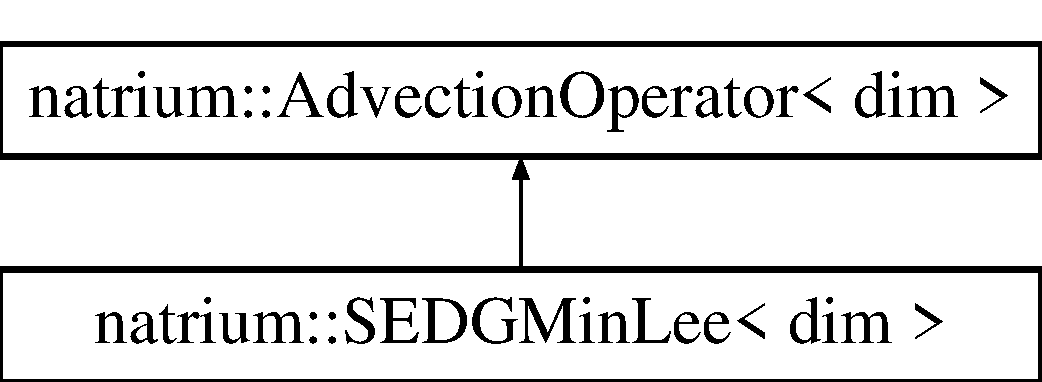
\includegraphics[height=2.000000cm]{classnatrium_1_1AdvectionOperator}
\end{center}
\end{figure}
\subsection*{Public Member Functions}
\begin{DoxyCompactItemize}
\item 
\hypertarget{classnatrium_1_1AdvectionOperator_a48d3a57e3433d9f6c3768ad2f392df56}{\hyperlink{classnatrium_1_1AdvectionOperator_a48d3a57e3433d9f6c3768ad2f392df56}{Advection\-Operator} ()}\label{classnatrium_1_1AdvectionOperator_a48d3a57e3433d9f6c3768ad2f392df56}

\begin{DoxyCompactList}\small\item\em constructor \end{DoxyCompactList}\item 
\hypertarget{classnatrium_1_1AdvectionOperator_a691156dace41e3075fd89953f30ae83f}{virtual \hyperlink{classnatrium_1_1AdvectionOperator_a691156dace41e3075fd89953f30ae83f}{$\sim$\-Advection\-Operator} ()}\label{classnatrium_1_1AdvectionOperator_a691156dace41e3075fd89953f30ae83f}

\begin{DoxyCompactList}\small\item\em destructor \end{DoxyCompactList}\item 
\hypertarget{classnatrium_1_1AdvectionOperator_a89c25c3dae9a1e5973cd89fab8c2c052}{virtual void \hyperlink{classnatrium_1_1AdvectionOperator_a89c25c3dae9a1e5973cd89fab8c2c052}{reassemble} ()=0}\label{classnatrium_1_1AdvectionOperator_a89c25c3dae9a1e5973cd89fab8c2c052}

\begin{DoxyCompactList}\small\item\em function to (re-\/)assemble linear system \end{DoxyCompactList}\item 
\hypertarget{classnatrium_1_1AdvectionOperator_aacdf6096f40166c5ec64686655c906a0}{virtual void \hyperlink{classnatrium_1_1AdvectionOperator_aacdf6096f40166c5ec64686655c906a0}{stream} ()=0}\label{classnatrium_1_1AdvectionOperator_aacdf6096f40166c5ec64686655c906a0}

\begin{DoxyCompactList}\small\item\em make streaming step \end{DoxyCompactList}\item 
\hypertarget{classnatrium_1_1AdvectionOperator_a2cbaee43740d976492e6c9d6d2b84ad0}{virtual const \\*
distributed\-\_\-sparse\-\_\-block\-\_\-matrix \& {\bfseries get\-System\-Matrix} () const =0}\label{classnatrium_1_1AdvectionOperator_a2cbaee43740d976492e6c9d6d2b84ad0}

\item 
\hypertarget{classnatrium_1_1AdvectionOperator_aa1eb5cd5a2c1b6b3b8f6395bac67ef55}{virtual const \\*
distributed\-\_\-block\-\_\-vector \& {\bfseries get\-System\-Vector} () const =0}\label{classnatrium_1_1AdvectionOperator_aa1eb5cd5a2c1b6b3b8f6395bac67ef55}

\item 
\hypertarget{classnatrium_1_1AdvectionOperator_a68f51edd8cc34b61f32ded0a8db82f7b}{virtual const shared\-\_\-ptr\\*
$<$ dealii\-::\-Do\-F\-Handler$<$ dim $>$ $>$ \& {\bfseries get\-Do\-F\-Handler} () const =0}\label{classnatrium_1_1AdvectionOperator_a68f51edd8cc34b61f32ded0a8db82f7b}

\item 
\hypertarget{classnatrium_1_1AdvectionOperator_adc118010e30df45b5906d35743e5ec2e}{virtual void {\bfseries map\-Do\-Fs\-To\-Support\-Points} (vector$<$ dealii\-::\-Point$<$ dim $>$ $>$ \&support\-Points) const =0}\label{classnatrium_1_1AdvectionOperator_adc118010e30df45b5906d35743e5ec2e}

\item 
\hypertarget{classnatrium_1_1AdvectionOperator_a419e94f5534d7871cee47c027a2501c4}{virtual const \\*
dealii\-::\-Mapping\-Q1$<$ dim $>$ \& {\bfseries get\-Mapping} () const =0}\label{classnatrium_1_1AdvectionOperator_a419e94f5534d7871cee47c027a2501c4}

\item 
virtual void \hyperlink{classnatrium_1_1AdvectionOperator_aca14260bae100874b0050a2a96d7a564}{save\-Checkpoint} (const string \&directory) const =0
\begin{DoxyCompactList}\small\item\em save matrices and status to files \end{DoxyCompactList}\item 
\hypertarget{classnatrium_1_1AdvectionOperator_a251e21d1dd023926d4c5f7fd973b90bf}{virtual size\-\_\-t {\bfseries get\-Number\-Of\-Do\-Fs} () const =0}\label{classnatrium_1_1AdvectionOperator_a251e21d1dd023926d4c5f7fd973b90bf}

\end{DoxyCompactItemize}


\subsection{Detailed Description}
\subsubsection*{template$<$size\-\_\-t dim$>$class natrium\-::\-Advection\-Operator$<$ dim $>$}

Abstract class for spatial part of the Advection Operator e\-\_\-i $\ast$ dx\-\_\-i f. 


\begin{DoxyTemplParams}{Template Parameters}
{\em dim} & The dimension of the flow (2 or 3). \\
\hline
\end{DoxyTemplParams}


\subsection{Member Function Documentation}
\hypertarget{classnatrium_1_1AdvectionOperator_aca14260bae100874b0050a2a96d7a564}{\index{natrium\-::\-Advection\-Operator@{natrium\-::\-Advection\-Operator}!save\-Checkpoint@{save\-Checkpoint}}
\index{save\-Checkpoint@{save\-Checkpoint}!natrium::AdvectionOperator@{natrium\-::\-Advection\-Operator}}
\subsubsection[{save\-Checkpoint}]{\setlength{\rightskip}{0pt plus 5cm}template$<$size\-\_\-t dim$>$ virtual void {\bf natrium\-::\-Advection\-Operator}$<$ dim $>$\-::save\-Checkpoint (
\begin{DoxyParamCaption}
\item[{const string \&}]{directory}
\end{DoxyParamCaption}
) const\hspace{0.3cm}{\ttfamily [pure virtual]}}}\label{classnatrium_1_1AdvectionOperator_aca14260bae100874b0050a2a96d7a564}


save matrices and status to files 


\begin{DoxyParams}[1]{Parameters}
\mbox{\tt in}  & {\em directory} & directory to save the matrix files to \\
\hline
\end{DoxyParams}

\begin{DoxyExceptions}{Exceptions}
{\em \hyperlink{classnatrium_1_1AdvectionSolverException}{Advection\-Solver\-Exception}} & \\
\hline
\end{DoxyExceptions}


Implemented in \hyperlink{classnatrium_1_1SEDGMinLee_ab3cf80e18230ee7f08f4ed9883b9dadd}{natrium\-::\-S\-E\-D\-G\-Min\-Lee$<$ dim $>$}.



The documentation for this class was generated from the following file\-:\begin{DoxyCompactItemize}
\item 
/home/kraemer/eclipse\-\_\-workspace/\-N\-A\-Triu\-M/src/natrium/advection/\hyperlink{AdvectionOperator_8h}{Advection\-Operator.\-h}\end{DoxyCompactItemize}

\hypertarget{structnatrium_1_1AdvectionBenchmark_1_1AdvectionResult}{
\section{natrium::AdvectionBenchmark::AdvectionResult Struct Reference}
\label{structnatrium_1_1AdvectionBenchmark_1_1AdvectionResult}\index{natrium::AdvectionBenchmark::AdvectionResult@{natrium::AdvectionBenchmark::AdvectionResult}}
}
\subsection*{Public Attributes}
\begin{DoxyCompactItemize}
\item 
\hypertarget{structnatrium_1_1AdvectionBenchmark_1_1AdvectionResult_ab60c8fdb45a25d1711492f7ff0d5cb24}{
size\_\-t {\bfseries refinementLevel}}
\label{structnatrium_1_1AdvectionBenchmark_1_1AdvectionResult_ab60c8fdb45a25d1711492f7ff0d5cb24}

\item 
\hypertarget{structnatrium_1_1AdvectionBenchmark_1_1AdvectionResult_a0ece16b6c589f53b6ada67e618b914ef}{
size\_\-t {\bfseries fe\_\-order}}
\label{structnatrium_1_1AdvectionBenchmark_1_1AdvectionResult_a0ece16b6c589f53b6ada67e618b914ef}

\item 
\hypertarget{structnatrium_1_1AdvectionBenchmark_1_1AdvectionResult_ae7a2db7be731a116c896d9b31822c504}{
double {\bfseries deltaX}}
\label{structnatrium_1_1AdvectionBenchmark_1_1AdvectionResult_ae7a2db7be731a116c896d9b31822c504}

\item 
\hypertarget{structnatrium_1_1AdvectionBenchmark_1_1AdvectionResult_af7b2e2218885c77be1d35fd67fe0e8d3}{
double {\bfseries deltaT}}
\label{structnatrium_1_1AdvectionBenchmark_1_1AdvectionResult_af7b2e2218885c77be1d35fd67fe0e8d3}

\item 
\hypertarget{structnatrium_1_1AdvectionBenchmark_1_1AdvectionResult_ace3aa8bafc7e3b8f8df4b57fe7f7bbab}{
double {\bfseries norm2}}
\label{structnatrium_1_1AdvectionBenchmark_1_1AdvectionResult_ace3aa8bafc7e3b8f8df4b57fe7f7bbab}

\item 
\hypertarget{structnatrium_1_1AdvectionBenchmark_1_1AdvectionResult_adf5022d425014f41257b51963b76fa5a}{
double {\bfseries normSup}}
\label{structnatrium_1_1AdvectionBenchmark_1_1AdvectionResult_adf5022d425014f41257b51963b76fa5a}

\item 
\hypertarget{structnatrium_1_1AdvectionBenchmark_1_1AdvectionResult_ab3b276d8c638f23e685af5c99aa42370}{
double {\bfseries timesec}}
\label{structnatrium_1_1AdvectionBenchmark_1_1AdvectionResult_ab3b276d8c638f23e685af5c99aa42370}

\end{DoxyCompactItemize}


The documentation for this struct was generated from the following file:\begin{DoxyCompactItemize}
\item 
/mnt/fdrive/akraem3m/workspace/NATriuM/src/library/natrium/benchmarks/AdvectionBenchmark.h\end{DoxyCompactItemize}

\hypertarget{classnatrium_1_1AdvectionSolverException}{
\section{natrium::AdvectionSolverException Class Reference}
\label{classnatrium_1_1AdvectionSolverException}\index{natrium::AdvectionSolverException@{natrium::AdvectionSolverException}}
}


Exception class for \hyperlink{classnatrium_1_1AdvectionOperator}{AdvectionOperator}.  


{\ttfamily \#include $<$AdvectionTools.h$>$}Inheritance diagram for natrium::AdvectionSolverException::\begin{figure}[H]
\begin{center}
\leavevmode
\includegraphics[height=2cm]{classnatrium_1_1AdvectionSolverException}
\end{center}
\end{figure}
\subsection*{Public Member Functions}
\begin{DoxyCompactItemize}
\item 
\hypertarget{classnatrium_1_1AdvectionSolverException_a443084a12dee879bdfbfc900202a0706}{
{\bfseries AdvectionSolverException} (const char $\ast$msg)}
\label{classnatrium_1_1AdvectionSolverException_a443084a12dee879bdfbfc900202a0706}

\item 
\hypertarget{classnatrium_1_1AdvectionSolverException_a9cda3faa279e3528f96c3780a91545bd}{
{\bfseries AdvectionSolverException} (const string \&msg)}
\label{classnatrium_1_1AdvectionSolverException_a9cda3faa279e3528f96c3780a91545bd}

\item 
\hypertarget{classnatrium_1_1AdvectionSolverException_aeb13fafe3f75de7cfd4e282a8a0fb5b0}{
const char $\ast$ {\bfseries what} () const   throw ()}
\label{classnatrium_1_1AdvectionSolverException_aeb13fafe3f75de7cfd4e282a8a0fb5b0}

\end{DoxyCompactItemize}


\subsection{Detailed Description}
Exception class for \hyperlink{classnatrium_1_1AdvectionOperator}{AdvectionOperator}. 

The documentation for this class was generated from the following file:\begin{DoxyCompactItemize}
\item 
/mnt/fdrive/akraem3m/workspace/NATriuM/src/library/natrium/advection/AdvectionTools.h\end{DoxyCompactItemize}

\hypertarget{classnatrium_1_1TaylorGreenVortex2D_1_1AnalyticDensity}{
\section{natrium::TaylorGreenVortex2D::AnalyticDensity Class Reference}
\label{classnatrium_1_1TaylorGreenVortex2D_1_1AnalyticDensity}\index{natrium::TaylorGreenVortex2D::AnalyticDensity@{natrium::TaylorGreenVortex2D::AnalyticDensity}}
}


class to describe the y-\/component of the analytic solution  


{\ttfamily \#include $<$TaylorGreenVortex2D.h$>$}\subsection*{Public Member Functions}
\begin{DoxyCompactItemize}
\item 
\hypertarget{classnatrium_1_1TaylorGreenVortex2D_1_1AnalyticDensity_aabfcf7599f5e512deed9f227fd46b6e7}{
{\bfseries AnalyticDensity} (\hyperlink{classnatrium_1_1TaylorGreenVortex2D}{TaylorGreenVortex2D} $\ast$flow)}
\label{classnatrium_1_1TaylorGreenVortex2D_1_1AnalyticDensity_aabfcf7599f5e512deed9f227fd46b6e7}

\item 
\hypertarget{classnatrium_1_1TaylorGreenVortex2D_1_1AnalyticDensity_a3bfa3988593be2a124fd393f59e17795}{
virtual double {\bfseries value} (const dealii::Point$<$ 2 $>$ \&x, const unsigned int component=0) const }
\label{classnatrium_1_1TaylorGreenVortex2D_1_1AnalyticDensity_a3bfa3988593be2a124fd393f59e17795}

\end{DoxyCompactItemize}


\subsection{Detailed Description}
class to describe the y-\/component of the analytic solution 

The documentation for this class was generated from the following files:\begin{DoxyCompactItemize}
\item 
/mnt/fdrive/akraem3m/workspace/NATriuM/src/library/natrium/benchmarks/\hyperlink{TaylorGreenVortex2D_8h}{TaylorGreenVortex2D.h}\item 
/mnt/fdrive/akraem3m/workspace/NATriuM/src/library/natrium/benchmarks/\hyperlink{TaylorGreenVortex2D_8cpp}{TaylorGreenVortex2D.cpp}\end{DoxyCompactItemize}

\hypertarget{classnatrium_1_1CouetteFlow2D_1_1AnalyticVelocity}{
\section{natrium::CouetteFlow2D::AnalyticVelocity Class Reference}
\label{classnatrium_1_1CouetteFlow2D_1_1AnalyticVelocity}\index{natrium::CouetteFlow2D::AnalyticVelocity@{natrium::CouetteFlow2D::AnalyticVelocity}}
}


class to describe the x-\/component of the analytic solution  


{\ttfamily \#include $<$CouetteFlow2D.h$>$}\subsection*{Public Member Functions}
\begin{DoxyCompactItemize}
\item 
\hypertarget{classnatrium_1_1CouetteFlow2D_1_1AnalyticVelocity_afea6c39b327d7e14b6ebd5b7e8bcd6b8}{
{\bfseries AnalyticVelocity} (\hyperlink{classnatrium_1_1CouetteFlow2D}{CouetteFlow2D} $\ast$couette)}
\label{classnatrium_1_1CouetteFlow2D_1_1AnalyticVelocity_afea6c39b327d7e14b6ebd5b7e8bcd6b8}

\item 
\hypertarget{classnatrium_1_1CouetteFlow2D_1_1AnalyticVelocity_a221bc963c37f2ed82f2a00231e957bfa}{
virtual double {\bfseries value} (const dealii::Point$<$ 2 $>$ \&x, const unsigned int component=0) const }
\label{classnatrium_1_1CouetteFlow2D_1_1AnalyticVelocity_a221bc963c37f2ed82f2a00231e957bfa}

\end{DoxyCompactItemize}


\subsection{Detailed Description}
class to describe the x-\/component of the analytic solution \begin{DoxyNote}{Note}
other are default (v0=w0=0, rho0=1) 
\end{DoxyNote}


The documentation for this class was generated from the following files:\begin{DoxyCompactItemize}
\item 
/mnt/fdrive/akraem3m/workspace/NATriuM/src/library/natrium/benchmarks/\hyperlink{CouetteFlow2D_8h}{CouetteFlow2D.h}\item 
/mnt/fdrive/akraem3m/workspace/NATriuM/src/library/natrium/benchmarks/\hyperlink{CouetteFlow2D_8cpp}{CouetteFlow2D.cpp}\end{DoxyCompactItemize}

\hypertarget{classnatrium_1_1TaylorGreenVortex2D_1_1AnalyticVelocity}{
\section{natrium::TaylorGreenVortex2D::AnalyticVelocity Class Reference}
\label{classnatrium_1_1TaylorGreenVortex2D_1_1AnalyticVelocity}\index{natrium::TaylorGreenVortex2D::AnalyticVelocity@{natrium::TaylorGreenVortex2D::AnalyticVelocity}}
}


class to describe the x-\/component of the analytic solution  


{\ttfamily \#include $<$TaylorGreenVortex2D.h$>$}\subsection*{Public Member Functions}
\begin{DoxyCompactItemize}
\item 
\hypertarget{classnatrium_1_1TaylorGreenVortex2D_1_1AnalyticVelocity_a792726979799a861520617348b4d2c0a}{
{\bfseries AnalyticVelocity} (\hyperlink{classnatrium_1_1TaylorGreenVortex2D}{TaylorGreenVortex2D} $\ast$flow)}
\label{classnatrium_1_1TaylorGreenVortex2D_1_1AnalyticVelocity_a792726979799a861520617348b4d2c0a}

\item 
\hypertarget{classnatrium_1_1TaylorGreenVortex2D_1_1AnalyticVelocity_a9ba30b47d38876999ae49f092b651f86}{
virtual double {\bfseries value} (const dealii::Point$<$ 2 $>$ \&x, const unsigned int component=0) const }
\label{classnatrium_1_1TaylorGreenVortex2D_1_1AnalyticVelocity_a9ba30b47d38876999ae49f092b651f86}

\end{DoxyCompactItemize}


\subsection{Detailed Description}
class to describe the x-\/component of the analytic solution 

The documentation for this class was generated from the following files:\begin{DoxyCompactItemize}
\item 
/mnt/fdrive/akraem3m/workspace/NATriuM/src/library/natrium/benchmarks/\hyperlink{TaylorGreenVortex2D_8h}{TaylorGreenVortex2D.h}\item 
/mnt/fdrive/akraem3m/workspace/NATriuM/src/library/natrium/benchmarks/\hyperlink{TaylorGreenVortex2D_8cpp}{TaylorGreenVortex2D.cpp}\end{DoxyCompactItemize}

\hypertarget{classnatrium_1_1CouetteFlow3D_1_1AnalyticVelocity}{
\section{natrium::CouetteFlow3D::AnalyticVelocity Class Reference}
\label{classnatrium_1_1CouetteFlow3D_1_1AnalyticVelocity}\index{natrium::CouetteFlow3D::AnalyticVelocity@{natrium::CouetteFlow3D::AnalyticVelocity}}
}
\subsection*{Public Member Functions}
\begin{DoxyCompactItemize}
\item 
\hypertarget{classnatrium_1_1CouetteFlow3D_1_1AnalyticVelocity_a52437301be614bb9129fabe6ad91dc12}{
{\bfseries AnalyticVelocity} (\hyperlink{classnatrium_1_1CouetteFlow3D}{CouetteFlow3D} $\ast$couette)}
\label{classnatrium_1_1CouetteFlow3D_1_1AnalyticVelocity_a52437301be614bb9129fabe6ad91dc12}

\item 
\hypertarget{classnatrium_1_1CouetteFlow3D_1_1AnalyticVelocity_a3089b09f900ac2faa7315e85d5b7a809}{
virtual double {\bfseries value} (const dealii::Point$<$ 3 $>$ \&x, const unsigned int component=0) const }
\label{classnatrium_1_1CouetteFlow3D_1_1AnalyticVelocity_a3089b09f900ac2faa7315e85d5b7a809}

\end{DoxyCompactItemize}


The documentation for this class was generated from the following files:\begin{DoxyCompactItemize}
\item 
/mnt/fdrive/akraem3m/workspace/NATriuM/src/library/natrium/benchmarks/\hyperlink{CouetteFlow3D_8h}{CouetteFlow3D.h}\item 
/mnt/fdrive/akraem3m/workspace/NATriuM/src/library/natrium/benchmarks/\hyperlink{CouetteFlow3D_8cpp}{CouetteFlow3D.cpp}\end{DoxyCompactItemize}

\hypertarget{classnatrium_1_1CouetteFlowGrad2D_1_1AnalyticVelocity}{
\section{natrium::CouetteFlowGrad2D::AnalyticVelocity Class Reference}
\label{classnatrium_1_1CouetteFlowGrad2D_1_1AnalyticVelocity}\index{natrium::CouetteFlowGrad2D::AnalyticVelocity@{natrium::CouetteFlowGrad2D::AnalyticVelocity}}
}


class to describe the x-\/component of the analytic solution  


{\ttfamily \#include $<$CouetteFlowGrad2D.h$>$}\subsection*{Public Member Functions}
\begin{DoxyCompactItemize}
\item 
\hypertarget{classnatrium_1_1CouetteFlowGrad2D_1_1AnalyticVelocity_a0000c1ae561e0cb83908149458239bc9}{
{\bfseries AnalyticVelocity} (\hyperlink{classnatrium_1_1CouetteFlowGrad2D}{CouetteFlowGrad2D} $\ast$couette)}
\label{classnatrium_1_1CouetteFlowGrad2D_1_1AnalyticVelocity_a0000c1ae561e0cb83908149458239bc9}

\item 
\hypertarget{classnatrium_1_1CouetteFlowGrad2D_1_1AnalyticVelocity_ae275beccc815763b2b998f474a7331da}{
virtual double {\bfseries value} (const dealii::Point$<$ 2 $>$ \&x, const unsigned int component=0) const }
\label{classnatrium_1_1CouetteFlowGrad2D_1_1AnalyticVelocity_ae275beccc815763b2b998f474a7331da}

\end{DoxyCompactItemize}


\subsection{Detailed Description}
class to describe the x-\/component of the analytic solution \begin{DoxyNote}{Note}
other are default (v0=w0=0, rho0=1) 
\end{DoxyNote}


The documentation for this class was generated from the following files:\begin{DoxyCompactItemize}
\item 
/mnt/fdrive/akraem3m/workspace/NATriuM/src/library/natrium/benchmarks/\hyperlink{CouetteFlowGrad2D_8h}{CouetteFlowGrad2D.h}\item 
/mnt/fdrive/akraem3m/workspace/NATriuM/src/library/natrium/benchmarks/\hyperlink{CouetteFlowGrad2D_8cpp}{CouetteFlowGrad2D.cpp}\end{DoxyCompactItemize}

\hypertarget{classnatrium_1_1PoiseuilleFlow2D_1_1AnalyticVelocity}{
\section{natrium::PoiseuilleFlow2D::AnalyticVelocity Class Reference}
\label{classnatrium_1_1PoiseuilleFlow2D_1_1AnalyticVelocity}\index{natrium::PoiseuilleFlow2D::AnalyticVelocity@{natrium::PoiseuilleFlow2D::AnalyticVelocity}}
}


class to describe the x-\/component of the analytic solution  


{\ttfamily \#include $<$PoiseuilleFlow2D.h$>$}\subsection*{Public Member Functions}
\begin{DoxyCompactItemize}
\item 
\hypertarget{classnatrium_1_1PoiseuilleFlow2D_1_1AnalyticVelocity_a2586adcf8e868b937a1870372ca33d8a}{
{\bfseries AnalyticVelocity} (\hyperlink{classnatrium_1_1PoiseuilleFlow2D}{PoiseuilleFlow2D} $\ast$flow)}
\label{classnatrium_1_1PoiseuilleFlow2D_1_1AnalyticVelocity_a2586adcf8e868b937a1870372ca33d8a}

\item 
\hypertarget{classnatrium_1_1PoiseuilleFlow2D_1_1AnalyticVelocity_a251a3b4a0693bebcf92d7df82b43b436}{
virtual double {\bfseries value} (const dealii::Point$<$ 2 $>$ \&x, const unsigned int component=0) const }
\label{classnatrium_1_1PoiseuilleFlow2D_1_1AnalyticVelocity_a251a3b4a0693bebcf92d7df82b43b436}

\end{DoxyCompactItemize}


\subsection{Detailed Description}
class to describe the x-\/component of the analytic solution \begin{DoxyNote}{Note}
other are default (v0=w0=0, rho0=1) 
\end{DoxyNote}


The documentation for this class was generated from the following files:\begin{DoxyCompactItemize}
\item 
/mnt/fdrive/akraem3m/workspace/NATriuM/src/library/natrium/benchmarks/\hyperlink{PoiseuilleFlow2D_8h}{PoiseuilleFlow2D.h}\item 
/mnt/fdrive/akraem3m/workspace/NATriuM/src/library/natrium/benchmarks/\hyperlink{PoiseuilleFlow2D_8cpp}{PoiseuilleFlow2D.cpp}\end{DoxyCompactItemize}

\hypertarget{classnatrium_1_1PoiseuilleFlow3D_1_1AnalyticVelocity}{
\section{natrium::PoiseuilleFlow3D::AnalyticVelocity Class Reference}
\label{classnatrium_1_1PoiseuilleFlow3D_1_1AnalyticVelocity}\index{natrium::PoiseuilleFlow3D::AnalyticVelocity@{natrium::PoiseuilleFlow3D::AnalyticVelocity}}
}


class to describe the x-\/component of the analytic solution  


{\ttfamily \#include $<$PoiseuilleFlow3D.h$>$}\subsection*{Public Member Functions}
\begin{DoxyCompactItemize}
\item 
\hypertarget{classnatrium_1_1PoiseuilleFlow3D_1_1AnalyticVelocity_ab56ec080a642f5cc3b5b5857bcd915b4}{
{\bfseries AnalyticVelocity} (\hyperlink{classnatrium_1_1PoiseuilleFlow3D}{PoiseuilleFlow3D} $\ast$flow)}
\label{classnatrium_1_1PoiseuilleFlow3D_1_1AnalyticVelocity_ab56ec080a642f5cc3b5b5857bcd915b4}

\item 
\hypertarget{classnatrium_1_1PoiseuilleFlow3D_1_1AnalyticVelocity_ad30167ebbaf4d7f1cec7bf548f3e0dc5}{
virtual double {\bfseries value} (const dealii::Point$<$ 3 $>$ \&x, const unsigned int component=0) const }
\label{classnatrium_1_1PoiseuilleFlow3D_1_1AnalyticVelocity_ad30167ebbaf4d7f1cec7bf548f3e0dc5}

\end{DoxyCompactItemize}


\subsection{Detailed Description}
class to describe the x-\/component of the analytic solution \begin{DoxyNote}{Note}
other are default (v0=w0=0, rho0=1) 
\end{DoxyNote}


The documentation for this class was generated from the following files:\begin{DoxyCompactItemize}
\item 
/mnt/fdrive/akraem3m/workspace/NATriuM/src/library/natrium/benchmarks/\hyperlink{PoiseuilleFlow3D_8h}{PoiseuilleFlow3D.h}\item 
/mnt/fdrive/akraem3m/workspace/NATriuM/src/library/natrium/benchmarks/\hyperlink{PoiseuilleFlow3D_8cpp}{PoiseuilleFlow3D.cpp}\end{DoxyCompactItemize}

\hypertarget{classnatrium_1_1BackwardFacingStep2D}{
\section{natrium::BackwardFacingStep2D Class Reference}
\label{classnatrium_1_1BackwardFacingStep2D}\index{natrium::BackwardFacingStep2D@{natrium::BackwardFacingStep2D}}
}
Inheritance diagram for natrium::BackwardFacingStep2D::\begin{figure}[H]
\begin{center}
\leavevmode
\includegraphics[height=2cm]{classnatrium_1_1BackwardFacingStep2D}
\end{center}
\end{figure}
\subsection*{Classes}
\begin{DoxyCompactItemize}
\item 
class \hyperlink{classnatrium_1_1BackwardFacingStep2D_1_1InflowVelocity}{InflowVelocity}
\item 
class \hyperlink{classnatrium_1_1BackwardFacingStep2D_1_1InitialVelocity}{InitialVelocity}
\begin{DoxyCompactList}\small\item\em class to describe the x-\/component of the analytic solution \item\end{DoxyCompactList}\end{DoxyCompactItemize}
\subsection*{Public Member Functions}
\begin{DoxyCompactItemize}
\item 
\hypertarget{classnatrium_1_1BackwardFacingStep2D_acee242cbe42db517032d784ea9667755}{
\hyperlink{classnatrium_1_1BackwardFacingStep2D_acee242cbe42db517032d784ea9667755}{BackwardFacingStep2D} (double viscosity, double inflow\_\-velocity, size\_\-t refinement\_\-level, double L\_\-domain=18.5, double L\_\-step=2.5, double h\_\-domain=1.0, double h\_\-step=0.5)}
\label{classnatrium_1_1BackwardFacingStep2D_acee242cbe42db517032d784ea9667755}

\begin{DoxyCompactList}\small\item\em constructor \item\end{DoxyCompactList}\item 
\hypertarget{classnatrium_1_1BackwardFacingStep2D_a5eba90130e3ba07642ac092617f81f9d}{
virtual \hyperlink{classnatrium_1_1BackwardFacingStep2D_a5eba90130e3ba07642ac092617f81f9d}{$\sim$BackwardFacingStep2D} ()}
\label{classnatrium_1_1BackwardFacingStep2D_a5eba90130e3ba07642ac092617f81f9d}

\begin{DoxyCompactList}\small\item\em destructor \item\end{DoxyCompactList}\item 
\hypertarget{classnatrium_1_1BackwardFacingStep2D_a6f8e1c7c911c7f15c503530352075218}{
virtual double {\bfseries getCharacteristicVelocity} () const }
\label{classnatrium_1_1BackwardFacingStep2D_a6f8e1c7c911c7f15c503530352075218}

\item 
\hypertarget{classnatrium_1_1BackwardFacingStep2D_a9f1629d0fd14226b3b8360752e62dba2}{
virtual void {\bfseries refine} (Mesh$<$ 2 $>$ \&mesh)}
\label{classnatrium_1_1BackwardFacingStep2D_a9f1629d0fd14226b3b8360752e62dba2}

\item 
\hypertarget{classnatrium_1_1BackwardFacingStep2D_abc272e3f4e2bc5a5fd5aa56c67fe354a}{
virtual void {\bfseries transform} (Mesh$<$ 2 $>$ \&mesh)}
\label{classnatrium_1_1BackwardFacingStep2D_abc272e3f4e2bc5a5fd5aa56c67fe354a}

\item 
\hypertarget{classnatrium_1_1BackwardFacingStep2D_a348a6b0c001ac4bf30b0dfff5f682094}{
virtual bool {\bfseries isCartesian} ()}
\label{classnatrium_1_1BackwardFacingStep2D_a348a6b0c001ac4bf30b0dfff5f682094}

\end{DoxyCompactItemize}


The documentation for this class was generated from the following files:\begin{DoxyCompactItemize}
\item 
/mnt/fdrive/akraem3m/workspace/NATriuM/src/library/natrium/benchmarks/BackwardFacingStep2D.h\item 
/mnt/fdrive/akraem3m/workspace/NATriuM/src/library/natrium/benchmarks/BackwardFacingStep2D.cpp\end{DoxyCompactItemize}

\hypertarget{classnatrium_1_1Benchmark}{
\section{natrium::Benchmark$<$ dim $>$ Class Template Reference}
\label{classnatrium_1_1Benchmark}\index{natrium::Benchmark@{natrium::Benchmark}}
}
Inheritance diagram for natrium::Benchmark$<$ dim $>$::\begin{figure}[H]
\begin{center}
\leavevmode
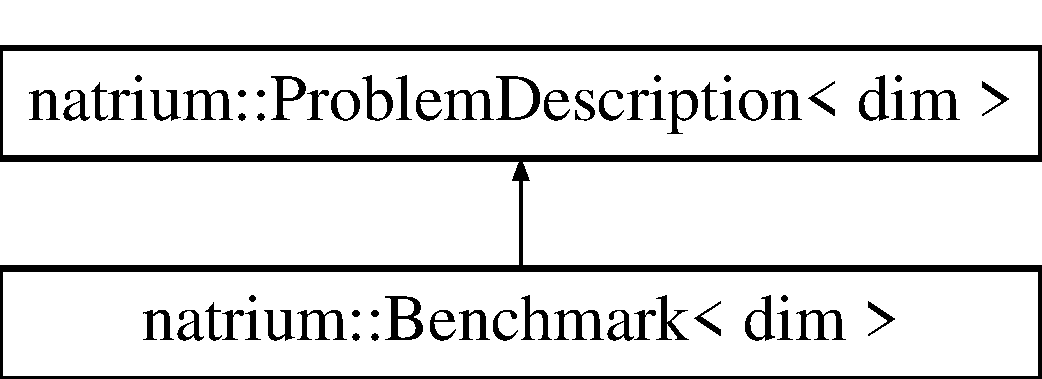
\includegraphics[height=2cm]{classnatrium_1_1Benchmark}
\end{center}
\end{figure}
\subsection*{Public Member Functions}
\begin{DoxyCompactItemize}
\item 
\hypertarget{classnatrium_1_1Benchmark_ae6a264a86ce3a7ca25cb2685e71d6075}{
\hyperlink{classnatrium_1_1Benchmark_ae6a264a86ce3a7ca25cb2685e71d6075}{Benchmark} (boost::shared\_\-ptr$<$ Mesh$<$ dim $>$ $>$ triangulation, double viscosity, double characteristicLength)}
\label{classnatrium_1_1Benchmark_ae6a264a86ce3a7ca25cb2685e71d6075}

\begin{DoxyCompactList}\small\item\em Constructor. \item\end{DoxyCompactList}\item 
\hypertarget{classnatrium_1_1Benchmark_a9560e49a097a369ec972b72fb2873a2e}{
virtual \hyperlink{classnatrium_1_1Benchmark_a9560e49a097a369ec972b72fb2873a2e}{$\sim$Benchmark} ()}
\label{classnatrium_1_1Benchmark_a9560e49a097a369ec972b72fb2873a2e}

\begin{DoxyCompactList}\small\item\em Destructor. \item\end{DoxyCompactList}\item 
\hypertarget{classnatrium_1_1Benchmark_ac3dcec8fee0573c9a9a2a951cc4e5cab}{
const boost::shared\_\-ptr$<$ dealii::Function$<$ dim $>$ $>$ \& {\bfseries getAnalyticRhoFunction} (double time) const }
\label{classnatrium_1_1Benchmark_ac3dcec8fee0573c9a9a2a951cc4e5cab}

\item 
\hypertarget{classnatrium_1_1Benchmark_a13f863e6c53b1872b5ce622a13f3029f}{
const boost::shared\_\-ptr$<$ dealii::Function$<$ dim $>$ $>$ \& {\bfseries getAnalyticUFunction} (double time) const }
\label{classnatrium_1_1Benchmark_a13f863e6c53b1872b5ce622a13f3029f}

\item 
\hypertarget{classnatrium_1_1Benchmark_a0e6506ff88d1612a0277b6ceab77682d}{
virtual const boost::shared\_\-ptr$<$ dealii::Function$<$ dim $>$ $>$ \& {\bfseries getInitialRhoFunction} () const }
\label{classnatrium_1_1Benchmark_a0e6506ff88d1612a0277b6ceab77682d}

\item 
\hypertarget{classnatrium_1_1Benchmark_a41d01e18167c6381bc08363d4f26989b}{
virtual const boost::shared\_\-ptr$<$ dealii::Function$<$ dim $>$ $>$ \& {\bfseries getInitialUFunction} () const }
\label{classnatrium_1_1Benchmark_a41d01e18167c6381bc08363d4f26989b}

\end{DoxyCompactItemize}
\subsection*{Protected Member Functions}
\begin{DoxyCompactItemize}
\item 
\hypertarget{classnatrium_1_1Benchmark_a8fc5c100f71b53f4fce3e91729dc49c1}{
void {\bfseries setAnalyticRho} (boost::shared\_\-ptr$<$ dealii::Function$<$ dim $>$ $>$ ana\_\-rho)}
\label{classnatrium_1_1Benchmark_a8fc5c100f71b53f4fce3e91729dc49c1}

\item 
\hypertarget{classnatrium_1_1Benchmark_aa57db8a63eca5066c0749ab66186d622}{
void {\bfseries setAnalyticU} (boost::shared\_\-ptr$<$ dealii::Function$<$ dim $>$ $>$ ana\_\-u)}
\label{classnatrium_1_1Benchmark_aa57db8a63eca5066c0749ab66186d622}

\end{DoxyCompactItemize}
\subsubsection*{template$<$size\_\-t dim$>$ class natrium::Benchmark$<$ dim $>$}



The documentation for this class was generated from the following file:\begin{DoxyCompactItemize}
\item 
/mnt/fdrive/akraem3m/workspace/NATriuM/src/library/natrium/problemdescription/\hyperlink{Benchmark_8h}{Benchmark.h}\end{DoxyCompactItemize}

\hypertarget{classnatrium_1_1BenchmarkCFDSolver}{
\section{natrium::BenchmarkCFDSolver$<$ dim $>$ Class Template Reference}
\label{classnatrium_1_1BenchmarkCFDSolver}\index{natrium::BenchmarkCFDSolver@{natrium::BenchmarkCFDSolver}}
}


a class that overrides the output function of the CFD solver class with comparisons to a reference solution  


{\ttfamily \#include $<$BenchmarkCFDSolver.h$>$}Inheritance diagram for natrium::BenchmarkCFDSolver$<$ dim $>$::\begin{figure}[H]
\begin{center}
\leavevmode
\includegraphics[height=2cm]{classnatrium_1_1BenchmarkCFDSolver}
\end{center}
\end{figure}
\subsection*{Public Member Functions}
\begin{DoxyCompactItemize}
\item 
\hypertarget{classnatrium_1_1BenchmarkCFDSolver_aa9cdc67e4218230f54d74b0182170705}{
\hyperlink{classnatrium_1_1BenchmarkCFDSolver_aa9cdc67e4218230f54d74b0182170705}{BenchmarkCFDSolver} (boost::shared\_\-ptr$<$ \hyperlink{classnatrium_1_1SolverConfiguration}{SolverConfiguration} $>$ configuration, boost::shared\_\-ptr$<$ \hyperlink{classnatrium_1_1Benchmark}{Benchmark}$<$ dim $>$ $>$ problemDescription)}
\label{classnatrium_1_1BenchmarkCFDSolver_aa9cdc67e4218230f54d74b0182170705}

\begin{DoxyCompactList}\small\item\em constructor \item\end{DoxyCompactList}\item 
\hypertarget{classnatrium_1_1BenchmarkCFDSolver_a9d63cc1e2fe66301533713d4f1ce43a6}{
virtual void \hyperlink{classnatrium_1_1BenchmarkCFDSolver_a9d63cc1e2fe66301533713d4f1ce43a6}{output} (size\_\-t iteration, bool is\_\-final=false)}
\label{classnatrium_1_1BenchmarkCFDSolver_a9d63cc1e2fe66301533713d4f1ce43a6}

\begin{DoxyCompactList}\small\item\em create output data and write to file \item\end{DoxyCompactList}\item 
\hypertarget{classnatrium_1_1BenchmarkCFDSolver_a96be8add7c888ef4e6a1cb41cd2b40f6}{
virtual void \hyperlink{classnatrium_1_1BenchmarkCFDSolver_a96be8add7c888ef4e6a1cb41cd2b40f6}{addAnalyticSolutionToOutput} (dealii::DataOut$<$ dim $>$ \&data\_\-out)}
\label{classnatrium_1_1BenchmarkCFDSolver_a96be8add7c888ef4e6a1cb41cd2b40f6}

\begin{DoxyCompactList}\small\item\em gives the possibility for \hyperlink{classnatrium_1_1Benchmark}{Benchmark} instances to add the analytic solution to output \item\end{DoxyCompactList}\item 
\hypertarget{classnatrium_1_1BenchmarkCFDSolver_aafd3c01db648420ce6d98a8349bdfa09}{
virtual \hyperlink{classnatrium_1_1BenchmarkCFDSolver_aafd3c01db648420ce6d98a8349bdfa09}{$\sim$BenchmarkCFDSolver} ()}
\label{classnatrium_1_1BenchmarkCFDSolver_aafd3c01db648420ce6d98a8349bdfa09}

\begin{DoxyCompactList}\small\item\em destructor \item\end{DoxyCompactList}\item 
\hypertarget{classnatrium_1_1BenchmarkCFDSolver_a486d464112256436c1c3300b28519cbb}{
void \hyperlink{classnatrium_1_1BenchmarkCFDSolver_a486d464112256436c1c3300b28519cbb}{getAllAnalyticDensities} (double time, \hyperlink{namespacenatrium_a903d2b92917f582f2ff05f52160ab811}{distributed\_\-vector} \&analyticDensities, const map$<$ dealii::types::global\_\-dof\_\-index, dealii::Point$<$ dim $>$ $>$ \&supportPoints) const }
\label{classnatrium_1_1BenchmarkCFDSolver_a486d464112256436c1c3300b28519cbb}

\begin{DoxyCompactList}\small\item\em get full analytic solution for the density field at time t \item\end{DoxyCompactList}\item 
\hypertarget{classnatrium_1_1BenchmarkCFDSolver_aebef5814f8c44ab8d0029114b5998cff}{
void \hyperlink{classnatrium_1_1BenchmarkCFDSolver_aebef5814f8c44ab8d0029114b5998cff}{getAllAnalyticVelocities} (double time, vector$<$ \hyperlink{namespacenatrium_a903d2b92917f582f2ff05f52160ab811}{distributed\_\-vector} $>$ \&analyticVelocities, const map$<$ dealii::types::global\_\-dof\_\-index, dealii::Point$<$ dim $>$ $>$ \&supportPoints) const }
\label{classnatrium_1_1BenchmarkCFDSolver_aebef5814f8c44ab8d0029114b5998cff}

\begin{DoxyCompactList}\small\item\em get full analytic solution for the density field at time t \item\end{DoxyCompactList}\item 
void \hyperlink{classnatrium_1_1BenchmarkCFDSolver_a7883dcfd4469ae65ae62cad09ae5d160}{applyInitialVelocities} (vector$<$ \hyperlink{namespacenatrium_a903d2b92917f582f2ff05f52160ab811}{distributed\_\-vector} $>$ \&initialVelocities, const map$<$ dealii::types::global\_\-dof\_\-index, dealii::Point$<$ dim $>$ $>$ \&supportPoints) const 
\begin{DoxyCompactList}\small\item\em set initial velocities \item\end{DoxyCompactList}\item 
\hypertarget{classnatrium_1_1BenchmarkCFDSolver_a767bb620c883abad0091a9e68aee4491}{
const boost::shared\_\-ptr$<$ \hyperlink{classnatrium_1_1Benchmark}{Benchmark}$<$ dim $>$ $>$ \& {\bfseries getBenchmark} () const }
\label{classnatrium_1_1BenchmarkCFDSolver_a767bb620c883abad0091a9e68aee4491}

\item 
\hypertarget{classnatrium_1_1BenchmarkCFDSolver_a659524b149a3650b0f62186e59e385ec}{
const map$<$ dealii::types::global\_\-dof\_\-index, dealii::Point$<$ dim $>$ $>$ \& {\bfseries getSupportPoints} () const }
\label{classnatrium_1_1BenchmarkCFDSolver_a659524b149a3650b0f62186e59e385ec}

\item 
\hypertarget{classnatrium_1_1BenchmarkCFDSolver_abb3b4536d852415a4051c52507514ac2}{
const boost::shared\_\-ptr$<$ \hyperlink{classnatrium_1_1ErrorStats}{ErrorStats}$<$ dim $>$ $>$ \& {\bfseries getErrorStats} () const }
\label{classnatrium_1_1BenchmarkCFDSolver_abb3b4536d852415a4051c52507514ac2}

\end{DoxyCompactItemize}
\subsection*{Friends}
\begin{DoxyCompactItemize}
\item 
\hypertarget{classnatrium_1_1BenchmarkCFDSolver_a168e52694e19bf5c3e3136236b7b6888}{
class {\bfseries ErrorStats}}
\label{classnatrium_1_1BenchmarkCFDSolver_a168e52694e19bf5c3e3136236b7b6888}

\end{DoxyCompactItemize}


\subsection{Detailed Description}
\subsubsection*{template$<$size\_\-t dim$>$ class natrium::BenchmarkCFDSolver$<$ dim $>$}

a class that overrides the output function of the CFD solver class with comparisons to a reference solution 

\subsection{Member Function Documentation}
\hypertarget{classnatrium_1_1BenchmarkCFDSolver_a7883dcfd4469ae65ae62cad09ae5d160}{
\index{natrium::BenchmarkCFDSolver@{natrium::BenchmarkCFDSolver}!applyInitialVelocities@{applyInitialVelocities}}
\index{applyInitialVelocities@{applyInitialVelocities}!natrium::BenchmarkCFDSolver@{natrium::BenchmarkCFDSolver}}
\subsubsection[{applyInitialVelocities}]{\setlength{\rightskip}{0pt plus 5cm}template$<$size\_\-t dim$>$ void {\bf natrium::BenchmarkCFDSolver}$<$ dim $>$::applyInitialVelocities (vector$<$ {\bf distributed\_\-vector} $>$ \& {\em initialVelocities}, \/  const map$<$ dealii::types::global\_\-dof\_\-index, dealii::Point$<$ dim $>$ $>$ \& {\em supportPoints}) const}}
\label{classnatrium_1_1BenchmarkCFDSolver_a7883dcfd4469ae65ae62cad09ae5d160}


set initial velocities 
\begin{DoxyParams}{Parameters}
\item[\mbox{$\rightarrow$} {\em initialVelocities}]vector of velocities; to be filled \item[\mbox{$\leftarrow$} {\em supportPoints}]the coordinates associated with each degree of freedom \end{DoxyParams}


Reimplemented from \hyperlink{classnatrium_1_1CFDSolver_afd82bfa5e1e613ef99b9b870cb73db0e}{natrium::CFDSolver$<$ dim $>$}.

The documentation for this class was generated from the following files:\begin{DoxyCompactItemize}
\item 
/mnt/fdrive/akraem3m/workspace/NATriuM/src/library/natrium/solver/BenchmarkCFDSolver.h\item 
/mnt/fdrive/akraem3m/workspace/NATriuM/src/library/natrium/solver/BenchmarkCFDSolver.cpp\end{DoxyCompactItemize}

\hypertarget{classnatrium_1_1BGK}{
\section{natrium::BGK Class Reference}
\label{classnatrium_1_1BGK}\index{natrium::BGK@{natrium::BGK}}
}


Description of the \hyperlink{classnatrium_1_1BGK}{BGK} model for the transformed particle distributions, as described in Global data which is used by Min and Lee (2011): A spectral-\/element discontinuous Galerkin lattice Boltzmann method for nearly incompressible flows, JCP 230 pp. 245-\/259.  


{\ttfamily \#include $<$BGK.h$>$}Inheritance diagram for natrium::BGK::\begin{figure}[H]
\begin{center}
\leavevmode
\includegraphics[height=1.96262cm]{classnatrium_1_1BGK}
\end{center}
\end{figure}
\subsection*{Public Member Functions}
\begin{DoxyCompactItemize}
\item 
\hyperlink{classnatrium_1_1BGK_adf78ea65d5b96f55dc719b7ab7beb86d}{BGK} (double relaxationParameter, double dt, const boost::shared\_\-ptr$<$ \hyperlink{classnatrium_1_1Stencil}{Stencil} $>$ stencil)
\begin{DoxyCompactList}\small\item\em constructor \item\end{DoxyCompactList}\item 
\hypertarget{classnatrium_1_1BGK_a1029401a72788a6538e4e1941c305ab4}{
virtual \hyperlink{classnatrium_1_1BGK_a1029401a72788a6538e4e1941c305ab4}{$\sim$BGK} ()}
\label{classnatrium_1_1BGK_a1029401a72788a6538e4e1941c305ab4}

\begin{DoxyCompactList}\small\item\em destructor \item\end{DoxyCompactList}\item 
virtual void \hyperlink{classnatrium_1_1BGK_a9fa1c980217a183fc4762954e86ba36d}{collideAll} (\hyperlink{classnatrium_1_1DistributionFunctions}{DistributionFunctions} \&f, distributed\_\-vector \&densities, vector$<$ distributed\_\-vector $>$ \&velocities, const dealii::IndexSet \&locally\_\-owned\_\-dofs, bool inInitializationProcedure=false) const 
\begin{DoxyCompactList}\small\item\em function for collision \item\end{DoxyCompactList}\item 
\hypertarget{classnatrium_1_1BGK_ab82471c249d19fdc62005fb8b7e03190}{
void {\bfseries collideSingleDoF} (size\_\-t doF, const vector$<$ double $>$ \&feq, \hyperlink{classnatrium_1_1DistributionFunctions}{DistributionFunctions} \&f) const }
\label{classnatrium_1_1BGK_ab82471c249d19fdc62005fb8b7e03190}

\item 
\hypertarget{classnatrium_1_1BGK_aebf6d64d5e537c2e352451667d9003d4}{
virtual void \hyperlink{classnatrium_1_1BGK_aebf6d64d5e537c2e352451667d9003d4}{collideSinglePoint} (vector$<$ double $>$ \&distributions) const }
\label{classnatrium_1_1BGK_aebf6d64d5e537c2e352451667d9003d4}

\begin{DoxyCompactList}\small\item\em only for testing purposes; do not use in code, because this function is very inefficient \item\end{DoxyCompactList}\item 
\hypertarget{classnatrium_1_1BGK_acf54bde642d2dc1f83d700fc0a73d575}{
void {\bfseries setRelaxationParameter} (double tau, double dt)}
\label{classnatrium_1_1BGK_acf54bde642d2dc1f83d700fc0a73d575}

\item 
\hypertarget{classnatrium_1_1BGK_a67554c50c9f32d3b51f075988b809b4d}{
double {\bfseries getPrefactor} () const }
\label{classnatrium_1_1BGK_a67554c50c9f32d3b51f075988b809b4d}

\item 
\hypertarget{classnatrium_1_1BGK_a0bbb2526cbfc13c361333a9c32beb0a0}{
void \hyperlink{classnatrium_1_1BGK_a0bbb2526cbfc13c361333a9c32beb0a0}{setTimeStep} (double dt)}
\label{classnatrium_1_1BGK_a0bbb2526cbfc13c361333a9c32beb0a0}

\begin{DoxyCompactList}\small\item\em changes time step and relaxation time at constant velocity and speed of sound \item\end{DoxyCompactList}\item 
\hypertarget{classnatrium_1_1BGK_ab3069be02b1836b1e55c76054c4433a8}{
size\_\-t {\bfseries getQ} () const }
\label{classnatrium_1_1BGK_ab3069be02b1836b1e55c76054c4433a8}

\item 
\hypertarget{classnatrium_1_1BGK_adac002cf79a455f6b053b51210f39acb}{
double {\bfseries getRelaxationParameter} () const }
\label{classnatrium_1_1BGK_adac002cf79a455f6b053b51210f39acb}

\end{DoxyCompactItemize}
\subsection*{Static Public Member Functions}
\begin{DoxyCompactItemize}
\item 
static double \hyperlink{classnatrium_1_1BGK_a430f5020b6101a64d89a0cc2a246260e}{calculateRelaxationParameter} (double viscosity, double timeStepSize, const \hyperlink{classnatrium_1_1Stencil}{Stencil} \&stencil, double=1.0)
\begin{DoxyCompactList}\small\item\em calculate relaxation parameter \item\end{DoxyCompactList}\end{DoxyCompactItemize}


\subsection{Detailed Description}
Description of the \hyperlink{classnatrium_1_1BGK}{BGK} model for the transformed particle distributions, as described in Global data which is used by Min and Lee (2011): A spectral-\/element discontinuous Galerkin lattice Boltzmann method for nearly incompressible flows, JCP 230 pp. 245-\/259. 

\subsection{Constructor \& Destructor Documentation}
\hypertarget{classnatrium_1_1BGK_adf78ea65d5b96f55dc719b7ab7beb86d}{
\index{natrium::BGK@{natrium::BGK}!BGK@{BGK}}
\index{BGK@{BGK}!natrium::BGK@{natrium::BGK}}
\subsubsection[{BGK}]{\setlength{\rightskip}{0pt plus 5cm}natrium::BGK::BGK (double {\em relaxationParameter}, \/  double {\em dt}, \/  const boost::shared\_\-ptr$<$ {\bf Stencil} $>$ {\em stencil})}}
\label{classnatrium_1_1BGK_adf78ea65d5b96f55dc719b7ab7beb86d}


constructor 
\begin{DoxyParams}{Parameters}
\item[\mbox{$\leftarrow$} {\em relaxationParameter}]relaxation parameter tau \end{DoxyParams}


\subsection{Member Function Documentation}
\hypertarget{classnatrium_1_1BGK_a430f5020b6101a64d89a0cc2a246260e}{
\index{natrium::BGK@{natrium::BGK}!calculateRelaxationParameter@{calculateRelaxationParameter}}
\index{calculateRelaxationParameter@{calculateRelaxationParameter}!natrium::BGK@{natrium::BGK}}
\subsubsection[{calculateRelaxationParameter}]{\setlength{\rightskip}{0pt plus 5cm}static double natrium::BGK::calculateRelaxationParameter (double {\em viscosity}, \/  double {\em timeStepSize}, \/  const {\bf Stencil} \& {\em stencil}, \/  double = {\ttfamily 1.0})\hspace{0.3cm}{\ttfamily  \mbox{[}inline, static\mbox{]}}}}
\label{classnatrium_1_1BGK_a430f5020b6101a64d89a0cc2a246260e}


calculate relaxation parameter \begin{DoxyNote}{Note}
preconditioning\_\-parameter is only used for steady state 
\end{DoxyNote}


Reimplemented in \hyperlink{classnatrium_1_1BGKSteadyState_a2cd6628c71475663e204656147de99b8}{natrium::BGKSteadyState}.\hypertarget{classnatrium_1_1BGK_a9fa1c980217a183fc4762954e86ba36d}{
\index{natrium::BGK@{natrium::BGK}!collideAll@{collideAll}}
\index{collideAll@{collideAll}!natrium::BGK@{natrium::BGK}}
\subsubsection[{collideAll}]{\setlength{\rightskip}{0pt plus 5cm}void natrium::BGK::collideAll ({\bf DistributionFunctions} \& {\em f}, \/  distributed\_\-vector \& {\em densities}, \/  vector$<$ distributed\_\-vector $>$ \& {\em velocities}, \/  const dealii::IndexSet \& {\em locally\_\-owned\_\-dofs}, \/  bool {\em inInitializationProcedure} = {\ttfamily false}) const\hspace{0.3cm}{\ttfamily  \mbox{[}virtual\mbox{]}}}}
\label{classnatrium_1_1BGK_a9fa1c980217a183fc4762954e86ba36d}


function for collision f the global vectors of discrete particle distribution functions densities the global vector of densities velocities the global vectors of velocity components \mbox{[} \mbox{[}u\_\-1x, u\_\-2x, ...\mbox{]}, \mbox{[}u\_\-1y, u\_\-2y, ...\mbox{]} \mbox{]} inInitializationProcedure indicates if the collision is performed in the context of an iterative initilizatation procedure. In this case, only the macroscopic densities are recalculated, while the velocities remain unchanged. default: false 

Implements \hyperlink{classnatrium_1_1CollisionModel}{natrium::CollisionModel}.

Reimplemented in \hyperlink{classnatrium_1_1BGKPseudopotential_a5f40f5076273f9ec38f3078c891b453c}{natrium::BGKPseudopotential}, \hyperlink{classnatrium_1_1BGKStandard_a8e0493b063d56275d7ee607e25c4145e}{natrium::BGKStandard}, \hyperlink{classnatrium_1_1BGKStandardTransformed_aaa2e752c6aa2294f1ebeb9d326ba9eb8}{natrium::BGKStandardTransformed}, and \hyperlink{classnatrium_1_1BGKSteadyState_a8554fb624c5a3abe01651747b3d9aeb7}{natrium::BGKSteadyState}.

The documentation for this class was generated from the following files:\begin{DoxyCompactItemize}
\item 
/mnt/fdrive/akraem3m/workspace/NATriuM/src/library/natrium/collision/\hyperlink{BGK_8h}{BGK.h}\item 
/mnt/fdrive/akraem3m/workspace/NATriuM/src/library/natrium/collision/\hyperlink{BGK_8cpp}{BGK.cpp}\end{DoxyCompactItemize}

\hypertarget{classnatrium_1_1BGKIncompressible}{
\section{natrium::BGKIncompressible Class Reference}
\label{classnatrium_1_1BGKIncompressible}\index{natrium::BGKIncompressible@{natrium::BGKIncompressible}}
}
Inheritance diagram for natrium::BGKIncompressible::\begin{figure}[H]
\begin{center}
\leavevmode
\includegraphics[height=3cm]{classnatrium_1_1BGKIncompressible}
\end{center}
\end{figure}
\subsection*{Public Member Functions}
\begin{DoxyCompactItemize}
\item 
\hypertarget{classnatrium_1_1BGKIncompressible_a356e597953a0a7f69ca797a4c15f4039}{
{\bfseries BGKIncompressible} (double relaxationParameter, double dt, const boost::shared\_\-ptr$<$ \hyperlink{classnatrium_1_1Stencil}{Stencil} $>$ stencil)}
\label{classnatrium_1_1BGKIncompressible_a356e597953a0a7f69ca797a4c15f4039}

\item 
virtual double \hyperlink{classnatrium_1_1BGKIncompressible_a26dd8954261b04f8383ca9d37f5ac8c0}{getEquilibriumDistribution} (size\_\-t i, const \hyperlink{namespacenatrium_a67c39077adc6634f8fa3762b8eef24c4}{numeric\_\-vector} \&u, const double rho=1) const 
\begin{DoxyCompactList}\small\item\em function for the calculation of the equilibrium distribution in the incompressible \hyperlink{classnatrium_1_1D2Q9}{D2Q9} model \item\end{DoxyCompactList}\item 
virtual void \hyperlink{classnatrium_1_1BGKIncompressible_a53dc53b5ddb31a6ef67acd25abb405f1}{collideAll} (\hyperlink{classnatrium_1_1DistributionFunctions}{DistributionFunctions} \&f, \hyperlink{namespacenatrium_a903d2b92917f582f2ff05f52160ab811}{distributed\_\-vector} \&densities, vector$<$ \hyperlink{namespacenatrium_a903d2b92917f582f2ff05f52160ab811}{distributed\_\-vector} $>$ \&velocities, const dealii::IndexSet \&locally\_\-owned\_\-dofs, bool inInitializationProcedure=false) const 
\begin{DoxyCompactList}\small\item\em function for collision \item\end{DoxyCompactList}\item 
\hypertarget{classnatrium_1_1BGKIncompressible_aa7f79409678bd0992ca7da81c4632707}{
void \hyperlink{classnatrium_1_1BGKIncompressible_aa7f79409678bd0992ca7da81c4632707}{collideAllD2Q9} (\hyperlink{classnatrium_1_1DistributionFunctions}{DistributionFunctions} \&f, \hyperlink{namespacenatrium_a903d2b92917f582f2ff05f52160ab811}{distributed\_\-vector} \&densities, vector$<$ \hyperlink{namespacenatrium_a903d2b92917f582f2ff05f52160ab811}{distributed\_\-vector} $>$ \&velocities, const dealii::IndexSet \&locally\_\-owned\_\-dofs, bool inInitializationProcedure) const }
\label{classnatrium_1_1BGKIncompressible_aa7f79409678bd0992ca7da81c4632707}

\begin{DoxyCompactList}\small\item\em optimized version of collideAll for \hyperlink{classnatrium_1_1D2Q9}{D2Q9} stencil \item\end{DoxyCompactList}\end{DoxyCompactItemize}


\subsection{Member Function Documentation}
\hypertarget{classnatrium_1_1BGKIncompressible_a53dc53b5ddb31a6ef67acd25abb405f1}{
\index{natrium::BGKIncompressible@{natrium::BGKIncompressible}!collideAll@{collideAll}}
\index{collideAll@{collideAll}!natrium::BGKIncompressible@{natrium::BGKIncompressible}}
\subsubsection[{collideAll}]{\setlength{\rightskip}{0pt plus 5cm}void natrium::BGKIncompressible::collideAll ({\bf DistributionFunctions} \& {\em f}, \/  {\bf distributed\_\-vector} \& {\em densities}, \/  vector$<$ {\bf distributed\_\-vector} $>$ \& {\em velocities}, \/  const dealii::IndexSet \& {\em locally\_\-owned\_\-dofs}, \/  bool {\em inInitializationProcedure} = {\ttfamily false}) const\hspace{0.3cm}{\ttfamily  \mbox{[}virtual\mbox{]}}}}
\label{classnatrium_1_1BGKIncompressible_a53dc53b5ddb31a6ef67acd25abb405f1}


function for collision getEquilibriumDistribution

f the global vectors of discrete particle distribution functions densities the global vector of densities velocities the global vectors of velocity components \mbox{[} \mbox{[}u\_\-1x, u\_\-2x, ...\mbox{]}, \mbox{[}u\_\-1y, u\_\-2y, ...\mbox{]} \mbox{]} inInitializationProcedure indicates if the collision is performed in the context of an iterative initilizatation procedure. In this case, only the macroscopic densities are recalculated, while the velocities remain unchanged. default: false 

Reimplemented from \hyperlink{classnatrium_1_1BGK_a9fa1c980217a183fc4762954e86ba36d}{natrium::BGK}.\hypertarget{classnatrium_1_1BGKIncompressible_a26dd8954261b04f8383ca9d37f5ac8c0}{
\index{natrium::BGKIncompressible@{natrium::BGKIncompressible}!getEquilibriumDistribution@{getEquilibriumDistribution}}
\index{getEquilibriumDistribution@{getEquilibriumDistribution}!natrium::BGKIncompressible@{natrium::BGKIncompressible}}
\subsubsection[{getEquilibriumDistribution}]{\setlength{\rightskip}{0pt plus 5cm}double natrium::BGKIncompressible::getEquilibriumDistribution (size\_\-t {\em i}, \/  const {\bf numeric\_\-vector} \& {\em u}, \/  const double {\em rho} = {\ttfamily 1}) const\hspace{0.3cm}{\ttfamily  \mbox{[}virtual\mbox{]}}}}
\label{classnatrium_1_1BGKIncompressible_a26dd8954261b04f8383ca9d37f5ac8c0}


function for the calculation of the equilibrium distribution in the incompressible \hyperlink{classnatrium_1_1D2Q9}{D2Q9} model 
\begin{DoxyParams}{Parameters}
\item[{\em i}]index of the direction \item[{\em u}]macroscopic velocity \item[{\em rho}]macroscopic density \end{DoxyParams}
\begin{DoxyReturn}{Returns}
value of the equilibrium distribution 
\end{DoxyReturn}
\begin{DoxyNote}{Note}
The calculation can surely be done more efficiently by passing different arguments, e.g. u$\ast$u or u/(c$^\wedge$2) 
\end{DoxyNote}


Implements \hyperlink{classnatrium_1_1CollisionModel_a88b382d63da80e950bc58e8afad769a6}{natrium::CollisionModel}.

The documentation for this class was generated from the following files:\begin{DoxyCompactItemize}
\item 
/mnt/fdrive/akraem3m/workspace/NATriuM/src/library/natrium/collision/\hyperlink{BGKIncompressible_8h}{BGKIncompressible.h}\item 
/mnt/fdrive/akraem3m/workspace/NATriuM/src/library/natrium/collision/\hyperlink{BGKIncompressible_8cpp}{BGKIncompressible.cpp}\end{DoxyCompactItemize}

\hypertarget{classnatrium_1_1BGKMultistep}{
\section{natrium::BGKMultistep Class Reference}
\label{classnatrium_1_1BGKMultistep}\index{natrium::BGKMultistep@{natrium::BGKMultistep}}
}
Inheritance diagram for natrium::BGKMultistep::\begin{figure}[H]
\begin{center}
\leavevmode
\includegraphics[height=3cm]{classnatrium_1_1BGKMultistep}
\end{center}
\end{figure}
\subsection*{Public Types}
\begin{DoxyCompactItemize}
\item 
enum {\bfseries MultistepModelName} \{ {\bfseries ADAMSMOULTON4}, 
{\bfseries BDF2}
 \}
\end{DoxyCompactItemize}
\subsection*{Public Member Functions}
\begin{DoxyCompactItemize}
\item 
\hypertarget{classnatrium_1_1BGKMultistep_ab85df8b619d85553a18fbe8bbb91c2e2}{
{\bfseries BGKMultistep} (double relaxationParameter, double dt, const boost::shared\_\-ptr$<$ \hyperlink{classnatrium_1_1Stencil}{Stencil} $>$ stencil, int model)}
\label{classnatrium_1_1BGKMultistep_ab85df8b619d85553a18fbe8bbb91c2e2}

\item 
virtual double \hyperlink{classnatrium_1_1BGKMultistep_a034cd475974bcce0db64e52245efd91d}{getEquilibriumDistribution} (size\_\-t i, const \hyperlink{namespacenatrium_a67c39077adc6634f8fa3762b8eef24c4}{numeric\_\-vector} \&u, const double rho=1) const 
\begin{DoxyCompactList}\small\item\em virtual function for the calculation of the equilibrium distribution \item\end{DoxyCompactList}\item 
\hypertarget{classnatrium_1_1BGKMultistep_a503d69a669d91979a885d1b02c2edb0a}{
virtual void \hyperlink{classnatrium_1_1BGKMultistep_a503d69a669d91979a885d1b02c2edb0a}{collideAll} (\hyperlink{classnatrium_1_1DistributionFunctions}{DistributionFunctions} \&f, \hyperlink{namespacenatrium_a903d2b92917f582f2ff05f52160ab811}{distributed\_\-vector} \&densities, vector$<$ \hyperlink{namespacenatrium_a903d2b92917f582f2ff05f52160ab811}{distributed\_\-vector} $>$ \&velocities, const dealii::IndexSet \&locally\_\-owned\_\-dofs, bool inInitializationProcedure=false) const }
\label{classnatrium_1_1BGKMultistep_a503d69a669d91979a885d1b02c2edb0a}

\begin{DoxyCompactList}\small\item\em getEquilibriumDistribution \item\end{DoxyCompactList}\item 
void \hyperlink{classnatrium_1_1BGKMultistep_abc9c762511c5dd75a4fc238584a0bc0a}{collideAllD2Q9} (\hyperlink{classnatrium_1_1DistributionFunctions}{DistributionFunctions} \&f, \hyperlink{namespacenatrium_a903d2b92917f582f2ff05f52160ab811}{distributed\_\-vector} \&densities, vector$<$ \hyperlink{namespacenatrium_a903d2b92917f582f2ff05f52160ab811}{distributed\_\-vector} $>$ \&velocities, const dealii::IndexSet \&locally\_\-owned\_\-dofs, bool inInitializationProcedure) const 
\begin{DoxyCompactList}\small\item\em optimized version of collideAll for \hyperlink{classnatrium_1_1D2Q9}{D2Q9} stencil \item\end{DoxyCompactList}\item 
\hypertarget{classnatrium_1_1BGKMultistep_a9b3e71906a2b4399dd048f90c26e2f6a}{
void {\bfseries collideAllD3Q19} (\hyperlink{classnatrium_1_1DistributionFunctions}{DistributionFunctions} \&f, \hyperlink{namespacenatrium_a903d2b92917f582f2ff05f52160ab811}{distributed\_\-vector} \&densities, vector$<$ \hyperlink{namespacenatrium_a903d2b92917f582f2ff05f52160ab811}{distributed\_\-vector} $>$ \&velocities, const dealii::IndexSet \&locally\_\-owned\_\-dofs, bool inInitializationProcedure) const }
\label{classnatrium_1_1BGKMultistep_a9b3e71906a2b4399dd048f90c26e2f6a}

\end{DoxyCompactItemize}
\subsection*{Public Attributes}
\begin{DoxyCompactItemize}
\item 
\hypertarget{classnatrium_1_1BGKMultistep_a23bb03ead6e625d4a2f2830398928a38}{
MultistepModelName {\bfseries m\_\-model}}
\label{classnatrium_1_1BGKMultistep_a23bb03ead6e625d4a2f2830398928a38}

\end{DoxyCompactItemize}


\subsection{Member Function Documentation}
\hypertarget{classnatrium_1_1BGKMultistep_abc9c762511c5dd75a4fc238584a0bc0a}{
\index{natrium::BGKMultistep@{natrium::BGKMultistep}!collideAllD2Q9@{collideAllD2Q9}}
\index{collideAllD2Q9@{collideAllD2Q9}!natrium::BGKMultistep@{natrium::BGKMultistep}}
\subsubsection[{collideAllD2Q9}]{\setlength{\rightskip}{0pt plus 5cm}void natrium::BGKMultistep::collideAllD2Q9 ({\bf DistributionFunctions} \& {\em f}, \/  {\bf distributed\_\-vector} \& {\em densities}, \/  vector$<$ {\bf distributed\_\-vector} $>$ \& {\em velocities}, \/  const dealii::IndexSet \& {\em locally\_\-owned\_\-dofs}, \/  bool {\em inInitializationProcedure}) const}}
\label{classnatrium_1_1BGKMultistep_abc9c762511c5dd75a4fc238584a0bc0a}


optimized version of collideAll for \hyperlink{classnatrium_1_1D2Q9}{D2Q9} stencil 

(scaling $\ast$ scaling); \hypertarget{classnatrium_1_1BGKMultistep_a034cd475974bcce0db64e52245efd91d}{
\index{natrium::BGKMultistep@{natrium::BGKMultistep}!getEquilibriumDistribution@{getEquilibriumDistribution}}
\index{getEquilibriumDistribution@{getEquilibriumDistribution}!natrium::BGKMultistep@{natrium::BGKMultistep}}
\subsubsection[{getEquilibriumDistribution}]{\setlength{\rightskip}{0pt plus 5cm}double natrium::BGKMultistep::getEquilibriumDistribution (size\_\-t {\em i}, \/  const {\bf numeric\_\-vector} \& {\em u}, \/  const double {\em rho} = {\ttfamily 1}) const\hspace{0.3cm}{\ttfamily  \mbox{[}virtual\mbox{]}}}}
\label{classnatrium_1_1BGKMultistep_a034cd475974bcce0db64e52245efd91d}


virtual function for the calculation of the equilibrium distribution 
\begin{DoxyParams}{Parameters}
\item[{\em i}]index of the direction \item[{\em u}]macroscopic velocity \item[{\em rho}]macroscopic density \end{DoxyParams}
\begin{DoxyReturn}{Returns}
value of the equilibrium distribution 
\end{DoxyReturn}
\begin{DoxyNote}{Note}
The calculation can surely be done more efficiently by passing different arguments, e.g. u$\ast$u or u/(c$^\wedge$2) 
\end{DoxyNote}


Implements \hyperlink{classnatrium_1_1CollisionModel_a88b382d63da80e950bc58e8afad769a6}{natrium::CollisionModel}.

The documentation for this class was generated from the following files:\begin{DoxyCompactItemize}
\item 
/mnt/fdrive/akraem3m/workspace/NATriuM/src/library/natrium/collision/BGKMultistep.h\item 
/mnt/fdrive/akraem3m/workspace/NATriuM/src/library/natrium/collision/BGKMultistep.cpp\end{DoxyCompactItemize}

\hypertarget{classnatrium_1_1BGKPseudopotential}{
\section{natrium::BGKPseudopotential$<$ dim $>$ Class Template Reference}
\label{classnatrium_1_1BGKPseudopotential}\index{natrium::BGKPseudopotential@{natrium::BGKPseudopotential}}
}
Inheritance diagram for natrium::BGKPseudopotential$<$ dim $>$::\begin{figure}[H]
\begin{center}
\leavevmode
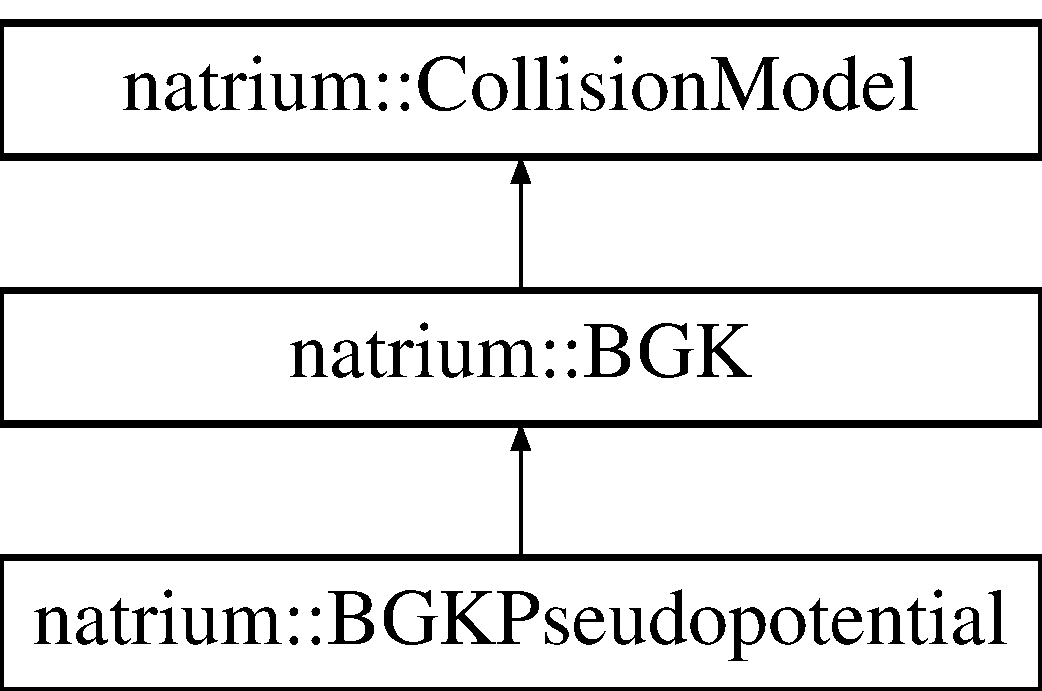
\includegraphics[height=3cm]{classnatrium_1_1BGKPseudopotential}
\end{center}
\end{figure}
\subsection*{Public Member Functions}
\begin{DoxyCompactItemize}
\item 
\hypertarget{classnatrium_1_1BGKPseudopotential_a4400bbf5701254f4cf4363879db54257}{
\hyperlink{classnatrium_1_1BGKPseudopotential_a4400bbf5701254f4cf4363879db54257}{BGKPseudopotential} (double relaxationParameter, double dt, const boost::shared\_\-ptr$<$ \hyperlink{classnatrium_1_1Stencil}{Stencil} $>$ stencil, \hyperlink{structnatrium_1_1PseudopotentialParameters}{PseudopotentialParameters} parameters)}
\label{classnatrium_1_1BGKPseudopotential_a4400bbf5701254f4cf4363879db54257}

\begin{DoxyCompactList}\small\item\em constructor \item\end{DoxyCompactList}\item 
\hypertarget{classnatrium_1_1BGKPseudopotential_a32db75cae893a1d1526f7e18358e5175}{
virtual \hyperlink{classnatrium_1_1BGKPseudopotential_a32db75cae893a1d1526f7e18358e5175}{$\sim$BGKPseudopotential} ()}
\label{classnatrium_1_1BGKPseudopotential_a32db75cae893a1d1526f7e18358e5175}

\begin{DoxyCompactList}\small\item\em destructor \item\end{DoxyCompactList}\item 
virtual double \hyperlink{classnatrium_1_1BGKPseudopotential_a366ccd417ca4ad5fa37ce0572e0d6fe4}{getEquilibriumDistribution} (size\_\-t i, const \hyperlink{namespacenatrium_a67c39077adc6634f8fa3762b8eef24c4}{numeric\_\-vector} \&u, const double rho=1) const 
\begin{DoxyCompactList}\small\item\em virtual function for the calculation of the equilibrium distribution \item\end{DoxyCompactList}\item 
virtual void \hyperlink{classnatrium_1_1BGKPseudopotential_afa18cdab45c73c33b2660f37d0ca82ba}{collideAll} (\hyperlink{classnatrium_1_1DistributionFunctions}{DistributionFunctions} \&f, \hyperlink{namespacenatrium_a903d2b92917f582f2ff05f52160ab811}{distributed\_\-vector} \&densities, vector$<$ \hyperlink{namespacenatrium_a903d2b92917f582f2ff05f52160ab811}{distributed\_\-vector} $>$ \&velocities, const dealii::IndexSet \&locally\_\-owned\_\-dofs, bool inInitializationProcedure=false) const 
\begin{DoxyCompactList}\small\item\em function for collision \item\end{DoxyCompactList}\item 
void \hyperlink{classnatrium_1_1BGKPseudopotential_acf03df141262b39a778e327bf0c25c2a}{collideAllD2Q9} (\hyperlink{classnatrium_1_1DistributionFunctions}{DistributionFunctions} \&f, \hyperlink{namespacenatrium_a903d2b92917f582f2ff05f52160ab811}{distributed\_\-vector} \&densities, vector$<$ \hyperlink{namespacenatrium_a903d2b92917f582f2ff05f52160ab811}{distributed\_\-vector} $>$ \&velocities, bool inInitializationProcedure) const 
\begin{DoxyCompactList}\small\item\em optimized version of collideAll for \hyperlink{classnatrium_1_1D2Q9}{D2Q9} stencil \item\end{DoxyCompactList}\item 
\hypertarget{classnatrium_1_1BGKPseudopotential_a5ac200313ed0ebe9c8df8f179925e2ed}{
void {\bfseries getInteractionForce} (const vector$<$ double $>$ \&distributions, \hyperlink{namespacenatrium_a67c39077adc6634f8fa3762b8eef24c4}{numeric\_\-vector} \&interactionForce, const double rho=1)}
\label{classnatrium_1_1BGKPseudopotential_a5ac200313ed0ebe9c8df8f179925e2ed}

\item 
\hypertarget{classnatrium_1_1BGKPseudopotential_af74dc4543db83980469a322046772e06}{
const boost::shared\_\-ptr$<$ \hyperlink{classnatrium_1_1AdvectionOperator}{AdvectionOperator}$<$ dim $>$ $>$ {\bfseries getAdvectionOperator} () const }
\label{classnatrium_1_1BGKPseudopotential_af74dc4543db83980469a322046772e06}

\item 
\hypertarget{classnatrium_1_1BGKPseudopotential_ab526496c8e4f405355856a6e0ef6a1b1}{
void {\bfseries setAdvectionOperator} (const boost::shared\_\-ptr$<$ \hyperlink{classnatrium_1_1AdvectionOperator}{AdvectionOperator}$<$ dim $>$ $>$ \&advectionOperator)}
\label{classnatrium_1_1BGKPseudopotential_ab526496c8e4f405355856a6e0ef6a1b1}

\end{DoxyCompactItemize}
\subsubsection*{template$<$size\_\-t dim$>$ class natrium::BGKPseudopotential$<$ dim $>$}



\subsection{Member Function Documentation}
\hypertarget{classnatrium_1_1BGKPseudopotential_afa18cdab45c73c33b2660f37d0ca82ba}{
\index{natrium::BGKPseudopotential@{natrium::BGKPseudopotential}!collideAll@{collideAll}}
\index{collideAll@{collideAll}!natrium::BGKPseudopotential@{natrium::BGKPseudopotential}}
\subsubsection[{collideAll}]{\setlength{\rightskip}{0pt plus 5cm}template$<$size\_\-t dim$>$ void {\bf natrium::BGKPseudopotential}$<$ dim $>$::collideAll ({\bf DistributionFunctions} \& {\em f}, \/  {\bf distributed\_\-vector} \& {\em densities}, \/  vector$<$ {\bf distributed\_\-vector} $>$ \& {\em velocities}, \/  const dealii::IndexSet \& {\em locally\_\-owned\_\-dofs}, \/  bool {\em inInitializationProcedure} = {\ttfamily false}) const\hspace{0.3cm}{\ttfamily  \mbox{[}inline, virtual\mbox{]}}}}
\label{classnatrium_1_1BGKPseudopotential_afa18cdab45c73c33b2660f37d0ca82ba}


function for collision f the global vectors of discrete particle distribution functions densities the global vector of densities velocities the global vectors of velocity components \mbox{[} \mbox{[}u\_\-1x, u\_\-2x, ...\mbox{]}, \mbox{[}u\_\-1y, u\_\-2y, ...\mbox{]} \mbox{]} inInitializationProcedure indicates if the collision is performed in the context of an iterative initilizatation procedure. In this case, only the macroscopic densities are recalculated, while the velocities remain unchanged. default: false 

Reimplemented from \hyperlink{classnatrium_1_1BGK_a9fa1c980217a183fc4762954e86ba36d}{natrium::BGK}.\hypertarget{classnatrium_1_1BGKPseudopotential_acf03df141262b39a778e327bf0c25c2a}{
\index{natrium::BGKPseudopotential@{natrium::BGKPseudopotential}!collideAllD2Q9@{collideAllD2Q9}}
\index{collideAllD2Q9@{collideAllD2Q9}!natrium::BGKPseudopotential@{natrium::BGKPseudopotential}}
\subsubsection[{collideAllD2Q9}]{\setlength{\rightskip}{0pt plus 5cm}template$<$size\_\-t dim$>$ void {\bf natrium::BGKPseudopotential}$<$ dim $>$::collideAllD2Q9 ({\bf DistributionFunctions} \& {\em f}, \/  {\bf distributed\_\-vector} \& {\em densities}, \/  vector$<$ {\bf distributed\_\-vector} $>$ \& {\em velocities}, \/  bool {\em inInitializationProcedure}) const\hspace{0.3cm}{\ttfamily  \mbox{[}inline\mbox{]}}}}
\label{classnatrium_1_1BGKPseudopotential_acf03df141262b39a778e327bf0c25c2a}


optimized version of collideAll for \hyperlink{classnatrium_1_1D2Q9}{D2Q9} stencil 

double forceY = (double) 0; \hypertarget{classnatrium_1_1BGKPseudopotential_a366ccd417ca4ad5fa37ce0572e0d6fe4}{
\index{natrium::BGKPseudopotential@{natrium::BGKPseudopotential}!getEquilibriumDistribution@{getEquilibriumDistribution}}
\index{getEquilibriumDistribution@{getEquilibriumDistribution}!natrium::BGKPseudopotential@{natrium::BGKPseudopotential}}
\subsubsection[{getEquilibriumDistribution}]{\setlength{\rightskip}{0pt plus 5cm}template$<$size\_\-t dim$>$ double {\bf natrium::BGKPseudopotential}$<$ dim $>$::getEquilibriumDistribution (size\_\-t {\em i}, \/  const {\bf numeric\_\-vector} \& {\em u}, \/  const double {\em rho} = {\ttfamily 1}) const\hspace{0.3cm}{\ttfamily  \mbox{[}inline, virtual\mbox{]}}}}
\label{classnatrium_1_1BGKPseudopotential_a366ccd417ca4ad5fa37ce0572e0d6fe4}


virtual function for the calculation of the equilibrium distribution 
\begin{DoxyParams}{Parameters}
\item[{\em i}]index of the direction \item[{\em u}]macroscopic velocity \item[{\em rho}]macroscopic density \end{DoxyParams}
\begin{DoxyReturn}{Returns}
value of the equilibrium distribution 
\end{DoxyReturn}
\begin{DoxyNote}{Note}
The calculation can surely be done more efficiently by passing different arguments, e.g. u$\ast$u or u/(c$^\wedge$2) 
\end{DoxyNote}


Implements \hyperlink{classnatrium_1_1CollisionModel_a88b382d63da80e950bc58e8afad769a6}{natrium::CollisionModel}.

The documentation for this class was generated from the following files:\begin{DoxyCompactItemize}
\item 
/mnt/fdrive/akraem3m/workspace/NATriuM/src/library/natrium/collision/BGKPseudopotential.h\item 
/mnt/fdrive/akraem3m/workspace/NATriuM/src/library/natrium/collision/BGKPseudopotential.cpp\end{DoxyCompactItemize}

\hypertarget{classnatrium_1_1BGKStandard}{
\section{natrium::BGKStandard Class Reference}
\label{classnatrium_1_1BGKStandard}\index{natrium::BGKStandard@{natrium::BGKStandard}}
}


Simple \hyperlink{classnatrium_1_1BGK}{BGK} model.  


{\ttfamily \#include $<$BGKStandard.h$>$}Inheritance diagram for natrium::BGKStandard::\begin{figure}[H]
\begin{center}
\leavevmode
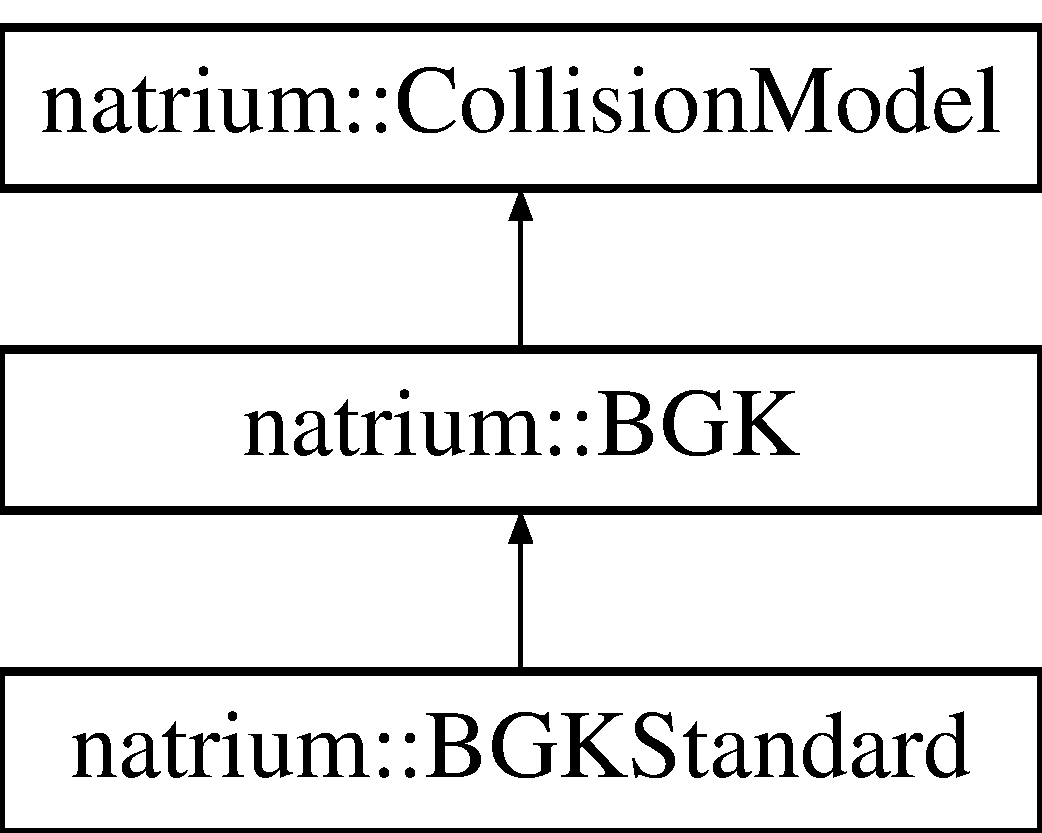
\includegraphics[height=3cm]{classnatrium_1_1BGKStandard}
\end{center}
\end{figure}
\subsection*{Public Member Functions}
\begin{DoxyCompactItemize}
\item 
\hypertarget{classnatrium_1_1BGKStandard_a47cd5ef20c46be121f2e2306f2e6b05b}{
\hyperlink{classnatrium_1_1BGKStandard_a47cd5ef20c46be121f2e2306f2e6b05b}{BGKStandard} (double relaxationParameter, double dt, const shared\_\-ptr$<$ \hyperlink{classnatrium_1_1Stencil}{Stencil} $>$ stencil)}
\label{classnatrium_1_1BGKStandard_a47cd5ef20c46be121f2e2306f2e6b05b}

\begin{DoxyCompactList}\small\item\em constructor \item\end{DoxyCompactList}\item 
virtual \hyperlink{classnatrium_1_1BGKStandard_aa55035be79098a762cf4f0ef308d41e5}{$\sim$BGKStandard} ()
\begin{DoxyCompactList}\small\item\em destructor \item\end{DoxyCompactList}\item 
virtual double \hyperlink{classnatrium_1_1BGKStandard_a3d45ef2fe5536bf14914f99297477754}{getEquilibriumDistribution} (size\_\-t i, const numeric\_\-vector \&u, const double rho=1) const 
\begin{DoxyCompactList}\small\item\em function for the calculation of the equilibrium distribution in the incompressible \hyperlink{classnatrium_1_1D2Q9}{D2Q9} model \item\end{DoxyCompactList}\item 
virtual void \hyperlink{classnatrium_1_1BGKStandard_a8e0493b063d56275d7ee607e25c4145e}{collideAll} (\hyperlink{classnatrium_1_1DistributionFunctions}{DistributionFunctions} \&f, distributed\_\-vector \&densities, vector$<$ distributed\_\-vector $>$ \&velocities, const dealii::IndexSet \&locally\_\-owned\_\-dofs, bool inInitializationProcedure=false) const 
\begin{DoxyCompactList}\small\item\em function for collision \item\end{DoxyCompactList}\end{DoxyCompactItemize}


\subsection{Detailed Description}
Simple \hyperlink{classnatrium_1_1BGK}{BGK} model. 

\subsection{Constructor \& Destructor Documentation}
\hypertarget{classnatrium_1_1BGKStandard_aa55035be79098a762cf4f0ef308d41e5}{
\index{natrium::BGKStandard@{natrium::BGKStandard}!$\sim$BGKStandard@{$\sim$BGKStandard}}
\index{$\sim$BGKStandard@{$\sim$BGKStandard}!natrium::BGKStandard@{natrium::BGKStandard}}
\subsubsection[{$\sim$BGKStandard}]{\setlength{\rightskip}{0pt plus 5cm}natrium::BGKStandard::$\sim$BGKStandard ()\hspace{0.3cm}{\ttfamily  \mbox{[}virtual\mbox{]}}}}
\label{classnatrium_1_1BGKStandard_aa55035be79098a762cf4f0ef308d41e5}


destructor constructor 

\subsection{Member Function Documentation}
\hypertarget{classnatrium_1_1BGKStandard_a8e0493b063d56275d7ee607e25c4145e}{
\index{natrium::BGKStandard@{natrium::BGKStandard}!collideAll@{collideAll}}
\index{collideAll@{collideAll}!natrium::BGKStandard@{natrium::BGKStandard}}
\subsubsection[{collideAll}]{\setlength{\rightskip}{0pt plus 5cm}void natrium::BGKStandard::collideAll ({\bf DistributionFunctions} \& {\em f}, \/  distributed\_\-vector \& {\em densities}, \/  vector$<$ distributed\_\-vector $>$ \& {\em velocities}, \/  const dealii::IndexSet \& {\em locally\_\-owned\_\-dofs}, \/  bool {\em inInitializationProcedure} = {\ttfamily false}) const\hspace{0.3cm}{\ttfamily  \mbox{[}virtual\mbox{]}}}}
\label{classnatrium_1_1BGKStandard_a8e0493b063d56275d7ee607e25c4145e}


function for collision getEquilibriumDistribution

f the global vectors of discrete particle distribution functions densities the global vector of densities velocities the global vectors of velocity components \mbox{[} \mbox{[}u\_\-1x, u\_\-2x, ...\mbox{]}, \mbox{[}u\_\-1y, u\_\-2y, ...\mbox{]} \mbox{]} inInitializationProcedure indicates if the collision is performed in the context of an iterative initilizatation procedure. In this case, only the macroscopic densities are recalculated, while the velocities remain unchanged. default: false 

Reimplemented from \hyperlink{classnatrium_1_1BGK_a9fa1c980217a183fc4762954e86ba36d}{natrium::BGK}.\hypertarget{classnatrium_1_1BGKStandard_a3d45ef2fe5536bf14914f99297477754}{
\index{natrium::BGKStandard@{natrium::BGKStandard}!getEquilibriumDistribution@{getEquilibriumDistribution}}
\index{getEquilibriumDistribution@{getEquilibriumDistribution}!natrium::BGKStandard@{natrium::BGKStandard}}
\subsubsection[{getEquilibriumDistribution}]{\setlength{\rightskip}{0pt plus 5cm}double natrium::BGKStandard::getEquilibriumDistribution (size\_\-t {\em i}, \/  const numeric\_\-vector \& {\em u}, \/  const double {\em rho} = {\ttfamily 1}) const\hspace{0.3cm}{\ttfamily  \mbox{[}virtual\mbox{]}}}}
\label{classnatrium_1_1BGKStandard_a3d45ef2fe5536bf14914f99297477754}


function for the calculation of the equilibrium distribution in the incompressible \hyperlink{classnatrium_1_1D2Q9}{D2Q9} model destructor


\begin{DoxyParams}{Parameters}
\item[{\em i}]index of the direction \item[{\em u}]macroscopic velocity \item[{\em rho}]macroscopic density \end{DoxyParams}
\begin{DoxyReturn}{Returns}
value of the equilibrium distribution 
\end{DoxyReturn}
\begin{DoxyNote}{Note}
The calculation can surely be done more efficiently by passing different arguments, e.g. u$\ast$u or u/(c$^\wedge$2) 
\end{DoxyNote}


Implements \hyperlink{classnatrium_1_1CollisionModel_a88b382d63da80e950bc58e8afad769a6}{natrium::CollisionModel}.

The documentation for this class was generated from the following files:\begin{DoxyCompactItemize}
\item 
/mnt/fdrive/akraem3m/workspace/NATriuM/src/library/natrium/collision/\hyperlink{BGKStandard_8h}{BGKStandard.h}\item 
/mnt/fdrive/akraem3m/workspace/NATriuM/src/library/natrium/collision/\hyperlink{BGKStandard_8cpp}{BGKStandard.cpp}\end{DoxyCompactItemize}

\hypertarget{classnatrium_1_1BGKStandardTransformed}{
\section{natrium::BGKStandardTransformed Class Reference}
\label{classnatrium_1_1BGKStandardTransformed}\index{natrium::BGKStandardTransformed@{natrium::BGKStandardTransformed}}
}


Simple \hyperlink{classnatrium_1_1BGK}{BGK} model with transformed distributions in order to lower round-\/off errors The scheme is described in \char`\"{}How to improve the accuracy of Lattice Boltzmann calculations\char`\"{} by Bastien Chopard (May 2008), available on LBMethod.org.  


{\ttfamily \#include $<$BGKStandardTransformed.h$>$}Inheritance diagram for natrium::BGKStandardTransformed::\begin{figure}[H]
\begin{center}
\leavevmode
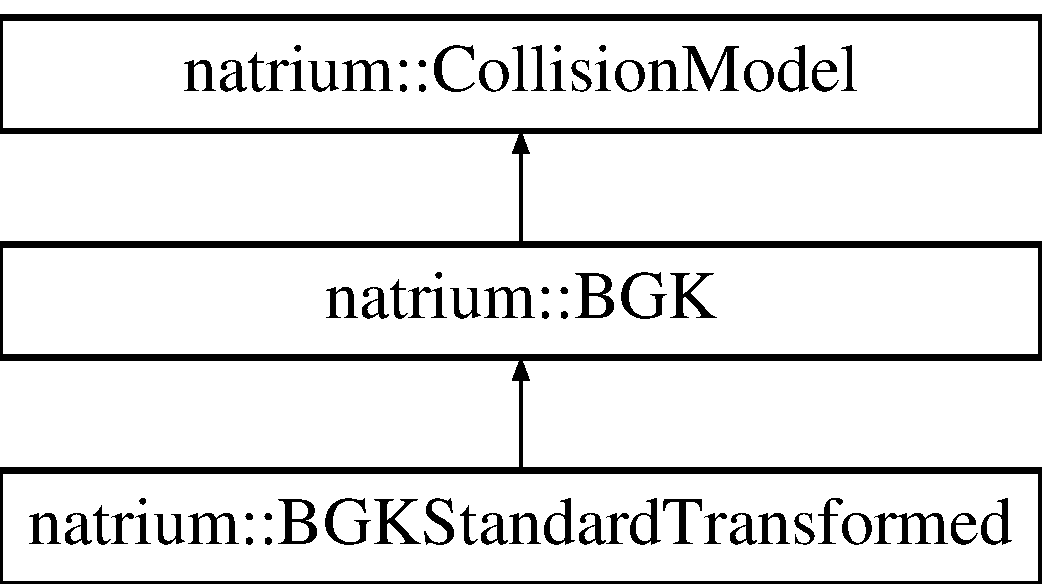
\includegraphics[height=3cm]{classnatrium_1_1BGKStandardTransformed}
\end{center}
\end{figure}
\subsection*{Public Member Functions}
\begin{DoxyCompactItemize}
\item 
\hypertarget{classnatrium_1_1BGKStandardTransformed_ae53d86d6ae640cc598b152538e347737}{
\hyperlink{classnatrium_1_1BGKStandardTransformed_ae53d86d6ae640cc598b152538e347737}{BGKStandardTransformed} (double relaxationParameter, double dt, const boost::shared\_\-ptr$<$ \hyperlink{classnatrium_1_1Stencil}{Stencil} $>$ stencil)}
\label{classnatrium_1_1BGKStandardTransformed_ae53d86d6ae640cc598b152538e347737}

\begin{DoxyCompactList}\small\item\em constructor \item\end{DoxyCompactList}\item 
virtual \hyperlink{classnatrium_1_1BGKStandardTransformed_a07dc7f5ccaf1abaa725a7b62a2b79ac4}{$\sim$BGKStandardTransformed} ()
\begin{DoxyCompactList}\small\item\em destructor \item\end{DoxyCompactList}\item 
virtual double \hyperlink{classnatrium_1_1BGKStandardTransformed_a870465cc026f92c8ffba899af6f95634}{getEquilibriumDistribution} (size\_\-t i, const \hyperlink{namespacenatrium_a67c39077adc6634f8fa3762b8eef24c4}{numeric\_\-vector} \&u, const double rho=1) const 
\begin{DoxyCompactList}\small\item\em function for the calculation of the equilibrium distribution in the incompressible \hyperlink{classnatrium_1_1D2Q9}{D2Q9} model \item\end{DoxyCompactList}\item 
virtual void \hyperlink{classnatrium_1_1BGKStandardTransformed_aaa2e752c6aa2294f1ebeb9d326ba9eb8}{collideAll} (\hyperlink{classnatrium_1_1DistributionFunctions}{DistributionFunctions} \&f, \hyperlink{namespacenatrium_a903d2b92917f582f2ff05f52160ab811}{distributed\_\-vector} \&densities, vector$<$ \hyperlink{namespacenatrium_a903d2b92917f582f2ff05f52160ab811}{distributed\_\-vector} $>$ \&velocities, const dealii::IndexSet \&locally\_\-owned\_\-dofs, bool inInitializationProcedure=false) const 
\begin{DoxyCompactList}\small\item\em function for collision \item\end{DoxyCompactList}\item 
\hypertarget{classnatrium_1_1BGKStandardTransformed_a883401ad796f196bcc47456b31159eae}{
double {\bfseries getRho0} () const }
\label{classnatrium_1_1BGKStandardTransformed_a883401ad796f196bcc47456b31159eae}

\item 
virtual double \hyperlink{classnatrium_1_1BGKStandardTransformed_a58c4dc0c67ff4898c6555b614afc1ace}{calculateDensity} (const vector$<$ double $>$ \&distributions) const 
\begin{DoxyCompactList}\small\item\em calculate macroscopic density \item\end{DoxyCompactList}\end{DoxyCompactItemize}


\subsection{Detailed Description}
Simple \hyperlink{classnatrium_1_1BGK}{BGK} model with transformed distributions in order to lower round-\/off errors The scheme is described in \char`\"{}How to improve the accuracy of Lattice Boltzmann calculations\char`\"{} by Bastien Chopard (May 2008), available on LBMethod.org. 

\subsection{Constructor \& Destructor Documentation}
\hypertarget{classnatrium_1_1BGKStandardTransformed_a07dc7f5ccaf1abaa725a7b62a2b79ac4}{
\index{natrium::BGKStandardTransformed@{natrium::BGKStandardTransformed}!$\sim$BGKStandardTransformed@{$\sim$BGKStandardTransformed}}
\index{$\sim$BGKStandardTransformed@{$\sim$BGKStandardTransformed}!natrium::BGKStandardTransformed@{natrium::BGKStandardTransformed}}
\subsubsection[{$\sim$BGKStandardTransformed}]{\setlength{\rightskip}{0pt plus 5cm}natrium::BGKStandardTransformed::$\sim$BGKStandardTransformed ()\hspace{0.3cm}{\ttfamily  \mbox{[}virtual\mbox{]}}}}
\label{classnatrium_1_1BGKStandardTransformed_a07dc7f5ccaf1abaa725a7b62a2b79ac4}


destructor constructor 

\subsection{Member Function Documentation}
\hypertarget{classnatrium_1_1BGKStandardTransformed_a58c4dc0c67ff4898c6555b614afc1ace}{
\index{natrium::BGKStandardTransformed@{natrium::BGKStandardTransformed}!calculateDensity@{calculateDensity}}
\index{calculateDensity@{calculateDensity}!natrium::BGKStandardTransformed@{natrium::BGKStandardTransformed}}
\subsubsection[{calculateDensity}]{\setlength{\rightskip}{0pt plus 5cm}virtual double natrium::BGKStandardTransformed::calculateDensity (const vector$<$ double $>$ \& {\em distributions}) const\hspace{0.3cm}{\ttfamily  \mbox{[}inline, virtual\mbox{]}}}}
\label{classnatrium_1_1BGKStandardTransformed_a58c4dc0c67ff4898c6555b614afc1ace}


calculate macroscopic density 
\begin{DoxyParams}{Parameters}
\item[\mbox{$\leftarrow$} {\em distributions}]particle distribution functions at a given point \end{DoxyParams}
\begin{DoxyReturn}{Returns}
macroscopic density (sum of all distributions) 
\end{DoxyReturn}


Reimplemented from \hyperlink{classnatrium_1_1CollisionModel_ae1c879c87ac210a227a8e3da2d0ac385}{natrium::CollisionModel}.\hypertarget{classnatrium_1_1BGKStandardTransformed_aaa2e752c6aa2294f1ebeb9d326ba9eb8}{
\index{natrium::BGKStandardTransformed@{natrium::BGKStandardTransformed}!collideAll@{collideAll}}
\index{collideAll@{collideAll}!natrium::BGKStandardTransformed@{natrium::BGKStandardTransformed}}
\subsubsection[{collideAll}]{\setlength{\rightskip}{0pt plus 5cm}void natrium::BGKStandardTransformed::collideAll ({\bf DistributionFunctions} \& {\em f}, \/  {\bf distributed\_\-vector} \& {\em densities}, \/  vector$<$ {\bf distributed\_\-vector} $>$ \& {\em velocities}, \/  const dealii::IndexSet \& {\em locally\_\-owned\_\-dofs}, \/  bool {\em inInitializationProcedure} = {\ttfamily false}) const\hspace{0.3cm}{\ttfamily  \mbox{[}virtual\mbox{]}}}}
\label{classnatrium_1_1BGKStandardTransformed_aaa2e752c6aa2294f1ebeb9d326ba9eb8}


function for collision getEquilibriumDistribution

f the global vectors of discrete particle distribution functions densities the global vector of densities velocities the global vectors of velocity components \mbox{[} \mbox{[}u\_\-1x, u\_\-2x, ...\mbox{]}, \mbox{[}u\_\-1y, u\_\-2y, ...\mbox{]} \mbox{]} inInitializationProcedure indicates if the collision is performed in the context of an iterative initilizatation procedure. In this case, only the macroscopic densities are recalculated, while the velocities remain unchanged. default: false 

Reimplemented from \hyperlink{classnatrium_1_1BGK_a9fa1c980217a183fc4762954e86ba36d}{natrium::BGK}.\hypertarget{classnatrium_1_1BGKStandardTransformed_a870465cc026f92c8ffba899af6f95634}{
\index{natrium::BGKStandardTransformed@{natrium::BGKStandardTransformed}!getEquilibriumDistribution@{getEquilibriumDistribution}}
\index{getEquilibriumDistribution@{getEquilibriumDistribution}!natrium::BGKStandardTransformed@{natrium::BGKStandardTransformed}}
\subsubsection[{getEquilibriumDistribution}]{\setlength{\rightskip}{0pt plus 5cm}double natrium::BGKStandardTransformed::getEquilibriumDistribution (size\_\-t {\em i}, \/  const {\bf numeric\_\-vector} \& {\em u}, \/  const double {\em rho} = {\ttfamily 1}) const\hspace{0.3cm}{\ttfamily  \mbox{[}virtual\mbox{]}}}}
\label{classnatrium_1_1BGKStandardTransformed_a870465cc026f92c8ffba899af6f95634}


function for the calculation of the equilibrium distribution in the incompressible \hyperlink{classnatrium_1_1D2Q9}{D2Q9} model destructor


\begin{DoxyParams}{Parameters}
\item[{\em i}]index of the direction \item[{\em u}]macroscopic velocity \item[{\em rho}]macroscopic density \end{DoxyParams}
\begin{DoxyReturn}{Returns}
value of the equilibrium distribution 
\end{DoxyReturn}
\begin{DoxyNote}{Note}
The calculation can surely be done more efficiently by passing different arguments, e.g. u$\ast$u or u/(c$^\wedge$2) 
\end{DoxyNote}


Implements \hyperlink{classnatrium_1_1CollisionModel_a88b382d63da80e950bc58e8afad769a6}{natrium::CollisionModel}.

The documentation for this class was generated from the following files:\begin{DoxyCompactItemize}
\item 
/mnt/fdrive/akraem3m/workspace/NATriuM/src/library/natrium/collision/\hyperlink{BGKStandardTransformed_8h}{BGKStandardTransformed.h}\item 
/mnt/fdrive/akraem3m/workspace/NATriuM/src/library/natrium/collision/\hyperlink{BGKStandardTransformed_8cpp}{BGKStandardTransformed.cpp}\end{DoxyCompactItemize}

\hypertarget{classnatrium_1_1BGKSteadyState}{
\section{natrium::BGKSteadyState Class Reference}
\label{classnatrium_1_1BGKSteadyState}\index{natrium::BGKSteadyState@{natrium::BGKSteadyState}}
}


\hyperlink{classnatrium_1_1BGK}{BGK} model for preconditioned Navier-\/Stokes equation Paper by Guo et al. (2004): Preconditioned lattice-\/Boltzmann method for steady flows, Physical Review E 70. The equilibrium distribution functions agrees with the one of the standard \hyperlink{classnatrium_1_1BGK}{BGK} model, except it has the factor \[\frac{1}{\gamma}\] with each \[ O(u^2) \] term. The hydrodynamic equations of the Steady State \hyperlink{classnatrium_1_1BGK}{BGK} can be derived by the Chapman-\/Enskog analysis. Except for the temporal derivative, the compressible Navier-\/Stokes equation is found, but with a much better eigenvalue system. This makes the preconditioned \hyperlink{classnatrium_1_1BGK}{BGK} perfect for steady flows, although not physical for unsteady flows.  


{\ttfamily \#include $<$BGKSteadyState.h$>$}Inheritance diagram for natrium::BGKSteadyState::\begin{figure}[H]
\begin{center}
\leavevmode
\includegraphics[height=3cm]{classnatrium_1_1BGKSteadyState}
\end{center}
\end{figure}
\subsection*{Public Member Functions}
\begin{DoxyCompactItemize}
\item 
\hyperlink{classnatrium_1_1BGKSteadyState_aa8521523f8603fdc5a391d6e6388667c}{BGKSteadyState} (double relaxationParameter, double dt, const shared\_\-ptr$<$ \hyperlink{classnatrium_1_1Stencil}{Stencil} $>$ stencil, double preconditioning\_\-parameter)
\begin{DoxyCompactList}\small\item\em Constructor. \item\end{DoxyCompactList}\item 
virtual \hyperlink{classnatrium_1_1BGKSteadyState_ab2c58f1d6b964179a2abeb5f54aa5edc}{$\sim$BGKSteadyState} ()
\begin{DoxyCompactList}\small\item\em destructor \item\end{DoxyCompactList}\item 
virtual double \hyperlink{classnatrium_1_1BGKSteadyState_ad99d9159cc14b5897bea7f145c3b39ca}{getEquilibriumDistribution} (size\_\-t i, const numeric\_\-vector \&u, const double rho=1) const 
\begin{DoxyCompactList}\small\item\em function for the calculation of the equilibrium distribution in the incompressible \hyperlink{classnatrium_1_1D2Q9}{D2Q9} model \item\end{DoxyCompactList}\item 
virtual void \hyperlink{classnatrium_1_1BGKSteadyState_a8554fb624c5a3abe01651747b3d9aeb7}{collideAll} (\hyperlink{classnatrium_1_1DistributionFunctions}{DistributionFunctions} \&f, distributed\_\-vector \&densities, vector$<$ distributed\_\-vector $>$ \&velocities, const dealii::IndexSet \&locally\_\-owned\_\-dofs, bool inInitializationProcedure=false) const 
\begin{DoxyCompactList}\small\item\em function for collision \item\end{DoxyCompactList}\end{DoxyCompactItemize}
\subsection*{Static Public Member Functions}
\begin{DoxyCompactItemize}
\item 
static double \hyperlink{classnatrium_1_1BGKSteadyState_a2cd6628c71475663e204656147de99b8}{calculateRelaxationParameter} (double viscosity, double timeStepSize, const \hyperlink{classnatrium_1_1Stencil}{Stencil} \&stencil, double preconditioning\_\-parameter)
\begin{DoxyCompactList}\small\item\em calculate relaxation parameter \item\end{DoxyCompactList}\end{DoxyCompactItemize}


\subsection{Detailed Description}
\hyperlink{classnatrium_1_1BGK}{BGK} model for preconditioned Navier-\/Stokes equation Paper by Guo et al. (2004): Preconditioned lattice-\/Boltzmann method for steady flows, Physical Review E 70. The equilibrium distribution functions agrees with the one of the standard \hyperlink{classnatrium_1_1BGK}{BGK} model, except it has the factor \[\frac{1}{\gamma}\] with each \[ O(u^2) \] term. The hydrodynamic equations of the Steady State \hyperlink{classnatrium_1_1BGK}{BGK} can be derived by the Chapman-\/Enskog analysis. Except for the temporal derivative, the compressible Navier-\/Stokes equation is found, but with a much better eigenvalue system. This makes the preconditioned \hyperlink{classnatrium_1_1BGK}{BGK} perfect for steady flows, although not physical for unsteady flows. 

\subsection{Constructor \& Destructor Documentation}
\hypertarget{classnatrium_1_1BGKSteadyState_aa8521523f8603fdc5a391d6e6388667c}{
\index{natrium::BGKSteadyState@{natrium::BGKSteadyState}!BGKSteadyState@{BGKSteadyState}}
\index{BGKSteadyState@{BGKSteadyState}!natrium::BGKSteadyState@{natrium::BGKSteadyState}}
\subsubsection[{BGKSteadyState}]{\setlength{\rightskip}{0pt plus 5cm}natrium::BGKSteadyState::BGKSteadyState (double {\em relaxationParameter}, \/  double {\em dt}, \/  const shared\_\-ptr$<$ {\bf Stencil} $>$ {\em stencil}, \/  double {\em preconditioning\_\-parameter})}}
\label{classnatrium_1_1BGKSteadyState_aa8521523f8603fdc5a391d6e6388667c}


Constructor. constructor


\begin{DoxyParams}{Parameters}
\item[{\em preconditioning\_\-parameter}](\[ \gamma \in (0,1] \] is the preconditioning parameter \[ \gamma = 1 \] gives the standard \hyperlink{classnatrium_1_1BGK}{BGK} model, for \[ \gamma \leftarrow 0 \], the effective sound speed is decreased \end{DoxyParams}
\hypertarget{classnatrium_1_1BGKSteadyState_ab2c58f1d6b964179a2abeb5f54aa5edc}{
\index{natrium::BGKSteadyState@{natrium::BGKSteadyState}!$\sim$BGKSteadyState@{$\sim$BGKSteadyState}}
\index{$\sim$BGKSteadyState@{$\sim$BGKSteadyState}!natrium::BGKSteadyState@{natrium::BGKSteadyState}}
\subsubsection[{$\sim$BGKSteadyState}]{\setlength{\rightskip}{0pt plus 5cm}natrium::BGKSteadyState::$\sim$BGKSteadyState ()\hspace{0.3cm}{\ttfamily  \mbox{[}virtual\mbox{]}}}}
\label{classnatrium_1_1BGKSteadyState_ab2c58f1d6b964179a2abeb5f54aa5edc}


destructor constructor 

\subsection{Member Function Documentation}
\hypertarget{classnatrium_1_1BGKSteadyState_a2cd6628c71475663e204656147de99b8}{
\index{natrium::BGKSteadyState@{natrium::BGKSteadyState}!calculateRelaxationParameter@{calculateRelaxationParameter}}
\index{calculateRelaxationParameter@{calculateRelaxationParameter}!natrium::BGKSteadyState@{natrium::BGKSteadyState}}
\subsubsection[{calculateRelaxationParameter}]{\setlength{\rightskip}{0pt plus 5cm}static double natrium::BGKSteadyState::calculateRelaxationParameter (double {\em viscosity}, \/  double {\em timeStepSize}, \/  const {\bf Stencil} \& {\em stencil}, \/  double {\em preconditioning\_\-parameter})\hspace{0.3cm}{\ttfamily  \mbox{[}inline, static\mbox{]}}}}
\label{classnatrium_1_1BGKSteadyState_a2cd6628c71475663e204656147de99b8}


calculate relaxation parameter \begin{DoxyNote}{Note}
the preconditioning parameter gamma is only used for steady state 
\end{DoxyNote}


Reimplemented from \hyperlink{classnatrium_1_1BGK_a430f5020b6101a64d89a0cc2a246260e}{natrium::BGK}.\hypertarget{classnatrium_1_1BGKSteadyState_a8554fb624c5a3abe01651747b3d9aeb7}{
\index{natrium::BGKSteadyState@{natrium::BGKSteadyState}!collideAll@{collideAll}}
\index{collideAll@{collideAll}!natrium::BGKSteadyState@{natrium::BGKSteadyState}}
\subsubsection[{collideAll}]{\setlength{\rightskip}{0pt plus 5cm}void natrium::BGKSteadyState::collideAll ({\bf DistributionFunctions} \& {\em f}, \/  distributed\_\-vector \& {\em densities}, \/  vector$<$ distributed\_\-vector $>$ \& {\em velocities}, \/  const dealii::IndexSet \& {\em locally\_\-owned\_\-dofs}, \/  bool {\em inInitializationProcedure} = {\ttfamily false}) const\hspace{0.3cm}{\ttfamily  \mbox{[}virtual\mbox{]}}}}
\label{classnatrium_1_1BGKSteadyState_a8554fb624c5a3abe01651747b3d9aeb7}


function for collision getEquilibriumDistribution

f the global vectors of discrete particle distribution functions densities the global vector of densities velocities the global vectors of velocity components \mbox{[} \mbox{[}u\_\-1x, u\_\-2x, ...\mbox{]}, \mbox{[}u\_\-1y, u\_\-2y, ...\mbox{]} \mbox{]} inInitializationProcedure indicates if the collision is performed in the context of an iterative initilizatation procedure. In this case, only the macroscopic densities are recalculated, while the velocities remain unchanged. default: false 

Reimplemented from \hyperlink{classnatrium_1_1BGK_a9fa1c980217a183fc4762954e86ba36d}{natrium::BGK}.\hypertarget{classnatrium_1_1BGKSteadyState_ad99d9159cc14b5897bea7f145c3b39ca}{
\index{natrium::BGKSteadyState@{natrium::BGKSteadyState}!getEquilibriumDistribution@{getEquilibriumDistribution}}
\index{getEquilibriumDistribution@{getEquilibriumDistribution}!natrium::BGKSteadyState@{natrium::BGKSteadyState}}
\subsubsection[{getEquilibriumDistribution}]{\setlength{\rightskip}{0pt plus 5cm}double natrium::BGKSteadyState::getEquilibriumDistribution (size\_\-t {\em i}, \/  const numeric\_\-vector \& {\em u}, \/  const double {\em rho} = {\ttfamily 1}) const\hspace{0.3cm}{\ttfamily  \mbox{[}virtual\mbox{]}}}}
\label{classnatrium_1_1BGKSteadyState_ad99d9159cc14b5897bea7f145c3b39ca}


function for the calculation of the equilibrium distribution in the incompressible \hyperlink{classnatrium_1_1D2Q9}{D2Q9} model destructor


\begin{DoxyParams}{Parameters}
\item[{\em i}]index of the direction \item[{\em u}]macroscopic velocity \item[{\em rho}]macroscopic density \end{DoxyParams}
\begin{DoxyReturn}{Returns}
value of the equilibrium distribution 
\end{DoxyReturn}
\begin{DoxyNote}{Note}
The calculation can surely be done more efficiently by passing different arguments, e.g. u$\ast$u or u/(c$^\wedge$2) 
\end{DoxyNote}


Implements \hyperlink{classnatrium_1_1CollisionModel_a88b382d63da80e950bc58e8afad769a6}{natrium::CollisionModel}.

The documentation for this class was generated from the following files:\begin{DoxyCompactItemize}
\item 
/mnt/fdrive/akraem3m/workspace/NATriuM/src/library/natrium/collision/\hyperlink{BGKSteadyState_8h}{BGKSteadyState.h}\item 
/mnt/fdrive/akraem3m/workspace/NATriuM/src/library/natrium/collision/\hyperlink{BGKSteadyState_8cpp}{BGKSteadyState.cpp}\end{DoxyCompactItemize}

\hypertarget{classnatrium_1_1Boundary}{
\section{natrium::Boundary$<$ dim $>$ Class Template Reference}
\label{classnatrium_1_1Boundary}\index{natrium::Boundary@{natrium::Boundary}}
}


Abstract class for the description of boundaries. Base class of \hyperlink{classnatrium_1_1PeriodicBoundary}{PeriodicBoundary}, InflowBoundary, etc.  


{\ttfamily \#include $<$Boundary.h$>$}Inheritance diagram for natrium::Boundary$<$ dim $>$::\begin{figure}[H]
\begin{center}
\leavevmode
\includegraphics[height=3cm]{classnatrium_1_1Boundary}
\end{center}
\end{figure}
\subsection*{Public Member Functions}
\begin{DoxyCompactItemize}
\item 
\hypertarget{classnatrium_1_1Boundary_a987978143b16ef0bbadd2b465dc1882d}{
\hyperlink{classnatrium_1_1Boundary_a987978143b16ef0bbadd2b465dc1882d}{Boundary} ()}
\label{classnatrium_1_1Boundary_a987978143b16ef0bbadd2b465dc1882d}

\begin{DoxyCompactList}\small\item\em constructor \item\end{DoxyCompactList}\item 
\hypertarget{classnatrium_1_1Boundary_a63e8fb8ec44288b9145f819b515ae6d9}{
virtual \hyperlink{classnatrium_1_1Boundary_a63e8fb8ec44288b9145f819b515ae6d9}{$\sim$Boundary} ()}
\label{classnatrium_1_1Boundary_a63e8fb8ec44288b9145f819b515ae6d9}

\begin{DoxyCompactList}\small\item\em destructor \item\end{DoxyCompactList}\item 
\hypertarget{classnatrium_1_1Boundary_acb651f4148b4e00f08258e1321c43235}{
virtual bool \hyperlink{classnatrium_1_1Boundary_acb651f4148b4e00f08258e1321c43235}{isPeriodic} () const }
\label{classnatrium_1_1Boundary_acb651f4148b4e00f08258e1321c43235}

\begin{DoxyCompactList}\small\item\em is the boundary a periodic boundary ? \item\end{DoxyCompactList}\end{DoxyCompactItemize}


\subsection{Detailed Description}
\subsubsection*{template$<$size\_\-t dim$>$ class natrium::Boundary$<$ dim $>$}

Abstract class for the description of boundaries. Base class of \hyperlink{classnatrium_1_1PeriodicBoundary}{PeriodicBoundary}, InflowBoundary, etc. 
\begin{DoxyTemplParams}{Template Parameters}
\item[{\em dim}]The dimension of the boundary is the dimension of the domain -\/1 ( e.g. 2-\/dim meshes have 1-\/dim boundary) \end{DoxyTemplParams}


The documentation for this class was generated from the following file:\begin{DoxyCompactItemize}
\item 
/mnt/fdrive/akraem3m/workspace/NATriuM/src/library/natrium/problemdescription/\hyperlink{Boundary_8h}{Boundary.h}\end{DoxyCompactItemize}

\hypertarget{classnatrium_1_1BoundaryCollection}{\section{natrium\-:\-:Boundary\-Collection$<$ dim $>$ Class Template Reference}
\label{classnatrium_1_1BoundaryCollection}\index{natrium\-::\-Boundary\-Collection$<$ dim $>$@{natrium\-::\-Boundary\-Collection$<$ dim $>$}}
}
\subsection*{Public Member Functions}
\begin{DoxyCompactItemize}
\item 
\hypertarget{classnatrium_1_1BoundaryCollection_a60d5efd5fa9bf2107705ee1a38508dd4}{void {\bfseries add\-Boundary} (shared\-\_\-ptr$<$ \hyperlink{classnatrium_1_1PeriodicBoundary}{Periodic\-Boundary}$<$ dim $>$ $>$ boundary)}\label{classnatrium_1_1BoundaryCollection_a60d5efd5fa9bf2107705ee1a38508dd4}

\item 
\hypertarget{classnatrium_1_1BoundaryCollection_a89de2718a8813905dc1487f812e363a2}{void {\bfseries apply\-Boundaries} (const shared\-\_\-ptr$<$ dealii\-::\-Do\-F\-Handler$<$ dim $>$ $>$ do\-F\-Handler)}\label{classnatrium_1_1BoundaryCollection_a89de2718a8813905dc1487f812e363a2}

\item 
\hypertarget{classnatrium_1_1BoundaryCollection_a165425d13fc67c25f13c56ba49468102}{const vector$<$ shared\-\_\-ptr\\*
$<$ \hyperlink{classnatrium_1_1Boundary}{Boundary}$<$ dim $>$ $>$ $>$ \& {\bfseries get\-Boundaries} () const }\label{classnatrium_1_1BoundaryCollection_a165425d13fc67c25f13c56ba49468102}

\item 
\hypertarget{classnatrium_1_1BoundaryCollection_a1d7ac8cc1b11c7b241f16be4a41c4582}{const vector$<$ shared\-\_\-ptr\\*
$<$ \hyperlink{classnatrium_1_1PeriodicBoundary}{Periodic\-Boundary}$<$ dim $>$ $>$ $>$ \& {\bfseries get\-Periodic\-Boundaries} () const }\label{classnatrium_1_1BoundaryCollection_a1d7ac8cc1b11c7b241f16be4a41c4582}

\item 
\hypertarget{classnatrium_1_1BoundaryCollection_aaebf4e5f32663f1f94c08fdc9902c06f}{const size\-\_\-t {\bfseries number\-Of\-Boundaries} () const }\label{classnatrium_1_1BoundaryCollection_aaebf4e5f32663f1f94c08fdc9902c06f}

\item 
\hypertarget{classnatrium_1_1BoundaryCollection_a29d1d56e79872df40cbdd9a8150dd6d3}{const size\-\_\-t {\bfseries number\-Of\-Periodic\-Boundaries} () const }\label{classnatrium_1_1BoundaryCollection_a29d1d56e79872df40cbdd9a8150dd6d3}

\end{DoxyCompactItemize}


The documentation for this class was generated from the following file\-:\begin{DoxyCompactItemize}
\item 
/home/kraemer/eclipse\-\_\-workspace/\-N\-A\-Triu\-M/src/natrium/problemdescription/Boundary\-Collection.\-h\end{DoxyCompactItemize}

\hypertarget{classnatrium_1_1BoundaryCollectionException}{
\section{natrium::BoundaryCollectionException Class Reference}
\label{classnatrium_1_1BoundaryCollectionException}\index{natrium::BoundaryCollectionException@{natrium::BoundaryCollectionException}}
}


Exception class for Boundaries.  


{\ttfamily \#include $<$BoundaryCollection.h$>$}Inheritance diagram for natrium::BoundaryCollectionException::\begin{figure}[H]
\begin{center}
\leavevmode
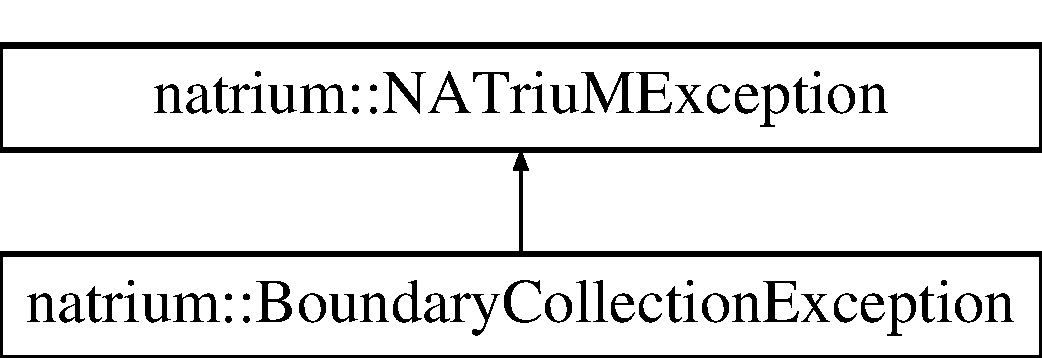
\includegraphics[height=2cm]{classnatrium_1_1BoundaryCollectionException}
\end{center}
\end{figure}
\subsection*{Public Member Functions}
\begin{DoxyCompactItemize}
\item 
\hypertarget{classnatrium_1_1BoundaryCollectionException_a287b6b5f5391b2c6457013e55f01b53e}{
{\bfseries BoundaryCollectionException} (const char $\ast$msg)}
\label{classnatrium_1_1BoundaryCollectionException_a287b6b5f5391b2c6457013e55f01b53e}

\item 
\hypertarget{classnatrium_1_1BoundaryCollectionException_a8371424ca0fa0ffb718e82df1401fde1}{
{\bfseries BoundaryCollectionException} (const string \&msg)}
\label{classnatrium_1_1BoundaryCollectionException_a8371424ca0fa0ffb718e82df1401fde1}

\item 
\hypertarget{classnatrium_1_1BoundaryCollectionException_a5e1a7fcec5fdf38baa8bd7ba8418699c}{
const char $\ast$ {\bfseries what} () const   throw ()}
\label{classnatrium_1_1BoundaryCollectionException_a5e1a7fcec5fdf38baa8bd7ba8418699c}

\end{DoxyCompactItemize}


\subsection{Detailed Description}
Exception class for Boundaries. 

The documentation for this class was generated from the following file:\begin{DoxyCompactItemize}
\item 
/mnt/fdrive/akraem3m/workspace/NATriuM/src/library/natrium/problemdescription/BoundaryCollection.h\end{DoxyCompactItemize}

\hypertarget{classnatrium_1_1BoundaryTools_1_1BoundaryDensity}{
\section{natrium::BoundaryTools::BoundaryDensity$<$ dim $>$ Class Template Reference}
\label{classnatrium_1_1BoundaryTools_1_1BoundaryDensity}\index{natrium::BoundaryTools::BoundaryDensity@{natrium::BoundaryTools::BoundaryDensity}}
}
\subsection*{Public Member Functions}
\begin{DoxyCompactItemize}
\item 
\hypertarget{classnatrium_1_1BoundaryTools_1_1BoundaryDensity_a0f8244f4ff72a645949c7baa1a430612}{
{\bfseries BoundaryDensity} (double rho=1)}
\label{classnatrium_1_1BoundaryTools_1_1BoundaryDensity_a0f8244f4ff72a645949c7baa1a430612}

\item 
\hypertarget{classnatrium_1_1BoundaryTools_1_1BoundaryDensity_a236c2f5c29f91b154beb4977e3f8c379}{
virtual double {\bfseries value} (const dealii::Point$<$ dim $>$ \&, const unsigned int=0) const }
\label{classnatrium_1_1BoundaryTools_1_1BoundaryDensity_a236c2f5c29f91b154beb4977e3f8c379}

\end{DoxyCompactItemize}
\subsubsection*{template$<$size\_\-t dim$>$ class natrium::BoundaryTools::BoundaryDensity$<$ dim $>$}



The documentation for this class was generated from the following file:\begin{DoxyCompactItemize}
\item 
/mnt/fdrive/akraem3m/workspace/NATriuM/src/library/natrium/boundaries/\hyperlink{BoundaryTools_8h}{BoundaryTools.h}\end{DoxyCompactItemize}

\hypertarget{classnatrium_1_1BoundaryTools_1_1BoundaryException}{
\section{natrium::BoundaryTools::BoundaryException Class Reference}
\label{classnatrium_1_1BoundaryTools_1_1BoundaryException}\index{natrium::BoundaryTools::BoundaryException@{natrium::BoundaryTools::BoundaryException}}
}


Exception class for Boundaries.  


{\ttfamily \#include $<$BoundaryTools.h$>$}Inheritance diagram for natrium::BoundaryTools::BoundaryException::\begin{figure}[H]
\begin{center}
\leavevmode
\includegraphics[height=2cm]{classnatrium_1_1BoundaryTools_1_1BoundaryException}
\end{center}
\end{figure}
\subsection*{Public Member Functions}
\begin{DoxyCompactItemize}
\item 
\hypertarget{classnatrium_1_1BoundaryTools_1_1BoundaryException_a9685153821678e1c219cd9c51492081a}{
{\bfseries BoundaryException} (const char $\ast$msg)}
\label{classnatrium_1_1BoundaryTools_1_1BoundaryException_a9685153821678e1c219cd9c51492081a}

\item 
\hypertarget{classnatrium_1_1BoundaryTools_1_1BoundaryException_af0004b850fab0736371aa9fdb6ff159b}{
{\bfseries BoundaryException} (const string \&msg)}
\label{classnatrium_1_1BoundaryTools_1_1BoundaryException_af0004b850fab0736371aa9fdb6ff159b}

\item 
\hypertarget{classnatrium_1_1BoundaryTools_1_1BoundaryException_ad5df14f0c881b7458db4ac3a553699bc}{
const char $\ast$ {\bfseries what} () const   throw ()}
\label{classnatrium_1_1BoundaryTools_1_1BoundaryException_ad5df14f0c881b7458db4ac3a553699bc}

\end{DoxyCompactItemize}


\subsection{Detailed Description}
Exception class for Boundaries. 

The documentation for this class was generated from the following file:\begin{DoxyCompactItemize}
\item 
/mnt/fdrive/akraem3m/workspace/NATriuM/src/library/natrium/boundaries/\hyperlink{BoundaryTools_8h}{BoundaryTools.h}\end{DoxyCompactItemize}

\hypertarget{structnatrium_1_1BoundaryHit}{
\section{natrium::BoundaryHit$<$ dim $>$ Struct Template Reference}
\label{structnatrium_1_1BoundaryHit}\index{natrium::BoundaryHit@{natrium::BoundaryHit}}
}


Defines the point in space and time where a Lagrangian path hit the boundary. \hyperlink{classnatrium_1_1Boundary}{Boundary} conditions in the Semi-\/Lagrangian LBM reconstruct the solution at the boundary hits.  


{\ttfamily \#include $<$BoundaryHit.h$>$}\subsection*{Public Member Functions}
\begin{DoxyCompactItemize}
\item 
\hypertarget{structnatrium_1_1BoundaryHit_af4c88d91789f99fced8d8d3b4cd7ebbc}{
{\bfseries BoundaryHit} (const \hyperlink{structnatrium_1_1BoundaryHit}{BoundaryHit}$<$ dim $>$ \&hit)}
\label{structnatrium_1_1BoundaryHit_af4c88d91789f99fced8d8d3b4cd7ebbc}

\item 
\hypertarget{structnatrium_1_1BoundaryHit_a2804aa93a7f03d12ec28415b42aa12ee}{
{\bfseries BoundaryHit} (const \hyperlink{structnatrium_1_1LagrangianPathTracker}{LagrangianPathTracker}$<$ dim $>$ \&tracker, const \hyperlink{classnatrium_1_1Stencil}{Stencil} \&stencil, size\_\-t boundary\_\-id, double dt\_\-global)}
\label{structnatrium_1_1BoundaryHit_a2804aa93a7f03d12ec28415b42aa12ee}

\item 
\hypertarget{structnatrium_1_1BoundaryHit_a4f20976b5fb57874538448907dbdad3d}{
size\_\-t {\bfseries getBoundaryId} () const }
\label{structnatrium_1_1BoundaryHit_a4f20976b5fb57874538448907dbdad3d}

\item 
\hypertarget{structnatrium_1_1BoundaryHit_a4ff918c172f0cb36cfc64480f68762e1}{
const dealii::Point$<$ dim $>$ \& {\bfseries getCurrentPoint} () const }
\label{structnatrium_1_1BoundaryHit_a4ff918c172f0cb36cfc64480f68762e1}

\item 
\hypertarget{structnatrium_1_1BoundaryHit_ab7467ce964ae4abd864aecabf1f9d414}{
const \hyperlink{structnatrium_1_1LagrangianPathDestination}{LagrangianPathDestination} \& {\bfseries getDestination} () const }
\label{structnatrium_1_1BoundaryHit_ab7467ce964ae4abd864aecabf1f9d414}

\item 
\hypertarget{structnatrium_1_1BoundaryHit_aa12ef41734a2e7e64e4f9cce6f517f36}{
double {\bfseries getDtHit} () const }
\label{structnatrium_1_1BoundaryHit_aa12ef41734a2e7e64e4f9cce6f517f36}

\item 
\hypertarget{structnatrium_1_1BoundaryHit_aed98a3af2ad2340721c6d4c48b3e89d8}{
const dealii::DoFHandler$<$ dim $>$::active\_\-cell\_\-iterator \& {\bfseries getCurrentCell} () const }
\label{structnatrium_1_1BoundaryHit_aed98a3af2ad2340721c6d4c48b3e89d8}

\end{DoxyCompactItemize}


\subsection{Detailed Description}
\subsubsection*{template$<$size\_\-t dim$>$ struct natrium::BoundaryHit$<$ dim $>$}

Defines the point in space and time where a Lagrangian path hit the boundary. \hyperlink{classnatrium_1_1Boundary}{Boundary} conditions in the Semi-\/Lagrangian LBM reconstruct the solution at the boundary hits. 

The documentation for this struct was generated from the following file:\begin{DoxyCompactItemize}
\item 
/mnt/fdrive/akraem3m/workspace/NATriuM/src/library/natrium/boundaries/BoundaryHit.h\end{DoxyCompactItemize}

\hypertarget{classnatrium_1_1BoundaryTools_1_1BoundaryPressure}{
\section{natrium::BoundaryTools::BoundaryPressure$<$ dim $>$ Class Template Reference}
\label{classnatrium_1_1BoundaryTools_1_1BoundaryPressure}\index{natrium::BoundaryTools::BoundaryPressure@{natrium::BoundaryTools::BoundaryPressure}}
}
\subsection*{Public Member Functions}
\begin{DoxyCompactItemize}
\item 
\hypertarget{classnatrium_1_1BoundaryTools_1_1BoundaryPressure_a0fdf874222ddfd3aba68a03b35c315ba}{
{\bfseries BoundaryPressure} (double p=0)}
\label{classnatrium_1_1BoundaryTools_1_1BoundaryPressure_a0fdf874222ddfd3aba68a03b35c315ba}

\item 
\hypertarget{classnatrium_1_1BoundaryTools_1_1BoundaryPressure_a00a51886a4b67a7b529847e911cd20c9}{
virtual double {\bfseries value} (const dealii::Point$<$ dim $>$ \&, const unsigned int=0) const }
\label{classnatrium_1_1BoundaryTools_1_1BoundaryPressure_a00a51886a4b67a7b529847e911cd20c9}

\end{DoxyCompactItemize}
\subsubsection*{template$<$size\_\-t dim$>$ class natrium::BoundaryTools::BoundaryPressure$<$ dim $>$}



The documentation for this class was generated from the following file:\begin{DoxyCompactItemize}
\item 
/mnt/fdrive/akraem3m/workspace/NATriuM/src/library/natrium/boundaries/\hyperlink{BoundaryTools_8h}{BoundaryTools.h}\end{DoxyCompactItemize}

\hypertarget{classBoundaryTestDensity}{
\section{BoundaryTestDensity Class Reference}
\label{classBoundaryTestDensity}\index{BoundaryTestDensity@{BoundaryTestDensity}}
}
\subsection*{Public Member Functions}
\begin{DoxyCompactItemize}
\item 
\hypertarget{classBoundaryTestDensity_ad53be1f68115e8645e15ee35a31f86c0}{
virtual double {\bfseries value} (const dealii::Point$<$ 2 $>$ \&, const unsigned int) const }
\label{classBoundaryTestDensity_ad53be1f68115e8645e15ee35a31f86c0}

\end{DoxyCompactItemize}


The documentation for this class was generated from the following file:\begin{DoxyCompactItemize}
\item 
/mnt/fdrive/akraem3m/workspace/NATriuM/src/test/boundaries/DirichletBoundaryRhoU2D\_\-test.cpp\end{DoxyCompactItemize}

\hypertarget{classBoundaryTestVelocity}{
\section{BoundaryTestVelocity Class Reference}
\label{classBoundaryTestVelocity}\index{BoundaryTestVelocity@{BoundaryTestVelocity}}
}
\subsection*{Public Member Functions}
\begin{DoxyCompactItemize}
\item 
\hypertarget{classBoundaryTestVelocity_a224f3ce2233b916a920ca6c6791c5d67}{
virtual void {\bfseries vector\_\-value} (const dealii::Point$<$ 2 $>$ \&, dealii::Vector$<$ double $>$ \&values) const }
\label{classBoundaryTestVelocity_a224f3ce2233b916a920ca6c6791c5d67}

\end{DoxyCompactItemize}


The documentation for this class was generated from the following file:\begin{DoxyCompactItemize}
\item 
/mnt/fdrive/akraem3m/workspace/NATriuM/src/test/boundaries/DirichletBoundaryRhoU2D\_\-test.cpp\end{DoxyCompactItemize}

\hypertarget{classnatrium_1_1BoundaryTools_1_1BoundaryVelocity}{
\section{natrium::BoundaryTools::BoundaryVelocity$<$ dim $>$ Class Template Reference}
\label{classnatrium_1_1BoundaryTools_1_1BoundaryVelocity}\index{natrium::BoundaryTools::BoundaryVelocity@{natrium::BoundaryTools::BoundaryVelocity}}
}
\subsection*{Public Member Functions}
\begin{DoxyCompactItemize}
\item 
\hypertarget{classnatrium_1_1BoundaryTools_1_1BoundaryVelocity_a0eb88d154f721f580d113ff7991a6390}{
{\bfseries BoundaryVelocity} (const dealii::Vector$<$ double $>$ \&velocity)}
\label{classnatrium_1_1BoundaryTools_1_1BoundaryVelocity_a0eb88d154f721f580d113ff7991a6390}

\item 
\hypertarget{classnatrium_1_1BoundaryTools_1_1BoundaryVelocity_adda747afd31d025b26124a038d519703}{
{\bfseries BoundaryVelocity} (const dealii::Tensor$<$ 1, dim $>$ \&velocity)}
\label{classnatrium_1_1BoundaryTools_1_1BoundaryVelocity_adda747afd31d025b26124a038d519703}

\item 
\hypertarget{classnatrium_1_1BoundaryTools_1_1BoundaryVelocity_adb91032bfd3559a43aea037c35bbf27a}{
virtual double {\bfseries value} (const dealii::Point$<$ dim $>$ \&, const unsigned int component=0) const }
\label{classnatrium_1_1BoundaryTools_1_1BoundaryVelocity_adb91032bfd3559a43aea037c35bbf27a}

\item 
\hypertarget{classnatrium_1_1BoundaryTools_1_1BoundaryVelocity_a33ffa27bf73b9749af366b9a08631905}{
virtual void {\bfseries vector\_\-value} (const dealii::Point$<$ dim $>$ \&, dealii::Vector$<$ double $>$ \&values) const }
\label{classnatrium_1_1BoundaryTools_1_1BoundaryVelocity_a33ffa27bf73b9749af366b9a08631905}

\end{DoxyCompactItemize}
\subsubsection*{template$<$size\_\-t dim$>$ class natrium::BoundaryTools::BoundaryVelocity$<$ dim $>$}



The documentation for this class was generated from the following file:\begin{DoxyCompactItemize}
\item 
/mnt/fdrive/akraem3m/workspace/NATriuM/src/library/natrium/boundaries/\hyperlink{BoundaryTools_8h}{BoundaryTools.h}\end{DoxyCompactItemize}

\hypertarget{classnatrium_1_1BoundaryTools_1_1BoundaryVelocityGradient}{
\section{natrium::BoundaryTools::BoundaryVelocityGradient$<$ dim $>$ Class Template Reference}
\label{classnatrium_1_1BoundaryTools_1_1BoundaryVelocityGradient}\index{natrium::BoundaryTools::BoundaryVelocityGradient@{natrium::BoundaryTools::BoundaryVelocityGradient}}
}
\subsection*{Public Member Functions}
\begin{DoxyCompactItemize}
\item 
\hypertarget{classnatrium_1_1BoundaryTools_1_1BoundaryVelocityGradient_af736088b755d7e64722f1af8329d45b9}{
{\bfseries BoundaryVelocityGradient} (const dealii::Tensor$<$ 2, dim $>$ \&velocity\_\-gradient)}
\label{classnatrium_1_1BoundaryTools_1_1BoundaryVelocityGradient_af736088b755d7e64722f1af8329d45b9}

\item 
\hypertarget{classnatrium_1_1BoundaryTools_1_1BoundaryVelocityGradient_a78422e38ce40181202e54509aa42354e}{
virtual dealii::Tensor$<$ 2, dim $>$ {\bfseries value} (const dealii::Point$<$ dim $>$ \&) const }
\label{classnatrium_1_1BoundaryTools_1_1BoundaryVelocityGradient_a78422e38ce40181202e54509aa42354e}

\end{DoxyCompactItemize}
\subsubsection*{template$<$size\_\-t dim$>$ class natrium::BoundaryTools::BoundaryVelocityGradient$<$ dim $>$}



The documentation for this class was generated from the following file:\begin{DoxyCompactItemize}
\item 
/mnt/fdrive/akraem3m/workspace/NATriuM/src/library/natrium/boundaries/\hyperlink{BoundaryTools_8h}{BoundaryTools.h}\end{DoxyCompactItemize}

\hypertarget{classnatrium_1_1CFDSolver}{\section{natrium\-:\-:C\-F\-D\-Solver$<$ dim $>$ Class Template Reference}
\label{classnatrium_1_1CFDSolver}\index{natrium\-::\-C\-F\-D\-Solver$<$ dim $>$@{natrium\-::\-C\-F\-D\-Solver$<$ dim $>$}}
}


The central class for the C\-F\-D simulation based on the D\-B\-E.  




{\ttfamily \#include $<$C\-F\-D\-Solver.\-h$>$}

\subsection*{Public Member Functions}
\begin{DoxyCompactItemize}
\item 
\hyperlink{classnatrium_1_1CFDSolver_a2a459e7f9d5feb0d216f869812723af2}{C\-F\-D\-Solver} (shared\-\_\-ptr$<$ \hyperlink{classnatrium_1_1SolverConfiguration}{Solver\-Configuration} $>$ configuration, shared\-\_\-ptr$<$ \hyperlink{classnatrium_1_1ProblemDescription}{Problem\-Description}$<$ dim $>$ $>$ problem\-Description)
\item 
\hypertarget{classnatrium_1_1CFDSolver_a7ca9bd709255ac87b34f869c984b913b}{virtual \hyperlink{classnatrium_1_1CFDSolver_a7ca9bd709255ac87b34f869c984b913b}{$\sim$\-C\-F\-D\-Solver} ()}\label{classnatrium_1_1CFDSolver_a7ca9bd709255ac87b34f869c984b913b}

\begin{DoxyCompactList}\small\item\em destructor \end{DoxyCompactList}\item 
\hypertarget{classnatrium_1_1CFDSolver_abe627b0bbde0635abb30b9bea4c72dc1}{void \hyperlink{classnatrium_1_1CFDSolver_abe627b0bbde0635abb30b9bea4c72dc1}{initialize\-Distributions} ()}\label{classnatrium_1_1CFDSolver_abe627b0bbde0635abb30b9bea4c72dc1}

\begin{DoxyCompactList}\small\item\em initialize distribution functions \end{DoxyCompactList}\item 
\hypertarget{classnatrium_1_1CFDSolver_ac32a318e504b31195eb61c2cdc2659fe}{void \hyperlink{classnatrium_1_1CFDSolver_ac32a318e504b31195eb61c2cdc2659fe}{stream} ()}\label{classnatrium_1_1CFDSolver_ac32a318e504b31195eb61c2cdc2659fe}

\begin{DoxyCompactList}\small\item\em Advection in all directions. \end{DoxyCompactList}\item 
\hypertarget{classnatrium_1_1CFDSolver_ac9bec7d0c4bcd5e02c5213ec09438c02}{void \hyperlink{classnatrium_1_1CFDSolver_ac9bec7d0c4bcd5e02c5213ec09438c02}{collide} ()}\label{classnatrium_1_1CFDSolver_ac9bec7d0c4bcd5e02c5213ec09438c02}

\begin{DoxyCompactList}\small\item\em Low-\/level collide function. \end{DoxyCompactList}\item 
\hypertarget{classnatrium_1_1CFDSolver_a604212a1f6cd2549b8f60ab26b14de00}{void \hyperlink{classnatrium_1_1CFDSolver_a604212a1f6cd2549b8f60ab26b14de00}{reassemble} ()}\label{classnatrium_1_1CFDSolver_a604212a1f6cd2549b8f60ab26b14de00}

\begin{DoxyCompactList}\small\item\em reassembly of all matrices \end{DoxyCompactList}\item 
\hypertarget{classnatrium_1_1CFDSolver_a11f503bc3f3c306b240874c74a38025b}{void \hyperlink{classnatrium_1_1CFDSolver_a11f503bc3f3c306b240874c74a38025b}{run} ()}\label{classnatrium_1_1CFDSolver_a11f503bc3f3c306b240874c74a38025b}

\begin{DoxyCompactList}\small\item\em run C\-F\-D solver \end{DoxyCompactList}\item 
\hypertarget{classnatrium_1_1CFDSolver_abf6804f132885502b61877fc1f9ca4a2}{void \hyperlink{classnatrium_1_1CFDSolver_abf6804f132885502b61877fc1f9ca4a2}{output} (size\-\_\-t iteration)}\label{classnatrium_1_1CFDSolver_abf6804f132885502b61877fc1f9ca4a2}

\begin{DoxyCompactList}\small\item\em create output data and write to file \end{DoxyCompactList}\item 
\hypertarget{classnatrium_1_1CFDSolver_adf0b4e4da292bcb195d926d3174ba2a9}{const distributed\-\_\-vector \& {\bfseries get\-Density} () const }\label{classnatrium_1_1CFDSolver_adf0b4e4da292bcb195d926d3174ba2a9}

\item 
\hypertarget{classnatrium_1_1CFDSolver_aa7a6591ab785a87d60bcc12da9daf8ff}{const vector\\*
$<$ distributed\-\_\-vector $>$ \& {\bfseries get\-F} () const }\label{classnatrium_1_1CFDSolver_aa7a6591ab785a87d60bcc12da9daf8ff}

\item 
\hypertarget{classnatrium_1_1CFDSolver_a0e5ec3dc278216d5827410b7db82af59}{const vector\\*
$<$ distributed\-\_\-vector $>$ \& {\bfseries get\-Velocity} () const }\label{classnatrium_1_1CFDSolver_a0e5ec3dc278216d5827410b7db82af59}

\item 
\hypertarget{classnatrium_1_1CFDSolver_a1aea207c81089c2e46092489557bb139}{const shared\-\_\-ptr\\*
$<$ \hyperlink{classnatrium_1_1AdvectionOperator}{Advection\-Operator}$<$ dim $>$ $>$ \& {\bfseries get\-Advection\-Operator} () const }\label{classnatrium_1_1CFDSolver_a1aea207c81089c2e46092489557bb139}

\item 
\hypertarget{classnatrium_1_1CFDSolver_a3733dbd256b6d38659cee3cb044c1446}{const shared\-\_\-ptr\\*
$<$ \hyperlink{classnatrium_1_1BoltzmannModel}{Boltzmann\-Model} $>$ \& {\bfseries get\-Boltzmann\-Model} () const }\label{classnatrium_1_1CFDSolver_a3733dbd256b6d38659cee3cb044c1446}

\item 
\hypertarget{classnatrium_1_1CFDSolver_abb4b632b524bd68afcdff7d54c2d3d97}{const shared\-\_\-ptr\\*
$<$ \hyperlink{classnatrium_1_1CollisionModel}{Collision\-Model} $>$ \& {\bfseries get\-Collision\-Model} () const }\label{classnatrium_1_1CFDSolver_abb4b632b524bd68afcdff7d54c2d3d97}

\item 
\hypertarget{classnatrium_1_1CFDSolver_a413691491ac82f384a03293be2294de5}{const shared\-\_\-ptr\\*
$<$ \hyperlink{classnatrium_1_1SolverConfiguration}{Solver\-Configuration} $>$ \& {\bfseries get\-Configuration} () const }\label{classnatrium_1_1CFDSolver_a413691491ac82f384a03293be2294de5}

\item 
\hypertarget{classnatrium_1_1CFDSolver_a8b1131e8fd6b022bea5ddce72469c289}{const shared\-\_\-ptr\\*
$<$ \hyperlink{classnatrium_1_1ProblemDescription}{Problem\-Description}$<$ dim $>$ $>$ \& {\bfseries get\-Problem\-Description} () const }\label{classnatrium_1_1CFDSolver_a8b1131e8fd6b022bea5ddce72469c289}

\item 
\hypertarget{classnatrium_1_1CFDSolver_adc432b8516f531639914001616d36ab9}{const shared\-\_\-ptr\\*
$<$ \hyperlink{classnatrium_1_1TimeIntegrator}{Time\-Integrator}\\*
$<$ distributed\-\_\-vector, \\*
distributed\-\_\-sparse\-\_\-matrix $>$ $>$ \& {\bfseries get\-Time\-Integrator} () const }\label{classnatrium_1_1CFDSolver_adc432b8516f531639914001616d36ab9}

\item 
\hypertarget{classnatrium_1_1CFDSolver_a74d459ef4f43d42e04ceb2178bb006f4}{size\-\_\-t {\bfseries get\-Number\-Of\-Do\-Fs} () const }\label{classnatrium_1_1CFDSolver_a74d459ef4f43d42e04ceb2178bb006f4}

\item 
\hypertarget{classnatrium_1_1CFDSolver_ae9c44bb0f33e2c73ee96fbe100061842}{double {\bfseries get\-Max\-Velocity\-Norm} () const }\label{classnatrium_1_1CFDSolver_ae9c44bb0f33e2c73ee96fbe100061842}

\item 
\hypertarget{classnatrium_1_1CFDSolver_ade641431988a82cb47d88a9d600e1c92}{double {\bfseries get\-Max\-Density\-Deviation\-From} (double reference\-Density) const }\label{classnatrium_1_1CFDSolver_ade641431988a82cb47d88a9d600e1c92}

\item 
\hypertarget{classnatrium_1_1CFDSolver_a33c4bfd63b8d457a5bc15f0c0da02c38}{size\-\_\-t {\bfseries get\-Iteration\-Start} () const }\label{classnatrium_1_1CFDSolver_a33c4bfd63b8d457a5bc15f0c0da02c38}

\end{DoxyCompactItemize}
\subsection*{Protected Member Functions}
\begin{DoxyCompactItemize}
\item 
\hypertarget{classnatrium_1_1CFDSolver_a9a2592ea549fa10427c84f0a1e380c1e}{void \hyperlink{classnatrium_1_1CFDSolver_a9a2592ea549fa10427c84f0a1e380c1e}{save\-Distribution\-Functions\-To\-Files} (const string \&directory)}\label{classnatrium_1_1CFDSolver_a9a2592ea549fa10427c84f0a1e380c1e}

\begin{DoxyCompactList}\small\item\em save the distribution functions to files for checkpointing \end{DoxyCompactList}\item 
\hypertarget{classnatrium_1_1CFDSolver_a42245d22e289d079a3b06a0c26f50050}{void \hyperlink{classnatrium_1_1CFDSolver_a42245d22e289d079a3b06a0c26f50050}{load\-Distribution\-Functions\-From\-Files} (const string \&directory)}\label{classnatrium_1_1CFDSolver_a42245d22e289d079a3b06a0c26f50050}

\begin{DoxyCompactList}\small\item\em load the distribution functions from files for checkpointing \end{DoxyCompactList}\end{DoxyCompactItemize}


\subsection{Detailed Description}
\subsubsection*{template$<$size\-\_\-t dim$>$class natrium\-::\-C\-F\-D\-Solver$<$ dim $>$}

The central class for the C\-F\-D simulation based on the D\-B\-E. 

\begin{DoxyNote}{Note}
The \hyperlink{classnatrium_1_1CFDSolver}{C\-F\-D\-Solver} itself is quite static but it contains interchangeable modules, e.\-g. for the Boltzmann model or the time integrator. By these means, a variety of different simulation methods can be covered. 
\end{DoxyNote}

\begin{DoxyTemplParams}{Template Parameters}
{\em dim} & The dimension of the flow (2 or 3). \\
\hline
\end{DoxyTemplParams}


\subsection{Constructor \& Destructor Documentation}
\hypertarget{classnatrium_1_1CFDSolver_a2a459e7f9d5feb0d216f869812723af2}{\index{natrium\-::\-C\-F\-D\-Solver@{natrium\-::\-C\-F\-D\-Solver}!C\-F\-D\-Solver@{C\-F\-D\-Solver}}
\index{C\-F\-D\-Solver@{C\-F\-D\-Solver}!natrium::CFDSolver@{natrium\-::\-C\-F\-D\-Solver}}
\subsubsection[{C\-F\-D\-Solver}]{\setlength{\rightskip}{0pt plus 5cm}template$<$size\-\_\-t dim$>$ template {\bf natrium\-::\-C\-F\-D\-Solver}$<$ dim $>$\-::{\bf C\-F\-D\-Solver} (
\begin{DoxyParamCaption}
\item[{shared\-\_\-ptr$<$ {\bf Solver\-Configuration} $>$}]{configuration, }
\item[{shared\-\_\-ptr$<$ {\bf Problem\-Description}$<$ dim $>$ $>$}]{problem\-Description}
\end{DoxyParamCaption}
)}}\label{classnatrium_1_1CFDSolver_a2a459e7f9d5feb0d216f869812723af2}
constructor \begin{DoxyNote}{Note}
\-: has to be inlined, if the template parameter is not made explicit 
\end{DoxyNote}
check if problem and solver configuration fit together

Build boltzmann model

Build streaming data object

Calculate relaxation parameter and build collision model

Build time integrator 

The documentation for this class was generated from the following files\-:\begin{DoxyCompactItemize}
\item 
/home/kraemer/eclipse\-\_\-workspace/\-N\-A\-Triu\-M/src/natrium/solver/\hyperlink{CFDSolver_8h}{C\-F\-D\-Solver.\-h}\item 
/home/kraemer/eclipse\-\_\-workspace/\-N\-A\-Triu\-M/src/natrium/solver/\hyperlink{CFDSolver_8cpp}{C\-F\-D\-Solver.\-cpp}\end{DoxyCompactItemize}

\hypertarget{classnatrium_1_1CFDSolverException}{
\section{natrium::CFDSolverException Class Reference}
\label{classnatrium_1_1CFDSolverException}\index{natrium::CFDSolverException@{natrium::CFDSolverException}}
}


Exception class for \hyperlink{classnatrium_1_1CFDSolver}{CFDSolver}.  


{\ttfamily \#include $<$CFDSolver.h$>$}Inheritance diagram for natrium::CFDSolverException::\begin{figure}[H]
\begin{center}
\leavevmode
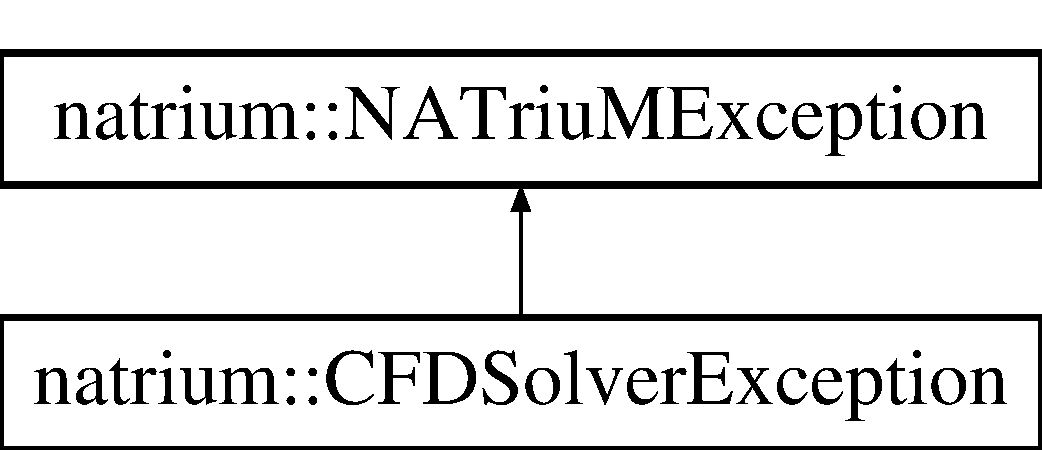
\includegraphics[height=2cm]{classnatrium_1_1CFDSolverException}
\end{center}
\end{figure}
\subsection*{Public Member Functions}
\begin{DoxyCompactItemize}
\item 
\hypertarget{classnatrium_1_1CFDSolverException_a1256570132b679d57fe046f648656051}{
{\bfseries CFDSolverException} (const char $\ast$msg)}
\label{classnatrium_1_1CFDSolverException_a1256570132b679d57fe046f648656051}

\item 
\hypertarget{classnatrium_1_1CFDSolverException_a1fc20604a6925cd3577fe3fa7c0f585e}{
{\bfseries CFDSolverException} (const string \&msg)}
\label{classnatrium_1_1CFDSolverException_a1fc20604a6925cd3577fe3fa7c0f585e}

\item 
\hypertarget{classnatrium_1_1CFDSolverException_ae1e5d3d088b808ab4c995d1209a86a1f}{
const char $\ast$ {\bfseries what} () const   throw ()}
\label{classnatrium_1_1CFDSolverException_ae1e5d3d088b808ab4c995d1209a86a1f}

\end{DoxyCompactItemize}


\subsection{Detailed Description}
Exception class for \hyperlink{classnatrium_1_1CFDSolver}{CFDSolver}. 

The documentation for this class was generated from the following file:\begin{DoxyCompactItemize}
\item 
/mnt/fdrive/akraem3m/workspace/NATriuM/src/library/natrium/solver/\hyperlink{CFDSolver_8h}{CFDSolver.h}\end{DoxyCompactItemize}

\hypertarget{classnatrium_1_1CFDSolverUtilities_1_1CFDSolverUtilitiesException}{
\section{natrium::CFDSolverUtilities::CFDSolverUtilitiesException Class Reference}
\label{classnatrium_1_1CFDSolverUtilities_1_1CFDSolverUtilitiesException}\index{natrium::CFDSolverUtilities::CFDSolverUtilitiesException@{natrium::CFDSolverUtilities::CFDSolverUtilitiesException}}
}
Inheritance diagram for natrium::CFDSolverUtilities::CFDSolverUtilitiesException::\begin{figure}[H]
\begin{center}
\leavevmode
\includegraphics[height=2cm]{classnatrium_1_1CFDSolverUtilities_1_1CFDSolverUtilitiesException}
\end{center}
\end{figure}
\subsection*{Public Member Functions}
\begin{DoxyCompactItemize}
\item 
\hypertarget{classnatrium_1_1CFDSolverUtilities_1_1CFDSolverUtilitiesException_a19add4b16c155613f9d8a2fc72bbeca9}{
{\bfseries CFDSolverUtilitiesException} (const char $\ast$msg)}
\label{classnatrium_1_1CFDSolverUtilities_1_1CFDSolverUtilitiesException_a19add4b16c155613f9d8a2fc72bbeca9}

\item 
\hypertarget{classnatrium_1_1CFDSolverUtilities_1_1CFDSolverUtilitiesException_acf6fcdce9460af595b457d6830353d9d}{
{\bfseries CFDSolverUtilitiesException} (const string \&msg)}
\label{classnatrium_1_1CFDSolverUtilities_1_1CFDSolverUtilitiesException_acf6fcdce9460af595b457d6830353d9d}

\item 
\hypertarget{classnatrium_1_1CFDSolverUtilities_1_1CFDSolverUtilitiesException_a548a8cb9bd2c52753a7c334836ae9865}{
const char $\ast$ {\bfseries what} () const   throw ()}
\label{classnatrium_1_1CFDSolverUtilities_1_1CFDSolverUtilitiesException_a548a8cb9bd2c52753a7c334836ae9865}

\end{DoxyCompactItemize}


The documentation for this class was generated from the following file:\begin{DoxyCompactItemize}
\item 
/mnt/fdrive/akraem3m/workspace/NATriuM/src/library/natrium/utilities/\hyperlink{CFDSolverUtilities_8h}{CFDSolverUtilities.h}\end{DoxyCompactItemize}

\hypertarget{classnatrium_1_1Checkpoint}{
\section{natrium::Checkpoint$<$ dim $>$ Class Template Reference}
\label{classnatrium_1_1Checkpoint}\index{natrium::Checkpoint@{natrium::Checkpoint}}
}


A class describing the checkpoint.  


{\ttfamily \#include $<$Checkpoint.h$>$}\subsection*{Public Member Functions}
\begin{DoxyCompactItemize}
\item 
\hyperlink{classnatrium_1_1Checkpoint_a8d5798dea2e38acce751dd1194d76c27}{Checkpoint} (size\_\-t iteration, boost::filesystem::path checkpoint\_\-dir)
\begin{DoxyCompactList}\small\item\em Constructor. \item\end{DoxyCompactList}\item 
bool \hyperlink{classnatrium_1_1Checkpoint_a43f7d305056ef5eab7a2efea2cdaebe5}{exists} ()
\begin{DoxyCompactList}\small\item\em Function that determines whether the checkpoint files exist. \item\end{DoxyCompactList}\item 
\hypertarget{classnatrium_1_1Checkpoint_a6c3eae90337f91948b4b17ad2456258c}{
void \hyperlink{classnatrium_1_1Checkpoint_a6c3eae90337f91948b4b17ad2456258c}{write} (const Mesh$<$ dim $>$ \&mesh, const \hyperlink{classnatrium_1_1DistributionFunctions}{DistributionFunctions} \&f, const dealii::DoFHandler$<$ dim $>$ \&dof\_\-handler, const \hyperlink{structnatrium_1_1CheckpointStatus}{CheckpointStatus} \&status)}
\label{classnatrium_1_1Checkpoint_a6c3eae90337f91948b4b17ad2456258c}

\begin{DoxyCompactList}\small\item\em Write checkpoint to checkpoint directory. A checkpoint contains of three files:
\begin{DoxyEnumerate}
\item a .stat file that contains some information about the status of the simulations (iteration number, time, stencil scaling, ...).
\item a .data file that contains the serialized data (mesh and distribution functions)
\item a .data.info file that contains some deal.II information about the mesh, refinement etc. 
\end{DoxyEnumerate}\item\end{DoxyCompactList}\item 
\hypertarget{classnatrium_1_1Checkpoint_a71c6fb7d10a93b2dedc981fb9cdbb488}{
void \hyperlink{classnatrium_1_1Checkpoint_a71c6fb7d10a93b2dedc981fb9cdbb488}{load} (\hyperlink{classnatrium_1_1DistributionFunctions}{DistributionFunctions} \&f, \hyperlink{classnatrium_1_1ProblemDescription}{ProblemDescription}$<$ dim $>$ \&problem, \hyperlink{classnatrium_1_1AdvectionOperator}{AdvectionOperator}$<$ dim $>$ \&advection, \hyperlink{structnatrium_1_1CheckpointStatus}{CheckpointStatus} \&status)}
\label{classnatrium_1_1Checkpoint_a71c6fb7d10a93b2dedc981fb9cdbb488}

\begin{DoxyCompactList}\small\item\em Load checkpoint from file. A simulation can be resumed from a checkpoint if
\begin{DoxyEnumerate}
\item the mesh is exactly the same as in the previous simulation
\item the mesh is a globally refined version of the previous simulation Restarts are also possible with arbitrary Mach number. Varying the order of finite elements is not supported, so far. 
\end{DoxyEnumerate}\item\end{DoxyCompactList}\item 
\hypertarget{classnatrium_1_1Checkpoint_a8391abf13cccdac1c3f2ad1ec4596541}{
const boost::filesystem::path \& {\bfseries getDataFile} () const }
\label{classnatrium_1_1Checkpoint_a8391abf13cccdac1c3f2ad1ec4596541}

\item 
\hypertarget{classnatrium_1_1Checkpoint_af2b2fe54ca03a86df627f10848df98c8}{
const boost::filesystem::path \& {\bfseries getStatusFile} () const }
\label{classnatrium_1_1Checkpoint_af2b2fe54ca03a86df627f10848df98c8}

\end{DoxyCompactItemize}
\subsection*{Static Public Member Functions}
\begin{DoxyCompactItemize}
\item 
\hypertarget{classnatrium_1_1Checkpoint_a8ab0b57861be8c348efbe20bc5dec303}{
static void {\bfseries loadFromDeprecatedCheckpointVersion} (\hyperlink{classnatrium_1_1DistributionFunctions}{DistributionFunctions} \&f, \hyperlink{classnatrium_1_1AdvectionOperator}{AdvectionOperator}$<$ dim $>$ \&advection, string directory, \hyperlink{structnatrium_1_1CheckpointStatus}{CheckpointStatus} \&status)}
\label{classnatrium_1_1Checkpoint_a8ab0b57861be8c348efbe20bc5dec303}

\end{DoxyCompactItemize}


\subsection{Detailed Description}
\subsubsection*{template$<$size\_\-t dim$>$ class natrium::Checkpoint$<$ dim $>$}

A class describing the checkpoint. 

\subsection{Constructor \& Destructor Documentation}
\hypertarget{classnatrium_1_1Checkpoint_a8d5798dea2e38acce751dd1194d76c27}{
\index{natrium::Checkpoint@{natrium::Checkpoint}!Checkpoint@{Checkpoint}}
\index{Checkpoint@{Checkpoint}!natrium::Checkpoint@{natrium::Checkpoint}}
\subsubsection[{Checkpoint}]{\setlength{\rightskip}{0pt plus 5cm}template$<$size\_\-t dim$>$ {\bf natrium::Checkpoint}$<$ dim $>$::{\bf Checkpoint} (size\_\-t {\em iteration}, \/  boost::filesystem::path {\em checkpoint\_\-dir})\hspace{0.3cm}{\ttfamily  \mbox{[}inline\mbox{]}}}}
\label{classnatrium_1_1Checkpoint_a8d5798dea2e38acce751dd1194d76c27}


Constructor. 
\begin{DoxyParams}{Parameters}
\item[\mbox{$\leftarrow$} {\em iteration}]The iteration number of the checkpoint (save or load). \item[\mbox{$\leftarrow$} {\em checkpoint\_\-dir}]The directory in which the checkpoint was saved. \end{DoxyParams}


\subsection{Member Function Documentation}
\hypertarget{classnatrium_1_1Checkpoint_a43f7d305056ef5eab7a2efea2cdaebe5}{
\index{natrium::Checkpoint@{natrium::Checkpoint}!exists@{exists}}
\index{exists@{exists}!natrium::Checkpoint@{natrium::Checkpoint}}
\subsubsection[{exists}]{\setlength{\rightskip}{0pt plus 5cm}template$<$size\_\-t dim$>$ bool {\bf natrium::Checkpoint}$<$ dim $>$::exists ()\hspace{0.3cm}{\ttfamily  \mbox{[}inline\mbox{]}}}}
\label{classnatrium_1_1Checkpoint_a43f7d305056ef5eab7a2efea2cdaebe5}


Function that determines whether the checkpoint files exist. \begin{DoxyReturn}{Returns}
boolean 
\end{DoxyReturn}


The documentation for this class was generated from the following files:\begin{DoxyCompactItemize}
\item 
/mnt/fdrive/akraem3m/workspace/NATriuM/src/library/natrium/solver/Checkpoint.h\item 
/mnt/fdrive/akraem3m/workspace/NATriuM/src/library/natrium/solver/Checkpoint.cpp\end{DoxyCompactItemize}

\hypertarget{classnatrium_1_1CheckpointException}{
\section{natrium::CheckpointException Class Reference}
\label{classnatrium_1_1CheckpointException}\index{natrium::CheckpointException@{natrium::CheckpointException}}
}


Exception class for \hyperlink{classnatrium_1_1CFDSolver}{CFDSolver}.  


{\ttfamily \#include $<$Checkpoint.h$>$}Inheritance diagram for natrium::CheckpointException::\begin{figure}[H]
\begin{center}
\leavevmode
\includegraphics[height=2cm]{classnatrium_1_1CheckpointException}
\end{center}
\end{figure}
\subsection*{Public Member Functions}
\begin{DoxyCompactItemize}
\item 
\hypertarget{classnatrium_1_1CheckpointException_ae290a3ee4789a56b69561f6d339be0fa}{
{\bfseries CheckpointException} (const char $\ast$msg)}
\label{classnatrium_1_1CheckpointException_ae290a3ee4789a56b69561f6d339be0fa}

\item 
\hypertarget{classnatrium_1_1CheckpointException_a821774598aa17b83c0fd126677b42019}{
{\bfseries CheckpointException} (const string \&msg)}
\label{classnatrium_1_1CheckpointException_a821774598aa17b83c0fd126677b42019}

\item 
\hypertarget{classnatrium_1_1CheckpointException_a47b6dca60268391fbbf2ab359129396c}{
const char $\ast$ {\bfseries what} () const   throw ()}
\label{classnatrium_1_1CheckpointException_a47b6dca60268391fbbf2ab359129396c}

\end{DoxyCompactItemize}


\subsection{Detailed Description}
Exception class for \hyperlink{classnatrium_1_1CFDSolver}{CFDSolver}. 

The documentation for this class was generated from the following file:\begin{DoxyCompactItemize}
\item 
/mnt/fdrive/akraem3m/workspace/NATriuM/src/library/natrium/solver/Checkpoint.h\end{DoxyCompactItemize}

\hypertarget{structnatrium_1_1CheckpointStatus}{
\section{natrium::CheckpointStatus Struct Reference}
\label{structnatrium_1_1CheckpointStatus}\index{natrium::CheckpointStatus@{natrium::CheckpointStatus}}
}


A struct describing the status of a checkpoint (iteration number, time, stencil scaling).  


{\ttfamily \#include $<$Checkpoint.h$>$}\subsection*{Public Attributes}
\begin{DoxyCompactItemize}
\item 
\hypertarget{structnatrium_1_1CheckpointStatus_add611ef5de19fbe01990fd5fabf855e0}{
double {\bfseries time}}
\label{structnatrium_1_1CheckpointStatus_add611ef5de19fbe01990fd5fabf855e0}

\item 
\hypertarget{structnatrium_1_1CheckpointStatus_ac8a23227bdb13573d304582d7db9e6f2}{
size\_\-t {\bfseries iterationNumber}}
\label{structnatrium_1_1CheckpointStatus_ac8a23227bdb13573d304582d7db9e6f2}

\item 
\hypertarget{structnatrium_1_1CheckpointStatus_af4691a7ffd4070ea987742c5837ba7b0}{
double {\bfseries stencilScaling}}
\label{structnatrium_1_1CheckpointStatus_af4691a7ffd4070ea987742c5837ba7b0}

\item 
\hypertarget{structnatrium_1_1CheckpointStatus_a5fd25fdb804d466d7e985dd2197b5c12}{
size\_\-t {\bfseries feOrder}}
\label{structnatrium_1_1CheckpointStatus_a5fd25fdb804d466d7e985dd2197b5c12}

\end{DoxyCompactItemize}


\subsection{Detailed Description}
A struct describing the status of a checkpoint (iteration number, time, stencil scaling). 

The documentation for this struct was generated from the following file:\begin{DoxyCompactItemize}
\item 
/mnt/fdrive/akraem3m/workspace/NATriuM/src/library/natrium/solver/Checkpoint.h\end{DoxyCompactItemize}

\hypertarget{classnatrium_1_1CollisionException}{
\section{natrium::CollisionException Class Reference}
\label{classnatrium_1_1CollisionException}\index{natrium::CollisionException@{natrium::CollisionException}}
}


Exception class for Collision.  


{\ttfamily \#include $<$CollisionModel.h$>$}Inheritance diagram for natrium::CollisionException::\begin{figure}[H]
\begin{center}
\leavevmode
\includegraphics[height=2cm]{classnatrium_1_1CollisionException}
\end{center}
\end{figure}
\subsection*{Public Member Functions}
\begin{DoxyCompactItemize}
\item 
\hypertarget{classnatrium_1_1CollisionException_aee60989a43066bd65b0481cde4d96980}{
{\bfseries CollisionException} (const char $\ast$msg)}
\label{classnatrium_1_1CollisionException_aee60989a43066bd65b0481cde4d96980}

\item 
\hypertarget{classnatrium_1_1CollisionException_a36cefc1d84dec3d981a84250de56aca1}{
{\bfseries CollisionException} (const string \&msg)}
\label{classnatrium_1_1CollisionException_a36cefc1d84dec3d981a84250de56aca1}

\item 
\hypertarget{classnatrium_1_1CollisionException_a700f9ee10ef668a35cb227d8a7b01d4c}{
const char $\ast$ {\bfseries what} () const   throw ()}
\label{classnatrium_1_1CollisionException_a700f9ee10ef668a35cb227d8a7b01d4c}

\end{DoxyCompactItemize}


\subsection{Detailed Description}
Exception class for Collision. 

The documentation for this class was generated from the following file:\begin{DoxyCompactItemize}
\item 
/mnt/fdrive/akraem3m/workspace/NATriuM/src/library/natrium/collision/\hyperlink{CollisionModel_8h}{CollisionModel.h}\end{DoxyCompactItemize}

\hypertarget{classnatrium_1_1CollisionModel}{
\section{natrium::CollisionModel Class Reference}
\label{classnatrium_1_1CollisionModel}\index{natrium::CollisionModel@{natrium::CollisionModel}}
}


Abstract collision model. Required to have a common parent of all template specializations of Collision.  


{\ttfamily \#include $<$CollisionModel.h$>$}Inheritance diagram for natrium::CollisionModel::\begin{figure}[H]
\begin{center}
\leavevmode
\includegraphics[height=5cm]{classnatrium_1_1CollisionModel}
\end{center}
\end{figure}
\subsection*{Public Member Functions}
\begin{DoxyCompactItemize}
\item 
\hypertarget{classnatrium_1_1CollisionModel_a443734919886ea5880be3bba1257758d}{
{\bfseries CollisionModel} (const boost::shared\_\-ptr$<$ \hyperlink{classnatrium_1_1Stencil}{Stencil} $>$ stencil, ForceType force\_\-type=NO\_\-FORCING)}
\label{classnatrium_1_1CollisionModel_a443734919886ea5880be3bba1257758d}

\item 
\hypertarget{classnatrium_1_1CollisionModel_ac6c6d95633d62209a04528af86807025}{
virtual void {\bfseries collideAll} (\hyperlink{classnatrium_1_1DistributionFunctions}{DistributionFunctions} \&f, \hyperlink{namespacenatrium_a903d2b92917f582f2ff05f52160ab811}{distributed\_\-vector} \&densities, vector$<$ \hyperlink{namespacenatrium_a903d2b92917f582f2ff05f52160ab811}{distributed\_\-vector} $>$ \&velocities, const dealii::IndexSet \&locally\_\-owned\_\-dofs, bool inInitializationProcedure=false) const =0}
\label{classnatrium_1_1CollisionModel_ac6c6d95633d62209a04528af86807025}

\item 
\hypertarget{classnatrium_1_1CollisionModel_ab1ec1368662524bb87006f9038b4972d}{
virtual void {\bfseries setTimeStep} (double dt)}
\label{classnatrium_1_1CollisionModel_ab1ec1368662524bb87006f9038b4972d}

\item 
\hypertarget{classnatrium_1_1CollisionModel_ac10edd12e081a6eb48a36568f1bc1c0f}{
const boost::shared\_\-ptr$<$ \hyperlink{classnatrium_1_1Stencil}{Stencil} $>$ \& {\bfseries getStencil} () const }
\label{classnatrium_1_1CollisionModel_ac10edd12e081a6eb48a36568f1bc1c0f}

\item 
virtual double \hyperlink{classnatrium_1_1CollisionModel_ae1c879c87ac210a227a8e3da2d0ac385}{calculateDensity} (const vector$<$ double $>$ \&distributions) const 
\begin{DoxyCompactList}\small\item\em calculate macroscopic density \item\end{DoxyCompactList}\item 
virtual \hyperlink{namespacenatrium_a67c39077adc6634f8fa3762b8eef24c4}{numeric\_\-vector} \hyperlink{classnatrium_1_1CollisionModel_a90428f4c29916641de3de872803dde0f}{calculateVelocity} (const vector$<$ double $>$ \&distributions) const 
\begin{DoxyCompactList}\small\item\em calculate macroscopic velocity \item\end{DoxyCompactList}\item 
virtual void \hyperlink{classnatrium_1_1CollisionModel_a667f0e36da1bfb1c5102adb8f3afdcde}{calculateVelocity} (const vector$<$ double $>$ \&distributions, const double rho, \hyperlink{namespacenatrium_a67c39077adc6634f8fa3762b8eef24c4}{numeric\_\-vector} \&u) const 
\begin{DoxyCompactList}\small\item\em calculate macroscopic velocity; saves the double calculation of the density \item\end{DoxyCompactList}\item 
virtual double \hyperlink{classnatrium_1_1CollisionModel_a88b382d63da80e950bc58e8afad769a6}{getEquilibriumDistribution} (size\_\-t i, const \hyperlink{namespacenatrium_a67c39077adc6634f8fa3762b8eef24c4}{numeric\_\-vector} \&u, const double rho=1) const =0
\begin{DoxyCompactList}\small\item\em virtual function for the calculation of the equilibrium distribution \item\end{DoxyCompactList}\item 
virtual void \hyperlink{classnatrium_1_1CollisionModel_a296474961c4501bc23228be1d30ebf82}{getEquilibriumDistributions} (vector$<$ double $>$ \&feq, const \hyperlink{namespacenatrium_a67c39077adc6634f8fa3762b8eef24c4}{numeric\_\-vector} \&u, const double rho=1) const 
\begin{DoxyCompactList}\small\item\em function for the calculation of all equilibrium distributions \item\end{DoxyCompactList}\item 
\hypertarget{classnatrium_1_1CollisionModel_a44bababd58cae1fea650fe2bd86555b5}{
void {\bfseries setExternalForce} (const \hyperlink{classnatrium_1_1ConstantExternalForce}{ConstantExternalForce}$<$ 2 $>$ \&external\_\-force)}
\label{classnatrium_1_1CollisionModel_a44bababd58cae1fea650fe2bd86555b5}

\item 
\hypertarget{classnatrium_1_1CollisionModel_ae899a80c7dcfbbdb68dd6b4e4fff5a49}{
void {\bfseries setExternalForce} (const \hyperlink{classnatrium_1_1ConstantExternalForce}{ConstantExternalForce}$<$ 3 $>$ \&external\_\-force)}
\label{classnatrium_1_1CollisionModel_ae899a80c7dcfbbdb68dd6b4e4fff5a49}

\item 
\hypertarget{classnatrium_1_1CollisionModel_a6806e1494a2bbb03c27b146261af408b}{
ForceType {\bfseries getForceType} () const }
\label{classnatrium_1_1CollisionModel_a6806e1494a2bbb03c27b146261af408b}

\item 
\hypertarget{classnatrium_1_1CollisionModel_a366ae27de1bf045fd9bf0159e251054a}{
double {\bfseries getForceX} () const }
\label{classnatrium_1_1CollisionModel_a366ae27de1bf045fd9bf0159e251054a}

\item 
\hypertarget{classnatrium_1_1CollisionModel_a1282b42d5c270b9f031def96dbe15866}{
double {\bfseries getForceY} () const }
\label{classnatrium_1_1CollisionModel_a1282b42d5c270b9f031def96dbe15866}

\item 
\hypertarget{classnatrium_1_1CollisionModel_a60fa9f8c1614789027c553264524fb5e}{
double {\bfseries getForceZ} () const }
\label{classnatrium_1_1CollisionModel_a60fa9f8c1614789027c553264524fb5e}

\item 
\hypertarget{classnatrium_1_1CollisionModel_acff518f0353a95dfbf3ddeba2a7ed7f6}{
void {\bfseries setForceType} (ForceType forceType)}
\label{classnatrium_1_1CollisionModel_acff518f0353a95dfbf3ddeba2a7ed7f6}

\item 
\hypertarget{classnatrium_1_1CollisionModel_aa2a154a99039deb620501ef2e525089f}{
double {\bfseries getTimeStep} () const }
\label{classnatrium_1_1CollisionModel_aa2a154a99039deb620501ef2e525089f}

\item 
\hypertarget{classnatrium_1_1CollisionModel_a4ee445caf75fff704811e29fc46f431e}{
double {\bfseries getViscosity} () const }
\label{classnatrium_1_1CollisionModel_a4ee445caf75fff704811e29fc46f431e}

\item 
\hypertarget{classnatrium_1_1CollisionModel_a43cfd1efe035afb6f170b7b05c18113a}{
void {\bfseries setViscosity} (double viscosity)}
\label{classnatrium_1_1CollisionModel_a43cfd1efe035afb6f170b7b05c18113a}

\end{DoxyCompactItemize}


\subsection{Detailed Description}
Abstract collision model. Required to have a common parent of all template specializations of Collision. 

\subsection{Member Function Documentation}
\hypertarget{classnatrium_1_1CollisionModel_ae1c879c87ac210a227a8e3da2d0ac385}{
\index{natrium::CollisionModel@{natrium::CollisionModel}!calculateDensity@{calculateDensity}}
\index{calculateDensity@{calculateDensity}!natrium::CollisionModel@{natrium::CollisionModel}}
\subsubsection[{calculateDensity}]{\setlength{\rightskip}{0pt plus 5cm}virtual double natrium::CollisionModel::calculateDensity (const vector$<$ double $>$ \& {\em distributions}) const\hspace{0.3cm}{\ttfamily  \mbox{[}inline, virtual\mbox{]}}}}
\label{classnatrium_1_1CollisionModel_ae1c879c87ac210a227a8e3da2d0ac385}


calculate macroscopic density 
\begin{DoxyParams}{Parameters}
\item[\mbox{$\leftarrow$} {\em distributions}]particle distribution functions at a given point \end{DoxyParams}
\begin{DoxyReturn}{Returns}
macroscopic density (sum of all distributions) 
\end{DoxyReturn}


Reimplemented in \hyperlink{classnatrium_1_1BGKStandardTransformed_a58c4dc0c67ff4898c6555b614afc1ace}{natrium::BGKStandardTransformed}.\hypertarget{classnatrium_1_1CollisionModel_a667f0e36da1bfb1c5102adb8f3afdcde}{
\index{natrium::CollisionModel@{natrium::CollisionModel}!calculateVelocity@{calculateVelocity}}
\index{calculateVelocity@{calculateVelocity}!natrium::CollisionModel@{natrium::CollisionModel}}
\subsubsection[{calculateVelocity}]{\setlength{\rightskip}{0pt plus 5cm}virtual void natrium::CollisionModel::calculateVelocity (const vector$<$ double $>$ \& {\em distributions}, \/  const double {\em rho}, \/  {\bf numeric\_\-vector} \& {\em u}) const\hspace{0.3cm}{\ttfamily  \mbox{[}inline, virtual\mbox{]}}}}
\label{classnatrium_1_1CollisionModel_a667f0e36da1bfb1c5102adb8f3afdcde}


calculate macroscopic velocity; saves the double calculation of the density \begin{DoxyNote}{Note}
more efficient 
\end{DoxyNote}

\begin{DoxyParams}{Parameters}
\item[\mbox{$\leftarrow$} {\em distributions}]particle distribution functions at a given point \item[\mbox{$\leftarrow$} {\em rho}]macroscopic density \item[\mbox{$\rightarrow$} {\em u}]macroscopic velocity \end{DoxyParams}
\hypertarget{classnatrium_1_1CollisionModel_a90428f4c29916641de3de872803dde0f}{
\index{natrium::CollisionModel@{natrium::CollisionModel}!calculateVelocity@{calculateVelocity}}
\index{calculateVelocity@{calculateVelocity}!natrium::CollisionModel@{natrium::CollisionModel}}
\subsubsection[{calculateVelocity}]{\setlength{\rightskip}{0pt plus 5cm}virtual {\bf numeric\_\-vector} natrium::CollisionModel::calculateVelocity (const vector$<$ double $>$ \& {\em distributions}) const\hspace{0.3cm}{\ttfamily  \mbox{[}inline, virtual\mbox{]}}}}
\label{classnatrium_1_1CollisionModel_a90428f4c29916641de3de872803dde0f}


calculate macroscopic velocity 
\begin{DoxyParams}{Parameters}
\item[\mbox{$\leftarrow$} {\em distributions}]particle distribution functions at a given point \end{DoxyParams}
\begin{DoxyReturn}{Returns}
macroscopic velocity 
\end{DoxyReturn}
\hypertarget{classnatrium_1_1CollisionModel_a88b382d63da80e950bc58e8afad769a6}{
\index{natrium::CollisionModel@{natrium::CollisionModel}!getEquilibriumDistribution@{getEquilibriumDistribution}}
\index{getEquilibriumDistribution@{getEquilibriumDistribution}!natrium::CollisionModel@{natrium::CollisionModel}}
\subsubsection[{getEquilibriumDistribution}]{\setlength{\rightskip}{0pt plus 5cm}virtual double natrium::CollisionModel::getEquilibriumDistribution (size\_\-t {\em i}, \/  const {\bf numeric\_\-vector} \& {\em u}, \/  const double {\em rho} = {\ttfamily 1}) const\hspace{0.3cm}{\ttfamily  \mbox{[}pure virtual\mbox{]}}}}
\label{classnatrium_1_1CollisionModel_a88b382d63da80e950bc58e8afad769a6}


virtual function for the calculation of the equilibrium distribution 
\begin{DoxyParams}{Parameters}
\item[{\em i}]index of the direction \item[{\em u}]macroscopic velocity \item[{\em rho}]macroscopic density \end{DoxyParams}
\begin{DoxyReturn}{Returns}
value of the equilibrium distribution 
\end{DoxyReturn}
\begin{DoxyNote}{Note}
The calculation can surely be done more efficiently by passing different arguments, e.g. u$\ast$u or u/(c$^\wedge$2) 
\end{DoxyNote}


Implemented in \hyperlink{classnatrium_1_1BGKIncompressible_a26dd8954261b04f8383ca9d37f5ac8c0}{natrium::BGKIncompressible}, \hyperlink{classnatrium_1_1BGKMultistep_a034cd475974bcce0db64e52245efd91d}{natrium::BGKMultistep}, \hyperlink{classnatrium_1_1BGKPseudopotential_a366ccd417ca4ad5fa37ce0572e0d6fe4}{natrium::BGKPseudopotential$<$ dim $>$}, \hyperlink{classnatrium_1_1BGKStandard_a3d45ef2fe5536bf14914f99297477754}{natrium::BGKStandard}, \hyperlink{classnatrium_1_1BGKStandardTransformed_a870465cc026f92c8ffba899af6f95634}{natrium::BGKStandardTransformed}, \hyperlink{classnatrium_1_1BGKSteadyState_ad99d9159cc14b5897bea7f145c3b39ca}{natrium::BGKSteadyState}, \hyperlink{classnatrium_1_1KBCStandard_a1dac2deaafb93027bf168887dd2e002d}{natrium::KBCStandard}, and \hyperlink{classnatrium_1_1MRT_a3f96915f9f67680f4a1d7b952e70be55}{natrium::MRT}.\hypertarget{classnatrium_1_1CollisionModel_a296474961c4501bc23228be1d30ebf82}{
\index{natrium::CollisionModel@{natrium::CollisionModel}!getEquilibriumDistributions@{getEquilibriumDistributions}}
\index{getEquilibriumDistributions@{getEquilibriumDistributions}!natrium::CollisionModel@{natrium::CollisionModel}}
\subsubsection[{getEquilibriumDistributions}]{\setlength{\rightskip}{0pt plus 5cm}void natrium::CollisionModel::getEquilibriumDistributions (vector$<$ double $>$ \& {\em feq}, \/  const {\bf numeric\_\-vector} \& {\em u}, \/  const double {\em rho} = {\ttfamily 1}) const\hspace{0.3cm}{\ttfamily  \mbox{[}virtual\mbox{]}}}}
\label{classnatrium_1_1CollisionModel_a296474961c4501bc23228be1d30ebf82}


function for the calculation of all equilibrium distributions 
\begin{DoxyParams}{Parameters}
\item[\mbox{$\rightarrow$} {\em feq}]vector of all equality distributions, must have size Q \item[\mbox{$\leftarrow$} {\em u}]macroscopic velocity \item[\mbox{$\leftarrow$} {\em rho}]macroscopic density \end{DoxyParams}
\begin{DoxyNote}{Note}
The calculation can surely be done more efficiently by passing different arguments, e.g. u$\ast$u or u/(c$^\wedge$2) 
\end{DoxyNote}


The documentation for this class was generated from the following files:\begin{DoxyCompactItemize}
\item 
/mnt/fdrive/akraem3m/workspace/NATriuM/src/library/natrium/collision/\hyperlink{CollisionModel_8h}{CollisionModel.h}\item 
/mnt/fdrive/akraem3m/workspace/NATriuM/src/library/natrium/collision/\hyperlink{CollisionModel_8cpp}{CollisionModel.cpp}\end{DoxyCompactItemize}

\hypertarget{classnatrium_1_1CompareToBotella}{
\section{natrium::CompareToBotella Class Reference}
\label{classnatrium_1_1CompareToBotella}\index{natrium::CompareToBotella@{natrium::CompareToBotella}}
}
Inheritance diagram for natrium::CompareToBotella::\begin{figure}[H]
\begin{center}
\leavevmode
\includegraphics[height=2cm]{classnatrium_1_1CompareToBotella}
\end{center}
\end{figure}
\subsection*{Public Member Functions}
\begin{DoxyCompactItemize}
\item 
\hypertarget{classnatrium_1_1CompareToBotella_ad525363c302f82cd7cd24ae2b58130f8}{
{\bfseries CompareToBotella} (const \hyperlink{classnatrium_1_1CFDSolver}{CFDSolver}$<$ 2 $>$ \&solver, size\_\-t reynolds, string filename)}
\label{classnatrium_1_1CompareToBotella_ad525363c302f82cd7cd24ae2b58130f8}

\item 
\hypertarget{classnatrium_1_1CompareToBotella_a5b9c9fc30b852aa7898a955bf0ef10ff}{
void {\bfseries makeReferenceU} (\hyperlink{namespacenatrium_a67c39077adc6634f8fa3762b8eef24c4}{numeric\_\-vector} \&u, size\_\-t reynolds\_\-number)}
\label{classnatrium_1_1CompareToBotella_a5b9c9fc30b852aa7898a955bf0ef10ff}

\item 
\hypertarget{classnatrium_1_1CompareToBotella_a03a64dd371a6fc0c49d746b42eda001f}{
void {\bfseries makeReferenceV} (\hyperlink{namespacenatrium_a67c39077adc6634f8fa3762b8eef24c4}{numeric\_\-vector} \&v, size\_\-t reynolds\_\-number)}
\label{classnatrium_1_1CompareToBotella_a03a64dd371a6fc0c49d746b42eda001f}

\item 
\hypertarget{classnatrium_1_1CompareToBotella_aabd82dd44d264d2c371036c4c6b1feac}{
virtual void {\bfseries apply} ()}
\label{classnatrium_1_1CompareToBotella_aabd82dd44d264d2c371036c4c6b1feac}

\item 
\hypertarget{classnatrium_1_1CompareToBotella_ae85f948147a9926193c0b0cafdf37132}{
void {\bfseries printFinalVelocities} ()}
\label{classnatrium_1_1CompareToBotella_ae85f948147a9926193c0b0cafdf37132}

\item 
\hypertarget{classnatrium_1_1CompareToBotella_aafd836eb3e718419a6f68568d7565660}{
double {\bfseries getUError} () const }
\label{classnatrium_1_1CompareToBotella_aafd836eb3e718419a6f68568d7565660}

\item 
\hypertarget{classnatrium_1_1CompareToBotella_a40130eacc3d825616041e58426195fd7}{
double {\bfseries getVError} () const }
\label{classnatrium_1_1CompareToBotella_a40130eacc3d825616041e58426195fd7}

\end{DoxyCompactItemize}


The documentation for this class was generated from the following files:\begin{DoxyCompactItemize}
\item 
/mnt/fdrive/akraem3m/workspace/NATriuM/src/analysis/cavity-\/convergence/CompareToBotella.h\item 
/mnt/fdrive/akraem3m/workspace/NATriuM/src/analysis/cavity-\/convergence/CompareToBotella.cpp\end{DoxyCompactItemize}

\hypertarget{classnatrium_1_1CompareToErturk}{
\section{natrium::CompareToErturk Class Reference}
\label{classnatrium_1_1CompareToErturk}\index{natrium::CompareToErturk@{natrium::CompareToErturk}}
}
Inheritance diagram for natrium::CompareToErturk::\begin{figure}[H]
\begin{center}
\leavevmode
\includegraphics[height=2cm]{classnatrium_1_1CompareToErturk}
\end{center}
\end{figure}
\subsection*{Public Member Functions}
\begin{DoxyCompactItemize}
\item 
\hypertarget{classnatrium_1_1CompareToErturk_af30a5755f33bef6f6359267a1ff9d203}{
{\bfseries CompareToErturk} (const \hyperlink{classnatrium_1_1CFDSolver}{CFDSolver}$<$ 2 $>$ \&solver, size\_\-t reynolds, string filename)}
\label{classnatrium_1_1CompareToErturk_af30a5755f33bef6f6359267a1ff9d203}

\item 
\hypertarget{classnatrium_1_1CompareToErturk_ad2a631612ec8905f23e448b688f18574}{
void {\bfseries makeReferenceU} (\hyperlink{namespacenatrium_a67c39077adc6634f8fa3762b8eef24c4}{numeric\_\-vector} \&u, size\_\-t reynolds\_\-number)}
\label{classnatrium_1_1CompareToErturk_ad2a631612ec8905f23e448b688f18574}

\item 
\hypertarget{classnatrium_1_1CompareToErturk_af46c6d53efec5821aa0af19f1c789486}{
void {\bfseries makeReferenceV} (\hyperlink{namespacenatrium_a67c39077adc6634f8fa3762b8eef24c4}{numeric\_\-vector} \&v, size\_\-t reynolds\_\-number)}
\label{classnatrium_1_1CompareToErturk_af46c6d53efec5821aa0af19f1c789486}

\item 
\hypertarget{classnatrium_1_1CompareToErturk_a60459ad00ce70a700870ca6775c2dc73}{
virtual void {\bfseries apply} ()}
\label{classnatrium_1_1CompareToErturk_a60459ad00ce70a700870ca6775c2dc73}

\item 
\hypertarget{classnatrium_1_1CompareToErturk_afa6f677970e68219718fa2ce7aedd6ad}{
void {\bfseries printFinalVelocities} ()}
\label{classnatrium_1_1CompareToErturk_afa6f677970e68219718fa2ce7aedd6ad}

\item 
\hypertarget{classnatrium_1_1CompareToErturk_abfb51acdc30b88ff350d46e728c37c2f}{
double {\bfseries getUError} () const }
\label{classnatrium_1_1CompareToErturk_abfb51acdc30b88ff350d46e728c37c2f}

\item 
\hypertarget{classnatrium_1_1CompareToErturk_aadd0e5a187f090010d9fe7bea85e2976}{
double {\bfseries getVError} () const }
\label{classnatrium_1_1CompareToErturk_aadd0e5a187f090010d9fe7bea85e2976}

\end{DoxyCompactItemize}


The documentation for this class was generated from the following files:\begin{DoxyCompactItemize}
\item 
/mnt/fdrive/akraem3m/workspace/NATriuM/src/analysis/cavity-\/convergence/CompareToErturk.h\item 
/mnt/fdrive/akraem3m/workspace/NATriuM/src/analysis/cavity-\/convergence/CompareToErturk.cpp\end{DoxyCompactItemize}

\hypertarget{classnatrium_1_1CompareToGhia}{
\section{natrium::CompareToGhia Class Reference}
\label{classnatrium_1_1CompareToGhia}\index{natrium::CompareToGhia@{natrium::CompareToGhia}}
}
Inheritance diagram for natrium::CompareToGhia::\begin{figure}[H]
\begin{center}
\leavevmode
\includegraphics[height=2cm]{classnatrium_1_1CompareToGhia}
\end{center}
\end{figure}
\subsection*{Public Member Functions}
\begin{DoxyCompactItemize}
\item 
\hypertarget{classnatrium_1_1CompareToGhia_a215a79320645f7e21382bafce52ef40a}{
{\bfseries CompareToGhia} (const \hyperlink{classnatrium_1_1CFDSolver}{CFDSolver}$<$ 2 $>$ \&solver, size\_\-t reynolds, string filename)}
\label{classnatrium_1_1CompareToGhia_a215a79320645f7e21382bafce52ef40a}

\item 
\hypertarget{classnatrium_1_1CompareToGhia_a28dae9c06d3e05a9d382cee62b39b98e}{
void {\bfseries makeReferenceU} (\hyperlink{namespacenatrium_a67c39077adc6634f8fa3762b8eef24c4}{numeric\_\-vector} \&u, size\_\-t reynolds\_\-number)}
\label{classnatrium_1_1CompareToGhia_a28dae9c06d3e05a9d382cee62b39b98e}

\item 
\hypertarget{classnatrium_1_1CompareToGhia_aaa8231947c3cdb2b4c4b47aa1737b37f}{
void {\bfseries makeReferenceV} (\hyperlink{namespacenatrium_a67c39077adc6634f8fa3762b8eef24c4}{numeric\_\-vector} \&v, size\_\-t reynolds\_\-number)}
\label{classnatrium_1_1CompareToGhia_aaa8231947c3cdb2b4c4b47aa1737b37f}

\item 
\hypertarget{classnatrium_1_1CompareToGhia_ac83280b765857fe3205fb3438ce180b1}{
virtual void {\bfseries apply} ()}
\label{classnatrium_1_1CompareToGhia_ac83280b765857fe3205fb3438ce180b1}

\item 
\hypertarget{classnatrium_1_1CompareToGhia_aad8215907a80e774c79b633c4ff51430}{
void {\bfseries printFinalVelocities} ()}
\label{classnatrium_1_1CompareToGhia_aad8215907a80e774c79b633c4ff51430}

\item 
\hypertarget{classnatrium_1_1CompareToGhia_a8cd59b073e13a40ee5794007e643e87c}{
double {\bfseries getUError} () const }
\label{classnatrium_1_1CompareToGhia_a8cd59b073e13a40ee5794007e643e87c}

\item 
\hypertarget{classnatrium_1_1CompareToGhia_a319bbaf313d57dccb333c00de3df5919}{
double {\bfseries getVError} () const }
\label{classnatrium_1_1CompareToGhia_a319bbaf313d57dccb333c00de3df5919}

\end{DoxyCompactItemize}


The documentation for this class was generated from the following files:\begin{DoxyCompactItemize}
\item 
/mnt/fdrive/akraem3m/workspace/NATriuM/src/analysis/cavity-\/convergence/CompareToGhia.h\item 
/mnt/fdrive/akraem3m/workspace/NATriuM/src/analysis/cavity-\/convergence/CompareToGhia.cpp\end{DoxyCompactItemize}

\hypertarget{classnatrium_1_1ComplexWall1}{\section{natrium\-:\-:Complex\-Wall1 Class Reference}
\label{classnatrium_1_1ComplexWall1}\index{natrium\-::\-Complex\-Wall1@{natrium\-::\-Complex\-Wall1}}
}


Description of a simple Couette Flow (regular channel flow in square domain). The domain is \mbox{[}0,1\mbox{]}$^\wedge$2. The top plate is moved with constant velocity. The domain consists of 8 x 8 = 64 Elements (contrast to Min and Lee, who have 6 x 6).  




{\ttfamily \#include $<$Complex\-Wall1.\-h$>$}

Inheritance diagram for natrium\-:\-:Complex\-Wall1\-:\begin{figure}[H]
\begin{center}
\leavevmode
\includegraphics[height=2.000000cm]{classnatrium_1_1ComplexWall1}
\end{center}
\end{figure}
\subsection*{Public Member Functions}
\begin{DoxyCompactItemize}
\item 
\hyperlink{classnatrium_1_1ComplexWall1_ad619c81f979a47c447fc0061bed20e05}{Complex\-Wall1} (double viscosity, double bottom\-Velocity, size\-\_\-t refinement\-Level, double L=1.\-0)
\begin{DoxyCompactList}\small\item\em constructor \end{DoxyCompactList}\item 
\hypertarget{classnatrium_1_1ComplexWall1_a6d68cdec98529c139716ae98e8149d30}{virtual \hyperlink{classnatrium_1_1ComplexWall1_a6d68cdec98529c139716ae98e8149d30}{$\sim$\-Complex\-Wall1} ()}\label{classnatrium_1_1ComplexWall1_a6d68cdec98529c139716ae98e8149d30}

\begin{DoxyCompactList}\small\item\em destructor \end{DoxyCompactList}\item 
\hypertarget{classnatrium_1_1ComplexWall1_a782e4262d5c717656803f43eb4e05202}{virtual double {\bfseries get\-Characteristic\-Velocity} () const }\label{classnatrium_1_1ComplexWall1_a782e4262d5c717656803f43eb4e05202}

\end{DoxyCompactItemize}


\subsection{Detailed Description}
Description of a simple Couette Flow (regular channel flow in square domain). The domain is \mbox{[}0,1\mbox{]}$^\wedge$2. The top plate is moved with constant velocity. The domain consists of 8 x 8 = 64 Elements (contrast to Min and Lee, who have 6 x 6). 

\begin{DoxyNote}{Note}
The analytic solution is obtained by a formula stated in Min and Lee (2011). 
\end{DoxyNote}


\subsection{Constructor \& Destructor Documentation}
\hypertarget{classnatrium_1_1ComplexWall1_ad619c81f979a47c447fc0061bed20e05}{\index{natrium\-::\-Complex\-Wall1@{natrium\-::\-Complex\-Wall1}!Complex\-Wall1@{Complex\-Wall1}}
\index{Complex\-Wall1@{Complex\-Wall1}!natrium::ComplexWall1@{natrium\-::\-Complex\-Wall1}}
\subsubsection[{Complex\-Wall1}]{\setlength{\rightskip}{0pt plus 5cm}natrium\-::\-Complex\-Wall1\-::\-Complex\-Wall1 (
\begin{DoxyParamCaption}
\item[{double}]{viscosity, }
\item[{double}]{bottom\-Velocity, }
\item[{size\-\_\-t}]{refinement\-Level, }
\item[{double}]{L = {\ttfamily 1.0}}
\end{DoxyParamCaption}
)}}\label{classnatrium_1_1ComplexWall1_ad619c81f979a47c447fc0061bed20e05}


constructor 

apply boundary values 

The documentation for this class was generated from the following files\-:\begin{DoxyCompactItemize}
\item 
/home/kraemer/eclipse\-\_\-workspace/\-N\-A\-Triu\-M/src/examples/step-\/6/Complex\-Wall1.\-h\item 
/home/kraemer/eclipse\-\_\-workspace/\-N\-A\-Triu\-M/src/examples/step-\/6/\hyperlink{ComplexWall1_8cpp}{Complex\-Wall1.\-cpp}\end{DoxyCompactItemize}

\hypertarget{classnatrium_1_1ConfigurationException}{\section{natrium\-:\-:Configuration\-Exception Class Reference}
\label{classnatrium_1_1ConfigurationException}\index{natrium\-::\-Configuration\-Exception@{natrium\-::\-Configuration\-Exception}}
}


Exception class for \hyperlink{classnatrium_1_1CFDSolver}{C\-F\-D\-Solver}.  




{\ttfamily \#include $<$Solver\-Configuration.\-h$>$}

Inheritance diagram for natrium\-:\-:Configuration\-Exception\-:\begin{figure}[H]
\begin{center}
\leavevmode
\includegraphics[height=2.000000cm]{classnatrium_1_1ConfigurationException}
\end{center}
\end{figure}
\subsection*{Public Member Functions}
\begin{DoxyCompactItemize}
\item 
\hypertarget{classnatrium_1_1ConfigurationException_ac9248a6224570c873784f201ef9ae34f}{{\bfseries Configuration\-Exception} (const char $\ast$msg)}\label{classnatrium_1_1ConfigurationException_ac9248a6224570c873784f201ef9ae34f}

\item 
\hypertarget{classnatrium_1_1ConfigurationException_a9f622f88d955e5c5e01719b7fcb273a6}{{\bfseries Configuration\-Exception} (const string \&msg)}\label{classnatrium_1_1ConfigurationException_a9f622f88d955e5c5e01719b7fcb273a6}

\item 
\hypertarget{classnatrium_1_1ConfigurationException_a48c72bd9bbae81e098a1f214899b3de6}{const char $\ast$ {\bfseries what} () const   throw ()}\label{classnatrium_1_1ConfigurationException_a48c72bd9bbae81e098a1f214899b3de6}

\end{DoxyCompactItemize}


\subsection{Detailed Description}
Exception class for \hyperlink{classnatrium_1_1CFDSolver}{C\-F\-D\-Solver}. 

The documentation for this class was generated from the following file\-:\begin{DoxyCompactItemize}
\item 
/home/kraemer/eclipse\-\_\-workspace/\-N\-A\-Triu\-M/src/natrium/solver/\hyperlink{SolverConfiguration_8h}{Solver\-Configuration.\-h}\end{DoxyCompactItemize}

\hypertarget{classnatrium_1_1ConstantExternalForce}{
\section{natrium::ConstantExternalForce$<$ dim $>$ Class Template Reference}
\label{classnatrium_1_1ConstantExternalForce}\index{natrium::ConstantExternalForce@{natrium::ConstantExternalForce}}
}
\subsection*{Public Member Functions}
\begin{DoxyCompactItemize}
\item 
\hypertarget{classnatrium_1_1ConstantExternalForce_a0938127c8ac6df48dc77733b8049ce59}{
{\bfseries ConstantExternalForce} (dealii::Tensor$<$ 1, dim $>$ force)}
\label{classnatrium_1_1ConstantExternalForce_a0938127c8ac6df48dc77733b8049ce59}

\item 
\hypertarget{classnatrium_1_1ConstantExternalForce_adfefeccb8c20eeeefd0863b20eb5d8eb}{
const dealii::Tensor$<$ 1, dim $>$ \& {\bfseries getForce} () const }
\label{classnatrium_1_1ConstantExternalForce_adfefeccb8c20eeeefd0863b20eb5d8eb}

\item 
\hypertarget{classnatrium_1_1ConstantExternalForce_ab74c3e820ebebda48f5680e4d597f617}{
void {\bfseries scale} (double factor)}
\label{classnatrium_1_1ConstantExternalForce_ab74c3e820ebebda48f5680e4d597f617}

\end{DoxyCompactItemize}
\subsubsection*{template$<$size\_\-t dim$>$ class natrium::ConstantExternalForce$<$ dim $>$}



The documentation for this class was generated from the following file:\begin{DoxyCompactItemize}
\item 
/mnt/fdrive/akraem3m/workspace/NATriuM/src/library/natrium/problemdescription/ConstantExternalForce.h\end{DoxyCompactItemize}

\hypertarget{classnatrium_1_1ContinuousBoundaryGradient}{
\section{natrium::ContinuousBoundaryGradient$<$ dim $>$ Class Template Reference}
\label{classnatrium_1_1ContinuousBoundaryGradient}\index{natrium::ContinuousBoundaryGradient@{natrium::ContinuousBoundaryGradient}}
}


A class to obtain gradients at a boundary that are continuous over the cell interfaces.  


{\ttfamily \#include $<$ContinuousBoundaryGradient.h$>$}\subsection*{Public Types}
\begin{DoxyCompactItemize}
\item 
\hypertarget{classnatrium_1_1ContinuousBoundaryGradient_a569e86febfc24a8e43e667ac979f72a5}{
typedef dealii::DoFHandler$<$ dim $>$::active\_\-cell\_\-iterator {\bfseries active\_\-cell\_\-iterator}}
\label{classnatrium_1_1ContinuousBoundaryGradient_a569e86febfc24a8e43e667ac979f72a5}

\item 
\hypertarget{classnatrium_1_1ContinuousBoundaryGradient_a00191cdc7ecd0dc6a6d315d9822fe1d8}{
typedef dealii::DoFHandler$<$ dim $>$::cell\_\-iterator {\bfseries cell\_\-iterator}}
\label{classnatrium_1_1ContinuousBoundaryGradient_a00191cdc7ecd0dc6a6d315d9822fe1d8}

\end{DoxyCompactItemize}
\subsection*{Public Member Functions}
\begin{DoxyCompactItemize}
\item 
\hyperlink{classnatrium_1_1ContinuousBoundaryGradient_a50ea3e2b4baedabcca7514d3f7dddda7}{ContinuousBoundaryGradient} (const dealii::DoFHandler$<$ dim $>$ \&dof, const dealii::Mapping$<$ dim $>$ \&mapping, const dealii::Quadrature$<$ 1 $>$ \&quadrature, const dealii::Quadrature$<$ dim-\/1 $>$ \&face\_\-quadrature, const dealii::Quadrature$<$ dim $>$ \&cell\_\-quadrature, std::set$<$ size\_\-t $>$ boundary\_\-ids)
\item 
\hypertarget{classnatrium_1_1ContinuousBoundaryGradient_a0f121ef55710aaee77d070d5d31839f1}{
void \hyperlink{classnatrium_1_1ContinuousBoundaryGradient_a0f121ef55710aaee77d070d5d31839f1}{reinit} ()}
\label{classnatrium_1_1ContinuousBoundaryGradient_a0f121ef55710aaee77d070d5d31839f1}

\begin{DoxyCompactList}\small\item\em reinitialize the data structures of this boundary gradient \item\end{DoxyCompactList}\item 
\hypertarget{classnatrium_1_1ContinuousBoundaryGradient_a0ac7cad2865e491d0c77863ce9b2061a}{
void \hyperlink{classnatrium_1_1ContinuousBoundaryGradient_a0ac7cad2865e491d0c77863ce9b2061a}{calculateGradients} (const dealii::TrilinosWrappers::MPI::Vector \&solution)}
\label{classnatrium_1_1ContinuousBoundaryGradient_a0ac7cad2865e491d0c77863ce9b2061a}

\begin{DoxyCompactList}\small\item\em Calculate the gradients of the solution. \item\end{DoxyCompactList}\item 
\hypertarget{classnatrium_1_1ContinuousBoundaryGradient_aeb8d2aa8290ea70e51f4904573541a8f}{
active\_\-cell\_\-iterator \hyperlink{classnatrium_1_1ContinuousBoundaryGradient_aeb8d2aa8290ea70e51f4904573541a8f}{begin\_\-active} () const }
\label{classnatrium_1_1ContinuousBoundaryGradient_aeb8d2aa8290ea70e51f4904573541a8f}

\begin{DoxyCompactList}\small\item\em first active cell of this gradient \item\end{DoxyCompactList}\item 
\hypertarget{classnatrium_1_1ContinuousBoundaryGradient_a80dc48096381a481f688c75dace6a3b7}{
cell\_\-iterator \hyperlink{classnatrium_1_1ContinuousBoundaryGradient_a80dc48096381a481f688c75dace6a3b7}{end} () const }
\label{classnatrium_1_1ContinuousBoundaryGradient_a80dc48096381a481f688c75dace6a3b7}

\begin{DoxyCompactList}\small\item\em last active cell of this gradient \item\end{DoxyCompactList}\item 
void \hyperlink{classnatrium_1_1ContinuousBoundaryGradient_a2345918a9418d4f53d2f52de71c17237}{face\_\-reinit} (const typename dealii::hp::DoFHandler$<$ dim $>$::active\_\-cell\_\-iterator \&cell, size\_\-t face\_\-id)
\begin{DoxyCompactList}\small\item\em Reinit the face values. \item\end{DoxyCompactList}\item 
\hypertarget{classnatrium_1_1ContinuousBoundaryGradient_ae1ef18bcd802bcbfc84419f42bb699da}{
double \hyperlink{classnatrium_1_1ContinuousBoundaryGradient_ae1ef18bcd802bcbfc84419f42bb699da}{get\_\-gradient\_\-component} (size\_\-t q\_\-point, size\_\-t component)}
\label{classnatrium_1_1ContinuousBoundaryGradient_ae1ef18bcd802bcbfc84419f42bb699da}

\begin{DoxyCompactList}\small\item\em get component i of the (continuous) gradient at a quadrature point \item\end{DoxyCompactList}\item 
\hypertarget{classnatrium_1_1ContinuousBoundaryGradient_a73672ffc86ec74c4e48e2e46f84d99b2}{
const dealii::TrilinosWrappers::MPI::Vector \& {\bfseries getContinuousGradient} () const }
\label{classnatrium_1_1ContinuousBoundaryGradient_a73672ffc86ec74c4e48e2e46f84d99b2}

\item 
\hypertarget{classnatrium_1_1ContinuousBoundaryGradient_af075434e3eea2d7e6281e867aefc28b0}{
const dealii::TrilinosWrappers::MPI::Vector \& {\bfseries getDiscontinuousGradient} () const }
\label{classnatrium_1_1ContinuousBoundaryGradient_af075434e3eea2d7e6281e867aefc28b0}

\end{DoxyCompactItemize}


\subsection{Detailed Description}
\subsubsection*{template$<$size\_\-t dim$>$ class natrium::ContinuousBoundaryGradient$<$ dim $>$}

A class to obtain gradients at a boundary that are continuous over the cell interfaces. 

\subsection{Constructor \& Destructor Documentation}
\hypertarget{classnatrium_1_1ContinuousBoundaryGradient_a50ea3e2b4baedabcca7514d3f7dddda7}{
\index{natrium::ContinuousBoundaryGradient@{natrium::ContinuousBoundaryGradient}!ContinuousBoundaryGradient@{ContinuousBoundaryGradient}}
\index{ContinuousBoundaryGradient@{ContinuousBoundaryGradient}!natrium::ContinuousBoundaryGradient@{natrium::ContinuousBoundaryGradient}}
\subsubsection[{ContinuousBoundaryGradient}]{\setlength{\rightskip}{0pt plus 5cm}template$<$size\_\-t dim$>$ {\bf natrium::ContinuousBoundaryGradient}$<$ dim $>$::{\bf ContinuousBoundaryGradient} (const dealii::DoFHandler$<$ dim $>$ \& {\em dof}, \/  const dealii::Mapping$<$ dim $>$ \& {\em mapping}, \/  const dealii::Quadrature$<$ 1 $>$ \& {\em quadrature}, \/  const dealii::Quadrature$<$ dim-\/1 $>$ \& {\em face\_\-quadrature}, \/  const dealii::Quadrature$<$ dim $>$ \& {\em cell\_\-quadrature}, \/  std::set$<$ size\_\-t $>$ {\em boundary\_\-ids})\hspace{0.3cm}{\ttfamily  \mbox{[}inline\mbox{]}}}}
\label{classnatrium_1_1ContinuousBoundaryGradient_a50ea3e2b4baedabcca7514d3f7dddda7}
constructor 

\subsection{Member Function Documentation}
\hypertarget{classnatrium_1_1ContinuousBoundaryGradient_a2345918a9418d4f53d2f52de71c17237}{
\index{natrium::ContinuousBoundaryGradient@{natrium::ContinuousBoundaryGradient}!face\_\-reinit@{face\_\-reinit}}
\index{face\_\-reinit@{face\_\-reinit}!natrium::ContinuousBoundaryGradient@{natrium::ContinuousBoundaryGradient}}
\subsubsection[{face\_\-reinit}]{\setlength{\rightskip}{0pt plus 5cm}template$<$size\_\-t dim$>$ void {\bf natrium::ContinuousBoundaryGradient}$<$ dim $>$::face\_\-reinit (const typename dealii::hp::DoFHandler$<$ dim $>$::active\_\-cell\_\-iterator \& {\em cell}, \/  size\_\-t {\em face\_\-id})\hspace{0.3cm}{\ttfamily  \mbox{[}inline\mbox{]}}}}
\label{classnatrium_1_1ContinuousBoundaryGradient_a2345918a9418d4f53d2f52de71c17237}


Reinit the face values. \begin{DoxyNote}{Note}
The cell iterator given to this functions has to be a different one than that of your regular dof handler. In order to hand this function a valid cell iterator, you have to initialize one with \hyperlink{classnatrium_1_1ContinuousBoundaryGradient_aeb8d2aa8290ea70e51f4904573541a8f}{begin\_\-active()} and increment it in line with your other cell iterator. The cells will come in the same order. 
\end{DoxyNote}


The documentation for this class was generated from the following files:\begin{DoxyCompactItemize}
\item 
/mnt/fdrive/akraem3m/workspace/NATriuM/src/library/natrium/utilities/ContinuousBoundaryGradient.h\item 
/mnt/fdrive/akraem3m/workspace/NATriuM/src/library/natrium/utilities/ContinuousBoundaryGradient.cpp\end{DoxyCompactItemize}

\hypertarget{classnatrium_1_1CouetteFlow2D}{\section{natrium\-:\-:Couette\-Flow2\-D Class Reference}
\label{classnatrium_1_1CouetteFlow2D}\index{natrium\-::\-Couette\-Flow2\-D@{natrium\-::\-Couette\-Flow2\-D}}
}


Description of a simple Couette Flow (regular channel flow in square domain). The domain is \mbox{[}0,1\mbox{]}$^\wedge$2. The top plate is moved with constant velocity. The domain consists of 8 x 8 = 64 Elements (contrast to Min and Lee, who have 6 x 6).  




{\ttfamily \#include $<$Couette\-Flow2\-D.\-h$>$}

Inheritance diagram for natrium\-:\-:Couette\-Flow2\-D\-:\begin{figure}[H]
\begin{center}
\leavevmode
\includegraphics[height=3.000000cm]{classnatrium_1_1CouetteFlow2D}
\end{center}
\end{figure}
\subsection*{Public Member Functions}
\begin{DoxyCompactItemize}
\item 
\hyperlink{classnatrium_1_1CouetteFlow2D_ac5abfdca75a910fb11cad175942de50f}{Couette\-Flow2\-D} (double viscosity, double top\-Plate\-Velocity, size\-\_\-t refinement\-Level, double L=1.\-0, double start\-Time=0.\-0)
\begin{DoxyCompactList}\small\item\em constructor \end{DoxyCompactList}\item 
\hypertarget{classnatrium_1_1CouetteFlow2D_a97b61b0f71dc653427ba3db46e185873}{virtual \hyperlink{classnatrium_1_1CouetteFlow2D_a97b61b0f71dc653427ba3db46e185873}{$\sim$\-Couette\-Flow2\-D} ()}\label{classnatrium_1_1CouetteFlow2D_a97b61b0f71dc653427ba3db46e185873}

\begin{DoxyCompactList}\small\item\em destructor \end{DoxyCompactList}\item 
\hypertarget{classnatrium_1_1CouetteFlow2D_a3953d81acbab33424dfc4135930253df}{virtual void \hyperlink{classnatrium_1_1CouetteFlow2D_a3953d81acbab33424dfc4135930253df}{get\-Analytic\-Velocity} (const dealii\-::\-Point$<$ 2 $>$ \&x, double t, dealii\-::\-Point$<$ 2 $>$ \&velocity) const }\label{classnatrium_1_1CouetteFlow2D_a3953d81acbab33424dfc4135930253df}

\begin{DoxyCompactList}\small\item\em analytic solution of the Taylor-\/\-Green vortex \end{DoxyCompactList}\item 
\hypertarget{classnatrium_1_1CouetteFlow2D_a74429d98c455a0c06430a665505d8375}{virtual double {\bfseries get\-Characteristic\-Velocity} () const }\label{classnatrium_1_1CouetteFlow2D_a74429d98c455a0c06430a665505d8375}

\end{DoxyCompactItemize}


\subsection{Detailed Description}
Description of a simple Couette Flow (regular channel flow in square domain). The domain is \mbox{[}0,1\mbox{]}$^\wedge$2. The top plate is moved with constant velocity. The domain consists of 8 x 8 = 64 Elements (contrast to Min and Lee, who have 6 x 6). 

\begin{DoxyNote}{Note}
The analytic solution is obtained by a formula stated in Min and Lee (2011). 
\end{DoxyNote}


\subsection{Constructor \& Destructor Documentation}
\hypertarget{classnatrium_1_1CouetteFlow2D_ac5abfdca75a910fb11cad175942de50f}{\index{natrium\-::\-Couette\-Flow2\-D@{natrium\-::\-Couette\-Flow2\-D}!Couette\-Flow2\-D@{Couette\-Flow2\-D}}
\index{Couette\-Flow2\-D@{Couette\-Flow2\-D}!natrium::CouetteFlow2D@{natrium\-::\-Couette\-Flow2\-D}}
\subsubsection[{Couette\-Flow2\-D}]{\setlength{\rightskip}{0pt plus 5cm}natrium\-::\-Couette\-Flow2\-D\-::\-Couette\-Flow2\-D (
\begin{DoxyParamCaption}
\item[{double}]{viscosity, }
\item[{double}]{top\-Plate\-Velocity, }
\item[{size\-\_\-t}]{refinement\-Level, }
\item[{double}]{L = {\ttfamily 1.0}, }
\item[{double}]{start\-Time = {\ttfamily 0.0}}
\end{DoxyParamCaption}
)}}\label{classnatrium_1_1CouetteFlow2D_ac5abfdca75a910fb11cad175942de50f}


constructor 

apply boundary values 

The documentation for this class was generated from the following files\-:\begin{DoxyCompactItemize}
\item 
/home/kraemer/eclipse\-\_\-workspace/\-N\-A\-Triu\-M/src/examples/step-\/2/\hyperlink{CouetteFlow2D_8h}{Couette\-Flow2\-D.\-h}\item 
/home/kraemer/eclipse\-\_\-workspace/\-N\-A\-Triu\-M/src/examples/step-\/2/\hyperlink{CouetteFlow2D_8cpp}{Couette\-Flow2\-D.\-cpp}\end{DoxyCompactItemize}

\hypertarget{classnatrium_1_1CouetteFlow3D}{
\section{natrium::CouetteFlow3D Class Reference}
\label{classnatrium_1_1CouetteFlow3D}\index{natrium::CouetteFlow3D@{natrium::CouetteFlow3D}}
}


Description of a simple Couette Flow (regular channel flow in square domain). The domain is \mbox{[}0,1\mbox{]}$^\wedge$3. The top plate is moved with constant velocity. The domain consists of 8 x 8 = 64 Elements (contrast to Min and Lee, who have 6 x 6).  


{\ttfamily \#include $<$CouetteFlow3D.h$>$}Inheritance diagram for natrium::CouetteFlow3D::\begin{figure}[H]
\begin{center}
\leavevmode
\includegraphics[height=3cm]{classnatrium_1_1CouetteFlow3D}
\end{center}
\end{figure}
\subsection*{Classes}
\begin{DoxyCompactItemize}
\item 
class \hyperlink{classnatrium_1_1CouetteFlow3D_1_1AnalyticVelocity}{AnalyticVelocity}
\item 
struct {\bfseries UnstructuredGridFunc}
\begin{DoxyCompactList}\small\item\em function to generate the unstructured mesh grid \item\end{DoxyCompactList}\end{DoxyCompactItemize}
\subsection*{Public Member Functions}
\begin{DoxyCompactItemize}
\item 
\hyperlink{classnatrium_1_1CouetteFlow3D_a8b290b81061a030b5984377c48b3f2cc}{CouetteFlow3D} (double viscosity, double topPlateVelocity, size\_\-t refinementLevel, double L=1.0, double startTime=0.0, bool isUnstructured=false, size\_\-t replicates=1)
\begin{DoxyCompactList}\small\item\em constructor \item\end{DoxyCompactList}\item 
\hypertarget{classnatrium_1_1CouetteFlow3D_a2d1b9db247ba3e51ed092dab3637a657}{
virtual \hyperlink{classnatrium_1_1CouetteFlow3D_a2d1b9db247ba3e51ed092dab3637a657}{$\sim$CouetteFlow3D} ()}
\label{classnatrium_1_1CouetteFlow3D_a2d1b9db247ba3e51ed092dab3637a657}

\begin{DoxyCompactList}\small\item\em destructor \item\end{DoxyCompactList}\item 
\hypertarget{classnatrium_1_1CouetteFlow3D_a38cc986a0f45a5ec7ef56fefc9e342df}{
virtual double {\bfseries getCharacteristicVelocity} () const }
\label{classnatrium_1_1CouetteFlow3D_a38cc986a0f45a5ec7ef56fefc9e342df}

\end{DoxyCompactItemize}


\subsection{Detailed Description}
Description of a simple Couette Flow (regular channel flow in square domain). The domain is \mbox{[}0,1\mbox{]}$^\wedge$3. The top plate is moved with constant velocity. The domain consists of 8 x 8 = 64 Elements (contrast to Min and Lee, who have 6 x 6). \begin{DoxyNote}{Note}
The analytic solution is obtained by a formula stated in Min and Lee (2011). 
\end{DoxyNote}


\subsection{Constructor \& Destructor Documentation}
\hypertarget{classnatrium_1_1CouetteFlow3D_a8b290b81061a030b5984377c48b3f2cc}{
\index{natrium::CouetteFlow3D@{natrium::CouetteFlow3D}!CouetteFlow3D@{CouetteFlow3D}}
\index{CouetteFlow3D@{CouetteFlow3D}!natrium::CouetteFlow3D@{natrium::CouetteFlow3D}}
\subsubsection[{CouetteFlow3D}]{\setlength{\rightskip}{0pt plus 5cm}natrium::CouetteFlow3D::CouetteFlow3D (double {\em viscosity}, \/  double {\em topPlateVelocity}, \/  size\_\-t {\em refinementLevel}, \/  double {\em L} = {\ttfamily 1.0}, \/  double {\em startTime} = {\ttfamily 0.0}, \/  bool {\em isUnstructured} = {\ttfamily false}, \/  size\_\-t {\em replicates} = {\ttfamily 1})}}
\label{classnatrium_1_1CouetteFlow3D_a8b290b81061a030b5984377c48b3f2cc}


constructor 

apply boundary values

apply initial values 

The documentation for this class was generated from the following files:\begin{DoxyCompactItemize}
\item 
/mnt/fdrive/akraem3m/workspace/NATriuM/src/library/natrium/benchmarks/\hyperlink{CouetteFlow3D_8h}{CouetteFlow3D.h}\item 
/mnt/fdrive/akraem3m/workspace/NATriuM/src/library/natrium/benchmarks/\hyperlink{CouetteFlow3D_8cpp}{CouetteFlow3D.cpp}\end{DoxyCompactItemize}

\hypertarget{classnatrium_1_1CouetteFlowGrad2D}{
\section{natrium::CouetteFlowGrad2D Class Reference}
\label{classnatrium_1_1CouetteFlowGrad2D}\index{natrium::CouetteFlowGrad2D@{natrium::CouetteFlowGrad2D}}
}


Description of a simple Couette Flow (regular channel flow in square domain). The domain is \mbox{[}0,1\mbox{]}$^\wedge$2. The top plate is moved with constant velocity. The domain consists of 8 x 8 = 64 Elements (contrast to Min and Lee, who have 6 x 6).  


{\ttfamily \#include $<$CouetteFlowGrad2D.h$>$}Inheritance diagram for natrium::CouetteFlowGrad2D::\begin{figure}[H]
\begin{center}
\leavevmode
\includegraphics[height=3cm]{classnatrium_1_1CouetteFlowGrad2D}
\end{center}
\end{figure}
\subsection*{Classes}
\begin{DoxyCompactItemize}
\item 
class \hyperlink{classnatrium_1_1CouetteFlowGrad2D_1_1AnalyticVelocity}{AnalyticVelocity}
\begin{DoxyCompactList}\small\item\em class to describe the x-\/component of the analytic solution \item\end{DoxyCompactList}\item 
struct {\bfseries UnstructuredGridFunc}
\begin{DoxyCompactList}\small\item\em function to generate the unstructured mesh grid \item\end{DoxyCompactList}\end{DoxyCompactItemize}
\subsection*{Public Member Functions}
\begin{DoxyCompactItemize}
\item 
\hyperlink{classnatrium_1_1CouetteFlowGrad2D_a06404aab631016fcf3850339402550e3}{CouetteFlowGrad2D} (double viscosity, double topPlateVelocity, size\_\-t refinementLevel, double L=1.0, double startTime=0.0, bool isUnstructured=false)
\begin{DoxyCompactList}\small\item\em constructor \item\end{DoxyCompactList}\item 
\hypertarget{classnatrium_1_1CouetteFlowGrad2D_ab216121a846c30d31a18c5969112a182}{
virtual \hyperlink{classnatrium_1_1CouetteFlowGrad2D_ab216121a846c30d31a18c5969112a182}{$\sim$CouetteFlowGrad2D} ()}
\label{classnatrium_1_1CouetteFlowGrad2D_ab216121a846c30d31a18c5969112a182}

\begin{DoxyCompactList}\small\item\em destructor \item\end{DoxyCompactList}\item 
\hypertarget{classnatrium_1_1CouetteFlowGrad2D_a05395f1ddd439fcbbf99e5d6b41a1c6a}{
virtual double {\bfseries getCharacteristicVelocity} () const }
\label{classnatrium_1_1CouetteFlowGrad2D_a05395f1ddd439fcbbf99e5d6b41a1c6a}

\item 
\hypertarget{classnatrium_1_1CouetteFlowGrad2D_ac58feae313a7c9edfbfd16adcb6d1585}{
virtual void {\bfseries refine} (Mesh$<$ 2 $>$ \&mesh)}
\label{classnatrium_1_1CouetteFlowGrad2D_ac58feae313a7c9edfbfd16adcb6d1585}

\item 
\hypertarget{classnatrium_1_1CouetteFlowGrad2D_a08a61536fbdcff1fdc91b9ed62f96a3d}{
virtual void {\bfseries transform} (Mesh$<$ 2 $>$ \&mesh)}
\label{classnatrium_1_1CouetteFlowGrad2D_a08a61536fbdcff1fdc91b9ed62f96a3d}

\item 
\hypertarget{classnatrium_1_1CouetteFlowGrad2D_af3a585d50ee8ce107e9ec8f57edbcc8b}{
virtual bool {\bfseries isCartesian} ()}
\label{classnatrium_1_1CouetteFlowGrad2D_af3a585d50ee8ce107e9ec8f57edbcc8b}

\end{DoxyCompactItemize}


\subsection{Detailed Description}
Description of a simple Couette Flow (regular channel flow in square domain). The domain is \mbox{[}0,1\mbox{]}$^\wedge$2. The top plate is moved with constant velocity. The domain consists of 8 x 8 = 64 Elements (contrast to Min and Lee, who have 6 x 6). \begin{DoxyNote}{Note}
The analytic solution is obtained by a formula stated in Min and Lee (2011). 
\end{DoxyNote}


\subsection{Constructor \& Destructor Documentation}
\hypertarget{classnatrium_1_1CouetteFlowGrad2D_a06404aab631016fcf3850339402550e3}{
\index{natrium::CouetteFlowGrad2D@{natrium::CouetteFlowGrad2D}!CouetteFlowGrad2D@{CouetteFlowGrad2D}}
\index{CouetteFlowGrad2D@{CouetteFlowGrad2D}!natrium::CouetteFlowGrad2D@{natrium::CouetteFlowGrad2D}}
\subsubsection[{CouetteFlowGrad2D}]{\setlength{\rightskip}{0pt plus 5cm}natrium::CouetteFlowGrad2D::CouetteFlowGrad2D (double {\em viscosity}, \/  double {\em topPlateVelocity}, \/  size\_\-t {\em refinementLevel}, \/  double {\em L} = {\ttfamily 1.0}, \/  double {\em startTime} = {\ttfamily 0.0}, \/  bool {\em isUnstructured} = {\ttfamily false})}}
\label{classnatrium_1_1CouetteFlowGrad2D_a06404aab631016fcf3850339402550e3}


constructor 

apply boundary values 

The documentation for this class was generated from the following files:\begin{DoxyCompactItemize}
\item 
/mnt/fdrive/akraem3m/workspace/NATriuM/src/library/natrium/benchmarks/\hyperlink{CouetteFlowGrad2D_8h}{CouetteFlowGrad2D.h}\item 
/mnt/fdrive/akraem3m/workspace/NATriuM/src/library/natrium/benchmarks/\hyperlink{CouetteFlowGrad2D_8cpp}{CouetteFlowGrad2D.cpp}\end{DoxyCompactItemize}

\hypertarget{classnatrium_1_1Cylinder2D}{
\section{natrium::Cylinder2D Class Reference}
\label{classnatrium_1_1Cylinder2D}\index{natrium::Cylinder2D@{natrium::Cylinder2D}}
}


Description of the flow around a circular cylinder (regular channel flow in square domain).  


{\ttfamily \#include $<$Cylinder2D.h$>$}Inheritance diagram for natrium::Cylinder2D::\begin{figure}[H]
\begin{center}
\leavevmode
\includegraphics[height=2cm]{classnatrium_1_1Cylinder2D}
\end{center}
\end{figure}
\subsection*{Public Member Functions}
\begin{DoxyCompactItemize}
\item 
\hyperlink{classnatrium_1_1Cylinder2D_a38e5826b6fd4fc859b74783de3999658}{Cylinder2D} (double viscosity, double inletVelocity)
\begin{DoxyCompactList}\small\item\em constructor \item\end{DoxyCompactList}\item 
\hypertarget{classnatrium_1_1Cylinder2D_a40a33168f7deb7f35e4eb7b3f749b4a3}{
virtual \hyperlink{classnatrium_1_1Cylinder2D_a40a33168f7deb7f35e4eb7b3f749b4a3}{$\sim$Cylinder2D} ()}
\label{classnatrium_1_1Cylinder2D_a40a33168f7deb7f35e4eb7b3f749b4a3}

\begin{DoxyCompactList}\small\item\em destructor \item\end{DoxyCompactList}\item 
\hypertarget{classnatrium_1_1Cylinder2D_a6e32e2b875af680163160779aca52134}{
virtual double {\bfseries getCharacteristicVelocity} () const }
\label{classnatrium_1_1Cylinder2D_a6e32e2b875af680163160779aca52134}

\end{DoxyCompactItemize}


\subsection{Detailed Description}
Description of the flow around a circular cylinder (regular channel flow in square domain). 

\subsection{Constructor \& Destructor Documentation}
\hypertarget{classnatrium_1_1Cylinder2D_a38e5826b6fd4fc859b74783de3999658}{
\index{natrium::Cylinder2D@{natrium::Cylinder2D}!Cylinder2D@{Cylinder2D}}
\index{Cylinder2D@{Cylinder2D}!natrium::Cylinder2D@{natrium::Cylinder2D}}
\subsubsection[{Cylinder2D}]{\setlength{\rightskip}{0pt plus 5cm}natrium::Cylinder2D::Cylinder2D (double {\em viscosity}, \/  double {\em inletVelocity})}}
\label{classnatrium_1_1Cylinder2D_a38e5826b6fd4fc859b74783de3999658}


constructor 

apply boundary values 

The documentation for this class was generated from the following files:\begin{DoxyCompactItemize}
\item 
/mnt/fdrive/akraem3m/workspace/NATriuM/src/examples/step-\/9/\hyperlink{Cylinder2D_8h}{Cylinder2D.h}\item 
/mnt/fdrive/akraem3m/workspace/NATriuM/src/examples/step-\/9/\hyperlink{Cylinder2D_8cpp}{Cylinder2D.cpp}\end{DoxyCompactItemize}

\hypertarget{classnatrium_1_1D2Q9}{
\section{natrium::D2Q9 Class Reference}
\label{classnatrium_1_1D2Q9}\index{natrium::D2Q9@{natrium::D2Q9}}
}


\hyperlink{classnatrium_1_1D2Q9}{D2Q9} Model.  


{\ttfamily \#include $<$D2Q9.h$>$}Inheritance diagram for natrium::D2Q9::\begin{figure}[H]
\begin{center}
\leavevmode
\includegraphics[height=2cm]{classnatrium_1_1D2Q9}
\end{center}
\end{figure}
\subsection*{Public Member Functions}
\begin{DoxyCompactItemize}
\item 
\hypertarget{classnatrium_1_1D2Q9_aefc2ad7c8e9bd1899b57f84e767054ce}{
\hyperlink{classnatrium_1_1D2Q9_aefc2ad7c8e9bd1899b57f84e767054ce}{D2Q9} (double scaling=1.0)}
\label{classnatrium_1_1D2Q9_aefc2ad7c8e9bd1899b57f84e767054ce}

\begin{DoxyCompactList}\small\item\em constructor \item\end{DoxyCompactList}\item 
\hypertarget{classnatrium_1_1D2Q9_a230cf346935461c171fc0fc64f80a460}{
virtual \hyperlink{classnatrium_1_1D2Q9_a230cf346935461c171fc0fc64f80a460}{$\sim$D2Q9} ()}
\label{classnatrium_1_1D2Q9_a230cf346935461c171fc0fc64f80a460}

\begin{DoxyCompactList}\small\item\em destructor \item\end{DoxyCompactList}\item 
\hypertarget{classnatrium_1_1D2Q9_a6644a084f33923d6c0a0b7bbf2460f07}{
virtual double {\bfseries getSpeedOfSound} () const }
\label{classnatrium_1_1D2Q9_a6644a084f33923d6c0a0b7bbf2460f07}

\item 
\hypertarget{classnatrium_1_1D2Q9_a4c43f059b0215859aefcd2005bbbd87e}{
virtual double {\bfseries getSpeedOfSoundSquare} () const }
\label{classnatrium_1_1D2Q9_a4c43f059b0215859aefcd2005bbbd87e}

\item 
\hypertarget{classnatrium_1_1D2Q9_afc9d7407013fd2d3ac911c2e4d3abffc}{
virtual size\_\-t {\bfseries getIndexOfOppositeDirection} (size\_\-t index) const }
\label{classnatrium_1_1D2Q9_afc9d7407013fd2d3ac911c2e4d3abffc}

\item 
\hypertarget{classnatrium_1_1D2Q9_a31ff0889ea8be12f7189a85de0de897b}{
virtual double {\bfseries getMaxParticleVelocityMagnitude} () const }
\label{classnatrium_1_1D2Q9_a31ff0889ea8be12f7189a85de0de897b}

\item 
\hypertarget{classnatrium_1_1D2Q9_ac794c870702f65d5a0b2f86549f82773}{
virtual double {\bfseries getScaling} () const }
\label{classnatrium_1_1D2Q9_ac794c870702f65d5a0b2f86549f82773}

\end{DoxyCompactItemize}
\subsection*{Static Public Attributes}
\begin{DoxyCompactItemize}
\item 
\hypertarget{classnatrium_1_1D2Q9_ac7789c0c9afd78b1caed4cf9fd82412c}{
static const size\_\-t \hyperlink{classnatrium_1_1D2Q9_ac7789c0c9afd78b1caed4cf9fd82412c}{D} = 2}
\label{classnatrium_1_1D2Q9_ac7789c0c9afd78b1caed4cf9fd82412c}

\begin{DoxyCompactList}\small\item\em D. \item\end{DoxyCompactList}\item 
\hypertarget{classnatrium_1_1D2Q9_a88aa9e944146e26d2c879bfe3f72e4da}{
static const size\_\-t \hyperlink{classnatrium_1_1D2Q9_a88aa9e944146e26d2c879bfe3f72e4da}{Q} = 9}
\label{classnatrium_1_1D2Q9_a88aa9e944146e26d2c879bfe3f72e4da}

\begin{DoxyCompactList}\small\item\em Q. \item\end{DoxyCompactList}\end{DoxyCompactItemize}
\subsection*{Protected Attributes}
\begin{DoxyCompactItemize}
\item 
\hypertarget{classnatrium_1_1D2Q9_a056f2b554e1f2c8983a063096b9ebc5a}{
const double \hyperlink{classnatrium_1_1D2Q9_a056f2b554e1f2c8983a063096b9ebc5a}{m\_\-speedOfSound}}
\label{classnatrium_1_1D2Q9_a056f2b554e1f2c8983a063096b9ebc5a}

\begin{DoxyCompactList}\small\item\em speed of sound \item\end{DoxyCompactList}\item 
\hypertarget{classnatrium_1_1D2Q9_ad6ddec011506268204c2b2bd6fea58b8}{
const double \hyperlink{classnatrium_1_1D2Q9_ad6ddec011506268204c2b2bd6fea58b8}{m\_\-speedOfSoundSquare}}
\label{classnatrium_1_1D2Q9_ad6ddec011506268204c2b2bd6fea58b8}

\begin{DoxyCompactList}\small\item\em (speed of sound)$^\wedge$2 \item\end{DoxyCompactList}\item 
\hypertarget{classnatrium_1_1D2Q9_a94556f39daba9d3f3000b5eca23e0c0a}{
const double \hyperlink{classnatrium_1_1D2Q9_a94556f39daba9d3f3000b5eca23e0c0a}{m\_\-scaling}}
\label{classnatrium_1_1D2Q9_a94556f39daba9d3f3000b5eca23e0c0a}

\begin{DoxyCompactList}\small\item\em scaling of the stencil \item\end{DoxyCompactList}\end{DoxyCompactItemize}


\subsection{Detailed Description}
\hyperlink{classnatrium_1_1D2Q9}{D2Q9} Model. 

The documentation for this class was generated from the following files:\begin{DoxyCompactItemize}
\item 
/mnt/fdrive/akraem3m/workspace/NATriuM/src/library/natrium/stencils/\hyperlink{D2Q9_8h}{D2Q9.h}\item 
/mnt/fdrive/akraem3m/workspace/NATriuM/src/library/natrium/stencils/\hyperlink{D2Q9_8cpp}{D2Q9.cpp}\end{DoxyCompactItemize}

\hypertarget{classnatrium_1_1D3Q15}{
\section{natrium::D3Q15 Class Reference}
\label{classnatrium_1_1D3Q15}\index{natrium::D3Q15@{natrium::D3Q15}}
}


\hyperlink{classnatrium_1_1D3Q15}{D3Q15} Model. The lattice velocities are: 0. 0.0 0.0 0.0.  


{\ttfamily \#include $<$D3Q15.h$>$}Inheritance diagram for natrium::D3Q15::\begin{figure}[H]
\begin{center}
\leavevmode
\includegraphics[height=2cm]{classnatrium_1_1D3Q15}
\end{center}
\end{figure}
\subsection*{Public Member Functions}
\begin{DoxyCompactItemize}
\item 
\hypertarget{classnatrium_1_1D3Q15_a3480ccd3d2dd501b9182e707585343e4}{
\hyperlink{classnatrium_1_1D3Q15_a3480ccd3d2dd501b9182e707585343e4}{D3Q15} (double scaling=1.0)}
\label{classnatrium_1_1D3Q15_a3480ccd3d2dd501b9182e707585343e4}

\begin{DoxyCompactList}\small\item\em constructor \item\end{DoxyCompactList}\item 
\hypertarget{classnatrium_1_1D3Q15_ac1209aada488649e7143dd1a3c3a48bd}{
virtual \hyperlink{classnatrium_1_1D3Q15_ac1209aada488649e7143dd1a3c3a48bd}{$\sim$D3Q15} ()}
\label{classnatrium_1_1D3Q15_ac1209aada488649e7143dd1a3c3a48bd}

\begin{DoxyCompactList}\small\item\em destructor \item\end{DoxyCompactList}\item 
\hypertarget{classnatrium_1_1D3Q15_aa5cefe71dadf4d4a70c37869b32e9083}{
virtual double {\bfseries getSpeedOfSound} () const }
\label{classnatrium_1_1D3Q15_aa5cefe71dadf4d4a70c37869b32e9083}

\item 
\hypertarget{classnatrium_1_1D3Q15_a848c6daea635a6734e1214fc1a8042d2}{
virtual double {\bfseries getSpeedOfSoundSquare} () const }
\label{classnatrium_1_1D3Q15_a848c6daea635a6734e1214fc1a8042d2}

\item 
\hypertarget{classnatrium_1_1D3Q15_a80ecf6e4e06ffacc8e81ab10de5c7ad2}{
virtual size\_\-t {\bfseries getIndexOfOppositeDirection} (size\_\-t index) const }
\label{classnatrium_1_1D3Q15_a80ecf6e4e06ffacc8e81ab10de5c7ad2}

\item 
\hypertarget{classnatrium_1_1D3Q15_ab57a74cd4e2ab90a35c444b46b5ef6a8}{
virtual double {\bfseries getMaxParticleVelocityMagnitude} () const }
\label{classnatrium_1_1D3Q15_ab57a74cd4e2ab90a35c444b46b5ef6a8}

\item 
\hypertarget{classnatrium_1_1D3Q15_a4a986aef907ced636fad465e3711745b}{
virtual double {\bfseries getScaling} () const }
\label{classnatrium_1_1D3Q15_a4a986aef907ced636fad465e3711745b}

\end{DoxyCompactItemize}
\subsection*{Static Public Attributes}
\begin{DoxyCompactItemize}
\item 
\hypertarget{classnatrium_1_1D3Q15_aa2ad749b590c354b4e1dde4691cfd17f}{
static const size\_\-t \hyperlink{classnatrium_1_1D3Q15_aa2ad749b590c354b4e1dde4691cfd17f}{D} = 3}
\label{classnatrium_1_1D3Q15_aa2ad749b590c354b4e1dde4691cfd17f}

\begin{DoxyCompactList}\small\item\em D. \item\end{DoxyCompactList}\item 
\hypertarget{classnatrium_1_1D3Q15_a9e84d98e74ad1e4316a7a1d0db8da4fc}{
static const size\_\-t \hyperlink{classnatrium_1_1D3Q15_a9e84d98e74ad1e4316a7a1d0db8da4fc}{Q} = 15}
\label{classnatrium_1_1D3Q15_a9e84d98e74ad1e4316a7a1d0db8da4fc}

\begin{DoxyCompactList}\small\item\em Q. \item\end{DoxyCompactList}\end{DoxyCompactItemize}
\subsection*{Protected Attributes}
\begin{DoxyCompactItemize}
\item 
\hypertarget{classnatrium_1_1D3Q15_a2392d060194a21fa02ff502b02d9324c}{
const double \hyperlink{classnatrium_1_1D3Q15_a2392d060194a21fa02ff502b02d9324c}{m\_\-speedOfSound}}
\label{classnatrium_1_1D3Q15_a2392d060194a21fa02ff502b02d9324c}

\begin{DoxyCompactList}\small\item\em speed of sound \item\end{DoxyCompactList}\item 
\hypertarget{classnatrium_1_1D3Q15_a9c6a04a50f3a58d15954601d9152f733}{
const double \hyperlink{classnatrium_1_1D3Q15_a9c6a04a50f3a58d15954601d9152f733}{m\_\-speedOfSoundSquare}}
\label{classnatrium_1_1D3Q15_a9c6a04a50f3a58d15954601d9152f733}

\begin{DoxyCompactList}\small\item\em (speed of sound)$^\wedge$2 \item\end{DoxyCompactList}\item 
\hypertarget{classnatrium_1_1D3Q15_aef95a2c03f7cd8326810082680b07628}{
const double \hyperlink{classnatrium_1_1D3Q15_aef95a2c03f7cd8326810082680b07628}{m\_\-scaling}}
\label{classnatrium_1_1D3Q15_aef95a2c03f7cd8326810082680b07628}

\begin{DoxyCompactList}\small\item\em scaling of the stencil \item\end{DoxyCompactList}\end{DoxyCompactItemize}


\subsection{Detailed Description}
\hyperlink{classnatrium_1_1D3Q15}{D3Q15} Model. The lattice velocities are: 0. 0.0 0.0 0.0. 
\begin{DoxyEnumerate}
\item scaling, 0.0, 0.0
\item -\/scaling, 0.0, 0.0
\item 0.0, scaling, 0.0
\item 0.0, -\/scaling, 0.0
\item 0.0, 0.0, scaling
\item 0.0, 0.0, -\/scaling
\item scaling, scaling, scaling
\item -\/scaling, -\/scaling, -\/scaling
\item scaling, scaling, -\/scaling
\item -\/scaling, -\/scaling, scaling
\item scaling, -\/scaling, scaling
\item -\/scaling, scaling, -\/scaling
\item scaling, -\/scaling, -\/scaling
\item -\/scaling, scaling, scaling
\end{DoxyEnumerate}

The weights are:
\begin{DoxyItemize}
\item 0) 2./9.
\item 1-\/6) 1./9.
\item 7-\/18) 1./72.
\end{DoxyItemize}

Taken from \href{http://arxiv.org/pdf/comp-gas/9611001v1.pdf}{\tt http://arxiv.org/pdf/comp-\/gas/9611001v1.pdf} 

The documentation for this class was generated from the following files:\begin{DoxyCompactItemize}
\item 
/mnt/fdrive/akraem3m/workspace/NATriuM/src/library/natrium/stencils/D3Q15.h\item 
/mnt/fdrive/akraem3m/workspace/NATriuM/src/library/natrium/stencils/D3Q15.cpp\end{DoxyCompactItemize}

\hypertarget{classnatrium_1_1D3Q19}{
\section{natrium::D3Q19 Class Reference}
\label{classnatrium_1_1D3Q19}\index{natrium::D3Q19@{natrium::D3Q19}}
}


\hyperlink{classnatrium_1_1D3Q19}{D3Q19} Model. The lattice velocities are: 0. 0.0 0.0 0.0.  


{\ttfamily \#include $<$D3Q19.h$>$}Inheritance diagram for natrium::D3Q19::\begin{figure}[H]
\begin{center}
\leavevmode
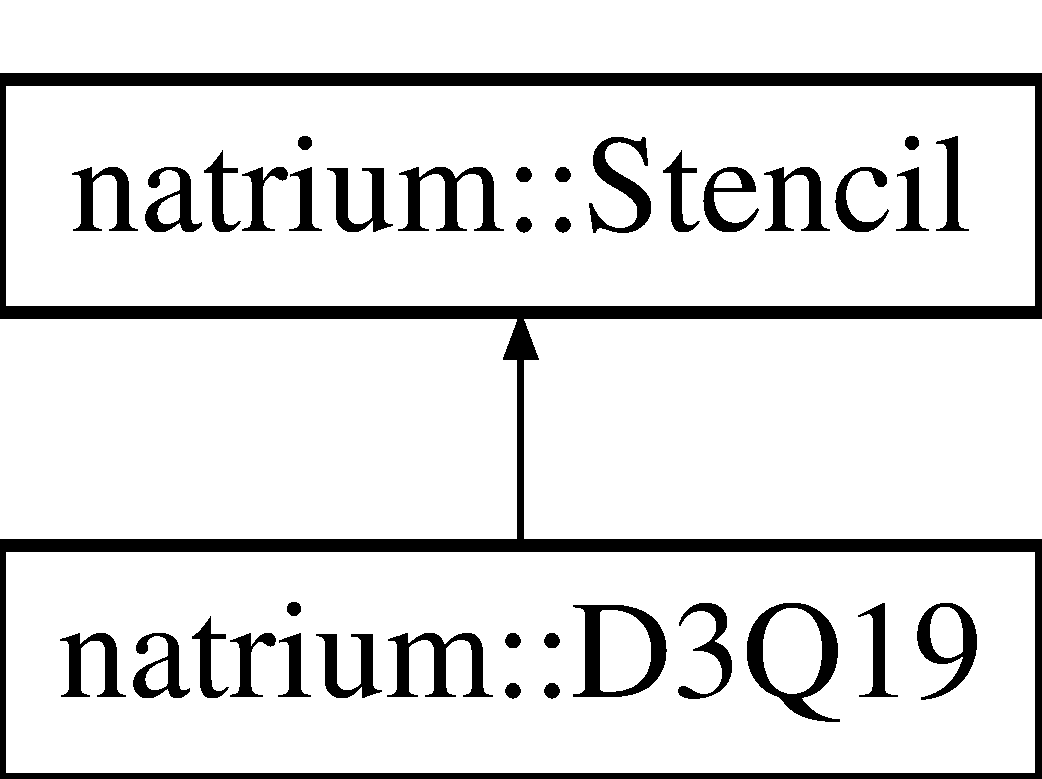
\includegraphics[height=2cm]{classnatrium_1_1D3Q19}
\end{center}
\end{figure}
\subsection*{Public Member Functions}
\begin{DoxyCompactItemize}
\item 
\hypertarget{classnatrium_1_1D3Q19_af5ebed1fc34e3496fdb02eedcb379357}{
\hyperlink{classnatrium_1_1D3Q19_af5ebed1fc34e3496fdb02eedcb379357}{D3Q19} (double scaling=1.0)}
\label{classnatrium_1_1D3Q19_af5ebed1fc34e3496fdb02eedcb379357}

\begin{DoxyCompactList}\small\item\em constructor \item\end{DoxyCompactList}\item 
\hypertarget{classnatrium_1_1D3Q19_a9ee5b7b88195b0757472b6179186474e}{
virtual \hyperlink{classnatrium_1_1D3Q19_a9ee5b7b88195b0757472b6179186474e}{$\sim$D3Q19} ()}
\label{classnatrium_1_1D3Q19_a9ee5b7b88195b0757472b6179186474e}

\begin{DoxyCompactList}\small\item\em destructor \item\end{DoxyCompactList}\item 
\hypertarget{classnatrium_1_1D3Q19_af2580d30fd2d3570db5bdf19b1f8bf44}{
virtual double {\bfseries getSpeedOfSound} () const }
\label{classnatrium_1_1D3Q19_af2580d30fd2d3570db5bdf19b1f8bf44}

\item 
\hypertarget{classnatrium_1_1D3Q19_aa57a051bfef2bd1253b59077f15daab7}{
virtual double {\bfseries getSpeedOfSoundSquare} () const }
\label{classnatrium_1_1D3Q19_aa57a051bfef2bd1253b59077f15daab7}

\item 
\hypertarget{classnatrium_1_1D3Q19_a0ba17a57d531a2ff80468d014a59b071}{
virtual size\_\-t {\bfseries getIndexOfOppositeDirection} (size\_\-t index) const }
\label{classnatrium_1_1D3Q19_a0ba17a57d531a2ff80468d014a59b071}

\item 
\hypertarget{classnatrium_1_1D3Q19_ace8b31d69b10b748f4951744425a8177}{
virtual double {\bfseries getMaxParticleVelocityMagnitude} () const }
\label{classnatrium_1_1D3Q19_ace8b31d69b10b748f4951744425a8177}

\item 
\hypertarget{classnatrium_1_1D3Q19_a5ae0a8c8d01e0613e22695d11446c64e}{
virtual double {\bfseries getScaling} () const }
\label{classnatrium_1_1D3Q19_a5ae0a8c8d01e0613e22695d11446c64e}

\end{DoxyCompactItemize}
\subsection*{Static Public Attributes}
\begin{DoxyCompactItemize}
\item 
\hypertarget{classnatrium_1_1D3Q19_a1eade3a56682d2e2f5533c811fc169fd}{
static const size\_\-t \hyperlink{classnatrium_1_1D3Q19_a1eade3a56682d2e2f5533c811fc169fd}{D} = 3}
\label{classnatrium_1_1D3Q19_a1eade3a56682d2e2f5533c811fc169fd}

\begin{DoxyCompactList}\small\item\em D. \item\end{DoxyCompactList}\item 
\hypertarget{classnatrium_1_1D3Q19_a8fa668ebc269adc347899954b189a2fb}{
static const size\_\-t \hyperlink{classnatrium_1_1D3Q19_a8fa668ebc269adc347899954b189a2fb}{Q} = 19}
\label{classnatrium_1_1D3Q19_a8fa668ebc269adc347899954b189a2fb}

\begin{DoxyCompactList}\small\item\em Q. \item\end{DoxyCompactList}\end{DoxyCompactItemize}
\subsection*{Protected Attributes}
\begin{DoxyCompactItemize}
\item 
\hypertarget{classnatrium_1_1D3Q19_aa993e9e0399c46c54a8d7abd9ba4ecb9}{
const double \hyperlink{classnatrium_1_1D3Q19_aa993e9e0399c46c54a8d7abd9ba4ecb9}{m\_\-speedOfSound}}
\label{classnatrium_1_1D3Q19_aa993e9e0399c46c54a8d7abd9ba4ecb9}

\begin{DoxyCompactList}\small\item\em speed of sound \item\end{DoxyCompactList}\item 
\hypertarget{classnatrium_1_1D3Q19_aee2e25de1cdfa530b98df8e09884c47b}{
const double \hyperlink{classnatrium_1_1D3Q19_aee2e25de1cdfa530b98df8e09884c47b}{m\_\-speedOfSoundSquare}}
\label{classnatrium_1_1D3Q19_aee2e25de1cdfa530b98df8e09884c47b}

\begin{DoxyCompactList}\small\item\em (speed of sound)$^\wedge$2 \item\end{DoxyCompactList}\item 
\hypertarget{classnatrium_1_1D3Q19_abe8a49d87735513e5c18091e8596bc38}{
const double \hyperlink{classnatrium_1_1D3Q19_abe8a49d87735513e5c18091e8596bc38}{m\_\-scaling}}
\label{classnatrium_1_1D3Q19_abe8a49d87735513e5c18091e8596bc38}

\begin{DoxyCompactList}\small\item\em scaling of the stencil \item\end{DoxyCompactList}\end{DoxyCompactItemize}


\subsection{Detailed Description}
\hyperlink{classnatrium_1_1D3Q19}{D3Q19} Model. The lattice velocities are: 0. 0.0 0.0 0.0. 
\begin{DoxyEnumerate}
\item scaling , 0.0, 0.0
\item 0.0 , 0.0, scaling
\item -\/scaling, 0.0 , 0.0
\item 0.0, 0.0 , -\/scaling
\item 0.0, -\/scaling , 0.0
\item 0.0, scaling , 0.0
\item scaling, 0.0 , scaling
\item -\/scaling , 0.0 , scaling
\item -\/scaling , 0.0 , -\/scaling
\item scaling , 0.0 , -\/scaling
\item scaling, -\/scaling, 0.0
\item scaling, scaling , 0.0
\item -\/scaling, scaling , 0.0
\item -\/scaling, -\/scaling , 0.0
\item 0.0, -\/scaling , scaling
\item 0.0, scaling , scaling
\item 0.0, scaling , -\/scaling
\item 0.0, -\/scaling , -\/scaling
\end{DoxyEnumerate}

The weights are:
\begin{DoxyItemize}
\item 0) 1./3.
\item 1-\/6) 1./18.
\item 7-\/18) 1./36. 
\end{DoxyItemize}

The documentation for this class was generated from the following files:\begin{DoxyCompactItemize}
\item 
/mnt/fdrive/akraem3m/workspace/NATriuM/src/library/natrium/stencils/D3Q19.h\item 
/mnt/fdrive/akraem3m/workspace/NATriuM/src/library/natrium/stencils/D3Q19.cpp\end{DoxyCompactItemize}

\hypertarget{classnatrium_1_1D3Q27}{
\section{natrium::D3Q27 Class Reference}
\label{classnatrium_1_1D3Q27}\index{natrium::D3Q27@{natrium::D3Q27}}
}


\hyperlink{classnatrium_1_1D3Q27}{D3Q27} Model. The lattice velocities are: 0. 0.0 0.0 0.0.  


{\ttfamily \#include $<$D3Q27.h$>$}Inheritance diagram for natrium::D3Q27::\begin{figure}[H]
\begin{center}
\leavevmode
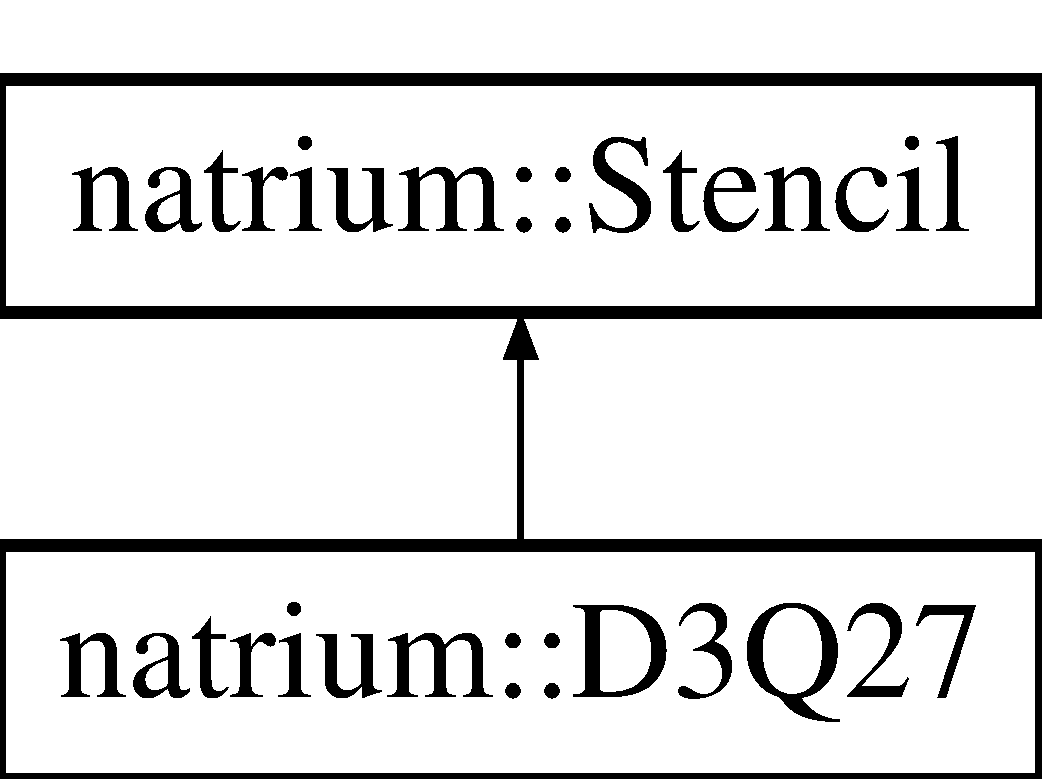
\includegraphics[height=2cm]{classnatrium_1_1D3Q27}
\end{center}
\end{figure}
\subsection*{Public Member Functions}
\begin{DoxyCompactItemize}
\item 
\hypertarget{classnatrium_1_1D3Q27_abd86172df2f60b7631d3732b86a8bad6}{
\hyperlink{classnatrium_1_1D3Q27_abd86172df2f60b7631d3732b86a8bad6}{D3Q27} (double scaling=1.0)}
\label{classnatrium_1_1D3Q27_abd86172df2f60b7631d3732b86a8bad6}

\begin{DoxyCompactList}\small\item\em constructor \item\end{DoxyCompactList}\item 
\hypertarget{classnatrium_1_1D3Q27_a0472abd51ed764619f3f761037f92e08}{
virtual \hyperlink{classnatrium_1_1D3Q27_a0472abd51ed764619f3f761037f92e08}{$\sim$D3Q27} ()}
\label{classnatrium_1_1D3Q27_a0472abd51ed764619f3f761037f92e08}

\begin{DoxyCompactList}\small\item\em destructor \item\end{DoxyCompactList}\item 
\hypertarget{classnatrium_1_1D3Q27_a66878d6b823046345df5374badbe499f}{
virtual double {\bfseries getSpeedOfSound} () const }
\label{classnatrium_1_1D3Q27_a66878d6b823046345df5374badbe499f}

\item 
\hypertarget{classnatrium_1_1D3Q27_ad810fc7813c4433638a146149b674b63}{
virtual double {\bfseries getSpeedOfSoundSquare} () const }
\label{classnatrium_1_1D3Q27_ad810fc7813c4433638a146149b674b63}

\item 
\hypertarget{classnatrium_1_1D3Q27_a28aadecf909da8bcba7ec0ba65628cc0}{
virtual size\_\-t {\bfseries getIndexOfOppositeDirection} (size\_\-t index) const }
\label{classnatrium_1_1D3Q27_a28aadecf909da8bcba7ec0ba65628cc0}

\item 
\hypertarget{classnatrium_1_1D3Q27_a1dbd203cc4524d40f37fab9b2bb27471}{
virtual double {\bfseries getMaxParticleVelocityMagnitude} () const }
\label{classnatrium_1_1D3Q27_a1dbd203cc4524d40f37fab9b2bb27471}

\item 
\hypertarget{classnatrium_1_1D3Q27_a04500e67bdea5a8f9e39bc8631d1d1f4}{
virtual double {\bfseries getScaling} () const }
\label{classnatrium_1_1D3Q27_a04500e67bdea5a8f9e39bc8631d1d1f4}

\end{DoxyCompactItemize}
\subsection*{Static Public Attributes}
\begin{DoxyCompactItemize}
\item 
\hypertarget{classnatrium_1_1D3Q27_a70ac295cb0d619520d3f9d1cc062a8f9}{
static const size\_\-t \hyperlink{classnatrium_1_1D3Q27_a70ac295cb0d619520d3f9d1cc062a8f9}{D} = 3}
\label{classnatrium_1_1D3Q27_a70ac295cb0d619520d3f9d1cc062a8f9}

\begin{DoxyCompactList}\small\item\em D. \item\end{DoxyCompactList}\item 
\hypertarget{classnatrium_1_1D3Q27_ad15f9c712c68bd3457bdf3560fd25226}{
static const size\_\-t \hyperlink{classnatrium_1_1D3Q27_ad15f9c712c68bd3457bdf3560fd25226}{Q} = 27}
\label{classnatrium_1_1D3Q27_ad15f9c712c68bd3457bdf3560fd25226}

\begin{DoxyCompactList}\small\item\em Q. \item\end{DoxyCompactList}\end{DoxyCompactItemize}
\subsection*{Protected Member Functions}
\begin{DoxyCompactItemize}
\item 
\hypertarget{classnatrium_1_1D3Q27_af8fb063c24736837bf33c19d2a376ca8}{
\hyperlink{namespacenatrium_ad8cbec7aab93a74837b06ded39615d47}{numeric\_\-matrix} \hyperlink{classnatrium_1_1D3Q27_af8fb063c24736837bf33c19d2a376ca8}{makeMomentBasis} (vector$<$ \hyperlink{namespacenatrium_a67c39077adc6634f8fa3762b8eef24c4}{numeric\_\-vector} $>$ e)}
\label{classnatrium_1_1D3Q27_af8fb063c24736837bf33c19d2a376ca8}

\begin{DoxyCompactList}\small\item\em make directions \item\end{DoxyCompactList}\end{DoxyCompactItemize}
\subsection*{Protected Attributes}
\begin{DoxyCompactItemize}
\item 
\hypertarget{classnatrium_1_1D3Q27_aa51ddf8624a7a077e2363c5a746ad5ec}{
const double \hyperlink{classnatrium_1_1D3Q27_aa51ddf8624a7a077e2363c5a746ad5ec}{m\_\-speedOfSound}}
\label{classnatrium_1_1D3Q27_aa51ddf8624a7a077e2363c5a746ad5ec}

\begin{DoxyCompactList}\small\item\em speed of sound \item\end{DoxyCompactList}\item 
\hypertarget{classnatrium_1_1D3Q27_a0a085448ff47a3586e1f9cd593c6bfa4}{
const double \hyperlink{classnatrium_1_1D3Q27_a0a085448ff47a3586e1f9cd593c6bfa4}{m\_\-speedOfSoundSquare}}
\label{classnatrium_1_1D3Q27_a0a085448ff47a3586e1f9cd593c6bfa4}

\begin{DoxyCompactList}\small\item\em (speed of sound)$^\wedge$2 \item\end{DoxyCompactList}\item 
\hypertarget{classnatrium_1_1D3Q27_a1e13c07988d781168d794c89ee3c6977}{
const double \hyperlink{classnatrium_1_1D3Q27_a1e13c07988d781168d794c89ee3c6977}{m\_\-scaling}}
\label{classnatrium_1_1D3Q27_a1e13c07988d781168d794c89ee3c6977}

\begin{DoxyCompactList}\small\item\em scaling of the stencil \item\end{DoxyCompactList}\end{DoxyCompactItemize}


\subsection{Detailed Description}
\hyperlink{classnatrium_1_1D3Q27}{D3Q27} Model. The lattice velocities are: 0. 0.0 0.0 0.0. 
\begin{DoxyEnumerate}
\item scaling, 0.0, 0.0
\item -\/scaling, 0.0, 0.0
\item 0.0, scaling, 0.0
\item 0.0, -\/scaling, 0.0
\item 0.0, 0.0, scaling
\item 0.0, 0.0, -\/scaling
\item 0.0, scaling, scaling
\item 0.0, -\/scaling -\/ scaling
\item 0.0, scaling, -\/scaling
\item 0.0, -\/scaling, scaling
\item scaling, 0.0, scaling
\item -\/scaling, 0.0, -\/scaling
\item scaling, 0.0, -\/scaling
\item -\/scaling, 0.0, scaling
\item scaling, scaling, 0.0
\item -\/scaling, -\/scaling, 0.0
\item scaling, -\/scaling, 0.0
\item -\/scaling, scaling, 0.0
\item scaling, scaling, scaling
\item -\/scaling, -\/scaling, -\/scaling
\item scaling, scaling, -\/scaling
\item -\/scaling, -\/scaling, scaling
\item scaling, -\/scaling, scaling
\item -\/scaling, scaling, -\/scaling
\item scaling, -\/scaling, -\/scaling
\item -\/scaling, scaling, scaling
\end{DoxyEnumerate}

The weights are:
\begin{DoxyItemize}
\item 0) 8./27.
\item 1-\/6) 2./27.
\item 7-\/18) 1./54.
\item 19-\/26) 1./216. 
\end{DoxyItemize}

The documentation for this class was generated from the following files:\begin{DoxyCompactItemize}
\item 
/mnt/fdrive/akraem3m/workspace/NATriuM/src/library/natrium/stencils/D3Q27.h\item 
/mnt/fdrive/akraem3m/workspace/NATriuM/src/library/natrium/stencils/D3Q27.cpp\end{DoxyCompactItemize}

\hypertarget{classnatrium_1_1DataProcessor}{
\section{natrium::DataProcessor$<$ dim $>$ Class Template Reference}
\label{classnatrium_1_1DataProcessor}\index{natrium::DataProcessor@{natrium::DataProcessor}}
}
Inheritance diagram for natrium::DataProcessor$<$ dim $>$::\begin{figure}[H]
\begin{center}
\leavevmode
\includegraphics[height=2cm]{classnatrium_1_1DataProcessor}
\end{center}
\end{figure}
\subsection*{Public Member Functions}
\begin{DoxyCompactItemize}
\item 
\hypertarget{classnatrium_1_1DataProcessor_a22a635f9a3336b375e8e8345a82f592d}{
{\bfseries DataProcessor} (\hyperlink{classnatrium_1_1CFDSolver}{CFDSolver}$<$ dim $>$ \&solver)}
\label{classnatrium_1_1DataProcessor_a22a635f9a3336b375e8e8345a82f592d}

\item 
\hypertarget{classnatrium_1_1DataProcessor_a82939cd7d981e39d2f4f2483b79e03dd}{
virtual void {\bfseries apply} ()=0}
\label{classnatrium_1_1DataProcessor_a82939cd7d981e39d2f4f2483b79e03dd}

\end{DoxyCompactItemize}
\subsection*{Protected Attributes}
\begin{DoxyCompactItemize}
\item 
\hypertarget{classnatrium_1_1DataProcessor_ae0be34660f37d5ae8bad42b46383d7fe}{
\hyperlink{classnatrium_1_1CFDSolver}{CFDSolver}$<$ dim $>$ \& {\bfseries m\_\-solver}}
\label{classnatrium_1_1DataProcessor_ae0be34660f37d5ae8bad42b46383d7fe}

\end{DoxyCompactItemize}
\subsubsection*{template$<$size\_\-t dim$>$ class natrium::DataProcessor$<$ dim $>$}



The documentation for this class was generated from the following file:\begin{DoxyCompactItemize}
\item 
/mnt/fdrive/akraem3m/workspace/NATriuM/src/library/natrium/dataprocessors/DataProcessor.h\end{DoxyCompactItemize}

\hypertarget{classnatrium_1_1DealIIWrapper}{\section{natrium\-:\-:Deal\-I\-I\-Wrapper$<$ M\-A\-T\-R\-I\-X, V\-E\-C\-T\-O\-R $>$ Class Template Reference}
\label{classnatrium_1_1DealIIWrapper}\index{natrium\-::\-Deal\-I\-I\-Wrapper$<$ M\-A\-T\-R\-I\-X, V\-E\-C\-T\-O\-R $>$@{natrium\-::\-Deal\-I\-I\-Wrapper$<$ M\-A\-T\-R\-I\-X, V\-E\-C\-T\-O\-R $>$}}
}


not yet implemented  




{\ttfamily \#include $<$Deal\-I\-I\-Wrapper.\-h$>$}

\subsection*{Public Member Functions}
\begin{DoxyCompactItemize}
\item 
\hypertarget{classnatrium_1_1DealIIWrapper_a879ff25fa485bdffecbdf6083d0c3d45}{virtual void {\bfseries step} (V\-E\-C\-T\-O\-R \&vector, const M\-A\-T\-R\-I\-X \&system\-Matrix, const V\-E\-C\-T\-O\-R \&system\-Vector)}\label{classnatrium_1_1DealIIWrapper_a879ff25fa485bdffecbdf6083d0c3d45}

\end{DoxyCompactItemize}


\subsection{Detailed Description}
\subsubsection*{template$<$class M\-A\-T\-R\-I\-X, class V\-E\-C\-T\-O\-R$>$class natrium\-::\-Deal\-I\-I\-Wrapper$<$ M\-A\-T\-R\-I\-X, V\-E\-C\-T\-O\-R $>$}

not yet implemented 

The documentation for this class was generated from the following files\-:\begin{DoxyCompactItemize}
\item 
/home/kraemer/eclipse\-\_\-workspace/\-N\-A\-Triu\-M/src/natrium/timeintegration/Deal\-I\-I\-Wrapper.\-h\item 
/home/kraemer/eclipse\-\_\-workspace/\-N\-A\-Triu\-M/src/natrium/timeintegration/Deal\-I\-I\-Wrapper.\-cpp\end{DoxyCompactItemize}

\hypertarget{classnatrium_1_1DecayingTurbulence2D}{
\section{natrium::DecayingTurbulence2D Class Reference}
\label{classnatrium_1_1DecayingTurbulence2D}\index{natrium::DecayingTurbulence2D@{natrium::DecayingTurbulence2D}}
}


Description of a turbulent Channel Flow The domain is \mbox{[}0,5\mbox{]}x\mbox{[}0,1\mbox{]}.  


{\ttfamily \#include $<$DecayingTurbulence2D.h$>$}Inheritance diagram for natrium::DecayingTurbulence2D::\begin{figure}[H]
\begin{center}
\leavevmode
\includegraphics[height=2cm]{classnatrium_1_1DecayingTurbulence2D}
\end{center}
\end{figure}
\subsection*{Classes}
\begin{DoxyCompactItemize}
\item 
class \hyperlink{classnatrium_1_1DecayingTurbulence2D_1_1InitialVelocity}{InitialVelocity}
\begin{DoxyCompactList}\small\item\em class to describe the x-\/component of the analytic solution \item\end{DoxyCompactList}\end{DoxyCompactItemize}
\subsection*{Public Member Functions}
\begin{DoxyCompactItemize}
\item 
\hyperlink{classnatrium_1_1DecayingTurbulence2D_af1aebee0f89465ec385a1a749f0ceb76}{DecayingTurbulence2D} (double viscosity, size\_\-t refinementLevel)
\begin{DoxyCompactList}\small\item\em constructor \item\end{DoxyCompactList}\item 
\hypertarget{classnatrium_1_1DecayingTurbulence2D_a82284a66335b86b3d82c2dca05ab6a77}{
virtual \hyperlink{classnatrium_1_1DecayingTurbulence2D_a82284a66335b86b3d82c2dca05ab6a77}{$\sim$DecayingTurbulence2D} ()}
\label{classnatrium_1_1DecayingTurbulence2D_a82284a66335b86b3d82c2dca05ab6a77}

\begin{DoxyCompactList}\small\item\em destructor \item\end{DoxyCompactList}\item 
\hypertarget{classnatrium_1_1DecayingTurbulence2D_a55dba4c6ae8523bc144db1bfe3a72951}{
virtual double {\bfseries getCharacteristicVelocity} () const }
\label{classnatrium_1_1DecayingTurbulence2D_a55dba4c6ae8523bc144db1bfe3a72951}

\item 
\hypertarget{classnatrium_1_1DecayingTurbulence2D_a391fe8a9c2ccaf4aaf6fcde4ea9e88f0}{
virtual void {\bfseries refine} (Mesh$<$ 2 $>$ \&mesh)}
\label{classnatrium_1_1DecayingTurbulence2D_a391fe8a9c2ccaf4aaf6fcde4ea9e88f0}

\item 
\hypertarget{classnatrium_1_1DecayingTurbulence2D_a1d5c4e7c4addab6647514ed4e102c181}{
virtual void {\bfseries transform} (Mesh$<$ 2 $>$ \&mesh)}
\label{classnatrium_1_1DecayingTurbulence2D_a1d5c4e7c4addab6647514ed4e102c181}

\item 
\hypertarget{classnatrium_1_1DecayingTurbulence2D_aa61a142ac3553e004dc053094819d816}{
virtual bool {\bfseries isCartesian} ()}
\label{classnatrium_1_1DecayingTurbulence2D_aa61a142ac3553e004dc053094819d816}

\end{DoxyCompactItemize}


\subsection{Detailed Description}
Description of a turbulent Channel Flow The domain is \mbox{[}0,5\mbox{]}x\mbox{[}0,1\mbox{]}. 

\subsection{Constructor \& Destructor Documentation}
\hypertarget{classnatrium_1_1DecayingTurbulence2D_af1aebee0f89465ec385a1a749f0ceb76}{
\index{natrium::DecayingTurbulence2D@{natrium::DecayingTurbulence2D}!DecayingTurbulence2D@{DecayingTurbulence2D}}
\index{DecayingTurbulence2D@{DecayingTurbulence2D}!natrium::DecayingTurbulence2D@{natrium::DecayingTurbulence2D}}
\subsubsection[{DecayingTurbulence2D}]{\setlength{\rightskip}{0pt plus 5cm}natrium::DecayingTurbulence2D::DecayingTurbulence2D (double {\em viscosity}, \/  size\_\-t {\em refinementLevel})}}
\label{classnatrium_1_1DecayingTurbulence2D_af1aebee0f89465ec385a1a749f0ceb76}


constructor 

apply boundary values 

The documentation for this class was generated from the following files:\begin{DoxyCompactItemize}
\item 
/mnt/fdrive/akraem3m/workspace/NATriuM/src/examples/step-\/decayingTurbulence2D/\hyperlink{DecayingTurbulence2D_8h}{DecayingTurbulence2D.h}\item 
/mnt/fdrive/akraem3m/workspace/NATriuM/src/examples/step-\/decayingTurbulence2D/DecayingTurbulence2D.cpp\end{DoxyCompactItemize}

\hypertarget{classnatrium_1_1DensityFluctuation2D}{\section{natrium\-:\-:Density\-Fluctuation2\-D Class Reference}
\label{classnatrium_1_1DensityFluctuation2D}\index{natrium\-::\-Density\-Fluctuation2\-D@{natrium\-::\-Density\-Fluctuation2\-D}}
}
Inheritance diagram for natrium\-:\-:Density\-Fluctuation2\-D\-:\begin{figure}[H]
\begin{center}
\leavevmode
\includegraphics[height=2.000000cm]{classnatrium_1_1DensityFluctuation2D}
\end{center}
\end{figure}
\subsection*{Public Member Functions}
\begin{DoxyCompactItemize}
\item 
\hypertarget{classnatrium_1_1DensityFluctuation2D_aac8ea303ea740e73868cd1ee431e182f}{{\bfseries Density\-Fluctuation2\-D} (double viscosity, size\-\_\-t refinement\-Level)}\label{classnatrium_1_1DensityFluctuation2D_aac8ea303ea740e73868cd1ee431e182f}

\item 
\hypertarget{classnatrium_1_1DensityFluctuation2D_a7d345499b56b65e0b107defcd5c89e2e}{virtual void {\bfseries apply\-Initial\-Densities} (distributed\-\_\-vector \&initial\-Densities, const vector$<$ dealii\-::\-Point$<$ 2 $>$ $>$ \&support\-Points) const }\label{classnatrium_1_1DensityFluctuation2D_a7d345499b56b65e0b107defcd5c89e2e}

\item 
\hypertarget{classnatrium_1_1DensityFluctuation2D_a217a8d3635da81fb0350671a86142b57}{virtual void {\bfseries apply\-Initial\-Velocities} (vector$<$ distributed\-\_\-vector $>$ \&initial\-Velocities, const vector$<$ dealii\-::\-Point$<$ 2 $>$ $>$ \&support\-Points) const }\label{classnatrium_1_1DensityFluctuation2D_a217a8d3635da81fb0350671a86142b57}

\end{DoxyCompactItemize}


The documentation for this class was generated from the following files\-:\begin{DoxyCompactItemize}
\item 
/home/kraemer/eclipse\-\_\-workspace/\-N\-A\-Triu\-M/src/examples/step-\/99/Density\-Fluctuation2\-D.\-h\item 
/home/kraemer/eclipse\-\_\-workspace/\-N\-A\-Triu\-M/src/examples/step-\/99/Density\-Fluctuation2\-D.\-cpp\end{DoxyCompactItemize}

\hypertarget{classnatrium_1_1DiamondObstacle2D}{
\section{natrium::DiamondObstacle2D Class Reference}
\label{classnatrium_1_1DiamondObstacle2D}\index{natrium::DiamondObstacle2D@{natrium::DiamondObstacle2D}}
}


Description of a flow around a diamond-\/shaped obstacle.  


{\ttfamily \#include $<$DiamondObstacle2D.h$>$}Inheritance diagram for natrium::DiamondObstacle2D::\begin{figure}[H]
\begin{center}
\leavevmode
\includegraphics[height=2cm]{classnatrium_1_1DiamondObstacle2D}
\end{center}
\end{figure}
\subsection*{Classes}
\begin{DoxyCompactItemize}
\item 
class \hyperlink{classnatrium_1_1DiamondObstacle2D_1_1InflowVelocity}{InflowVelocity}
\end{DoxyCompactItemize}
\subsection*{Public Member Functions}
\begin{DoxyCompactItemize}
\item 
\hyperlink{classnatrium_1_1DiamondObstacle2D_a466c22e26de373b06ccba9c5e0a23c33}{DiamondObstacle2D} (double velocity, double viscosity, size\_\-t refinementLevel)
\begin{DoxyCompactList}\small\item\em constructor \item\end{DoxyCompactList}\item 
\hypertarget{classnatrium_1_1DiamondObstacle2D_a96119fe50e043dae093912884798d9a5}{
virtual \hyperlink{classnatrium_1_1DiamondObstacle2D_a96119fe50e043dae093912884798d9a5}{$\sim$DiamondObstacle2D} ()}
\label{classnatrium_1_1DiamondObstacle2D_a96119fe50e043dae093912884798d9a5}

\begin{DoxyCompactList}\small\item\em destructor \item\end{DoxyCompactList}\item 
\hypertarget{classnatrium_1_1DiamondObstacle2D_a9edc6d74879f7edd811b7180c1156a04}{
virtual double {\bfseries getCharacteristicVelocity} () const }
\label{classnatrium_1_1DiamondObstacle2D_a9edc6d74879f7edd811b7180c1156a04}

\item 
\hypertarget{classnatrium_1_1DiamondObstacle2D_a6fd173230aeb5e15db27d7f2a752df5a}{
virtual void {\bfseries refine} (Mesh$<$ 2 $>$ \&mesh)}
\label{classnatrium_1_1DiamondObstacle2D_a6fd173230aeb5e15db27d7f2a752df5a}

\item 
\hypertarget{classnatrium_1_1DiamondObstacle2D_a6a51680cf76b665f5eaedcf7d66acfec}{
virtual void {\bfseries transform} (Mesh$<$ 2 $>$ \&)}
\label{classnatrium_1_1DiamondObstacle2D_a6a51680cf76b665f5eaedcf7d66acfec}

\item 
\hypertarget{classnatrium_1_1DiamondObstacle2D_a323f8c082fd7b49547c72f1c416665f7}{
virtual bool {\bfseries isCartesian} ()}
\label{classnatrium_1_1DiamondObstacle2D_a323f8c082fd7b49547c72f1c416665f7}

\end{DoxyCompactItemize}


\subsection{Detailed Description}
Description of a flow around a diamond-\/shaped obstacle. 

\subsection{Constructor \& Destructor Documentation}
\hypertarget{classnatrium_1_1DiamondObstacle2D_a466c22e26de373b06ccba9c5e0a23c33}{
\index{natrium::DiamondObstacle2D@{natrium::DiamondObstacle2D}!DiamondObstacle2D@{DiamondObstacle2D}}
\index{DiamondObstacle2D@{DiamondObstacle2D}!natrium::DiamondObstacle2D@{natrium::DiamondObstacle2D}}
\subsubsection[{DiamondObstacle2D}]{\setlength{\rightskip}{0pt plus 5cm}natrium::DiamondObstacle2D::DiamondObstacle2D (double {\em velocity}, \/  double {\em viscosity}, \/  size\_\-t {\em refinementLevel})}}
\label{classnatrium_1_1DiamondObstacle2D_a466c22e26de373b06ccba9c5e0a23c33}


constructor 

apply boundary values 

The documentation for this class was generated from the following files:\begin{DoxyCompactItemize}
\item 
/mnt/fdrive/akraem3m/workspace/NATriuM/src/examples/step-\/grid-\/in/\hyperlink{DiamondObstacle2D_8h}{DiamondObstacle2D.h}\item 
/mnt/fdrive/akraem3m/workspace/NATriuM/src/examples/step-\/grid-\/in/\hyperlink{DiamondObstacle2D_8cpp}{DiamondObstacle2D.cpp}\end{DoxyCompactItemize}

\hypertarget{classDiffFunction2D}{
\section{DiffFunction2D Class Reference}
\label{classDiffFunction2D}\index{DiffFunction2D@{DiffFunction2D}}
}
\subsection*{Public Member Functions}
\begin{DoxyCompactItemize}
\item 
\hypertarget{classDiffFunction2D_af8fa31d8793f813b678ee683bdabe4c7}{
virtual double {\bfseries value} (const dealii::Point$<$ 2 $>$ \&points, const unsigned int component) const }
\label{classDiffFunction2D_af8fa31d8793f813b678ee683bdabe4c7}

\end{DoxyCompactItemize}


The documentation for this class was generated from the following file:\begin{DoxyCompactItemize}
\item 
/mnt/fdrive/akraem3m/workspace/NATriuM/src/test/utilities/ContinuousGradient\_\-test.cpp\end{DoxyCompactItemize}

\hypertarget{classDiffFunction3D}{
\section{DiffFunction3D Class Reference}
\label{classDiffFunction3D}\index{DiffFunction3D@{DiffFunction3D}}
}
\subsection*{Public Member Functions}
\begin{DoxyCompactItemize}
\item 
\hypertarget{classDiffFunction3D_a7fb1fe9820e72a600f0a19859a45c7c5}{
virtual double {\bfseries value} (const dealii::Point$<$ 3 $>$ \&points, const unsigned int component) const }
\label{classDiffFunction3D_a7fb1fe9820e72a600f0a19859a45c7c5}

\end{DoxyCompactItemize}


The documentation for this class was generated from the following file:\begin{DoxyCompactItemize}
\item 
/mnt/fdrive/akraem3m/workspace/NATriuM/src/test/utilities/ContinuousGradient\_\-test.cpp\end{DoxyCompactItemize}

\hypertarget{classnatrium_1_1DistributionFunctions}{
\section{natrium::DistributionFunctions Class Reference}
\label{classnatrium_1_1DistributionFunctions}\index{natrium::DistributionFunctions@{natrium::DistributionFunctions}}
}


This class contains the distribution functions. As the zero-\/velocity particles (f0) can be ignored for streaming, f0 is split from the other distribution functions (fStream) in the implementation. fStream is a block vector, which has the advantage that it can be multiplied with the SystemMatrix. The \hyperlink{classnatrium_1_1DistributionFunctions}{DistributionFunctions} class is designed to mime the behaviour of a vector$<$distributed\_\-vector$>$ .  


{\ttfamily \#include $<$DistributionFunctions.h$>$}\subsection*{Public Member Functions}
\begin{DoxyCompactItemize}
\item 
\hyperlink{classnatrium_1_1DistributionFunctions_a3c886085011c99c505cdfc4903e20dfd}{DistributionFunctions} (bool dg=true)
\begin{DoxyCompactList}\small\item\em empty constructor. Construction is done through reinit. \item\end{DoxyCompactList}\item 
\hypertarget{classnatrium_1_1DistributionFunctions_af0a970355419acf79be898e573f3149a}{
\hyperlink{classnatrium_1_1DistributionFunctions_af0a970355419acf79be898e573f3149a}{DistributionFunctions} (const \hyperlink{classnatrium_1_1DistributionFunctions}{DistributionFunctions} \&f)}
\label{classnatrium_1_1DistributionFunctions_af0a970355419acf79be898e573f3149a}

\begin{DoxyCompactList}\small\item\em Copy constructor. \item\end{DoxyCompactList}\item 
\hypertarget{classnatrium_1_1DistributionFunctions_a43739b1d781e72fa21740dc4dcfe7a54}{
\hyperlink{classnatrium_1_1DistributionFunctions_a43739b1d781e72fa21740dc4dcfe7a54}{DistributionFunctions} (const vector$<$ \hyperlink{namespacenatrium_a903d2b92917f582f2ff05f52160ab811}{distributed\_\-vector} $>$ \&f, bool dg=true)}
\label{classnatrium_1_1DistributionFunctions_a43739b1d781e72fa21740dc4dcfe7a54}

\begin{DoxyCompactList}\small\item\em Copy constructor. Conversion from vector$<$distributed\_\-vector$>$. \item\end{DoxyCompactList}\item 
\hypertarget{classnatrium_1_1DistributionFunctions_af965a46fbf124e8f90250c843e615bcd}{
virtual \hyperlink{classnatrium_1_1DistributionFunctions_af965a46fbf124e8f90250c843e615bcd}{$\sim$DistributionFunctions} ()}
\label{classnatrium_1_1DistributionFunctions_af965a46fbf124e8f90250c843e615bcd}

\begin{DoxyCompactList}\small\item\em Destructor. \item\end{DoxyCompactList}\item 
\hypertarget{classnatrium_1_1DistributionFunctions_af8b473d257152e9d588030eac9500d08}{
\hyperlink{namespacenatrium_a903d2b92917f582f2ff05f52160ab811}{distributed\_\-vector} \& \hyperlink{classnatrium_1_1DistributionFunctions_af8b473d257152e9d588030eac9500d08}{at} (size\_\-t i)}
\label{classnatrium_1_1DistributionFunctions_af8b473d257152e9d588030eac9500d08}

\begin{DoxyCompactList}\small\item\em mimes std::vector.at(i) \item\end{DoxyCompactList}\item 
\hypertarget{classnatrium_1_1DistributionFunctions_a55af3d8382ed4c46d88e86a8f41844f7}{
const \hyperlink{namespacenatrium_a903d2b92917f582f2ff05f52160ab811}{distributed\_\-vector} \& \hyperlink{classnatrium_1_1DistributionFunctions_a55af3d8382ed4c46d88e86a8f41844f7}{at} (size\_\-t i) const }
\label{classnatrium_1_1DistributionFunctions_a55af3d8382ed4c46d88e86a8f41844f7}

\begin{DoxyCompactList}\small\item\em mimes std::vector.at(i) \item\end{DoxyCompactList}\item 
\hypertarget{classnatrium_1_1DistributionFunctions_a1a3dd164bf6f2519b142c7eaa950daa6}{
\hyperlink{namespacenatrium_a903d2b92917f582f2ff05f52160ab811}{distributed\_\-vector} \& \hyperlink{classnatrium_1_1DistributionFunctions_a1a3dd164bf6f2519b142c7eaa950daa6}{atGhosted} (size\_\-t i)}
\label{classnatrium_1_1DistributionFunctions_a1a3dd164bf6f2519b142c7eaa950daa6}

\begin{DoxyCompactList}\small\item\em mimes std::vector.at(i) \item\end{DoxyCompactList}\item 
\hypertarget{classnatrium_1_1DistributionFunctions_a10d928c2587e6a747ca330f57e72e819}{
const \hyperlink{namespacenatrium_a903d2b92917f582f2ff05f52160ab811}{distributed\_\-vector} \& \hyperlink{classnatrium_1_1DistributionFunctions_a10d928c2587e6a747ca330f57e72e819}{atGhosted} (size\_\-t i) const }
\label{classnatrium_1_1DistributionFunctions_a10d928c2587e6a747ca330f57e72e819}

\begin{DoxyCompactList}\small\item\em mimes std::vector.at(i) \item\end{DoxyCompactList}\item 
\hypertarget{classnatrium_1_1DistributionFunctions_a3d76ae4f928f324ec82099dbdce678d7}{
const \hyperlink{namespacenatrium_a903d2b92917f582f2ff05f52160ab811}{distributed\_\-vector} \& \hyperlink{classnatrium_1_1DistributionFunctions_a3d76ae4f928f324ec82099dbdce678d7}{getF0} () const }
\label{classnatrium_1_1DistributionFunctions_a3d76ae4f928f324ec82099dbdce678d7}

\begin{DoxyCompactList}\small\item\em F0 denotes the vector $ f_0 $ (zero-\/velocity particles). \item\end{DoxyCompactList}\item 
\hypertarget{classnatrium_1_1DistributionFunctions_abb98df52461532f58e77741dd9b6a975}{
\hyperlink{namespacenatrium_a903d2b92917f582f2ff05f52160ab811}{distributed\_\-vector} \& \hyperlink{classnatrium_1_1DistributionFunctions_abb98df52461532f58e77741dd9b6a975}{getF0} ()}
\label{classnatrium_1_1DistributionFunctions_abb98df52461532f58e77741dd9b6a975}

\begin{DoxyCompactList}\small\item\em F0 denotes the vector $ f_0 $ (zero-\/velocity particles). \item\end{DoxyCompactList}\item 
\hypertarget{classnatrium_1_1DistributionFunctions_ae7cc68f9576384b3fbec8f171856f607}{
void \hyperlink{classnatrium_1_1DistributionFunctions_ae7cc68f9576384b3fbec8f171856f607}{setF0} (const \hyperlink{namespacenatrium_a903d2b92917f582f2ff05f52160ab811}{distributed\_\-vector} \&f0)}
\label{classnatrium_1_1DistributionFunctions_ae7cc68f9576384b3fbec8f171856f607}

\begin{DoxyCompactList}\small\item\em F0 denotes the vector $ f_0 $ (zero-\/velocity particles). \item\end{DoxyCompactList}\item 
\hypertarget{classnatrium_1_1DistributionFunctions_a74dfe8e6ac6d5f463dcb8220f37800a3}{
distributed\_\-block\_\-vector \& \hyperlink{classnatrium_1_1DistributionFunctions_a74dfe8e6ac6d5f463dcb8220f37800a3}{getFStream} ()}
\label{classnatrium_1_1DistributionFunctions_a74dfe8e6ac6d5f463dcb8220f37800a3}

\begin{DoxyCompactList}\small\item\em FStream denotes the block vector containing the vectors $ f_1, ..., f_Q $. \item\end{DoxyCompactList}\item 
\hypertarget{classnatrium_1_1DistributionFunctions_a88224d528262c522ea2ad8bec11178c1}{
const distributed\_\-block\_\-vector \& \hyperlink{classnatrium_1_1DistributionFunctions_a88224d528262c522ea2ad8bec11178c1}{getFStream} () const }
\label{classnatrium_1_1DistributionFunctions_a88224d528262c522ea2ad8bec11178c1}

\begin{DoxyCompactList}\small\item\em FStream denotes the block vector containing the vectors $ f_1, ..., f_Q $. \item\end{DoxyCompactList}\item 
\hypertarget{classnatrium_1_1DistributionFunctions_a79d29cb24887e83728fb2f94b611ecb8}{
const \hyperlink{namespacenatrium_a903d2b92917f582f2ff05f52160ab811}{distributed\_\-vector} \& \hyperlink{classnatrium_1_1DistributionFunctions_a79d29cb24887e83728fb2f94b611ecb8}{getF0Ghosted} ()}
\label{classnatrium_1_1DistributionFunctions_a79d29cb24887e83728fb2f94b611ecb8}

\begin{DoxyCompactList}\small\item\em F0 denotes the vector $ f_0 $ (zero-\/velocity particles). \item\end{DoxyCompactList}\item 
const distributed\_\-block\_\-vector \& \hyperlink{classnatrium_1_1DistributionFunctions_acc97fc1ac5185c94d8d15024c168b6c2}{getFStreamGhosted} () const 
\begin{DoxyCompactList}\small\item\em F0 denotes the vector $ f_0 $ (zero-\/velocity particles). \item\end{DoxyCompactList}\item 
\hypertarget{classnatrium_1_1DistributionFunctions_ad0ada0c54968a61f78eb1b82eb6c5a68}{
void \hyperlink{classnatrium_1_1DistributionFunctions_ad0ada0c54968a61f78eb1b82eb6c5a68}{setFStream} (const distributed\_\-block\_\-vector \&fStream)}
\label{classnatrium_1_1DistributionFunctions_ad0ada0c54968a61f78eb1b82eb6c5a68}

\begin{DoxyCompactList}\small\item\em FStream denotes the block vector containing the vectors $ f_1, ..., f_Q $. \item\end{DoxyCompactList}\item 
\hypertarget{classnatrium_1_1DistributionFunctions_a2ab8e5abf8cdef76f62e443a8dde5fd4}{
size\_\-t \hyperlink{classnatrium_1_1DistributionFunctions_a2ab8e5abf8cdef76f62e443a8dde5fd4}{getQ} () const }
\label{classnatrium_1_1DistributionFunctions_a2ab8e5abf8cdef76f62e443a8dde5fd4}

\begin{DoxyCompactList}\small\item\em the number of discrete velocities \item\end{DoxyCompactList}\item 
\hypertarget{classnatrium_1_1DistributionFunctions_aefd3e3b6c39358653ac9531fa9f6f357}{
void \hyperlink{classnatrium_1_1DistributionFunctions_aefd3e3b6c39358653ac9531fa9f6f357}{reinit} (size\_\-t Q, const dealii::IndexSet \&local, const dealii::IndexSet \&relevant, const MPI\_\-Comm \&communicator=MPI\_\-COMM\_\-WORLD)}
\label{classnatrium_1_1DistributionFunctions_aefd3e3b6c39358653ac9531fa9f6f357}

\begin{DoxyCompactList}\small\item\em reinitialize the sizes of the distribution functions -\/ with ghost elements \item\end{DoxyCompactList}\item 
\hypertarget{classnatrium_1_1DistributionFunctions_a4a188cee7a5362588da36e30f616f446}{
void \hyperlink{classnatrium_1_1DistributionFunctions_a4a188cee7a5362588da36e30f616f446}{reinit} (size\_\-t Q, const dealii::IndexSet \&local, const MPI\_\-Comm \&communicator=MPI\_\-COMM\_\-WORLD)}
\label{classnatrium_1_1DistributionFunctions_a4a188cee7a5362588da36e30f616f446}

\begin{DoxyCompactList}\small\item\em reinitialize the sizes of the distribution functions -\/ without ghost elements \item\end{DoxyCompactList}\item 
\hypertarget{classnatrium_1_1DistributionFunctions_a636814c639143c76989b09b2a92b6757}{
size\_\-t \hyperlink{classnatrium_1_1DistributionFunctions_a636814c639143c76989b09b2a92b6757}{size} () const }
\label{classnatrium_1_1DistributionFunctions_a636814c639143c76989b09b2a92b6757}

\begin{DoxyCompactList}\small\item\em the number of discrete velocities, including zero \item\end{DoxyCompactList}\item 
void \hyperlink{classnatrium_1_1DistributionFunctions_a5b0afbafe841922dd3f949cc315b5533}{compress} (dealii::VectorOperation::values operation)
\begin{DoxyCompactList}\small\item\em call dealii's compress function to all distributed\_\-vectors stored herein. Compress has to be called, whenever the elements of a vector have been changed by hand. It distributes the local information to the other processors, if required. \item\end{DoxyCompactList}\item 
void \hyperlink{classnatrium_1_1DistributionFunctions_a5e61cb3ba258cf0958e1557061ed31b9}{operator=} (const \hyperlink{classnatrium_1_1DistributionFunctions}{DistributionFunctions} \&other)
\begin{DoxyCompactList}\small\item\em call operator= for all distribution functions \item\end{DoxyCompactList}\item 
bool \hyperlink{classnatrium_1_1DistributionFunctions_af7132264087f7000ffe8b191210b4552}{equals} (const \hyperlink{classnatrium_1_1DistributionFunctions}{DistributionFunctions} \&other, double threshold=1e-\/8) const 
\begin{DoxyCompactList}\small\item\em checks whether two DistributionFunction objects are equal wrt. a given threshold. Use carefully: vectors are only considered equal if they have the same distributions among processors. \item\end{DoxyCompactList}\item 
\hypertarget{classnatrium_1_1DistributionFunctions_a337f35635db75aaecfc7dde998e3321d}{
void {\bfseries transferFromOtherScaling} (const \hyperlink{classnatrium_1_1Stencil}{Stencil} \&old\_\-stencil, const \hyperlink{classnatrium_1_1Stencil}{Stencil} \&new\_\-stencil, const dealii::IndexSet \&locally\_\-owned\_\-dofs)}
\label{classnatrium_1_1DistributionFunctions_a337f35635db75aaecfc7dde998e3321d}

\item 
\hypertarget{classnatrium_1_1DistributionFunctions_a3942c2287df5372698ca987288a902e8}{
size\_\-t {\bfseries memory\_\-consumption} () const }
\label{classnatrium_1_1DistributionFunctions_a3942c2287df5372698ca987288a902e8}

\item 
\hypertarget{classnatrium_1_1DistributionFunctions_acbfa4e0f94855fb32ad486cddec2d597}{
void \hyperlink{classnatrium_1_1DistributionFunctions_acbfa4e0f94855fb32ad486cddec2d597}{updateGhosted} ()}
\label{classnatrium_1_1DistributionFunctions_acbfa4e0f94855fb32ad486cddec2d597}

\begin{DoxyCompactList}\small\item\em update ghosted distributions, i.e. communicate over MPI processes It is very! important! that after each manipulation of the distribution functions, you call \hyperlink{classnatrium_1_1DistributionFunctions_acbfa4e0f94855fb32ad486cddec2d597}{updateGhosted()}. Otherwise you might get terrible errors at boundaries, (or in other parts, e.g. calculating the entropy), due to the fact that your distributions at ghost nodes are not up to date. \item\end{DoxyCompactList}\item 
\hypertarget{classnatrium_1_1DistributionFunctions_a95ebd185a8c5df260a538206b4db9759}{
bool {\bfseries isDg} () const }
\label{classnatrium_1_1DistributionFunctions_a95ebd185a8c5df260a538206b4db9759}

\end{DoxyCompactItemize}


\subsection{Detailed Description}
This class contains the distribution functions. As the zero-\/velocity particles (f0) can be ignored for streaming, f0 is split from the other distribution functions (fStream) in the implementation. fStream is a block vector, which has the advantage that it can be multiplied with the SystemMatrix. The \hyperlink{classnatrium_1_1DistributionFunctions}{DistributionFunctions} class is designed to mime the behaviour of a vector$<$distributed\_\-vector$>$ . 

\subsection{Constructor \& Destructor Documentation}
\hypertarget{classnatrium_1_1DistributionFunctions_a3c886085011c99c505cdfc4903e20dfd}{
\index{natrium::DistributionFunctions@{natrium::DistributionFunctions}!DistributionFunctions@{DistributionFunctions}}
\index{DistributionFunctions@{DistributionFunctions}!natrium::DistributionFunctions@{natrium::DistributionFunctions}}
\subsubsection[{DistributionFunctions}]{\setlength{\rightskip}{0pt plus 5cm}natrium::DistributionFunctions::DistributionFunctions (bool {\em dg} = {\ttfamily true})\hspace{0.3cm}{\ttfamily  \mbox{[}inline\mbox{]}}}}
\label{classnatrium_1_1DistributionFunctions_a3c886085011c99c505cdfc4903e20dfd}


empty constructor. Construction is done through reinit. 
\begin{DoxyParams}{Parameters}
\item[{\em dg}]flag that indicates whether we have a parallel DG discretization; in this case, we do not need ghosted elements as all local dof indices are in fact locally owned on the current MPI process \end{DoxyParams}


\subsection{Member Function Documentation}
\hypertarget{classnatrium_1_1DistributionFunctions_a5b0afbafe841922dd3f949cc315b5533}{
\index{natrium::DistributionFunctions@{natrium::DistributionFunctions}!compress@{compress}}
\index{compress@{compress}!natrium::DistributionFunctions@{natrium::DistributionFunctions}}
\subsubsection[{compress}]{\setlength{\rightskip}{0pt plus 5cm}void natrium::DistributionFunctions::compress (dealii::VectorOperation::values {\em operation})}}
\label{classnatrium_1_1DistributionFunctions_a5b0afbafe841922dd3f949cc315b5533}


call dealii's compress function to all distributed\_\-vectors stored herein. Compress has to be called, whenever the elements of a vector have been changed by hand. It distributes the local information to the other processors, if required. 
\begin{DoxyParams}{Parameters}
\item[\mbox{$\leftarrow$} {\em operation}]specifies, if element was inserted or added. Operation has to be dealii::VectorOperation::add or dealii::VectorOperation::compress \end{DoxyParams}
\hypertarget{classnatrium_1_1DistributionFunctions_af7132264087f7000ffe8b191210b4552}{
\index{natrium::DistributionFunctions@{natrium::DistributionFunctions}!equals@{equals}}
\index{equals@{equals}!natrium::DistributionFunctions@{natrium::DistributionFunctions}}
\subsubsection[{equals}]{\setlength{\rightskip}{0pt plus 5cm}bool natrium::DistributionFunctions::equals (const {\bf DistributionFunctions} \& {\em other}, \/  double {\em threshold} = {\ttfamily 1e-\/8}) const}}
\label{classnatrium_1_1DistributionFunctions_af7132264087f7000ffe8b191210b4552}


checks whether two DistributionFunction objects are equal wrt. a given threshold. Use carefully: vectors are only considered equal if they have the same distributions among processors. 
\begin{DoxyParams}{Parameters}
\item[{\em other}]Other DistributionFunction \item[{\em threshold}]threshold (default: 1e-\/10) \end{DoxyParams}
\begin{DoxyNote}{Note}
If you want to compare vectors that have different distributions among processors, you can work around this functions using Vector::add(v, allow\_\-different\_\-maps = true ) and check whether the entries are close to zero (requires additional memory) 
\end{DoxyNote}
\hypertarget{classnatrium_1_1DistributionFunctions_acc97fc1ac5185c94d8d15024c168b6c2}{
\index{natrium::DistributionFunctions@{natrium::DistributionFunctions}!getFStreamGhosted@{getFStreamGhosted}}
\index{getFStreamGhosted@{getFStreamGhosted}!natrium::DistributionFunctions@{natrium::DistributionFunctions}}
\subsubsection[{getFStreamGhosted}]{\setlength{\rightskip}{0pt plus 5cm}const distributed\_\-block\_\-vector\& natrium::DistributionFunctions::getFStreamGhosted () const\hspace{0.3cm}{\ttfamily  \mbox{[}inline\mbox{]}}}}
\label{classnatrium_1_1DistributionFunctions_acc97fc1ac5185c94d8d15024c168b6c2}


F0 denotes the vector $ f_0 $ (zero-\/velocity particles). FStream denotes the block vector containing the vectors $ f_1, ..., f_Q $ FStream denotes the block vector containing the vectors $ f_1, ..., f_Q $ \hypertarget{classnatrium_1_1DistributionFunctions_a5e61cb3ba258cf0958e1557061ed31b9}{
\index{natrium::DistributionFunctions@{natrium::DistributionFunctions}!operator=@{operator=}}
\index{operator=@{operator=}!natrium::DistributionFunctions@{natrium::DistributionFunctions}}
\subsubsection[{operator=}]{\setlength{\rightskip}{0pt plus 5cm}void natrium::DistributionFunctions::operator= (const {\bf DistributionFunctions} \& {\em other})}}
\label{classnatrium_1_1DistributionFunctions_a5e61cb3ba258cf0958e1557061ed31b9}


call operator= for all distribution functions \begin{DoxyNote}{Note}
is only allowed for \hyperlink{classnatrium_1_1DistributionFunctions}{DistributionFunctions} of equal size 
\end{DoxyNote}


The documentation for this class was generated from the following files:\begin{DoxyCompactItemize}
\item 
/mnt/fdrive/akraem3m/workspace/NATriuM/src/library/natrium/solver/DistributionFunctions.h\item 
/mnt/fdrive/akraem3m/workspace/NATriuM/src/library/natrium/solver/\hyperlink{DistributionFunctions_8cpp}{DistributionFunctions.cpp}\end{DoxyCompactItemize}

\hypertarget{classnatrium_1_1DistributionFunctionsException}{
\section{natrium::DistributionFunctionsException Class Reference}
\label{classnatrium_1_1DistributionFunctionsException}\index{natrium::DistributionFunctionsException@{natrium::DistributionFunctionsException}}
}


Exception class for \hyperlink{classnatrium_1_1AdvectionOperator}{AdvectionOperator}.  


{\ttfamily \#include $<$DistributionFunctions.h$>$}Inheritance diagram for natrium::DistributionFunctionsException::\begin{figure}[H]
\begin{center}
\leavevmode
\includegraphics[height=2cm]{classnatrium_1_1DistributionFunctionsException}
\end{center}
\end{figure}
\subsection*{Public Member Functions}
\begin{DoxyCompactItemize}
\item 
\hypertarget{classnatrium_1_1DistributionFunctionsException_aed6ffe30d7f1c8595c59d9a45f381329}{
{\bfseries DistributionFunctionsException} (const char $\ast$msg)}
\label{classnatrium_1_1DistributionFunctionsException_aed6ffe30d7f1c8595c59d9a45f381329}

\item 
\hypertarget{classnatrium_1_1DistributionFunctionsException_ae4027489731fa096270f2bc9e25aca99}{
{\bfseries DistributionFunctionsException} (const string \&msg)}
\label{classnatrium_1_1DistributionFunctionsException_ae4027489731fa096270f2bc9e25aca99}

\item 
\hypertarget{classnatrium_1_1DistributionFunctionsException_acf371b91c38f5cd7ed0c4d630f6c62d3}{
const char $\ast$ {\bfseries what} () const   throw ()}
\label{classnatrium_1_1DistributionFunctionsException_acf371b91c38f5cd7ed0c4d630f6c62d3}

\end{DoxyCompactItemize}


\subsection{Detailed Description}
Exception class for \hyperlink{classnatrium_1_1AdvectionOperator}{AdvectionOperator}. 

The documentation for this class was generated from the following file:\begin{DoxyCompactItemize}
\item 
/mnt/fdrive/akraem3m/workspace/NATriuM/src/library/natrium/solver/DistributionFunctions.h\end{DoxyCompactItemize}

\hypertarget{classnatrium_1_1Droplet2D}{
\section{natrium::Droplet2D Class Reference}
\label{classnatrium_1_1Droplet2D}\index{natrium::Droplet2D@{natrium::Droplet2D}}
}
Inheritance diagram for natrium::Droplet2D::\begin{figure}[H]
\begin{center}
\leavevmode
\includegraphics[height=2cm]{classnatrium_1_1Droplet2D}
\end{center}
\end{figure}
\subsection*{Classes}
\begin{DoxyCompactItemize}
\item 
class \hyperlink{classnatrium_1_1Droplet2D_1_1InitialDensity}{InitialDensity}
\begin{DoxyCompactList}\small\item\em class to describe the inital density \item\end{DoxyCompactList}\item 
class \hyperlink{classnatrium_1_1Droplet2D_1_1InitialVelocity}{InitialVelocity}
\begin{DoxyCompactList}\small\item\em class to describe the x-\/component of the analytic solution \item\end{DoxyCompactList}\end{DoxyCompactItemize}
\subsection*{Public Member Functions}
\begin{DoxyCompactItemize}
\item 
\hypertarget{classnatrium_1_1Droplet2D_a10396d0258e6a3a60501c45afa33d39f}{
\hyperlink{classnatrium_1_1Droplet2D_a10396d0258e6a3a60501c45afa33d39f}{Droplet2D} (double viscosity, size\_\-t refinementLevel, double length, double height, double rho\_\-l, double rho\_\-g, double W, double R0)}
\label{classnatrium_1_1Droplet2D_a10396d0258e6a3a60501c45afa33d39f}

\begin{DoxyCompactList}\small\item\em constructor \item\end{DoxyCompactList}\item 
\hypertarget{classnatrium_1_1Droplet2D_a3784c41c6af571743aa168a9a19fe55c}{
virtual \hyperlink{classnatrium_1_1Droplet2D_a3784c41c6af571743aa168a9a19fe55c}{$\sim$Droplet2D} ()}
\label{classnatrium_1_1Droplet2D_a3784c41c6af571743aa168a9a19fe55c}

\begin{DoxyCompactList}\small\item\em destructor \item\end{DoxyCompactList}\item 
\hypertarget{classnatrium_1_1Droplet2D_a3dfc91902f1a808ef5f3e83dfa833aef}{
virtual double {\bfseries getCharacteristicVelocity} () const }
\label{classnatrium_1_1Droplet2D_a3dfc91902f1a808ef5f3e83dfa833aef}

\item 
\hypertarget{classnatrium_1_1Droplet2D_a5d4684792586ebd07bf95439d2e35829}{
double {\bfseries getLength} () const }
\label{classnatrium_1_1Droplet2D_a5d4684792586ebd07bf95439d2e35829}

\item 
\hypertarget{classnatrium_1_1Droplet2D_a82508d3bc7b679b4961b1b9130756f32}{
double {\bfseries getHeight} () const }
\label{classnatrium_1_1Droplet2D_a82508d3bc7b679b4961b1b9130756f32}

\item 
\hypertarget{classnatrium_1_1Droplet2D_aa739aeb767deb28364782bb624589772}{
double {\bfseries getR0} () const }
\label{classnatrium_1_1Droplet2D_aa739aeb767deb28364782bb624589772}

\item 
\hypertarget{classnatrium_1_1Droplet2D_a38108f253c1163e597741a805b31e7b7}{
double {\bfseries getRhoG} () const }
\label{classnatrium_1_1Droplet2D_a38108f253c1163e597741a805b31e7b7}

\item 
\hypertarget{classnatrium_1_1Droplet2D_a7f9dfc43e87cf272b9dc3d38392a4c85}{
double {\bfseries getRhoL} () const }
\label{classnatrium_1_1Droplet2D_a7f9dfc43e87cf272b9dc3d38392a4c85}

\item 
\hypertarget{classnatrium_1_1Droplet2D_a054fd09e2aafc7580f45c77e7b70e374}{
double {\bfseries getW} () const }
\label{classnatrium_1_1Droplet2D_a054fd09e2aafc7580f45c77e7b70e374}

\item 
\hypertarget{classnatrium_1_1Droplet2D_a318a82c0ce91f37095db11e87b73419c}{
virtual void {\bfseries refine} (Mesh$<$ 2 $>$ \&mesh)}
\label{classnatrium_1_1Droplet2D_a318a82c0ce91f37095db11e87b73419c}

\item 
\hypertarget{classnatrium_1_1Droplet2D_ae37e598c7ccd5ae4b5b23fe02fc14857}{
virtual void {\bfseries transform} (Mesh$<$ 2 $>$ \&)}
\label{classnatrium_1_1Droplet2D_ae37e598c7ccd5ae4b5b23fe02fc14857}

\item 
\hypertarget{classnatrium_1_1Droplet2D_a9a11fe76cdc806cf6a1cfdae374ea129}{
virtual bool {\bfseries isCartesian} ()}
\label{classnatrium_1_1Droplet2D_a9a11fe76cdc806cf6a1cfdae374ea129}

\end{DoxyCompactItemize}


The documentation for this class was generated from the following files:\begin{DoxyCompactItemize}
\item 
/mnt/fdrive/akraem3m/workspace/NATriuM/src/library/natrium/benchmarks/Droplet2D.h\item 
/mnt/fdrive/akraem3m/workspace/NATriuM/src/library/natrium/benchmarks/Droplet2D.cpp\end{DoxyCompactItemize}

\hypertarget{classEnstrophySubdomain}{
\section{EnstrophySubdomain Class Reference}
\label{classEnstrophySubdomain}\index{EnstrophySubdomain@{EnstrophySubdomain}}
}
Inheritance diagram for EnstrophySubdomain::\begin{figure}[H]
\begin{center}
\leavevmode
\includegraphics[height=2cm]{classEnstrophySubdomain}
\end{center}
\end{figure}
\subsection*{Public Member Functions}
\begin{DoxyCompactItemize}
\item 
\hypertarget{classEnstrophySubdomain_a75152169f142ed633e052b40681ec2ea}{
{\bfseries EnstrophySubdomain} (const \hyperlink{classnatrium_1_1CFDSolver}{CFDSolver}$<$ 2 $>$ \&solver)}
\label{classEnstrophySubdomain_a75152169f142ed633e052b40681ec2ea}

\item 
\hypertarget{classEnstrophySubdomain_a36154ebc6ad71ccd48a5aa007b337ba8}{
virtual void {\bfseries apply} ()}
\label{classEnstrophySubdomain_a36154ebc6ad71ccd48a5aa007b337ba8}

\item 
\hypertarget{classEnstrophySubdomain_aafe2be1be379d8bc9b187f5ea25c97ef}{
void {\bfseries calculate} ()}
\label{classEnstrophySubdomain_aafe2be1be379d8bc9b187f5ea25c97ef}

\item 
\hypertarget{classEnstrophySubdomain_a88a1075792a0c74d6d812009f37a3ef2}{
double {\bfseries getResult} ()}
\label{classEnstrophySubdomain_a88a1075792a0c74d6d812009f37a3ef2}

\end{DoxyCompactItemize}


The documentation for this class was generated from the following file:\begin{DoxyCompactItemize}
\item 
/mnt/fdrive/akraem3m/workspace/NATriuM/src/examples/step-\/shearLayer2D/EnstrophySubdomain.h\end{DoxyCompactItemize}

\hypertarget{classnatrium_1_1ErrorStats}{
\section{natrium::ErrorStats$<$ dim $>$ Class Template Reference}
\label{classnatrium_1_1ErrorStats}\index{natrium::ErrorStats@{natrium::ErrorStats}}
}


Container for error statistics and table file; only for use with \hyperlink{classnatrium_1_1BenchmarkCFDSolver}{BenchmarkCFDSolver}.  


{\ttfamily \#include $<$ErrorStats.h$>$}\subsection*{Public Member Functions}
\begin{DoxyCompactItemize}
\item 
\hyperlink{classnatrium_1_1ErrorStats_a1dcdc9cb0508c7f64a067efae4134754}{ErrorStats} (\hyperlink{classnatrium_1_1BenchmarkCFDSolver}{BenchmarkCFDSolver}$<$ dim $>$ $\ast$cfdsolver, const std::string tableFileName=\char`\"{}\char`\"{})
\begin{DoxyCompactList}\small\item\em Constructor. \item\end{DoxyCompactList}\item 
\hypertarget{classnatrium_1_1ErrorStats_ad8cc77e4ac7a50e030e9a49fe1a5bdba}{
void \hyperlink{classnatrium_1_1ErrorStats_ad8cc77e4ac7a50e030e9a49fe1a5bdba}{printHeaderLine} ()}
\label{classnatrium_1_1ErrorStats_ad8cc77e4ac7a50e030e9a49fe1a5bdba}

\begin{DoxyCompactList}\small\item\em write header line to table file \item\end{DoxyCompactList}\item 
\hypertarget{classnatrium_1_1ErrorStats_af02f31d82efefb482ea4ab3d69642486}{
void \hyperlink{classnatrium_1_1ErrorStats_af02f31d82efefb482ea4ab3d69642486}{printNewLine} ()}
\label{classnatrium_1_1ErrorStats_af02f31d82efefb482ea4ab3d69642486}

\begin{DoxyCompactList}\small\item\em write information of the current iteration to table file \item\end{DoxyCompactList}\item 
\hypertarget{classnatrium_1_1ErrorStats_ad24a8dae524127631e75368a0aac61b5}{
void \hyperlink{classnatrium_1_1ErrorStats_ad24a8dae524127631e75368a0aac61b5}{update} ()}
\label{classnatrium_1_1ErrorStats_ad24a8dae524127631e75368a0aac61b5}

\begin{DoxyCompactList}\small\item\em update errors for the current iteration \item\end{DoxyCompactList}\item 
\hypertarget{classnatrium_1_1ErrorStats_a72dcc0b8b86335a50ee1b324bbed0e61}{
bool \hyperlink{classnatrium_1_1ErrorStats_a72dcc0b8b86335a50ee1b324bbed0e61}{isUpToDate} () const }
\label{classnatrium_1_1ErrorStats_a72dcc0b8b86335a50ee1b324bbed0e61}

\begin{DoxyCompactList}\small\item\em check, if errors are up-\/to-\/date, i.e. have already been calculated in the current iteration \item\end{DoxyCompactList}\item 
\hypertarget{classnatrium_1_1ErrorStats_aebc5c3f92adfee93ece2f97275651e44}{
const shared\_\-ptr$<$ std::fstream $>$ \& {\bfseries getErrorsTableFile} () const }
\label{classnatrium_1_1ErrorStats_aebc5c3f92adfee93ece2f97275651e44}

\item 
\hypertarget{classnatrium_1_1ErrorStats_a341ef071a84aa3a2b78485ce90bca7b2}{
const std::string \& {\bfseries getFilename} () const }
\label{classnatrium_1_1ErrorStats_a341ef071a84aa3a2b78485ce90bca7b2}

\item 
\hypertarget{classnatrium_1_1ErrorStats_ab710182a15d0c548fbc8c3b071dbebd1}{
size\_\-t {\bfseries getIterationNumber} () const }
\label{classnatrium_1_1ErrorStats_ab710182a15d0c548fbc8c3b071dbebd1}

\item 
double \hyperlink{classnatrium_1_1ErrorStats_a66f817c7daaf15724d5d42de4f17a1e8}{getL2DensityError} () const 
\begin{DoxyCompactList}\small\item\em return L2-\/Error of density, $ \sqrt{ \sum_{i=1}^{N} (\rho_{i} - \rho_{i}^{ref})^{2} } $ \item\end{DoxyCompactList}\item 
double \hyperlink{classnatrium_1_1ErrorStats_a201f625a3607a814fdd645aabfe37fbc}{getL2VelocityError} () const 
\begin{DoxyCompactList}\small\item\em return L2-\/Error of velocity, $ \sqrt{ \sum_{i=1}^{N} \|u_{i} - u_{i}^{ref}\|_{2}^{2} } $ \item\end{DoxyCompactList}\item 
\hypertarget{classnatrium_1_1ErrorStats_a8e32b3e8c8d141b6cdcf5428613a875e}{
double \hyperlink{classnatrium_1_1ErrorStats_a8e32b3e8c8d141b6cdcf5428613a875e}{getMaxDensityError} () const }
\label{classnatrium_1_1ErrorStats_a8e32b3e8c8d141b6cdcf5428613a875e}

\begin{DoxyCompactList}\small\item\em return max error of density $ max | \rho_{i} - \rho_{i}^{ref} | $ \item\end{DoxyCompactList}\item 
\hypertarget{classnatrium_1_1ErrorStats_a350f6b6fcc91f18006095331b0aa430c}{
double {\bfseries getMaxUAnalytic} () const }
\label{classnatrium_1_1ErrorStats_a350f6b6fcc91f18006095331b0aa430c}

\item 
\hypertarget{classnatrium_1_1ErrorStats_a48ea1bfc5db4dad6369b4b2991aa1f5c}{
double \hyperlink{classnatrium_1_1ErrorStats_a48ea1bfc5db4dad6369b4b2991aa1f5c}{getMaxVelocityError} () const }
\label{classnatrium_1_1ErrorStats_a48ea1bfc5db4dad6369b4b2991aa1f5c}

\begin{DoxyCompactList}\small\item\em return max error of velocity $ max \|u_{i} - u_{i}^{ref}\|_{2} $ \item\end{DoxyCompactList}\item 
\hypertarget{classnatrium_1_1ErrorStats_aa79b49d872935e567c94a2727af24dea}{
double {\bfseries getTime} () const }
\label{classnatrium_1_1ErrorStats_aa79b49d872935e567c94a2727af24dea}

\item 
\hypertarget{classnatrium_1_1ErrorStats_a965b8a50d1f84d8962c995808c222799}{
double {\bfseries getL2UAnalytic} () const }
\label{classnatrium_1_1ErrorStats_a965b8a50d1f84d8962c995808c222799}

\end{DoxyCompactItemize}


\subsection{Detailed Description}
\subsubsection*{template$<$size\_\-t dim$>$ class natrium::ErrorStats$<$ dim $>$}

Container for error statistics and table file; only for use with \hyperlink{classnatrium_1_1BenchmarkCFDSolver}{BenchmarkCFDSolver}. \begin{DoxyNote}{Note}
As this class is a friend of \hyperlink{classnatrium_1_1BenchmarkCFDSolver}{BenchmarkCFDSolver}, it can access its private attributes 
\end{DoxyNote}


\subsection{Constructor \& Destructor Documentation}
\hypertarget{classnatrium_1_1ErrorStats_a1dcdc9cb0508c7f64a067efae4134754}{
\index{natrium::ErrorStats@{natrium::ErrorStats}!ErrorStats@{ErrorStats}}
\index{ErrorStats@{ErrorStats}!natrium::ErrorStats@{natrium::ErrorStats}}
\subsubsection[{ErrorStats}]{\setlength{\rightskip}{0pt plus 5cm}template$<$size\_\-t dim$>$ {\bf natrium::ErrorStats}$<$ dim $>$::{\bf ErrorStats} ({\bf BenchmarkCFDSolver}$<$ dim $>$ $\ast$ {\em cfdsolver}, \/  const std::string {\em tableFileName} = {\ttfamily \char`\"{}\char`\"{}})\hspace{0.3cm}{\ttfamily  \mbox{[}inline\mbox{]}}}}
\label{classnatrium_1_1ErrorStats_a1dcdc9cb0508c7f64a067efae4134754}


Constructor. 
\begin{DoxyParams}{Parameters}
\item[{\em cfdsolver}]Instance of \hyperlink{classnatrium_1_1CFDSolver}{CFDSolver} object \item[{\em tableFileName}]Default: \char`\"{}\char`\"{} means: switch output off \end{DoxyParams}


\subsection{Member Function Documentation}
\hypertarget{classnatrium_1_1ErrorStats_a66f817c7daaf15724d5d42de4f17a1e8}{
\index{natrium::ErrorStats@{natrium::ErrorStats}!getL2DensityError@{getL2DensityError}}
\index{getL2DensityError@{getL2DensityError}!natrium::ErrorStats@{natrium::ErrorStats}}
\subsubsection[{getL2DensityError}]{\setlength{\rightskip}{0pt plus 5cm}template$<$size\_\-t dim$>$ double {\bf natrium::ErrorStats}$<$ dim $>$::getL2DensityError () const\hspace{0.3cm}{\ttfamily  \mbox{[}inline\mbox{]}}}}
\label{classnatrium_1_1ErrorStats_a66f817c7daaf15724d5d42de4f17a1e8}


return L2-\/Error of density, $ \sqrt{ \sum_{i=1}^{N} (\rho_{i} - \rho_{i}^{ref})^{2} } $ \begin{DoxyNote}{Note}
The division by the number of dofs is required, because otherwise finer grids result in bigger errors. 
\end{DoxyNote}
\hypertarget{classnatrium_1_1ErrorStats_a201f625a3607a814fdd645aabfe37fbc}{
\index{natrium::ErrorStats@{natrium::ErrorStats}!getL2VelocityError@{getL2VelocityError}}
\index{getL2VelocityError@{getL2VelocityError}!natrium::ErrorStats@{natrium::ErrorStats}}
\subsubsection[{getL2VelocityError}]{\setlength{\rightskip}{0pt plus 5cm}template$<$size\_\-t dim$>$ double {\bf natrium::ErrorStats}$<$ dim $>$::getL2VelocityError () const\hspace{0.3cm}{\ttfamily  \mbox{[}inline\mbox{]}}}}
\label{classnatrium_1_1ErrorStats_a201f625a3607a814fdd645aabfe37fbc}


return L2-\/Error of velocity, $ \sqrt{ \sum_{i=1}^{N} \|u_{i} - u_{i}^{ref}\|_{2}^{2} } $ \begin{DoxyNote}{Note}
The division by the number of dofs is required, because otherwise finer grids result in bigger errors. 
\end{DoxyNote}


The documentation for this class was generated from the following files:\begin{DoxyCompactItemize}
\item 
/mnt/fdrive/akraem3m/workspace/NATriuM/src/library/natrium/solver/ErrorStats.h\item 
/mnt/fdrive/akraem3m/workspace/NATriuM/src/library/natrium/solver/ErrorStats.cpp\end{DoxyCompactItemize}

\hypertarget{classnatrium_1_1ExponentialFilter}{
\section{natrium::ExponentialFilter$<$ dim $>$ Class Template Reference}
\label{classnatrium_1_1ExponentialFilter}\index{natrium::ExponentialFilter@{natrium::ExponentialFilter}}
}


\hyperlink{classnatrium_1_1Filter}{Filter} from Gassner and Beck (2011).  


{\ttfamily \#include $<$ExponentialFilter.h$>$}Inheritance diagram for natrium::ExponentialFilter$<$ dim $>$::\begin{figure}[H]
\begin{center}
\leavevmode
\includegraphics[height=2cm]{classnatrium_1_1ExponentialFilter}
\end{center}
\end{figure}
\subsection*{Public Member Functions}
\begin{DoxyCompactItemize}
\item 
\hypertarget{classnatrium_1_1ExponentialFilter_ada6ba85b86d82f7a5778ffeb6eb493a0}{
{\bfseries ExponentialFilter} (double alpha, double s, size\_\-t Nc, bool by\_\-sum, const dealii::Quadrature$<$ dim $>$ \&quadrature, const dealii::FiniteElement$<$ dim $>$ \&fe)}
\label{classnatrium_1_1ExponentialFilter_ada6ba85b86d82f7a5778ffeb6eb493a0}

\item 
\hypertarget{classnatrium_1_1ExponentialFilter_accc2cb39244329cf08fd9a8ce6f4967d}{
virtual void {\bfseries applyFilter} (const dealii::DoFHandler$<$ dim $>$ \&dof\_\-handler, \hyperlink{namespacenatrium_a903d2b92917f582f2ff05f52160ab811}{distributed\_\-vector} \&dof\_\-vector)}
\label{classnatrium_1_1ExponentialFilter_accc2cb39244329cf08fd9a8ce6f4967d}

\item 
\hypertarget{classnatrium_1_1ExponentialFilter_a4916e533bd21556c111cadb41a62150d}{
double {\bfseries getAlpha} () const }
\label{classnatrium_1_1ExponentialFilter_a4916e533bd21556c111cadb41a62150d}

\item 
\hypertarget{classnatrium_1_1ExponentialFilter_ae3da30faa73264b0b4b77eaf1f997a76}{
void {\bfseries setAlpha} (double alpha)}
\label{classnatrium_1_1ExponentialFilter_ae3da30faa73264b0b4b77eaf1f997a76}

\item 
\hypertarget{classnatrium_1_1ExponentialFilter_a728ae9decf2609a692177c4236d3efbc}{
const \hyperlink{namespacenatrium_ad8cbec7aab93a74837b06ded39615d47}{numeric\_\-matrix} \& {\bfseries getProjectFromLegendre} () const }
\label{classnatrium_1_1ExponentialFilter_a728ae9decf2609a692177c4236d3efbc}

\item 
\hypertarget{classnatrium_1_1ExponentialFilter_a575257170aeddb2b18287e54c6a9d39d}{
const \hyperlink{namespacenatrium_ad8cbec7aab93a74837b06ded39615d47}{numeric\_\-matrix} \& {\bfseries getProjectToLegendre} () const }
\label{classnatrium_1_1ExponentialFilter_a575257170aeddb2b18287e54c6a9d39d}

\item 
\hypertarget{classnatrium_1_1ExponentialFilter_a9f275d8ce24b68f8a9bf99256e5ef3ba}{
double {\bfseries getS} () const }
\label{classnatrium_1_1ExponentialFilter_a9f275d8ce24b68f8a9bf99256e5ef3ba}

\item 
\hypertarget{classnatrium_1_1ExponentialFilter_ab61c1212b23fcd100a0c2462cdc27d06}{
void {\bfseries setS} (double s)}
\label{classnatrium_1_1ExponentialFilter_ab61c1212b23fcd100a0c2462cdc27d06}

\item 
\hypertarget{classnatrium_1_1ExponentialFilter_a30884f098ca5df395bba0d37c3385184}{
const std::vector$<$ dealii::Polynomials::Polynomial$<$ double $>$ $>$ \& {\bfseries getLegendre1D} () const }
\label{classnatrium_1_1ExponentialFilter_a30884f098ca5df395bba0d37c3385184}

\item 
\hypertarget{classnatrium_1_1ExponentialFilter_a9fe9da3ede007415db46ee5c62223535}{
{\footnotesize template$<$$>$ }\\double {\bfseries evaluateLegendreND} (size\_\-t i, const dealii::Point$<$ 1 $>$ \&x)}
\label{classnatrium_1_1ExponentialFilter_a9fe9da3ede007415db46ee5c62223535}

\item 
\hypertarget{classnatrium_1_1ExponentialFilter_a29fc75a80593da48dce8952285aed50d}{
{\footnotesize template$<$$>$ }\\double {\bfseries evaluateLegendreND} (size\_\-t i, const dealii::Point$<$ 2 $>$ \&x)}
\label{classnatrium_1_1ExponentialFilter_a29fc75a80593da48dce8952285aed50d}

\item 
\hypertarget{classnatrium_1_1ExponentialFilter_ac586f11dc29e09c1574bccb8b50e7fdd}{
{\footnotesize template$<$$>$ }\\double {\bfseries evaluateLegendreND} (size\_\-t i, const dealii::Point$<$ 3 $>$ \&x)}
\label{classnatrium_1_1ExponentialFilter_ac586f11dc29e09c1574bccb8b50e7fdd}

\item 
\hypertarget{classnatrium_1_1ExponentialFilter_ace2bb21168e12db57aa8be0a99f74deb}{
{\footnotesize template$<$$>$ }\\void {\bfseries makeDegreeVectors} (size\_\-t p)}
\label{classnatrium_1_1ExponentialFilter_ace2bb21168e12db57aa8be0a99f74deb}

\item 
\hypertarget{classnatrium_1_1ExponentialFilter_ab461e610fef0cc607fa182359c1ca565}{
{\footnotesize template$<$$>$ }\\void {\bfseries makeDegreeVectors} (size\_\-t p)}
\label{classnatrium_1_1ExponentialFilter_ab461e610fef0cc607fa182359c1ca565}

\item 
\hypertarget{classnatrium_1_1ExponentialFilter_a530018ea2309c14f641f03a9d38dcf21}{
{\footnotesize template$<$$>$ }\\void {\bfseries makeDegreeVectors} (size\_\-t p)}
\label{classnatrium_1_1ExponentialFilter_a530018ea2309c14f641f03a9d38dcf21}

\end{DoxyCompactItemize}


\subsection{Detailed Description}
\subsubsection*{template$<$size\_\-t dim$>$ class natrium::ExponentialFilter$<$ dim $>$}

\hyperlink{classnatrium_1_1Filter}{Filter} from Gassner and Beck (2011). 

The documentation for this class was generated from the following files:\begin{DoxyCompactItemize}
\item 
/mnt/fdrive/akraem3m/workspace/NATriuM/src/library/natrium/smoothing/ExponentialFilter.h\item 
/mnt/fdrive/akraem3m/workspace/NATriuM/src/library/natrium/smoothing/ExponentialFilter.cpp\end{DoxyCompactItemize}

\hypertarget{classnatrium_1_1ExponentialTimeIntegrator}{\section{natrium\-:\-:Exponential\-Time\-Integrator Class Reference}
\label{classnatrium_1_1ExponentialTimeIntegrator}\index{natrium\-::\-Exponential\-Time\-Integrator@{natrium\-::\-Exponential\-Time\-Integrator}}
}


Exponential time integration scheme for the solution of f' = L$\ast$f, as used in Uga etal. (2012) Spectral-\/element discontinuous Galerkin lattice Boltzmann simulation of flow past two cylinders in tandem with an exponential time integrator, C\-M\-W\-A 65 pp. 239-\/251.  




{\ttfamily \#include $<$Exponential\-Time\-Integrator.\-h$>$}

\subsection*{Public Member Functions}
\begin{DoxyCompactItemize}
\item 
\hypertarget{classnatrium_1_1ExponentialTimeIntegrator_a91472d03faddf0e2166fb5d77e6cb062}{\hyperlink{classnatrium_1_1ExponentialTimeIntegrator_a91472d03faddf0e2166fb5d77e6cb062}{Exponential\-Time\-Integrator} ()}\label{classnatrium_1_1ExponentialTimeIntegrator_a91472d03faddf0e2166fb5d77e6cb062}

\begin{DoxyCompactList}\small\item\em constructor \end{DoxyCompactList}\item 
\hypertarget{classnatrium_1_1ExponentialTimeIntegrator_a7114f9845feb896b3129492de36a60b3}{virtual \hyperlink{classnatrium_1_1ExponentialTimeIntegrator_a7114f9845feb896b3129492de36a60b3}{$\sim$\-Exponential\-Time\-Integrator} ()}\label{classnatrium_1_1ExponentialTimeIntegrator_a7114f9845feb896b3129492de36a60b3}

\begin{DoxyCompactList}\small\item\em destructor \end{DoxyCompactList}\end{DoxyCompactItemize}


\subsection{Detailed Description}
Exponential time integration scheme for the solution of f' = L$\ast$f, as used in Uga etal. (2012) Spectral-\/element discontinuous Galerkin lattice Boltzmann simulation of flow past two cylinders in tandem with an exponential time integrator, C\-M\-W\-A 65 pp. 239-\/251. 

The documentation for this class was generated from the following files\-:\begin{DoxyCompactItemize}
\item 
/home/kraemer/eclipse\-\_\-workspace/\-N\-A\-Triu\-M/src/natrium/timeintegration/\hyperlink{ExponentialTimeIntegrator_8h}{Exponential\-Time\-Integrator.\-h}\item 
/home/kraemer/eclipse\-\_\-workspace/\-N\-A\-Triu\-M/src/natrium/timeintegration/\hyperlink{ExponentialTimeIntegrator_8cpp}{Exponential\-Time\-Integrator.\-cpp}\end{DoxyCompactItemize}

\hypertarget{classnatrium_1_1FEBoundaryValues}{
\section{natrium::FEBoundaryValues$<$ dim $>$ Class Template Reference}
\label{classnatrium_1_1FEBoundaryValues}\index{natrium::FEBoundaryValues@{natrium::FEBoundaryValues}}
}


A class that calculates macroscopic values at the boundaries, implemented similarly as deal.II's FEValues class. In constrast to the latter, a new instance of \hyperlink{classnatrium_1_1FEBoundaryValues}{FEBoundaryValues} is to be created for each cell by the semi-\/Lagrangian boundary handler. This is due to the fact that each cell may have a new set of boundary hit points. The instance is initialized for the entire cell. \hyperlink{classnatrium_1_1Boundary}{Boundary} values at single quadrature points are obtained by calling reinit(q\_\-point) for the point and then use the getter-\/Functions to retrieve the desired values.  


{\ttfamily \#include $<$FEBoundaryValues.h$>$}\subsection*{Public Member Functions}
\begin{DoxyCompactItemize}
\item 
\hyperlink{classnatrium_1_1FEBoundaryValues_a9122d6b193907bf21c8a091b18c7cad1}{FEBoundaryValues} (const typename dealii::DoFHandler$<$ dim $>$::active\_\-cell\_\-iterator \&cell, const vector$<$ dealii::Point$<$ dim $>$ $>$ \&hit\_\-points, const dealii::FiniteElement$<$ dim $>$ \&fe, const dealii::Mapping$<$ dim $>$ \&mapping, \hyperlink{namespacenatrium_a93b2a3d564675413b9f6cc88c60f46af}{BoundaryFlags} \&flags, const \hyperlink{structnatrium_1_1GlobalBoundaryData}{GlobalBoundaryData} \&global\_\-data)
\begin{DoxyCompactList}\small\item\em Constructor. \item\end{DoxyCompactList}\item 
\hypertarget{classnatrium_1_1FEBoundaryValues_a21eb9c3950af08dcdf61ae680cdf239e}{
void \hyperlink{classnatrium_1_1FEBoundaryValues_a21eb9c3950af08dcdf61ae680cdf239e}{resize} (size\_\-t n)}
\label{classnatrium_1_1FEBoundaryValues_a21eb9c3950af08dcdf61ae680cdf239e}

\begin{DoxyCompactList}\small\item\em resize all vectors \item\end{DoxyCompactList}\item 
\hypertarget{classnatrium_1_1FEBoundaryValues_a0d7d6462f3b4738a89a2cfae56dade81}{
void {\bfseries setToZero} ()}
\label{classnatrium_1_1FEBoundaryValues_a0d7d6462f3b4738a89a2cfae56dade81}

\item 
\hypertarget{classnatrium_1_1FEBoundaryValues_aedd1e1d7f687db75aea18bcafaa58c37}{
void {\bfseries clear} ()}
\label{classnatrium_1_1FEBoundaryValues_aedd1e1d7f687db75aea18bcafaa58c37}

\item 
\hypertarget{classnatrium_1_1FEBoundaryValues_a84fc36ec9a17f3c513cf70785be10aee}{
void {\bfseries reinit} (size\_\-t q\_\-point)}
\label{classnatrium_1_1FEBoundaryValues_a84fc36ec9a17f3c513cf70785be10aee}

\item 
\hypertarget{classnatrium_1_1FEBoundaryValues_aa461bc7861bdd972a1d6c51588c7d1d3}{
size\_\-t {\bfseries getDofsPerCell} () const }
\label{classnatrium_1_1FEBoundaryValues_aa461bc7861bdd972a1d6c51588c7d1d3}

\item 
\hypertarget{classnatrium_1_1FEBoundaryValues_a287eadeacca5569299b24e6147c2db89}{
double {\bfseries getDrhodt} () const }
\label{classnatrium_1_1FEBoundaryValues_a287eadeacca5569299b24e6147c2db89}

\item 
\hypertarget{classnatrium_1_1FEBoundaryValues_a1d16686582959a92b7aeefd4866f9d45}{
const dealii::Tensor$<$ 1, dim $>$ \& {\bfseries getDudt} () const }
\label{classnatrium_1_1FEBoundaryValues_a1d16686582959a92b7aeefd4866f9d45}

\item 
\hypertarget{classnatrium_1_1FEBoundaryValues_a4a1c401b1a7b58d6a963280be1a3350b}{
\hyperlink{namespacenatrium_a93b2a3d564675413b9f6cc88c60f46af}{BoundaryFlags} {\bfseries getFlags} () const }
\label{classnatrium_1_1FEBoundaryValues_a4a1c401b1a7b58d6a963280be1a3350b}

\item 
\hypertarget{classnatrium_1_1FEBoundaryValues_aef160cd4d9b242b058a6863315330c21}{
const std::vector$<$ dealii::types::global\_\-dof\_\-index $>$ \& {\bfseries getLocalDofs} () const }
\label{classnatrium_1_1FEBoundaryValues_aef160cd4d9b242b058a6863315330c21}

\item 
\hypertarget{classnatrium_1_1FEBoundaryValues_a441b52521a62e81ae13a2512c932cf15}{
double {\bfseries getRho} () const }
\label{classnatrium_1_1FEBoundaryValues_a441b52521a62e81ae13a2512c932cf15}

\item 
\hypertarget{classnatrium_1_1FEBoundaryValues_a2237a35026a3329788a057a946c2b8d5}{
const vector$<$ double $>$ \& {\bfseries getRhoDof} () const }
\label{classnatrium_1_1FEBoundaryValues_a2237a35026a3329788a057a946c2b8d5}

\item 
\hypertarget{classnatrium_1_1FEBoundaryValues_ad27ae015904872d4c4b22d6f04a72eb7}{
const dealii::Tensor$<$ 1, dim $>$ \& {\bfseries getRhoU} () const }
\label{classnatrium_1_1FEBoundaryValues_ad27ae015904872d4c4b22d6f04a72eb7}

\item 
\hypertarget{classnatrium_1_1FEBoundaryValues_a4a8c164cb301300ed00d46d504680435}{
const vector$<$ dealii::Tensor$<$ 1, dim $>$ $>$ \& {\bfseries getRhoUDof} () const }
\label{classnatrium_1_1FEBoundaryValues_a4a8c164cb301300ed00d46d504680435}

\item 
\hypertarget{classnatrium_1_1FEBoundaryValues_a31843e6afc7495a2c5c1eaef0e43e9c5}{
const dealii::Tensor$<$ 1, dim $>$ \& {\bfseries getU} () const }
\label{classnatrium_1_1FEBoundaryValues_a31843e6afc7495a2c5c1eaef0e43e9c5}

\item 
\hypertarget{classnatrium_1_1FEBoundaryValues_a4f3396a993006cbcc8150e6ce4551e95}{
const vector$<$ dealii::Tensor$<$ 1, dim $>$ $>$ \& {\bfseries getUDof} () const }
\label{classnatrium_1_1FEBoundaryValues_a4f3396a993006cbcc8150e6ce4551e95}

\item 
\hypertarget{classnatrium_1_1FEBoundaryValues_a28350e357b7f07bf30ac57372b5aeb86}{
\hyperlink{namespacenatrium_a93b2a3d564675413b9f6cc88c60f46af}{BoundaryFlags} {\bfseries getUpToDate} () const }
\label{classnatrium_1_1FEBoundaryValues_a28350e357b7f07bf30ac57372b5aeb86}

\item 
\hypertarget{classnatrium_1_1FEBoundaryValues_a6f1482dafa9ce2f99678625a438f364a}{
double {\bfseries getDistribution} (size\_\-t i, size\_\-t q\_\-point)}
\label{classnatrium_1_1FEBoundaryValues_a6f1482dafa9ce2f99678625a438f364a}

\item 
\hypertarget{classnatrium_1_1FEBoundaryValues_a12812ab663d3b50cbcba1e0c6077cf46}{
const dealii::Point$<$ dim $>$ \& {\bfseries getPoint} (size\_\-t q\_\-point)}
\label{classnatrium_1_1FEBoundaryValues_a12812ab663d3b50cbcba1e0c6077cf46}

\item 
\hypertarget{classnatrium_1_1FEBoundaryValues_aca8692735010e37b0795e0a979ae59e9}{
const \hyperlink{structnatrium_1_1GlobalBoundaryData}{GlobalBoundaryData} \& {\bfseries getData} () const }
\label{classnatrium_1_1FEBoundaryValues_aca8692735010e37b0795e0a979ae59e9}

\end{DoxyCompactItemize}


\subsection{Detailed Description}
\subsubsection*{template$<$size\_\-t dim$>$ class natrium::FEBoundaryValues$<$ dim $>$}

A class that calculates macroscopic values at the boundaries, implemented similarly as deal.II's FEValues class. In constrast to the latter, a new instance of \hyperlink{classnatrium_1_1FEBoundaryValues}{FEBoundaryValues} is to be created for each cell by the semi-\/Lagrangian boundary handler. This is due to the fact that each cell may have a new set of boundary hit points. The instance is initialized for the entire cell. \hyperlink{classnatrium_1_1Boundary}{Boundary} values at single quadrature points are obtained by calling reinit(q\_\-point) for the point and then use the getter-\/Functions to retrieve the desired values. 

\subsection{Constructor \& Destructor Documentation}
\hypertarget{classnatrium_1_1FEBoundaryValues_a9122d6b193907bf21c8a091b18c7cad1}{
\index{natrium::FEBoundaryValues@{natrium::FEBoundaryValues}!FEBoundaryValues@{FEBoundaryValues}}
\index{FEBoundaryValues@{FEBoundaryValues}!natrium::FEBoundaryValues@{natrium::FEBoundaryValues}}
\subsubsection[{FEBoundaryValues}]{\setlength{\rightskip}{0pt plus 5cm}template$<$size\_\-t dim$>$ {\bf natrium::FEBoundaryValues}$<$ dim $>$::{\bf FEBoundaryValues} (const typename dealii::DoFHandler$<$ dim $>$::active\_\-cell\_\-iterator \& {\em cell}, \/  const vector$<$ dealii::Point$<$ dim $>$ $>$ \& {\em hit\_\-points}, \/  const dealii::FiniteElement$<$ dim $>$ \& {\em fe}, \/  const dealii::Mapping$<$ dim $>$ \& {\em mapping}, \/  {\bf BoundaryFlags} \& {\em flags}, \/  const {\bf GlobalBoundaryData} \& {\em global\_\-data})\hspace{0.3cm}{\ttfamily  \mbox{[}inline\mbox{]}}}}
\label{classnatrium_1_1FEBoundaryValues_a9122d6b193907bf21c8a091b18c7cad1}


Constructor. 
\begin{DoxyParams}{Parameters}
\item[{\em cell}]the current cell. Note that every cell requires a new instance of \hyperlink{classnatrium_1_1FEBoundaryValues}{FEBoundaryValues} for the update. \item[{\em hit\_\-points}]the local boundary hit points \item[{\em fe}]the (Lagrangian) finite elements that are used for discretization \item[{\em mapping}]mapping from real to unit cell \item[{\em flags}]the boundary update flags \item[{\em global\_\-data}]GlobalData instance that gives quick access to relevant data, such as the time step, the stencil and the distributions \end{DoxyParams}


The documentation for this class was generated from the following file:\begin{DoxyCompactItemize}
\item 
/mnt/fdrive/akraem3m/workspace/NATriuM/src/library/natrium/boundaries/FEBoundaryValues.h\end{DoxyCompactItemize}

\hypertarget{classnatrium_1_1FFTW2D}{
\section{natrium::FFTW2D Class Reference}
\label{classnatrium_1_1FFTW2D}\index{natrium::FFTW2D@{natrium::FFTW2D}}
}
\subsection*{Public Member Functions}
\begin{DoxyCompactItemize}
\item 
\hypertarget{classnatrium_1_1FFTW2D_a50f754398d2335061cf8057ccb55d899}{
void {\bfseries performFFT} ()}
\label{classnatrium_1_1FFTW2D_a50f754398d2335061cf8057ccb55d899}

\end{DoxyCompactItemize}


The documentation for this class was generated from the following files:\begin{DoxyCompactItemize}
\item 
/mnt/fdrive/akraem3m/workspace/NATriuM/src/postprocessing/FFTW2D.h\item 
/mnt/fdrive/akraem3m/workspace/NATriuM/src/postprocessing/FFTW2D.cpp\end{DoxyCompactItemize}

\hypertarget{classnatrium_1_1Filter}{
\section{natrium::Filter$<$ dim $>$ Class Template Reference}
\label{classnatrium_1_1Filter}\index{natrium::Filter@{natrium::Filter}}
}
Inheritance diagram for natrium::Filter$<$ dim $>$::\begin{figure}[H]
\begin{center}
\leavevmode
\includegraphics[height=2cm]{classnatrium_1_1Filter}
\end{center}
\end{figure}
\subsection*{Public Member Functions}
\begin{DoxyCompactItemize}
\item 
\hypertarget{classnatrium_1_1Filter_a920cda92bccd24d0a5c8247f4d89d45a}{
virtual void {\bfseries applyFilter} (const dealii::DoFHandler$<$ dim $>$ \&dof\_\-handler, \hyperlink{namespacenatrium_a903d2b92917f582f2ff05f52160ab811}{distributed\_\-vector} \&dof\_\-vector)=0}
\label{classnatrium_1_1Filter_a920cda92bccd24d0a5c8247f4d89d45a}

\end{DoxyCompactItemize}
\subsubsection*{template$<$size\_\-t dim$>$ class natrium::Filter$<$ dim $>$}



The documentation for this class was generated from the following file:\begin{DoxyCompactItemize}
\item 
/mnt/fdrive/akraem3m/workspace/NATriuM/src/library/natrium/smoothing/Filter.h\end{DoxyCompactItemize}

\hypertarget{classnatrium_1_1FinalChannelStatistics}{
\section{natrium::FinalChannelStatistics Class Reference}
\label{classnatrium_1_1FinalChannelStatistics}\index{natrium::FinalChannelStatistics@{natrium::FinalChannelStatistics}}
}
Inheritance diagram for natrium::FinalChannelStatistics::\begin{figure}[H]
\begin{center}
\leavevmode
\includegraphics[height=2cm]{classnatrium_1_1FinalChannelStatistics}
\end{center}
\end{figure}
\subsection*{Public Member Functions}
\begin{DoxyCompactItemize}
\item 
\hypertarget{classnatrium_1_1FinalChannelStatistics_a1fc8613d55b3db6b4af43729e13b600b}{
{\bfseries FinalChannelStatistics} (const \hyperlink{classnatrium_1_1CFDSolver}{CFDSolver}$<$ 3 $>$ \&solver, std::string outdir)}
\label{classnatrium_1_1FinalChannelStatistics_a1fc8613d55b3db6b4af43729e13b600b}

\item 
\hypertarget{classnatrium_1_1FinalChannelStatistics_a3198aefa058cd9789ca614ea3fc5756a}{
virtual void {\bfseries apply} ()}
\label{classnatrium_1_1FinalChannelStatistics_a3198aefa058cd9789ca614ea3fc5756a}

\item 
\hypertarget{classnatrium_1_1FinalChannelStatistics_a20cf4a1f558e61ab6615b664e03cfad4}{
void {\bfseries update} ()}
\label{classnatrium_1_1FinalChannelStatistics_a20cf4a1f558e61ab6615b664e03cfad4}

\item 
\hypertarget{classnatrium_1_1FinalChannelStatistics_ae63b0c6e4f01ef6eb2a302596fe4b7e1}{
void {\bfseries updateYValues} ()}
\label{classnatrium_1_1FinalChannelStatistics_ae63b0c6e4f01ef6eb2a302596fe4b7e1}

\item 
\hypertarget{classnatrium_1_1FinalChannelStatistics_af227e583904c55e0526fdf98cc731be5}{
void {\bfseries updateAverages} ()}
\label{classnatrium_1_1FinalChannelStatistics_af227e583904c55e0526fdf98cc731be5}

\item 
\hypertarget{classnatrium_1_1FinalChannelStatistics_a00601ddd46bfc0562868a19dafc99bca}{
void {\bfseries addToTemporalAverages} ()}
\label{classnatrium_1_1FinalChannelStatistics_a00601ddd46bfc0562868a19dafc99bca}

\item 
\hypertarget{classnatrium_1_1FinalChannelStatistics_a69d3db5b8f1f7211e3379b4a9821c3d6}{
void {\bfseries write\_\-to\_\-file} ()}
\label{classnatrium_1_1FinalChannelStatistics_a69d3db5b8f1f7211e3379b4a9821c3d6}

\end{DoxyCompactItemize}


The documentation for this class was generated from the following files:\begin{DoxyCompactItemize}
\item 
/mnt/fdrive/akraem3m/workspace/NATriuM/src/examples/step-\/turbulentChannel/FinalChannelStatistics.h\item 
/mnt/fdrive/akraem3m/workspace/NATriuM/src/examples/step-\/turbulentChannel/FinalChannelStatistics.cpp\end{DoxyCompactItemize}

\hypertarget{structnatrium_1_1GlobalBoundaryData}{
\section{natrium::GlobalBoundaryData Struct Reference}
\label{structnatrium_1_1GlobalBoundaryData}\index{natrium::GlobalBoundaryData@{natrium::GlobalBoundaryData}}
}


Container for global Data that is required by the \hyperlink{classnatrium_1_1FEBoundaryValues}{FEBoundaryValues} class.  


{\ttfamily \#include $<$BoundaryTools.h$>$}\subsection*{Public Member Functions}
\begin{DoxyCompactItemize}
\item 
\hypertarget{structnatrium_1_1GlobalBoundaryData_a5ee5214222b99f43fe7dda2fae1541b2}{
{\bfseries GlobalBoundaryData} (const \hyperlink{classnatrium_1_1DistributionFunctions}{DistributionFunctions} \&f\_\-old, \hyperlink{classnatrium_1_1DistributionFunctions}{DistributionFunctions} \&f\_\-new, const \hyperlink{classnatrium_1_1Stencil}{Stencil} \&stencil, double viscosity, double dt)}
\label{structnatrium_1_1GlobalBoundaryData_a5ee5214222b99f43fe7dda2fae1541b2}

\end{DoxyCompactItemize}
\subsection*{Public Attributes}
\begin{DoxyCompactItemize}
\item 
\hypertarget{structnatrium_1_1GlobalBoundaryData_a1f91270a22f386384bdf3d8dbdc4e475}{
const \hyperlink{classnatrium_1_1DistributionFunctions}{DistributionFunctions} \& \hyperlink{structnatrium_1_1GlobalBoundaryData_a1f91270a22f386384bdf3d8dbdc4e475}{m\_\-fold}}
\label{structnatrium_1_1GlobalBoundaryData_a1f91270a22f386384bdf3d8dbdc4e475}

\begin{DoxyCompactList}\small\item\em old distribution functions (at t-\/dt) \item\end{DoxyCompactList}\item 
\hypertarget{structnatrium_1_1GlobalBoundaryData_aacf4ae7ac003a2f6d2af911ff3c75e2f}{
\hyperlink{classnatrium_1_1DistributionFunctions}{DistributionFunctions} \& \hyperlink{structnatrium_1_1GlobalBoundaryData_aacf4ae7ac003a2f6d2af911ff3c75e2f}{m\_\-fnew}}
\label{structnatrium_1_1GlobalBoundaryData_aacf4ae7ac003a2f6d2af911ff3c75e2f}

\begin{DoxyCompactList}\small\item\em new distribution functions (at t) \item\end{DoxyCompactList}\item 
\hypertarget{structnatrium_1_1GlobalBoundaryData_a34dc1babbbd63a0ff74cc7475910ff34}{
const \hyperlink{classnatrium_1_1Stencil}{Stencil} \& \hyperlink{structnatrium_1_1GlobalBoundaryData_a34dc1babbbd63a0ff74cc7475910ff34}{m\_\-stencil}}
\label{structnatrium_1_1GlobalBoundaryData_a34dc1babbbd63a0ff74cc7475910ff34}

\begin{DoxyCompactList}\small\item\em LBM stencil. \item\end{DoxyCompactList}\item 
\hypertarget{structnatrium_1_1GlobalBoundaryData_a5d3c36be4d6fff45f8ce88fed18d51d5}{
double \hyperlink{structnatrium_1_1GlobalBoundaryData_a5d3c36be4d6fff45f8ce88fed18d51d5}{m\_\-viscosity}}
\label{structnatrium_1_1GlobalBoundaryData_a5d3c36be4d6fff45f8ce88fed18d51d5}

\begin{DoxyCompactList}\small\item\em viscosity \item\end{DoxyCompactList}\item 
\hypertarget{structnatrium_1_1GlobalBoundaryData_a1439fef0250e57ec53dd02c833339167}{
double \hyperlink{structnatrium_1_1GlobalBoundaryData_a1439fef0250e57ec53dd02c833339167}{m\_\-dt}}
\label{structnatrium_1_1GlobalBoundaryData_a1439fef0250e57ec53dd02c833339167}

\begin{DoxyCompactList}\small\item\em time step \item\end{DoxyCompactList}\item 
\hypertarget{structnatrium_1_1GlobalBoundaryData_a2b85d0c2f50a9d9f7ab10216ab222a63}{
size\_\-t \hyperlink{structnatrium_1_1GlobalBoundaryData_a2b85d0c2f50a9d9f7ab10216ab222a63}{m\_\-Q}}
\label{structnatrium_1_1GlobalBoundaryData_a2b85d0c2f50a9d9f7ab10216ab222a63}

\begin{DoxyCompactList}\small\item\em number of discrete particle velocities in stencil \item\end{DoxyCompactList}\item 
\hypertarget{structnatrium_1_1GlobalBoundaryData_a1a3b7c46e08d7afd4b48456310c8aa9d}{
double \hyperlink{structnatrium_1_1GlobalBoundaryData_a1a3b7c46e08d7afd4b48456310c8aa9d}{m\_\-cs2}}
\label{structnatrium_1_1GlobalBoundaryData_a1a3b7c46e08d7afd4b48456310c8aa9d}

\begin{DoxyCompactList}\small\item\em speed of sound \item\end{DoxyCompactList}\end{DoxyCompactItemize}


\subsection{Detailed Description}
Container for global Data that is required by the \hyperlink{classnatrium_1_1FEBoundaryValues}{FEBoundaryValues} class. 

The documentation for this struct was generated from the following file:\begin{DoxyCompactItemize}
\item 
/mnt/fdrive/akraem3m/workspace/NATriuM/src/library/natrium/boundaries/\hyperlink{BoundaryTools_8h}{BoundaryTools.h}\end{DoxyCompactItemize}

\hypertarget{classnatrium_1_1GlobalTurbulenceStats}{
\section{natrium::GlobalTurbulenceStats$<$ dim $>$ Class Template Reference}
\label{classnatrium_1_1GlobalTurbulenceStats}\index{natrium::GlobalTurbulenceStats@{natrium::GlobalTurbulenceStats}}
}
Inheritance diagram for natrium::GlobalTurbulenceStats$<$ dim $>$::\begin{figure}[H]
\begin{center}
\leavevmode
\includegraphics[height=2cm]{classnatrium_1_1GlobalTurbulenceStats}
\end{center}
\end{figure}
\subsection*{Public Member Functions}
\begin{DoxyCompactItemize}
\item 
\hypertarget{classnatrium_1_1GlobalTurbulenceStats_ac73a107d5d949a70e912051135514a72}{
\hyperlink{classnatrium_1_1GlobalTurbulenceStats_ac73a107d5d949a70e912051135514a72}{GlobalTurbulenceStats} (const \hyperlink{classnatrium_1_1CFDSolver}{CFDSolver}$<$ dim $>$ \&solver)}
\label{classnatrium_1_1GlobalTurbulenceStats_ac73a107d5d949a70e912051135514a72}

\begin{DoxyCompactList}\small\item\em constructor \item\end{DoxyCompactList}\item 
\hypertarget{classnatrium_1_1GlobalTurbulenceStats_acbd5928c1e3973d6e5bd042785c1210d}{
virtual \hyperlink{classnatrium_1_1GlobalTurbulenceStats_acbd5928c1e3973d6e5bd042785c1210d}{$\sim$GlobalTurbulenceStats} ()}
\label{classnatrium_1_1GlobalTurbulenceStats_acbd5928c1e3973d6e5bd042785c1210d}

\begin{DoxyCompactList}\small\item\em destructor \item\end{DoxyCompactList}\item 
\hypertarget{classnatrium_1_1GlobalTurbulenceStats_affafdf2db4bdc079db7f8b5c427c55d9}{
virtual void {\bfseries apply} ()}
\label{classnatrium_1_1GlobalTurbulenceStats_affafdf2db4bdc079db7f8b5c427c55d9}

\item 
\hypertarget{classnatrium_1_1GlobalTurbulenceStats_ade8230aad41c053d7e6796d7a55f76c0}{
void {\bfseries calculate} ()}
\label{classnatrium_1_1GlobalTurbulenceStats_ade8230aad41c053d7e6796d7a55f76c0}

\item 
\hypertarget{classnatrium_1_1GlobalTurbulenceStats_a6e76e3705fbd5f36a6e4d7cae35a36b9}{
const vector$<$ double $>$ \& {\bfseries getAverages} () const }
\label{classnatrium_1_1GlobalTurbulenceStats_a6e76e3705fbd5f36a6e4d7cae35a36b9}

\item 
\hypertarget{classnatrium_1_1GlobalTurbulenceStats_accd454e0c8dac1429b9ddc16d504cd89}{
const vector$<$ vector$<$ double $>$ $>$ \& {\bfseries getCorrelations} () const }
\label{classnatrium_1_1GlobalTurbulenceStats_accd454e0c8dac1429b9ddc16d504cd89}

\item 
\hypertarget{classnatrium_1_1GlobalTurbulenceStats_ae594e55082c5409c2d3e6d14983b3c46}{
const vector$<$ double $>$ \& {\bfseries getEx3} () const }
\label{classnatrium_1_1GlobalTurbulenceStats_ae594e55082c5409c2d3e6d14983b3c46}

\item 
\hypertarget{classnatrium_1_1GlobalTurbulenceStats_a2f029e7b38e4ab63c1c4d42ba35a1efc}{
const vector$<$ double $>$ \& {\bfseries getEx4} () const }
\label{classnatrium_1_1GlobalTurbulenceStats_a2f029e7b38e4ab63c1c4d42ba35a1efc}

\item 
\hypertarget{classnatrium_1_1GlobalTurbulenceStats_aa82cdbd5d3f29b8df1cd30b8f8d98d41}{
const vector$<$ string $>$ \& {\bfseries getNames} () const }
\label{classnatrium_1_1GlobalTurbulenceStats_aa82cdbd5d3f29b8df1cd30b8f8d98d41}

\end{DoxyCompactItemize}
\subsubsection*{template$<$size\_\-t dim$>$ class natrium::GlobalTurbulenceStats$<$ dim $>$}



The documentation for this class was generated from the following files:\begin{DoxyCompactItemize}
\item 
/mnt/fdrive/akraem3m/workspace/NATriuM/src/library/natrium/dataprocessors/GlobalTurbulenceStats.h\item 
/mnt/fdrive/akraem3m/workspace/NATriuM/src/library/natrium/dataprocessors/GlobalTurbulenceStats.cpp\end{DoxyCompactItemize}

\hypertarget{classnatrium_1_1GradsBoundary}{
\section{natrium::GradsBoundary$<$ dim $>$ Class Template Reference}
\label{classnatrium_1_1GradsBoundary}\index{natrium::GradsBoundary@{natrium::GradsBoundary}}
}
Inheritance diagram for natrium::GradsBoundary$<$ dim $>$::\begin{figure}[H]
\begin{center}
\leavevmode
\includegraphics[height=3cm]{classnatrium_1_1GradsBoundary}
\end{center}
\end{figure}
\subsection*{Public Member Functions}
\begin{DoxyCompactItemize}
\item 
\hypertarget{classnatrium_1_1GradsBoundary_af8cc824dbea1df5a2906fbf2cf310970}{
{\bfseries GradsBoundary} (size\_\-t boundary\_\-id, const \hyperlink{classnatrium_1_1PrescribedQuantities}{PrescribedQuantities}$<$ dim $>$ \&quantities)}
\label{classnatrium_1_1GradsBoundary_af8cc824dbea1df5a2906fbf2cf310970}

\item 
\hypertarget{classnatrium_1_1GradsBoundary_ac6299634c876127d49de84200b506d9a}{
{\bfseries GradsBoundary} (size\_\-t boundary\_\-id, double pressure)}
\label{classnatrium_1_1GradsBoundary_ac6299634c876127d49de84200b506d9a}

\item 
\hypertarget{classnatrium_1_1GradsBoundary_a6bf86434cca76d98b245173f580c63d1}{
{\bfseries GradsBoundary} (size\_\-t boundary\_\-id, boost::shared\_\-ptr$<$ dealii::TensorFunction$<$ 2, dim $>$ $>$ function)}
\label{classnatrium_1_1GradsBoundary_a6bf86434cca76d98b245173f580c63d1}

\item 
\hypertarget{classnatrium_1_1GradsBoundary_ad33d8e3fdc2e4af27f8530c252a73e05}{
{\bfseries GradsBoundary} (size\_\-t boundary\_\-id, dealii::Tensor$<$ 1, dim $>$ \&velocity)}
\label{classnatrium_1_1GradsBoundary_ad33d8e3fdc2e4af27f8530c252a73e05}

\item 
\hypertarget{classnatrium_1_1GradsBoundary_ae1cf955f1d2264e59d203c78951df273}{
{\bfseries GradsBoundary} (size\_\-t boundary\_\-id, dealii::Tensor$<$ 2, dim $>$ \&velocity\_\-gradient)}
\label{classnatrium_1_1GradsBoundary_ae1cf955f1d2264e59d203c78951df273}

\item 
\hypertarget{classnatrium_1_1GradsBoundary_a907418b07a4ab871d50439798efc0d35}{
{\bfseries GradsBoundary} (size\_\-t boundary\_\-id, const dealii::Vector$<$ double $>$ \&velocity)}
\label{classnatrium_1_1GradsBoundary_a907418b07a4ab871d50439798efc0d35}

\item 
virtual \hyperlink{namespacenatrium_a93b2a3d564675413b9f6cc88c60f46af}{BoundaryFlags} \hyperlink{classnatrium_1_1GradsBoundary_a1f8deb8033e218d7890b0db5d72f5508}{getUpdateFlags} () const 
\begin{DoxyCompactList}\small\item\em Get update flags. This pure virtual function has to be overriden by derived classes. \item\end{DoxyCompactList}\item 
virtual void \hyperlink{classnatrium_1_1GradsBoundary_a66b6623d5701b3a8e40d3527412e37df}{calculateBoundaryValues} (\hyperlink{classnatrium_1_1FEBoundaryValues}{FEBoundaryValues}$<$ dim $>$ \&fe\_\-boundary\_\-values, size\_\-t q\_\-point, const \hyperlink{structnatrium_1_1LagrangianPathDestination}{LagrangianPathDestination} \&destination, double eps, double t)
\begin{DoxyCompactList}\small\item\em calculate boundary values. This pure virtual function has to be overriden by derived classes. \item\end{DoxyCompactList}\end{DoxyCompactItemize}
\subsubsection*{template$<$size\_\-t dim$>$ class natrium::GradsBoundary$<$ dim $>$}



\subsection{Member Function Documentation}
\hypertarget{classnatrium_1_1GradsBoundary_a66b6623d5701b3a8e40d3527412e37df}{
\index{natrium::GradsBoundary@{natrium::GradsBoundary}!calculateBoundaryValues@{calculateBoundaryValues}}
\index{calculateBoundaryValues@{calculateBoundaryValues}!natrium::GradsBoundary@{natrium::GradsBoundary}}
\subsubsection[{calculateBoundaryValues}]{\setlength{\rightskip}{0pt plus 5cm}template$<$size\_\-t dim$>$ virtual void {\bf natrium::GradsBoundary}$<$ dim $>$::calculateBoundaryValues ({\bf FEBoundaryValues}$<$ dim $>$ \& {\em fe\_\-boundary\_\-values}, \/  size\_\-t {\em q\_\-point}, \/  const {\bf LagrangianPathDestination} \& {\em destination}, \/  double {\em eps}, \/  double {\em t})\hspace{0.3cm}{\ttfamily  \mbox{[}inline, virtual\mbox{]}}}}
\label{classnatrium_1_1GradsBoundary_a66b6623d5701b3a8e40d3527412e37df}


calculate boundary values. This pure virtual function has to be overriden by derived classes. 
\begin{DoxyParams}{Parameters}
\item[{\em fe\_\-boundary\_\-values}]An instance of \hyperlink{classnatrium_1_1FEBoundaryValues}{FEBoundaryValues}, that stores the flow variables at t-\/dt (here only the distribution functions) \item[{\em q\_\-point}]the local index of the boundary hit point, i.e. its position in the fe\_\-boundary\_\-values \item[{\em destination}]defines the degree of freedom and discrete direction that the calculated value is assigned to (usually defines a point close to the boundary) \item[{\em eps}]Defines the point in time at which the boundary is hit. \item[{\em t}]global time. Only relevant for time-\/dependent boundary conditions. \end{DoxyParams}


Implements \hyperlink{classnatrium_1_1SLBoundary_a7c166745b087afdd137013f994733b89}{natrium::SLBoundary$<$ dim $>$}.\hypertarget{classnatrium_1_1GradsBoundary_a1f8deb8033e218d7890b0db5d72f5508}{
\index{natrium::GradsBoundary@{natrium::GradsBoundary}!getUpdateFlags@{getUpdateFlags}}
\index{getUpdateFlags@{getUpdateFlags}!natrium::GradsBoundary@{natrium::GradsBoundary}}
\subsubsection[{getUpdateFlags}]{\setlength{\rightskip}{0pt plus 5cm}template$<$size\_\-t dim$>$ virtual {\bf BoundaryFlags} {\bf natrium::GradsBoundary}$<$ dim $>$::getUpdateFlags () const\hspace{0.3cm}{\ttfamily  \mbox{[}inline, virtual\mbox{]}}}}
\label{classnatrium_1_1GradsBoundary_a1f8deb8033e218d7890b0db5d72f5508}


Get update flags. This pure virtual function has to be overriden by derived classes. \begin{DoxyReturn}{Returns}
the flags specifying the required values that have to be calculated from the flow field at t-\/dt, e.g. only\_\-distributions, boundary\_\-rho, boundary\_\-drho\_\-dt, ... 
\end{DoxyReturn}


Implements \hyperlink{classnatrium_1_1SLBoundary_ad2b9a7f797b3af9b6493f9e9c5da5434}{natrium::SLBoundary$<$ dim $>$}.

The documentation for this class was generated from the following file:\begin{DoxyCompactItemize}
\item 
/mnt/fdrive/akraem3m/workspace/NATriuM/src/library/natrium/boundaries/GradsBoundary.h\end{DoxyCompactItemize}

\hypertarget{classnatrium_1_1Hill3D}{
\section{natrium::Hill3D Class Reference}
\label{classnatrium_1_1Hill3D}\index{natrium::Hill3D@{natrium::Hill3D}}
}


Description of a flow around a diamond-\/shaped obstacle.  


{\ttfamily \#include $<$Hill3D.h$>$}Inheritance diagram for natrium::Hill3D::\begin{figure}[H]
\begin{center}
\leavevmode
\includegraphics[height=2cm]{classnatrium_1_1Hill3D}
\end{center}
\end{figure}
\subsection*{Classes}
\begin{DoxyCompactItemize}
\item 
class \hyperlink{classnatrium_1_1Hill3D_1_1InflowVelocity}{InflowVelocity}
\end{DoxyCompactItemize}
\subsection*{Public Member Functions}
\begin{DoxyCompactItemize}
\item 
\hyperlink{classnatrium_1_1Hill3D_a3972f24e6e178a1a7aacf6561c5ac119}{Hill3D} (double velocity, double viscosity, size\_\-t refinementLevel)
\begin{DoxyCompactList}\small\item\em constructor \item\end{DoxyCompactList}\item 
\hypertarget{classnatrium_1_1Hill3D_ae76da28f7d23a057b216a92681fc2fb5}{
virtual \hyperlink{classnatrium_1_1Hill3D_ae76da28f7d23a057b216a92681fc2fb5}{$\sim$Hill3D} ()}
\label{classnatrium_1_1Hill3D_ae76da28f7d23a057b216a92681fc2fb5}

\begin{DoxyCompactList}\small\item\em destructor \item\end{DoxyCompactList}\item 
\hypertarget{classnatrium_1_1Hill3D_abc17d07261926052b3197800b3b64461}{
virtual double {\bfseries getCharacteristicVelocity} () const }
\label{classnatrium_1_1Hill3D_abc17d07261926052b3197800b3b64461}

\item 
\hypertarget{classnatrium_1_1Hill3D_a1b5f79484ea6ce7f2a02e50bc146a420}{
virtual void {\bfseries refine} (Mesh$<$ 3 $>$ \&mesh)}
\label{classnatrium_1_1Hill3D_a1b5f79484ea6ce7f2a02e50bc146a420}

\item 
\hypertarget{classnatrium_1_1Hill3D_aaf0b795b00974c783a72648dc878865c}{
virtual void {\bfseries transform} ()}
\label{classnatrium_1_1Hill3D_aaf0b795b00974c783a72648dc878865c}

\item 
\hypertarget{classnatrium_1_1Hill3D_ab30e0233ec0ed6e0765cf279f5f0a579}{
virtual bool {\bfseries isCartesian} ()}
\label{classnatrium_1_1Hill3D_ab30e0233ec0ed6e0765cf279f5f0a579}

\end{DoxyCompactItemize}


\subsection{Detailed Description}
Description of a flow around a diamond-\/shaped obstacle. 

\subsection{Constructor \& Destructor Documentation}
\hypertarget{classnatrium_1_1Hill3D_a3972f24e6e178a1a7aacf6561c5ac119}{
\index{natrium::Hill3D@{natrium::Hill3D}!Hill3D@{Hill3D}}
\index{Hill3D@{Hill3D}!natrium::Hill3D@{natrium::Hill3D}}
\subsubsection[{Hill3D}]{\setlength{\rightskip}{0pt plus 5cm}natrium::Hill3D::Hill3D (double {\em velocity}, \/  double {\em viscosity}, \/  size\_\-t {\em refinementLevel})}}
\label{classnatrium_1_1Hill3D_a3972f24e6e178a1a7aacf6561c5ac119}


constructor 

apply boundary values 

The documentation for this class was generated from the following files:\begin{DoxyCompactItemize}
\item 
/mnt/fdrive/akraem3m/workspace/NATriuM/src/examples/step-\/3DHill1/Hill3D.h\item 
/mnt/fdrive/akraem3m/workspace/NATriuM/src/examples/step-\/3DHill1/\hyperlink{Hill3D_8cpp}{Hill3D.cpp}\end{DoxyCompactItemize}

\hypertarget{structnatrium_1_1HitList}{
\section{natrium::HitList$<$ dim $>$ Struct Template Reference}
\label{structnatrium_1_1HitList}\index{natrium::HitList@{natrium::HitList}}
}


stores all boundary hits that are required for the locally owned dofs Structure of \hyperlink{structnatrium_1_1HitList}{HitList}:
\begin{DoxyItemize}
\item \hyperlink{structnatrium_1_1HitList}{HitList} $>$$>$ \hyperlink{structnatrium_1_1HitListAtCell}{HitListAtCell} A $>$$>$ \hyperlink{structnatrium_1_1HitListAtPoint}{HitListAtPoint} 1 $>$$>$ ... $>$$>$ \hyperlink{structnatrium_1_1HitListAtPoint}{HitListAtPoint} 2 $>$$>$ ... $>$$>$ ... $>$$>$ \hyperlink{structnatrium_1_1HitListAtCell}{HitListAtCell} B $>$$>$ ... $>$$>$ ... 
\end{DoxyItemize} 


{\ttfamily \#include $<$BoundaryHit.h$>$}\subsection*{Public Types}
\begin{DoxyCompactItemize}
\item 
\hypertarget{structnatrium_1_1HitList_a89f232c16ffe68afb8e654cd1827d206}{
typedef Base::iterator {\bfseries iterator}}
\label{structnatrium_1_1HitList_a89f232c16ffe68afb8e654cd1827d206}

\item 
\hypertarget{structnatrium_1_1HitList_a071a4ba91f009ded8a789ee228fc9741}{
typedef Base::const\_\-iterator {\bfseries const\_\-iterator}}
\label{structnatrium_1_1HitList_a071a4ba91f009ded8a789ee228fc9741}

\end{DoxyCompactItemize}
\subsection*{Public Member Functions}
\begin{DoxyCompactItemize}
\item 
\hypertarget{structnatrium_1_1HitList_ad409882e8650f2a2975554ca6739f35e}{
void {\bfseries addHit} (const \hyperlink{structnatrium_1_1BoundaryHit}{BoundaryHit}$<$ dim $>$ \&hit)}
\label{structnatrium_1_1HitList_ad409882e8650f2a2975554ca6739f35e}

\item 
\hypertarget{structnatrium_1_1HitList_aaeabd78604239f7e58ca91fdd68c3cfc}{
size\_\-t {\bfseries n\_\-hits} () const }
\label{structnatrium_1_1HitList_aaeabd78604239f7e58ca91fdd68c3cfc}

\item 
\hypertarget{structnatrium_1_1HitList_ac088ae0bbfa85efdeff0c81380489874}{
size\_\-t {\bfseries n\_\-cells} () const }
\label{structnatrium_1_1HitList_ac088ae0bbfa85efdeff0c81380489874}

\end{DoxyCompactItemize}


\subsection{Detailed Description}
\subsubsection*{template$<$size\_\-t dim$>$ struct natrium::HitList$<$ dim $>$}

stores all boundary hits that are required for the locally owned dofs Structure of \hyperlink{structnatrium_1_1HitList}{HitList}:
\begin{DoxyItemize}
\item \hyperlink{structnatrium_1_1HitList}{HitList} $>$$>$ \hyperlink{structnatrium_1_1HitListAtCell}{HitListAtCell} A $>$$>$ \hyperlink{structnatrium_1_1HitListAtPoint}{HitListAtPoint} 1 $>$$>$ ... $>$$>$ \hyperlink{structnatrium_1_1HitListAtPoint}{HitListAtPoint} 2 $>$$>$ ... $>$$>$ ... $>$$>$ \hyperlink{structnatrium_1_1HitListAtCell}{HitListAtCell} B $>$$>$ ... $>$$>$ ... 
\end{DoxyItemize}

The documentation for this struct was generated from the following file:\begin{DoxyCompactItemize}
\item 
/mnt/fdrive/akraem3m/workspace/NATriuM/src/library/natrium/boundaries/BoundaryHit.h\end{DoxyCompactItemize}

\hypertarget{structnatrium_1_1HitListAtCell}{
\section{natrium::HitListAtCell$<$ dim $>$ Struct Template Reference}
\label{structnatrium_1_1HitListAtCell}\index{natrium::HitListAtCell@{natrium::HitListAtCell}}
}


Container for all boundary hits in a cell.  


{\ttfamily \#include $<$BoundaryHit.h$>$}\subsection*{Public Types}
\begin{DoxyCompactItemize}
\item 
\hypertarget{structnatrium_1_1HitListAtCell_a70c3e10476a81cc29662be42b34c3340}{
typedef Base::iterator {\bfseries iterator}}
\label{structnatrium_1_1HitListAtCell_a70c3e10476a81cc29662be42b34c3340}

\item 
\hypertarget{structnatrium_1_1HitListAtCell_ac417baf35aa18a4aa39240a6c5fa262d}{
typedef Base::const\_\-iterator {\bfseries const\_\-iterator}}
\label{structnatrium_1_1HitListAtCell_ac417baf35aa18a4aa39240a6c5fa262d}

\end{DoxyCompactItemize}
\subsection*{Public Member Functions}
\begin{DoxyCompactItemize}
\item 
\hypertarget{structnatrium_1_1HitListAtCell_a240a9cb897ad483eae4d101e26b2db9f}{
{\bfseries HitListAtCell} (const \hyperlink{structnatrium_1_1HitListAtCell}{HitListAtCell}$<$ dim $>$ \&other)}
\label{structnatrium_1_1HitListAtCell_a240a9cb897ad483eae4d101e26b2db9f}

\item 
\hypertarget{structnatrium_1_1HitListAtCell_a49f91c30a6d3a33f3aee9ea3d75a0f08}{
void {\bfseries addHit} (const \hyperlink{structnatrium_1_1BoundaryHit}{BoundaryHit}$<$ dim $>$ \&hit)}
\label{structnatrium_1_1HitListAtCell_a49f91c30a6d3a33f3aee9ea3d75a0f08}

\item 
\hypertarget{structnatrium_1_1HitListAtCell_a84d2aec925ebf22329c8e80754bf233a}{
size\_\-t {\bfseries n\_\-hits} () const }
\label{structnatrium_1_1HitListAtCell_a84d2aec925ebf22329c8e80754bf233a}

\end{DoxyCompactItemize}


\subsection{Detailed Description}
\subsubsection*{template$<$size\_\-t dim$>$ struct natrium::HitListAtCell$<$ dim $>$}

Container for all boundary hits in a cell. 

The documentation for this struct was generated from the following file:\begin{DoxyCompactItemize}
\item 
/mnt/fdrive/akraem3m/workspace/NATriuM/src/library/natrium/boundaries/BoundaryHit.h\end{DoxyCompactItemize}

\hypertarget{structnatrium_1_1HitListAtPoint}{
\section{natrium::HitListAtPoint$<$ dim $>$ Struct Template Reference}
\label{structnatrium_1_1HitListAtPoint}\index{natrium::HitListAtPoint@{natrium::HitListAtPoint}}
}


container for boundary hits at a certain point and a certain point in time  


{\ttfamily \#include $<$BoundaryHit.h$>$}\subsection*{Public Member Functions}
\begin{DoxyCompactItemize}
\item 
\hypertarget{structnatrium_1_1HitListAtPoint_a433f6ac4be1a53d1fb4b0f045fc87aa1}{
void {\bfseries addHit} (const \hyperlink{structnatrium_1_1BoundaryHit}{BoundaryHit}$<$ dim $>$ \&hit)}
\label{structnatrium_1_1HitListAtPoint_a433f6ac4be1a53d1fb4b0f045fc87aa1}

\item 
\hypertarget{structnatrium_1_1HitListAtPoint_a7d9263b4896c061d9efc0b1d2c62a538}{
size\_\-t {\bfseries n\_\-hits} () const }
\label{structnatrium_1_1HitListAtPoint_a7d9263b4896c061d9efc0b1d2c62a538}

\end{DoxyCompactItemize}


\subsection{Detailed Description}
\subsubsection*{template$<$size\_\-t dim$>$ struct natrium::HitListAtPoint$<$ dim $>$}

container for boundary hits at a certain point and a certain point in time 

The documentation for this struct was generated from the following file:\begin{DoxyCompactItemize}
\item 
/mnt/fdrive/akraem3m/workspace/NATriuM/src/library/natrium/boundaries/BoundaryHit.h\end{DoxyCompactItemize}

\hypertarget{classHtmlTrace}{
\section{HtmlTrace Class Reference}
\label{classHtmlTrace}\index{HtmlTrace@{HtmlTrace}}
}


Stream integration test results to a html file.  


{\ttfamily \#include $<$HtmlTrace.h$>$}\subsection*{Public Member Functions}
\begin{DoxyCompactItemize}
\item 
\hypertarget{classHtmlTrace_aea8d1172bceb532eac4978e42222477e}{
\hyperlink{classHtmlTrace_aea8d1172bceb532eac4978e42222477e}{HtmlTrace} (bool active=true)}
\label{classHtmlTrace_aea8d1172bceb532eac4978e42222477e}

\begin{DoxyCompactList}\small\item\em Constructor. \item\end{DoxyCompactList}\item 
\hypertarget{classHtmlTrace_a27003513f2782cbd57bf387a1fca8be5}{
\hyperlink{classHtmlTrace_a27003513f2782cbd57bf387a1fca8be5}{$\sim$HtmlTrace} ()}
\label{classHtmlTrace_a27003513f2782cbd57bf387a1fca8be5}

\begin{DoxyCompactList}\small\item\em Destructor. \item\end{DoxyCompactList}\item 
\hypertarget{classHtmlTrace_a334a99ca80288f4b25ee6e5d02edf679}{
std::ofstream \& \hyperlink{classHtmlTrace_a334a99ca80288f4b25ee6e5d02edf679}{getHtml} ()}
\label{classHtmlTrace_a334a99ca80288f4b25ee6e5d02edf679}

\begin{DoxyCompactList}\small\item\em Return stream. \item\end{DoxyCompactList}\end{DoxyCompactItemize}


\subsection{Detailed Description}
Stream integration test results to a html file. 

The documentation for this class was generated from the following files:\begin{DoxyCompactItemize}
\item 
/mnt/fdrive/akraem3m/workspace/NATriuM/src/library/natrium/utilities/HtmlTrace.h\item 
/mnt/fdrive/akraem3m/workspace/NATriuM/src/library/natrium/utilities/HtmlTrace.cpp\end{DoxyCompactItemize}

\hypertarget{classnatrium_1_1TurbulentChannelFlow3D_1_1IncompressibleU}{
\section{natrium::TurbulentChannelFlow3D::IncompressibleU Class Reference}
\label{classnatrium_1_1TurbulentChannelFlow3D_1_1IncompressibleU}\index{natrium::TurbulentChannelFlow3D::IncompressibleU@{natrium::TurbulentChannelFlow3D::IncompressibleU}}
}
\subsection*{Public Member Functions}
\begin{DoxyCompactItemize}
\item 
\hypertarget{classnatrium_1_1TurbulentChannelFlow3D_1_1IncompressibleU_a01de7f0e7a79f00ce396b1d49aca1fd1}{
{\bfseries IncompressibleU} (\hyperlink{classnatrium_1_1TurbulentChannelFlow3D}{TurbulentChannelFlow3D} $\ast$flow)}
\label{classnatrium_1_1TurbulentChannelFlow3D_1_1IncompressibleU_a01de7f0e7a79f00ce396b1d49aca1fd1}

\item 
\hypertarget{classnatrium_1_1TurbulentChannelFlow3D_1_1IncompressibleU_adc3f9d465f50012821884e68abc93d88}{
virtual double {\bfseries value} (const dealii::Point$<$ 3 $>$ \&x, const unsigned int component=0) const }
\label{classnatrium_1_1TurbulentChannelFlow3D_1_1IncompressibleU_adc3f9d465f50012821884e68abc93d88}

\end{DoxyCompactItemize}


The documentation for this class was generated from the following files:\begin{DoxyCompactItemize}
\item 
/mnt/fdrive/akraem3m/workspace/NATriuM/src/examples/step-\/turbulentChannel/\hyperlink{TurbulentChannelFlow3D_8h}{TurbulentChannelFlow3D.h}\item 
/mnt/fdrive/akraem3m/workspace/NATriuM/src/examples/step-\/turbulentChannel/\hyperlink{TurbulentChannelFlow3D_8cpp}{TurbulentChannelFlow3D.cpp}\end{DoxyCompactItemize}

\hypertarget{classnatrium_1_1BackwardFacingStep2D_1_1InflowVelocity}{
\section{natrium::BackwardFacingStep2D::InflowVelocity Class Reference}
\label{classnatrium_1_1BackwardFacingStep2D_1_1InflowVelocity}\index{natrium::BackwardFacingStep2D::InflowVelocity@{natrium::BackwardFacingStep2D::InflowVelocity}}
}
\subsection*{Public Member Functions}
\begin{DoxyCompactItemize}
\item 
\hypertarget{classnatrium_1_1BackwardFacingStep2D_1_1InflowVelocity_a54c858d008ef221b77142f19501e7aa2}{
{\bfseries InflowVelocity} (double h\_\-step, double h\_\-domain, double u\_\-av)}
\label{classnatrium_1_1BackwardFacingStep2D_1_1InflowVelocity_a54c858d008ef221b77142f19501e7aa2}

\item 
\hypertarget{classnatrium_1_1BackwardFacingStep2D_1_1InflowVelocity_a57244206102dcc0a9913871b60f9a43e}{
virtual double {\bfseries value} (const dealii::Point$<$ 2 $>$ \&x, const unsigned int component=0) const }
\label{classnatrium_1_1BackwardFacingStep2D_1_1InflowVelocity_a57244206102dcc0a9913871b60f9a43e}

\end{DoxyCompactItemize}


The documentation for this class was generated from the following files:\begin{DoxyCompactItemize}
\item 
/mnt/fdrive/akraem3m/workspace/NATriuM/src/library/natrium/benchmarks/BackwardFacingStep2D.h\item 
/mnt/fdrive/akraem3m/workspace/NATriuM/src/library/natrium/benchmarks/BackwardFacingStep2D.cpp\end{DoxyCompactItemize}

\hypertarget{classnatrium_1_1DiamondObstacle2D_1_1InflowVelocity}{
\section{natrium::DiamondObstacle2D::InflowVelocity Class Reference}
\label{classnatrium_1_1DiamondObstacle2D_1_1InflowVelocity}\index{natrium::DiamondObstacle2D::InflowVelocity@{natrium::DiamondObstacle2D::InflowVelocity}}
}
\subsection*{Public Member Functions}
\begin{DoxyCompactItemize}
\item 
\hypertarget{classnatrium_1_1DiamondObstacle2D_1_1InflowVelocity_a65841b3ee2192b38be169a91736d8a79}{
{\bfseries InflowVelocity} (double av\_\-U)}
\label{classnatrium_1_1DiamondObstacle2D_1_1InflowVelocity_a65841b3ee2192b38be169a91736d8a79}

\item 
\hypertarget{classnatrium_1_1DiamondObstacle2D_1_1InflowVelocity_ac8fc6efd472a8b72270e3a36fc9f27c8}{
virtual double {\bfseries value} (const dealii::Point$<$ 2 $>$ \&x, const unsigned int component) const }
\label{classnatrium_1_1DiamondObstacle2D_1_1InflowVelocity_ac8fc6efd472a8b72270e3a36fc9f27c8}

\item 
\hypertarget{classnatrium_1_1DiamondObstacle2D_1_1InflowVelocity_ada09c32209002ea4e32b9671b60b3a5d}{
virtual void {\bfseries vector\_\-value} (const dealii::Point$<$ 2 $>$ \&x, dealii::Vector$<$ double $>$ \&return\_\-value) const }
\label{classnatrium_1_1DiamondObstacle2D_1_1InflowVelocity_ada09c32209002ea4e32b9671b60b3a5d}

\end{DoxyCompactItemize}


The documentation for this class was generated from the following file:\begin{DoxyCompactItemize}
\item 
/mnt/fdrive/akraem3m/workspace/NATriuM/src/examples/step-\/grid-\/in/\hyperlink{DiamondObstacle2D_8h}{DiamondObstacle2D.h}\end{DoxyCompactItemize}

\hypertarget{classnatrium_1_1Hill3D_1_1InflowVelocity}{
\section{natrium::Hill3D::InflowVelocity Class Reference}
\label{classnatrium_1_1Hill3D_1_1InflowVelocity}\index{natrium::Hill3D::InflowVelocity@{natrium::Hill3D::InflowVelocity}}
}
\subsection*{Public Member Functions}
\begin{DoxyCompactItemize}
\item 
\hypertarget{classnatrium_1_1Hill3D_1_1InflowVelocity_ae48b738880d1d0748c462b6247aa134e}{
{\bfseries InflowVelocity} (double av\_\-U)}
\label{classnatrium_1_1Hill3D_1_1InflowVelocity_ae48b738880d1d0748c462b6247aa134e}

\item 
\hypertarget{classnatrium_1_1Hill3D_1_1InflowVelocity_a7df8a946d9414622b2e690754b365aaa}{
virtual double {\bfseries value} (const dealii::Point$<$ 3 $>$ \&x, const unsigned int component) const }
\label{classnatrium_1_1Hill3D_1_1InflowVelocity_a7df8a946d9414622b2e690754b365aaa}

\item 
\hypertarget{classnatrium_1_1Hill3D_1_1InflowVelocity_a0cc87c18b9d94927181bd6af65dd8a73}{
virtual void {\bfseries vector\_\-value} (const dealii::Point$<$ 3 $>$ \&x, dealii::Vector$<$ double $>$ \&return\_\-value) const }
\label{classnatrium_1_1Hill3D_1_1InflowVelocity_a0cc87c18b9d94927181bd6af65dd8a73}

\end{DoxyCompactItemize}


The documentation for this class was generated from the following file:\begin{DoxyCompactItemize}
\item 
/mnt/fdrive/akraem3m/workspace/NATriuM/src/examples/step-\/3DHill1/Hill3D.h\end{DoxyCompactItemize}

\hypertarget{classnatrium_1_1TaylorGreenVortex3D_1_1InitialDensity}{
\section{natrium::TaylorGreenVortex3D::InitialDensity Class Reference}
\label{classnatrium_1_1TaylorGreenVortex3D_1_1InitialDensity}\index{natrium::TaylorGreenVortex3D::InitialDensity@{natrium::TaylorGreenVortex3D::InitialDensity}}
}
\subsection*{Public Member Functions}
\begin{DoxyCompactItemize}
\item 
\hypertarget{classnatrium_1_1TaylorGreenVortex3D_1_1InitialDensity_a42edd1c7cf5a4d141a0cb26d7a860c62}{
{\bfseries InitialDensity} (\hyperlink{classnatrium_1_1TaylorGreenVortex3D}{TaylorGreenVortex3D} $\ast$flow)}
\label{classnatrium_1_1TaylorGreenVortex3D_1_1InitialDensity_a42edd1c7cf5a4d141a0cb26d7a860c62}

\item 
\hypertarget{classnatrium_1_1TaylorGreenVortex3D_1_1InitialDensity_a2f138845e3f3f3adaa094ddaeb5fe6db}{
virtual double {\bfseries value} (const dealii::Point$<$ 3 $>$ \&x, const unsigned int component=0) const }
\label{classnatrium_1_1TaylorGreenVortex3D_1_1InitialDensity_a2f138845e3f3f3adaa094ddaeb5fe6db}

\end{DoxyCompactItemize}


The documentation for this class was generated from the following files:\begin{DoxyCompactItemize}
\item 
/mnt/fdrive/akraem3m/workspace/NATriuM/src/library/natrium/benchmarks/\hyperlink{TaylorGreenVortex3D_8h}{TaylorGreenVortex3D.h}\item 
/mnt/fdrive/akraem3m/workspace/NATriuM/src/library/natrium/benchmarks/TaylorGreenVortex3D.cpp\end{DoxyCompactItemize}

\hypertarget{classnatrium_1_1Droplet2D_1_1InitialDensity}{
\section{natrium::Droplet2D::InitialDensity Class Reference}
\label{classnatrium_1_1Droplet2D_1_1InitialDensity}\index{natrium::Droplet2D::InitialDensity@{natrium::Droplet2D::InitialDensity}}
}


class to describe the inital density  


{\ttfamily \#include $<$Droplet2D.h$>$}\subsection*{Public Member Functions}
\begin{DoxyCompactItemize}
\item 
\hypertarget{classnatrium_1_1Droplet2D_1_1InitialDensity_ac1bbe2881878eff19ba1b911ce7661ff}{
{\bfseries InitialDensity} (\hyperlink{classnatrium_1_1Droplet2D}{Droplet2D} $\ast$flow)}
\label{classnatrium_1_1Droplet2D_1_1InitialDensity_ac1bbe2881878eff19ba1b911ce7661ff}

\item 
\hypertarget{classnatrium_1_1Droplet2D_1_1InitialDensity_a3f582bfd70880e21b00846ff3589a251}{
virtual double {\bfseries value} (const dealii::Point$<$ 2 $>$ \&x, const unsigned int component=0) const }
\label{classnatrium_1_1Droplet2D_1_1InitialDensity_a3f582bfd70880e21b00846ff3589a251}

\end{DoxyCompactItemize}


\subsection{Detailed Description}
class to describe the inital density 

The documentation for this class was generated from the following files:\begin{DoxyCompactItemize}
\item 
/mnt/fdrive/akraem3m/workspace/NATriuM/src/library/natrium/benchmarks/Droplet2D.h\item 
/mnt/fdrive/akraem3m/workspace/NATriuM/src/library/natrium/benchmarks/Droplet2D.cpp\end{DoxyCompactItemize}

\hypertarget{classnatrium_1_1Cylinder2D_1_1InitialU}{
\section{natrium::Cylinder2D::InitialU Class Reference}
\label{classnatrium_1_1Cylinder2D_1_1InitialU}\index{natrium::Cylinder2D::InitialU@{natrium::Cylinder2D::InitialU}}
}


class to describe the the initial solution  


{\ttfamily \#include $<$Cylinder2D.h$>$}\subsection*{Public Member Functions}
\begin{DoxyCompactItemize}
\item 
\hypertarget{classnatrium_1_1Cylinder2D_1_1InitialU_af4b2851cc815e956b434c664ccaa8915}{
{\bfseries InitialU} (\hyperlink{classnatrium_1_1Cylinder2D}{Cylinder2D} $\ast$flow)}
\label{classnatrium_1_1Cylinder2D_1_1InitialU_af4b2851cc815e956b434c664ccaa8915}

\item 
\hypertarget{classnatrium_1_1Cylinder2D_1_1InitialU_a57d333724d661f25b71d90bbf502c97d}{
virtual double \hyperlink{classnatrium_1_1Cylinder2D_1_1InitialU_a57d333724d661f25b71d90bbf502c97d}{value} (const dealii::Point$<$ 2 $>$ \&x, const unsigned int component=0) const }
\label{classnatrium_1_1Cylinder2D_1_1InitialU_a57d333724d661f25b71d90bbf502c97d}

\begin{DoxyCompactList}\small\item\em set initial velocities \item\end{DoxyCompactList}\end{DoxyCompactItemize}


\subsection{Detailed Description}
class to describe the the initial solution 

The documentation for this class was generated from the following files:\begin{DoxyCompactItemize}
\item 
/mnt/fdrive/akraem3m/workspace/NATriuM/src/examples/step-\/9/\hyperlink{Cylinder2D_8h}{Cylinder2D.h}\item 
/mnt/fdrive/akraem3m/workspace/NATriuM/src/examples/step-\/9/\hyperlink{Cylinder2D_8cpp}{Cylinder2D.cpp}\end{DoxyCompactItemize}

\hypertarget{classnatrium_1_1DecayingTurbulence2D_1_1InitialVelocity}{
\section{natrium::DecayingTurbulence2D::InitialVelocity Class Reference}
\label{classnatrium_1_1DecayingTurbulence2D_1_1InitialVelocity}\index{natrium::DecayingTurbulence2D::InitialVelocity@{natrium::DecayingTurbulence2D::InitialVelocity}}
}


class to describe the x-\/component of the analytic solution  


{\ttfamily \#include $<$DecayingTurbulence2D.h$>$}\subsection*{Public Member Functions}
\begin{DoxyCompactItemize}
\item 
\hypertarget{classnatrium_1_1DecayingTurbulence2D_1_1InitialVelocity_ab8632d9959752588576d389c112eae8d}{
{\bfseries InitialVelocity} (\hyperlink{classnatrium_1_1DecayingTurbulence2D}{DecayingTurbulence2D} $\ast$flow)}
\label{classnatrium_1_1DecayingTurbulence2D_1_1InitialVelocity_ab8632d9959752588576d389c112eae8d}

\item 
\hypertarget{classnatrium_1_1DecayingTurbulence2D_1_1InitialVelocity_ae31d9783b7a5b8c079ac939b72092ca6}{
virtual double {\bfseries value} (const dealii::Point$<$ 2 $>$ \&x, const unsigned int component=0) const }
\label{classnatrium_1_1DecayingTurbulence2D_1_1InitialVelocity_ae31d9783b7a5b8c079ac939b72092ca6}

\end{DoxyCompactItemize}


\subsection{Detailed Description}
class to describe the x-\/component of the analytic solution \begin{DoxyNote}{Note}
other are default (v0=w0=0, rho0=1) 
\end{DoxyNote}


The documentation for this class was generated from the following files:\begin{DoxyCompactItemize}
\item 
/mnt/fdrive/akraem3m/workspace/NATriuM/src/examples/step-\/decayingTurbulence2D/\hyperlink{DecayingTurbulence2D_8h}{DecayingTurbulence2D.h}\item 
/mnt/fdrive/akraem3m/workspace/NATriuM/src/examples/step-\/decayingTurbulence2D/DecayingTurbulence2D.cpp\end{DoxyCompactItemize}

\hypertarget{classnatrium_1_1TaylorGreenVortex3D_1_1InitialVelocity}{
\section{natrium::TaylorGreenVortex3D::InitialVelocity Class Reference}
\label{classnatrium_1_1TaylorGreenVortex3D_1_1InitialVelocity}\index{natrium::TaylorGreenVortex3D::InitialVelocity@{natrium::TaylorGreenVortex3D::InitialVelocity}}
}


class to describe the x-\/component of the initial velocity  


{\ttfamily \#include $<$TaylorGreenVortex3D.h$>$}\subsection*{Public Member Functions}
\begin{DoxyCompactItemize}
\item 
\hypertarget{classnatrium_1_1TaylorGreenVortex3D_1_1InitialVelocity_a510bf7d3646ca627bcf6a00c8f3e9e84}{
{\bfseries InitialVelocity} (\hyperlink{classnatrium_1_1TaylorGreenVortex3D}{TaylorGreenVortex3D} $\ast$flow)}
\label{classnatrium_1_1TaylorGreenVortex3D_1_1InitialVelocity_a510bf7d3646ca627bcf6a00c8f3e9e84}

\item 
\hypertarget{classnatrium_1_1TaylorGreenVortex3D_1_1InitialVelocity_a70dcea373e4bb7d642e1a71dc8ce47d7}{
virtual double {\bfseries value} (const dealii::Point$<$ 3 $>$ \&x, const unsigned int component=0) const }
\label{classnatrium_1_1TaylorGreenVortex3D_1_1InitialVelocity_a70dcea373e4bb7d642e1a71dc8ce47d7}

\end{DoxyCompactItemize}


\subsection{Detailed Description}
class to describe the x-\/component of the initial velocity \begin{DoxyNote}{Note}
other are default (v0=w0=0, rho0=1) 
\end{DoxyNote}


The documentation for this class was generated from the following files:\begin{DoxyCompactItemize}
\item 
/mnt/fdrive/akraem3m/workspace/NATriuM/src/library/natrium/benchmarks/\hyperlink{TaylorGreenVortex3D_8h}{TaylorGreenVortex3D.h}\item 
/mnt/fdrive/akraem3m/workspace/NATriuM/src/library/natrium/benchmarks/TaylorGreenVortex3D.cpp\end{DoxyCompactItemize}

\hypertarget{classnatrium_1_1BackwardFacingStep2D_1_1InitialVelocity}{
\section{natrium::BackwardFacingStep2D::InitialVelocity Class Reference}
\label{classnatrium_1_1BackwardFacingStep2D_1_1InitialVelocity}\index{natrium::BackwardFacingStep2D::InitialVelocity@{natrium::BackwardFacingStep2D::InitialVelocity}}
}


class to describe the x-\/component of the analytic solution  


{\ttfamily \#include $<$BackwardFacingStep2D.h$>$}\subsection*{Public Member Functions}
\begin{DoxyCompactItemize}
\item 
\hypertarget{classnatrium_1_1BackwardFacingStep2D_1_1InitialVelocity_af525aeb7c8a33787429b360287a031c2}{
{\bfseries InitialVelocity} (\hyperlink{classnatrium_1_1BackwardFacingStep2D}{BackwardFacingStep2D} $\ast$flow)}
\label{classnatrium_1_1BackwardFacingStep2D_1_1InitialVelocity_af525aeb7c8a33787429b360287a031c2}

\item 
\hypertarget{classnatrium_1_1BackwardFacingStep2D_1_1InitialVelocity_a1b011e5eaf491db88ab46dff2ca8308a}{
virtual double {\bfseries value} (const dealii::Point$<$ 2 $>$ \&x, const unsigned int component=0) const }
\label{classnatrium_1_1BackwardFacingStep2D_1_1InitialVelocity_a1b011e5eaf491db88ab46dff2ca8308a}

\end{DoxyCompactItemize}


\subsection{Detailed Description}
class to describe the x-\/component of the analytic solution \begin{DoxyNote}{Note}
other are default (v0=w0=0, rho0=1) 
\end{DoxyNote}


The documentation for this class was generated from the following files:\begin{DoxyCompactItemize}
\item 
/mnt/fdrive/akraem3m/workspace/NATriuM/src/library/natrium/benchmarks/BackwardFacingStep2D.h\item 
/mnt/fdrive/akraem3m/workspace/NATriuM/src/library/natrium/benchmarks/BackwardFacingStep2D.cpp\end{DoxyCompactItemize}

\hypertarget{classSteadyPeriodicTestFlow2D_1_1InitialVelocity}{
\section{SteadyPeriodicTestFlow2D::InitialVelocity Class Reference}
\label{classSteadyPeriodicTestFlow2D_1_1InitialVelocity}\index{SteadyPeriodicTestFlow2D::InitialVelocity@{SteadyPeriodicTestFlow2D::InitialVelocity}}
}
\subsection*{Public Member Functions}
\begin{DoxyCompactItemize}
\item 
\hypertarget{classSteadyPeriodicTestFlow2D_1_1InitialVelocity_ae054ff3827163ebd18adc6ac0d11cbd1}{
virtual double {\bfseries value} (const dealii::Point$<$ 2 $>$ \&, const unsigned int component=0) const }
\label{classSteadyPeriodicTestFlow2D_1_1InitialVelocity_ae054ff3827163ebd18adc6ac0d11cbd1}

\end{DoxyCompactItemize}


The documentation for this class was generated from the following file:\begin{DoxyCompactItemize}
\item 
/mnt/fdrive/akraem3m/workspace/NATriuM/src/test/solver/\hyperlink{PeriodicTestFlow2D_8h}{PeriodicTestFlow2D.h}\end{DoxyCompactItemize}

\hypertarget{classnatrium_1_1TurbulentChannelFlow3D_1_1InitialVelocity}{
\section{natrium::TurbulentChannelFlow3D::InitialVelocity Class Reference}
\label{classnatrium_1_1TurbulentChannelFlow3D_1_1InitialVelocity}\index{natrium::TurbulentChannelFlow3D::InitialVelocity@{natrium::TurbulentChannelFlow3D::InitialVelocity}}
}


class to describe the x-\/component of the analytic solution  


{\ttfamily \#include $<$TurbulentChannelFlow3D.h$>$}\subsection*{Public Member Functions}
\begin{DoxyCompactItemize}
\item 
\hypertarget{classnatrium_1_1TurbulentChannelFlow3D_1_1InitialVelocity_a0cb8fd8fe1bf751968a0aaad6007c63d}{
{\bfseries InitialVelocity} (\hyperlink{classnatrium_1_1TurbulentChannelFlow3D}{TurbulentChannelFlow3D} $\ast$flow)}
\label{classnatrium_1_1TurbulentChannelFlow3D_1_1InitialVelocity_a0cb8fd8fe1bf751968a0aaad6007c63d}

\item 
\hypertarget{classnatrium_1_1TurbulentChannelFlow3D_1_1InitialVelocity_abadf2ae3ab0eb19c48a22c4e9be66c72}{
virtual double {\bfseries value} (const dealii::Point$<$ 3 $>$ \&x, const unsigned int component=0) const }
\label{classnatrium_1_1TurbulentChannelFlow3D_1_1InitialVelocity_abadf2ae3ab0eb19c48a22c4e9be66c72}

\end{DoxyCompactItemize}


\subsection{Detailed Description}
class to describe the x-\/component of the analytic solution TODO: edit description \begin{DoxyNote}{Note}
other are default (v0 = w0 = 0, rho0 = 1) 
\end{DoxyNote}


The documentation for this class was generated from the following files:\begin{DoxyCompactItemize}
\item 
/mnt/fdrive/akraem3m/workspace/NATriuM/src/examples/step-\/turbulentChannel/\hyperlink{TurbulentChannelFlow3D_8h}{TurbulentChannelFlow3D.h}\item 
/mnt/fdrive/akraem3m/workspace/NATriuM/src/examples/step-\/turbulentChannel/\hyperlink{TurbulentChannelFlow3D_8cpp}{TurbulentChannelFlow3D.cpp}\end{DoxyCompactItemize}

\hypertarget{classnatrium_1_1Droplet2D_1_1InitialVelocity}{
\section{natrium::Droplet2D::InitialVelocity Class Reference}
\label{classnatrium_1_1Droplet2D_1_1InitialVelocity}\index{natrium::Droplet2D::InitialVelocity@{natrium::Droplet2D::InitialVelocity}}
}


class to describe the x-\/component of the analytic solution  


{\ttfamily \#include $<$Droplet2D.h$>$}\subsection*{Public Member Functions}
\begin{DoxyCompactItemize}
\item 
\hypertarget{classnatrium_1_1Droplet2D_1_1InitialVelocity_a66aa9656b11d7e713b896c077eeef8f4}{
{\bfseries InitialVelocity} (\hyperlink{classnatrium_1_1Droplet2D}{Droplet2D} $\ast$flow)}
\label{classnatrium_1_1Droplet2D_1_1InitialVelocity_a66aa9656b11d7e713b896c077eeef8f4}

\item 
\hypertarget{classnatrium_1_1Droplet2D_1_1InitialVelocity_a3fdba55d8a732da474bc0c224784f838}{
virtual double {\bfseries value} (const dealii::Point$<$ 2 $>$ \&x, const unsigned int component=0) const }
\label{classnatrium_1_1Droplet2D_1_1InitialVelocity_a3fdba55d8a732da474bc0c224784f838}

\end{DoxyCompactItemize}


\subsection{Detailed Description}
class to describe the x-\/component of the analytic solution 

The documentation for this class was generated from the following files:\begin{DoxyCompactItemize}
\item 
/mnt/fdrive/akraem3m/workspace/NATriuM/src/library/natrium/benchmarks/Droplet2D.h\item 
/mnt/fdrive/akraem3m/workspace/NATriuM/src/library/natrium/benchmarks/Droplet2D.cpp\end{DoxyCompactItemize}

\hypertarget{classnatrium_1_1LubricationSine_1_1InitialVelocity}{
\section{natrium::LubricationSine::InitialVelocity Class Reference}
\label{classnatrium_1_1LubricationSine_1_1InitialVelocity}\index{natrium::LubricationSine::InitialVelocity@{natrium::LubricationSine::InitialVelocity}}
}


class to describe the x-\/component of the analytic solution  


{\ttfamily \#include $<$LubricationSine.h$>$}\subsection*{Public Member Functions}
\begin{DoxyCompactItemize}
\item 
\hypertarget{classnatrium_1_1LubricationSine_1_1InitialVelocity_a6d8b3e835824af8880a4328482171ecf}{
{\bfseries InitialVelocity} (\hyperlink{classnatrium_1_1LubricationSine}{LubricationSine} $\ast$flow)}
\label{classnatrium_1_1LubricationSine_1_1InitialVelocity_a6d8b3e835824af8880a4328482171ecf}

\item 
\hypertarget{classnatrium_1_1LubricationSine_1_1InitialVelocity_ab482709cde5010d3d562608e2fb30706}{
virtual double {\bfseries value} (const dealii::Point$<$ 2 $>$ \&x, const unsigned int component=0) const }
\label{classnatrium_1_1LubricationSine_1_1InitialVelocity_ab482709cde5010d3d562608e2fb30706}

\end{DoxyCompactItemize}


\subsection{Detailed Description}
class to describe the x-\/component of the analytic solution \begin{DoxyNote}{Note}
other are default (v0=w0=0, rho0=1) 
\end{DoxyNote}


The documentation for this class was generated from the following files:\begin{DoxyCompactItemize}
\item 
/mnt/fdrive/akraem3m/workspace/NATriuM/src/library/natrium/benchmarks/LubricationSine.h\item 
/mnt/fdrive/akraem3m/workspace/NATriuM/src/library/natrium/benchmarks/LubricationSine.cpp\end{DoxyCompactItemize}

\hypertarget{classnatrium_1_1ShearLayer2D_1_1InitialVelocity}{
\section{natrium::ShearLayer2D::InitialVelocity Class Reference}
\label{classnatrium_1_1ShearLayer2D_1_1InitialVelocity}\index{natrium::ShearLayer2D::InitialVelocity@{natrium::ShearLayer2D::InitialVelocity}}
}


class to describe the x-\/component of the analytic solution  


{\ttfamily \#include $<$ShearLayer2D.h$>$}\subsection*{Public Member Functions}
\begin{DoxyCompactItemize}
\item 
\hypertarget{classnatrium_1_1ShearLayer2D_1_1InitialVelocity_a6fde9316639e0161172b8ec97871ecb3}{
{\bfseries InitialVelocity} (\hyperlink{classnatrium_1_1ShearLayer2D}{ShearLayer2D} $\ast$flow)}
\label{classnatrium_1_1ShearLayer2D_1_1InitialVelocity_a6fde9316639e0161172b8ec97871ecb3}

\item 
\hypertarget{classnatrium_1_1ShearLayer2D_1_1InitialVelocity_a28ddbc282ade4d15e22fbf6e2542fdb8}{
virtual double {\bfseries value} (const dealii::Point$<$ 2 $>$ \&x, const unsigned int component=0) const }
\label{classnatrium_1_1ShearLayer2D_1_1InitialVelocity_a28ddbc282ade4d15e22fbf6e2542fdb8}

\end{DoxyCompactItemize}


\subsection{Detailed Description}
class to describe the x-\/component of the analytic solution 

The documentation for this class was generated from the following files:\begin{DoxyCompactItemize}
\item 
/mnt/fdrive/akraem3m/workspace/NATriuM/src/library/natrium/benchmarks/\hyperlink{ShearLayer2D_8h}{ShearLayer2D.h}\item 
/mnt/fdrive/akraem3m/workspace/NATriuM/src/library/natrium/benchmarks/\hyperlink{ShearLayer2D_8cpp}{ShearLayer2D.cpp}\end{DoxyCompactItemize}

\hypertarget{classnatrium_1_1SinusoidalShear2D_1_1InitialVelocity}{
\section{natrium::SinusoidalShear2D::InitialVelocity Class Reference}
\label{classnatrium_1_1SinusoidalShear2D_1_1InitialVelocity}\index{natrium::SinusoidalShear2D::InitialVelocity@{natrium::SinusoidalShear2D::InitialVelocity}}
}


class to describe the x-\/component of the analytic solution  


{\ttfamily \#include $<$SinusoidalShear2D.h$>$}\subsection*{Public Member Functions}
\begin{DoxyCompactItemize}
\item 
\hypertarget{classnatrium_1_1SinusoidalShear2D_1_1InitialVelocity_af5c45670b73cfa376f5bb87df8f77749}{
{\bfseries InitialVelocity} (\hyperlink{classnatrium_1_1SinusoidalShear2D}{SinusoidalShear2D} $\ast$flow)}
\label{classnatrium_1_1SinusoidalShear2D_1_1InitialVelocity_af5c45670b73cfa376f5bb87df8f77749}

\item 
\hypertarget{classnatrium_1_1SinusoidalShear2D_1_1InitialVelocity_a802f5545be6cbd95555b9fe0ae900be2}{
virtual double {\bfseries value} (const dealii::Point$<$ 2 $>$ \&x, const unsigned int component=0) const }
\label{classnatrium_1_1SinusoidalShear2D_1_1InitialVelocity_a802f5545be6cbd95555b9fe0ae900be2}

\end{DoxyCompactItemize}


\subsection{Detailed Description}
class to describe the x-\/component of the analytic solution \begin{DoxyNote}{Note}
other are default (v0=w0=0, rho0=1) 
\end{DoxyNote}


The documentation for this class was generated from the following files:\begin{DoxyCompactItemize}
\item 
/mnt/fdrive/akraem3m/workspace/NATriuM/src/library/natrium/benchmarks/SinusoidalShear2D.h\item 
/mnt/fdrive/akraem3m/workspace/NATriuM/src/library/natrium/benchmarks/SinusoidalShear2D.cpp\end{DoxyCompactItemize}

\hypertarget{structInitMPI}{
\section{InitMPI Struct Reference}
\label{structInitMPI}\index{InitMPI@{InitMPI}}
}


The documentation for this struct was generated from the following file:\begin{DoxyCompactItemize}
\item 
/mnt/fdrive/akraem3m/workspace/NATriuM/src/test/\hyperlink{MainTest_8cpp}{MainTest.cpp}\end{DoxyCompactItemize}

\hypertarget{classnatrium_1_1KBCCentral}{
\section{natrium::KBCCentral Class Reference}
\label{classnatrium_1_1KBCCentral}\index{natrium::KBCCentral@{natrium::KBCCentral}}
}
Inheritance diagram for natrium::KBCCentral::\begin{figure}[H]
\begin{center}
\leavevmode
\includegraphics[height=3cm]{classnatrium_1_1KBCCentral}
\end{center}
\end{figure}
\subsection*{Classes}
\begin{DoxyCompactItemize}
\item 
struct \hyperlink{structnatrium_1_1KBCCentral_1_1stabilizer}{stabilizer}
\begin{DoxyCompactList}\small\item\em evaluates the \hyperlink{structnatrium_1_1KBCCentral_1_1stabilizer}{stabilizer} of the KBC function and writes it to a parameter file \item\end{DoxyCompactList}\end{DoxyCompactItemize}
\subsection*{Public Member Functions}
\begin{DoxyCompactItemize}
\item 
\hypertarget{classnatrium_1_1KBCCentral_a8ff99b6fd806fc4c2ca57442e97b8b4e}{
{\bfseries KBCCentral} (double relaxationParameter, double dt, const boost::shared\_\-ptr$<$ \hyperlink{classnatrium_1_1Stencil}{Stencil} $>$ stencil)}
\label{classnatrium_1_1KBCCentral_a8ff99b6fd806fc4c2ca57442e97b8b4e}

\item 
\hypertarget{classnatrium_1_1KBCCentral_a69d9c2442a56b439ecf1030be61ec117}{
virtual void {\bfseries collideAll} (\hyperlink{classnatrium_1_1DistributionFunctions}{DistributionFunctions} \&f, \hyperlink{namespacenatrium_a903d2b92917f582f2ff05f52160ab811}{distributed\_\-vector} \&densities, vector$<$ \hyperlink{namespacenatrium_a903d2b92917f582f2ff05f52160ab811}{distributed\_\-vector} $>$ \&velocities, const dealii::IndexSet \&locally\_\-owned\_\-dofs, bool inInitializationProcedure=false) const }
\label{classnatrium_1_1KBCCentral_a69d9c2442a56b439ecf1030be61ec117}

\item 
\hypertarget{classnatrium_1_1KBCCentral_a93dcaf32ed6176504c647906a279bd79}{
void \hyperlink{classnatrium_1_1KBCCentral_a93dcaf32ed6176504c647906a279bd79}{collideAllD2Q9} (\hyperlink{classnatrium_1_1DistributionFunctions}{DistributionFunctions} \&f, \hyperlink{namespacenatrium_a903d2b92917f582f2ff05f52160ab811}{distributed\_\-vector} \&densities, vector$<$ \hyperlink{namespacenatrium_a903d2b92917f582f2ff05f52160ab811}{distributed\_\-vector} $>$ \&velocities, const dealii::IndexSet \&locally\_\-owned\_\-dofs, bool inInitializationProcedure) const }
\label{classnatrium_1_1KBCCentral_a93dcaf32ed6176504c647906a279bd79}

\begin{DoxyCompactList}\small\item\em optimized version of collideAll for \hyperlink{classnatrium_1_1D2Q9}{D2Q9} stencil \item\end{DoxyCompactList}\item 
\hypertarget{classnatrium_1_1KBCCentral_a9bf3247cf13574f588cb5d6a65b6d30f}{
void {\bfseries writeDeviation} (double ave, double dev, double ave\_\-entropy, double dev\_\-entropy) const }
\label{classnatrium_1_1KBCCentral_a9bf3247cf13574f588cb5d6a65b6d30f}

\end{DoxyCompactItemize}
\subsection*{Public Attributes}
\begin{DoxyCompactItemize}
\item 
\hypertarget{classnatrium_1_1KBCCentral_a1c191a3567b05a6153e556b9cb4e013a}{
int {\bfseries counter} = 0}
\label{classnatrium_1_1KBCCentral_a1c191a3567b05a6153e556b9cb4e013a}

\end{DoxyCompactItemize}


The documentation for this class was generated from the following files:\begin{DoxyCompactItemize}
\item 
/mnt/fdrive/akraem3m/workspace/NATriuM/src/library/natrium/collision/KBCCentral.h\item 
/mnt/fdrive/akraem3m/workspace/NATriuM/src/library/natrium/collision/KBCCentral.cpp\end{DoxyCompactItemize}

\hypertarget{classnatrium_1_1KBCStandard}{
\section{natrium::KBCStandard Class Reference}
\label{classnatrium_1_1KBCStandard}\index{natrium::KBCStandard@{natrium::KBCStandard}}
}
Inheritance diagram for natrium::KBCStandard::\begin{figure}[H]
\begin{center}
\leavevmode
\includegraphics[height=3cm]{classnatrium_1_1KBCStandard}
\end{center}
\end{figure}
\subsection*{Classes}
\begin{DoxyCompactItemize}
\item 
struct \hyperlink{structnatrium_1_1KBCStandard_1_1stabilizer}{stabilizer}
\begin{DoxyCompactList}\small\item\em Stores the values of the \hyperlink{structnatrium_1_1KBCStandard_1_1stabilizer}{stabilizer} of the KBC function and averages it for every time step. \item\end{DoxyCompactList}\end{DoxyCompactItemize}
\subsection*{Public Member Functions}
\begin{DoxyCompactItemize}
\item 
\hypertarget{classnatrium_1_1KBCStandard_ae775935dcbfcedc31364c5cb54031958}{
{\bfseries KBCStandard} (double relaxationParameter, double dt, const boost::shared\_\-ptr$<$ \hyperlink{classnatrium_1_1Stencil}{Stencil} $>$ stencil)}
\label{classnatrium_1_1KBCStandard_ae775935dcbfcedc31364c5cb54031958}

\item 
double \hyperlink{classnatrium_1_1KBCStandard_a1dac2deaafb93027bf168887dd2e002d}{getEquilibriumDistribution} (size\_\-t i, const \hyperlink{namespacenatrium_a67c39077adc6634f8fa3762b8eef24c4}{numeric\_\-vector} \&u, const double rho) const 
\begin{DoxyCompactList}\small\item\em virtual function for the calculation of the equilibrium distribution \item\end{DoxyCompactList}\item 
\hypertarget{classnatrium_1_1KBCStandard_ab27e055e44e1913a076235bc5a7f1f95}{
virtual void \hyperlink{classnatrium_1_1KBCStandard_ab27e055e44e1913a076235bc5a7f1f95}{collideAll} (\hyperlink{classnatrium_1_1DistributionFunctions}{DistributionFunctions} \&f, \hyperlink{namespacenatrium_a903d2b92917f582f2ff05f52160ab811}{distributed\_\-vector} \&densities, vector$<$ \hyperlink{namespacenatrium_a903d2b92917f582f2ff05f52160ab811}{distributed\_\-vector} $>$ \&velocities, const dealii::IndexSet \&locally\_\-owned\_\-dofs, bool inInitializationProcedure=false) const }
\label{classnatrium_1_1KBCStandard_ab27e055e44e1913a076235bc5a7f1f95}

\begin{DoxyCompactList}\small\item\em function for collision \item\end{DoxyCompactList}\item 
\hypertarget{classnatrium_1_1KBCStandard_a52be173f7289ef616099908c4ddb1316}{
void \hyperlink{classnatrium_1_1KBCStandard_a52be173f7289ef616099908c4ddb1316}{collideAllD2Q9} (\hyperlink{classnatrium_1_1DistributionFunctions}{DistributionFunctions} \&f, \hyperlink{namespacenatrium_a903d2b92917f582f2ff05f52160ab811}{distributed\_\-vector} \&densities, vector$<$ \hyperlink{namespacenatrium_a903d2b92917f582f2ff05f52160ab811}{distributed\_\-vector} $>$ \&velocities, const dealii::IndexSet \&locally\_\-owned\_\-dofs, bool inInitializationProcedure) const }
\label{classnatrium_1_1KBCStandard_a52be173f7289ef616099908c4ddb1316}

\begin{DoxyCompactList}\small\item\em optimized version of collideAll for \hyperlink{classnatrium_1_1D2Q9}{D2Q9} stencil \item\end{DoxyCompactList}\item 
\hypertarget{classnatrium_1_1KBCStandard_a9ce76f9d02120b79a12b883b67268caa}{
void \hyperlink{classnatrium_1_1KBCStandard_a9ce76f9d02120b79a12b883b67268caa}{collideAllD3Q15} (\hyperlink{classnatrium_1_1DistributionFunctions}{DistributionFunctions} \&f, \hyperlink{namespacenatrium_a903d2b92917f582f2ff05f52160ab811}{distributed\_\-vector} \&densities, vector$<$ \hyperlink{namespacenatrium_a903d2b92917f582f2ff05f52160ab811}{distributed\_\-vector} $>$ \&velocities, const dealii::IndexSet \&locally\_\-owned\_\-dofs, bool inInitializationProcedure) const }
\label{classnatrium_1_1KBCStandard_a9ce76f9d02120b79a12b883b67268caa}

\begin{DoxyCompactList}\small\item\em optimized version of collideAll for \hyperlink{classnatrium_1_1D3Q15}{D3Q15} stencil \item\end{DoxyCompactList}\item 
\hypertarget{classnatrium_1_1KBCStandard_a2746649a1c6b4b0cf655b149a3e347dc}{
void \hyperlink{classnatrium_1_1KBCStandard_a2746649a1c6b4b0cf655b149a3e347dc}{writeDeviation} (double ave, double dev, double ave\_\-entropy, double dev\_\-entropy) const }
\label{classnatrium_1_1KBCStandard_a2746649a1c6b4b0cf655b149a3e347dc}

\begin{DoxyCompactList}\small\item\em writes the averaged data of the \hyperlink{structnatrium_1_1KBCStandard_1_1stabilizer}{stabilizer} into a parameter file \item\end{DoxyCompactList}\end{DoxyCompactItemize}
\subsection*{Public Attributes}
\begin{DoxyCompactItemize}
\item 
\hypertarget{classnatrium_1_1KBCStandard_a68610043a08520a41b8c3473ae644ca3}{
int {\bfseries counter}}
\label{classnatrium_1_1KBCStandard_a68610043a08520a41b8c3473ae644ca3}

\end{DoxyCompactItemize}


\subsection{Member Function Documentation}
\hypertarget{classnatrium_1_1KBCStandard_a1dac2deaafb93027bf168887dd2e002d}{
\index{natrium::KBCStandard@{natrium::KBCStandard}!getEquilibriumDistribution@{getEquilibriumDistribution}}
\index{getEquilibriumDistribution@{getEquilibriumDistribution}!natrium::KBCStandard@{natrium::KBCStandard}}
\subsubsection[{getEquilibriumDistribution}]{\setlength{\rightskip}{0pt plus 5cm}double natrium::KBCStandard::getEquilibriumDistribution (size\_\-t {\em i}, \/  const {\bf numeric\_\-vector} \& {\em u}, \/  const double {\em rho}) const\hspace{0.3cm}{\ttfamily  \mbox{[}virtual\mbox{]}}}}
\label{classnatrium_1_1KBCStandard_a1dac2deaafb93027bf168887dd2e002d}


virtual function for the calculation of the equilibrium distribution 
\begin{DoxyParams}{Parameters}
\item[{\em i}]index of the direction \item[{\em u}]macroscopic velocity \item[{\em rho}]macroscopic density \end{DoxyParams}
\begin{DoxyReturn}{Returns}
value of the equilibrium distribution 
\end{DoxyReturn}
\begin{DoxyNote}{Note}
The calculation can surely be done more efficiently by passing different arguments, e.g. u$\ast$u or u/(c$^\wedge$2) 
\end{DoxyNote}


Reimplemented from \hyperlink{classnatrium_1_1MRT_a3f96915f9f67680f4a1d7b952e70be55}{natrium::MRT}.

The documentation for this class was generated from the following files:\begin{DoxyCompactItemize}
\item 
/mnt/fdrive/akraem3m/workspace/NATriuM/src/library/natrium/collision/KBCStandard.h\item 
/mnt/fdrive/akraem3m/workspace/NATriuM/src/library/natrium/collision/KBCStandard.cpp\end{DoxyCompactItemize}

\hypertarget{structnatrium_1_1LagrangianPathDestination}{
\section{natrium::LagrangianPathDestination Struct Reference}
\label{structnatrium_1_1LagrangianPathDestination}\index{natrium::LagrangianPathDestination@{natrium::LagrangianPathDestination}}
}
\subsection*{Public Member Functions}
\begin{DoxyCompactItemize}
\item 
\hypertarget{structnatrium_1_1LagrangianPathDestination_a1271fe6b05332cfff83ba27ed1a2a2d2}{
{\bfseries LagrangianPathDestination} (size\_\-t i, size\_\-t alpha)}
\label{structnatrium_1_1LagrangianPathDestination_a1271fe6b05332cfff83ba27ed1a2a2d2}

\item 
\hypertarget{structnatrium_1_1LagrangianPathDestination_a66be5e4d5ca364b8f90b71a387ceb03d}{
{\bfseries LagrangianPathDestination} (const \hyperlink{structnatrium_1_1LagrangianPathDestination}{LagrangianPathDestination} \&other)}
\label{structnatrium_1_1LagrangianPathDestination_a66be5e4d5ca364b8f90b71a387ceb03d}

\end{DoxyCompactItemize}
\subsection*{Public Attributes}
\begin{DoxyCompactItemize}
\item 
\hypertarget{structnatrium_1_1LagrangianPathDestination_a9794f0f865af7b95ecf7d1e3e220fa8e}{
size\_\-t {\bfseries index}}
\label{structnatrium_1_1LagrangianPathDestination_a9794f0f865af7b95ecf7d1e3e220fa8e}

\item 
\hypertarget{structnatrium_1_1LagrangianPathDestination_a480082c8042a4ed33de31f9cb3422bfd}{
size\_\-t {\bfseries direction}}
\label{structnatrium_1_1LagrangianPathDestination_a480082c8042a4ed33de31f9cb3422bfd}

\end{DoxyCompactItemize}


The documentation for this struct was generated from the following file:\begin{DoxyCompactItemize}
\item 
/mnt/fdrive/akraem3m/workspace/NATriuM/src/library/natrium/advection/SemiLagrangianTools.h\end{DoxyCompactItemize}

\hypertarget{structnatrium_1_1LagrangianPathTracker}{
\section{natrium::LagrangianPathTracker$<$ dim $>$ Struct Template Reference}
\label{structnatrium_1_1LagrangianPathTracker}\index{natrium::LagrangianPathTracker@{natrium::LagrangianPathTracker}}
}
\subsection*{Public Member Functions}
\begin{DoxyCompactItemize}
\item 
\hypertarget{structnatrium_1_1LagrangianPathTracker_a4cef3ea4a6c380c1b911a7a4aa7a3061}{
{\bfseries LagrangianPathTracker} (size\_\-t dof, size\_\-t a, size\_\-t b, const dealii::Point$<$ dim $>$ \&x, const dealii::Point$<$ dim $>$ \&current\_\-point, typename dealii::DoFHandler$<$ dim $>$::active\_\-cell\_\-iterator current\_\-cell)}
\label{structnatrium_1_1LagrangianPathTracker_a4cef3ea4a6c380c1b911a7a4aa7a3061}

\item 
\hypertarget{structnatrium_1_1LagrangianPathTracker_aa418c4972a979296b025296aeceaae63}{
{\bfseries LagrangianPathTracker} (\hyperlink{structnatrium_1_1LagrangianPathDestination}{LagrangianPathDestination} \&dest, size\_\-t b, const dealii::Point$<$ dim $>$ \&x, const dealii::Point$<$ dim $>$ \&current\_\-point, typename dealii::DoFHandler$<$ dim $>$::active\_\-cell\_\-iterator current\_\-cell)}
\label{structnatrium_1_1LagrangianPathTracker_aa418c4972a979296b025296aeceaae63}

\item 
\hypertarget{structnatrium_1_1LagrangianPathTracker_a74119f0e3f6e5cad12525428ee644ab8}{
{\bfseries LagrangianPathTracker} (const \hyperlink{structnatrium_1_1LagrangianPathTracker}{LagrangianPathTracker} \&other)}
\label{structnatrium_1_1LagrangianPathTracker_a74119f0e3f6e5cad12525428ee644ab8}

\item 
\hypertarget{structnatrium_1_1LagrangianPathTracker_a72393ed6331b93674718262307657a9d}{
\hyperlink{structnatrium_1_1LagrangianPathTracker}{LagrangianPathTracker} \& {\bfseries operator=} (const \hyperlink{structnatrium_1_1LagrangianPathTracker}{LagrangianPathTracker} \&other)}
\label{structnatrium_1_1LagrangianPathTracker_a72393ed6331b93674718262307657a9d}

\end{DoxyCompactItemize}
\subsection*{Public Attributes}
\begin{DoxyCompactItemize}
\item 
\hypertarget{structnatrium_1_1LagrangianPathTracker_a64925522b60f5708255cc42423da9519}{
\hyperlink{structnatrium_1_1LagrangianPathDestination}{LagrangianPathDestination} {\bfseries destination}}
\label{structnatrium_1_1LagrangianPathTracker_a64925522b60f5708255cc42423da9519}

\item 
\hypertarget{structnatrium_1_1LagrangianPathTracker_af134bbbd443f6ad3eadf43b5c0439031}{
size\_\-t {\bfseries beta}}
\label{structnatrium_1_1LagrangianPathTracker_af134bbbd443f6ad3eadf43b5c0439031}

\item 
\hypertarget{structnatrium_1_1LagrangianPathTracker_aa1e9f15e1bf190fb2c3d06badd9159fb}{
dealii::Point$<$ dim $>$ {\bfseries departurePoint}}
\label{structnatrium_1_1LagrangianPathTracker_aa1e9f15e1bf190fb2c3d06badd9159fb}

\item 
\hypertarget{structnatrium_1_1LagrangianPathTracker_ab639e3055ca3f13259d6f5c553f49daa}{
dealii::Point$<$ dim $>$ {\bfseries currentPoint}}
\label{structnatrium_1_1LagrangianPathTracker_ab639e3055ca3f13259d6f5c553f49daa}

\item 
\hypertarget{structnatrium_1_1LagrangianPathTracker_a592f090b8bba783f5b49d57ed43a4da4}{
dealii::DoFHandler$<$ dim $>$::active\_\-cell\_\-iterator {\bfseries currentCell}}
\label{structnatrium_1_1LagrangianPathTracker_a592f090b8bba783f5b49d57ed43a4da4}

\end{DoxyCompactItemize}
\subsubsection*{template$<$size\_\-t dim$>$ struct natrium::LagrangianPathTracker$<$ dim $>$}



The documentation for this struct was generated from the following file:\begin{DoxyCompactItemize}
\item 
/mnt/fdrive/akraem3m/workspace/NATriuM/src/library/natrium/advection/SemiLagrangianTools.h\end{DoxyCompactItemize}

\hypertarget{classnatrium_1_1LidDrivenCavity2D}{\section{natrium\-:\-:Lid\-Driven\-Cavity2\-D Class Reference}
\label{classnatrium_1_1LidDrivenCavity2D}\index{natrium\-::\-Lid\-Driven\-Cavity2\-D@{natrium\-::\-Lid\-Driven\-Cavity2\-D}}
}


Description of a simple Channel Flow The domain is \mbox{[}0,5\mbox{]}x\mbox{[}0,1\mbox{]}.  




{\ttfamily \#include $<$Lid\-Driven\-Cavity2\-D.\-h$>$}

Inheritance diagram for natrium\-:\-:Lid\-Driven\-Cavity2\-D\-:\begin{figure}[H]
\begin{center}
\leavevmode
\includegraphics[height=2.000000cm]{classnatrium_1_1LidDrivenCavity2D}
\end{center}
\end{figure}
\subsection*{Public Member Functions}
\begin{DoxyCompactItemize}
\item 
\hyperlink{classnatrium_1_1LidDrivenCavity2D_a27c7eaba95a6876f6b4f4592b5afa104}{Lid\-Driven\-Cavity2\-D} (double viscosity, size\-\_\-t refinement\-Level)
\begin{DoxyCompactList}\small\item\em constructor \end{DoxyCompactList}\item 
\hypertarget{classnatrium_1_1LidDrivenCavity2D_a8ae5029b008eb3d3c810bae81440b29c}{virtual \hyperlink{classnatrium_1_1LidDrivenCavity2D_a8ae5029b008eb3d3c810bae81440b29c}{$\sim$\-Lid\-Driven\-Cavity2\-D} ()}\label{classnatrium_1_1LidDrivenCavity2D_a8ae5029b008eb3d3c810bae81440b29c}

\begin{DoxyCompactList}\small\item\em destructor \end{DoxyCompactList}\item 
virtual void \hyperlink{classnatrium_1_1LidDrivenCavity2D_aa01ed12f218d80ab0245fa89371c26cd}{apply\-Initial\-Densities} (distributed\-\_\-vector \&initial\-Densities, vector$<$ dealii\-::\-Point$<$ 2 $>$ $>$ \&support\-Points) const 
\begin{DoxyCompactList}\small\item\em set initial densities \end{DoxyCompactList}\item 
virtual void \hyperlink{classnatrium_1_1LidDrivenCavity2D_a9d5cdae26e13bc43d14f62b390c1d73a}{apply\-Initial\-Velocities} (vector$<$ distributed\-\_\-vector $>$ \&initial\-Velocities, vector$<$ dealii\-::\-Point$<$ 2 $>$ $>$ \&support\-Points) const 
\begin{DoxyCompactList}\small\item\em set initial velocities \end{DoxyCompactList}\item 
\hypertarget{classnatrium_1_1LidDrivenCavity2D_a35bd8e7b30690dd85f4c6931f62aaa53}{double \hyperlink{classnatrium_1_1LidDrivenCavity2D_a35bd8e7b30690dd85f4c6931f62aaa53}{analytic\-Velocity1} (const dealii\-::\-Point$<$ 2 $>$ \&x, double t) const }\label{classnatrium_1_1LidDrivenCavity2D_a35bd8e7b30690dd85f4c6931f62aaa53}

\begin{DoxyCompactList}\small\item\em analytic solution of the Taylor-\/\-Green vortex, first component of velocity vector \end{DoxyCompactList}\item 
\hypertarget{classnatrium_1_1LidDrivenCavity2D_ad2cd81e733c597d28f396e4fb92d455f}{double \hyperlink{classnatrium_1_1LidDrivenCavity2D_ad2cd81e733c597d28f396e4fb92d455f}{analytic\-Velocity2} (const dealii\-::\-Point$<$ 2 $>$ \&x, double t) const }\label{classnatrium_1_1LidDrivenCavity2D_ad2cd81e733c597d28f396e4fb92d455f}

\begin{DoxyCompactList}\small\item\em analytic solution of the Taylor-\/\-Green vortex, second component of velocity vector \end{DoxyCompactList}\item 
\hypertarget{classnatrium_1_1LidDrivenCavity2D_a82c2d453cd5dd83f09a438201a7adec6}{virtual double {\bfseries get\-Characteristic\-Velocity} () const }\label{classnatrium_1_1LidDrivenCavity2D_a82c2d453cd5dd83f09a438201a7adec6}

\end{DoxyCompactItemize}


\subsection{Detailed Description}
Description of a simple Channel Flow The domain is \mbox{[}0,5\mbox{]}x\mbox{[}0,1\mbox{]}. 

\subsection{Constructor \& Destructor Documentation}
\hypertarget{classnatrium_1_1LidDrivenCavity2D_a27c7eaba95a6876f6b4f4592b5afa104}{\index{natrium\-::\-Lid\-Driven\-Cavity2\-D@{natrium\-::\-Lid\-Driven\-Cavity2\-D}!Lid\-Driven\-Cavity2\-D@{Lid\-Driven\-Cavity2\-D}}
\index{Lid\-Driven\-Cavity2\-D@{Lid\-Driven\-Cavity2\-D}!natrium::LidDrivenCavity2D@{natrium\-::\-Lid\-Driven\-Cavity2\-D}}
\subsubsection[{Lid\-Driven\-Cavity2\-D}]{\setlength{\rightskip}{0pt plus 5cm}natrium\-::\-Lid\-Driven\-Cavity2\-D\-::\-Lid\-Driven\-Cavity2\-D (
\begin{DoxyParamCaption}
\item[{double}]{viscosity, }
\item[{size\-\_\-t}]{refinement\-Level}
\end{DoxyParamCaption}
)}}\label{classnatrium_1_1LidDrivenCavity2D_a27c7eaba95a6876f6b4f4592b5afa104}


constructor 

apply boundary values 

\subsection{Member Function Documentation}
\hypertarget{classnatrium_1_1LidDrivenCavity2D_aa01ed12f218d80ab0245fa89371c26cd}{\index{natrium\-::\-Lid\-Driven\-Cavity2\-D@{natrium\-::\-Lid\-Driven\-Cavity2\-D}!apply\-Initial\-Densities@{apply\-Initial\-Densities}}
\index{apply\-Initial\-Densities@{apply\-Initial\-Densities}!natrium::LidDrivenCavity2D@{natrium\-::\-Lid\-Driven\-Cavity2\-D}}
\subsubsection[{apply\-Initial\-Densities}]{\setlength{\rightskip}{0pt plus 5cm}void natrium\-::\-Lid\-Driven\-Cavity2\-D\-::apply\-Initial\-Densities (
\begin{DoxyParamCaption}
\item[{distributed\-\_\-vector \&}]{initial\-Densities, }
\item[{vector$<$ dealii\-::\-Point$<$ 2 $>$ $>$ \&}]{support\-Points}
\end{DoxyParamCaption}
) const\hspace{0.3cm}{\ttfamily [virtual]}}}\label{classnatrium_1_1LidDrivenCavity2D_aa01ed12f218d80ab0245fa89371c26cd}


set initial densities 


\begin{DoxyParams}[1]{Parameters}
\mbox{\tt out}  & {\em initial\-Densities} & vector of densities; to be filled \\
\hline
\mbox{\tt in}  & {\em support\-Points} & the coordinates associated with each degree of freedom \\
\hline
\end{DoxyParams}
\hypertarget{classnatrium_1_1LidDrivenCavity2D_a9d5cdae26e13bc43d14f62b390c1d73a}{\index{natrium\-::\-Lid\-Driven\-Cavity2\-D@{natrium\-::\-Lid\-Driven\-Cavity2\-D}!apply\-Initial\-Velocities@{apply\-Initial\-Velocities}}
\index{apply\-Initial\-Velocities@{apply\-Initial\-Velocities}!natrium::LidDrivenCavity2D@{natrium\-::\-Lid\-Driven\-Cavity2\-D}}
\subsubsection[{apply\-Initial\-Velocities}]{\setlength{\rightskip}{0pt plus 5cm}void natrium\-::\-Lid\-Driven\-Cavity2\-D\-::apply\-Initial\-Velocities (
\begin{DoxyParamCaption}
\item[{vector$<$ distributed\-\_\-vector $>$ \&}]{initial\-Velocities, }
\item[{vector$<$ dealii\-::\-Point$<$ 2 $>$ $>$ \&}]{support\-Points}
\end{DoxyParamCaption}
) const\hspace{0.3cm}{\ttfamily [virtual]}}}\label{classnatrium_1_1LidDrivenCavity2D_a9d5cdae26e13bc43d14f62b390c1d73a}


set initial velocities 


\begin{DoxyParams}[1]{Parameters}
\mbox{\tt out}  & {\em initial\-Velocities} & vector of velocities; to be filled \\
\hline
\mbox{\tt in}  & {\em support\-Points} & the coordinates associated with each degree of freedom \\
\hline
\end{DoxyParams}


The documentation for this class was generated from the following files\-:\begin{DoxyCompactItemize}
\item 
/home/kraemer/eclipse\-\_\-workspace/\-N\-A\-Triu\-M/src/examples/step-\/3/\hyperlink{LidDrivenCavity2D_8h}{Lid\-Driven\-Cavity2\-D.\-h}\item 
/home/kraemer/eclipse\-\_\-workspace/\-N\-A\-Triu\-M/src/examples/step-\/3/\hyperlink{LidDrivenCavity2D_8cpp}{Lid\-Driven\-Cavity2\-D.\-cpp}\end{DoxyCompactItemize}

\hypertarget{classnatrium_1_1LinearFluxBoundary}{
\section{natrium::LinearFluxBoundary$<$ dim $>$ Class Template Reference}
\label{classnatrium_1_1LinearFluxBoundary}\index{natrium::LinearFluxBoundary@{natrium::LinearFluxBoundary}}
}


Abstract class to describe Linear boundary conditions. The virtual function to be overriden is assembleBoundary. Moreover, the DoF couplings at the boundary have to be defined (see Documentation of the constructors).  


{\ttfamily \#include $<$LinearFluxBoundary.h$>$}Inheritance diagram for natrium::LinearFluxBoundary$<$ dim $>$::\begin{figure}[H]
\begin{center}
\leavevmode
\includegraphics[height=3cm]{classnatrium_1_1LinearFluxBoundary}
\end{center}
\end{figure}
\subsection*{Public Member Functions}
\begin{DoxyCompactItemize}
\item 
\hyperlink{classnatrium_1_1LinearFluxBoundary_a11da5c0871a45ec24aa7fa2d0e3843d9}{LinearFluxBoundary} (size\_\-t boundaryIndicator, boost::shared\_\-ptr$<$ dealii::Function$<$ dim $>$ $>$ boundaryDensity, boost::shared\_\-ptr$<$ dealii::Function$<$ dim $>$ $>$ boundaryVelocity, BoundaryTools::DistributionCouplingAtBoundary distribution\_\-coupling, BoundaryTools::PointCouplingAtBoundary point\_\-coupling)
\item 
\hypertarget{classnatrium_1_1LinearFluxBoundary_a672e96b41b39f6b77faf7811a981f794}{
virtual \hyperlink{classnatrium_1_1LinearFluxBoundary_a672e96b41b39f6b77faf7811a981f794}{$\sim$LinearFluxBoundary} ()}
\label{classnatrium_1_1LinearFluxBoundary_a672e96b41b39f6b77faf7811a981f794}

\begin{DoxyCompactList}\small\item\em destructor \item\end{DoxyCompactList}\item 
virtual void \hyperlink{classnatrium_1_1LinearFluxBoundary_a9af705258aaaa468de303848f622f9c0}{addToSparsityPattern} (dealii::TrilinosWrappers::SparsityPattern \&cSparse, const dealii::DoFHandler$<$ dim $>$ \&doFHandler) const 
\begin{DoxyCompactList}\small\item\em In order to include the boundary conditions into the integration we have to expand the sparsity pattern. In concrete, we have to couple blocks at the boundary that belong to different distribution functions \[ f_{\alpha} \] and \[ f_{\beta} \]. The concrete coupling depends on m\_\-pointCoupling. If this is
\begin{DoxyItemize}
\item COUPLE\_\-ONLY\_\-SINGLE\_\-POINTS: only the DoFs belonging to the same point are coupled
\item COUPLE\_\-WHOLE\_\-FACE: all DoFs at the face are coupled, e.g. if \[ \partial_{x}f_{\beta} \] is required to calculate \[ f_{\alpha} \] at the boundary. 
\end{DoxyItemize}\item\end{DoxyCompactList}\item 
virtual void \hyperlink{classnatrium_1_1LinearFluxBoundary_a0b050ff4bc9204ae732fec318c21cf2b}{assembleBoundary} (size\_\-t alpha, const typename dealii::DoFHandler$<$ dim $>$::active\_\-cell\_\-iterator \&cell, size\_\-t faceNumber, dealii::FEFaceValues$<$ dim $>$ \&feFaceValues, const \hyperlink{classnatrium_1_1Stencil}{Stencil} \&stencil, const std::map$<$ size\_\-t, size\_\-t $>$ \&q\_\-index\_\-to\_\-facedof, const vector$<$ double $>$ \&inverseLocalMassMatrix, distributed\_\-sparse\_\-block\_\-matrix \&systemMatrix, distributed\_\-block\_\-vector \&systemVector, bool useCentralFlux=false) const =0
\begin{DoxyCompactList}\small\item\em Pure virtual function for the concrete assembly of the boundary. The child classes have to override this function for each specific boundary. \item\end{DoxyCompactList}\item 
\hypertarget{classnatrium_1_1LinearFluxBoundary_a9d47c42f58d8856ce1e626b1b33b9af1}{
size\_\-t {\bfseries getBoundaryIndicator} () const }
\label{classnatrium_1_1LinearFluxBoundary_a9d47c42f58d8856ce1e626b1b33b9af1}

\item 
\hypertarget{classnatrium_1_1LinearFluxBoundary_a6e1ab8aa7ece5c165e36363e81c5b521}{
const boost::shared\_\-ptr$<$ dealii::Function$<$ dim $>$ $>$ \& {\bfseries getBoundaryDensity} () const }
\label{classnatrium_1_1LinearFluxBoundary_a6e1ab8aa7ece5c165e36363e81c5b521}

\item 
\hypertarget{classnatrium_1_1LinearFluxBoundary_ab631d4d94882bb2a29002498d2ddb34c}{
const boost::shared\_\-ptr$<$ dealii::Function$<$ dim $>$ $>$ \& {\bfseries getBoundaryVelocity} () const }
\label{classnatrium_1_1LinearFluxBoundary_ab631d4d94882bb2a29002498d2ddb34c}

\item 
\hypertarget{classnatrium_1_1LinearFluxBoundary_ad13f51e17a0fb420ef8d6d090af73b34}{
virtual bool \hyperlink{classnatrium_1_1LinearFluxBoundary_ad13f51e17a0fb420ef8d6d090af73b34}{isLinear} () const }
\label{classnatrium_1_1LinearFluxBoundary_ad13f51e17a0fb420ef8d6d090af73b34}

\begin{DoxyCompactList}\small\item\em is the boundary a dirichlet boundary ? \item\end{DoxyCompactList}\end{DoxyCompactItemize}
\subsection*{Public Attributes}
\begin{DoxyCompactItemize}
\item 
\hypertarget{classnatrium_1_1LinearFluxBoundary_a43cb1a741dedeef2b4bb190b01276806}{
const BoundaryTools::DistributionCouplingAtBoundary {\bfseries m\_\-distributionCoupling}}
\label{classnatrium_1_1LinearFluxBoundary_a43cb1a741dedeef2b4bb190b01276806}

\item 
\hypertarget{classnatrium_1_1LinearFluxBoundary_ab94f9bae96855ffc67e7b8f1745fecd4}{
const BoundaryTools::PointCouplingAtBoundary {\bfseries m\_\-pointCoupling}}
\label{classnatrium_1_1LinearFluxBoundary_ab94f9bae96855ffc67e7b8f1745fecd4}

\end{DoxyCompactItemize}


\subsection{Detailed Description}
\subsubsection*{template$<$size\_\-t dim$>$ class natrium::LinearFluxBoundary$<$ dim $>$}

Abstract class to describe Linear boundary conditions. The virtual function to be overriden is assembleBoundary. Moreover, the DoF couplings at the boundary have to be defined (see Documentation of the constructors). 

\subsection{Constructor \& Destructor Documentation}
\hypertarget{classnatrium_1_1LinearFluxBoundary_a11da5c0871a45ec24aa7fa2d0e3843d9}{
\index{natrium::LinearFluxBoundary@{natrium::LinearFluxBoundary}!LinearFluxBoundary@{LinearFluxBoundary}}
\index{LinearFluxBoundary@{LinearFluxBoundary}!natrium::LinearFluxBoundary@{natrium::LinearFluxBoundary}}
\subsubsection[{LinearFluxBoundary}]{\setlength{\rightskip}{0pt plus 5cm}template$<$size\_\-t dim$>$ {\bf natrium::LinearFluxBoundary}$<$ dim $>$::{\bf LinearFluxBoundary} (size\_\-t {\em boundaryIndicator}, \/  boost::shared\_\-ptr$<$ dealii::Function$<$ dim $>$ $>$ {\em boundaryDensity}, \/  boost::shared\_\-ptr$<$ dealii::Function$<$ dim $>$ $>$ {\em boundaryVelocity}, \/  BoundaryTools::DistributionCouplingAtBoundary {\em distribution\_\-coupling}, \/  BoundaryTools::PointCouplingAtBoundary {\em point\_\-coupling})\hspace{0.3cm}{\ttfamily  \mbox{[}inline\mbox{]}}}}
\label{classnatrium_1_1LinearFluxBoundary_a11da5c0871a45ec24aa7fa2d0e3843d9}
Constructor 
\begin{DoxyParams}{Parameters}
\item[\mbox{$\leftarrow$} {\em boundaryIndicator}]the boundary indicator that is assigned to the target boundary. \item[\mbox{$\leftarrow$} {\em boundaryDensity}]A dealii::Function$<$dim$>$ that defines the prescribed density at the boundary. \item[\mbox{$\leftarrow$} {\em boundaryVelocity}]A dealii::Function$<$dim$>$ that defines the prescribed velocity at the boundary. \item[\mbox{$\leftarrow$} {\em distribution\_\-coupling}]Indicates which distributions are coupled at the boundary. There are two possibilities:
\begin{DoxyEnumerate}
\item $\backslash$\mbox{[} f\_\-\{\} \mbox{]} depends only on the opposite distribution function $\backslash$\mbox{[} f\_\-\{$^\wedge$\{\}\} \mbox{]}. Then this parameter has to be COUPLE\_\-ONLY\_\-OPPOSITE\_\-DISTRIBUTIONS.
\item $\backslash$\mbox{[} f\_\-\{\} \mbox{]} depens on all distribution functions (e.g. when the density or velocity is used for the boundary condition (the calculated on, not the prescribed one). Then, this parameter has to be COUPLE\_\-ALL\_\-DISTRIBUTIONS. 
\end{DoxyEnumerate}\item[\mbox{$\leftarrow$} {\em point\_\-coupling}]Indicates which DoFs are coupled at the boundary. There are two cases:
\begin{DoxyEnumerate}
\item $\backslash$\mbox{[} f\_\-\{\} \mbox{]} depends only on the distribution functions at a given point (and possibly some other data, but no distribution functions at other points). Then, this parameter has to be COUPLE\_\-ONLY\_\-SINGLE\_\-POINTS.
\item $\backslash$\mbox{[} f\_\-\{\} \mbox{]} depends on the distribution functions at other points at the face (e.g. when gradients are computed.) Then, this parameter has to be COUPLE\_\-WHOLE\_\-FACE. 
\end{DoxyEnumerate}\end{DoxyParams}


\subsection{Member Function Documentation}
\hypertarget{classnatrium_1_1LinearFluxBoundary_a9af705258aaaa468de303848f622f9c0}{
\index{natrium::LinearFluxBoundary@{natrium::LinearFluxBoundary}!addToSparsityPattern@{addToSparsityPattern}}
\index{addToSparsityPattern@{addToSparsityPattern}!natrium::LinearFluxBoundary@{natrium::LinearFluxBoundary}}
\subsubsection[{addToSparsityPattern}]{\setlength{\rightskip}{0pt plus 5cm}template$<$size\_\-t dim$>$ void {\bf natrium::LinearFluxBoundary}$<$ dim $>$::addToSparsityPattern (dealii::TrilinosWrappers::SparsityPattern \& {\em cSparse}, \/  const dealii::DoFHandler$<$ dim $>$ \& {\em doFHandler}) const\hspace{0.3cm}{\ttfamily  \mbox{[}inline, virtual\mbox{]}}}}
\label{classnatrium_1_1LinearFluxBoundary_a9af705258aaaa468de303848f622f9c0}


In order to include the boundary conditions into the integration we have to expand the sparsity pattern. In concrete, we have to couple blocks at the boundary that belong to different distribution functions \[ f_{\alpha} \] and \[ f_{\beta} \]. The concrete coupling depends on m\_\-pointCoupling. If this is
\begin{DoxyItemize}
\item COUPLE\_\-ONLY\_\-SINGLE\_\-POINTS: only the DoFs belonging to the same point are coupled
\item COUPLE\_\-WHOLE\_\-FACE: all DoFs at the face are coupled, e.g. if \[ \partial_{x}f_{\beta} \] is required to calculate \[ f_{\alpha} \] at the boundary. 
\end{DoxyItemize}
\begin{DoxyParams}{Parameters}
\item[{\em in/out\mbox{]}}]doFHandler the DoFHandler \end{DoxyParams}
\hypertarget{classnatrium_1_1LinearFluxBoundary_a0b050ff4bc9204ae732fec318c21cf2b}{
\index{natrium::LinearFluxBoundary@{natrium::LinearFluxBoundary}!assembleBoundary@{assembleBoundary}}
\index{assembleBoundary@{assembleBoundary}!natrium::LinearFluxBoundary@{natrium::LinearFluxBoundary}}
\subsubsection[{assembleBoundary}]{\setlength{\rightskip}{0pt plus 5cm}template$<$size\_\-t dim$>$ virtual void {\bf natrium::LinearFluxBoundary}$<$ dim $>$::assembleBoundary (size\_\-t {\em alpha}, \/  const typename dealii::DoFHandler$<$ dim $>$::active\_\-cell\_\-iterator \& {\em cell}, \/  size\_\-t {\em faceNumber}, \/  dealii::FEFaceValues$<$ dim $>$ \& {\em feFaceValues}, \/  const {\bf Stencil} \& {\em stencil}, \/  const std::map$<$ size\_\-t, size\_\-t $>$ \& {\em q\_\-index\_\-to\_\-facedof}, \/  const vector$<$ double $>$ \& {\em inverseLocalMassMatrix}, \/  distributed\_\-sparse\_\-block\_\-matrix \& {\em systemMatrix}, \/  distributed\_\-block\_\-vector \& {\em systemVector}, \/  bool {\em useCentralFlux} = {\ttfamily false}) const\hspace{0.3cm}{\ttfamily  \mbox{[}pure virtual\mbox{]}}}}
\label{classnatrium_1_1LinearFluxBoundary_a0b050ff4bc9204ae732fec318c21cf2b}


Pure virtual function for the concrete assembly of the boundary. The child classes have to override this function for each specific boundary. 
\begin{DoxyParams}{Parameters}
\item[\mbox{$\leftarrow$} {\em alpha}]The index of the distribution function  f\_\-\{\} \mbox{]} for which the boundary is constructed. \item[\mbox{$\leftarrow$} {\em cell}]The current cell (assembly is done cell-\/by-\/cell) \item[\mbox{$\leftarrow$} {\em faceNumber}]The current face number. \item[\mbox{$\leftarrow$} {\em feFaceValues}]The dealii::FEFaceValues$<$dim$>$ object, which has to be reinitialized right at the beginning of the assembleBoundary function (it can be empty, but is passed here as a function parameter to avoid construction of a new feFaceValues object). \item[\mbox{$\leftarrow$} {\em stencil}]The DQ stencil, which is required here to get the particle velocities. \item[\mbox{$\leftarrow$} {\em q\_\-index\_\-to\_\-facedof}]Maps quadrature nodes to DoFs (only possible for GLL nodes) \item[\mbox{$\leftarrow$} {\em inverseLocalMassMatrix}]\[ M^{-1} \] is multiplied with the obtained boundary matrix at the end of the assembly. \item[{\em in/out\mbox{]}}]systemMatrix The global system matrix which is assembled to. \item[{\em in/out\mbox{]}}]systemVector The global system vector which is assembled to. \item[\mbox{$\leftarrow$} {\em useCentralFlux}]indicates whether to use a central instead of a Lax-\/Friedrichs flux. Should not be used, has not been tested thoroughly and yields bad results, usually. \end{DoxyParams}


Implemented in \hyperlink{classnatrium_1_1LinearFluxBoundaryRhoU_a4572f65018de568b40f56921e8f89788}{natrium::LinearFluxBoundaryRhoU$<$ dim $>$}.

The documentation for this class was generated from the following files:\begin{DoxyCompactItemize}
\item 
/mnt/fdrive/akraem3m/workspace/NATriuM/src/library/natrium/boundaries/LinearFluxBoundary.h\item 
/mnt/fdrive/akraem3m/workspace/NATriuM/src/library/natrium/boundaries/LinearFluxBoundary.cpp\end{DoxyCompactItemize}

\include{classnatrium_1_1LinearFluxBoundaryRhoU}
\hypertarget{classnatrium_1_1Logging}{\section{natrium\-:\-:Logging Class Reference}
\label{classnatrium_1_1Logging}\index{natrium\-::\-Logging@{natrium\-::\-Logging}}
}


this class is responsible for output streams to the command line and log file  




{\ttfamily \#include $<$Logging.\-h$>$}

Inheritance diagram for natrium\-:\-:Logging\-:\begin{figure}[H]
\begin{center}
\leavevmode
\includegraphics[height=2.000000cm]{classnatrium_1_1Logging}
\end{center}
\end{figure}
\subsection*{Public Member Functions}
\begin{DoxyCompactItemize}
\item 
\hypertarget{classnatrium_1_1Logging_a255455c6e8a6c109a8e7e905bdd57ea3}{\hyperlink{classnatrium_1_1Logging_a255455c6e8a6c109a8e7e905bdd57ea3}{Logging} ()}\label{classnatrium_1_1Logging_a255455c6e8a6c109a8e7e905bdd57ea3}

\begin{DoxyCompactList}\small\item\em constructor \end{DoxyCompactList}\item 
\hypertarget{classnatrium_1_1Logging_a2bfeafec90e8b3fdceddc2866fda6e3d}{\hyperlink{classnatrium_1_1Logging}{Logging} \& \hyperlink{classnatrium_1_1Logging_a2bfeafec90e8b3fdceddc2866fda6e3d}{operator()} (Log\-Level level)}\label{classnatrium_1_1Logging_a2bfeafec90e8b3fdceddc2866fda6e3d}

\begin{DoxyCompactList}\small\item\em set log level for command line output \end{DoxyCompactList}\item 
\hypertarget{classnatrium_1_1Logging_a6dc3bdfa386b24a031578f9293a24403}{void \hyperlink{classnatrium_1_1Logging_a6dc3bdfa386b24a031578f9293a24403}{set\-Log\-File} (string log\-File)}\label{classnatrium_1_1Logging_a6dc3bdfa386b24a031578f9293a24403}

\begin{DoxyCompactList}\small\item\em set log file \end{DoxyCompactList}\item 
\hypertarget{classnatrium_1_1Logging_aae32db6189a7c963323a869821bb26d9}{void \hyperlink{classnatrium_1_1Logging_aae32db6189a7c963323a869821bb26d9}{unset\-Log\-File} (string log\-File)}\label{classnatrium_1_1Logging_aae32db6189a7c963323a869821bb26d9}

\begin{DoxyCompactList}\small\item\em detach log file \end{DoxyCompactList}\item 
\hypertarget{classnatrium_1_1Logging_a1bfdfbdfdf8a69e9aa9d6ffa78cb3d45}{Log\-Level \hyperlink{classnatrium_1_1Logging_a1bfdfbdfdf8a69e9aa9d6ffa78cb3d45}{set\-Console\-Level} (Log\-Level level)}\label{classnatrium_1_1Logging_a1bfdfbdfdf8a69e9aa9d6ffa78cb3d45}

\begin{DoxyCompactList}\small\item\em set the level of console output \end{DoxyCompactList}\item 
\hypertarget{classnatrium_1_1Logging_a21852bc69b5ff32f5ec5241a810ab8d5}{Log\-Level \hyperlink{classnatrium_1_1Logging_a21852bc69b5ff32f5ec5241a810ab8d5}{set\-File\-Level} (Log\-Level level)}\label{classnatrium_1_1Logging_a21852bc69b5ff32f5ec5241a810ab8d5}

\begin{DoxyCompactList}\small\item\em set the level of file output \end{DoxyCompactList}\end{DoxyCompactItemize}
\subsection*{Friends}
\begin{DoxyCompactItemize}
\item 
\hyperlink{classnatrium_1_1Logging}{Logging} \& \hyperlink{classnatrium_1_1Logging_a913b816565b3ede4c25b89d25ca5148d}{L\-O\-G} (Log\-Level level)
\begin{DoxyCompactList}\small\item\em friend function; can be used like \char`\"{}\-L\-O\-G(\-E\-R\-R\-O\-R) $<$$<$ ...;\char`\"{}, to write output to the log file and command line \end{DoxyCompactList}\item 
\hypertarget{classnatrium_1_1Logging_a9339ce5458ee8cadf69734faf310c21b}{\hyperlink{classnatrium_1_1Logging}{Logging} \& \hyperlink{classnatrium_1_1Logging_a9339ce5458ee8cadf69734faf310c21b}{L\-O\-G\-G\-E\-R} ()}\label{classnatrium_1_1Logging_a9339ce5458ee8cadf69734faf310c21b}

\begin{DoxyCompactList}\small\item\em friend function; is used to access the default logging instance; e.\-g. \hyperlink{classnatrium_1_1Logging_a9339ce5458ee8cadf69734faf310c21b}{L\-O\-G\-G\-E\-R()}.set\-Log\-File(...) \end{DoxyCompactList}\end{DoxyCompactItemize}


\subsection{Detailed Description}
this class is responsible for output streams to the command line and log file 

\begin{DoxyNote}{Note}
As normally there is only one ouput stream needed, this class provides the possibily to access the default logging instance from everywhere. The friend functions L\-O\-G and L\-O\-G\-G\-E\-R are used as a wrapper around the private, but static, m\-\_\-\-L\-O\-G\-G\-E\-R. When m\-\_\-\-L\-O\-G\-G\-E\-R does not exists, it is created by L\-O\-G or L\-O\-G\-G\-E\-R. 
\end{DoxyNote}


\subsection{Friends And Related Function Documentation}
\hypertarget{classnatrium_1_1Logging_a913b816565b3ede4c25b89d25ca5148d}{\index{natrium\-::\-Logging@{natrium\-::\-Logging}!L\-O\-G@{L\-O\-G}}
\index{L\-O\-G@{L\-O\-G}!natrium::Logging@{natrium\-::\-Logging}}
\subsubsection[{L\-O\-G}]{\setlength{\rightskip}{0pt plus 5cm}{\bf Logging}\& L\-O\-G (
\begin{DoxyParamCaption}
\item[{Log\-Level}]{level}
\end{DoxyParamCaption}
)\hspace{0.3cm}{\ttfamily [friend]}}}\label{classnatrium_1_1Logging_a913b816565b3ede4c25b89d25ca5148d}


friend function; can be used like \char`\"{}\-L\-O\-G(\-E\-R\-R\-O\-R) $<$$<$ ...;\char`\"{}, to write output to the log file and command line 

\begin{DoxyNote}{Note}
accesses the default logstream Logging\-::m\-\_\-\-L\-O\-G\-G\-E\-R 
\end{DoxyNote}


The documentation for this class was generated from the following files\-:\begin{DoxyCompactItemize}
\item 
/home/kraemer/eclipse\-\_\-workspace/\-N\-A\-Triu\-M/src/natrium/utilities/\hyperlink{Logging_8h}{Logging.\-h}\item 
/home/kraemer/eclipse\-\_\-workspace/\-N\-A\-Triu\-M/src/natrium/utilities/Logging.\-cpp\end{DoxyCompactItemize}

\hypertarget{classnatrium_1_1LubricationSine}{
\section{natrium::LubricationSine Class Reference}
\label{classnatrium_1_1LubricationSine}\index{natrium::LubricationSine@{natrium::LubricationSine}}
}
Inheritance diagram for natrium::LubricationSine::\begin{figure}[H]
\begin{center}
\leavevmode
\includegraphics[height=2cm]{classnatrium_1_1LubricationSine}
\end{center}
\end{figure}
\subsection*{Classes}
\begin{DoxyCompactItemize}
\item 
class \hyperlink{classnatrium_1_1LubricationSine_1_1InitialVelocity}{InitialVelocity}
\begin{DoxyCompactList}\small\item\em class to describe the x-\/component of the analytic solution \item\end{DoxyCompactList}\item 
struct {\bfseries UnstructuredGridFunc}
\begin{DoxyCompactList}\small\item\em function to generate the unstructured mesh grid \item\end{DoxyCompactList}\end{DoxyCompactItemize}
\subsection*{Public Member Functions}
\begin{DoxyCompactItemize}
\item 
\hypertarget{classnatrium_1_1LubricationSine_aabde5d90ece7568bd26539679554dce3}{
\hyperlink{classnatrium_1_1LubricationSine_aabde5d90ece7568bd26539679554dce3}{LubricationSine} (double viscosity, double bottomVelocity, size\_\-t refinementLevel, double L=1.0, double averageHeight=1.0, double amplitude=0.5, double cellAspectRatio=0.5, double roughnessHeight=0.0, size\_\-t roughnessLengthRatio=1)}
\label{classnatrium_1_1LubricationSine_aabde5d90ece7568bd26539679554dce3}

\begin{DoxyCompactList}\small\item\em constructor \item\end{DoxyCompactList}\item 
\hypertarget{classnatrium_1_1LubricationSine_a5ccd2adc86fca412bbf13027ed5095dd}{
virtual \hyperlink{classnatrium_1_1LubricationSine_a5ccd2adc86fca412bbf13027ed5095dd}{$\sim$LubricationSine} ()}
\label{classnatrium_1_1LubricationSine_a5ccd2adc86fca412bbf13027ed5095dd}

\begin{DoxyCompactList}\small\item\em destructor \item\end{DoxyCompactList}\item 
\hypertarget{classnatrium_1_1LubricationSine_a141a35675ac18a639af4aa7d0690c96d}{
virtual double {\bfseries getCharacteristicVelocity} () const }
\label{classnatrium_1_1LubricationSine_a141a35675ac18a639af4aa7d0690c96d}

\item 
\hypertarget{classnatrium_1_1LubricationSine_a6f22664f888db4f1bf7c3cd72f7c107c}{
virtual void {\bfseries refine} (Mesh$<$ 2 $>$ \&mesh)}
\label{classnatrium_1_1LubricationSine_a6f22664f888db4f1bf7c3cd72f7c107c}

\item 
\hypertarget{classnatrium_1_1LubricationSine_a4c8a4b5d3321dfc31a754bb38d97700f}{
virtual void {\bfseries transform} (Mesh$<$ 2 $>$ \&mesh)}
\label{classnatrium_1_1LubricationSine_a4c8a4b5d3321dfc31a754bb38d97700f}

\end{DoxyCompactItemize}


The documentation for this class was generated from the following files:\begin{DoxyCompactItemize}
\item 
/mnt/fdrive/akraem3m/workspace/NATriuM/src/library/natrium/benchmarks/LubricationSine.h\item 
/mnt/fdrive/akraem3m/workspace/NATriuM/src/library/natrium/benchmarks/LubricationSine.cpp\end{DoxyCompactItemize}

\hypertarget{classnatrium_1_1matrixAnalysis}{
\section{natrium::matrixAnalysis$<$ dim $>$ Class Template Reference}
\label{classnatrium_1_1matrixAnalysis}\index{natrium::matrixAnalysis@{natrium::matrixAnalysis}}
}


Calculation of spectra and pseudospectra of streaming matrices.  


{\ttfamily \#include $<$matrixAnalysis.h$>$}\subsection*{Public Member Functions}
\begin{DoxyCompactItemize}
\item 
\hypertarget{classnatrium_1_1matrixAnalysis_a2adce3a150d6a284ade9dfb4474f1c95}{
{\bfseries matrixAnalysis} (boost::shared\_\-ptr$<$ \hyperlink{classnatrium_1_1CFDSolver}{CFDSolver}$<$ dim $>$ $>$ solver)}
\label{classnatrium_1_1matrixAnalysis_a2adce3a150d6a284ade9dfb4474f1c95}

\item 
void \hyperlink{classnatrium_1_1matrixAnalysis_ae774e069b53034a25ed633f789af625e}{writeSpectrum} (bool scale\_\-by\_\-timestep)
\begin{DoxyCompactList}\small\item\em Write the spectrum of the CFDSolver's streaming matrix to the file spectrum.txt in the OutputDirectory. \item\end{DoxyCompactList}\item 
void \hyperlink{classnatrium_1_1matrixAnalysis_a9e9739f9d9181cc8b294bcbeca96df68}{writePseudospectrum} (bool scale\_\-by\_\-timestep, size\_\-t numberOfCycles=10, double perturbation=0.1)
\begin{DoxyCompactList}\small\item\em Write the pseudospectrum of the CFDSolver's streaming matrix to the file pseudospectrum.txt in the OutputDirectory. The pseudospectrum contains the eigenvalues of all matrices that are \char`\"{}close to the matrix A\char`\"{}, i.e. all entries can be perturbed by a small number. \item\end{DoxyCompactList}\item 
\hypertarget{classnatrium_1_1matrixAnalysis_a1ff55d84b26542fd69daecd377e97b73}{
{\footnotesize template$<$$>$ }\\{\bfseries matrixAnalysis} (boost::shared\_\-ptr$<$ \hyperlink{classnatrium_1_1CFDSolver}{CFDSolver}$<$ 2 $>$ $>$ solver)}
\label{classnatrium_1_1matrixAnalysis_a1ff55d84b26542fd69daecd377e97b73}

\item 
\hypertarget{classnatrium_1_1matrixAnalysis_abdfe6261017b6fc18bb6abe9c89d24d6}{
{\footnotesize template$<$$>$ }\\{\bfseries matrixAnalysis} (boost::shared\_\-ptr$<$ \hyperlink{classnatrium_1_1CFDSolver}{CFDSolver}$<$ 3 $>$ $>$ solver)}
\label{classnatrium_1_1matrixAnalysis_abdfe6261017b6fc18bb6abe9c89d24d6}

\end{DoxyCompactItemize}
\subsection*{Static Public Member Functions}
\begin{DoxyCompactItemize}
\item 
static double \hyperlink{classnatrium_1_1matrixAnalysis_a03a05223c2dc32a674f8b3ec2f6e6659}{computeSpectrum} (const distributed\_\-sparse\_\-block\_\-matrix \&matrix, vector$<$ std::complex$<$ double $>$ $>$ \&eigenvalues, double perturbation=0.0)
\begin{DoxyCompactList}\small\item\em Compute the eigenvalues of a sparse block matrix. \item\end{DoxyCompactList}\item 
\hypertarget{classnatrium_1_1matrixAnalysis_a964e7ba2af5b8f105b82d4ce56f314da}{
static double {\bfseries computeSpectrum} (dealii::LAPACKFullMatrix$<$ double $>$ \&matrix, vector$<$ std::complex$<$ double $>$ $>$ \&eigenvalues, double perturbation=0.0)}
\label{classnatrium_1_1matrixAnalysis_a964e7ba2af5b8f105b82d4ce56f314da}

\end{DoxyCompactItemize}


\subsection{Detailed Description}
\subsubsection*{template$<$size\_\-t dim$>$ class natrium::matrixAnalysis$<$ dim $>$}

Calculation of spectra and pseudospectra of streaming matrices. 

\subsection{Member Function Documentation}
\hypertarget{classnatrium_1_1matrixAnalysis_a03a05223c2dc32a674f8b3ec2f6e6659}{
\index{natrium::matrixAnalysis@{natrium::matrixAnalysis}!computeSpectrum@{computeSpectrum}}
\index{computeSpectrum@{computeSpectrum}!natrium::matrixAnalysis@{natrium::matrixAnalysis}}
\subsubsection[{computeSpectrum}]{\setlength{\rightskip}{0pt plus 5cm}template$<$size\_\-t dim$>$ template double {\bf natrium::matrixAnalysis}$<$ dim $>$::computeSpectrum (const distributed\_\-sparse\_\-block\_\-matrix \& {\em matrix}, \/  vector$<$ std::complex$<$ double $>$ $>$ \& {\em eigenvalues}, \/  double {\em perturbation} = {\ttfamily 0.0})\hspace{0.3cm}{\ttfamily  \mbox{[}inline, static\mbox{]}}}}
\label{classnatrium_1_1matrixAnalysis_a03a05223c2dc32a674f8b3ec2f6e6659}


Compute the eigenvalues of a sparse block matrix. 
\begin{DoxyParams}{Parameters}
\item[{\em matrix}]the matrix \item[{\em eigenvalues}]Vector of eigenvalues. Is automatically resized by the method. \item[{\em perturbation}]Can be used to perturb all matrix entries by a random number in the interval \mbox{[}-\/perturbation, perturbation\mbox{]}. This is required for the calculation of pseudospectra. Default: 0.0 (no perturbation). \end{DoxyParams}
\begin{DoxyNote}{Note}
Only practicable for small matrices, as the sparse matrix is turned into a full matrix. 
\end{DoxyNote}
\begin{DoxyReturn}{Returns}
maximum of absolute eigenvalues 
\end{DoxyReturn}
\hypertarget{classnatrium_1_1matrixAnalysis_a9e9739f9d9181cc8b294bcbeca96df68}{
\index{natrium::matrixAnalysis@{natrium::matrixAnalysis}!writePseudospectrum@{writePseudospectrum}}
\index{writePseudospectrum@{writePseudospectrum}!natrium::matrixAnalysis@{natrium::matrixAnalysis}}
\subsubsection[{writePseudospectrum}]{\setlength{\rightskip}{0pt plus 5cm}template$<$size\_\-t dim$>$ template void {\bf natrium::matrixAnalysis}$<$ dim $>$::writePseudospectrum (bool {\em scale\_\-by\_\-timestep}, \/  size\_\-t {\em numberOfCycles} = {\ttfamily 10}, \/  double {\em perturbation} = {\ttfamily 0.1})\hspace{0.3cm}{\ttfamily  \mbox{[}inline\mbox{]}}}}
\label{classnatrium_1_1matrixAnalysis_a9e9739f9d9181cc8b294bcbeca96df68}


Write the pseudospectrum of the CFDSolver's streaming matrix to the file pseudospectrum.txt in the OutputDirectory. The pseudospectrum contains the eigenvalues of all matrices that are \char`\"{}close to the matrix A\char`\"{}, i.e. all entries can be perturbed by a small number. 
\begin{DoxyParams}{Parameters}
\item[{\em numberOfCycles}]The number of matrices \char`\"{}close to A\char`\"{}, whose eigenvalues will be calculated. Default: 10. \item[{\em perturbation}]Maximal perturbation of the matrix entries. Default: 0.1. \end{DoxyParams}
\begin{DoxyNote}{Note}
If the output directory does not exist: Write to /tmp/NATrium\_\-pseudospectrum.txt 
\end{DoxyNote}
\hypertarget{classnatrium_1_1matrixAnalysis_ae774e069b53034a25ed633f789af625e}{
\index{natrium::matrixAnalysis@{natrium::matrixAnalysis}!writeSpectrum@{writeSpectrum}}
\index{writeSpectrum@{writeSpectrum}!natrium::matrixAnalysis@{natrium::matrixAnalysis}}
\subsubsection[{writeSpectrum}]{\setlength{\rightskip}{0pt plus 5cm}template$<$size\_\-t dim$>$ template void {\bf natrium::matrixAnalysis}$<$ dim $>$::writeSpectrum (bool {\em scale\_\-by\_\-timestep})\hspace{0.3cm}{\ttfamily  \mbox{[}inline\mbox{]}}}}
\label{classnatrium_1_1matrixAnalysis_ae774e069b53034a25ed633f789af625e}


Write the spectrum of the CFDSolver's streaming matrix to the file spectrum.txt in the OutputDirectory. \begin{DoxyNote}{Note}
If the output directory does not exist: Write to /tmp/NATrium\_\-spectrum.txt 

The result differs from the spectrum in Min and Lees Paper, because we consider here the full streaming matrix, which includes all streaming directions. 
\end{DoxyNote}


The documentation for this class was generated from the following files:\begin{DoxyCompactItemize}
\item 
/mnt/fdrive/akraem3m/workspace/NATriuM/src/analysis/matrix-\/analysis/\hyperlink{matrixAnalysis_8h}{matrixAnalysis.h}\item 
/mnt/fdrive/akraem3m/workspace/NATriuM/src/analysis/matrix-\/analysis/\hyperlink{matrixAnalysis_8cpp}{matrixAnalysis.cpp}\end{DoxyCompactItemize}

\hypertarget{classnatrium_1_1TurbulentChannelFlow3D_1_1MeanVelocityProfile}{
\section{natrium::TurbulentChannelFlow3D::MeanVelocityProfile Class Reference}
\label{classnatrium_1_1TurbulentChannelFlow3D_1_1MeanVelocityProfile}\index{natrium::TurbulentChannelFlow3D::MeanVelocityProfile@{natrium::TurbulentChannelFlow3D::MeanVelocityProfile}}
}
\subsection*{Public Member Functions}
\begin{DoxyCompactItemize}
\item 
\hypertarget{classnatrium_1_1TurbulentChannelFlow3D_1_1MeanVelocityProfile_a00267bd7117c08d5e4c5bbfbb58821fb}{
{\bfseries MeanVelocityProfile} (\hyperlink{classnatrium_1_1TurbulentChannelFlow3D}{TurbulentChannelFlow3D} $\ast$flow)}
\label{classnatrium_1_1TurbulentChannelFlow3D_1_1MeanVelocityProfile_a00267bd7117c08d5e4c5bbfbb58821fb}

\item 
\hypertarget{classnatrium_1_1TurbulentChannelFlow3D_1_1MeanVelocityProfile_a6eb051f2b245bf6594b2b5935b3808f9}{
virtual double {\bfseries value} (const dealii::Point$<$ 3 $>$ \&x, const unsigned int component=0) const }
\label{classnatrium_1_1TurbulentChannelFlow3D_1_1MeanVelocityProfile_a6eb051f2b245bf6594b2b5935b3808f9}

\end{DoxyCompactItemize}


The documentation for this class was generated from the following files:\begin{DoxyCompactItemize}
\item 
/mnt/fdrive/akraem3m/workspace/NATriuM/src/examples/step-\/turbulentChannel/\hyperlink{TurbulentChannelFlow3D_8h}{TurbulentChannelFlow3D.h}\item 
/mnt/fdrive/akraem3m/workspace/NATriuM/src/examples/step-\/turbulentChannel/\hyperlink{TurbulentChannelFlow3D_8cpp}{TurbulentChannelFlow3D.cpp}\end{DoxyCompactItemize}

\hypertarget{classplb_1_1ModIncomprFlowParam}{
\section{plb::ModIncomprFlowParam$<$ T $>$ Class Template Reference}
\label{classplb_1_1ModIncomprFlowParam}\index{plb::ModIncomprFlowParam@{plb::ModIncomprFlowParam}}
}
\subsection*{Public Member Functions}
\begin{DoxyCompactItemize}
\item 
\hyperlink{classplb_1_1ModIncomprFlowParam_aa4270bb7a7a771f7b34ed7849857ba69}{ModIncomprFlowParam} (T latticeU\_\-, T Re\_\-, plint resolution\_\-, T lx\_\-, T ly\_\-, T lz\_\-=T())
\begin{DoxyCompactList}\small\item\em Constructor. \item\end{DoxyCompactList}\item 
\hypertarget{classplb_1_1ModIncomprFlowParam_a934f8dea9c6235f3b3890057b935a61a}{
T \hyperlink{classplb_1_1ModIncomprFlowParam_a934f8dea9c6235f3b3890057b935a61a}{getLatticeU} () const }
\label{classplb_1_1ModIncomprFlowParam_a934f8dea9c6235f3b3890057b935a61a}

\begin{DoxyCompactList}\small\item\em velocity in lattice units (proportional to Mach number) \item\end{DoxyCompactList}\item 
\hypertarget{classplb_1_1ModIncomprFlowParam_ad63c693f7d4b665d8089c86d1cb12d9c}{
T \hyperlink{classplb_1_1ModIncomprFlowParam_ad63c693f7d4b665d8089c86d1cb12d9c}{getPhysicalU} () const }
\label{classplb_1_1ModIncomprFlowParam_ad63c693f7d4b665d8089c86d1cb12d9c}

\begin{DoxyCompactList}\small\item\em velocity in physical units \item\end{DoxyCompactList}\item 
\hypertarget{classplb_1_1ModIncomprFlowParam_a08ca6b7c2fe3505ee71889458359dfbd}{
T \hyperlink{classplb_1_1ModIncomprFlowParam_a08ca6b7c2fe3505ee71889458359dfbd}{getRe} () const }
\label{classplb_1_1ModIncomprFlowParam_a08ca6b7c2fe3505ee71889458359dfbd}

\begin{DoxyCompactList}\small\item\em Reynolds number. \item\end{DoxyCompactList}\item 
\hypertarget{classplb_1_1ModIncomprFlowParam_aa08137ef39b9d1a23bcde3d3e348c8e1}{
T \hyperlink{classplb_1_1ModIncomprFlowParam_aa08137ef39b9d1a23bcde3d3e348c8e1}{getPhysicalLength} () const }
\label{classplb_1_1ModIncomprFlowParam_aa08137ef39b9d1a23bcde3d3e348c8e1}

\begin{DoxyCompactList}\small\item\em physical resolution \item\end{DoxyCompactList}\item 
\hypertarget{classplb_1_1ModIncomprFlowParam_a5473afa576ad57bc1a928099142580ac}{
plint \hyperlink{classplb_1_1ModIncomprFlowParam_a5473afa576ad57bc1a928099142580ac}{getResolution} () const }
\label{classplb_1_1ModIncomprFlowParam_a5473afa576ad57bc1a928099142580ac}

\begin{DoxyCompactList}\small\item\em resolution \item\end{DoxyCompactList}\item 
\hypertarget{classplb_1_1ModIncomprFlowParam_aab591cecf7b8eefbe16b9926d0f7de14}{
T \hyperlink{classplb_1_1ModIncomprFlowParam_aab591cecf7b8eefbe16b9926d0f7de14}{getLx} () const }
\label{classplb_1_1ModIncomprFlowParam_aab591cecf7b8eefbe16b9926d0f7de14}

\begin{DoxyCompactList}\small\item\em x-\/length in dimensionless units \item\end{DoxyCompactList}\item 
\hypertarget{classplb_1_1ModIncomprFlowParam_ae2382f95e9e6643ee1739501de90b44e}{
T \hyperlink{classplb_1_1ModIncomprFlowParam_ae2382f95e9e6643ee1739501de90b44e}{getLy} () const }
\label{classplb_1_1ModIncomprFlowParam_ae2382f95e9e6643ee1739501de90b44e}

\begin{DoxyCompactList}\small\item\em y-\/length in dimensionless units \item\end{DoxyCompactList}\item 
\hypertarget{classplb_1_1ModIncomprFlowParam_a2769747747e81cdfde14ec2c6225f469}{
T \hyperlink{classplb_1_1ModIncomprFlowParam_a2769747747e81cdfde14ec2c6225f469}{getLz} () const }
\label{classplb_1_1ModIncomprFlowParam_a2769747747e81cdfde14ec2c6225f469}

\begin{DoxyCompactList}\small\item\em z-\/length in dimensionless units \item\end{DoxyCompactList}\item 
\hypertarget{classplb_1_1ModIncomprFlowParam_acae189ae96277903a256fd5981971ae0}{
T \hyperlink{classplb_1_1ModIncomprFlowParam_acae189ae96277903a256fd5981971ae0}{getDeltaX} () const }
\label{classplb_1_1ModIncomprFlowParam_acae189ae96277903a256fd5981971ae0}

\begin{DoxyCompactList}\small\item\em lattice spacing in physical units \item\end{DoxyCompactList}\item 
\hypertarget{classplb_1_1ModIncomprFlowParam_a62c717dad7234760ccc86c16eb9ab3a2}{
T \hyperlink{classplb_1_1ModIncomprFlowParam_a62c717dad7234760ccc86c16eb9ab3a2}{getDeltaT} () const }
\label{classplb_1_1ModIncomprFlowParam_a62c717dad7234760ccc86c16eb9ab3a2}

\begin{DoxyCompactList}\small\item\em time step in physical units \item\end{DoxyCompactList}\item 
\hypertarget{classplb_1_1ModIncomprFlowParam_abcb0313f972db74d7883e9b6be0817d7}{
T \hyperlink{classplb_1_1ModIncomprFlowParam_abcb0313f972db74d7883e9b6be0817d7}{getLatticeNu} () const }
\label{classplb_1_1ModIncomprFlowParam_abcb0313f972db74d7883e9b6be0817d7}

\begin{DoxyCompactList}\small\item\em conversion from dimensionless to lattice units for space coordinate \item\end{DoxyCompactList}\item 
\hypertarget{classplb_1_1ModIncomprFlowParam_a6a169dfd3a1a02071aa64e838240fde9}{
T \hyperlink{classplb_1_1ModIncomprFlowParam_a6a169dfd3a1a02071aa64e838240fde9}{getPhysicalNu} () const }
\label{classplb_1_1ModIncomprFlowParam_a6a169dfd3a1a02071aa64e838240fde9}

\begin{DoxyCompactList}\small\item\em viscosity in dimensionless units \item\end{DoxyCompactList}\item 
\hypertarget{classplb_1_1ModIncomprFlowParam_adbd07104d7d7e4dafe827f4a247e57f0}{
T \hyperlink{classplb_1_1ModIncomprFlowParam_adbd07104d7d7e4dafe827f4a247e57f0}{getTau} () const }
\label{classplb_1_1ModIncomprFlowParam_adbd07104d7d7e4dafe827f4a247e57f0}

\begin{DoxyCompactList}\small\item\em relaxation time \item\end{DoxyCompactList}\item 
\hypertarget{classplb_1_1ModIncomprFlowParam_a42ea717054c06234c523385d893c8ac7}{
T \hyperlink{classplb_1_1ModIncomprFlowParam_a42ea717054c06234c523385d893c8ac7}{getOmega} () const }
\label{classplb_1_1ModIncomprFlowParam_a42ea717054c06234c523385d893c8ac7}

\begin{DoxyCompactList}\small\item\em relaxation frequency \item\end{DoxyCompactList}\end{DoxyCompactItemize}
\subsection*{Public Attributes}
\begin{DoxyCompactItemize}
\item 
\hypertarget{classplb_1_1ModIncomprFlowParam_ad9e998a057c9a4768e6e924c553d3628}{
T {\bfseries physicalU}}
\label{classplb_1_1ModIncomprFlowParam_ad9e998a057c9a4768e6e924c553d3628}

\item 
\hypertarget{classplb_1_1ModIncomprFlowParam_a89d04486b955a1c16e31578a40ead8bd}{
T {\bfseries latticeU}}
\label{classplb_1_1ModIncomprFlowParam_a89d04486b955a1c16e31578a40ead8bd}

\item 
\hypertarget{classplb_1_1ModIncomprFlowParam_aca0a8a3f35dc2780eec051346c457215}{
T {\bfseries physicalLength}}
\label{classplb_1_1ModIncomprFlowParam_aca0a8a3f35dc2780eec051346c457215}

\item 
\hypertarget{classplb_1_1ModIncomprFlowParam_a1c384113bf9843c7c1657a01d15f0008}{
T {\bfseries Re}}
\label{classplb_1_1ModIncomprFlowParam_a1c384113bf9843c7c1657a01d15f0008}

\item 
\hypertarget{classplb_1_1ModIncomprFlowParam_ac50b50ef1f0ba66b0212eefef3f3a4c5}{
plint {\bfseries resolution}}
\label{classplb_1_1ModIncomprFlowParam_ac50b50ef1f0ba66b0212eefef3f3a4c5}

\item 
\hypertarget{classplb_1_1ModIncomprFlowParam_a75588d9bfdd77fd4e4da8fa41ab45bc4}{
T {\bfseries lx}}
\label{classplb_1_1ModIncomprFlowParam_a75588d9bfdd77fd4e4da8fa41ab45bc4}

\item 
\hypertarget{classplb_1_1ModIncomprFlowParam_af0e92d51ff18077e4fcd2d0d4f0fb068}{
T {\bfseries ly}}
\label{classplb_1_1ModIncomprFlowParam_af0e92d51ff18077e4fcd2d0d4f0fb068}

\item 
\hypertarget{classplb_1_1ModIncomprFlowParam_acb39c84026c97874c15dce8a49d21183}{
T {\bfseries lz}}
\label{classplb_1_1ModIncomprFlowParam_acb39c84026c97874c15dce8a49d21183}

\end{DoxyCompactItemize}
\subsubsection*{template$<$typename T$>$ class plb::ModIncomprFlowParam$<$ T $>$}



\subsection{Constructor \& Destructor Documentation}
\hypertarget{classplb_1_1ModIncomprFlowParam_aa4270bb7a7a771f7b34ed7849857ba69}{
\index{plb::ModIncomprFlowParam@{plb::ModIncomprFlowParam}!ModIncomprFlowParam@{ModIncomprFlowParam}}
\index{ModIncomprFlowParam@{ModIncomprFlowParam}!plb::ModIncomprFlowParam@{plb::ModIncomprFlowParam}}
\subsubsection[{ModIncomprFlowParam}]{\setlength{\rightskip}{0pt plus 5cm}template$<$typename T $>$ {\bf plb::ModIncomprFlowParam}$<$ T $>$::{\bf ModIncomprFlowParam} (T {\em latticeU\_\-}, \/  T {\em Re\_\-}, \/  plint {\em resolution\_\-}, \/  T {\em lx\_\-}, \/  T {\em ly\_\-}, \/  T {\em lz\_\-} = {\ttfamily T()})\hspace{0.3cm}{\ttfamily  \mbox{[}inline\mbox{]}}}}
\label{classplb_1_1ModIncomprFlowParam_aa4270bb7a7a771f7b34ed7849857ba69}


Constructor. 
\begin{DoxyParams}{Parameters}
\item[{\em latticeU\_\-}]Characteristic velocity in lattice units (proportional to Mach number). \item[{\em Re\_\-}]Reynolds number. \item[{\em N\_\-}]Resolution (a lattice of size 1 has N\_\-+1 cells). \item[{\em lx\_\-}]x-\/length in dimensionless units (e.g. 1). \item[{\em ly\_\-}]y-\/length in dimensionless units (e.g. 1). \item[{\em lz\_\-}]z-\/length in dimensionless units (e.g. 1). \end{DoxyParams}


The documentation for this class was generated from the following file:\begin{DoxyCompactItemize}
\item 
/mnt/fdrive/akraem3m/workspace/NATriuM/src/analysis/performance-\/analysis/palabos/pramsmod.h\end{DoxyCompactItemize}

\hypertarget{classnatrium_1_1MPIGuard}{\section{natrium\-:\-:M\-P\-I\-Guard Class Reference}
\label{classnatrium_1_1MPIGuard}\index{natrium\-::\-M\-P\-I\-Guard@{natrium\-::\-M\-P\-I\-Guard}}
}


Singleton that encapsulates the M\-P\-I init and finalize calls so that they are called at most once per run. This class wraps the function dealii\-::\-Utilities\-::\-M\-P\-I\-::\-M\-P\-I\-\_\-\-Init\-Finalize(argc, argv).  




{\ttfamily \#include $<$M\-P\-I\-Guard.\-h$>$}

\subsection*{Public Member Functions}
\begin{DoxyCompactItemize}
\item 
\hypertarget{classnatrium_1_1MPIGuard_a3211b8cb3a966a3f776eb669ae3ef0fe}{dealii\-::\-Utilities\-::\-M\-P\-I\-::\-M\-P\-I\-\_\-\-Init\-Finalize $\ast$ \hyperlink{classnatrium_1_1MPIGuard_a3211b8cb3a966a3f776eb669ae3ef0fe}{get\-M\-P\-I\-\_\-\-Init\-Finalize} ()}\label{classnatrium_1_1MPIGuard_a3211b8cb3a966a3f776eb669ae3ef0fe}

\begin{DoxyCompactList}\small\item\em return dealii's M\-P\-I\-\_\-\-Init\-Finalize object \end{DoxyCompactList}\end{DoxyCompactItemize}
\subsection*{Static Public Member Functions}
\begin{DoxyCompactItemize}
\item 
\hypertarget{classnatrium_1_1MPIGuard_a665a19e7f489daba1f311b65fc5931a8}{static \hyperlink{classnatrium_1_1MPIGuard}{M\-P\-I\-Guard} $\ast$ \hyperlink{classnatrium_1_1MPIGuard_a665a19e7f489daba1f311b65fc5931a8}{get\-Instance} (int argc=0, char $\ast$$\ast$argv=N\-U\-L\-L)}\label{classnatrium_1_1MPIGuard_a665a19e7f489daba1f311b65fc5931a8}

\begin{DoxyCompactList}\small\item\em Static constructor.  Command line argument. Can be used to determine the number of parallel processes. See documentation of dealii\-::\-Utilities\-::\-M\-P\-I\-::\-M\-P\-I\-\_\-\-Init\-Finalize(argc, argv) for details.  Command line argument.\-Can be used to determine the number of parallel processes. See documentation of dealii\-::\-Utilities\-::\-M\-P\-I\-::\-M\-P\-I\-\_\-\-Init\-Finalize(argc, argv) for details. \end{DoxyCompactList}\end{DoxyCompactItemize}
\subsection*{Protected Member Functions}
\begin{DoxyCompactItemize}
\item 
\hypertarget{classnatrium_1_1MPIGuard_a8c962bb3cb17b91c2142b2a3b7e0bae2}{{\bfseries M\-P\-I\-Guard} (int argc, char $\ast$$\ast$argv)}\label{classnatrium_1_1MPIGuard_a8c962bb3cb17b91c2142b2a3b7e0bae2}

\end{DoxyCompactItemize}


\subsection{Detailed Description}
Singleton that encapsulates the M\-P\-I init and finalize calls so that they are called at most once per run. This class wraps the function dealii\-::\-Utilities\-::\-M\-P\-I\-::\-M\-P\-I\-\_\-\-Init\-Finalize(argc, argv). 

The documentation for this class was generated from the following files\-:\begin{DoxyCompactItemize}
\item 
/home/kraemer/eclipse\-\_\-workspace/\-N\-A\-Triu\-M/src/natrium/utilities/M\-P\-I\-Guard.\-h\item 
/home/kraemer/eclipse\-\_\-workspace/\-N\-A\-Triu\-M/src/natrium/utilities/M\-P\-I\-Guard.\-cpp\end{DoxyCompactItemize}

\hypertarget{classnatrium_1_1MRT}{
\section{natrium::MRT Class Reference}
\label{classnatrium_1_1MRT}\index{natrium::MRT@{natrium::MRT}}
}
Inheritance diagram for natrium::MRT::\begin{figure}[H]
\begin{center}
\leavevmode
\includegraphics[height=3cm]{classnatrium_1_1MRT}
\end{center}
\end{figure}
\subsection*{Public Member Functions}
\begin{DoxyCompactItemize}
\item 
\hypertarget{classnatrium_1_1MRT_a48bf35d2c4142b066d739c875476c014}{
{\bfseries MRT} (double relaxationParameter, double dt, const boost::shared\_\-ptr$<$ \hyperlink{classnatrium_1_1Stencil}{Stencil} $>$ stencil)}
\label{classnatrium_1_1MRT_a48bf35d2c4142b066d739c875476c014}

\item 
virtual double \hyperlink{classnatrium_1_1MRT_a3f96915f9f67680f4a1d7b952e70be55}{getEquilibriumDistribution} (size\_\-t i, const \hyperlink{namespacenatrium_a67c39077adc6634f8fa3762b8eef24c4}{numeric\_\-vector} \&u, const double rho) const 
\begin{DoxyCompactList}\small\item\em virtual function for the calculation of the equilibrium distribution \item\end{DoxyCompactList}\item 
\hypertarget{classnatrium_1_1MRT_aaaa7b9eac3ef3ef3f77b9de2df38ac8c}{
void {\bfseries setTimeStep} (double dt)}
\label{classnatrium_1_1MRT_aaaa7b9eac3ef3ef3f77b9de2df38ac8c}

\item 
\hypertarget{classnatrium_1_1MRT_af5071fe45b44df6a7276601448184634}{
double {\bfseries getTimeStep} () const }
\label{classnatrium_1_1MRT_af5071fe45b44df6a7276601448184634}

\item 
\hypertarget{classnatrium_1_1MRT_a9d855516e1b76f90b4cd4b470260dadf}{
size\_\-t {\bfseries getQ} () const }
\label{classnatrium_1_1MRT_a9d855516e1b76f90b4cd4b470260dadf}

\item 
\hypertarget{classnatrium_1_1MRT_a7d8213b0eb352329f0d21cb86ebccc30}{
double {\bfseries getPrefactor} () const }
\label{classnatrium_1_1MRT_a7d8213b0eb352329f0d21cb86ebccc30}

\item 
\hypertarget{classnatrium_1_1MRT_ad5ed25948b4e6f391ea206fa3a11688b}{
double {\bfseries getRelaxationParameter} () const }
\label{classnatrium_1_1MRT_ad5ed25948b4e6f391ea206fa3a11688b}

\end{DoxyCompactItemize}
\subsection*{Static Public Member Functions}
\begin{DoxyCompactItemize}
\item 
\hypertarget{classnatrium_1_1MRT_aa7bf1bb5e4ff004480e2dd42fc95bf0c}{
static double {\bfseries calculateRelaxationParameter} (double viscosity, double timeStepSize, const \hyperlink{classnatrium_1_1Stencil}{Stencil} \&stencil)}
\label{classnatrium_1_1MRT_aa7bf1bb5e4ff004480e2dd42fc95bf0c}

\end{DoxyCompactItemize}


\subsection{Member Function Documentation}
\hypertarget{classnatrium_1_1MRT_a3f96915f9f67680f4a1d7b952e70be55}{
\index{natrium::MRT@{natrium::MRT}!getEquilibriumDistribution@{getEquilibriumDistribution}}
\index{getEquilibriumDistribution@{getEquilibriumDistribution}!natrium::MRT@{natrium::MRT}}
\subsubsection[{getEquilibriumDistribution}]{\setlength{\rightskip}{0pt plus 5cm}double natrium::MRT::getEquilibriumDistribution (size\_\-t {\em i}, \/  const {\bf numeric\_\-vector} \& {\em u}, \/  const double {\em rho}) const\hspace{0.3cm}{\ttfamily  \mbox{[}virtual\mbox{]}}}}
\label{classnatrium_1_1MRT_a3f96915f9f67680f4a1d7b952e70be55}


virtual function for the calculation of the equilibrium distribution 
\begin{DoxyParams}{Parameters}
\item[{\em i}]index of the direction \item[{\em u}]macroscopic velocity \item[{\em rho}]macroscopic density \end{DoxyParams}
\begin{DoxyReturn}{Returns}
value of the equilibrium distribution 
\end{DoxyReturn}
\begin{DoxyNote}{Note}
The calculation can surely be done more efficiently by passing different arguments, e.g. u$\ast$u or u/(c$^\wedge$2) 
\end{DoxyNote}


Implements \hyperlink{classnatrium_1_1CollisionModel_a88b382d63da80e950bc58e8afad769a6}{natrium::CollisionModel}.

Reimplemented in \hyperlink{classnatrium_1_1KBCStandard_a1dac2deaafb93027bf168887dd2e002d}{natrium::KBCStandard}.

The documentation for this class was generated from the following files:\begin{DoxyCompactItemize}
\item 
/mnt/fdrive/akraem3m/workspace/NATriuM/src/library/natrium/collision/MRT.h\item 
/mnt/fdrive/akraem3m/workspace/NATriuM/src/library/natrium/collision/MRT.cpp\end{DoxyCompactItemize}

\hypertarget{classnatrium_1_1MRTStandard}{
\section{natrium::MRTStandard Class Reference}
\label{classnatrium_1_1MRTStandard}\index{natrium::MRTStandard@{natrium::MRTStandard}}
}
Inheritance diagram for natrium::MRTStandard::\begin{figure}[H]
\begin{center}
\leavevmode
\includegraphics[height=3cm]{classnatrium_1_1MRTStandard}
\end{center}
\end{figure}
\subsection*{Public Member Functions}
\begin{DoxyCompactItemize}
\item 
\hypertarget{classnatrium_1_1MRTStandard_ab29f5d91681757338440a677f494e51e}{
{\bfseries MRTStandard} (double relaxationParameter, double dt, const boost::shared\_\-ptr$<$ \hyperlink{classnatrium_1_1Stencil}{Stencil} $>$ stencil)}
\label{classnatrium_1_1MRTStandard_ab29f5d91681757338440a677f494e51e}

\item 
virtual void \hyperlink{classnatrium_1_1MRTStandard_ae33b30f3080f8b933cf3b351092e8f09}{collideAll} (\hyperlink{classnatrium_1_1DistributionFunctions}{DistributionFunctions} \&f, \hyperlink{namespacenatrium_a903d2b92917f582f2ff05f52160ab811}{distributed\_\-vector} \&densities, vector$<$ \hyperlink{namespacenatrium_a903d2b92917f582f2ff05f52160ab811}{distributed\_\-vector} $>$ \&velocities, const dealii::IndexSet \&locally\_\-owned\_\-dofs, bool inInitializationProcedure=false) const 
\begin{DoxyCompactList}\small\item\em function for collision \item\end{DoxyCompactList}\item 
\hypertarget{classnatrium_1_1MRTStandard_aa1e422e0d86ff1754e9fb9e4df33a2ab}{
void \hyperlink{classnatrium_1_1MRTStandard_aa1e422e0d86ff1754e9fb9e4df33a2ab}{collideAllD2Q9} (\hyperlink{classnatrium_1_1DistributionFunctions}{DistributionFunctions} \&f, \hyperlink{namespacenatrium_a903d2b92917f582f2ff05f52160ab811}{distributed\_\-vector} \&densities, vector$<$ \hyperlink{namespacenatrium_a903d2b92917f582f2ff05f52160ab811}{distributed\_\-vector} $>$ \&velocities, const dealii::IndexSet \&locally\_\-owned\_\-dofs, bool inInitializationProcedure) const }
\label{classnatrium_1_1MRTStandard_aa1e422e0d86ff1754e9fb9e4df33a2ab}

\begin{DoxyCompactList}\small\item\em optimized version of collideAll for \hyperlink{classnatrium_1_1D2Q9}{D2Q9} stencil \item\end{DoxyCompactList}\item 
\hypertarget{classnatrium_1_1MRTStandard_aea329178a23726a72116465ccc692108}{
vector$<$ double $>$ {\bfseries setMRTWeights} () const }
\label{classnatrium_1_1MRTStandard_aea329178a23726a72116465ccc692108}

\item 
\hypertarget{classnatrium_1_1MRTStandard_a41ba2b4d689d15f1f0e018bd90a8f966}{
vector$<$ double $>$ {\bfseries setRelaxationRates} () const }
\label{classnatrium_1_1MRTStandard_a41ba2b4d689d15f1f0e018bd90a8f966}

\end{DoxyCompactItemize}
\subsection*{Public Attributes}
\begin{DoxyCompactItemize}
\item 
\hypertarget{classnatrium_1_1MRTStandard_af4f768f5872b78fc4c6927b00629eb93}{
vector$<$ double $>$ {\bfseries m\_\-D}}
\label{classnatrium_1_1MRTStandard_af4f768f5872b78fc4c6927b00629eb93}

\item 
\hypertarget{classnatrium_1_1MRTStandard_ab50078f150ae9edae275773ecd850d18}{
vector$<$ double $>$ {\bfseries m\_\-S}}
\label{classnatrium_1_1MRTStandard_ab50078f150ae9edae275773ecd850d18}

\end{DoxyCompactItemize}


\subsection{Member Function Documentation}
\hypertarget{classnatrium_1_1MRTStandard_ae33b30f3080f8b933cf3b351092e8f09}{
\index{natrium::MRTStandard@{natrium::MRTStandard}!collideAll@{collideAll}}
\index{collideAll@{collideAll}!natrium::MRTStandard@{natrium::MRTStandard}}
\subsubsection[{collideAll}]{\setlength{\rightskip}{0pt plus 5cm}void natrium::MRTStandard::collideAll ({\bf DistributionFunctions} \& {\em f}, \/  {\bf distributed\_\-vector} \& {\em densities}, \/  vector$<$ {\bf distributed\_\-vector} $>$ \& {\em velocities}, \/  const dealii::IndexSet \& {\em locally\_\-owned\_\-dofs}, \/  bool {\em inInitializationProcedure} = {\ttfamily false}) const\hspace{0.3cm}{\ttfamily  \mbox{[}virtual\mbox{]}}}}
\label{classnatrium_1_1MRTStandard_ae33b30f3080f8b933cf3b351092e8f09}


function for collision f the global vectors of discrete particle distribution functions densities the global vector of densities velocities the global vectors of velocity components \mbox{[} \mbox{[}u\_\-1x, u\_\-2x, ...\mbox{]}, \mbox{[}u\_\-1y, u\_\-2y, ...\mbox{]} \mbox{]} inInitializationProcedure indicates if the collision is performed in the context of an iterative initilizatation procedure. In this case, only the macroscopic densities are recalculated, while the velocities remain unchanged. default: false 

Implements \hyperlink{classnatrium_1_1CollisionModel}{natrium::CollisionModel}.

The documentation for this class was generated from the following files:\begin{DoxyCompactItemize}
\item 
/mnt/fdrive/akraem3m/workspace/NATriuM/src/library/natrium/collision/MRTStandard.h\item 
/mnt/fdrive/akraem3m/workspace/NATriuM/src/library/natrium/collision/MRTStandard.cpp\end{DoxyCompactItemize}

\hypertarget{classnatrium_1_1MultistepCollisionData}{
\section{natrium::MultistepCollisionData Class Reference}
\label{classnatrium_1_1MultistepCollisionData}\index{natrium::MultistepCollisionData@{natrium::MultistepCollisionData}}
}
Inheritance diagram for natrium::MultistepCollisionData::\begin{figure}[H]
\begin{center}
\leavevmode
\includegraphics[height=2cm]{classnatrium_1_1MultistepCollisionData}
\end{center}
\end{figure}
\subsection*{Public Member Functions}
\begin{DoxyCompactItemize}
\item 
\hypertarget{classnatrium_1_1MultistepCollisionData_af7ffd179454d924daff7c727d6f80813}{
\hyperlink{classnatrium_1_1DistributionFunctions}{DistributionFunctions} \& {\bfseries getFormerF} ()}
\label{classnatrium_1_1MultistepCollisionData_af7ffd179454d924daff7c727d6f80813}

\item 
\hypertarget{classnatrium_1_1MultistepCollisionData_aa7bb0df4ce5b0ea85f89da404e992a5a}{
\hyperlink{classnatrium_1_1DistributionFunctions}{DistributionFunctions} \& {\bfseries getFormerFEq} ()}
\label{classnatrium_1_1MultistepCollisionData_aa7bb0df4ce5b0ea85f89da404e992a5a}

\item 
\hypertarget{classnatrium_1_1MultistepCollisionData_ab3ceecc5a985a9f4b860f5b9734014e9}{
void {\bfseries setFormerF} (\hyperlink{classnatrium_1_1DistributionFunctions}{DistributionFunctions} \&f\_\-tmp)}
\label{classnatrium_1_1MultistepCollisionData_ab3ceecc5a985a9f4b860f5b9734014e9}

\item 
\hypertarget{classnatrium_1_1MultistepCollisionData_a41081e948026e884f38bcb6ac3f65a2f}{
void {\bfseries setFormerFEq} (\hyperlink{classnatrium_1_1DistributionFunctions}{DistributionFunctions} \&f\_\-tmp)}
\label{classnatrium_1_1MultistepCollisionData_a41081e948026e884f38bcb6ac3f65a2f}

\item 
\hypertarget{classnatrium_1_1MultistepCollisionData_afde2e8781805b3e157a6b546bd2d005b}{
void {\bfseries initialize} (\hyperlink{classnatrium_1_1DistributionFunctions}{DistributionFunctions} \&f)}
\label{classnatrium_1_1MultistepCollisionData_afde2e8781805b3e157a6b546bd2d005b}

\end{DoxyCompactItemize}
\subsection*{Protected Attributes}
\begin{DoxyCompactItemize}
\item 
\hypertarget{classnatrium_1_1MultistepCollisionData_aba80100f70bb18575f636eb22c797dca}{
\hyperlink{classnatrium_1_1DistributionFunctions}{DistributionFunctions} {\bfseries m\_\-formerF}}
\label{classnatrium_1_1MultistepCollisionData_aba80100f70bb18575f636eb22c797dca}

\item 
\hypertarget{classnatrium_1_1MultistepCollisionData_a80c382716da26328a29e6cbbae7b5525}{
\hyperlink{classnatrium_1_1DistributionFunctions}{DistributionFunctions} {\bfseries m\_\-formerFEq}}
\label{classnatrium_1_1MultistepCollisionData_a80c382716da26328a29e6cbbae7b5525}

\item 
\hypertarget{classnatrium_1_1MultistepCollisionData_aac893c1a0251015ad0d0bd3e317c7ff2}{
bool {\bfseries m\_\-firstCollision} = 1}
\label{classnatrium_1_1MultistepCollisionData_aac893c1a0251015ad0d0bd3e317c7ff2}

\end{DoxyCompactItemize}


The documentation for this class was generated from the following files:\begin{DoxyCompactItemize}
\item 
/mnt/fdrive/akraem3m/workspace/NATriuM/src/library/natrium/collision/MultistepCollisionData.h\item 
/mnt/fdrive/akraem3m/workspace/NATriuM/src/library/natrium/collision/MultistepCollisionData.cpp\end{DoxyCompactItemize}

\hypertarget{classnatrium_1_1NATriuMException}{
\section{natrium::NATriuMException Class Reference}
\label{classnatrium_1_1NATriuMException}\index{natrium::NATriuMException@{natrium::NATriuMException}}
}


Exception class for \hyperlink{classnatrium_1_1CFDSolver}{CFDSolver}.  


{\ttfamily \#include $<$NATriuMException.h$>$}Inheritance diagram for natrium::NATriuMException::\begin{figure}[H]
\begin{center}
\leavevmode
\includegraphics[height=0.481928cm]{classnatrium_1_1NATriuMException}
\end{center}
\end{figure}
\subsection*{Public Member Functions}
\begin{DoxyCompactItemize}
\item 
\hypertarget{classnatrium_1_1NATriuMException_aadad1a8a8839c17b06fdbf8a7193a034}{
{\bfseries NATriuMException} (const char $\ast$msg)}
\label{classnatrium_1_1NATriuMException_aadad1a8a8839c17b06fdbf8a7193a034}

\item 
\hypertarget{classnatrium_1_1NATriuMException_a0616fc08feadba7260bab159cf042dc4}{
{\bfseries NATriuMException} (const std::string \&msg)}
\label{classnatrium_1_1NATriuMException_a0616fc08feadba7260bab159cf042dc4}

\item 
\hypertarget{classnatrium_1_1NATriuMException_a3d40904ddcd321e87cdd85e73e031c61}{
const char $\ast$ {\bfseries what} () const   throw ()}
\label{classnatrium_1_1NATriuMException_a3d40904ddcd321e87cdd85e73e031c61}

\end{DoxyCompactItemize}


\subsection{Detailed Description}
Exception class for \hyperlink{classnatrium_1_1CFDSolver}{CFDSolver}. 

The documentation for this class was generated from the following file:\begin{DoxyCompactItemize}
\item 
/mnt/fdrive/akraem3m/workspace/NATriuM/src/library/natrium/utilities/NATriuMException.h\end{DoxyCompactItemize}

\hypertarget{classnatrium_1_1NewFilter}{
\section{natrium::NewFilter$<$ dim $>$ Class Template Reference}
\label{classnatrium_1_1NewFilter}\index{natrium::NewFilter@{natrium::NewFilter}}
}
Inheritance diagram for natrium::NewFilter$<$ dim $>$::\begin{figure}[H]
\begin{center}
\leavevmode
\includegraphics[height=2cm]{classnatrium_1_1NewFilter}
\end{center}
\end{figure}
\subsection*{Public Member Functions}
\begin{DoxyCompactItemize}
\item 
\hypertarget{classnatrium_1_1NewFilter_a4762826b58acf9b1770733aa0cc18cdc}{
{\bfseries NewFilter} (double alpha, double s, const dealii::Quadrature$<$ dim $>$ \&quadrature, const dealii::FE\_\-DGQ$<$ dim $>$ \&fe)}
\label{classnatrium_1_1NewFilter_a4762826b58acf9b1770733aa0cc18cdc}

\item 
\hypertarget{classnatrium_1_1NewFilter_ae5c15cce51ac8c2e5669c97c03f40a8f}{
void {\bfseries applyFilter} (const dealii::DoFHandler$<$ dim $>$ \&dof\_\-handler, \hyperlink{namespacenatrium_a903d2b92917f582f2ff05f52160ab811}{distributed\_\-vector} \&dof\_\-vector)}
\label{classnatrium_1_1NewFilter_ae5c15cce51ac8c2e5669c97c03f40a8f}

\item 
\hypertarget{classnatrium_1_1NewFilter_ad7c478d6f6eb91c68dbd65a15f75a9be}{
double {\bfseries getAlpha} () const }
\label{classnatrium_1_1NewFilter_ad7c478d6f6eb91c68dbd65a15f75a9be}

\item 
\hypertarget{classnatrium_1_1NewFilter_a99e40481e0a1846982dfbbf755855af8}{
void {\bfseries setAlpha} (double alpha)}
\label{classnatrium_1_1NewFilter_a99e40481e0a1846982dfbbf755855af8}

\item 
\hypertarget{classnatrium_1_1NewFilter_ac41f9e04b6e8510bba2a500ecb32324e}{
const \hyperlink{namespacenatrium_ad8cbec7aab93a74837b06ded39615d47}{numeric\_\-matrix} \& {\bfseries getProjectFromLegendre} () const }
\label{classnatrium_1_1NewFilter_ac41f9e04b6e8510bba2a500ecb32324e}

\item 
\hypertarget{classnatrium_1_1NewFilter_a412d1f58c4317384d847a7d2915853ab}{
const \hyperlink{namespacenatrium_ad8cbec7aab93a74837b06ded39615d47}{numeric\_\-matrix} \& {\bfseries getProjectToLegendre} () const }
\label{classnatrium_1_1NewFilter_a412d1f58c4317384d847a7d2915853ab}

\item 
\hypertarget{classnatrium_1_1NewFilter_aba20fadc302c80b8f019dc21528b9b5b}{
double {\bfseries getS} () const }
\label{classnatrium_1_1NewFilter_aba20fadc302c80b8f019dc21528b9b5b}

\item 
\hypertarget{classnatrium_1_1NewFilter_a7806f03494544d011d60788de497db2f}{
void {\bfseries setS} (double s)}
\label{classnatrium_1_1NewFilter_a7806f03494544d011d60788de497db2f}

\item 
\hypertarget{classnatrium_1_1NewFilter_a08cf711ca2c7671c5c35aa8045a0274e}{
const std::vector$<$ dealii::Polynomials::Polynomial$<$ double $>$ $>$ \& {\bfseries getLegendre1D} () const }
\label{classnatrium_1_1NewFilter_a08cf711ca2c7671c5c35aa8045a0274e}

\item 
\hypertarget{classnatrium_1_1NewFilter_acad32702d7d53cfe52961363043e3e34}{
{\footnotesize template$<$$>$ }\\double {\bfseries evaluateLegendreND} (size\_\-t i, const dealii::Point$<$ 1 $>$ \&x)}
\label{classnatrium_1_1NewFilter_acad32702d7d53cfe52961363043e3e34}

\item 
\hypertarget{classnatrium_1_1NewFilter_a1870dd3c571a62174c334421b83f7aa1}{
{\footnotesize template$<$$>$ }\\double {\bfseries evaluateLegendreND} (size\_\-t i, const dealii::Point$<$ 2 $>$ \&x)}
\label{classnatrium_1_1NewFilter_a1870dd3c571a62174c334421b83f7aa1}

\item 
\hypertarget{classnatrium_1_1NewFilter_a68443209e58c4fbe6b4a74d4391a16d7}{
{\footnotesize template$<$$>$ }\\double {\bfseries evaluateLegendreND} (size\_\-t i, const dealii::Point$<$ 3 $>$ \&x)}
\label{classnatrium_1_1NewFilter_a68443209e58c4fbe6b4a74d4391a16d7}

\item 
\hypertarget{classnatrium_1_1NewFilter_af0c7da64b0a485b526175021644ba520}{
{\footnotesize template$<$$>$ }\\void {\bfseries makeDegreeVectors} (size\_\-t p)}
\label{classnatrium_1_1NewFilter_af0c7da64b0a485b526175021644ba520}

\item 
\hypertarget{classnatrium_1_1NewFilter_ae325ca249a1732b87301ae9ff8ca1ccd}{
{\footnotesize template$<$$>$ }\\void {\bfseries makeDegreeVectors} (size\_\-t p)}
\label{classnatrium_1_1NewFilter_ae325ca249a1732b87301ae9ff8ca1ccd}

\item 
\hypertarget{classnatrium_1_1NewFilter_a0f91122ee3ebc5c3b089a4f0c3484990}{
{\footnotesize template$<$$>$ }\\void {\bfseries makeDegreeVectors} (size\_\-t p)}
\label{classnatrium_1_1NewFilter_a0f91122ee3ebc5c3b089a4f0c3484990}

\end{DoxyCompactItemize}
\subsubsection*{template$<$size\_\-t dim$>$ class natrium::NewFilter$<$ dim $>$}



The documentation for this class was generated from the following files:\begin{DoxyCompactItemize}
\item 
/mnt/fdrive/akraem3m/workspace/NATriuM/src/library/natrium/smoothing/NewFilter.h\item 
/mnt/fdrive/akraem3m/workspace/NATriuM/src/library/natrium/smoothing/NewFilter.cpp\end{DoxyCompactItemize}

\hypertarget{classNonDiffFunction2D}{
\section{NonDiffFunction2D Class Reference}
\label{classNonDiffFunction2D}\index{NonDiffFunction2D@{NonDiffFunction2D}}
}
\subsection*{Public Member Functions}
\begin{DoxyCompactItemize}
\item 
\hypertarget{classNonDiffFunction2D_a8a7a1f45beedd8dfb20f1896b4ee917a}{
virtual double {\bfseries value} (const dealii::Point$<$ 2 $>$ \&points, const unsigned int component) const }
\label{classNonDiffFunction2D_a8a7a1f45beedd8dfb20f1896b4ee917a}

\end{DoxyCompactItemize}


The documentation for this class was generated from the following file:\begin{DoxyCompactItemize}
\item 
/mnt/fdrive/akraem3m/workspace/NATriuM/src/test/utilities/ContinuousGradient\_\-test.cpp\end{DoxyCompactItemize}

\hypertarget{classNonDiffFunction3D}{
\section{NonDiffFunction3D Class Reference}
\label{classNonDiffFunction3D}\index{NonDiffFunction3D@{NonDiffFunction3D}}
}
\subsection*{Public Member Functions}
\begin{DoxyCompactItemize}
\item 
\hypertarget{classNonDiffFunction3D_a7d1e367bdbdb48b677ee3c4cc04b9ab6}{
virtual double {\bfseries value} (const dealii::Point$<$ 3 $>$ \&points, const unsigned int component) const }
\label{classNonDiffFunction3D_a7d1e367bdbdb48b677ee3c4cc04b9ab6}

\end{DoxyCompactItemize}


The documentation for this class was generated from the following file:\begin{DoxyCompactItemize}
\item 
/mnt/fdrive/akraem3m/workspace/NATriuM/src/test/utilities/ContinuousGradient\_\-test.cpp\end{DoxyCompactItemize}

\hypertarget{classnatrium_1_1own__double__less}{
\section{natrium::own\_\-double\_\-less Class Reference}
\label{classnatrium_1_1own__double__less}\index{natrium::own\_\-double\_\-less@{natrium::own\_\-double\_\-less}}
}


function to compare doubles as map keys; regards two doubles equal if they are in a epsilon(=1e-\/7)-\/range.  


{\ttfamily \#include $<$Math.h$>$}\subsection*{Public Member Functions}
\begin{DoxyCompactItemize}
\item 
\hypertarget{classnatrium_1_1own__double__less_a3cbd05132e02d1081bef86fc48e38850}{
{\bfseries own\_\-double\_\-less} (double arg\_\-=1e-\/6)}
\label{classnatrium_1_1own__double__less_a3cbd05132e02d1081bef86fc48e38850}

\item 
\hypertarget{classnatrium_1_1own__double__less_a79f21afda2b0b72708c20ce78080dbc7}{
bool {\bfseries operator()} (const double \&left, const double \&right) const }
\label{classnatrium_1_1own__double__less_a79f21afda2b0b72708c20ce78080dbc7}

\end{DoxyCompactItemize}
\subsection*{Public Attributes}
\begin{DoxyCompactItemize}
\item 
\hypertarget{classnatrium_1_1own__double__less_a5de868df983787412438c481c21621a7}{
double {\bfseries epsilon}}
\label{classnatrium_1_1own__double__less_a5de868df983787412438c481c21621a7}

\end{DoxyCompactItemize}


\subsection{Detailed Description}
function to compare doubles as map keys; regards two doubles equal if they are in a epsilon(=1e-\/7)-\/range. 

The documentation for this class was generated from the following file:\begin{DoxyCompactItemize}
\item 
/mnt/fdrive/akraem3m/workspace/NATriuM/src/library/natrium/utilities/\hyperlink{Math_8h}{Math.h}\end{DoxyCompactItemize}

\hypertarget{classnatrium_1_1PeriodicBoundary}{\section{natrium\-:\-:Periodic\-Boundary$<$ dim $>$ Class Template Reference}
\label{classnatrium_1_1PeriodicBoundary}\index{natrium\-::\-Periodic\-Boundary$<$ dim $>$@{natrium\-::\-Periodic\-Boundary$<$ dim $>$}}
}


A periodic boundary condition,.  




{\ttfamily \#include $<$Periodic\-Boundary.\-h$>$}

Inheritance diagram for natrium\-:\-:Periodic\-Boundary$<$ dim $>$\-:\begin{figure}[H]
\begin{center}
\leavevmode
\includegraphics[height=2.000000cm]{classnatrium_1_1PeriodicBoundary}
\end{center}
\end{figure}
\subsection*{Public Member Functions}
\begin{DoxyCompactItemize}
\item 
\hyperlink{classnatrium_1_1PeriodicBoundary_aac12a26adafba9f31b6fa7b417933340}{Periodic\-Boundary} (size\-\_\-t boundary\-Indicator1, size\-\_\-t boundary\-Indicator2, shared\-\_\-ptr$<$ dealii\-::\-Triangulation$<$ dim $>$ $>$ triangulation)
\begin{DoxyCompactList}\small\item\em Constructor; the periodic boundary is defined by two lines. The degrees of freedom on the first line are forced to be equal to the opposite one on the second line, respectively. \end{DoxyCompactList}\item 
\hypertarget{classnatrium_1_1PeriodicBoundary_ae71c1a8ea1f1f9e29be8ab6496125a5c}{virtual \hyperlink{classnatrium_1_1PeriodicBoundary_ae71c1a8ea1f1f9e29be8ab6496125a5c}{$\sim$\-Periodic\-Boundary} ()}\label{classnatrium_1_1PeriodicBoundary_ae71c1a8ea1f1f9e29be8ab6496125a5c}

\begin{DoxyCompactList}\small\item\em destructor \end{DoxyCompactList}\item 
size\-\_\-t \hyperlink{classnatrium_1_1PeriodicBoundary_ac790bcd5edc7fc6e009c6e93019c8f13}{get\-Opposite\-Cell\-At\-Periodic\-Boundary} (const typename dealii\-::\-Do\-F\-Handler$<$ dim $>$\-::active\-\_\-cell\-\_\-iterator \&cell, typename dealii\-::\-Do\-F\-Handler$<$ dim $>$\-::cell\-\_\-iterator \&neighbor\-Cell) const 
\begin{DoxyCompactList}\small\item\em get the respective neighbor cell on the other side of a periodic boundary \end{DoxyCompactList}\item 
bool \hyperlink{classnatrium_1_1PeriodicBoundary_a80e5b08192d3e5ebe3ad0489966b4433}{is\-Face\-In\-Boundary} (const typename dealii\-::\-Do\-F\-Handler$<$ dim $>$\-::active\-\_\-cell\-\_\-iterator \&cell, size\-\_\-t face\-Boundary\-Indicator) const 
\begin{DoxyCompactList}\small\item\em test if a given face belongs to this boundary \end{DoxyCompactList}\item 
\hypertarget{classnatrium_1_1PeriodicBoundary_a38c5e966e4b2a1ee185a5634fc379393}{virtual bool \hyperlink{classnatrium_1_1PeriodicBoundary_a38c5e966e4b2a1ee185a5634fc379393}{is\-Periodic} () const }\label{classnatrium_1_1PeriodicBoundary_a38c5e966e4b2a1ee185a5634fc379393}

\begin{DoxyCompactList}\small\item\em is the boundary a periodic boundary ? \end{DoxyCompactList}\item 
void \hyperlink{classnatrium_1_1PeriodicBoundary_a233d460baa307b13bc32efb57c07f7c5}{create\-Cell\-Map} (const dealii\-::\-Do\-F\-Handler$<$ dim $>$ \&do\-F\-Handler)
\begin{DoxyCompactList}\small\item\em create the map m\-\_\-cells which stores the cells adjacent to the periodic boundary \end{DoxyCompactList}\item 
void \hyperlink{classnatrium_1_1PeriodicBoundary_a64bf40dba8fb5af766388e368a9ce2a1}{add\-To\-Sparsity\-Pattern} (dealii\-::\-Block\-Compressed\-Sparsity\-Pattern \&c\-Sparse, size\-\_\-t n\-\_\-blocks, size\-\_\-t n\-\_\-dofs\-\_\-per\-\_\-block, size\-\_\-t dofs\-\_\-per\-\_\-cell) const 
\begin{DoxyCompactList}\small\item\em modify sparsity pattern so that the fluxes over periodic boundary can be incorporated \end{DoxyCompactList}\item 
\hypertarget{classnatrium_1_1PeriodicBoundary_a65ae8204075b82c9bec0c3228a1a64b4}{const dealii\-::\-Point$<$ dim $>$ \& {\bfseries get\-Begin\-Line1} () const }\label{classnatrium_1_1PeriodicBoundary_a65ae8204075b82c9bec0c3228a1a64b4}

\item 
\hypertarget{classnatrium_1_1PeriodicBoundary_a4df4b764f1e5e083d783cca4d47e6f4e}{const dealii\-::\-Point$<$ dim $>$ \& {\bfseries get\-Begin\-Line2} () const }\label{classnatrium_1_1PeriodicBoundary_a4df4b764f1e5e083d783cca4d47e6f4e}

\item 
\hypertarget{classnatrium_1_1PeriodicBoundary_ab3b83fa783008a541163e2f5c88c6559}{const dealii\-::\-Point$<$ dim $>$ \& {\bfseries get\-End\-Line1} () const }\label{classnatrium_1_1PeriodicBoundary_ab3b83fa783008a541163e2f5c88c6559}

\item 
\hypertarget{classnatrium_1_1PeriodicBoundary_a882ea84b3f9a6367f295f8236cd75686}{const dealii\-::\-Point$<$ dim $>$ \& {\bfseries get\-End\-Line2} () const }\label{classnatrium_1_1PeriodicBoundary_a882ea84b3f9a6367f295f8236cd75686}

\item 
\hypertarget{classnatrium_1_1PeriodicBoundary_a5754ea62416bc8c1149c059f3b05d5ad}{const shared\-\_\-ptr\\*
$<$ dealii\-::\-Triangulation$<$ dim $>$ $>$ \& {\bfseries get\-Triangulation} () const }\label{classnatrium_1_1PeriodicBoundary_a5754ea62416bc8c1149c059f3b05d5ad}

\item 
\hypertarget{classnatrium_1_1PeriodicBoundary_aead325214d43693a03a5d24613f4fe14}{size\-\_\-t {\bfseries get\-Boundary\-Indicator1} () const }\label{classnatrium_1_1PeriodicBoundary_aead325214d43693a03a5d24613f4fe14}

\item 
\hypertarget{classnatrium_1_1PeriodicBoundary_af7e6f5b6028b0499df8335377156bc26}{size\-\_\-t {\bfseries get\-Boundary\-Indicator2} () const }\label{classnatrium_1_1PeriodicBoundary_af7e6f5b6028b0499df8335377156bc26}

\item 
\hypertarget{classnatrium_1_1PeriodicBoundary_a2b72df382be0d95e3c1aeebf30d2d3dc}{const std\-::map$<$ typename \\*
dealii\-::\-Do\-F\-Handler$<$ dim $>$\\*
\-::active\-\_\-cell\-\_\-iterator, \\*
std\-::pair$<$ typename \\*
dealii\-::\-Do\-F\-Handler$<$ dim $>$\\*
\-::cell\-\_\-iterator, size\-\_\-t $>$ $>$ \& {\bfseries get\-Cell\-Map} () const }\label{classnatrium_1_1PeriodicBoundary_a2b72df382be0d95e3c1aeebf30d2d3dc}

\item 
\hypertarget{classnatrium_1_1PeriodicBoundary_a020c4ee339ab6e170054c72302c42eea}{{\footnotesize template$<$$>$ }\\void {\bfseries create\-Cell\-Map} (const dealii\-::\-Do\-F\-Handler$<$ 2 $>$ \&do\-F\-Handler)}\label{classnatrium_1_1PeriodicBoundary_a020c4ee339ab6e170054c72302c42eea}

\item 
\hypertarget{classnatrium_1_1PeriodicBoundary_afa65844dfc07183155f5ba6ba56c0ebf}{{\footnotesize template$<$$>$ }\\void {\bfseries create\-Cell\-Map} (const dealii\-::\-Do\-F\-Handler$<$ 3 $>$ \&do\-F\-Handler)}\label{classnatrium_1_1PeriodicBoundary_afa65844dfc07183155f5ba6ba56c0ebf}

\end{DoxyCompactItemize}


\subsection{Detailed Description}
\subsubsection*{template$<$size\-\_\-t dim$>$class natrium\-::\-Periodic\-Boundary$<$ dim $>$}

A periodic boundary condition,. 

\begin{DoxyNote}{Note}
First use in step-\/1 tutorial. 
\end{DoxyNote}


\subsection{Constructor \& Destructor Documentation}
\hypertarget{classnatrium_1_1PeriodicBoundary_aac12a26adafba9f31b6fa7b417933340}{\index{natrium\-::\-Periodic\-Boundary@{natrium\-::\-Periodic\-Boundary}!Periodic\-Boundary@{Periodic\-Boundary}}
\index{Periodic\-Boundary@{Periodic\-Boundary}!natrium::PeriodicBoundary@{natrium\-::\-Periodic\-Boundary}}
\subsubsection[{Periodic\-Boundary}]{\setlength{\rightskip}{0pt plus 5cm}template$<$size\-\_\-t dim$>$ template {\bf natrium\-::\-Periodic\-Boundary}$<$ dim $>$\-::{\bf Periodic\-Boundary} (
\begin{DoxyParamCaption}
\item[{size\-\_\-t}]{boundary\-Indicator1, }
\item[{size\-\_\-t}]{boundary\-Indicator2, }
\item[{shared\-\_\-ptr$<$ dealii\-::\-Triangulation$<$ dim $>$ $>$}]{triangulation}
\end{DoxyParamCaption}
)}}\label{classnatrium_1_1PeriodicBoundary_aac12a26adafba9f31b6fa7b417933340}


Constructor; the periodic boundary is defined by two lines. The degrees of freedom on the first line are forced to be equal to the opposite one on the second line, respectively. 

D\-E\-P\-R\-E\-C\-A\-T\-E\-D, because boundary indicators are needed for application of boundary values \begin{DoxyNote}{Note}
Since both lines have to match each other perfectly, the constructor tests whether their lengths agree.
\end{DoxyNote}

\begin{DoxyParams}{Parameters}
{\em begin\-Line1} & start point of line 1 \\
\hline
{\em end\-Line1} & end point of line 1 \\
\hline
{\em begin\-Line2} & start point of line 2 \\
\hline
{\em end\-Line2} & end point of line 2 Periodic\-Boundary1\-D(dealii\-::\-Point$<$2$>$\& begin\-Line1, dealii\-::\-Point$<$2$>$\& end\-Line1, dealii\-::\-Point$<$2$>$\& begin\-Line2, dealii\-::\-Point$<$2$>$\& end\-Line2, shared\-\_\-ptr$<$dealii\-::\-Triangulation$<$2$>$ $>$ triangulation);Constructor; the periodic boundary is defined by two lines. The degrees of freedom on the first line are forced to be equal to the opposite one on the second line, respectively.\\
\hline
\end{DoxyParams}
\begin{DoxyNote}{Note}
Since both lines have to match each other perfectly, the constructor tests whether their lengths agree.
\end{DoxyNote}

\begin{DoxyParams}{Parameters}
{\em boundary\-Indicator1} & boundary indicator of interface line 1 \\
\hline
{\em boundary\-Indicator2} & boundary indicator of interface line 2 \\
\hline
{\em triangulation} & A (shared ptr to a) triangulation object (the mesh) \\
\hline
\end{DoxyParams}


\subsection{Member Function Documentation}
\hypertarget{classnatrium_1_1PeriodicBoundary_a64bf40dba8fb5af766388e368a9ce2a1}{\index{natrium\-::\-Periodic\-Boundary@{natrium\-::\-Periodic\-Boundary}!add\-To\-Sparsity\-Pattern@{add\-To\-Sparsity\-Pattern}}
\index{add\-To\-Sparsity\-Pattern@{add\-To\-Sparsity\-Pattern}!natrium::PeriodicBoundary@{natrium\-::\-Periodic\-Boundary}}
\subsubsection[{add\-To\-Sparsity\-Pattern}]{\setlength{\rightskip}{0pt plus 5cm}template$<$size\-\_\-t dim$>$ template void {\bf natrium\-::\-Periodic\-Boundary}$<$ dim $>$\-::add\-To\-Sparsity\-Pattern (
\begin{DoxyParamCaption}
\item[{dealii\-::\-Block\-Compressed\-Sparsity\-Pattern \&}]{c\-Sparse, }
\item[{size\-\_\-t}]{n\-\_\-blocks, }
\item[{size\-\_\-t}]{n\-\_\-dofs\-\_\-per\-\_\-block, }
\item[{size\-\_\-t}]{dofs\-\_\-per\-\_\-cell}
\end{DoxyParamCaption}
) const}}\label{classnatrium_1_1PeriodicBoundary_a64bf40dba8fb5af766388e368a9ce2a1}


modify sparsity pattern so that the fluxes over periodic boundary can be incorporated 


\begin{DoxyParams}{Parameters}
{\em c\-Sparse} & the block-\/sparsity pattern \\
\hline
{\em n\-\_\-blocks} & the number of blocks in c\-Sparse \\
\hline
{\em n\-\_\-dofs\-\_\-per\-\_\-row} & number of degrees of freedom per block (normally\-: overall degrees of freedom on grid) \\
\hline
{\em dofs\-\_\-per\-\_\-cell} & number of degrees of freedom per cell \\
\hline
\end{DoxyParams}
\hypertarget{classnatrium_1_1PeriodicBoundary_a233d460baa307b13bc32efb57c07f7c5}{\index{natrium\-::\-Periodic\-Boundary@{natrium\-::\-Periodic\-Boundary}!create\-Cell\-Map@{create\-Cell\-Map}}
\index{create\-Cell\-Map@{create\-Cell\-Map}!natrium::PeriodicBoundary@{natrium\-::\-Periodic\-Boundary}}
\subsubsection[{create\-Cell\-Map}]{\setlength{\rightskip}{0pt plus 5cm}template$<$size\-\_\-t dim$>$ void {\bf natrium\-::\-Periodic\-Boundary}$<$ dim $>$\-::create\-Cell\-Map (
\begin{DoxyParamCaption}
\item[{const dealii\-::\-Do\-F\-Handler$<$ dim $>$ \&}]{do\-F\-Handler}
\end{DoxyParamCaption}
)}}\label{classnatrium_1_1PeriodicBoundary_a233d460baa307b13bc32efb57c07f7c5}


create the map m\-\_\-cells which stores the cells adjacent to the periodic boundary 


\begin{DoxyParams}{Parameters}
{\em do\-F\-Handler} & The map is stored with do\-F\-Handler iterators in order to access degrees of freedom at the boundary. \\
\hline
\end{DoxyParams}
\hypertarget{classnatrium_1_1PeriodicBoundary_ac790bcd5edc7fc6e009c6e93019c8f13}{\index{natrium\-::\-Periodic\-Boundary@{natrium\-::\-Periodic\-Boundary}!get\-Opposite\-Cell\-At\-Periodic\-Boundary@{get\-Opposite\-Cell\-At\-Periodic\-Boundary}}
\index{get\-Opposite\-Cell\-At\-Periodic\-Boundary@{get\-Opposite\-Cell\-At\-Periodic\-Boundary}!natrium::PeriodicBoundary@{natrium\-::\-Periodic\-Boundary}}
\subsubsection[{get\-Opposite\-Cell\-At\-Periodic\-Boundary}]{\setlength{\rightskip}{0pt plus 5cm}template$<$size\-\_\-t dim$>$ template size\-\_\-t {\bf natrium\-::\-Periodic\-Boundary}$<$ dim $>$\-::get\-Opposite\-Cell\-At\-Periodic\-Boundary (
\begin{DoxyParamCaption}
\item[{const typename dealii\-::\-Do\-F\-Handler$<$ dim $>$\-::active\-\_\-cell\-\_\-iterator \&}]{cell, }
\item[{typename dealii\-::\-Do\-F\-Handler$<$ dim $>$\-::cell\-\_\-iterator \&}]{neighbor\-Cell}
\end{DoxyParamCaption}
) const}}\label{classnatrium_1_1PeriodicBoundary_ac790bcd5edc7fc6e009c6e93019c8f13}


get the respective neighbor cell on the other side of a periodic boundary 


\begin{DoxyParams}[1]{Parameters}
\mbox{\tt in}  & {\em cell\-I\-D} & a cell I\-D \\
\hline
\mbox{\tt out}  & {\em neighbor\-Cell} & the desired neighbor cell\\
\hline
\end{DoxyParams}
\begin{DoxyReturn}{Returns}
local face number of cell1, denoting the respective cell number 
\end{DoxyReturn}
\hypertarget{classnatrium_1_1PeriodicBoundary_a80e5b08192d3e5ebe3ad0489966b4433}{\index{natrium\-::\-Periodic\-Boundary@{natrium\-::\-Periodic\-Boundary}!is\-Face\-In\-Boundary@{is\-Face\-In\-Boundary}}
\index{is\-Face\-In\-Boundary@{is\-Face\-In\-Boundary}!natrium::PeriodicBoundary@{natrium\-::\-Periodic\-Boundary}}
\subsubsection[{is\-Face\-In\-Boundary}]{\setlength{\rightskip}{0pt plus 5cm}template$<$size\-\_\-t dim$>$ template bool {\bf natrium\-::\-Periodic\-Boundary}$<$ dim $>$\-::is\-Face\-In\-Boundary (
\begin{DoxyParamCaption}
\item[{const typename dealii\-::\-Do\-F\-Handler$<$ dim $>$\-::active\-\_\-cell\-\_\-iterator \&}]{cell, }
\item[{size\-\_\-t}]{face\-Boundary\-Indicator}
\end{DoxyParamCaption}
) const}}\label{classnatrium_1_1PeriodicBoundary_a80e5b08192d3e5ebe3ad0489966b4433}


test if a given face belongs to this boundary 


\begin{DoxyParams}[1]{Parameters}
\mbox{\tt in}  & {\em cell} & pointer to the cell \\
\hline
\mbox{\tt in}  & {\em face\-Boundary\-Indicator} & the boundary indicator of the face \\
\hline
\end{DoxyParams}


The documentation for this class was generated from the following files\-:\begin{DoxyCompactItemize}
\item 
/home/kraemer/eclipse\-\_\-workspace/\-N\-A\-Triu\-M/src/natrium/problemdescription/\hyperlink{PeriodicBoundary_8h}{Periodic\-Boundary.\-h}\item 
/home/kraemer/eclipse\-\_\-workspace/\-N\-A\-Triu\-M/src/natrium/problemdescription/\hyperlink{PeriodicBoundary_8cpp}{Periodic\-Boundary.\-cpp}\end{DoxyCompactItemize}

\hypertarget{classnatrium_1_1PeriodicBoundaryNotPossible}{
\section{natrium::PeriodicBoundaryNotPossible Class Reference}
\label{classnatrium_1_1PeriodicBoundaryNotPossible}\index{natrium::PeriodicBoundaryNotPossible@{natrium::PeriodicBoundaryNotPossible}}
}


Exception for impossible periodic boundary, e.g. when the interfaces don't have the same length.  


{\ttfamily \#include $<$PeriodicBoundary.h$>$}Inheritance diagram for natrium::PeriodicBoundaryNotPossible::\begin{figure}[H]
\begin{center}
\leavevmode
\includegraphics[height=2cm]{classnatrium_1_1PeriodicBoundaryNotPossible}
\end{center}
\end{figure}
\subsection*{Public Member Functions}
\begin{DoxyCompactItemize}
\item 
\hypertarget{classnatrium_1_1PeriodicBoundaryNotPossible_ad5eb4588e496d08cea9b623df1372807}{
{\bfseries PeriodicBoundaryNotPossible} (const char $\ast$msg, const std::stringstream \&additionalInfo=std::stringstream())}
\label{classnatrium_1_1PeriodicBoundaryNotPossible_ad5eb4588e496d08cea9b623df1372807}

\item 
\hypertarget{classnatrium_1_1PeriodicBoundaryNotPossible_a4597b7a3a3e34233911fe8e1dd7bc5f4}{
{\bfseries PeriodicBoundaryNotPossible} (const string \&msg, const std::stringstream \&additionalInfo=std::stringstream())}
\label{classnatrium_1_1PeriodicBoundaryNotPossible_a4597b7a3a3e34233911fe8e1dd7bc5f4}

\item 
\hypertarget{classnatrium_1_1PeriodicBoundaryNotPossible_a32746bddb45dc92e28e8aef98ceed310}{
const char $\ast$ {\bfseries what} () const   throw ()}
\label{classnatrium_1_1PeriodicBoundaryNotPossible_a32746bddb45dc92e28e8aef98ceed310}

\end{DoxyCompactItemize}


\subsection{Detailed Description}
Exception for impossible periodic boundary, e.g. when the interfaces don't have the same length. 

The documentation for this class was generated from the following file:\begin{DoxyCompactItemize}
\item 
/mnt/fdrive/akraem3m/workspace/NATriuM/src/library/natrium/problemdescription/\hyperlink{PeriodicBoundary_8h}{PeriodicBoundary.h}\end{DoxyCompactItemize}

\hypertarget{classnatrium_1_1PeriodicTestDomain2D}{\section{natrium\-:\-:Periodic\-Test\-Domain2\-D Class Reference}
\label{classnatrium_1_1PeriodicTestDomain2D}\index{natrium\-::\-Periodic\-Test\-Domain2\-D@{natrium\-::\-Periodic\-Test\-Domain2\-D}}
}


Description of a simple Periodic Flow (flow in square domain). The domain is \mbox{[}0,1\mbox{]}$^\wedge$2. The domain consists of 4 elements.  




{\ttfamily \#include $<$Periodic\-Test\-Domain2\-D.\-h$>$}

Inheritance diagram for natrium\-:\-:Periodic\-Test\-Domain2\-D\-:\begin{figure}[H]
\begin{center}
\leavevmode
\includegraphics[height=2.000000cm]{classnatrium_1_1PeriodicTestDomain2D}
\end{center}
\end{figure}
\subsection*{Public Member Functions}
\begin{DoxyCompactItemize}
\item 
\hyperlink{classnatrium_1_1PeriodicTestDomain2D_a930da37a3e1be744aaf59e27ba956318}{Periodic\-Test\-Domain2\-D} (size\-\_\-t global\-Refinement\-Level)
\begin{DoxyCompactList}\small\item\em constructor \end{DoxyCompactList}\item 
\hypertarget{classnatrium_1_1PeriodicTestDomain2D_a81fe3504b294cd4d6219c360f465f84b}{virtual \hyperlink{classnatrium_1_1PeriodicTestDomain2D_a81fe3504b294cd4d6219c360f465f84b}{$\sim$\-Periodic\-Test\-Domain2\-D} ()}\label{classnatrium_1_1PeriodicTestDomain2D_a81fe3504b294cd4d6219c360f465f84b}

\begin{DoxyCompactList}\small\item\em destructor \end{DoxyCompactList}\item 
virtual void \hyperlink{classnatrium_1_1PeriodicTestDomain2D_ae2a3a181175afa80e73097e51ef8b242}{apply\-Initial\-Densities} (distributed\-\_\-vector \&initial\-Densities, const vector$<$ dealii\-::\-Point$<$ 2 $>$ $>$ \&support\-Points) const 
\begin{DoxyCompactList}\small\item\em set initial densities \end{DoxyCompactList}\item 
virtual void \hyperlink{classnatrium_1_1PeriodicTestDomain2D_a52663163abcc41edd8491db3ea4d3b4c}{apply\-Initial\-Velocities} (vector$<$ distributed\-\_\-vector $>$ \&initial\-Velocities, const vector$<$ dealii\-::\-Point$<$ 2 $>$ $>$ \&support\-Points) const 
\begin{DoxyCompactList}\small\item\em set initial velocities \end{DoxyCompactList}\item 
\hypertarget{classnatrium_1_1PeriodicTestDomain2D_a930da37a3e1be744aaf59e27ba956318}{\hyperlink{classnatrium_1_1PeriodicTestDomain2D_a930da37a3e1be744aaf59e27ba956318}{Periodic\-Test\-Domain2\-D} (size\-\_\-t global\-Refinement\-Level)}\label{classnatrium_1_1PeriodicTestDomain2D_a930da37a3e1be744aaf59e27ba956318}

\begin{DoxyCompactList}\small\item\em constructor \end{DoxyCompactList}\item 
\hypertarget{classnatrium_1_1PeriodicTestDomain2D_a7addeeedd4ece6367394ce17eb7cb589}{virtual \hyperlink{classnatrium_1_1PeriodicTestDomain2D_a7addeeedd4ece6367394ce17eb7cb589}{$\sim$\-Periodic\-Test\-Domain2\-D} ()}\label{classnatrium_1_1PeriodicTestDomain2D_a7addeeedd4ece6367394ce17eb7cb589}

\begin{DoxyCompactList}\small\item\em destructor \end{DoxyCompactList}\item 
virtual void \hyperlink{classnatrium_1_1PeriodicTestDomain2D_ae2a3a181175afa80e73097e51ef8b242}{apply\-Initial\-Densities} (distributed\-\_\-vector \&initial\-Densities, const vector$<$ dealii\-::\-Point$<$ 2 $>$ $>$ \&support\-Points) const 
\begin{DoxyCompactList}\small\item\em set initial densities \end{DoxyCompactList}\item 
virtual void \hyperlink{classnatrium_1_1PeriodicTestDomain2D_a52663163abcc41edd8491db3ea4d3b4c}{apply\-Initial\-Velocities} (vector$<$ distributed\-\_\-vector $>$ \&initial\-Velocities, const vector$<$ dealii\-::\-Point$<$ 2 $>$ $>$ \&support\-Points) const 
\begin{DoxyCompactList}\small\item\em set initial velocities \end{DoxyCompactList}\end{DoxyCompactItemize}


\subsection{Detailed Description}
Description of a simple Periodic Flow (flow in square domain). The domain is \mbox{[}0,1\mbox{]}$^\wedge$2. The domain consists of 4 elements. 

\subsection{Constructor \& Destructor Documentation}
\hypertarget{classnatrium_1_1PeriodicTestDomain2D_a930da37a3e1be744aaf59e27ba956318}{\index{natrium\-::\-Periodic\-Test\-Domain2\-D@{natrium\-::\-Periodic\-Test\-Domain2\-D}!Periodic\-Test\-Domain2\-D@{Periodic\-Test\-Domain2\-D}}
\index{Periodic\-Test\-Domain2\-D@{Periodic\-Test\-Domain2\-D}!natrium::PeriodicTestDomain2D@{natrium\-::\-Periodic\-Test\-Domain2\-D}}
\subsubsection[{Periodic\-Test\-Domain2\-D}]{\setlength{\rightskip}{0pt plus 5cm}natrium\-::\-Periodic\-Test\-Domain2\-D\-::\-Periodic\-Test\-Domain2\-D (
\begin{DoxyParamCaption}
\item[{size\-\_\-t}]{global\-Refinement\-Level}
\end{DoxyParamCaption}
)}}\label{classnatrium_1_1PeriodicTestDomain2D_a930da37a3e1be744aaf59e27ba956318}


constructor 

apply boundary values

apply boundary values 

\subsection{Member Function Documentation}
\hypertarget{classnatrium_1_1PeriodicTestDomain2D_ae2a3a181175afa80e73097e51ef8b242}{\index{natrium\-::\-Periodic\-Test\-Domain2\-D@{natrium\-::\-Periodic\-Test\-Domain2\-D}!apply\-Initial\-Densities@{apply\-Initial\-Densities}}
\index{apply\-Initial\-Densities@{apply\-Initial\-Densities}!natrium::PeriodicTestDomain2D@{natrium\-::\-Periodic\-Test\-Domain2\-D}}
\subsubsection[{apply\-Initial\-Densities}]{\setlength{\rightskip}{0pt plus 5cm}virtual void natrium\-::\-Periodic\-Test\-Domain2\-D\-::apply\-Initial\-Densities (
\begin{DoxyParamCaption}
\item[{distributed\-\_\-vector \&}]{initial\-Densities, }
\item[{const vector$<$ dealii\-::\-Point$<$ 2 $>$ $>$ \&}]{support\-Points}
\end{DoxyParamCaption}
) const\hspace{0.3cm}{\ttfamily [inline]}, {\ttfamily [virtual]}}}\label{classnatrium_1_1PeriodicTestDomain2D_ae2a3a181175afa80e73097e51ef8b242}


set initial densities 


\begin{DoxyParams}[1]{Parameters}
\mbox{\tt out}  & {\em initial\-Densities} & vector of densities; to be filled \\
\hline
\mbox{\tt in}  & {\em support\-Points} & the coordinates associated with each degree of freedom \\
\hline
\end{DoxyParams}
\hypertarget{classnatrium_1_1PeriodicTestDomain2D_ae2a3a181175afa80e73097e51ef8b242}{\index{natrium\-::\-Periodic\-Test\-Domain2\-D@{natrium\-::\-Periodic\-Test\-Domain2\-D}!apply\-Initial\-Densities@{apply\-Initial\-Densities}}
\index{apply\-Initial\-Densities@{apply\-Initial\-Densities}!natrium::PeriodicTestDomain2D@{natrium\-::\-Periodic\-Test\-Domain2\-D}}
\subsubsection[{apply\-Initial\-Densities}]{\setlength{\rightskip}{0pt plus 5cm}virtual void natrium\-::\-Periodic\-Test\-Domain2\-D\-::apply\-Initial\-Densities (
\begin{DoxyParamCaption}
\item[{distributed\-\_\-vector \&}]{initial\-Densities, }
\item[{const vector$<$ dealii\-::\-Point$<$ 2 $>$ $>$ \&}]{support\-Points}
\end{DoxyParamCaption}
) const\hspace{0.3cm}{\ttfamily [inline]}, {\ttfamily [virtual]}}}\label{classnatrium_1_1PeriodicTestDomain2D_ae2a3a181175afa80e73097e51ef8b242}


set initial densities 


\begin{DoxyParams}[1]{Parameters}
\mbox{\tt out}  & {\em initial\-Densities} & vector of densities; to be filled \\
\hline
\mbox{\tt in}  & {\em support\-Points} & the coordinates associated with each degree of freedom \\
\hline
\end{DoxyParams}
\hypertarget{classnatrium_1_1PeriodicTestDomain2D_a52663163abcc41edd8491db3ea4d3b4c}{\index{natrium\-::\-Periodic\-Test\-Domain2\-D@{natrium\-::\-Periodic\-Test\-Domain2\-D}!apply\-Initial\-Velocities@{apply\-Initial\-Velocities}}
\index{apply\-Initial\-Velocities@{apply\-Initial\-Velocities}!natrium::PeriodicTestDomain2D@{natrium\-::\-Periodic\-Test\-Domain2\-D}}
\subsubsection[{apply\-Initial\-Velocities}]{\setlength{\rightskip}{0pt plus 5cm}virtual void natrium\-::\-Periodic\-Test\-Domain2\-D\-::apply\-Initial\-Velocities (
\begin{DoxyParamCaption}
\item[{vector$<$ distributed\-\_\-vector $>$ \&}]{initial\-Velocities, }
\item[{const vector$<$ dealii\-::\-Point$<$ 2 $>$ $>$ \&}]{support\-Points}
\end{DoxyParamCaption}
) const\hspace{0.3cm}{\ttfamily [inline]}, {\ttfamily [virtual]}}}\label{classnatrium_1_1PeriodicTestDomain2D_a52663163abcc41edd8491db3ea4d3b4c}


set initial velocities 


\begin{DoxyParams}[1]{Parameters}
\mbox{\tt out}  & {\em initial\-Velocities} & vector of velocities; to be filled \\
\hline
\mbox{\tt in}  & {\em support\-Points} & the coordinates associated with each degree of freedom \\
\hline
\end{DoxyParams}
\hypertarget{classnatrium_1_1PeriodicTestDomain2D_a52663163abcc41edd8491db3ea4d3b4c}{\index{natrium\-::\-Periodic\-Test\-Domain2\-D@{natrium\-::\-Periodic\-Test\-Domain2\-D}!apply\-Initial\-Velocities@{apply\-Initial\-Velocities}}
\index{apply\-Initial\-Velocities@{apply\-Initial\-Velocities}!natrium::PeriodicTestDomain2D@{natrium\-::\-Periodic\-Test\-Domain2\-D}}
\subsubsection[{apply\-Initial\-Velocities}]{\setlength{\rightskip}{0pt plus 5cm}virtual void natrium\-::\-Periodic\-Test\-Domain2\-D\-::apply\-Initial\-Velocities (
\begin{DoxyParamCaption}
\item[{vector$<$ distributed\-\_\-vector $>$ \&}]{initial\-Velocities, }
\item[{const vector$<$ dealii\-::\-Point$<$ 2 $>$ $>$ \&}]{support\-Points}
\end{DoxyParamCaption}
) const\hspace{0.3cm}{\ttfamily [inline]}, {\ttfamily [virtual]}}}\label{classnatrium_1_1PeriodicTestDomain2D_a52663163abcc41edd8491db3ea4d3b4c}


set initial velocities 


\begin{DoxyParams}[1]{Parameters}
\mbox{\tt out}  & {\em initial\-Velocities} & vector of velocities; to be filled \\
\hline
\mbox{\tt in}  & {\em support\-Points} & the coordinates associated with each degree of freedom \\
\hline
\end{DoxyParams}


The documentation for this class was generated from the following files\-:\begin{DoxyCompactItemize}
\item 
/home/kraemer/eclipse\-\_\-workspace/\-N\-A\-Triu\-M/src/analysis/convergence-\/analysis-\/advection-\/solver/Periodic\-Test\-Domain2\-D.\-h\item 
/home/kraemer/eclipse\-\_\-workspace/\-N\-A\-Triu\-M/src/analysis/convergence-\/analysis-\/advection-\/solver/Periodic\-Test\-Domain2\-D.\-cpp\end{DoxyCompactItemize}

\hypertarget{classnatrium_1_1PeriodicTestDomain3D}{
\section{natrium::PeriodicTestDomain3D Class Reference}
\label{classnatrium_1_1PeriodicTestDomain3D}\index{natrium::PeriodicTestDomain3D@{natrium::PeriodicTestDomain3D}}
}


Description of a simple Periodic Flow (flow in square domain). The domain is \mbox{[}0,1\mbox{]}$^\wedge$2. The domain consists of 4 elements.  


{\ttfamily \#include $<$PeriodicTestDomain3D.h$>$}Inheritance diagram for natrium::PeriodicTestDomain3D::\begin{figure}[H]
\begin{center}
\leavevmode
\includegraphics[height=2cm]{classnatrium_1_1PeriodicTestDomain3D}
\end{center}
\end{figure}
\subsection*{Public Member Functions}
\begin{DoxyCompactItemize}
\item 
\hyperlink{classnatrium_1_1PeriodicTestDomain3D_a483fb92b4495d3ded8cf1a667b1c558f}{PeriodicTestDomain3D} (size\_\-t globalRefinementLevel)
\begin{DoxyCompactList}\small\item\em constructor \item\end{DoxyCompactList}\item 
\hypertarget{classnatrium_1_1PeriodicTestDomain3D_a513979522d7fb561bd581660eb5d68a1}{
virtual \hyperlink{classnatrium_1_1PeriodicTestDomain3D_a513979522d7fb561bd581660eb5d68a1}{$\sim$PeriodicTestDomain3D} ()}
\label{classnatrium_1_1PeriodicTestDomain3D_a513979522d7fb561bd581660eb5d68a1}

\begin{DoxyCompactList}\small\item\em destructor \item\end{DoxyCompactList}\end{DoxyCompactItemize}


\subsection{Detailed Description}
Description of a simple Periodic Flow (flow in square domain). The domain is \mbox{[}0,1\mbox{]}$^\wedge$2. The domain consists of 4 elements. 

\subsection{Constructor \& Destructor Documentation}
\hypertarget{classnatrium_1_1PeriodicTestDomain3D_a483fb92b4495d3ded8cf1a667b1c558f}{
\index{natrium::PeriodicTestDomain3D@{natrium::PeriodicTestDomain3D}!PeriodicTestDomain3D@{PeriodicTestDomain3D}}
\index{PeriodicTestDomain3D@{PeriodicTestDomain3D}!natrium::PeriodicTestDomain3D@{natrium::PeriodicTestDomain3D}}
\subsubsection[{PeriodicTestDomain3D}]{\setlength{\rightskip}{0pt plus 5cm}natrium::PeriodicTestDomain3D::PeriodicTestDomain3D (size\_\-t {\em globalRefinementLevel})}}
\label{classnatrium_1_1PeriodicTestDomain3D_a483fb92b4495d3ded8cf1a667b1c558f}


constructor 

apply boundary values 

The documentation for this class was generated from the following files:\begin{DoxyCompactItemize}
\item 
/mnt/fdrive/akraem3m/workspace/NATriuM/src/library/natrium/benchmarks/\hyperlink{PeriodicTestDomain3D_8h}{PeriodicTestDomain3D.h}\item 
/mnt/fdrive/akraem3m/workspace/NATriuM/src/library/natrium/benchmarks/\hyperlink{PeriodicTestDomain3D_8cpp}{PeriodicTestDomain3D.cpp}\end{DoxyCompactItemize}

\hypertarget{classnatrium_1_1PhysicalProperties}{
\section{natrium::PhysicalProperties$<$ dim $>$ Class Template Reference}
\label{classnatrium_1_1PhysicalProperties}\index{natrium::PhysicalProperties@{natrium::PhysicalProperties}}
}
\subsection*{Public Member Functions}
\begin{DoxyCompactItemize}
\item 
\hypertarget{classnatrium_1_1PhysicalProperties_a5047491de09441e2aae00f6ba838f99e}{
\hyperlink{classnatrium_1_1PhysicalProperties_a5047491de09441e2aae00f6ba838f99e}{PhysicalProperties} ()}
\label{classnatrium_1_1PhysicalProperties_a5047491de09441e2aae00f6ba838f99e}

\begin{DoxyCompactList}\small\item\em constructor \item\end{DoxyCompactList}\item 
\hypertarget{classnatrium_1_1PhysicalProperties_a1089bbb66f56e8c31cdb2908d5b08757}{
virtual \hyperlink{classnatrium_1_1PhysicalProperties_a1089bbb66f56e8c31cdb2908d5b08757}{$\sim$PhysicalProperties} ()}
\label{classnatrium_1_1PhysicalProperties_a1089bbb66f56e8c31cdb2908d5b08757}

\begin{DoxyCompactList}\small\item\em destructor \item\end{DoxyCompactList}\item 
\hypertarget{classnatrium_1_1PhysicalProperties_a7d649be1cf509d35b5771926dc54f622}{
{\footnotesize template$<$$>$ }\\double {\bfseries kineticEnergy} (const vector$<$ \hyperlink{namespacenatrium_a903d2b92917f582f2ff05f52160ab811}{distributed\_\-vector} $>$ \&u, const \hyperlink{namespacenatrium_a903d2b92917f582f2ff05f52160ab811}{distributed\_\-vector} \&rho, boost::shared\_\-ptr$<$ \hyperlink{classnatrium_1_1AdvectionOperator}{AdvectionOperator}$<$ 2 $>$ $>$ advection)}
\label{classnatrium_1_1PhysicalProperties_a7d649be1cf509d35b5771926dc54f622}

\item 
\hypertarget{classnatrium_1_1PhysicalProperties_aea561f3e9b80571b1cdecb66425365cf}{
{\footnotesize template$<$$>$ }\\double {\bfseries kineticEnergy} (const vector$<$ \hyperlink{namespacenatrium_a903d2b92917f582f2ff05f52160ab811}{distributed\_\-vector} $>$ \&u, const \hyperlink{namespacenatrium_a903d2b92917f582f2ff05f52160ab811}{distributed\_\-vector} \&rho, boost::shared\_\-ptr$<$ \hyperlink{classnatrium_1_1AdvectionOperator}{AdvectionOperator}$<$ 3 $>$ $>$ advection)}
\label{classnatrium_1_1PhysicalProperties_aea561f3e9b80571b1cdecb66425365cf}

\item 
\hypertarget{classnatrium_1_1PhysicalProperties_a61e26b74727e7f5cba347dcb60839f27}{
{\footnotesize template$<$$>$ }\\double {\bfseries enstrophy} (const vector$<$ \hyperlink{namespacenatrium_a903d2b92917f582f2ff05f52160ab811}{distributed\_\-vector} $>$ \&u, boost::shared\_\-ptr$<$ \hyperlink{classnatrium_1_1AdvectionOperator}{AdvectionOperator}$<$ 2 $>$ $>$ advection)}
\label{classnatrium_1_1PhysicalProperties_a61e26b74727e7f5cba347dcb60839f27}

\item 
\hypertarget{classnatrium_1_1PhysicalProperties_a2a50c0d8c1f4cee31af6c577a86b9bf1}{
{\footnotesize template$<$$>$ }\\double {\bfseries enstrophy} (const vector$<$ \hyperlink{namespacenatrium_a903d2b92917f582f2ff05f52160ab811}{distributed\_\-vector} $>$ \&u, boost::shared\_\-ptr$<$ \hyperlink{classnatrium_1_1AdvectionOperator}{AdvectionOperator}$<$ 3 $>$ $>$ advection)}
\label{classnatrium_1_1PhysicalProperties_a2a50c0d8c1f4cee31af6c577a86b9bf1}

\end{DoxyCompactItemize}
\subsection*{Static Public Member Functions}
\begin{DoxyCompactItemize}
\item 
\hypertarget{classnatrium_1_1PhysicalProperties_a153e1a29848b78871687c2399f6a12f0}{
static double {\bfseries kineticEnergy} (const vector$<$ \hyperlink{namespacenatrium_a903d2b92917f582f2ff05f52160ab811}{distributed\_\-vector} $>$ \&u, const \hyperlink{namespacenatrium_a903d2b92917f582f2ff05f52160ab811}{distributed\_\-vector} \&rho, boost::shared\_\-ptr$<$ \hyperlink{classnatrium_1_1AdvectionOperator}{AdvectionOperator}$<$ dim $>$ $>$ advection)}
\label{classnatrium_1_1PhysicalProperties_a153e1a29848b78871687c2399f6a12f0}

\item 
\hypertarget{classnatrium_1_1PhysicalProperties_a39e4937cb2d9989077f58f41d34fd149}{
static double {\bfseries enstrophy} (const vector$<$ \hyperlink{namespacenatrium_a903d2b92917f582f2ff05f52160ab811}{distributed\_\-vector} $>$ \&u, boost::shared\_\-ptr$<$ \hyperlink{classnatrium_1_1AdvectionOperator}{AdvectionOperator}$<$ dim $>$ $>$ advection)}
\label{classnatrium_1_1PhysicalProperties_a39e4937cb2d9989077f58f41d34fd149}

\item 
\hypertarget{classnatrium_1_1PhysicalProperties_a54ac981f3647685a02316b82b93099a8}{
static double {\bfseries mass} (const \hyperlink{namespacenatrium_a903d2b92917f582f2ff05f52160ab811}{distributed\_\-vector} \&rho, boost::shared\_\-ptr$<$ \hyperlink{classnatrium_1_1AdvectionOperator}{AdvectionOperator}$<$ dim $>$ $>$ advection)}
\label{classnatrium_1_1PhysicalProperties_a54ac981f3647685a02316b82b93099a8}

\item 
\hypertarget{classnatrium_1_1PhysicalProperties_ab7610e7ba47e6ff4ef73c4b6071d67e9}{
static double \hyperlink{classnatrium_1_1PhysicalProperties_ab7610e7ba47e6ff4ef73c4b6071d67e9}{maximalPressure} (const \hyperlink{namespacenatrium_a903d2b92917f582f2ff05f52160ab811}{distributed\_\-vector} \&rho, const double speedOfSound, double \&minimalPressure)}
\label{classnatrium_1_1PhysicalProperties_ab7610e7ba47e6ff4ef73c4b6071d67e9}

\begin{DoxyCompactList}\small\item\em Pressure. \item\end{DoxyCompactList}\item 
\hypertarget{classnatrium_1_1PhysicalProperties_a2b4446026df3dc765c81ef4f9ae7ed78}{
static double \hyperlink{classnatrium_1_1PhysicalProperties_a2b4446026df3dc765c81ef4f9ae7ed78}{meanVelocityX} (const \hyperlink{namespacenatrium_a903d2b92917f582f2ff05f52160ab811}{distributed\_\-vector} \&ux, boost::shared\_\-ptr$<$ \hyperlink{classnatrium_1_1AdvectionOperator}{AdvectionOperator}$<$ dim $>$ $>$ advection)}
\label{classnatrium_1_1PhysicalProperties_a2b4446026df3dc765c81ef4f9ae7ed78}

\begin{DoxyCompactList}\small\item\em Flow factor. \item\end{DoxyCompactList}\item 
\hypertarget{classnatrium_1_1PhysicalProperties_ab4147a3697a7f855d640326a4bf45836}{
static double {\bfseries entropy} (const \hyperlink{classnatrium_1_1DistributionFunctions}{DistributionFunctions} \&f, boost::shared\_\-ptr$<$ \hyperlink{classnatrium_1_1AdvectionOperator}{AdvectionOperator}$<$ dim $>$ $>$ advection)}
\label{classnatrium_1_1PhysicalProperties_ab4147a3697a7f855d640326a4bf45836}

\end{DoxyCompactItemize}
\subsubsection*{template$<$size\_\-t dim$>$ class natrium::PhysicalProperties$<$ dim $>$}



The documentation for this class was generated from the following files:\begin{DoxyCompactItemize}
\item 
/mnt/fdrive/akraem3m/workspace/NATriuM/src/library/natrium/solver/PhysicalProperties.h\item 
/mnt/fdrive/akraem3m/workspace/NATriuM/src/library/natrium/solver/\hyperlink{PhysicalProperties_8cpp}{PhysicalProperties.cpp}\end{DoxyCompactItemize}

\hypertarget{classnatrium_1_1BoundaryTools_1_1point__sorter}{
\section{natrium::BoundaryTools::point\_\-sorter Class Reference}
\label{classnatrium_1_1BoundaryTools_1_1point__sorter}\index{natrium::BoundaryTools::point\_\-sorter@{natrium::BoundaryTools::point\_\-sorter}}
}


function to compare points as map keys; the points with smaller x components fall before others. in case of equal x, the points with smaller y components will be placed first.  


{\ttfamily \#include $<$BoundaryTools.h$>$}\subsection*{Public Member Functions}
\begin{DoxyCompactItemize}
\item 
\hypertarget{classnatrium_1_1BoundaryTools_1_1point__sorter_a38c2278eecae87f9a7350a78234b0433}{
bool {\bfseries operator()} (const dealii::Point$<$ 2 $>$ \&left, const dealii::Point$<$ 2 $>$ \&right) const }
\label{classnatrium_1_1BoundaryTools_1_1point__sorter_a38c2278eecae87f9a7350a78234b0433}

\end{DoxyCompactItemize}


\subsection{Detailed Description}
function to compare points as map keys; the points with smaller x components fall before others. in case of equal x, the points with smaller y components will be placed first. 

The documentation for this class was generated from the following file:\begin{DoxyCompactItemize}
\item 
/mnt/fdrive/akraem3m/workspace/NATriuM/src/library/natrium/problemdescription/\hyperlink{BoundaryTools_8h}{BoundaryTools.h}\end{DoxyCompactItemize}

\hypertarget{structnatrium_1_1PointComp}{
\section{natrium::PointComp$<$ dim $>$ Struct Template Reference}
\label{structnatrium_1_1PointComp}\index{natrium::PointComp@{natrium::PointComp}}
}
\subsection*{Public Member Functions}
\begin{DoxyCompactItemize}
\item 
\hypertarget{structnatrium_1_1PointComp_a8bf0c2678fb1728de1d369d458044936}{
bool {\bfseries operator()} (const dealii::Point$<$ dim $>$ \&lhs, const dealii::Point$<$ dim $>$ \&rhs) const }
\label{structnatrium_1_1PointComp_a8bf0c2678fb1728de1d369d458044936}

\end{DoxyCompactItemize}
\subsubsection*{template$<$size\_\-t dim$>$ struct natrium::PointComp$<$ dim $>$}



The documentation for this struct was generated from the following file:\begin{DoxyCompactItemize}
\item 
/mnt/fdrive/akraem3m/workspace/NATriuM/src/library/natrium/boundaries/BoundaryHit.h\end{DoxyCompactItemize}

\hypertarget{classnatrium_1_1PoiseuilleFlow2D}{
\section{natrium::PoiseuilleFlow2D Class Reference}
\label{classnatrium_1_1PoiseuilleFlow2D}\index{natrium::PoiseuilleFlow2D@{natrium::PoiseuilleFlow2D}}
}


Description of a simple Channel Flow The domain is \mbox{[}0,5\mbox{]}x\mbox{[}0,1\mbox{]}.  


{\ttfamily \#include $<$PoiseuilleFlow2D.h$>$}Inheritance diagram for natrium::PoiseuilleFlow2D::\begin{figure}[H]
\begin{center}
\leavevmode
\includegraphics[height=3cm]{classnatrium_1_1PoiseuilleFlow2D}
\end{center}
\end{figure}
\subsection*{Classes}
\begin{DoxyCompactItemize}
\item 
class \hyperlink{classnatrium_1_1PoiseuilleFlow2D_1_1AnalyticVelocity}{AnalyticVelocity}
\begin{DoxyCompactList}\small\item\em class to describe the x-\/component of the analytic solution \item\end{DoxyCompactList}\end{DoxyCompactItemize}
\subsection*{Public Member Functions}
\begin{DoxyCompactItemize}
\item 
\hyperlink{classnatrium_1_1PoiseuilleFlow2D_a377e6996a9b45552b9a56aa96d0325ee}{PoiseuilleFlow2D} (double viscosity, size\_\-t refinementLevel, double u\_\-bulk=1.0, double height=1.0, double length=2.0, bool is\_\-periodic=true)
\begin{DoxyCompactList}\small\item\em constructor \item\end{DoxyCompactList}\item 
\hypertarget{classnatrium_1_1PoiseuilleFlow2D_a62f9e7cfb2e32753b58eafb9d5936fd4}{
virtual \hyperlink{classnatrium_1_1PoiseuilleFlow2D_a62f9e7cfb2e32753b58eafb9d5936fd4}{$\sim$PoiseuilleFlow2D} ()}
\label{classnatrium_1_1PoiseuilleFlow2D_a62f9e7cfb2e32753b58eafb9d5936fd4}

\begin{DoxyCompactList}\small\item\em destructor \item\end{DoxyCompactList}\item 
\hypertarget{classnatrium_1_1PoiseuilleFlow2D_ae3c247688d49d23a5b0940e22f795309}{
virtual double {\bfseries getCharacteristicVelocity} () const }
\label{classnatrium_1_1PoiseuilleFlow2D_ae3c247688d49d23a5b0940e22f795309}

\item 
\hypertarget{classnatrium_1_1PoiseuilleFlow2D_a4c65eee9fd6a2e13f53dd6332f7707c2}{
virtual void {\bfseries refine} (Mesh$<$ 2 $>$ \&mesh)}
\label{classnatrium_1_1PoiseuilleFlow2D_a4c65eee9fd6a2e13f53dd6332f7707c2}

\item 
\hypertarget{classnatrium_1_1PoiseuilleFlow2D_ac1b836d6a4689d7e0b2fb3a9fb1cfd80}{
virtual void {\bfseries transform} (Mesh$<$ 2 $>$ \&)}
\label{classnatrium_1_1PoiseuilleFlow2D_ac1b836d6a4689d7e0b2fb3a9fb1cfd80}

\end{DoxyCompactItemize}


\subsection{Detailed Description}
Description of a simple Channel Flow The domain is \mbox{[}0,5\mbox{]}x\mbox{[}0,1\mbox{]}. 

\subsection{Constructor \& Destructor Documentation}
\hypertarget{classnatrium_1_1PoiseuilleFlow2D_a377e6996a9b45552b9a56aa96d0325ee}{
\index{natrium::PoiseuilleFlow2D@{natrium::PoiseuilleFlow2D}!PoiseuilleFlow2D@{PoiseuilleFlow2D}}
\index{PoiseuilleFlow2D@{PoiseuilleFlow2D}!natrium::PoiseuilleFlow2D@{natrium::PoiseuilleFlow2D}}
\subsubsection[{PoiseuilleFlow2D}]{\setlength{\rightskip}{0pt plus 5cm}natrium::PoiseuilleFlow2D::PoiseuilleFlow2D (double {\em viscosity}, \/  size\_\-t {\em refinementLevel}, \/  double {\em u\_\-bulk} = {\ttfamily 1.0}, \/  double {\em height} = {\ttfamily 1.0}, \/  double {\em length} = {\ttfamily 2.0}, \/  bool {\em is\_\-periodic} = {\ttfamily true})}}
\label{classnatrium_1_1PoiseuilleFlow2D_a377e6996a9b45552b9a56aa96d0325ee}


constructor 

apply boundary values 

The documentation for this class was generated from the following files:\begin{DoxyCompactItemize}
\item 
/mnt/fdrive/akraem3m/workspace/NATriuM/src/library/natrium/benchmarks/\hyperlink{PoiseuilleFlow2D_8h}{PoiseuilleFlow2D.h}\item 
/mnt/fdrive/akraem3m/workspace/NATriuM/src/library/natrium/benchmarks/\hyperlink{PoiseuilleFlow2D_8cpp}{PoiseuilleFlow2D.cpp}\end{DoxyCompactItemize}

\hypertarget{classnatrium_1_1PoiseuilleFlow3D}{
\section{natrium::PoiseuilleFlow3D Class Reference}
\label{classnatrium_1_1PoiseuilleFlow3D}\index{natrium::PoiseuilleFlow3D@{natrium::PoiseuilleFlow3D}}
}


Description of a simple Channel Flow The domain is \mbox{[}0,5\mbox{]}x\mbox{[}0,1\mbox{]}.  


{\ttfamily \#include $<$PoiseuilleFlow3D.h$>$}Inheritance diagram for natrium::PoiseuilleFlow3D::\begin{figure}[H]
\begin{center}
\leavevmode
\includegraphics[height=3cm]{classnatrium_1_1PoiseuilleFlow3D}
\end{center}
\end{figure}
\subsection*{Classes}
\begin{DoxyCompactItemize}
\item 
class \hyperlink{classnatrium_1_1PoiseuilleFlow3D_1_1AnalyticVelocity}{AnalyticVelocity}
\begin{DoxyCompactList}\small\item\em class to describe the x-\/component of the analytic solution \item\end{DoxyCompactList}\end{DoxyCompactItemize}
\subsection*{Public Member Functions}
\begin{DoxyCompactItemize}
\item 
\hyperlink{classnatrium_1_1PoiseuilleFlow3D_a65444fdaec3bb59ab98870acfcb297f1}{PoiseuilleFlow3D} (double viscosity, size\_\-t refinementLevel, double u\_\-bulk=1.0, double height=1.0, double width=2.0, double length=2.0, bool is\_\-periodic=true)
\begin{DoxyCompactList}\small\item\em constructor \item\end{DoxyCompactList}\item 
\hypertarget{classnatrium_1_1PoiseuilleFlow3D_a79c1655f3e863583bf8752550f3448bf}{
virtual \hyperlink{classnatrium_1_1PoiseuilleFlow3D_a79c1655f3e863583bf8752550f3448bf}{$\sim$PoiseuilleFlow3D} ()}
\label{classnatrium_1_1PoiseuilleFlow3D_a79c1655f3e863583bf8752550f3448bf}

\begin{DoxyCompactList}\small\item\em destructor \item\end{DoxyCompactList}\item 
\hypertarget{classnatrium_1_1PoiseuilleFlow3D_a78bb2ddc867df9204ec2fa5cda48c7d9}{
virtual double {\bfseries getCharacteristicVelocity} () const }
\label{classnatrium_1_1PoiseuilleFlow3D_a78bb2ddc867df9204ec2fa5cda48c7d9}

\item 
\hypertarget{classnatrium_1_1PoiseuilleFlow3D_a80c9ef01d1629030d52be9a6a005cc66}{
virtual void {\bfseries refine} (Mesh$<$ 3 $>$ \&mesh)}
\label{classnatrium_1_1PoiseuilleFlow3D_a80c9ef01d1629030d52be9a6a005cc66}

\item 
\hypertarget{classnatrium_1_1PoiseuilleFlow3D_ae9cc344fb2f2c1badd80e43341dbb3fe}{
virtual void {\bfseries transform} (Mesh$<$ 3 $>$ \&)}
\label{classnatrium_1_1PoiseuilleFlow3D_ae9cc344fb2f2c1badd80e43341dbb3fe}

\end{DoxyCompactItemize}


\subsection{Detailed Description}
Description of a simple Channel Flow The domain is \mbox{[}0,5\mbox{]}x\mbox{[}0,1\mbox{]}. 

\subsection{Constructor \& Destructor Documentation}
\hypertarget{classnatrium_1_1PoiseuilleFlow3D_a65444fdaec3bb59ab98870acfcb297f1}{
\index{natrium::PoiseuilleFlow3D@{natrium::PoiseuilleFlow3D}!PoiseuilleFlow3D@{PoiseuilleFlow3D}}
\index{PoiseuilleFlow3D@{PoiseuilleFlow3D}!natrium::PoiseuilleFlow3D@{natrium::PoiseuilleFlow3D}}
\subsubsection[{PoiseuilleFlow3D}]{\setlength{\rightskip}{0pt plus 5cm}natrium::PoiseuilleFlow3D::PoiseuilleFlow3D (double {\em viscosity}, \/  size\_\-t {\em refinementLevel}, \/  double {\em u\_\-bulk} = {\ttfamily 1.0}, \/  double {\em height} = {\ttfamily 1.0}, \/  double {\em width} = {\ttfamily 2.0}, \/  double {\em length} = {\ttfamily 2.0}, \/  bool {\em is\_\-periodic} = {\ttfamily true})}}
\label{classnatrium_1_1PoiseuilleFlow3D_a65444fdaec3bb59ab98870acfcb297f1}


constructor 

apply boundary values 

The documentation for this class was generated from the following files:\begin{DoxyCompactItemize}
\item 
/mnt/fdrive/akraem3m/workspace/NATriuM/src/library/natrium/benchmarks/\hyperlink{PoiseuilleFlow3D_8h}{PoiseuilleFlow3D.h}\item 
/mnt/fdrive/akraem3m/workspace/NATriuM/src/library/natrium/benchmarks/\hyperlink{PoiseuilleFlow3D_8cpp}{PoiseuilleFlow3D.cpp}\end{DoxyCompactItemize}

\hypertarget{classnatrium_1_1PrescribedQuantities}{
\section{natrium::PrescribedQuantities$<$ dim $>$ Class Template Reference}
\label{classnatrium_1_1PrescribedQuantities}\index{natrium::PrescribedQuantities@{natrium::PrescribedQuantities}}
}


A class that contains the values that are prescribed by a semi-\/Lagrangian boundary condition.  


{\ttfamily \#include $<$BoundaryFlags.h$>$}\subsection*{Public Member Functions}
\begin{DoxyCompactItemize}
\item 
\hypertarget{classnatrium_1_1PrescribedQuantities_abc9664c2fce9fd27a5dabe3e9f81445a}{
\hyperlink{classnatrium_1_1PrescribedQuantities_abc9664c2fce9fd27a5dabe3e9f81445a}{PrescribedQuantities} ()}
\label{classnatrium_1_1PrescribedQuantities_abc9664c2fce9fd27a5dabe3e9f81445a}

\begin{DoxyCompactList}\small\item\em Empty constructor. No values to be obtained (used e.g. for first-\/order bounce back). \item\end{DoxyCompactList}\item 
\hypertarget{classnatrium_1_1PrescribedQuantities_a426833bf287b714bee8773f9465331c1}{
\hyperlink{classnatrium_1_1PrescribedQuantities_a426833bf287b714bee8773f9465331c1}{PrescribedQuantities} (const \hyperlink{classnatrium_1_1PrescribedQuantities}{PrescribedQuantities}$<$ dim $>$ \&other)}
\label{classnatrium_1_1PrescribedQuantities_a426833bf287b714bee8773f9465331c1}

\begin{DoxyCompactList}\small\item\em Copy constructor. \item\end{DoxyCompactList}\item 
\hypertarget{classnatrium_1_1PrescribedQuantities_a79275b33e2aa0222def655b973c352b6}{
\hyperlink{classnatrium_1_1PrescribedQuantities_a79275b33e2aa0222def655b973c352b6}{PrescribedQuantities} (boost::shared\_\-ptr$<$ dealii::Function$<$ dim $>$ $>$ function)}
\label{classnatrium_1_1PrescribedQuantities_a79275b33e2aa0222def655b973c352b6}

\begin{DoxyCompactList}\small\item\em Constructor using a function. If the number of components in the function is 1, it is interpreted as a pressure boundary condition. If the number is dim, it is interpreted as a velocity boundary condition. \item\end{DoxyCompactList}\item 
\hypertarget{classnatrium_1_1PrescribedQuantities_a1984ed6cdad355564ec03ee27df6c00e}{
\hyperlink{classnatrium_1_1PrescribedQuantities_a1984ed6cdad355564ec03ee27df6c00e}{PrescribedQuantities} (boost::shared\_\-ptr$<$ dealii::TensorFunction$<$ 2, dim $>$ $>$ function)}
\label{classnatrium_1_1PrescribedQuantities_a1984ed6cdad355564ec03ee27df6c00e}

\begin{DoxyCompactList}\small\item\em Constructor using a tensor function defining the Jacobian du/dx at the boundary. \item\end{DoxyCompactList}\item 
\hyperlink{classnatrium_1_1PrescribedQuantities_abac8488a975cb98a6412adb903ad66ab}{PrescribedQuantities} (double p)
\begin{DoxyCompactList}\small\item\em Constructor using a double, i.e. the pressure. \item\end{DoxyCompactList}\item 
\hyperlink{classnatrium_1_1PrescribedQuantities_a277c4dcfb5cdfa4f14164df1ca0b01f8}{PrescribedQuantities} (const dealii::Tensor$<$ 1, dim $>$ \&u)
\begin{DoxyCompactList}\small\item\em Constructor using a tensor, i.e. the velocity. \item\end{DoxyCompactList}\item 
\hyperlink{classnatrium_1_1PrescribedQuantities_af56b9d9bcfb6b49e8163600d62779ef3}{PrescribedQuantities} (const dealii::Vector$<$ double $>$ \&u)
\begin{DoxyCompactList}\small\item\em Constructor using a dealii::Vector, i.e. the velocity. \item\end{DoxyCompactList}\item 
\hyperlink{classnatrium_1_1PrescribedQuantities_a3c4ac1b172d9bcd2f365a8b2c258e001}{PrescribedQuantities} (const dealii::Tensor$<$ 2, dim $>$ \&dudx)
\begin{DoxyCompactList}\small\item\em Constructor using a tensor, i.e. the Jacobian. \item\end{DoxyCompactList}\item 
\hypertarget{classnatrium_1_1PrescribedQuantities_a9478b4ef666ed7e180063cc103abbe35}{
\hyperlink{classnatrium_1_1PrescribedQuantities}{PrescribedQuantities} \& \hyperlink{classnatrium_1_1PrescribedQuantities_a9478b4ef666ed7e180063cc103abbe35}{operator+} (const \hyperlink{classnatrium_1_1PrescribedQuantities}{PrescribedQuantities} \&other)}
\label{classnatrium_1_1PrescribedQuantities_a9478b4ef666ed7e180063cc103abbe35}

\begin{DoxyCompactList}\small\item\em Adding prescribed values at corner nodes. Not implemented yet. \item\end{DoxyCompactList}\item 
\hypertarget{classnatrium_1_1PrescribedQuantities_abd0a9118245c390be9a3f25c69264646}{
\hyperlink{namespacenatrium_a93b2a3d564675413b9f6cc88c60f46af}{BoundaryFlags} \hyperlink{classnatrium_1_1PrescribedQuantities_abd0a9118245c390be9a3f25c69264646}{getPrescribedValues} () const }
\label{classnatrium_1_1PrescribedQuantities_abd0a9118245c390be9a3f25c69264646}

\begin{DoxyCompactList}\small\item\em get the boundary flags that define the prescribed values \item\end{DoxyCompactList}\item 
\hypertarget{classnatrium_1_1PrescribedQuantities_a00fa3456952323fb1b0d4844ce626aee}{
const boost::shared\_\-ptr$<$ dealii::Function$<$ dim $>$ $>$ \& \hyperlink{classnatrium_1_1PrescribedQuantities_a00fa3456952323fb1b0d4844ce626aee}{getPressure} () const }
\label{classnatrium_1_1PrescribedQuantities_a00fa3456952323fb1b0d4844ce626aee}

\begin{DoxyCompactList}\small\item\em get the function that defines the prescribed pressure \item\end{DoxyCompactList}\item 
\hypertarget{classnatrium_1_1PrescribedQuantities_a0fd5bdca3f77f3d946b5453d7c989ba3}{
const boost::shared\_\-ptr$<$ dealii::Function$<$ dim $>$ $>$ \& \hyperlink{classnatrium_1_1PrescribedQuantities_a0fd5bdca3f77f3d946b5453d7c989ba3}{getVelocity} () const }
\label{classnatrium_1_1PrescribedQuantities_a0fd5bdca3f77f3d946b5453d7c989ba3}

\begin{DoxyCompactList}\small\item\em get the function that defines the prescribed velocity \item\end{DoxyCompactList}\item 
\hypertarget{classnatrium_1_1PrescribedQuantities_a24c5a8a0ec450a88c3fdbb4ba3f71f6c}{
const boost::shared\_\-ptr$<$ dealii::TensorFunction$<$ 2, dim $>$ $>$ \& \hyperlink{classnatrium_1_1PrescribedQuantities_a24c5a8a0ec450a88c3fdbb4ba3f71f6c}{getVelocityGradient} () const }
\label{classnatrium_1_1PrescribedQuantities_a24c5a8a0ec450a88c3fdbb4ba3f71f6c}

\begin{DoxyCompactList}\small\item\em get the function that defines the prescribed Jacobian du/dx \item\end{DoxyCompactList}\end{DoxyCompactItemize}


\subsection{Detailed Description}
\subsubsection*{template$<$size\_\-t dim$>$ class natrium::PrescribedQuantities$<$ dim $>$}

A class that contains the values that are prescribed by a semi-\/Lagrangian boundary condition. 

\subsection{Constructor \& Destructor Documentation}
\hypertarget{classnatrium_1_1PrescribedQuantities_abac8488a975cb98a6412adb903ad66ab}{
\index{natrium::PrescribedQuantities@{natrium::PrescribedQuantities}!PrescribedQuantities@{PrescribedQuantities}}
\index{PrescribedQuantities@{PrescribedQuantities}!natrium::PrescribedQuantities@{natrium::PrescribedQuantities}}
\subsubsection[{PrescribedQuantities}]{\setlength{\rightskip}{0pt plus 5cm}template$<$size\_\-t dim$>$ {\bf natrium::PrescribedQuantities}$<$ dim $>$::{\bf PrescribedQuantities} (double {\em p})\hspace{0.3cm}{\ttfamily  \mbox{[}inline\mbox{]}}}}
\label{classnatrium_1_1PrescribedQuantities_abac8488a975cb98a6412adb903ad66ab}


Constructor using a double, i.e. the pressure. \begin{DoxyNote}{Note}
The function instance is created by using \hyperlink{classnatrium_1_1BoundaryTools_1_1BoundaryPressure}{BoundaryTools::BoundaryPressure} 
\end{DoxyNote}
\hypertarget{classnatrium_1_1PrescribedQuantities_a277c4dcfb5cdfa4f14164df1ca0b01f8}{
\index{natrium::PrescribedQuantities@{natrium::PrescribedQuantities}!PrescribedQuantities@{PrescribedQuantities}}
\index{PrescribedQuantities@{PrescribedQuantities}!natrium::PrescribedQuantities@{natrium::PrescribedQuantities}}
\subsubsection[{PrescribedQuantities}]{\setlength{\rightskip}{0pt plus 5cm}template$<$size\_\-t dim$>$ {\bf natrium::PrescribedQuantities}$<$ dim $>$::{\bf PrescribedQuantities} (const dealii::Tensor$<$ 1, dim $>$ \& {\em u})\hspace{0.3cm}{\ttfamily  \mbox{[}inline\mbox{]}}}}
\label{classnatrium_1_1PrescribedQuantities_a277c4dcfb5cdfa4f14164df1ca0b01f8}


Constructor using a tensor, i.e. the velocity. \begin{DoxyNote}{Note}
The function instance is created by using \hyperlink{classnatrium_1_1BoundaryTools_1_1BoundaryVelocity}{BoundaryTools::BoundaryVelocity} 
\end{DoxyNote}
\hypertarget{classnatrium_1_1PrescribedQuantities_af56b9d9bcfb6b49e8163600d62779ef3}{
\index{natrium::PrescribedQuantities@{natrium::PrescribedQuantities}!PrescribedQuantities@{PrescribedQuantities}}
\index{PrescribedQuantities@{PrescribedQuantities}!natrium::PrescribedQuantities@{natrium::PrescribedQuantities}}
\subsubsection[{PrescribedQuantities}]{\setlength{\rightskip}{0pt plus 5cm}template$<$size\_\-t dim$>$ {\bf natrium::PrescribedQuantities}$<$ dim $>$::{\bf PrescribedQuantities} (const dealii::Vector$<$ double $>$ \& {\em u})\hspace{0.3cm}{\ttfamily  \mbox{[}inline\mbox{]}}}}
\label{classnatrium_1_1PrescribedQuantities_af56b9d9bcfb6b49e8163600d62779ef3}


Constructor using a dealii::Vector, i.e. the velocity. \begin{DoxyNote}{Note}
The function instance is created by using \hyperlink{classnatrium_1_1BoundaryTools_1_1BoundaryVelocity}{BoundaryTools::BoundaryVelocity} 
\end{DoxyNote}
\hypertarget{classnatrium_1_1PrescribedQuantities_a3c4ac1b172d9bcd2f365a8b2c258e001}{
\index{natrium::PrescribedQuantities@{natrium::PrescribedQuantities}!PrescribedQuantities@{PrescribedQuantities}}
\index{PrescribedQuantities@{PrescribedQuantities}!natrium::PrescribedQuantities@{natrium::PrescribedQuantities}}
\subsubsection[{PrescribedQuantities}]{\setlength{\rightskip}{0pt plus 5cm}template$<$size\_\-t dim$>$ {\bf natrium::PrescribedQuantities}$<$ dim $>$::{\bf PrescribedQuantities} (const dealii::Tensor$<$ 2, dim $>$ \& {\em dudx})\hspace{0.3cm}{\ttfamily  \mbox{[}inline\mbox{]}}}}
\label{classnatrium_1_1PrescribedQuantities_a3c4ac1b172d9bcd2f365a8b2c258e001}


Constructor using a tensor, i.e. the Jacobian. \begin{DoxyNote}{Note}
The function instance is created by using \hyperlink{classnatrium_1_1BoundaryTools_1_1BoundaryVelocityGradient}{BoundaryTools::BoundaryVelocityGradient} 
\end{DoxyNote}


The documentation for this class was generated from the following file:\begin{DoxyCompactItemize}
\item 
/mnt/fdrive/akraem3m/workspace/NATriuM/src/library/natrium/boundaries/BoundaryFlags.h\end{DoxyCompactItemize}

\hypertarget{classnatrium_1_1ProblemDescription}{
\section{natrium::ProblemDescription$<$ dim $>$ Class Template Reference}
\label{classnatrium_1_1ProblemDescription}\index{natrium::ProblemDescription@{natrium::ProblemDescription}}
}


Abstract class for the description of a CFD problem. The description includes the computational mesh, boundary description, viscosity and initial values.  


{\ttfamily \#include $<$ProblemDescription.h$>$}Inheritance diagram for natrium::ProblemDescription$<$ dim $>$::\begin{figure}[H]
\begin{center}
\leavevmode
\includegraphics[height=1.27273cm]{classnatrium_1_1ProblemDescription}
\end{center}
\end{figure}
\subsection*{Public Member Functions}
\begin{DoxyCompactItemize}
\item 
\hypertarget{classnatrium_1_1ProblemDescription_afc92659d0022799b4e846cf050e8efad}{
\hyperlink{classnatrium_1_1ProblemDescription_afc92659d0022799b4e846cf050e8efad}{ProblemDescription} (boost::shared\_\-ptr$<$ Mesh$<$ dim $>$ $>$ triangulation, double viscosity, double characteristicLength)}
\label{classnatrium_1_1ProblemDescription_afc92659d0022799b4e846cf050e8efad}

\begin{DoxyCompactList}\small\item\em constructor \item\end{DoxyCompactList}\item 
\hypertarget{classnatrium_1_1ProblemDescription_a5270994970ddbd9f6fc98f292c1ccc0e}{
virtual \hyperlink{classnatrium_1_1ProblemDescription_a5270994970ddbd9f6fc98f292c1ccc0e}{$\sim$ProblemDescription} ()}
\label{classnatrium_1_1ProblemDescription_a5270994970ddbd9f6fc98f292c1ccc0e}

\begin{DoxyCompactList}\small\item\em destructor \item\end{DoxyCompactList}\item 
\hypertarget{classnatrium_1_1ProblemDescription_a16420fffc7d77b22611281b83c80664f}{
const boost::shared\_\-ptr$<$ Mesh$<$ dim $>$ $>$ \& {\bfseries getMesh} () const }
\label{classnatrium_1_1ProblemDescription_a16420fffc7d77b22611281b83c80664f}

\item 
\hypertarget{classnatrium_1_1ProblemDescription_ab42b3f2f0144d269bb38a4019e408209}{
const boost::shared\_\-ptr$<$ \hyperlink{classnatrium_1_1BoundaryCollection}{BoundaryCollection}$<$ dim $>$ $>$ \& {\bfseries getBoundaries} () const }
\label{classnatrium_1_1ProblemDescription_ab42b3f2f0144d269bb38a4019e408209}

\item 
\hypertarget{classnatrium_1_1ProblemDescription_adaf831d77fae721f84c2a915976cb726}{
virtual const boost::shared\_\-ptr$<$ dealii::Function$<$ dim $>$ $>$ \& {\bfseries getInitialRhoFunction} () const }
\label{classnatrium_1_1ProblemDescription_adaf831d77fae721f84c2a915976cb726}

\item 
\hypertarget{classnatrium_1_1ProblemDescription_a008bd19c317f7907229c5cab7a646ea0}{
virtual const boost::shared\_\-ptr$<$ dealii::Function$<$ dim $>$ $>$ \& {\bfseries getInitialUFunction} () const }
\label{classnatrium_1_1ProblemDescription_a008bd19c317f7907229c5cab7a646ea0}

\item 
bool \hyperlink{classnatrium_1_1ProblemDescription_aed8ec93fcba6c0b78c04ef91b8703f7a}{checkBoundaryConditions} ()
\begin{DoxyCompactList}\small\item\em check if boundary conditions are uniquely assigned to boundary indicator \item\end{DoxyCompactList}\item 
\hypertarget{classnatrium_1_1ProblemDescription_afeb7e2a712c3fb816d8491cb01d02156}{
void {\bfseries setMesh} (const boost::shared\_\-ptr$<$ Mesh$<$ dim $>$ $>$ \&triangulation)}
\label{classnatrium_1_1ProblemDescription_afeb7e2a712c3fb816d8491cb01d02156}

\item 
\hypertarget{classnatrium_1_1ProblemDescription_a9078dc3c0da45f600e8b2375f321494e}{
void {\bfseries setBoundaries} (const boost::shared\_\-ptr$<$ \hyperlink{classnatrium_1_1BoundaryCollection}{BoundaryCollection}$<$ dim $>$ $>$ \&boundaries)}
\label{classnatrium_1_1ProblemDescription_a9078dc3c0da45f600e8b2375f321494e}

\item 
\hypertarget{classnatrium_1_1ProblemDescription_a582ecf296837d78a8a00fd598de38de2}{
double {\bfseries getViscosity} () const }
\label{classnatrium_1_1ProblemDescription_a582ecf296837d78a8a00fd598de38de2}

\item 
\hypertarget{classnatrium_1_1ProblemDescription_ad624cab941ab79af0422e5f7c735e8d8}{
void {\bfseries setViscosity} (double viscosity)}
\label{classnatrium_1_1ProblemDescription_ad624cab941ab79af0422e5f7c735e8d8}

\item 
\hypertarget{classnatrium_1_1ProblemDescription_ac424dbc36ad2d61d128f3656a8d6952d}{
double {\bfseries getCharacteristicLength} () const }
\label{classnatrium_1_1ProblemDescription_ac424dbc36ad2d61d128f3656a8d6952d}

\item 
\hypertarget{classnatrium_1_1ProblemDescription_adc48f96c34c6318d911bbc41582c202b}{
void {\bfseries setCharacteristicLength} (double characteristicLength)}
\label{classnatrium_1_1ProblemDescription_adc48f96c34c6318d911bbc41582c202b}

\item 
\hypertarget{classnatrium_1_1ProblemDescription_a3af2ccea3bfbb7d1aa39570579fcf937}{
virtual double {\bfseries getCharacteristicVelocity} () const }
\label{classnatrium_1_1ProblemDescription_a3af2ccea3bfbb7d1aa39570579fcf937}

\end{DoxyCompactItemize}
\subsection*{Protected Member Functions}
\begin{DoxyCompactItemize}
\item 
\hypertarget{classnatrium_1_1ProblemDescription_a3b1f71cc4ec46691a29478049d851c8d}{
void {\bfseries setInitialRho} (boost::shared\_\-ptr$<$ dealii::Function$<$ dim $>$ $>$ ini\_\-rho)}
\label{classnatrium_1_1ProblemDescription_a3b1f71cc4ec46691a29478049d851c8d}

\item 
\hypertarget{classnatrium_1_1ProblemDescription_a1e173a98aaf7233b9b9e849b5d1f9efb}{
void {\bfseries setInitialU} (boost::shared\_\-ptr$<$ dealii::Function$<$ dim $>$ $>$ ini\_\-u)}
\label{classnatrium_1_1ProblemDescription_a1e173a98aaf7233b9b9e849b5d1f9efb}

\end{DoxyCompactItemize}


\subsection{Detailed Description}
\subsubsection*{template$<$size\_\-t dim$>$ class natrium::ProblemDescription$<$ dim $>$}

Abstract class for the description of a CFD problem. The description includes the computational mesh, boundary description, viscosity and initial values. 
\begin{DoxyTemplParams}{Template Parameters}
\item[{\em dim}]The dimension of the flow (2 or 3). \end{DoxyTemplParams}


\subsection{Member Function Documentation}
\hypertarget{classnatrium_1_1ProblemDescription_aed8ec93fcba6c0b78c04ef91b8703f7a}{
\index{natrium::ProblemDescription@{natrium::ProblemDescription}!checkBoundaryConditions@{checkBoundaryConditions}}
\index{checkBoundaryConditions@{checkBoundaryConditions}!natrium::ProblemDescription@{natrium::ProblemDescription}}
\subsubsection[{checkBoundaryConditions}]{\setlength{\rightskip}{0pt plus 5cm}template$<$size\_\-t dim$>$ bool {\bf natrium::ProblemDescription}$<$ dim $>$::checkBoundaryConditions ()\hspace{0.3cm}{\ttfamily  \mbox{[}inline\mbox{]}}}}
\label{classnatrium_1_1ProblemDescription_aed8ec93fcba6c0b78c04ef91b8703f7a}


check if boundary conditions are uniquely assigned to boundary indicator \begin{DoxyReturn}{Returns}
true, if boundaries OK 
\end{DoxyReturn}


The documentation for this class was generated from the following file:\begin{DoxyCompactItemize}
\item 
/mnt/fdrive/akraem3m/workspace/NATriuM/src/library/natrium/problemdescription/\hyperlink{ProblemDescription_8h}{ProblemDescription.h}\end{DoxyCompactItemize}

\hypertarget{classnatrium_1_1PseudoEntropicStabilizer}{
\section{natrium::PseudoEntropicStabilizer$<$ dim $>$ Class Template Reference}
\label{classnatrium_1_1PseudoEntropicStabilizer}\index{natrium::PseudoEntropicStabilizer@{natrium::PseudoEntropicStabilizer}}
}


Simple \hyperlink{classnatrium_1_1BGK}{BGK} model.  


{\ttfamily \#include $<$PseudoEntropicStabilizer.h$>$}Inheritance diagram for natrium::PseudoEntropicStabilizer$<$ dim $>$::\begin{figure}[H]
\begin{center}
\leavevmode
\includegraphics[height=2cm]{classnatrium_1_1PseudoEntropicStabilizer}
\end{center}
\end{figure}
\subsection*{Public Member Functions}
\begin{DoxyCompactItemize}
\item 
\hypertarget{classnatrium_1_1PseudoEntropicStabilizer_a50bd889195e9034b38157e6a90b3f84d}{
\hyperlink{classnatrium_1_1PseudoEntropicStabilizer_a50bd889195e9034b38157e6a90b3f84d}{PseudoEntropicStabilizer} (\hyperlink{classnatrium_1_1CFDSolver}{CFDSolver}$<$ dim $>$ \&solver)}
\label{classnatrium_1_1PseudoEntropicStabilizer_a50bd889195e9034b38157e6a90b3f84d}

\begin{DoxyCompactList}\small\item\em constructor \item\end{DoxyCompactList}\item 
\hypertarget{classnatrium_1_1PseudoEntropicStabilizer_af4ff07c0cf4ff17d4b4440aee4e537c1}{
virtual \hyperlink{classnatrium_1_1PseudoEntropicStabilizer_af4ff07c0cf4ff17d4b4440aee4e537c1}{$\sim$PseudoEntropicStabilizer} ()}
\label{classnatrium_1_1PseudoEntropicStabilizer_af4ff07c0cf4ff17d4b4440aee4e537c1}

\begin{DoxyCompactList}\small\item\em destructor \item\end{DoxyCompactList}\item 
\hypertarget{classnatrium_1_1PseudoEntropicStabilizer_a4eabfcc91f17789dfa4e3084ca3d6fb9}{
virtual void {\bfseries apply} ()}
\label{classnatrium_1_1PseudoEntropicStabilizer_a4eabfcc91f17789dfa4e3084ca3d6fb9}

\end{DoxyCompactItemize}


\subsection{Detailed Description}
\subsubsection*{template$<$size\_\-t dim$>$ class natrium::PseudoEntropicStabilizer$<$ dim $>$}

Simple \hyperlink{classnatrium_1_1BGK}{BGK} model. 

The documentation for this class was generated from the following files:\begin{DoxyCompactItemize}
\item 
/mnt/fdrive/akraem3m/workspace/NATriuM/src/library/natrium/dataprocessors/PseudoEntropicStabilizer.h\item 
/mnt/fdrive/akraem3m/workspace/NATriuM/src/library/natrium/dataprocessors/PseudoEntropicStabilizer.cpp\end{DoxyCompactItemize}

\hypertarget{structnatrium_1_1PseudopotentialParameters}{
\section{natrium::PseudopotentialParameters Struct Reference}
\label{structnatrium_1_1PseudopotentialParameters}\index{natrium::PseudopotentialParameters@{natrium::PseudopotentialParameters}}
}
\subsection*{Public Member Functions}
\begin{DoxyCompactItemize}
\item 
\hypertarget{structnatrium_1_1PseudopotentialParameters_a99a109a34fcfa1a8dfc83e2eb19e2b34}{
{\bfseries PseudopotentialParameters} (PseudopotentialType pp, double g, double t)}
\label{structnatrium_1_1PseudopotentialParameters_a99a109a34fcfa1a8dfc83e2eb19e2b34}

\end{DoxyCompactItemize}
\subsection*{Public Attributes}
\begin{DoxyCompactItemize}
\item 
\hypertarget{structnatrium_1_1PseudopotentialParameters_a72af9228ebea141c545c658d6eecafee}{
PseudopotentialType {\bfseries pseudopotentialType}}
\label{structnatrium_1_1PseudopotentialParameters_a72af9228ebea141c545c658d6eecafee}

\item 
\hypertarget{structnatrium_1_1PseudopotentialParameters_adad735f547c3ecec7011b39fb9d38288}{
double {\bfseries G}}
\label{structnatrium_1_1PseudopotentialParameters_adad735f547c3ecec7011b39fb9d38288}

\item 
\hypertarget{structnatrium_1_1PseudopotentialParameters_ae9585720dfaa64f31ba198caa6532618}{
double {\bfseries T}}
\label{structnatrium_1_1PseudopotentialParameters_ae9585720dfaa64f31ba198caa6532618}

\end{DoxyCompactItemize}


The documentation for this struct was generated from the following file:\begin{DoxyCompactItemize}
\item 
/mnt/fdrive/akraem3m/workspace/NATriuM/src/library/natrium/collision/BGKPseudopotential.h\end{DoxyCompactItemize}

\hypertarget{classnatrium_1_1RungeKutta5LowStorage}{\section{natrium\-:\-:Runge\-Kutta5\-Low\-Storage Class Reference}
\label{classnatrium_1_1RungeKutta5LowStorage}\index{natrium\-::\-Runge\-Kutta5\-Low\-Storage@{natrium\-::\-Runge\-Kutta5\-Low\-Storage}}
}


Implementation of the fifth-\/order Runge-\/\-Kutta time integration scheme with low storage consumption.  




{\ttfamily \#include $<$Runge\-Kutta5\-Low\-Storage.\-h$>$}

Inheritance diagram for natrium\-:\-:Runge\-Kutta5\-Low\-Storage\-:\begin{figure}[H]
\begin{center}
\leavevmode
\includegraphics[height=2.000000cm]{classnatrium_1_1RungeKutta5LowStorage}
\end{center}
\end{figure}
\subsection*{Public Member Functions}
\begin{DoxyCompactItemize}
\item 
\hyperlink{classnatrium_1_1RungeKutta5LowStorage_a89468c83ced040a6373ddd05551e71d5}{Runge\-Kutta5\-Low\-Storage} (double time\-Step\-Size, size\-\_\-t problem\-Size)
\begin{DoxyCompactList}\small\item\em Constructor. \end{DoxyCompactList}\item 
\hypertarget{classnatrium_1_1RungeKutta5LowStorage_a0d0e4591d2b671f450029bb3ba3053de}{virtual \hyperlink{classnatrium_1_1RungeKutta5LowStorage_a0d0e4591d2b671f450029bb3ba3053de}{$\sim$\-Runge\-Kutta5\-Low\-Storage} ()}\label{classnatrium_1_1RungeKutta5LowStorage_a0d0e4591d2b671f450029bb3ba3053de}

\begin{DoxyCompactList}\small\item\em destructor \end{DoxyCompactList}\item 
\hypertarget{classnatrium_1_1RungeKutta5LowStorage_a91bc0f0c6eea11cb7c08f2572ba67408}{virtual void \hyperlink{classnatrium_1_1RungeKutta5LowStorage_a91bc0f0c6eea11cb7c08f2572ba67408}{step} (distributed\-\_\-vector \&vector, const dealii\-::\-Sparse\-Matrix$<$ double $>$ \&system\-Matrix)}\label{classnatrium_1_1RungeKutta5LowStorage_a91bc0f0c6eea11cb7c08f2572ba67408}

\begin{DoxyCompactList}\small\item\em make one time integration using the R\-K5 scheme d\-U\-\_\-j = A\-\_\-j $\ast$ d\-U\-\_\-\{j-\/1\} + time\-Step $\ast$ F(\-U\-\_\-j) U\-\_\-j = U\-\_\-\{j-\/1\} + B\-\_\-j$\ast$ d\-U\-\_\-j \end{DoxyCompactList}\item 
\hypertarget{classnatrium_1_1RungeKutta5LowStorage_af8368ba6fbaaef108e8a556da293c2b7}{const vector$<$ double $>$ \& {\bfseries get\-A} () const }\label{classnatrium_1_1RungeKutta5LowStorage_af8368ba6fbaaef108e8a556da293c2b7}

\item 
\hypertarget{classnatrium_1_1RungeKutta5LowStorage_a5045dc1bcf3df568f1574e12528b6d34}{const vector$<$ double $>$ \& {\bfseries get\-B} () const }\label{classnatrium_1_1RungeKutta5LowStorage_a5045dc1bcf3df568f1574e12528b6d34}

\item 
\hypertarget{classnatrium_1_1RungeKutta5LowStorage_a1097baed3c0e00ee258812a71226f998}{const vector$<$ double $>$ \& {\bfseries get\-C} () const }\label{classnatrium_1_1RungeKutta5LowStorage_a1097baed3c0e00ee258812a71226f998}

\end{DoxyCompactItemize}


\subsection{Detailed Description}
Implementation of the fifth-\/order Runge-\/\-Kutta time integration scheme with low storage consumption. 

\begin{DoxyNote}{Note}
The scheme is described in Min and Lee (2011)\-: A spectral-\/element discontinuous Galerkin lattice Boltzmann method for nearly incompressible flows, J\-C\-P 230 pp. 245-\/259. 
\end{DoxyNote}


\subsection{Constructor \& Destructor Documentation}
\hypertarget{classnatrium_1_1RungeKutta5LowStorage_a89468c83ced040a6373ddd05551e71d5}{\index{natrium\-::\-Runge\-Kutta5\-Low\-Storage@{natrium\-::\-Runge\-Kutta5\-Low\-Storage}!Runge\-Kutta5\-Low\-Storage@{Runge\-Kutta5\-Low\-Storage}}
\index{Runge\-Kutta5\-Low\-Storage@{Runge\-Kutta5\-Low\-Storage}!natrium::RungeKutta5LowStorage@{natrium\-::\-Runge\-Kutta5\-Low\-Storage}}
\subsubsection[{Runge\-Kutta5\-Low\-Storage}]{\setlength{\rightskip}{0pt plus 5cm}natrium\-::\-Runge\-Kutta5\-Low\-Storage\-::\-Runge\-Kutta5\-Low\-Storage (
\begin{DoxyParamCaption}
\item[{double}]{time\-Step\-Size, }
\item[{size\-\_\-t}]{problem\-Size}
\end{DoxyParamCaption}
)}}\label{classnatrium_1_1RungeKutta5LowStorage_a89468c83ced040a6373ddd05551e71d5}


Constructor. 


\begin{DoxyParams}{Parameters}
{\em time\-Step\-Size} & The initial time step size \\
\hline
{\em problem\-Size} & the number of degrees of freedom \\
\hline
\end{DoxyParams}


The documentation for this class was generated from the following files\-:\begin{DoxyCompactItemize}
\item 
/home/kraemer/eclipse\-\_\-workspace/\-N\-A\-Triu\-M/src/natrium/timeintegration/\hyperlink{RungeKutta5LowStorage_8h}{Runge\-Kutta5\-Low\-Storage.\-h}\item 
/home/kraemer/eclipse\-\_\-workspace/\-N\-A\-Triu\-M/src/natrium/timeintegration/\hyperlink{RungeKutta5LowStorage_8cpp}{Runge\-Kutta5\-Low\-Storage.\-cpp}\end{DoxyCompactItemize}

\hypertarget{classnatrium_1_1SEDGMinLee}{\section{natrium\-:\-:S\-E\-D\-G\-Min\-Lee$<$ dim $>$ Class Template Reference}
\label{classnatrium_1_1SEDGMinLee}\index{natrium\-::\-S\-E\-D\-G\-Min\-Lee$<$ dim $>$@{natrium\-::\-S\-E\-D\-G\-Min\-Lee$<$ dim $>$}}
}


This class solves the linear advection equations by a scheme which is used, e.\-g., by Min and Lee (2011)\-: A spectral-\/element discontinuous Galerkin lattice Boltzmann method for nearly incompressible flows, J\-C\-P 230 pp. 245-\/259. The advection equations used in the Lattice Boltzmann on unstructured grids are \[ \partial_t f_i + e_i \partial_x f_i = 0,\quad \forall i = 1,\dots,Q-1 \] where $ f_i(x,t) $ are the particle distribution functions, and $ e_i $ are the particle velocities. The discontinuous Galerkin (D\-G) method turns these P\-D\-Es into a large system of O\-D\-Es which can then be solved by a time integration scheme. Whereas this class implements the S\-E\-D\-G spatial discretization, the time integration is done by a subclass of \hyperlink{classnatrium_1_1TimeIntegrator}{Time\-Integrator}, e.\-g. \hyperlink{classnatrium_1_1RungeKutta5LowStorage}{Runge\-Kutta5\-Low\-Storage}. In other Finite Element schemes, degrees of freedom can belong to different elements (e.\-g. at corners of elements). In contrast, D\-G methods have the degrees of freedom belonging to a single element, which can lead to discontinuities at the element faces. To connect neighbor cells, the integral over the boundary of each cell incorporates the solution on neighbor cells. These contributions are called numerical fluxes. The D\-G scheme uses the weak formulation of the above equations on quadrilateral elements \$\$\-: \[ \left( \partial_t f_i + \partial_x (e_i f_i), \Phi \right)_{\Omega_e} = \left(n \left[ e_i f_i - F^{\ast}_{i}(f) \right], \Phi \right)_{\partial \Omega_e}. \] In this formulation $ F^{\ast}_{i}(f) $ denotes the numerical fluxes. They can be be calculated as central fluxes or Lax-\/\-Friedrichs fluxes. Lax-\/\-Friedrichs is in general more accurate for the advection equation. For detailed information on the fluxes, see the cited paper. For spatial integration a Gauss-\/\-Lobatto quadrature is used, which has the advantage that the resulting mass matrix M\-\_\-i = (, )\-\_\-\{\} is diagonal. This circumvents the solution of a linear equation system. including particle distributions f, system matrix L, diagonal mass matrix M, gradient matrices Dx, Dy, (Dz) and boundary matrix R.  




{\ttfamily \#include $<$S\-E\-D\-G\-Min\-Lee.\-h$>$}

Inheritance diagram for natrium\-:\-:S\-E\-D\-G\-Min\-Lee$<$ dim $>$\-:\begin{figure}[H]
\begin{center}
\leavevmode
\includegraphics[height=2.000000cm]{classnatrium_1_1SEDGMinLee}
\end{center}
\end{figure}
\subsection*{Public Member Functions}
\begin{DoxyCompactItemize}
\item 
\hyperlink{classnatrium_1_1SEDGMinLee_a5bcf88b62420136630f78323b9b161b8}{S\-E\-D\-G\-Min\-Lee} (shared\-\_\-ptr$<$ dealii\-::\-Triangulation$<$ dim $>$ $>$ triangulation, shared\-\_\-ptr$<$ \hyperlink{classnatrium_1_1BoundaryCollection}{Boundary\-Collection}$<$ dim $>$ $>$ boundaries, size\-\_\-t order\-Of\-Finite\-Element, shared\-\_\-ptr$<$ \hyperlink{classnatrium_1_1BoltzmannModel}{Boltzmann\-Model} $>$ boltzmann\-Model, string input\-Directory=\char`\"{}\char`\"{}, bool use\-Central\-Flux=false)
\begin{DoxyCompactList}\small\item\em constructor \end{DoxyCompactList}\item 
\hypertarget{classnatrium_1_1SEDGMinLee_a6c55a31bc4cb0e314876af7251ad8ce3}{virtual \hyperlink{classnatrium_1_1SEDGMinLee_a6c55a31bc4cb0e314876af7251ad8ce3}{$\sim$\-S\-E\-D\-G\-Min\-Lee} ()}\label{classnatrium_1_1SEDGMinLee_a6c55a31bc4cb0e314876af7251ad8ce3}

\begin{DoxyCompactList}\small\item\em destructor \end{DoxyCompactList}\item 
virtual void \hyperlink{classnatrium_1_1SEDGMinLee_a5fa8b34df3c3bdd9f492a1e555effbe4}{reassemble} ()
\begin{DoxyCompactList}\small\item\em function to (re-\/)assemble linear system \end{DoxyCompactList}\item 
\hypertarget{classnatrium_1_1SEDGMinLee_a04707d696f7f466f17e3de055187ecd9}{virtual void \hyperlink{classnatrium_1_1SEDGMinLee_a04707d696f7f466f17e3de055187ecd9}{stream} ()}\label{classnatrium_1_1SEDGMinLee_a04707d696f7f466f17e3de055187ecd9}

\begin{DoxyCompactList}\small\item\em make streaming step \end{DoxyCompactList}\item 
virtual void \hyperlink{classnatrium_1_1SEDGMinLee_ab3cf80e18230ee7f08f4ed9883b9dadd}{save\-Checkpoint} (const string \&directory) const 
\begin{DoxyCompactList}\small\item\em save matrices and status to files \end{DoxyCompactList}\item 
\hypertarget{classnatrium_1_1SEDGMinLee_adcf3f6321cbf27f6c540a6c5f21c7cb0}{virtual const \\*
distributed\-\_\-sparse\-\_\-block\-\_\-matrix \& \hyperlink{classnatrium_1_1SEDGMinLee_adcf3f6321cbf27f6c540a6c5f21c7cb0}{get\-System\-Matrix} () const }\label{classnatrium_1_1SEDGMinLee_adcf3f6321cbf27f6c540a6c5f21c7cb0}

\begin{DoxyCompactList}\small\item\em get global system matrix \end{DoxyCompactList}\item 
\hypertarget{classnatrium_1_1SEDGMinLee_ab01fe7f989aed26cb5547eaba8ddb4ee}{virtual void {\bfseries map\-Do\-Fs\-To\-Support\-Points} (vector$<$ dealii\-::\-Point$<$ dim $>$ $>$ \&support\-Points) const }\label{classnatrium_1_1SEDGMinLee_ab01fe7f989aed26cb5547eaba8ddb4ee}

\item 
\hypertarget{classnatrium_1_1SEDGMinLee_a3ffd3d7bc5aae9dbb5a021d7e4913f65}{virtual const shared\-\_\-ptr\\*
$<$ dealii\-::\-Do\-F\-Handler$<$ dim $>$ $>$ \& {\bfseries get\-Do\-F\-Handler} () const }\label{classnatrium_1_1SEDGMinLee_a3ffd3d7bc5aae9dbb5a021d7e4913f65}

\item 
\hypertarget{classnatrium_1_1SEDGMinLee_a10acabaac20a992130e88fb9bd395d31}{const \\*
dealii\-::\-Block\-Sparsity\-Pattern \& {\bfseries get\-Block\-Sparsity\-Pattern} () const }\label{classnatrium_1_1SEDGMinLee_a10acabaac20a992130e88fb9bd395d31}

\item 
\hypertarget{classnatrium_1_1SEDGMinLee_ac9392932aaab8186b427b9d12bc64771}{const dealii\-::\-Sparsity\-Pattern \& {\bfseries get\-Sparsity\-Pattern} (size\-\_\-t i) const }\label{classnatrium_1_1SEDGMinLee_ac9392932aaab8186b427b9d12bc64771}

\item 
\hypertarget{classnatrium_1_1SEDGMinLee_a7d093da19c6796a3021f5d3f4beab542}{const dealii\-::\-Mapping\-Q1$<$ dim $>$ \& {\bfseries get\-Mapping} () const }\label{classnatrium_1_1SEDGMinLee_a7d093da19c6796a3021f5d3f4beab542}

\item 
\hypertarget{classnatrium_1_1SEDGMinLee_a8947d4078fadf1f71fcd7304210fa75c}{const std\-::map$<$ size\-\_\-t, size\-\_\-t $>$ \& {\bfseries get\-Celldof\-To\-Q\-Index} () const }\label{classnatrium_1_1SEDGMinLee_a8947d4078fadf1f71fcd7304210fa75c}

\item 
\hypertarget{classnatrium_1_1SEDGMinLee_a8b7d94c90ccfa5e341d854059d883f57}{const vector$<$ std\-::map$<$ size\-\_\-t, \\*
size\-\_\-t $>$ $>$ \& {\bfseries get\-Facedof\-To\-Q\-Index} () const }\label{classnatrium_1_1SEDGMinLee_a8b7d94c90ccfa5e341d854059d883f57}

\item 
\hypertarget{classnatrium_1_1SEDGMinLee_a653928dc9f0dd3715389b28196cab7bb}{const shared\-\_\-ptr\\*
$<$ dealii\-::\-Q\-Gauss\-Lobatto$<$ dim-\/1 $>$ $>$ \& {\bfseries get\-Face\-Quadrature} () const }\label{classnatrium_1_1SEDGMinLee_a653928dc9f0dd3715389b28196cab7bb}

\item 
\hypertarget{classnatrium_1_1SEDGMinLee_adb3df3ea790cb6a4d58dd9bed2e1ce1c}{const shared\-\_\-ptr\\*
$<$ dealii\-::\-F\-E\-\_\-\-D\-G\-Q\-Arbitrary\-Nodes\\*
$<$ dim $>$ $>$ \& {\bfseries get\-Fe} () const }\label{classnatrium_1_1SEDGMinLee_adb3df3ea790cb6a4d58dd9bed2e1ce1c}

\item 
\hypertarget{classnatrium_1_1SEDGMinLee_ad3ca0f23194a27d69d82d0f3ba89e345}{const shared\-\_\-ptr\\*
$<$ dealii\-::\-Q\-Gauss\-Lobatto$<$ dim $>$ $>$ \& {\bfseries get\-Quadrature} () const }\label{classnatrium_1_1SEDGMinLee_ad3ca0f23194a27d69d82d0f3ba89e345}

\item 
\hypertarget{classnatrium_1_1SEDGMinLee_a745a65de3ee72a250c0706e6c7fcc361}{size\-\_\-t {\bfseries get\-Order\-Of\-Finite\-Element} () const }\label{classnatrium_1_1SEDGMinLee_a745a65de3ee72a250c0706e6c7fcc361}

\item 
\hypertarget{classnatrium_1_1SEDGMinLee_af667cda1a894340f614da67c0a0ae5da}{virtual size\-\_\-t {\bfseries get\-Number\-Of\-Do\-Fs} () const }\label{classnatrium_1_1SEDGMinLee_af667cda1a894340f614da67c0a0ae5da}

\end{DoxyCompactItemize}


\subsection{Detailed Description}
\subsubsection*{template$<$size\-\_\-t dim$>$class natrium\-::\-S\-E\-D\-G\-Min\-Lee$<$ dim $>$}

This class solves the linear advection equations by a scheme which is used, e.\-g., by Min and Lee (2011)\-: A spectral-\/element discontinuous Galerkin lattice Boltzmann method for nearly incompressible flows, J\-C\-P 230 pp. 245-\/259. The advection equations used in the Lattice Boltzmann on unstructured grids are \[ \partial_t f_i + e_i \partial_x f_i = 0,\quad \forall i = 1,\dots,Q-1 \] where $ f_i(x,t) $ are the particle distribution functions, and $ e_i $ are the particle velocities. The discontinuous Galerkin (D\-G) method turns these P\-D\-Es into a large system of O\-D\-Es which can then be solved by a time integration scheme. Whereas this class implements the S\-E\-D\-G spatial discretization, the time integration is done by a subclass of \hyperlink{classnatrium_1_1TimeIntegrator}{Time\-Integrator}, e.\-g. \hyperlink{classnatrium_1_1RungeKutta5LowStorage}{Runge\-Kutta5\-Low\-Storage}. In other Finite Element schemes, degrees of freedom can belong to different elements (e.\-g. at corners of elements). In contrast, D\-G methods have the degrees of freedom belonging to a single element, which can lead to discontinuities at the element faces. To connect neighbor cells, the integral over the boundary of each cell incorporates the solution on neighbor cells. These contributions are called numerical fluxes. The D\-G scheme uses the weak formulation of the above equations on quadrilateral elements \$\$\-: \[ \left( \partial_t f_i + \partial_x (e_i f_i), \Phi \right)_{\Omega_e} = \left(n \left[ e_i f_i - F^{\ast}_{i}(f) \right], \Phi \right)_{\partial \Omega_e}. \] In this formulation $ F^{\ast}_{i}(f) $ denotes the numerical fluxes. They can be be calculated as central fluxes or Lax-\/\-Friedrichs fluxes. Lax-\/\-Friedrichs is in general more accurate for the advection equation. For detailed information on the fluxes, see the cited paper. For spatial integration a Gauss-\/\-Lobatto quadrature is used, which has the advantage that the resulting mass matrix M\-\_\-i = (, )\-\_\-\{\} is diagonal. This circumvents the solution of a linear equation system. including particle distributions f, system matrix L, diagonal mass matrix M, gradient matrices Dx, Dy, (Dz) and boundary matrix R. 


\begin{DoxyTemplParams}{Template Parameters}
{\em dim} & The dimension of the flow (2 or 3). \\
\hline
\end{DoxyTemplParams}


\subsection{Constructor \& Destructor Documentation}
\hypertarget{classnatrium_1_1SEDGMinLee_a5bcf88b62420136630f78323b9b161b8}{\index{natrium\-::\-S\-E\-D\-G\-Min\-Lee@{natrium\-::\-S\-E\-D\-G\-Min\-Lee}!S\-E\-D\-G\-Min\-Lee@{S\-E\-D\-G\-Min\-Lee}}
\index{S\-E\-D\-G\-Min\-Lee@{S\-E\-D\-G\-Min\-Lee}!natrium::SEDGMinLee@{natrium\-::\-S\-E\-D\-G\-Min\-Lee}}
\subsubsection[{S\-E\-D\-G\-Min\-Lee}]{\setlength{\rightskip}{0pt plus 5cm}template$<$size\-\_\-t dim$>$ template {\bf natrium\-::\-S\-E\-D\-G\-Min\-Lee}$<$ dim $>$\-::{\bf S\-E\-D\-G\-Min\-Lee} (
\begin{DoxyParamCaption}
\item[{shared\-\_\-ptr$<$ dealii\-::\-Triangulation$<$ dim $>$ $>$}]{triangulation, }
\item[{shared\-\_\-ptr$<$ {\bf Boundary\-Collection}$<$ dim $>$ $>$}]{boundaries, }
\item[{size\-\_\-t}]{order\-Of\-Finite\-Element, }
\item[{shared\-\_\-ptr$<$ {\bf Boltzmann\-Model} $>$}]{boltzmann\-Model, }
\item[{string}]{input\-Directory = {\ttfamily \char`\"{}\char`\"{}}, }
\item[{bool}]{use\-Central\-Flux = {\ttfamily false}}
\end{DoxyParamCaption}
)}}\label{classnatrium_1_1SEDGMinLee_a5bcf88b62420136630f78323b9b161b8}


constructor 

The template parameter must be made explicit in order for the code to compile.

Constructor 
\begin{DoxyParams}[1]{Parameters}
\mbox{\tt in}  & {\em triangulation} & The global mesh. \\
\hline
\mbox{\tt in}  & {\em order\-Of\-Finite\-Element} & The number of nodes element and dimension \\
\hline
\mbox{\tt in}  & {\em boltzmann\-Model} & the D\-Q model \\
\hline
\end{DoxyParams}


\subsection{Member Function Documentation}
\hypertarget{classnatrium_1_1SEDGMinLee_a5fa8b34df3c3bdd9f492a1e555effbe4}{\index{natrium\-::\-S\-E\-D\-G\-Min\-Lee@{natrium\-::\-S\-E\-D\-G\-Min\-Lee}!reassemble@{reassemble}}
\index{reassemble@{reassemble}!natrium::SEDGMinLee@{natrium\-::\-S\-E\-D\-G\-Min\-Lee}}
\subsubsection[{reassemble}]{\setlength{\rightskip}{0pt plus 5cm}template$<$size\-\_\-t dim$>$ template void {\bf natrium\-::\-S\-E\-D\-G\-Min\-Lee}$<$ dim $>$\-::reassemble (
\begin{DoxyParamCaption}
{}
\end{DoxyParamCaption}
)\hspace{0.3cm}{\ttfamily [virtual]}}}\label{classnatrium_1_1SEDGMinLee_a5fa8b34df3c3bdd9f492a1e555effbe4}


function to (re-\/)assemble linear system 

The template parameter must be made explicit in order for the code to compile. 

Implements \hyperlink{classnatrium_1_1AdvectionOperator_a89c25c3dae9a1e5973cd89fab8c2c052}{natrium\-::\-Advection\-Operator$<$ dim $>$}.

\hypertarget{classnatrium_1_1SEDGMinLee_ab3cf80e18230ee7f08f4ed9883b9dadd}{\index{natrium\-::\-S\-E\-D\-G\-Min\-Lee@{natrium\-::\-S\-E\-D\-G\-Min\-Lee}!save\-Checkpoint@{save\-Checkpoint}}
\index{save\-Checkpoint@{save\-Checkpoint}!natrium::SEDGMinLee@{natrium\-::\-S\-E\-D\-G\-Min\-Lee}}
\subsubsection[{save\-Checkpoint}]{\setlength{\rightskip}{0pt plus 5cm}template$<$size\-\_\-t dim$>$ template void {\bf natrium\-::\-S\-E\-D\-G\-Min\-Lee}$<$ dim $>$\-::save\-Checkpoint (
\begin{DoxyParamCaption}
\item[{const string \&}]{directory}
\end{DoxyParamCaption}
) const\hspace{0.3cm}{\ttfamily [virtual]}}}\label{classnatrium_1_1SEDGMinLee_ab3cf80e18230ee7f08f4ed9883b9dadd}


save matrices and status to files 


\begin{DoxyParams}[1]{Parameters}
\mbox{\tt in}  & {\em directory} & directory to save the matrix files to \\
\hline
\end{DoxyParams}

\begin{DoxyExceptions}{Exceptions}
{\em \hyperlink{classnatrium_1_1AdvectionSolverException}{Advection\-Solver\-Exception}} & \\
\hline
\end{DoxyExceptions}


Implements \hyperlink{classnatrium_1_1AdvectionOperator_aca14260bae100874b0050a2a96d7a564}{natrium\-::\-Advection\-Operator$<$ dim $>$}.



The documentation for this class was generated from the following files\-:\begin{DoxyCompactItemize}
\item 
/home/kraemer/eclipse\-\_\-workspace/\-N\-A\-Triu\-M/src/natrium/advection/\hyperlink{SEDGMinLee_8h}{S\-E\-D\-G\-Min\-Lee.\-h}\item 
/home/kraemer/eclipse\-\_\-workspace/\-N\-A\-Triu\-M/src/natrium/advection/\hyperlink{SEDGMinLee_8cpp}{S\-E\-D\-G\-Min\-Lee.\-cpp}\end{DoxyCompactItemize}

\hypertarget{classnatrium_1_1SemiLagrangian}{
\section{natrium::SemiLagrangian$<$ dim $>$ Class Template Reference}
\label{classnatrium_1_1SemiLagrangian}\index{natrium::SemiLagrangian@{natrium::SemiLagrangian}}
}


This class solves the linear advection equations by a semi-\/Lagrangian scheme.  


{\ttfamily \#include $<$SemiLagrangian.h$>$}Inheritance diagram for natrium::SemiLagrangian$<$ dim $>$::\begin{figure}[H]
\begin{center}
\leavevmode
\includegraphics[height=2cm]{classnatrium_1_1SemiLagrangian}
\end{center}
\end{figure}
\subsection*{Classes}
\begin{DoxyCompactItemize}
\item 
struct \hyperlink{structnatrium_1_1SemiLagrangian_1_1LagrangianPathDestination}{LagrangianPathDestination}
\item 
struct \hyperlink{structnatrium_1_1SemiLagrangian_1_1LagrangianPathTracker}{LagrangianPathTracker}
\end{DoxyCompactItemize}
\subsection*{Public Types}
\begin{DoxyCompactItemize}
\item 
\hypertarget{classnatrium_1_1SemiLagrangian_a0f63be1763c4063ccdf2ff4bee7a3456}{
typedef std::vector$<$ \hyperlink{structnatrium_1_1SemiLagrangian_1_1LagrangianPathTracker}{LagrangianPathTracker} $>$ \hyperlink{classnatrium_1_1SemiLagrangian_a0f63be1763c4063ccdf2ff4bee7a3456}{DeparturePointList}}
\label{classnatrium_1_1SemiLagrangian_a0f63be1763c4063ccdf2ff4bee7a3456}

\begin{DoxyCompactList}\small\item\em A list that stores cell-\/specific information for assembly. \item\end{DoxyCompactList}\item 
\hypertarget{classnatrium_1_1SemiLagrangian_a8a801296be3b37837a347342f32b2d57}{
typedef std::vector$<$ typename dealii::DoFHandler$<$ dim $>$::cell\_\-iterator $>$ \hyperlink{classnatrium_1_1SemiLagrangian_a8a801296be3b37837a347342f32b2d57}{Neighborhood}}
\label{classnatrium_1_1SemiLagrangian_a8a801296be3b37837a347342f32b2d57}

\begin{DoxyCompactList}\small\item\em List of neighbors. \item\end{DoxyCompactList}\end{DoxyCompactItemize}
\subsection*{Public Member Functions}
\begin{DoxyCompactItemize}
\item 
\hyperlink{classnatrium_1_1SemiLagrangian_ae6ef291c9cd0579ebb5889b271d64123}{SemiLagrangian} (boost::shared\_\-ptr$<$ Mesh$<$ dim $>$ $>$ triangulation, boost::shared\_\-ptr$<$ \hyperlink{classnatrium_1_1BoundaryCollection}{BoundaryCollection}$<$ dim $>$ $>$ boundaries, size\_\-t orderOfFiniteElement, boost::shared\_\-ptr$<$ \hyperlink{classnatrium_1_1Stencil}{Stencil} $>$ stencil, double delta\_\-t)
\begin{DoxyCompactList}\small\item\em constructor \item\end{DoxyCompactList}\item 
\hypertarget{classnatrium_1_1SemiLagrangian_a6c0ebcd2055e6608cc6f280a89ea43a3}{
virtual \hyperlink{classnatrium_1_1SemiLagrangian_a6c0ebcd2055e6608cc6f280a89ea43a3}{$\sim$SemiLagrangian} ()}
\label{classnatrium_1_1SemiLagrangian_a6c0ebcd2055e6608cc6f280a89ea43a3}

\begin{DoxyCompactList}\small\item\em destructor \item\end{DoxyCompactList}\item 
bool \hyperlink{classnatrium_1_1SemiLagrangian_a1e41b66518f92c75135b2873a39160ff}{isCellInNeighborhood} (const typename dealii::DoFHandler$<$ dim $>$::cell\_\-accessor \&cell, const \hyperlink{classnatrium_1_1SemiLagrangian_a8a801296be3b37837a347342f32b2d57}{Neighborhood} \&neighborhood)
\begin{DoxyCompactList}\small\item\em Checks if a cell is already in the neighborhood list. \item\end{DoxyCompactList}\item 
dealii::DoFHandler$<$ dim $>$::cell\_\-iterator \hyperlink{classnatrium_1_1SemiLagrangian_aac0394a8292810788e983909b2de4355}{getNeighbor} (const typename dealii::DoFHandler$<$ dim $>$::active\_\-cell\_\-iterator \&cell, size\_\-t i)
\begin{DoxyCompactList}\small\item\em get i-\/th neighbor of a cell, incorporating periodic boundaries \item\end{DoxyCompactList}\item 
void \hyperlink{classnatrium_1_1SemiLagrangian_ab6d5f8d666330d8f229ee727985592b8}{getNeighborhood} (typename dealii::DoFHandler$<$ dim $>$::active\_\-cell\_\-iterator \&cell, \hyperlink{classnatrium_1_1SemiLagrangian_a8a801296be3b37837a347342f32b2d57}{Neighborhood} \&neighborhood, size\_\-t n\_\-shells=1)
\begin{DoxyCompactList}\small\item\em fill the neighborhood list \item\end{DoxyCompactList}\item 
dealii::DoFHandler$<$ dim $>$::active\_\-cell\_\-iterator \hyperlink{classnatrium_1_1SemiLagrangian_a9db13229770025b4c0461d8e4ff4ee50}{recursivelySearchInNeighborhood} (const dealii::Point$<$ dim $>$ \&p, typename dealii::DoFHandler$<$ dim $>$::active\_\-cell\_\-iterator \&cell)
\begin{DoxyCompactList}\small\item\em recursively search a point in neighborhood, until is found \item\end{DoxyCompactList}\item 
int \hyperlink{classnatrium_1_1SemiLagrangian_a3b096afb85f7ea3782e03ba36b973088}{faceCrossedFirst} (const typename dealii::DoFHandler$<$ dim $>$::active\_\-cell\_\-iterator \&cell, const dealii::Point$<$ dim $>$ \&p\_\-inside, const dealii::Point$<$ dim $>$ \&p\_\-outside, dealii::Point$<$ dim $>$ \&p\_\-boundary, double $\ast$lambda, size\_\-t $\ast$child\_\-id)
\begin{DoxyCompactList}\small\item\em Determines which face is crossed first, when moving from one point inside the cell to a point outside. \item\end{DoxyCompactList}\item 
void \hyperlink{classnatrium_1_1SemiLagrangian_a108742ef40b532cb9e1e26384dafec94}{shapeFunctionValue} (const typename dealii::DoFHandler$<$ dim $>$::active\_\-cell\_\-iterator \&cell, const std::vector$<$ dealii::Point$<$ dim $>$ $>$ \&points, std::vector$<$ std::vector$<$ double $>$ $>$ \&values)
\begin{DoxyCompactList}\small\item\em Calculates the shape values for arbitrary points. \item\end{DoxyCompactList}\item 
\hypertarget{classnatrium_1_1SemiLagrangian_a7f08b1181db3c1d1f26ba0cac9210fbc}{
virtual void \hyperlink{classnatrium_1_1SemiLagrangian_a7f08b1181db3c1d1f26ba0cac9210fbc}{reassemble} ()}
\label{classnatrium_1_1SemiLagrangian_a7f08b1181db3c1d1f26ba0cac9210fbc}

\begin{DoxyCompactList}\small\item\em function to (re-\/)assemble linear system \item\end{DoxyCompactList}\item 
\hypertarget{classnatrium_1_1SemiLagrangian_a29408988807e9fbe24c8900c0e6bcf00}{
virtual void {\bfseries setupDoFs} ()}
\label{classnatrium_1_1SemiLagrangian_a29408988807e9fbe24c8900c0e6bcf00}

\item 
\hypertarget{classnatrium_1_1SemiLagrangian_abbaedf8c657aa964006a3bb193185559}{
virtual void \hyperlink{classnatrium_1_1SemiLagrangian_abbaedf8c657aa964006a3bb193185559}{stream} ()}
\label{classnatrium_1_1SemiLagrangian_abbaedf8c657aa964006a3bb193185559}

\begin{DoxyCompactList}\small\item\em make streaming step \item\end{DoxyCompactList}\item 
\hypertarget{classnatrium_1_1SemiLagrangian_ae8a21527f3ab056eab8b3b0af25a572c}{
virtual const distributed\_\-sparse\_\-block\_\-matrix \& \hyperlink{classnatrium_1_1SemiLagrangian_ae8a21527f3ab056eab8b3b0af25a572c}{getSystemMatrix} () const }
\label{classnatrium_1_1SemiLagrangian_ae8a21527f3ab056eab8b3b0af25a572c}

\begin{DoxyCompactList}\small\item\em get global system matrix \item\end{DoxyCompactList}\item 
\hypertarget{classnatrium_1_1SemiLagrangian_a91283ee7b7dfd1ecaa92992b9b48ee5d}{
virtual void {\bfseries mapDoFsToSupportPoints} (std::map$<$ dealii::types::global\_\-dof\_\-index, dealii::Point$<$ dim $>$ $>$ \&supportPoints) const }
\label{classnatrium_1_1SemiLagrangian_a91283ee7b7dfd1ecaa92992b9b48ee5d}

\item 
\hypertarget{classnatrium_1_1SemiLagrangian_a5e3e4c9820cf2701f789f8ba8ea9d9ac}{
virtual const boost::shared\_\-ptr$<$ dealii::DoFHandler$<$ dim $>$ $>$ \& {\bfseries getDoFHandler} () const }
\label{classnatrium_1_1SemiLagrangian_a5e3e4c9820cf2701f789f8ba8ea9d9ac}

\item 
\hypertarget{classnatrium_1_1SemiLagrangian_a6cdea22c2d1999275488710ab08c94fa}{
const std::vector$<$ std::vector$<$ dealii::TrilinosWrappers::SparsityPattern $>$ $>$ \& {\bfseries getBlockSparsityPattern} () const }
\label{classnatrium_1_1SemiLagrangian_a6cdea22c2d1999275488710ab08c94fa}

\item 
\hypertarget{classnatrium_1_1SemiLagrangian_ac7bcf29bf27ec29138625b753fd5ea57}{
const dealii::MappingQ$<$ dim $>$ \& {\bfseries getMapping} () const }
\label{classnatrium_1_1SemiLagrangian_ac7bcf29bf27ec29138625b753fd5ea57}

\item 
\hypertarget{classnatrium_1_1SemiLagrangian_a7fada93fe551913cbd3953b649bac5ab}{
virtual const std::map$<$ size\_\-t, size\_\-t $>$ \& {\bfseries getCelldofToQIndex} () const }
\label{classnatrium_1_1SemiLagrangian_a7fada93fe551913cbd3953b649bac5ab}

\item 
\hypertarget{classnatrium_1_1SemiLagrangian_a76b652f977cd083a430c664ae28b9d1d}{
const vector$<$ std::map$<$ size\_\-t, size\_\-t $>$ $>$ \& {\bfseries getFacedofToQIndex} () const }
\label{classnatrium_1_1SemiLagrangian_a76b652f977cd083a430c664ae28b9d1d}

\item 
\hypertarget{classnatrium_1_1SemiLagrangian_a85f0c5658089dad43594df005398b478}{
const boost::shared\_\-ptr$<$ dealii::QGaussLobatto$<$ dim-\/1 $>$ $>$ \& {\bfseries getFaceQuadrature} () const }
\label{classnatrium_1_1SemiLagrangian_a85f0c5658089dad43594df005398b478}

\item 
\hypertarget{classnatrium_1_1SemiLagrangian_ab62cef51c3f415243da5b30061a32bdb}{
virtual const boost::shared\_\-ptr$<$ dealii::FE\_\-DGQArbitraryNodes$<$ dim $>$ $>$ \& {\bfseries getFe} () const }
\label{classnatrium_1_1SemiLagrangian_ab62cef51c3f415243da5b30061a32bdb}

\item 
\hypertarget{classnatrium_1_1SemiLagrangian_a51957acb7ab69735c985be65538878f6}{
virtual size\_\-t {\bfseries getNumberOfDoFsPerCell} () const }
\label{classnatrium_1_1SemiLagrangian_a51957acb7ab69735c985be65538878f6}

\item 
\hypertarget{classnatrium_1_1SemiLagrangian_a17d0d8e42f22eae8c55d754530636dce}{
virtual const boost::shared\_\-ptr$<$ dealii::QGaussLobatto$<$ dim $>$ $>$ \& {\bfseries getQuadrature} () const }
\label{classnatrium_1_1SemiLagrangian_a17d0d8e42f22eae8c55d754530636dce}

\item 
\hypertarget{classnatrium_1_1SemiLagrangian_aabf77e88390f4c6656d2c45cdc65cce8}{
virtual size\_\-t {\bfseries getOrderOfFiniteElement} () const }
\label{classnatrium_1_1SemiLagrangian_aabf77e88390f4c6656d2c45cdc65cce8}

\item 
virtual size\_\-t \hyperlink{classnatrium_1_1SemiLagrangian_aeb3b1dfda8a0d8fe7473716f98b12647}{getNumberOfDoFs} () const 
\begin{DoxyCompactList}\small\item\em save matrices and status to files \item\end{DoxyCompactList}\item 
\hypertarget{classnatrium_1_1SemiLagrangian_a730b721bc86a64418b2ae60fa888b3d4}{
virtual const distributed\_\-block\_\-vector \& {\bfseries getSystemVector} () const }
\label{classnatrium_1_1SemiLagrangian_a730b721bc86a64418b2ae60fa888b3d4}

\item 
\hypertarget{classnatrium_1_1SemiLagrangian_a5eea1ecde1da0e7aa81f4972037f5f01}{
const dealii::IndexSet \& {\bfseries getLocallyOwnedDofs} ()}
\label{classnatrium_1_1SemiLagrangian_a5eea1ecde1da0e7aa81f4972037f5f01}

\item 
\hypertarget{classnatrium_1_1SemiLagrangian_a17810c1590eb72c5449819f51fa6b4d7}{
const dealii::IndexSet \& {\bfseries getLocallyRelevantDofs} ()}
\label{classnatrium_1_1SemiLagrangian_a17810c1590eb72c5449819f51fa6b4d7}

\item 
\hypertarget{classnatrium_1_1SemiLagrangian_aa4489b0521eac87a93119f1f02459722}{
virtual const vector$<$ std::map$<$ size\_\-t, size\_\-t $>$ $>$ \& {\bfseries getQIndexToFacedof} () const }
\label{classnatrium_1_1SemiLagrangian_aa4489b0521eac87a93119f1f02459722}

\item 
\hypertarget{classnatrium_1_1SemiLagrangian_ac7bd1619acea6f079a7b3151a3c5a3af}{
virtual const boost::shared\_\-ptr$<$ Mesh$<$ dim $>$ $>$ \& {\bfseries getMesh} () const }
\label{classnatrium_1_1SemiLagrangian_ac7bd1619acea6f079a7b3151a3c5a3af}

\item 
\hypertarget{classnatrium_1_1SemiLagrangian_aaf58cb3aa2282de0cee86cc7dd3d7707}{
virtual const boost::shared\_\-ptr$<$ \hyperlink{classnatrium_1_1Stencil}{Stencil} $>$ \& {\bfseries getStencil} () const }
\label{classnatrium_1_1SemiLagrangian_aaf58cb3aa2282de0cee86cc7dd3d7707}

\item 
\hypertarget{classnatrium_1_1SemiLagrangian_ab7a610fbe5599e729230438af1dff2a0}{
double {\bfseries getDeltaT} () const }
\label{classnatrium_1_1SemiLagrangian_ab7a610fbe5599e729230438af1dff2a0}

\item 
\hypertarget{classnatrium_1_1SemiLagrangian_abd17b628b89c43303d067c0a4e4d0bf1}{
virtual void {\bfseries setDeltaT} (double deltaT)}
\label{classnatrium_1_1SemiLagrangian_abd17b628b89c43303d067c0a4e4d0bf1}

\item 
\hypertarget{classnatrium_1_1SemiLagrangian_ac447ccd4c5b945da503cd57f8072db81}{
virtual size\_\-t {\bfseries memory\_\-consumption\_\-sparsity\_\-pattern} () const }
\label{classnatrium_1_1SemiLagrangian_ac447ccd4c5b945da503cd57f8072db81}

\end{DoxyCompactItemize}


\subsection{Detailed Description}
\subsubsection*{template$<$size\_\-t dim$>$ class natrium::SemiLagrangian$<$ dim $>$}

This class solves the linear advection equations by a semi-\/Lagrangian scheme. 
\begin{DoxyTemplParams}{Template Parameters}
\item[{\em dim}]The dimension of the flow (2 or 3). \end{DoxyTemplParams}


\subsection{Constructor \& Destructor Documentation}
\hypertarget{classnatrium_1_1SemiLagrangian_ae6ef291c9cd0579ebb5889b271d64123}{
\index{natrium::SemiLagrangian@{natrium::SemiLagrangian}!SemiLagrangian@{SemiLagrangian}}
\index{SemiLagrangian@{SemiLagrangian}!natrium::SemiLagrangian@{natrium::SemiLagrangian}}
\subsubsection[{SemiLagrangian}]{\setlength{\rightskip}{0pt plus 5cm}template$<$size\_\-t dim$>$ {\bf natrium::SemiLagrangian}$<$ dim $>$::{\bf SemiLagrangian} (boost::shared\_\-ptr$<$ Mesh$<$ dim $>$ $>$ {\em triangulation}, \/  boost::shared\_\-ptr$<$ {\bf BoundaryCollection}$<$ dim $>$ $>$ {\em boundaries}, \/  size\_\-t {\em orderOfFiniteElement}, \/  boost::shared\_\-ptr$<$ {\bf Stencil} $>$ {\em stencil}, \/  double {\em delta\_\-t})\hspace{0.3cm}{\ttfamily  \mbox{[}inline\mbox{]}}}}
\label{classnatrium_1_1SemiLagrangian_ae6ef291c9cd0579ebb5889b271d64123}


constructor Constructor 
\begin{DoxyParams}{Parameters}
\item[\mbox{$\leftarrow$} {\em triangulation}]The global mesh. \item[\mbox{$\leftarrow$} {\em orderOfFiniteElement}]The number of nodes element and dimension \item[\mbox{$\leftarrow$} {\em stencil}]the DQ model \item[\mbox{$\leftarrow$} {\em delta\_\-t}]time step size; if delta\_\-t = 0, the sparsity pattern is not updated during construction \end{DoxyParams}


\subsection{Member Function Documentation}
\hypertarget{classnatrium_1_1SemiLagrangian_a3b096afb85f7ea3782e03ba36b973088}{
\index{natrium::SemiLagrangian@{natrium::SemiLagrangian}!faceCrossedFirst@{faceCrossedFirst}}
\index{faceCrossedFirst@{faceCrossedFirst}!natrium::SemiLagrangian@{natrium::SemiLagrangian}}
\subsubsection[{faceCrossedFirst}]{\setlength{\rightskip}{0pt plus 5cm}template$<$size\_\-t dim$>$ int {\bf natrium::SemiLagrangian}$<$ dim $>$::faceCrossedFirst (const typename dealii::DoFHandler$<$ dim $>$::active\_\-cell\_\-iterator \& {\em cell}, \/  const dealii::Point$<$ dim $>$ \& {\em p\_\-inside}, \/  const dealii::Point$<$ dim $>$ \& {\em p\_\-outside}, \/  dealii::Point$<$ dim $>$ \& {\em p\_\-boundary}, \/  double $\ast$ {\em lambda}, \/  size\_\-t $\ast$ {\em child\_\-id})\hspace{0.3cm}{\ttfamily  \mbox{[}inline\mbox{]}}}}
\label{classnatrium_1_1SemiLagrangian_a3b096afb85f7ea3782e03ba36b973088}


Determines which face is crossed first, when moving from one point inside the cell to a point outside. 
\begin{DoxyParams}{Parameters}
\item[\mbox{$\leftarrow$} {\em cell}]iterator to the active cell that contains the point p\_\-inside \item[\mbox{$\leftarrow$} {\em p\_\-inside}]the point inside the cell \item[\mbox{$\leftarrow$} {\em p\_\-outside}]the point outside the cell \item[\mbox{$\rightarrow$} {\em p\_\-boundary}]the point where the boundary is hit \item[\mbox{$\rightarrow$} {\em lambda}]the parameter lambda that solves p\_\-boundary\_\-unit = lambda $\ast$ p\_\-outside\_\-unit + (1-\/lambda) $\ast$ p\_\-inside\_\-unit \end{DoxyParams}
\begin{DoxyReturn}{Returns}
face\_\-id, if a face is crossed; -\/1, if no face is crossed (i.e. the second point is inside the cell) 
\end{DoxyReturn}
\begin{DoxyNote}{Note}
lambda is calculated for the unit cell. In general, p\_\-boundary = lambda $\ast$ p\_\-outside + (1-\/lambda) $\ast$ p\_\-inside does not hold 
\end{DoxyNote}
\hypertarget{classnatrium_1_1SemiLagrangian_aac0394a8292810788e983909b2de4355}{
\index{natrium::SemiLagrangian@{natrium::SemiLagrangian}!getNeighbor@{getNeighbor}}
\index{getNeighbor@{getNeighbor}!natrium::SemiLagrangian@{natrium::SemiLagrangian}}
\subsubsection[{getNeighbor}]{\setlength{\rightskip}{0pt plus 5cm}template$<$size\_\-t dim$>$ dealii::DoFHandler$<$dim$>$::cell\_\-iterator {\bf natrium::SemiLagrangian}$<$ dim $>$::getNeighbor (const typename dealii::DoFHandler$<$ dim $>$::active\_\-cell\_\-iterator \& {\em cell}, \/  size\_\-t {\em i})\hspace{0.3cm}{\ttfamily  \mbox{[}inline\mbox{]}}}}
\label{classnatrium_1_1SemiLagrangian_aac0394a8292810788e983909b2de4355}


get i-\/th neighbor of a cell, incorporating periodic boundaries 
\begin{DoxyParams}{Parameters}
\item[{\em cell}]An iterator pointing to cell \item[{\em i}]face index (=neighbor index) \end{DoxyParams}
\begin{DoxyReturn}{Returns}
m\_\-doFHandler-\/$>$end(), if cell has no i-\/th neighbor (e.g. at solid boundary) 
\end{DoxyReturn}
\hypertarget{classnatrium_1_1SemiLagrangian_ab6d5f8d666330d8f229ee727985592b8}{
\index{natrium::SemiLagrangian@{natrium::SemiLagrangian}!getNeighborhood@{getNeighborhood}}
\index{getNeighborhood@{getNeighborhood}!natrium::SemiLagrangian@{natrium::SemiLagrangian}}
\subsubsection[{getNeighborhood}]{\setlength{\rightskip}{0pt plus 5cm}template$<$size\_\-t dim$>$ void {\bf natrium::SemiLagrangian}$<$ dim $>$::getNeighborhood (typename dealii::DoFHandler$<$ dim $>$::active\_\-cell\_\-iterator \& {\em cell}, \/  {\bf Neighborhood} \& {\em neighborhood}, \/  size\_\-t {\em n\_\-shells} = {\ttfamily 1})\hspace{0.3cm}{\ttfamily  \mbox{[}inline\mbox{]}}}}
\label{classnatrium_1_1SemiLagrangian_ab6d5f8d666330d8f229ee727985592b8}


fill the neighborhood list 
\begin{DoxyParams}{Parameters}
\item[{\em cell}]cell \item[{\em neighborhood}]the neighborhood object \end{DoxyParams}
\begin{DoxyNote}{Note}
the neighborhood incorporates the current cell, all its neighbors, and their respective neighbors; each cell has only pointer to it in the neighborhood. 
\end{DoxyNote}
\hypertarget{classnatrium_1_1SemiLagrangian_aeb3b1dfda8a0d8fe7473716f98b12647}{
\index{natrium::SemiLagrangian@{natrium::SemiLagrangian}!getNumberOfDoFs@{getNumberOfDoFs}}
\index{getNumberOfDoFs@{getNumberOfDoFs}!natrium::SemiLagrangian@{natrium::SemiLagrangian}}
\subsubsection[{getNumberOfDoFs}]{\setlength{\rightskip}{0pt plus 5cm}template$<$size\_\-t dim$>$ virtual size\_\-t {\bf natrium::SemiLagrangian}$<$ dim $>$::getNumberOfDoFs () const\hspace{0.3cm}{\ttfamily  \mbox{[}inline, virtual\mbox{]}}}}
\label{classnatrium_1_1SemiLagrangian_aeb3b1dfda8a0d8fe7473716f98b12647}


save matrices and status to files 
\begin{DoxyParams}{Parameters}
\item[\mbox{$\leftarrow$} {\em directory}]directory to save the matrix files to \end{DoxyParams}

\begin{DoxyExceptions}{Exceptions}
\item[{\em \hyperlink{classnatrium_1_1AdvectionSolverException}{AdvectionSolverException}}]\end{DoxyExceptions}


Implements \hyperlink{classnatrium_1_1AdvectionOperator_a251e21d1dd023926d4c5f7fd973b90bf}{natrium::AdvectionOperator$<$ dim $>$}.\hypertarget{classnatrium_1_1SemiLagrangian_a1e41b66518f92c75135b2873a39160ff}{
\index{natrium::SemiLagrangian@{natrium::SemiLagrangian}!isCellInNeighborhood@{isCellInNeighborhood}}
\index{isCellInNeighborhood@{isCellInNeighborhood}!natrium::SemiLagrangian@{natrium::SemiLagrangian}}
\subsubsection[{isCellInNeighborhood}]{\setlength{\rightskip}{0pt plus 5cm}template$<$size\_\-t dim$>$ bool {\bf natrium::SemiLagrangian}$<$ dim $>$::isCellInNeighborhood (const typename dealii::DoFHandler$<$ dim $>$::cell\_\-accessor \& {\em cell}, \/  const {\bf Neighborhood} \& {\em neighborhood})\hspace{0.3cm}{\ttfamily  \mbox{[}inline\mbox{]}}}}
\label{classnatrium_1_1SemiLagrangian_a1e41b66518f92c75135b2873a39160ff}


Checks if a cell is already in the neighborhood list. 
\begin{DoxyParams}{Parameters}
\item[{\em cell}]the cell \item[{\em neighborhood}]the neighborhood list \end{DoxyParams}
\begin{DoxyReturn}{Returns}
true, if cell is already in the list 
\end{DoxyReturn}
\hypertarget{classnatrium_1_1SemiLagrangian_a9db13229770025b4c0461d8e4ff4ee50}{
\index{natrium::SemiLagrangian@{natrium::SemiLagrangian}!recursivelySearchInNeighborhood@{recursivelySearchInNeighborhood}}
\index{recursivelySearchInNeighborhood@{recursivelySearchInNeighborhood}!natrium::SemiLagrangian@{natrium::SemiLagrangian}}
\subsubsection[{recursivelySearchInNeighborhood}]{\setlength{\rightskip}{0pt plus 5cm}template$<$size\_\-t dim$>$ dealii::DoFHandler$<$dim$>$::active\_\-cell\_\-iterator {\bf natrium::SemiLagrangian}$<$ dim $>$::recursivelySearchInNeighborhood (const dealii::Point$<$ dim $>$ \& {\em p}, \/  typename dealii::DoFHandler$<$ dim $>$::active\_\-cell\_\-iterator \& {\em cell})\hspace{0.3cm}{\ttfamily  \mbox{[}inline\mbox{]}}}}
\label{classnatrium_1_1SemiLagrangian_a9db13229770025b4c0461d8e4ff4ee50}


recursively search a point in neighborhood, until is found 
\begin{DoxyParams}{Parameters}
\item[{\em p}]the point you search for \item[{\em cell}]The start cell of the recursive search \end{DoxyParams}
\begin{DoxyReturn}{Returns}
A cell that contains the point p. If the point was not found, the cell pointer will point to DoFHandler.end() 
\end{DoxyReturn}
\hypertarget{classnatrium_1_1SemiLagrangian_a108742ef40b532cb9e1e26384dafec94}{
\index{natrium::SemiLagrangian@{natrium::SemiLagrangian}!shapeFunctionValue@{shapeFunctionValue}}
\index{shapeFunctionValue@{shapeFunctionValue}!natrium::SemiLagrangian@{natrium::SemiLagrangian}}
\subsubsection[{shapeFunctionValue}]{\setlength{\rightskip}{0pt plus 5cm}template$<$size\_\-t dim$>$ void {\bf natrium::SemiLagrangian}$<$ dim $>$::shapeFunctionValue (const typename dealii::DoFHandler$<$ dim $>$::active\_\-cell\_\-iterator \& {\em cell}, \/  const std::vector$<$ dealii::Point$<$ dim $>$ $>$ \& {\em points}, \/  std::vector$<$ std::vector$<$ double $>$ $>$ \& {\em values})\hspace{0.3cm}{\ttfamily  \mbox{[}inline\mbox{]}}}}
\label{classnatrium_1_1SemiLagrangian_a108742ef40b532cb9e1e26384dafec94}


Calculates the shape values for arbitrary points. 
\begin{DoxyParams}{Parameters}
\item[\mbox{$\leftarrow$} {\em cell}]the cell which contains the points \item[\mbox{$\leftarrow$} {\em a}]vector of points \item[\mbox{$\leftarrow$} {\em a}]vector of vector$<$double$>$ that will contain the shape function values at the points. Has to have the size n\_\-points x dofs\_\-per\_\-cell \end{DoxyParams}
\begin{DoxyNote}{Note}
This function is similar to FEFieldFunction$<$dim, DH, VECTOR$>$::vector\_\-value 
\end{DoxyNote}


The documentation for this class was generated from the following files:\begin{DoxyCompactItemize}
\item 
/mnt/fdrive/akraem3m/workspace/NATriuM/src/library/natrium/advection/\hyperlink{SemiLagrangian_8h}{SemiLagrangian.h}\item 
/mnt/fdrive/akraem3m/workspace/NATriuM/src/library/natrium/advection/\hyperlink{SemiLagrangian_8cpp}{SemiLagrangian.cpp}\end{DoxyCompactItemize}

\hypertarget{classnatrium_1_1SemiLagrangianBoundaryHandler}{
\section{natrium::SemiLagrangianBoundaryHandler$<$ dim $>$ Class Template Reference}
\label{classnatrium_1_1SemiLagrangianBoundaryHandler}\index{natrium::SemiLagrangianBoundaryHandler@{natrium::SemiLagrangianBoundaryHandler}}
}


Handler for semi-\/Lagrangian boundary conditions. This class manages the update of distribution functions at the boundaries in the semi-\/Lagrangian streaming step.  


{\ttfamily \#include $<$SemiLagrangianBoundaryHandler.h$>$}\subsection*{Public Member Functions}
\begin{DoxyCompactItemize}
\item 
\hypertarget{classnatrium_1_1SemiLagrangianBoundaryHandler_a54cb870dad6fb60cb7c71d606cc213b7}{
{\bfseries SemiLagrangianBoundaryHandler} (\hyperlink{classnatrium_1_1SemiLagrangian}{SemiLagrangian}$<$ dim $>$ \&advection)}
\label{classnatrium_1_1SemiLagrangianBoundaryHandler_a54cb870dad6fb60cb7c71d606cc213b7}

\item 
\hypertarget{classnatrium_1_1SemiLagrangianBoundaryHandler_a670c3a30fbde7200c0df9e68a31394f4}{
void {\bfseries addHit} (const \hyperlink{structnatrium_1_1LagrangianPathTracker}{LagrangianPathTracker}$<$ dim $>$ \&tracker, size\_\-t boundary\_\-id)}
\label{classnatrium_1_1SemiLagrangianBoundaryHandler_a670c3a30fbde7200c0df9e68a31394f4}

\item 
\hypertarget{classnatrium_1_1SemiLagrangianBoundaryHandler_adf15590774c689568e0d9e1b6147dc3d}{
void {\bfseries apply} (\hyperlink{classnatrium_1_1DistributionFunctions}{DistributionFunctions} \&f\_\-new, const \hyperlink{classnatrium_1_1DistributionFunctions}{DistributionFunctions} \&f\_\-old, double t)}
\label{classnatrium_1_1SemiLagrangianBoundaryHandler_adf15590774c689568e0d9e1b6147dc3d}

\item 
\hypertarget{classnatrium_1_1SemiLagrangianBoundaryHandler_a569e569580975ff6ba53a4252ee1779c}{
double {\bfseries getTimeStep} () const }
\label{classnatrium_1_1SemiLagrangianBoundaryHandler_a569e569580975ff6ba53a4252ee1779c}

\item 
\hypertarget{classnatrium_1_1SemiLagrangianBoundaryHandler_ab2cb0b7f808e41db489fec02b697f15a}{
void {\bfseries setTimeStep} (double timeStep)}
\label{classnatrium_1_1SemiLagrangianBoundaryHandler_ab2cb0b7f808e41db489fec02b697f15a}

\item 
\hypertarget{classnatrium_1_1SemiLagrangianBoundaryHandler_ae63b26af365aa53b29239007db243501}{
size\_\-t {\bfseries n\_\-hits} () const }
\label{classnatrium_1_1SemiLagrangianBoundaryHandler_ae63b26af365aa53b29239007db243501}

\item 
\hypertarget{classnatrium_1_1SemiLagrangianBoundaryHandler_a7707295a100a75a9bb3aaf03019060e1}{
size\_\-t {\bfseries n\_\-cells} () const }
\label{classnatrium_1_1SemiLagrangianBoundaryHandler_a7707295a100a75a9bb3aaf03019060e1}

\end{DoxyCompactItemize}


\subsection{Detailed Description}
\subsubsection*{template$<$size\_\-t dim$>$ class natrium::SemiLagrangianBoundaryHandler$<$ dim $>$}

Handler for semi-\/Lagrangian boundary conditions. This class manages the update of distribution functions at the boundaries in the semi-\/Lagrangian streaming step. 

The documentation for this class was generated from the following files:\begin{DoxyCompactItemize}
\item 
/mnt/fdrive/akraem3m/workspace/NATriuM/src/library/natrium/boundaries/SemiLagrangianBoundaryHandler.h\item 
/mnt/fdrive/akraem3m/workspace/NATriuM/src/library/natrium/boundaries/SemiLagrangianBoundaryHandler.cpp\end{DoxyCompactItemize}

\hypertarget{classnatrium_1_1SemiLagrangianException}{
\section{natrium::SemiLagrangianException Class Reference}
\label{classnatrium_1_1SemiLagrangianException}\index{natrium::SemiLagrangianException@{natrium::SemiLagrangianException}}
}


Exception class for \hyperlink{classnatrium_1_1SemiLagrangian}{SemiLagrangian} advection operator.  


{\ttfamily \#include $<$SemiLagrangian.h$>$}Inheritance diagram for natrium::SemiLagrangianException::\begin{figure}[H]
\begin{center}
\leavevmode
\includegraphics[height=2cm]{classnatrium_1_1SemiLagrangianException}
\end{center}
\end{figure}
\subsection*{Public Member Functions}
\begin{DoxyCompactItemize}
\item 
\hypertarget{classnatrium_1_1SemiLagrangianException_aa90746b399c04e6b4236d273e9d61031}{
{\bfseries SemiLagrangianException} (const char $\ast$msg)}
\label{classnatrium_1_1SemiLagrangianException_aa90746b399c04e6b4236d273e9d61031}

\item 
\hypertarget{classnatrium_1_1SemiLagrangianException_a4de4085b6a2a7ea0668bfdd03d887875}{
{\bfseries SemiLagrangianException} (const string \&msg)}
\label{classnatrium_1_1SemiLagrangianException_a4de4085b6a2a7ea0668bfdd03d887875}

\item 
\hypertarget{classnatrium_1_1SemiLagrangianException_a0b39a40a2d577924776147a0431ad5b3}{
const char $\ast$ {\bfseries what} () const   throw ()}
\label{classnatrium_1_1SemiLagrangianException_a0b39a40a2d577924776147a0431ad5b3}

\end{DoxyCompactItemize}


\subsection{Detailed Description}
Exception class for \hyperlink{classnatrium_1_1SemiLagrangian}{SemiLagrangian} advection operator. 

The documentation for this class was generated from the following file:\begin{DoxyCompactItemize}
\item 
/mnt/fdrive/akraem3m/workspace/NATriuM/src/library/natrium/advection/\hyperlink{SemiLagrangian_8h}{SemiLagrangian.h}\end{DoxyCompactItemize}

\hypertarget{classnatrium_1_1SemiParallelMatrix}{
\section{natrium::SemiParallelMatrix$<$ VECTOR $>$ Class Template Reference}
\label{classnatrium_1_1SemiParallelMatrix}\index{natrium::SemiParallelMatrix@{natrium::SemiParallelMatrix}}
}


Class that describes a matrix with parallelized columns and non-\/parallelized rows.  


{\ttfamily \#include $<$SemiParallelMatrix.h$>$}\subsection*{Public Member Functions}
\begin{DoxyCompactItemize}
\item 
\hypertarget{classnatrium_1_1SemiParallelMatrix_a0599a2569143e3c5c4674f9d0ebf7dd8}{
\hyperlink{classnatrium_1_1SemiParallelMatrix_a0599a2569143e3c5c4674f9d0ebf7dd8}{SemiParallelMatrix} ()}
\label{classnatrium_1_1SemiParallelMatrix_a0599a2569143e3c5c4674f9d0ebf7dd8}

\begin{DoxyCompactList}\small\item\em empty constructor \item\end{DoxyCompactList}\item 
\hyperlink{classnatrium_1_1SemiParallelMatrix_a6c8fff84bcf91369e0323eb0a762fd65}{SemiParallelMatrix} (const VECTOR \&prototype, size\_\-t n)
\begin{DoxyCompactList}\small\item\em Constructor from prototype vector. \item\end{DoxyCompactList}\item 
void \hyperlink{classnatrium_1_1SemiParallelMatrix_ae84190bdc4b753f6dc874d229d0b11a7}{reinit} (const VECTOR \&prototype, size\_\-t n)
\begin{DoxyCompactList}\small\item\em Reinitialize from prototype vector. \item\end{DoxyCompactList}\item 
void \hyperlink{classnatrium_1_1SemiParallelMatrix_a232fbaa6ca412b4f98d9c6aab19254de}{set} (size\_\-t i, size\_\-t j, double value)
\begin{DoxyCompactList}\small\item\em set element (i,j) to value \item\end{DoxyCompactList}\item 
double \hyperlink{classnatrium_1_1SemiParallelMatrix_afb8ed4b8c4a62a0271ea7b512f275555}{operator()} (size\_\-t i, size\_\-t j) const 
\begin{DoxyCompactList}\small\item\em Return matrix element. \item\end{DoxyCompactList}\item 
void \hyperlink{classnatrium_1_1SemiParallelMatrix_a544535d18e218d58541bf4a275ee96b2}{vmult} (VECTOR \&dst, const \hyperlink{namespacenatrium_a67c39077adc6634f8fa3762b8eef24c4}{numeric\_\-vector} \&src) const 
\begin{DoxyCompactList}\small\item\em Multiply by vector dst = A$\ast$src. \item\end{DoxyCompactList}\item 
void \hyperlink{classnatrium_1_1SemiParallelMatrix_a573e34e163358f87aee0f22742deda66}{getColumn} (size\_\-t j, VECTOR \&dst) const 
\begin{DoxyCompactList}\small\item\em extract j-\/th column of the matrix \item\end{DoxyCompactList}\item 
VECTOR \& \hyperlink{classnatrium_1_1SemiParallelMatrix_ae9deace949ec09098404defd48f78ccc}{column} (size\_\-t j)
\begin{DoxyCompactList}\small\item\em get reference to j-\/th column of the matrix \item\end{DoxyCompactList}\item 
void \hyperlink{classnatrium_1_1SemiParallelMatrix_a240c0cfc6958a66f49edc7ce205664c8}{setColumn} (size\_\-t j, const VECTOR \&src)
\begin{DoxyCompactList}\small\item\em set j-\/th column of the matrix \item\end{DoxyCompactList}\end{DoxyCompactItemize}


\subsection{Detailed Description}
\subsubsection*{template$<$class VECTOR$>$ class natrium::SemiParallelMatrix$<$ VECTOR $>$}

Class that describes a matrix with parallelized columns and non-\/parallelized rows. 

\subsection{Constructor \& Destructor Documentation}
\hypertarget{classnatrium_1_1SemiParallelMatrix_a6c8fff84bcf91369e0323eb0a762fd65}{
\index{natrium::SemiParallelMatrix@{natrium::SemiParallelMatrix}!SemiParallelMatrix@{SemiParallelMatrix}}
\index{SemiParallelMatrix@{SemiParallelMatrix}!natrium::SemiParallelMatrix@{natrium::SemiParallelMatrix}}
\subsubsection[{SemiParallelMatrix}]{\setlength{\rightskip}{0pt plus 5cm}template$<$class VECTOR $>$ {\bf natrium::SemiParallelMatrix}$<$ VECTOR $>$::{\bf SemiParallelMatrix} (const VECTOR \& {\em prototype}, \/  size\_\-t {\em n})\hspace{0.3cm}{\ttfamily  \mbox{[}inline\mbox{]}}}}
\label{classnatrium_1_1SemiParallelMatrix_a6c8fff84bcf91369e0323eb0a762fd65}


Constructor from prototype vector. 
\begin{DoxyParams}{Parameters}
\item[\mbox{$\leftarrow$} {\em prototype}]A prototype for the matrix columns. Can be dealii::TrilinosWrappers::MPI::Vector distribute the matrix columns over many cores. \item[\mbox{$\leftarrow$} {\em n}]The number of columns \end{DoxyParams}


\subsection{Member Function Documentation}
\hypertarget{classnatrium_1_1SemiParallelMatrix_ae9deace949ec09098404defd48f78ccc}{
\index{natrium::SemiParallelMatrix@{natrium::SemiParallelMatrix}!column@{column}}
\index{column@{column}!natrium::SemiParallelMatrix@{natrium::SemiParallelMatrix}}
\subsubsection[{column}]{\setlength{\rightskip}{0pt plus 5cm}template$<$class VECTOR $>$ VECTOR \& {\bf natrium::SemiParallelMatrix}$<$ VECTOR $>$::column (size\_\-t {\em j})\hspace{0.3cm}{\ttfamily  \mbox{[}inline\mbox{]}}}}
\label{classnatrium_1_1SemiParallelMatrix_ae9deace949ec09098404defd48f78ccc}


get reference to j-\/th column of the matrix 
\begin{DoxyParams}{Parameters}
\item[\mbox{$\leftarrow$} {\em j}]column index \item[\mbox{$\rightarrow$} {\em return}]reference to j-\/th column \end{DoxyParams}
\hypertarget{classnatrium_1_1SemiParallelMatrix_a573e34e163358f87aee0f22742deda66}{
\index{natrium::SemiParallelMatrix@{natrium::SemiParallelMatrix}!getColumn@{getColumn}}
\index{getColumn@{getColumn}!natrium::SemiParallelMatrix@{natrium::SemiParallelMatrix}}
\subsubsection[{getColumn}]{\setlength{\rightskip}{0pt plus 5cm}template$<$class VECTOR $>$ void {\bf natrium::SemiParallelMatrix}$<$ VECTOR $>$::getColumn (size\_\-t {\em j}, \/  VECTOR \& {\em dst}) const\hspace{0.3cm}{\ttfamily  \mbox{[}inline\mbox{]}}}}
\label{classnatrium_1_1SemiParallelMatrix_a573e34e163358f87aee0f22742deda66}


extract j-\/th column of the matrix 
\begin{DoxyParams}{Parameters}
\item[\mbox{$\leftarrow$} {\em j}]column index \item[\mbox{$\rightarrow$} {\em dst}]result (column j) \end{DoxyParams}
\hypertarget{classnatrium_1_1SemiParallelMatrix_afb8ed4b8c4a62a0271ea7b512f275555}{
\index{natrium::SemiParallelMatrix@{natrium::SemiParallelMatrix}!operator()@{operator()}}
\index{operator()@{operator()}!natrium::SemiParallelMatrix@{natrium::SemiParallelMatrix}}
\subsubsection[{operator()}]{\setlength{\rightskip}{0pt plus 5cm}template$<$class VECTOR $>$ double {\bf natrium::SemiParallelMatrix}$<$ VECTOR $>$::operator() (size\_\-t {\em i}, \/  size\_\-t {\em j}) const\hspace{0.3cm}{\ttfamily  \mbox{[}inline\mbox{]}}}}
\label{classnatrium_1_1SemiParallelMatrix_afb8ed4b8c4a62a0271ea7b512f275555}


Return matrix element. 
\begin{DoxyParams}{Parameters}
\item[\mbox{$\leftarrow$} {\em i}]Row index \item[\mbox{$\leftarrow$} {\em j}]Column index \end{DoxyParams}
\begin{DoxyReturn}{Returns}
value Value 
\end{DoxyReturn}
\hypertarget{classnatrium_1_1SemiParallelMatrix_ae84190bdc4b753f6dc874d229d0b11a7}{
\index{natrium::SemiParallelMatrix@{natrium::SemiParallelMatrix}!reinit@{reinit}}
\index{reinit@{reinit}!natrium::SemiParallelMatrix@{natrium::SemiParallelMatrix}}
\subsubsection[{reinit}]{\setlength{\rightskip}{0pt plus 5cm}template$<$class VECTOR $>$ void {\bf natrium::SemiParallelMatrix}$<$ VECTOR $>$::reinit (const VECTOR \& {\em prototype}, \/  size\_\-t {\em n})\hspace{0.3cm}{\ttfamily  \mbox{[}inline\mbox{]}}}}
\label{classnatrium_1_1SemiParallelMatrix_ae84190bdc4b753f6dc874d229d0b11a7}


Reinitialize from prototype vector. 
\begin{DoxyParams}{Parameters}
\item[\mbox{$\leftarrow$} {\em prototype}]A prototype for the matrix columns. Can be dealii::TrilinosWrappers::MPI::Vector distribute the matrix columns over many cores. \item[\mbox{$\leftarrow$} {\em n}]The number of columns \end{DoxyParams}
\hypertarget{classnatrium_1_1SemiParallelMatrix_a232fbaa6ca412b4f98d9c6aab19254de}{
\index{natrium::SemiParallelMatrix@{natrium::SemiParallelMatrix}!set@{set}}
\index{set@{set}!natrium::SemiParallelMatrix@{natrium::SemiParallelMatrix}}
\subsubsection[{set}]{\setlength{\rightskip}{0pt plus 5cm}template$<$class VECTOR $>$ void {\bf natrium::SemiParallelMatrix}$<$ VECTOR $>$::set (size\_\-t {\em i}, \/  size\_\-t {\em j}, \/  double {\em value})\hspace{0.3cm}{\ttfamily  \mbox{[}inline\mbox{]}}}}
\label{classnatrium_1_1SemiParallelMatrix_a232fbaa6ca412b4f98d9c6aab19254de}


set element (i,j) to value 
\begin{DoxyParams}{Parameters}
\item[\mbox{$\leftarrow$} {\em i}]Row index \item[\mbox{$\leftarrow$} {\em j}]Column index \item[\mbox{$\leftarrow$} {\em value}]Value \end{DoxyParams}
\hypertarget{classnatrium_1_1SemiParallelMatrix_a240c0cfc6958a66f49edc7ce205664c8}{
\index{natrium::SemiParallelMatrix@{natrium::SemiParallelMatrix}!setColumn@{setColumn}}
\index{setColumn@{setColumn}!natrium::SemiParallelMatrix@{natrium::SemiParallelMatrix}}
\subsubsection[{setColumn}]{\setlength{\rightskip}{0pt plus 5cm}template$<$class VECTOR $>$ void {\bf natrium::SemiParallelMatrix}$<$ VECTOR $>$::setColumn (size\_\-t {\em j}, \/  const VECTOR \& {\em src})\hspace{0.3cm}{\ttfamily  \mbox{[}inline\mbox{]}}}}
\label{classnatrium_1_1SemiParallelMatrix_a240c0cfc6958a66f49edc7ce205664c8}


set j-\/th column of the matrix 
\begin{DoxyParams}{Parameters}
\item[\mbox{$\leftarrow$} {\em j}]column index \item[\mbox{$\leftarrow$} {\em src}]new column j \end{DoxyParams}
\hypertarget{classnatrium_1_1SemiParallelMatrix_a544535d18e218d58541bf4a275ee96b2}{
\index{natrium::SemiParallelMatrix@{natrium::SemiParallelMatrix}!vmult@{vmult}}
\index{vmult@{vmult}!natrium::SemiParallelMatrix@{natrium::SemiParallelMatrix}}
\subsubsection[{vmult}]{\setlength{\rightskip}{0pt plus 5cm}template$<$class VECTOR $>$ void {\bf natrium::SemiParallelMatrix}$<$ VECTOR $>$::vmult (VECTOR \& {\em dst}, \/  const {\bf numeric\_\-vector} \& {\em src}) const\hspace{0.3cm}{\ttfamily  \mbox{[}inline\mbox{]}}}}
\label{classnatrium_1_1SemiParallelMatrix_a544535d18e218d58541bf4a275ee96b2}


Multiply by vector dst = A$\ast$src. 
\begin{DoxyParams}{Parameters}
\item[\mbox{$\rightarrow$} {\em dst}]Result vector. Has the same structure as the columns. \item[\mbox{$\leftarrow$} {\em src}]Vector to be multiplied with. Is not parallelized. \end{DoxyParams}


The documentation for this class was generated from the following files:\begin{DoxyCompactItemize}
\item 
/mnt/fdrive/akraem3m/workspace/NATriuM/src/library/natrium/utilities/SemiParallelMatrix.h\item 
/mnt/fdrive/akraem3m/workspace/NATriuM/src/library/natrium/utilities/SemiParallelMatrix.cpp\end{DoxyCompactItemize}

\hypertarget{classnatrium_1_1ShearLayer2D}{
\section{natrium::ShearLayer2D Class Reference}
\label{classnatrium_1_1ShearLayer2D}\index{natrium::ShearLayer2D@{natrium::ShearLayer2D}}
}


Description of a simple Periodic Flow (flow in square domain). The domain is \mbox{[}0,1\mbox{]}$^\wedge$2. The domain consists of 8 x 8 = 64 Elements (contrast to Min and Lee, who have 6 x 6).  


{\ttfamily \#include $<$ShearLayer2D.h$>$}Inheritance diagram for natrium::ShearLayer2D::\begin{figure}[H]
\begin{center}
\leavevmode
\includegraphics[height=2cm]{classnatrium_1_1ShearLayer2D}
\end{center}
\end{figure}
\subsection*{Classes}
\begin{DoxyCompactItemize}
\item 
class \hyperlink{classnatrium_1_1ShearLayer2D_1_1InitialVelocity}{InitialVelocity}
\begin{DoxyCompactList}\small\item\em class to describe the x-\/component of the analytic solution \item\end{DoxyCompactList}\end{DoxyCompactItemize}
\subsection*{Public Member Functions}
\begin{DoxyCompactItemize}
\item 
\hyperlink{classnatrium_1_1ShearLayer2D_a5428379aab66e023c11f11ff86d53546}{ShearLayer2D} (double viscosity, size\_\-t refinement\_\-level, double u0, double kappa, double perturbation=0.01)
\begin{DoxyCompactList}\small\item\em constructor (with default cs=1/sqrt(3)) \item\end{DoxyCompactList}\item 
\hypertarget{classnatrium_1_1ShearLayer2D_ac15c8dc03cc5a7fbb594b863ddac4bce}{
virtual \hyperlink{classnatrium_1_1ShearLayer2D_ac15c8dc03cc5a7fbb594b863ddac4bce}{$\sim$ShearLayer2D} ()}
\label{classnatrium_1_1ShearLayer2D_ac15c8dc03cc5a7fbb594b863ddac4bce}

\begin{DoxyCompactList}\small\item\em destructor \item\end{DoxyCompactList}\item 
\hypertarget{classnatrium_1_1ShearLayer2D_a58306e2c321765071614fbd1839ae1ee}{
virtual void {\bfseries refine} (Mesh$<$ 2 $>$ \&mesh)}
\label{classnatrium_1_1ShearLayer2D_a58306e2c321765071614fbd1839ae1ee}

\item 
\hypertarget{classnatrium_1_1ShearLayer2D_a6e4e7f310f4180650700ce3167a8f6a1}{
virtual void {\bfseries transform} (Mesh$<$ 2 $>$ \&)}
\label{classnatrium_1_1ShearLayer2D_a6e4e7f310f4180650700ce3167a8f6a1}

\end{DoxyCompactItemize}


\subsection{Detailed Description}
Description of a simple Periodic Flow (flow in square domain). The domain is \mbox{[}0,1\mbox{]}$^\wedge$2. The domain consists of 8 x 8 = 64 Elements (contrast to Min and Lee, who have 6 x 6). 

\subsection{Constructor \& Destructor Documentation}
\hypertarget{classnatrium_1_1ShearLayer2D_a5428379aab66e023c11f11ff86d53546}{
\index{natrium::ShearLayer2D@{natrium::ShearLayer2D}!ShearLayer2D@{ShearLayer2D}}
\index{ShearLayer2D@{ShearLayer2D}!natrium::ShearLayer2D@{natrium::ShearLayer2D}}
\subsubsection[{ShearLayer2D}]{\setlength{\rightskip}{0pt plus 5cm}natrium::ShearLayer2D::ShearLayer2D (double {\em viscosity}, \/  size\_\-t {\em refinement\_\-level}, \/  double {\em u0}, \/  double {\em kappa}, \/  double {\em perturbation} = {\ttfamily 0.01})}}
\label{classnatrium_1_1ShearLayer2D_a5428379aab66e023c11f11ff86d53546}


constructor (with default cs=1/sqrt(3)) 

apply boundary values 

The documentation for this class was generated from the following files:\begin{DoxyCompactItemize}
\item 
/mnt/fdrive/akraem3m/workspace/NATriuM/src/library/natrium/benchmarks/\hyperlink{ShearLayer2D_8h}{ShearLayer2D.h}\item 
/mnt/fdrive/akraem3m/workspace/NATriuM/src/library/natrium/benchmarks/\hyperlink{ShearLayer2D_8cpp}{ShearLayer2D.cpp}\end{DoxyCompactItemize}

\hypertarget{classnatrium_1_1SinusoidalShear2D}{
\section{natrium::SinusoidalShear2D Class Reference}
\label{classnatrium_1_1SinusoidalShear2D}\index{natrium::SinusoidalShear2D@{natrium::SinusoidalShear2D}}
}
Inheritance diagram for natrium::SinusoidalShear2D::\begin{figure}[H]
\begin{center}
\leavevmode
\includegraphics[height=2cm]{classnatrium_1_1SinusoidalShear2D}
\end{center}
\end{figure}
\subsection*{Classes}
\begin{DoxyCompactItemize}
\item 
class \hyperlink{classnatrium_1_1SinusoidalShear2D_1_1InitialVelocity}{InitialVelocity}
\begin{DoxyCompactList}\small\item\em class to describe the x-\/component of the analytic solution \item\end{DoxyCompactList}\item 
struct {\bfseries UnstructuredGridFunc}
\begin{DoxyCompactList}\small\item\em function to generate the unstructured mesh grid \item\end{DoxyCompactList}\end{DoxyCompactItemize}
\subsection*{Public Member Functions}
\begin{DoxyCompactItemize}
\item 
\hypertarget{classnatrium_1_1SinusoidalShear2D_a795ec020c20dac79280c1eec89bb8b11}{
\hyperlink{classnatrium_1_1SinusoidalShear2D_a795ec020c20dac79280c1eec89bb8b11}{SinusoidalShear2D} (double viscosity, double bottomVelocity, size\_\-t refinementLevel, double L=1.0, double averageHeight=1.0, double amplitude=0.5, double cell\_\-aspect\_\-ratio=1.0)}
\label{classnatrium_1_1SinusoidalShear2D_a795ec020c20dac79280c1eec89bb8b11}

\begin{DoxyCompactList}\small\item\em constructor \item\end{DoxyCompactList}\item 
\hypertarget{classnatrium_1_1SinusoidalShear2D_a7aaf185e32e29f1f50b3f9db9c213a2c}{
virtual \hyperlink{classnatrium_1_1SinusoidalShear2D_a7aaf185e32e29f1f50b3f9db9c213a2c}{$\sim$SinusoidalShear2D} ()}
\label{classnatrium_1_1SinusoidalShear2D_a7aaf185e32e29f1f50b3f9db9c213a2c}

\begin{DoxyCompactList}\small\item\em destructor \item\end{DoxyCompactList}\item 
\hypertarget{classnatrium_1_1SinusoidalShear2D_af1162ca66457ddfa460f379f1544a5f5}{
virtual double {\bfseries getCharacteristicVelocity} () const }
\label{classnatrium_1_1SinusoidalShear2D_af1162ca66457ddfa460f379f1544a5f5}

\item 
\hypertarget{classnatrium_1_1SinusoidalShear2D_a71fb2e08f98dceb652a10d4a8da8de0e}{
virtual void {\bfseries refine} (Mesh$<$ 2 $>$ \&mesh)}
\label{classnatrium_1_1SinusoidalShear2D_a71fb2e08f98dceb652a10d4a8da8de0e}

\item 
\hypertarget{classnatrium_1_1SinusoidalShear2D_a759174d865cdff661b709554c625e8cf}{
virtual void {\bfseries transform} (Mesh$<$ 2 $>$ \&mesh)}
\label{classnatrium_1_1SinusoidalShear2D_a759174d865cdff661b709554c625e8cf}

\item 
\hypertarget{classnatrium_1_1SinusoidalShear2D_aa18d6a49d7d96bb7896be74894bfe2e1}{
virtual bool {\bfseries isCartesian} ()}
\label{classnatrium_1_1SinusoidalShear2D_aa18d6a49d7d96bb7896be74894bfe2e1}

\end{DoxyCompactItemize}


The documentation for this class was generated from the following files:\begin{DoxyCompactItemize}
\item 
/mnt/fdrive/akraem3m/workspace/NATriuM/src/library/natrium/benchmarks/SinusoidalShear2D.h\item 
/mnt/fdrive/akraem3m/workspace/NATriuM/src/library/natrium/benchmarks/SinusoidalShear2D.cpp\end{DoxyCompactItemize}

\hypertarget{classSinusShapeDomain2D}{
\section{SinusShapeDomain2D$<$ T $>$ Class Template Reference}
\label{classSinusShapeDomain2D}\index{SinusShapeDomain2D@{SinusShapeDomain2D}}
}
\subsection*{Public Member Functions}
\begin{DoxyCompactItemize}
\item 
\hypertarget{classSinusShapeDomain2D_addbd177e19605e50236e76e7b0818cba}{
{\bfseries SinusShapeDomain2D} (T h\_\-, T lx\_\-, T b\_\-)}
\label{classSinusShapeDomain2D_addbd177e19605e50236e76e7b0818cba}

\item 
\hypertarget{classSinusShapeDomain2D_a75f7c95c09b70d3dd90022b8e30c46c4}{
virtual bool {\bfseries operator()} (plint iX, plint iY) const }
\label{classSinusShapeDomain2D_a75f7c95c09b70d3dd90022b8e30c46c4}

\item 
\hypertarget{classSinusShapeDomain2D_a51614872d87ca51c8b789a3199bdf449}{
virtual \hyperlink{classSinusShapeDomain2D}{SinusShapeDomain2D}$<$ T $>$ $\ast$ {\bfseries clone} () const }
\label{classSinusShapeDomain2D_a51614872d87ca51c8b789a3199bdf449}

\end{DoxyCompactItemize}
\subsubsection*{template$<$typename T$>$ class SinusShapeDomain2D$<$ T $>$}



The documentation for this class was generated from the following file:\begin{DoxyCompactItemize}
\item 
/mnt/fdrive/akraem3m/workspace/NATriuM/src/analysis/sinusoidal/palabos/projektwoche1.cpp\end{DoxyCompactItemize}

\hypertarget{classnatrium_1_1SLBoundary}{
\section{natrium::SLBoundary$<$ dim $>$ Class Template Reference}
\label{classnatrium_1_1SLBoundary}\index{natrium::SLBoundary@{natrium::SLBoundary}}
}
Inheritance diagram for natrium::SLBoundary$<$ dim $>$::\begin{figure}[H]
\begin{center}
\leavevmode
\includegraphics[height=2.19608cm]{classnatrium_1_1SLBoundary}
\end{center}
\end{figure}
\subsection*{Public Member Functions}
\begin{DoxyCompactItemize}
\item 
\hypertarget{classnatrium_1_1SLBoundary_a47ab6f4a95d19e5590a89e5ad6f83390}{
{\bfseries SLBoundary} (size\_\-t boundaryIndicator, const \hyperlink{classnatrium_1_1PrescribedQuantities}{PrescribedQuantities}$<$ dim $>$ \&quantities)}
\label{classnatrium_1_1SLBoundary_a47ab6f4a95d19e5590a89e5ad6f83390}

\item 
\hypertarget{classnatrium_1_1SLBoundary_a71fbdf8cec050dabc8a9515209e1cf9c}{
virtual bool \hyperlink{classnatrium_1_1SLBoundary_a71fbdf8cec050dabc8a9515209e1cf9c}{isPeriodic} () const }
\label{classnatrium_1_1SLBoundary_a71fbdf8cec050dabc8a9515209e1cf9c}

\begin{DoxyCompactList}\small\item\em is the boundary a periodic boundary ? \item\end{DoxyCompactList}\item 
\hypertarget{classnatrium_1_1SLBoundary_ad09ab98f91e8dc00fc4b624937b1b905}{
virtual bool \hyperlink{classnatrium_1_1SLBoundary_ad09ab98f91e8dc00fc4b624937b1b905}{isLinearFluxBoundary} () const }
\label{classnatrium_1_1SLBoundary_ad09ab98f91e8dc00fc4b624937b1b905}

\begin{DoxyCompactList}\small\item\em is the boundary a linear flux boundary as in SEDG-\/LBM \item\end{DoxyCompactList}\item 
\hypertarget{classnatrium_1_1SLBoundary_a70cb2434ebca8eea14d583ddb2dd7aa7}{
virtual bool {\bfseries isSLBoundary} () const }
\label{classnatrium_1_1SLBoundary_a70cb2434ebca8eea14d583ddb2dd7aa7}

\item 
\hypertarget{classnatrium_1_1SLBoundary_a9b8906be20bc88f40b37e2aa82e617f1}{
size\_\-t {\bfseries getBoundaryIndicator} () const }
\label{classnatrium_1_1SLBoundary_a9b8906be20bc88f40b37e2aa82e617f1}

\item 
virtual void \hyperlink{classnatrium_1_1SLBoundary_a7c166745b087afdd137013f994733b89}{calculateBoundaryValues} (\hyperlink{classnatrium_1_1FEBoundaryValues}{FEBoundaryValues}$<$ dim $>$ \&fe\_\-boundary\_\-values, size\_\-t q\_\-point, const \hyperlink{structnatrium_1_1LagrangianPathDestination}{LagrangianPathDestination} \&destination, double eps, double t)=0
\begin{DoxyCompactList}\small\item\em calculate boundary values. This pure virtual function has to be overriden by derived classes. \item\end{DoxyCompactList}\item 
virtual \hyperlink{namespacenatrium_a93b2a3d564675413b9f6cc88c60f46af}{BoundaryFlags} \hyperlink{classnatrium_1_1SLBoundary_ad2b9a7f797b3af9b6493f9e9c5da5434}{getUpdateFlags} () const =0
\begin{DoxyCompactList}\small\item\em Get update flags. This pure virtual function has to be overriden by derived classes. \item\end{DoxyCompactList}\item 
\hypertarget{classnatrium_1_1SLBoundary_a1505c5690482cb586d03905923c42942}{
const \hyperlink{classnatrium_1_1PrescribedQuantities}{PrescribedQuantities}$<$ dim $>$ \& {\bfseries getPrescribedQuantities} () const }
\label{classnatrium_1_1SLBoundary_a1505c5690482cb586d03905923c42942}

\end{DoxyCompactItemize}
\subsubsection*{template$<$size\_\-t dim$>$ class natrium::SLBoundary$<$ dim $>$}



\subsection{Member Function Documentation}
\hypertarget{classnatrium_1_1SLBoundary_a7c166745b087afdd137013f994733b89}{
\index{natrium::SLBoundary@{natrium::SLBoundary}!calculateBoundaryValues@{calculateBoundaryValues}}
\index{calculateBoundaryValues@{calculateBoundaryValues}!natrium::SLBoundary@{natrium::SLBoundary}}
\subsubsection[{calculateBoundaryValues}]{\setlength{\rightskip}{0pt plus 5cm}template$<$size\_\-t dim$>$ virtual void {\bf natrium::SLBoundary}$<$ dim $>$::calculateBoundaryValues ({\bf FEBoundaryValues}$<$ dim $>$ \& {\em fe\_\-boundary\_\-values}, \/  size\_\-t {\em q\_\-point}, \/  const {\bf LagrangianPathDestination} \& {\em destination}, \/  double {\em eps}, \/  double {\em t})\hspace{0.3cm}{\ttfamily  \mbox{[}pure virtual\mbox{]}}}}
\label{classnatrium_1_1SLBoundary_a7c166745b087afdd137013f994733b89}


calculate boundary values. This pure virtual function has to be overriden by derived classes. 
\begin{DoxyParams}{Parameters}
\item[{\em fe\_\-boundary\_\-values}]An instance of \hyperlink{classnatrium_1_1FEBoundaryValues}{FEBoundaryValues}, that stores the flow variables at t-\/dt (here only the distribution functions) \item[{\em q\_\-point}]the local index of the boundary hit point, i.e. its position in the fe\_\-boundary\_\-values \item[{\em destination}]defines the degree of freedom and discrete direction that the calculated value is assigned to (usually defines a point close to the boundary) \item[{\em eps}]Defines the point in time at which the boundary is hit. \item[{\em t}]global time. Only relevant for time-\/dependent boundary conditions. \end{DoxyParams}


Implemented in \hyperlink{classnatrium_1_1GradsBoundary_a66b6623d5701b3a8e40d3527412e37df}{natrium::GradsBoundary$<$ dim $>$}, \hyperlink{classnatrium_1_1SLEquilibriumBoundary_a25ba9ab8c3263043b158e913d130bd2d}{natrium::SLEquilibriumBoundary$<$ dim $>$}, and \hyperlink{classnatrium_1_1SLFirstOrderBounceBack_a0ff05e7fd8cd657f77fd9636c7a55e60}{natrium::SLFirstOrderBounceBack$<$ dim $>$}.\hypertarget{classnatrium_1_1SLBoundary_ad2b9a7f797b3af9b6493f9e9c5da5434}{
\index{natrium::SLBoundary@{natrium::SLBoundary}!getUpdateFlags@{getUpdateFlags}}
\index{getUpdateFlags@{getUpdateFlags}!natrium::SLBoundary@{natrium::SLBoundary}}
\subsubsection[{getUpdateFlags}]{\setlength{\rightskip}{0pt plus 5cm}template$<$size\_\-t dim$>$ virtual {\bf BoundaryFlags} {\bf natrium::SLBoundary}$<$ dim $>$::getUpdateFlags () const\hspace{0.3cm}{\ttfamily  \mbox{[}pure virtual\mbox{]}}}}
\label{classnatrium_1_1SLBoundary_ad2b9a7f797b3af9b6493f9e9c5da5434}


Get update flags. This pure virtual function has to be overriden by derived classes. \begin{DoxyReturn}{Returns}
the flags specifying the required values that have to be calculated from the flow field at t-\/dt, e.g. only\_\-distributions, boundary\_\-rho, boundary\_\-drho\_\-dt, ... 
\end{DoxyReturn}


Implemented in \hyperlink{classnatrium_1_1GradsBoundary_a1f8deb8033e218d7890b0db5d72f5508}{natrium::GradsBoundary$<$ dim $>$}, \hyperlink{classnatrium_1_1SLEquilibriumBoundary_a09e349b179448c54a68245485be642f0}{natrium::SLEquilibriumBoundary$<$ dim $>$}, and \hyperlink{classnatrium_1_1SLFirstOrderBounceBack_ab64572ca24635330d2831d11bb4796db}{natrium::SLFirstOrderBounceBack$<$ dim $>$}.

The documentation for this class was generated from the following file:\begin{DoxyCompactItemize}
\item 
/mnt/fdrive/akraem3m/workspace/NATriuM/src/library/natrium/boundaries/SLBoundary.h\end{DoxyCompactItemize}

\hypertarget{classnatrium_1_1SLEquilibriumBoundary}{
\section{natrium::SLEquilibriumBoundary$<$ dim $>$ Class Template Reference}
\label{classnatrium_1_1SLEquilibriumBoundary}\index{natrium::SLEquilibriumBoundary@{natrium::SLEquilibriumBoundary}}
}


\hyperlink{classnatrium_1_1Boundary}{Boundary} condition that sets an equilibrium with respect to a prescribed velocity or pressure.  


{\ttfamily \#include $<$SLEquilibriumBoundary.h$>$}Inheritance diagram for natrium::SLEquilibriumBoundary$<$ dim $>$::\begin{figure}[H]
\begin{center}
\leavevmode
\includegraphics[height=3cm]{classnatrium_1_1SLEquilibriumBoundary}
\end{center}
\end{figure}
\subsection*{Public Member Functions}
\begin{DoxyCompactItemize}
\item 
\hypertarget{classnatrium_1_1SLEquilibriumBoundary_abd99d0bc8bb8c15aedb8dbef803b38df}{
{\bfseries SLEquilibriumBoundary} (size\_\-t boundary\_\-id, dealii::Tensor$<$ 1, dim $>$ \&velocity)}
\label{classnatrium_1_1SLEquilibriumBoundary_abd99d0bc8bb8c15aedb8dbef803b38df}

\item 
virtual \hyperlink{namespacenatrium_a93b2a3d564675413b9f6cc88c60f46af}{BoundaryFlags} \hyperlink{classnatrium_1_1SLEquilibriumBoundary_a09e349b179448c54a68245485be642f0}{getUpdateFlags} () const 
\begin{DoxyCompactList}\small\item\em Get update flags. This pure virtual function has to be overriden by derived classes. \item\end{DoxyCompactList}\item 
virtual void \hyperlink{classnatrium_1_1SLEquilibriumBoundary_a25ba9ab8c3263043b158e913d130bd2d}{calculateBoundaryValues} (\hyperlink{classnatrium_1_1FEBoundaryValues}{FEBoundaryValues}$<$ dim $>$ \&fe\_\-boundary\_\-values, size\_\-t q\_\-point, const \hyperlink{structnatrium_1_1LagrangianPathDestination}{LagrangianPathDestination} \&destination, double eps, double t)
\begin{DoxyCompactList}\small\item\em calculate boundary values. This pure virtual function has to be overriden by derived classes. \item\end{DoxyCompactList}\end{DoxyCompactItemize}


\subsection{Detailed Description}
\subsubsection*{template$<$size\_\-t dim$>$ class natrium::SLEquilibriumBoundary$<$ dim $>$}

\hyperlink{classnatrium_1_1Boundary}{Boundary} condition that sets an equilibrium with respect to a prescribed velocity or pressure. 

\subsection{Member Function Documentation}
\hypertarget{classnatrium_1_1SLEquilibriumBoundary_a25ba9ab8c3263043b158e913d130bd2d}{
\index{natrium::SLEquilibriumBoundary@{natrium::SLEquilibriumBoundary}!calculateBoundaryValues@{calculateBoundaryValues}}
\index{calculateBoundaryValues@{calculateBoundaryValues}!natrium::SLEquilibriumBoundary@{natrium::SLEquilibriumBoundary}}
\subsubsection[{calculateBoundaryValues}]{\setlength{\rightskip}{0pt plus 5cm}template$<$size\_\-t dim$>$ virtual void {\bf natrium::SLEquilibriumBoundary}$<$ dim $>$::calculateBoundaryValues ({\bf FEBoundaryValues}$<$ dim $>$ \& {\em fe\_\-boundary\_\-values}, \/  size\_\-t {\em q\_\-point}, \/  const {\bf LagrangianPathDestination} \& {\em destination}, \/  double {\em eps}, \/  double {\em t})\hspace{0.3cm}{\ttfamily  \mbox{[}inline, virtual\mbox{]}}}}
\label{classnatrium_1_1SLEquilibriumBoundary_a25ba9ab8c3263043b158e913d130bd2d}


calculate boundary values. This pure virtual function has to be overriden by derived classes. 
\begin{DoxyParams}{Parameters}
\item[{\em fe\_\-boundary\_\-values}]An instance of \hyperlink{classnatrium_1_1FEBoundaryValues}{FEBoundaryValues}, that stores the flow variables at t-\/dt (here only the distribution functions) \item[{\em q\_\-point}]the local index of the boundary hit point, i.e. its position in the fe\_\-boundary\_\-values \item[{\em destination}]defines the degree of freedom and discrete direction that the calculated value is assigned to (usually defines a point close to the boundary) \item[{\em eps}]Defines the point in time at which the boundary is hit. \item[{\em t}]global time. Only relevant for time-\/dependent boundary conditions. \end{DoxyParams}


Implements \hyperlink{classnatrium_1_1SLBoundary_a7c166745b087afdd137013f994733b89}{natrium::SLBoundary$<$ dim $>$}.\hypertarget{classnatrium_1_1SLEquilibriumBoundary_a09e349b179448c54a68245485be642f0}{
\index{natrium::SLEquilibriumBoundary@{natrium::SLEquilibriumBoundary}!getUpdateFlags@{getUpdateFlags}}
\index{getUpdateFlags@{getUpdateFlags}!natrium::SLEquilibriumBoundary@{natrium::SLEquilibriumBoundary}}
\subsubsection[{getUpdateFlags}]{\setlength{\rightskip}{0pt plus 5cm}template$<$size\_\-t dim$>$ virtual {\bf BoundaryFlags} {\bf natrium::SLEquilibriumBoundary}$<$ dim $>$::getUpdateFlags () const\hspace{0.3cm}{\ttfamily  \mbox{[}inline, virtual\mbox{]}}}}
\label{classnatrium_1_1SLEquilibriumBoundary_a09e349b179448c54a68245485be642f0}


Get update flags. This pure virtual function has to be overriden by derived classes. \begin{DoxyReturn}{Returns}
the flags specifying the required values that have to be calculated from the flow field at t-\/dt, e.g. only\_\-distributions, boundary\_\-rho, boundary\_\-drho\_\-dt, ... 
\end{DoxyReturn}


Implements \hyperlink{classnatrium_1_1SLBoundary_ad2b9a7f797b3af9b6493f9e9c5da5434}{natrium::SLBoundary$<$ dim $>$}.

The documentation for this class was generated from the following file:\begin{DoxyCompactItemize}
\item 
/mnt/fdrive/akraem3m/workspace/NATriuM/src/library/natrium/boundaries/SLEquilibriumBoundary.h\end{DoxyCompactItemize}

\hypertarget{classnatrium_1_1SLFirstOrderBounceBack}{
\section{natrium::SLFirstOrderBounceBack$<$ dim $>$ Class Template Reference}
\label{classnatrium_1_1SLFirstOrderBounceBack}\index{natrium::SLFirstOrderBounceBack@{natrium::SLFirstOrderBounceBack}}
}


simple first-\/order bounce-\/back for no-\/slip boundaries  


{\ttfamily \#include $<$SLFirstOrderBounceBack.h$>$}Inheritance diagram for natrium::SLFirstOrderBounceBack$<$ dim $>$::\begin{figure}[H]
\begin{center}
\leavevmode
\includegraphics[height=3cm]{classnatrium_1_1SLFirstOrderBounceBack}
\end{center}
\end{figure}
\subsection*{Public Member Functions}
\begin{DoxyCompactItemize}
\item 
\hypertarget{classnatrium_1_1SLFirstOrderBounceBack_ad387719d716c6c4ef323d082e9abe90f}{
\hyperlink{classnatrium_1_1SLFirstOrderBounceBack_ad387719d716c6c4ef323d082e9abe90f}{SLFirstOrderBounceBack} (size\_\-t boundary\_\-id)}
\label{classnatrium_1_1SLFirstOrderBounceBack_ad387719d716c6c4ef323d082e9abe90f}

\begin{DoxyCompactList}\small\item\em Constructor. \item\end{DoxyCompactList}\item 
\hypertarget{classnatrium_1_1SLFirstOrderBounceBack_a9f7143924cb11361e0dc68d9d2accaca}{
virtual \hyperlink{classnatrium_1_1SLFirstOrderBounceBack_a9f7143924cb11361e0dc68d9d2accaca}{$\sim$SLFirstOrderBounceBack} ()}
\label{classnatrium_1_1SLFirstOrderBounceBack_a9f7143924cb11361e0dc68d9d2accaca}

\begin{DoxyCompactList}\small\item\em destructor \item\end{DoxyCompactList}\item 
\hypertarget{classnatrium_1_1SLFirstOrderBounceBack_ab64572ca24635330d2831d11bb4796db}{
virtual \hyperlink{namespacenatrium_a93b2a3d564675413b9f6cc88c60f46af}{BoundaryFlags} \hyperlink{classnatrium_1_1SLFirstOrderBounceBack_ab64572ca24635330d2831d11bb4796db}{getUpdateFlags} () const }
\label{classnatrium_1_1SLFirstOrderBounceBack_ab64572ca24635330d2831d11bb4796db}

\begin{DoxyCompactList}\small\item\em a function returning the values that are to be calculated at the boundaries \item\end{DoxyCompactList}\item 
virtual void \hyperlink{classnatrium_1_1SLFirstOrderBounceBack_a0ff05e7fd8cd657f77fd9636c7a55e60}{calculateBoundaryValues} (\hyperlink{classnatrium_1_1FEBoundaryValues}{FEBoundaryValues}$<$ dim $>$ \&fe\_\-boundary\_\-values, size\_\-t q\_\-point, const \hyperlink{structnatrium_1_1LagrangianPathDestination}{LagrangianPathDestination} \&destination, double eps, double t)
\begin{DoxyCompactList}\small\item\em calculate boundary values. This function overrides the virtual function of \hyperlink{classnatrium_1_1SLBoundary}{SLBoundary}. \item\end{DoxyCompactList}\end{DoxyCompactItemize}


\subsection{Detailed Description}
\subsubsection*{template$<$size\_\-t dim$>$ class natrium::SLFirstOrderBounceBack$<$ dim $>$}

simple first-\/order bounce-\/back for no-\/slip boundaries 

\subsection{Member Function Documentation}
\hypertarget{classnatrium_1_1SLFirstOrderBounceBack_a0ff05e7fd8cd657f77fd9636c7a55e60}{
\index{natrium::SLFirstOrderBounceBack@{natrium::SLFirstOrderBounceBack}!calculateBoundaryValues@{calculateBoundaryValues}}
\index{calculateBoundaryValues@{calculateBoundaryValues}!natrium::SLFirstOrderBounceBack@{natrium::SLFirstOrderBounceBack}}
\subsubsection[{calculateBoundaryValues}]{\setlength{\rightskip}{0pt plus 5cm}template$<$size\_\-t dim$>$ virtual void {\bf natrium::SLFirstOrderBounceBack}$<$ dim $>$::calculateBoundaryValues ({\bf FEBoundaryValues}$<$ dim $>$ \& {\em fe\_\-boundary\_\-values}, \/  size\_\-t {\em q\_\-point}, \/  const {\bf LagrangianPathDestination} \& {\em destination}, \/  double {\em eps}, \/  double {\em t})\hspace{0.3cm}{\ttfamily  \mbox{[}inline, virtual\mbox{]}}}}
\label{classnatrium_1_1SLFirstOrderBounceBack_a0ff05e7fd8cd657f77fd9636c7a55e60}


calculate boundary values. This function overrides the virtual function of \hyperlink{classnatrium_1_1SLBoundary}{SLBoundary}. 
\begin{DoxyParams}{Parameters}
\item[{\em fe\_\-boundary\_\-values}]An instance of \hyperlink{classnatrium_1_1FEBoundaryValues}{FEBoundaryValues}, that stores the flow variables at t-\/dt (here only the distribution functions) \item[{\em q\_\-point}]the local index of the boundary hit point, i.e. its position in the fe\_\-boundary\_\-values \item[{\em destination}]defines the degree of freedom and discrete direction that the calculated value is assigned to (usually defines a point close to the boundary) \item[{\em eps}]Not used here. Defines the point in time at which the boundary is hit. \item[{\em t}]global time. Only relevant for time-\/dependent boundary conditions. \end{DoxyParams}


Implements \hyperlink{classnatrium_1_1SLBoundary_a7c166745b087afdd137013f994733b89}{natrium::SLBoundary$<$ dim $>$}.

The documentation for this class was generated from the following file:\begin{DoxyCompactItemize}
\item 
/mnt/fdrive/akraem3m/workspace/NATriuM/src/library/natrium/boundaries/SLFirstOrderBounceBack.h\end{DoxyCompactItemize}

\hypertarget{classnatrium_1_1SolverConfiguration}{\section{natrium\-:\-:Solver\-Configuration Class Reference}
\label{classnatrium_1_1SolverConfiguration}\index{natrium\-::\-Solver\-Configuration@{natrium\-::\-Solver\-Configuration}}
}


Class that stores the configuration for a C\-F\-D simulation based on the Discrete Boltzmann Equation (D\-B\-E).  




{\ttfamily \#include $<$Solver\-Configuration.\-h$>$}

\subsection*{Public Member Functions}
\begin{DoxyCompactItemize}
\item 
\hypertarget{classnatrium_1_1SolverConfiguration_a9aa7109e2eac9b8a7b424a35509ccdb0}{\hyperlink{classnatrium_1_1SolverConfiguration_a9aa7109e2eac9b8a7b424a35509ccdb0}{Solver\-Configuration} ()}\label{classnatrium_1_1SolverConfiguration_a9aa7109e2eac9b8a7b424a35509ccdb0}

\begin{DoxyCompactList}\small\item\em constructor \end{DoxyCompactList}\item 
\hypertarget{classnatrium_1_1SolverConfiguration_ac1b521d8c205b8774dbb7c038304336d}{virtual \hyperlink{classnatrium_1_1SolverConfiguration_ac1b521d8c205b8774dbb7c038304336d}{$\sim$\-Solver\-Configuration} ()}\label{classnatrium_1_1SolverConfiguration_ac1b521d8c205b8774dbb7c038304336d}

\begin{DoxyCompactList}\small\item\em destructor \end{DoxyCompactList}\item 
void \hyperlink{classnatrium_1_1SolverConfiguration_a06547d0908d22a6f4f0bde286ba0c4fc}{check\-Configuration} ()
\begin{DoxyCompactList}\small\item\em Check if the configuration is consistent. \end{DoxyCompactList}\item 
void \hyperlink{classnatrium_1_1SolverConfiguration_a49e6c9cd57689289c79b47a6104b483a}{check\-Problem} (shared\-\_\-ptr$<$ \hyperlink{classnatrium_1_1ProblemDescription}{Problem\-Description}$<$ 2 $>$ $>$ c\-F\-D\-Problem)
\begin{DoxyCompactList}\small\item\em Check if the problem definition is in accordance with the solver configuration. \end{DoxyCompactList}\item 
void \hyperlink{classnatrium_1_1SolverConfiguration_af13da3022a9f995ce09b0918092da0c9}{check\-Problem} (shared\-\_\-ptr$<$ \hyperlink{classnatrium_1_1ProblemDescription}{Problem\-Description}$<$ 3 $>$ $>$ c\-F\-D\-Problem)
\begin{DoxyCompactList}\small\item\em Check if the problem definition is in accordance with the solver configuration. \end{DoxyCompactList}\item 
\hypertarget{classnatrium_1_1SolverConfiguration_a80b7bb1348a80859262bcd6c2bd9a92b}{Collision\-Type {\bfseries get\-Collision\-Type} () const }\label{classnatrium_1_1SolverConfiguration_a80b7bb1348a80859262bcd6c2bd9a92b}

\item 
\hypertarget{classnatrium_1_1SolverConfiguration_a81229d6067b27d7d5e3c2f54433a7356}{void {\bfseries set\-Collision\-Type} (Collision\-Type collision\-Type)}\label{classnatrium_1_1SolverConfiguration_a81229d6067b27d7d5e3c2f54433a7356}

\item 
\hypertarget{classnatrium_1_1SolverConfiguration_aa322f097289b1bf070f2eebac9a18dd2}{Stencil\-Type {\bfseries get\-Stencil\-Type} () const }\label{classnatrium_1_1SolverConfiguration_aa322f097289b1bf070f2eebac9a18dd2}

\item 
\hypertarget{classnatrium_1_1SolverConfiguration_a6551279c5aeff9df5a5b6580ae69434a}{void {\bfseries set\-Stencil\-Type} (Stencil\-Type stencil\-Type)}\label{classnatrium_1_1SolverConfiguration_a6551279c5aeff9df5a5b6580ae69434a}

\item 
\hypertarget{classnatrium_1_1SolverConfiguration_a7bee4e8ec36c072d0007df5596fdba62}{double {\bfseries get\-Time\-Step} () const }\label{classnatrium_1_1SolverConfiguration_a7bee4e8ec36c072d0007df5596fdba62}

\item 
\hypertarget{classnatrium_1_1SolverConfiguration_a07640346bb1525ed2e0c6272977920af}{void {\bfseries set\-Time\-Step} (double time\-Step)}\label{classnatrium_1_1SolverConfiguration_a07640346bb1525ed2e0c6272977920af}

\item 
\hypertarget{classnatrium_1_1SolverConfiguration_ac15089081763003182b3b60de135f0d4}{size\-\_\-t {\bfseries get\-Order\-Of\-Finite\-Element} () const }\label{classnatrium_1_1SolverConfiguration_ac15089081763003182b3b60de135f0d4}

\item 
\hypertarget{classnatrium_1_1SolverConfiguration_a4ac66a94dc9a300ce780ce17e3de8705}{void {\bfseries set\-Order\-Of\-Finite\-Element} (size\-\_\-t order\-Of\-Finite\-Element)}\label{classnatrium_1_1SolverConfiguration_a4ac66a94dc9a300ce780ce17e3de8705}

\item 
\hypertarget{classnatrium_1_1SolverConfiguration_a4f00a02f85ffd33640160e1adf894b2e}{Time\-Integrator\-Type {\bfseries get\-Time\-Integrator\-Type} () const }\label{classnatrium_1_1SolverConfiguration_a4f00a02f85ffd33640160e1adf894b2e}

\item 
\hypertarget{classnatrium_1_1SolverConfiguration_afaafedeee6d6bfad773b931c5373e969}{void {\bfseries set\-Time\-Integrator\-Type} (Time\-Integrator\-Type time\-Integrator\-Type)}\label{classnatrium_1_1SolverConfiguration_afaafedeee6d6bfad773b931c5373e969}

\item 
\hypertarget{classnatrium_1_1SolverConfiguration_a4fcdac4c96a9ad187b977cc5c1828e0e}{Advection\-Operator\-Type {\bfseries get\-Advection\-Operator\-Type} () const }\label{classnatrium_1_1SolverConfiguration_a4fcdac4c96a9ad187b977cc5c1828e0e}

\item 
\hypertarget{classnatrium_1_1SolverConfiguration_ae29272c0bf8fb87893ca9f4490b1e532}{void {\bfseries set\-Advection\-Operator\-Type} (Advection\-Operator\-Type advection\-Operator\-Type)}\label{classnatrium_1_1SolverConfiguration_ae29272c0bf8fb87893ca9f4490b1e532}

\item 
\hypertarget{classnatrium_1_1SolverConfiguration_a17f8418a66eb2df556ada3ac0897e3c4}{size\-\_\-t {\bfseries get\-Number\-Of\-Time\-Steps} () const }\label{classnatrium_1_1SolverConfiguration_a17f8418a66eb2df556ada3ac0897e3c4}

\item 
\hypertarget{classnatrium_1_1SolverConfiguration_a3e82a2c57d7a952f8f6e26838f07eefb}{void {\bfseries set\-Number\-Of\-Time\-Steps} (size\-\_\-t number\-Of\-Time\-Steps)}\label{classnatrium_1_1SolverConfiguration_a3e82a2c57d7a952f8f6e26838f07eefb}

\item 
\hypertarget{classnatrium_1_1SolverConfiguration_a8cb8f579ce1a4e9d5619795ae3598126}{Flux\-Type {\bfseries get\-Flux\-Type} () const }\label{classnatrium_1_1SolverConfiguration_a8cb8f579ce1a4e9d5619795ae3598126}

\item 
\hypertarget{classnatrium_1_1SolverConfiguration_aeef6044ffe9400d2214078b79a44343e}{void {\bfseries set\-Flux\-Type} (Flux\-Type flux\-Type)}\label{classnatrium_1_1SolverConfiguration_aeef6044ffe9400d2214078b79a44343e}

\item 
\hypertarget{classnatrium_1_1SolverConfiguration_a418057140bd0717a2e276a41328e043f}{const std\-::string \& {\bfseries get\-Output\-Directory} () const }\label{classnatrium_1_1SolverConfiguration_a418057140bd0717a2e276a41328e043f}

\item 
\hypertarget{classnatrium_1_1SolverConfiguration_acd249488bb83773514c4d6917b5bfc3a}{void {\bfseries set\-Output\-Directory} (const std\-::string \&output\-Directory)}\label{classnatrium_1_1SolverConfiguration_acd249488bb83773514c4d6917b5bfc3a}

\item 
\hypertarget{classnatrium_1_1SolverConfiguration_a2c71a2baa4134c00a9d51962c0858608}{double {\bfseries get\-D\-Q\-Scaling} () const }\label{classnatrium_1_1SolverConfiguration_a2c71a2baa4134c00a9d51962c0858608}

\item 
\hypertarget{classnatrium_1_1SolverConfiguration_a25f4b8ac9b325f455c5c273d75ed7551}{void {\bfseries set\-D\-Q\-Scaling} (double d\-Q\-Scaling)}\label{classnatrium_1_1SolverConfiguration_a25f4b8ac9b325f455c5c273d75ed7551}

\item 
\hypertarget{classnatrium_1_1SolverConfiguration_ac2edb568e16cf38fc7fa5aa0b45532ff}{int {\bfseries get\-Output\-Flags} () const }\label{classnatrium_1_1SolverConfiguration_ac2edb568e16cf38fc7fa5aa0b45532ff}

\item 
\hypertarget{classnatrium_1_1SolverConfiguration_a098031e207af99ebfadee20b4341eabd}{void {\bfseries set\-Output\-Flags} (int output\-Flags)}\label{classnatrium_1_1SolverConfiguration_a098031e207af99ebfadee20b4341eabd}

\item 
\hypertarget{classnatrium_1_1SolverConfiguration_a6bd8b754c338c4505b51c0ef3a1ebe37}{bool {\bfseries is\-Restart} () const }\label{classnatrium_1_1SolverConfiguration_a6bd8b754c338c4505b51c0ef3a1ebe37}

\item 
\hypertarget{classnatrium_1_1SolverConfiguration_afa537a3371bd51a7a042481df76a7c3b}{void {\bfseries set\-Restart} (bool restart)}\label{classnatrium_1_1SolverConfiguration_afa537a3371bd51a7a042481df76a7c3b}

\item 
\hypertarget{classnatrium_1_1SolverConfiguration_aada76bc5babb994525964b8a1143bb15}{Distribution\-Init\-Type {\bfseries get\-Distribution\-Init\-Type} () const }\label{classnatrium_1_1SolverConfiguration_aada76bc5babb994525964b8a1143bb15}

\item 
\hypertarget{classnatrium_1_1SolverConfiguration_aed9dc4e2b88e7a76998fed4e69b6c5dc}{void {\bfseries set\-Distribution\-Init\-Type} (Distribution\-Init\-Type distribution\-Init\-Type)}\label{classnatrium_1_1SolverConfiguration_aed9dc4e2b88e7a76998fed4e69b6c5dc}

\item 
\hypertarget{classnatrium_1_1SolverConfiguration_af1d809d9a559efda0a66736dcb64c430}{size\-\_\-t {\bfseries get\-Max\-Distribution\-Init\-Iterations} () const }\label{classnatrium_1_1SolverConfiguration_af1d809d9a559efda0a66736dcb64c430}

\item 
\hypertarget{classnatrium_1_1SolverConfiguration_a96aa9a31e4d4bee62df8d7bceccd6854}{void {\bfseries set\-Max\-Distribution\-Init\-Iterations} (size\-\_\-t max\-Distribution\-Init\-Iterations)}\label{classnatrium_1_1SolverConfiguration_a96aa9a31e4d4bee62df8d7bceccd6854}

\item 
\hypertarget{classnatrium_1_1SolverConfiguration_a26e733da8edd36afa784a19141dfa11e}{double {\bfseries get\-Stop\-Distribution\-Init\-Residual} () const }\label{classnatrium_1_1SolverConfiguration_a26e733da8edd36afa784a19141dfa11e}

\item 
\hypertarget{classnatrium_1_1SolverConfiguration_ad9689ce7a643360688906af1725f9105}{void {\bfseries set\-Stop\-Distribution\-Init\-Residual} (double stop\-Distribution\-Init\-Residual)}\label{classnatrium_1_1SolverConfiguration_ad9689ce7a643360688906af1725f9105}

\item 
\hypertarget{classnatrium_1_1SolverConfiguration_a00d3f2d230004ae0043c317222a8822e}{size\-\_\-t {\bfseries get\-Output\-Checkpoint\-Every} () const }\label{classnatrium_1_1SolverConfiguration_a00d3f2d230004ae0043c317222a8822e}

\item 
\hypertarget{classnatrium_1_1SolverConfiguration_a3d33552c3a6fb7cbdef3d63a739e5228}{void {\bfseries set\-Output\-Checkpoint\-Every} (size\-\_\-t output\-Checkpoint\-Every)}\label{classnatrium_1_1SolverConfiguration_a3d33552c3a6fb7cbdef3d63a739e5228}

\item 
\hypertarget{classnatrium_1_1SolverConfiguration_ab4da4ef57be63ec9c38d3f1d09d62402}{size\-\_\-t {\bfseries get\-Output\-Vector\-Fields\-Every} () const }\label{classnatrium_1_1SolverConfiguration_ab4da4ef57be63ec9c38d3f1d09d62402}

\item 
\hypertarget{classnatrium_1_1SolverConfiguration_a05d21fe7e83132ce9d216df3ff0e1e16}{void {\bfseries set\-Output\-Vector\-Fields\-Every} (size\-\_\-t output\-Vector\-Fields\-Every)}\label{classnatrium_1_1SolverConfiguration_a05d21fe7e83132ce9d216df3ff0e1e16}

\end{DoxyCompactItemize}


\subsection{Detailed Description}
Class that stores the configuration for a C\-F\-D simulation based on the Discrete Boltzmann Equation (D\-B\-E). 


\begin{DoxyTemplParams}{Template Parameters}
{\em dim} & The dimension of the flow (2 or 3). \\
\hline
\end{DoxyTemplParams}


\subsection{Member Function Documentation}
\hypertarget{classnatrium_1_1SolverConfiguration_a06547d0908d22a6f4f0bde286ba0c4fc}{\index{natrium\-::\-Solver\-Configuration@{natrium\-::\-Solver\-Configuration}!check\-Configuration@{check\-Configuration}}
\index{check\-Configuration@{check\-Configuration}!natrium::SolverConfiguration@{natrium\-::\-Solver\-Configuration}}
\subsubsection[{check\-Configuration}]{\setlength{\rightskip}{0pt plus 5cm}void natrium\-::\-Solver\-Configuration\-::check\-Configuration (
\begin{DoxyParamCaption}
{}
\end{DoxyParamCaption}
)\hspace{0.3cm}{\ttfamily [inline]}}}\label{classnatrium_1_1SolverConfiguration_a06547d0908d22a6f4f0bde286ba0c4fc}


Check if the configuration is consistent. 

Test writing permission on output directory If no restart\-: Check if checkpoint exists. If yes -\/$>$ ask for overwrite \hypertarget{classnatrium_1_1SolverConfiguration_a49e6c9cd57689289c79b47a6104b483a}{\index{natrium\-::\-Solver\-Configuration@{natrium\-::\-Solver\-Configuration}!check\-Problem@{check\-Problem}}
\index{check\-Problem@{check\-Problem}!natrium::SolverConfiguration@{natrium\-::\-Solver\-Configuration}}
\subsubsection[{check\-Problem}]{\setlength{\rightskip}{0pt plus 5cm}void natrium\-::\-Solver\-Configuration\-::check\-Problem (
\begin{DoxyParamCaption}
\item[{shared\-\_\-ptr$<$ {\bf Problem\-Description}$<$ 2 $>$ $>$}]{c\-F\-D\-Problem}
\end{DoxyParamCaption}
)\hspace{0.3cm}{\ttfamily [inline]}}}\label{classnatrium_1_1SolverConfiguration_a49e6c9cd57689289c79b47a6104b483a}


Check if the problem definition is in accordance with the solver configuration. 


\begin{DoxyParams}[1]{Parameters}
\mbox{\tt in}  & {\em c\-F\-D\-Problem} & Shared pointer to a problem description\\
\hline
\end{DoxyParams}

\begin{DoxyExceptions}{Exceptions}
{\em ...} & //\-T\-O\-D\-O implement custom exception \\
\hline
\end{DoxyExceptions}
\hypertarget{classnatrium_1_1SolverConfiguration_af13da3022a9f995ce09b0918092da0c9}{\index{natrium\-::\-Solver\-Configuration@{natrium\-::\-Solver\-Configuration}!check\-Problem@{check\-Problem}}
\index{check\-Problem@{check\-Problem}!natrium::SolverConfiguration@{natrium\-::\-Solver\-Configuration}}
\subsubsection[{check\-Problem}]{\setlength{\rightskip}{0pt plus 5cm}void natrium\-::\-Solver\-Configuration\-::check\-Problem (
\begin{DoxyParamCaption}
\item[{shared\-\_\-ptr$<$ {\bf Problem\-Description}$<$ 3 $>$ $>$}]{c\-F\-D\-Problem}
\end{DoxyParamCaption}
)\hspace{0.3cm}{\ttfamily [inline]}}}\label{classnatrium_1_1SolverConfiguration_af13da3022a9f995ce09b0918092da0c9}


Check if the problem definition is in accordance with the solver configuration. 


\begin{DoxyParams}[1]{Parameters}
\mbox{\tt in}  & {\em c\-F\-D\-Problem} & Shared pointer to a problem description\\
\hline
\end{DoxyParams}

\begin{DoxyExceptions}{Exceptions}
{\em ...} & //\-T\-O\-D\-O implement custom exception \\
\hline
\end{DoxyExceptions}


The documentation for this class was generated from the following file\-:\begin{DoxyCompactItemize}
\item 
/home/kraemer/eclipse\-\_\-workspace/\-N\-A\-Triu\-M/src/natrium/solver/\hyperlink{SolverConfiguration_8h}{Solver\-Configuration.\-h}\end{DoxyCompactItemize}

\hypertarget{classnatrium_1_1SolverStats}{
\section{natrium::SolverStats$<$ dim $>$ Class Template Reference}
\label{classnatrium_1_1SolverStats}\index{natrium::SolverStats@{natrium::SolverStats}}
}


Container for solver statistics and table file.  


{\ttfamily \#include $<$SolverStats.h$>$}\subsection*{Public Member Functions}
\begin{DoxyCompactItemize}
\item 
\hypertarget{classnatrium_1_1SolverStats_aaa0b74781be83337875982f0a46c67b8}{
\hyperlink{classnatrium_1_1SolverStats_aaa0b74781be83337875982f0a46c67b8}{SolverStats} (\hyperlink{classnatrium_1_1CFDSolver}{CFDSolver}$<$ dim $>$ $\ast$cfdsolver, const std::string tableFileName=\char`\"{}\char`\"{})}
\label{classnatrium_1_1SolverStats_aaa0b74781be83337875982f0a46c67b8}

\begin{DoxyCompactList}\small\item\em Constructor, if second argument is \char`\"{}\char`\"{} (which it is by default), then no output file is created. \item\end{DoxyCompactList}\item 
\hypertarget{classnatrium_1_1SolverStats_a32c66bc8d05fbd0144dc9023fd17d3a8}{
void {\bfseries printHeaderLine} ()}
\label{classnatrium_1_1SolverStats_a32c66bc8d05fbd0144dc9023fd17d3a8}

\item 
\hypertarget{classnatrium_1_1SolverStats_a15b90f4fa22d7881a0ab868f2e12680b}{
void {\bfseries update} ()}
\label{classnatrium_1_1SolverStats_a15b90f4fa22d7881a0ab868f2e12680b}

\item 
\hypertarget{classnatrium_1_1SolverStats_a67f9b6e7c5e31f66a3b0c3a5e78f6159}{
void {\bfseries calculateResiduals} (size\_\-t iteration)}
\label{classnatrium_1_1SolverStats_a67f9b6e7c5e31f66a3b0c3a5e78f6159}

\item 
\hypertarget{classnatrium_1_1SolverStats_a55101045c882c45fe3b46aa236d63604}{
void {\bfseries printNewLine} ()}
\label{classnatrium_1_1SolverStats_a55101045c882c45fe3b46aa236d63604}

\item 
\hypertarget{classnatrium_1_1SolverStats_acf824edde9e155f0c19c591179fed5eb}{
size\_\-t {\bfseries getIterationNumber} () const }
\label{classnatrium_1_1SolverStats_acf824edde9e155f0c19c591179fed5eb}

\item 
\hypertarget{classnatrium_1_1SolverStats_a24d2637fa64a779c0f01820ae7e0dfa6}{
double {\bfseries getKinE} () const }
\label{classnatrium_1_1SolverStats_a24d2637fa64a779c0f01820ae7e0dfa6}

\item 
\hypertarget{classnatrium_1_1SolverStats_a63d4c1478964175cb70b6bab4ad6da58}{
double {\bfseries getMass} () const }
\label{classnatrium_1_1SolverStats_a63d4c1478964175cb70b6bab4ad6da58}

\item 
\hypertarget{classnatrium_1_1SolverStats_a1da43f2bb7fbb734e3ec6c7eaa8d647a}{
double {\bfseries getEnstrophy} () const }
\label{classnatrium_1_1SolverStats_a1da43f2bb7fbb734e3ec6c7eaa8d647a}

\item 
\hypertarget{classnatrium_1_1SolverStats_ac880e86e2e93cafad88fa447ebb641b5}{
double {\bfseries getMaxU} () const }
\label{classnatrium_1_1SolverStats_ac880e86e2e93cafad88fa447ebb641b5}

\item 
\hypertarget{classnatrium_1_1SolverStats_ac1663800fe3d597f2727f0d938641381}{
boost::shared\_\-ptr$<$ std::fstream $>$ {\bfseries getTableFile} () const }
\label{classnatrium_1_1SolverStats_ac1663800fe3d597f2727f0d938641381}

\item 
\hypertarget{classnatrium_1_1SolverStats_a7eb7473ffe34d624bb8c09666021a6e8}{
double {\bfseries getTime} () const }
\label{classnatrium_1_1SolverStats_a7eb7473ffe34d624bb8c09666021a6e8}

\item 
\hypertarget{classnatrium_1_1SolverStats_ade0d711e048a834547ad32643bc2b529}{
bool {\bfseries isUpToDate} () const }
\label{classnatrium_1_1SolverStats_ade0d711e048a834547ad32643bc2b529}

\item 
\hypertarget{classnatrium_1_1SolverStats_aedf3ce8027cba3da15c8b28241234c94}{
const std::string \& {\bfseries getFilename} () const }
\label{classnatrium_1_1SolverStats_aedf3ce8027cba3da15c8b28241234c94}

\item 
\hypertarget{classnatrium_1_1SolverStats_a101f0b150f9bf2bf48ae6c4031f4c270}{
double {\bfseries getMaxP} () const }
\label{classnatrium_1_1SolverStats_a101f0b150f9bf2bf48ae6c4031f4c270}

\item 
\hypertarget{classnatrium_1_1SolverStats_a582de4d3fd470f78c03cada1c8ebf959}{
double {\bfseries getMinP} () const }
\label{classnatrium_1_1SolverStats_a582de4d3fd470f78c03cada1c8ebf959}

\item 
\hypertarget{classnatrium_1_1SolverStats_a331dab963d64362612b3378fc9588894}{
double {\bfseries getMeanVelocityX} () const }
\label{classnatrium_1_1SolverStats_a331dab963d64362612b3378fc9588894}

\item 
\hypertarget{classnatrium_1_1SolverStats_a784dddde05eaaa83786abf861cc141ae}{
double {\bfseries getEntropy} () const }
\label{classnatrium_1_1SolverStats_a784dddde05eaaa83786abf861cc141ae}

\item 
\hypertarget{classnatrium_1_1SolverStats_a8ddba40cb3701c77b60884d48679db95}{
bool {\bfseries isOutputOff} () const }
\label{classnatrium_1_1SolverStats_a8ddba40cb3701c77b60884d48679db95}

\end{DoxyCompactItemize}


\subsection{Detailed Description}
\subsubsection*{template$<$size\_\-t dim$>$ class natrium::SolverStats$<$ dim $>$}

Container for solver statistics and table file. \begin{DoxyNote}{Note}
As this class is a friend of \hyperlink{classnatrium_1_1CFDSolver}{CFDSolver}, it can access its private attributes 
\end{DoxyNote}


The documentation for this class was generated from the following file:\begin{DoxyCompactItemize}
\item 
/mnt/fdrive/akraem3m/workspace/NATriuM/src/library/natrium/solver/SolverStats.h\end{DoxyCompactItemize}

\hypertarget{structnatrium_1_1KBCStandard_1_1stabilizer}{
\section{natrium::KBCStandard::stabilizer Struct Reference}
\label{structnatrium_1_1KBCStandard_1_1stabilizer}\index{natrium::KBCStandard::stabilizer@{natrium::KBCStandard::stabilizer}}
}


Stores the values of the \hyperlink{structnatrium_1_1KBCStandard_1_1stabilizer}{stabilizer} of the KBC function and averages it for every time step.  


{\ttfamily \#include $<$KBCStandard.h$>$}\subsection*{Public Member Functions}
\begin{DoxyCompactItemize}
\item 
\hypertarget{structnatrium_1_1KBCStandard_1_1stabilizer_aaee41310e1065527dc70beaac313b4c7}{
{\bfseries stabilizer} (int size\_\-dofs)}
\label{structnatrium_1_1KBCStandard_1_1stabilizer_aaee41310e1065527dc70beaac313b4c7}

\item 
\hypertarget{structnatrium_1_1KBCStandard_1_1stabilizer_a8c8e8d5772d5a4adbd51625a160ed999}{
double {\bfseries getDeviation} ()}
\label{structnatrium_1_1KBCStandard_1_1stabilizer_a8c8e8d5772d5a4adbd51625a160ed999}

\item 
\hypertarget{structnatrium_1_1KBCStandard_1_1stabilizer_ac1512109458391a70d723a8e97299b23}{
double {\bfseries getAverage} ()}
\label{structnatrium_1_1KBCStandard_1_1stabilizer_ac1512109458391a70d723a8e97299b23}

\end{DoxyCompactItemize}
\subsection*{Public Attributes}
\begin{DoxyCompactItemize}
\item 
\hypertarget{structnatrium_1_1KBCStandard_1_1stabilizer_afab87dffa9fba5b04619c477f60dd623}{
int {\bfseries size}}
\label{structnatrium_1_1KBCStandard_1_1stabilizer_afab87dffa9fba5b04619c477f60dd623}

\item 
\hypertarget{structnatrium_1_1KBCStandard_1_1stabilizer_a4316b4c6ba3f8b7f2578632248a35ecd}{
vector$<$ double $>$ {\bfseries value}}
\label{structnatrium_1_1KBCStandard_1_1stabilizer_a4316b4c6ba3f8b7f2578632248a35ecd}

\item 
\hypertarget{structnatrium_1_1KBCStandard_1_1stabilizer_a2d757fae1c8c19f8706aca602c5a3259}{
double {\bfseries average} = 0}
\label{structnatrium_1_1KBCStandard_1_1stabilizer_a2d757fae1c8c19f8706aca602c5a3259}

\end{DoxyCompactItemize}


\subsection{Detailed Description}
Stores the values of the \hyperlink{structnatrium_1_1KBCStandard_1_1stabilizer}{stabilizer} of the KBC function and averages it for every time step. 

The documentation for this struct was generated from the following file:\begin{DoxyCompactItemize}
\item 
/mnt/fdrive/akraem3m/workspace/NATriuM/src/library/natrium/collision/KBCStandard.h\end{DoxyCompactItemize}

\hypertarget{structnatrium_1_1KBCCentral_1_1stabilizer}{
\section{natrium::KBCCentral::stabilizer Struct Reference}
\label{structnatrium_1_1KBCCentral_1_1stabilizer}\index{natrium::KBCCentral::stabilizer@{natrium::KBCCentral::stabilizer}}
}


evaluates the \hyperlink{structnatrium_1_1KBCCentral_1_1stabilizer}{stabilizer} of the KBC function and writes it to a parameter file  


{\ttfamily \#include $<$KBCCentral.h$>$}\subsection*{Public Member Functions}
\begin{DoxyCompactItemize}
\item 
\hypertarget{structnatrium_1_1KBCCentral_1_1stabilizer_ac157acbd6128e424ff8b1512dfeffe5d}{
{\bfseries stabilizer} (int size\_\-dofs)}
\label{structnatrium_1_1KBCCentral_1_1stabilizer_ac157acbd6128e424ff8b1512dfeffe5d}

\item 
\hypertarget{structnatrium_1_1KBCCentral_1_1stabilizer_a499f1517132f7881d6922c9dae8a19b0}{
double {\bfseries getDeviation} ()}
\label{structnatrium_1_1KBCCentral_1_1stabilizer_a499f1517132f7881d6922c9dae8a19b0}

\item 
\hypertarget{structnatrium_1_1KBCCentral_1_1stabilizer_ad919d4a5f8addbb1423ddcbf1b2aa2dc}{
double {\bfseries getAverage} ()}
\label{structnatrium_1_1KBCCentral_1_1stabilizer_ad919d4a5f8addbb1423ddcbf1b2aa2dc}

\end{DoxyCompactItemize}
\subsection*{Public Attributes}
\begin{DoxyCompactItemize}
\item 
\hypertarget{structnatrium_1_1KBCCentral_1_1stabilizer_aebd566314a68f74f1c513097aee65514}{
int {\bfseries size}}
\label{structnatrium_1_1KBCCentral_1_1stabilizer_aebd566314a68f74f1c513097aee65514}

\item 
\hypertarget{structnatrium_1_1KBCCentral_1_1stabilizer_aa7d348c93b632e0235949d480c3fd2f2}{
vector$<$ double $>$ {\bfseries value}}
\label{structnatrium_1_1KBCCentral_1_1stabilizer_aa7d348c93b632e0235949d480c3fd2f2}

\item 
\hypertarget{structnatrium_1_1KBCCentral_1_1stabilizer_aa879c7f067a0dfb7b5b90c879bd423a6}{
double {\bfseries average} = 0}
\label{structnatrium_1_1KBCCentral_1_1stabilizer_aa879c7f067a0dfb7b5b90c879bd423a6}

\end{DoxyCompactItemize}


\subsection{Detailed Description}
evaluates the \hyperlink{structnatrium_1_1KBCCentral_1_1stabilizer}{stabilizer} of the KBC function and writes it to a parameter file 

The documentation for this struct was generated from the following file:\begin{DoxyCompactItemize}
\item 
/mnt/fdrive/akraem3m/workspace/NATriuM/src/library/natrium/collision/KBCCentral.h\end{DoxyCompactItemize}

\hypertarget{classnatrium_1_1StatsInPlane}{
\section{natrium::StatsInPlane$<$ dim $>$ Class Template Reference}
\label{classnatrium_1_1StatsInPlane}\index{natrium::StatsInPlane@{natrium::StatsInPlane}}
}


This class calculates the turbulence statistics in planes parallel to the wall.  


{\ttfamily \#include $<$TurbulenceStats.h$>$}\subsection*{Public Member Functions}
\begin{DoxyCompactItemize}
\item 
\hyperlink{classnatrium_1_1StatsInPlane_aea872f2aa9980983764aed1866f53903}{StatsInPlane} (size\_\-t wall\_\-normal\_\-direction, double wall\_\-normal\_\-coordinate, const vector$<$ \hyperlink{namespacenatrium_a903d2b92917f582f2ff05f52160ab811}{distributed\_\-vector} $>$ \&u)
\begin{DoxyCompactList}\small\item\em constructor \item\end{DoxyCompactList}\item 
void \hyperlink{classnatrium_1_1StatsInPlane_aa6e53875ea989769eacbbb80bfd41fac}{updatePlaneIndices} (const map$<$ dealii::types::global\_\-dof\_\-index, dealii::Point$<$ dim $>$ $>$ \&support\_\-points, const dealii::IndexSet \&locally\_\-owned, double tolerance)
\begin{DoxyCompactList}\small\item\em Update the index set that stores all indices belonging to the plane. \item\end{DoxyCompactList}\item 
void \hyperlink{classnatrium_1_1StatsInPlane_a648a470e8c462c10c9915a7a920c50ef}{calculate} (vector$<$ double $>$ \&u\_\-average, vector$<$ double $>$ \&u\_\-rms)
\begin{DoxyCompactList}\small\item\em Calculate turbulence statistics over the plane. \item\end{DoxyCompactList}\end{DoxyCompactItemize}


\subsection{Detailed Description}
\subsubsection*{template$<$size\_\-t dim$>$ class natrium::StatsInPlane$<$ dim $>$}

This class calculates the turbulence statistics in planes parallel to the wall. 

\subsection{Constructor \& Destructor Documentation}
\hypertarget{classnatrium_1_1StatsInPlane_aea872f2aa9980983764aed1866f53903}{
\index{natrium::StatsInPlane@{natrium::StatsInPlane}!StatsInPlane@{StatsInPlane}}
\index{StatsInPlane@{StatsInPlane}!natrium::StatsInPlane@{natrium::StatsInPlane}}
\subsubsection[{StatsInPlane}]{\setlength{\rightskip}{0pt plus 5cm}template$<$size\_\-t dim$>$ {\bf natrium::StatsInPlane}$<$ dim $>$::{\bf StatsInPlane} (size\_\-t {\em wall\_\-normal\_\-direction}, \/  double {\em wall\_\-normal\_\-coordinate}, \/  const vector$<$ {\bf distributed\_\-vector} $>$ \& {\em u})\hspace{0.3cm}{\ttfamily  \mbox{[}inline\mbox{]}}}}
\label{classnatrium_1_1StatsInPlane_aea872f2aa9980983764aed1866f53903}


constructor 
\begin{DoxyParams}{Parameters}
\item[{\em wall\_\-normal\_\-direction}]0,1,2 for x,y,z; respectively \item[{\em wall\_\-normal\_\-coordinate}]the value of the wall-\/normal coordinate which defines the plane (e.g. y=0.01). \item[{\em u}]reference to the velocity vector \end{DoxyParams}


\subsection{Member Function Documentation}
\hypertarget{classnatrium_1_1StatsInPlane_a648a470e8c462c10c9915a7a920c50ef}{
\index{natrium::StatsInPlane@{natrium::StatsInPlane}!calculate@{calculate}}
\index{calculate@{calculate}!natrium::StatsInPlane@{natrium::StatsInPlane}}
\subsubsection[{calculate}]{\setlength{\rightskip}{0pt plus 5cm}template$<$size\_\-t dim$>$ void {\bf natrium::StatsInPlane}$<$ dim $>$::calculate (vector$<$ double $>$ \& {\em u\_\-average}, \/  vector$<$ double $>$ \& {\em u\_\-rms})\hspace{0.3cm}{\ttfamily  \mbox{[}inline\mbox{]}}}}
\label{classnatrium_1_1StatsInPlane_a648a470e8c462c10c9915a7a920c50ef}


Calculate turbulence statistics over the plane. 
\begin{DoxyParams}{Parameters}
\item[\mbox{$\rightarrow$} {\em u\_\-average}]Vector that stores U,V (and W). Is automatically resized to dim. \item[\mbox{$\rightarrow$} {\em u\_\-average}]Vector that stores u',v' (and w'). Is automatically resized to dim. \end{DoxyParams}
\hypertarget{classnatrium_1_1StatsInPlane_aa6e53875ea989769eacbbb80bfd41fac}{
\index{natrium::StatsInPlane@{natrium::StatsInPlane}!updatePlaneIndices@{updatePlaneIndices}}
\index{updatePlaneIndices@{updatePlaneIndices}!natrium::StatsInPlane@{natrium::StatsInPlane}}
\subsubsection[{updatePlaneIndices}]{\setlength{\rightskip}{0pt plus 5cm}template$<$size\_\-t dim$>$ void {\bf natrium::StatsInPlane}$<$ dim $>$::updatePlaneIndices (const map$<$ dealii::types::global\_\-dof\_\-index, dealii::Point$<$ dim $>$ $>$ \& {\em support\_\-points}, \/  const dealii::IndexSet \& {\em locally\_\-owned}, \/  double {\em tolerance})\hspace{0.3cm}{\ttfamily  \mbox{[}inline\mbox{]}}}}
\label{classnatrium_1_1StatsInPlane_aa6e53875ea989769eacbbb80bfd41fac}


Update the index set that stores all indices belonging to the plane. 
\begin{DoxyParams}{Parameters}
\item[{\em support\_\-points}]Reference to the map of support points that connects dof indices and grid points. \item[{\em locally\_\-owned}]index set that contains the indices belonging to locally owned degrees of freedom \item[{\em tolerance}]Tolerance to compare prescribed wall normal coordinate with grid point coordinate \end{DoxyParams}


The documentation for this class was generated from the following files:\begin{DoxyCompactItemize}
\item 
/mnt/fdrive/akraem3m/workspace/NATriuM/src/library/natrium/solver/TurbulenceStats.h\item 
/mnt/fdrive/akraem3m/workspace/NATriuM/src/library/natrium/solver/TurbulenceStats.cpp\end{DoxyCompactItemize}

\hypertarget{classSteadyPeriodicTestFlow2D}{
\section{SteadyPeriodicTestFlow2D Class Reference}
\label{classSteadyPeriodicTestFlow2D}\index{SteadyPeriodicTestFlow2D@{SteadyPeriodicTestFlow2D}}
}


Description of a simple Periodic Flow (flow in square domain). The domain is \mbox{[}0,1\mbox{]}$^\wedge$2. The domain consists of 8 x 8 = 64 Elements (contrast to Min and Lee, who have 6 x 6).  


{\ttfamily \#include $<$PeriodicTestFlow2D.h$>$}Inheritance diagram for SteadyPeriodicTestFlow2D::\begin{figure}[H]
\begin{center}
\leavevmode
\includegraphics[height=3cm]{classSteadyPeriodicTestFlow2D}
\end{center}
\end{figure}
\subsection*{Classes}
\begin{DoxyCompactItemize}
\item 
class \hyperlink{classSteadyPeriodicTestFlow2D_1_1InitialVelocity}{InitialVelocity}
\end{DoxyCompactItemize}
\subsection*{Public Member Functions}
\begin{DoxyCompactItemize}
\item 
\hyperlink{classSteadyPeriodicTestFlow2D_ab5920c3efd71be68da68c87745f98c28}{SteadyPeriodicTestFlow2D} (double viscosity, size\_\-t refinementLevel)
\begin{DoxyCompactList}\small\item\em constructor \item\end{DoxyCompactList}\item 
\hypertarget{classSteadyPeriodicTestFlow2D_a07b6c5b3cba87a6c2355e4a98e2d7d49}{
virtual \hyperlink{classSteadyPeriodicTestFlow2D_a07b6c5b3cba87a6c2355e4a98e2d7d49}{$\sim$SteadyPeriodicTestFlow2D} ()}
\label{classSteadyPeriodicTestFlow2D_a07b6c5b3cba87a6c2355e4a98e2d7d49}

\begin{DoxyCompactList}\small\item\em destructor \item\end{DoxyCompactList}\item 
\hypertarget{classSteadyPeriodicTestFlow2D_a1ebba67e654cd7000225e59e40f997dc}{
virtual void {\bfseries refine} (Mesh$<$ 2 $>$ \&mesh)}
\label{classSteadyPeriodicTestFlow2D_a1ebba67e654cd7000225e59e40f997dc}

\item 
\hypertarget{classSteadyPeriodicTestFlow2D_a4cc5e982c3e4449841ea15bdfb79d394}{
virtual void {\bfseries transform} (Mesh$<$ 2 $>$ \&)}
\label{classSteadyPeriodicTestFlow2D_a4cc5e982c3e4449841ea15bdfb79d394}

\item 
\hypertarget{classSteadyPeriodicTestFlow2D_a6dce4a1de192e75c2e475f647152fb01}{
virtual bool {\bfseries isCartesian} ()}
\label{classSteadyPeriodicTestFlow2D_a6dce4a1de192e75c2e475f647152fb01}

\end{DoxyCompactItemize}


\subsection{Detailed Description}
Description of a simple Periodic Flow (flow in square domain). The domain is \mbox{[}0,1\mbox{]}$^\wedge$2. The domain consists of 8 x 8 = 64 Elements (contrast to Min and Lee, who have 6 x 6). 

\subsection{Constructor \& Destructor Documentation}
\hypertarget{classSteadyPeriodicTestFlow2D_ab5920c3efd71be68da68c87745f98c28}{
\index{SteadyPeriodicTestFlow2D@{SteadyPeriodicTestFlow2D}!SteadyPeriodicTestFlow2D@{SteadyPeriodicTestFlow2D}}
\index{SteadyPeriodicTestFlow2D@{SteadyPeriodicTestFlow2D}!SteadyPeriodicTestFlow2D@{SteadyPeriodicTestFlow2D}}
\subsubsection[{SteadyPeriodicTestFlow2D}]{\setlength{\rightskip}{0pt plus 5cm}SteadyPeriodicTestFlow2D::SteadyPeriodicTestFlow2D (double {\em viscosity}, \/  size\_\-t {\em refinementLevel})\hspace{0.3cm}{\ttfamily  \mbox{[}inline\mbox{]}}}}
\label{classSteadyPeriodicTestFlow2D_ab5920c3efd71be68da68c87745f98c28}


constructor 

apply boundary values 

The documentation for this class was generated from the following file:\begin{DoxyCompactItemize}
\item 
/mnt/fdrive/akraem3m/workspace/NATriuM/src/test/solver/\hyperlink{PeriodicTestFlow2D_8h}{PeriodicTestFlow2D.h}\end{DoxyCompactItemize}

\hypertarget{classnatrium_1_1Stencil}{
\section{natrium::Stencil Class Reference}
\label{classnatrium_1_1Stencil}\index{natrium::Stencil@{natrium::Stencil}}
}


Abstract class for the description of a boltzmann model, e.g. \hyperlink{classnatrium_1_1D2Q9}{D2Q9}.  


{\ttfamily \#include $<$Stencil.h$>$}Inheritance diagram for natrium::Stencil::\begin{figure}[H]
\begin{center}
\leavevmode
\includegraphics[height=2cm]{classnatrium_1_1Stencil}
\end{center}
\end{figure}
\subsection*{Public Member Functions}
\begin{DoxyCompactItemize}
\item 
\hyperlink{classnatrium_1_1Stencil_a5a65aa1dbfeceb278bd70c3c760c14fd}{Stencil} (size\_\-t d, size\_\-t q, const vector$<$ numeric\_\-vector $>$ \&directions, const vector$<$ double $>$ \&weights, StencilType stencilType)
\begin{DoxyCompactList}\small\item\em constructor \item\end{DoxyCompactList}\item 
\hypertarget{classnatrium_1_1Stencil_aff8956ea1dca43ed70f513baa755331f}{
virtual \hyperlink{classnatrium_1_1Stencil_aff8956ea1dca43ed70f513baa755331f}{$\sim$Stencil} ()}
\label{classnatrium_1_1Stencil_aff8956ea1dca43ed70f513baa755331f}

\begin{DoxyCompactList}\small\item\em destructor \item\end{DoxyCompactList}\item 
const vector$<$ numeric\_\-vector $>$ \& \hyperlink{classnatrium_1_1Stencil_a02dbfdb70b94a32f477a6ac57ed14f5e}{getDirections} () const 
\begin{DoxyCompactList}\small\item\em get a reference to the vector of directions \item\end{DoxyCompactList}\item 
const numeric\_\-vector \& \hyperlink{classnatrium_1_1Stencil_a76b179032543b3436dea199beceab000}{getDirection} (size\_\-t i) const 
\begin{DoxyCompactList}\small\item\em get the i-\/th direction \item\end{DoxyCompactList}\item 
size\_\-t \hyperlink{classnatrium_1_1Stencil_a9c42c1e1fbc5308a8ba1281eb5e4be18}{getQ} () const 
\begin{DoxyCompactList}\small\item\em get q, the number of directions in the DdQq-\/stencil \item\end{DoxyCompactList}\item 
size\_\-t \hyperlink{classnatrium_1_1Stencil_a55ee00e8c03b266c7eeed3964d2c93bf}{getD} () const 
\begin{DoxyCompactList}\small\item\em get d, the dimension of the DdQq-\/stencil \item\end{DoxyCompactList}\item 
const vector$<$ double $>$ \& \hyperlink{classnatrium_1_1Stencil_a35c26427afdd33c3477b60be157e5bc8}{getWeights} () const 
\begin{DoxyCompactList}\small\item\em get the weights of the equilibrium distributions \item\end{DoxyCompactList}\item 
double \hyperlink{classnatrium_1_1Stencil_ae5cb8bd1a305ed29c779725f489bb855}{getWeight} (size\_\-t i) const 
\begin{DoxyCompactList}\small\item\em get the weight belonging to a certain direction \item\end{DoxyCompactList}\item 
const StencilType \& \hyperlink{classnatrium_1_1Stencil_af4dbee6d83d5d749f02f771633d54db2}{getStencilType} () const 
\begin{DoxyCompactList}\small\item\em get stencil type \item\end{DoxyCompactList}\item 
\hypertarget{classnatrium_1_1Stencil_ac63de1be258c896319cb2c6dba515270}{
virtual size\_\-t {\bfseries getIndexOfOppositeDirection} (size\_\-t index) const =0}
\label{classnatrium_1_1Stencil_ac63de1be258c896319cb2c6dba515270}

\item 
\hypertarget{classnatrium_1_1Stencil_af2d6d874693082b4862c5dfa1c3eea59}{
virtual double {\bfseries getSpeedOfSound} () const =0}
\label{classnatrium_1_1Stencil_af2d6d874693082b4862c5dfa1c3eea59}

\item 
\hypertarget{classnatrium_1_1Stencil_ade22cd249828046d828b9e8f9ee63b6e}{
virtual double {\bfseries getSpeedOfSoundSquare} () const =0}
\label{classnatrium_1_1Stencil_ade22cd249828046d828b9e8f9ee63b6e}

\item 
\hypertarget{classnatrium_1_1Stencil_a4ad65f3c998ac0a7242fa80bb440d38c}{
virtual double {\bfseries getMaxParticleVelocityMagnitude} () const =0}
\label{classnatrium_1_1Stencil_a4ad65f3c998ac0a7242fa80bb440d38c}

\item 
\hypertarget{classnatrium_1_1Stencil_aa4b312a36671c30499d129bb91052f8c}{
virtual double {\bfseries getScaling} () const }
\label{classnatrium_1_1Stencil_aa4b312a36671c30499d129bb91052f8c}

\end{DoxyCompactItemize}


\subsection{Detailed Description}
Abstract class for the description of a boltzmann model, e.g. \hyperlink{classnatrium_1_1D2Q9}{D2Q9}. 

\subsection{Constructor \& Destructor Documentation}
\hypertarget{classnatrium_1_1Stencil_a5a65aa1dbfeceb278bd70c3c760c14fd}{
\index{natrium::Stencil@{natrium::Stencil}!Stencil@{Stencil}}
\index{Stencil@{Stencil}!natrium::Stencil@{natrium::Stencil}}
\subsubsection[{Stencil}]{\setlength{\rightskip}{0pt plus 5cm}natrium::Stencil::Stencil (size\_\-t {\em d}, \/  size\_\-t {\em q}, \/  const vector$<$ numeric\_\-vector $>$ \& {\em directions}, \/  const vector$<$ double $>$ \& {\em weights}, \/  StencilType {\em stencilType})}}
\label{classnatrium_1_1Stencil_a5a65aa1dbfeceb278bd70c3c760c14fd}


constructor 
\begin{DoxyParams}{Parameters}
\item[{\em d}]dimension \item[{\em q}]number of directions \item[{\em directions}]the directions of the stencil \item[{\em weights}]the weights of the equilibrium distribution \item[{\em stencilType}]type of the stencil (e.g. \hyperlink{classnatrium_1_1D2Q9}{D2Q9}) \end{DoxyParams}


\subsection{Member Function Documentation}
\hypertarget{classnatrium_1_1Stencil_a55ee00e8c03b266c7eeed3964d2c93bf}{
\index{natrium::Stencil@{natrium::Stencil}!getD@{getD}}
\index{getD@{getD}!natrium::Stencil@{natrium::Stencil}}
\subsubsection[{getD}]{\setlength{\rightskip}{0pt plus 5cm}size\_\-t natrium::Stencil::getD () const\hspace{0.3cm}{\ttfamily  \mbox{[}inline\mbox{]}}}}
\label{classnatrium_1_1Stencil_a55ee00e8c03b266c7eeed3964d2c93bf}


get d, the dimension of the DdQq-\/stencil \begin{DoxyReturn}{Returns}
d 
\end{DoxyReturn}
\hypertarget{classnatrium_1_1Stencil_a76b179032543b3436dea199beceab000}{
\index{natrium::Stencil@{natrium::Stencil}!getDirection@{getDirection}}
\index{getDirection@{getDirection}!natrium::Stencil@{natrium::Stencil}}
\subsubsection[{getDirection}]{\setlength{\rightskip}{0pt plus 5cm}const numeric\_\-vector\& natrium::Stencil::getDirection (size\_\-t {\em i}) const\hspace{0.3cm}{\ttfamily  \mbox{[}inline\mbox{]}}}}
\label{classnatrium_1_1Stencil_a76b179032543b3436dea199beceab000}


get the i-\/th direction 
\begin{DoxyParams}{Parameters}
\item[{\em i}]index i \end{DoxyParams}
\begin{DoxyReturn}{Returns}
a reference to the i-\/th direction of the DdQq-\/stencil 
\end{DoxyReturn}
\hypertarget{classnatrium_1_1Stencil_a02dbfdb70b94a32f477a6ac57ed14f5e}{
\index{natrium::Stencil@{natrium::Stencil}!getDirections@{getDirections}}
\index{getDirections@{getDirections}!natrium::Stencil@{natrium::Stencil}}
\subsubsection[{getDirections}]{\setlength{\rightskip}{0pt plus 5cm}const vector$<$numeric\_\-vector$>$\& natrium::Stencil::getDirections () const\hspace{0.3cm}{\ttfamily  \mbox{[}inline\mbox{]}}}}
\label{classnatrium_1_1Stencil_a02dbfdb70b94a32f477a6ac57ed14f5e}


get a reference to the vector of directions \begin{DoxyReturn}{Returns}
a ublas\_\-vector, which contains the directions of the DdQq-\/stencil as ublas\_\-vectors 
\end{DoxyReturn}
\hypertarget{classnatrium_1_1Stencil_a9c42c1e1fbc5308a8ba1281eb5e4be18}{
\index{natrium::Stencil@{natrium::Stencil}!getQ@{getQ}}
\index{getQ@{getQ}!natrium::Stencil@{natrium::Stencil}}
\subsubsection[{getQ}]{\setlength{\rightskip}{0pt plus 5cm}size\_\-t natrium::Stencil::getQ () const\hspace{0.3cm}{\ttfamily  \mbox{[}inline\mbox{]}}}}
\label{classnatrium_1_1Stencil_a9c42c1e1fbc5308a8ba1281eb5e4be18}


get q, the number of directions in the DdQq-\/stencil \begin{DoxyReturn}{Returns}
q 
\end{DoxyReturn}
\hypertarget{classnatrium_1_1Stencil_af4dbee6d83d5d749f02f771633d54db2}{
\index{natrium::Stencil@{natrium::Stencil}!getStencilType@{getStencilType}}
\index{getStencilType@{getStencilType}!natrium::Stencil@{natrium::Stencil}}
\subsubsection[{getStencilType}]{\setlength{\rightskip}{0pt plus 5cm}const StencilType\& natrium::Stencil::getStencilType () const\hspace{0.3cm}{\ttfamily  \mbox{[}inline\mbox{]}}}}
\label{classnatrium_1_1Stencil_af4dbee6d83d5d749f02f771633d54db2}


get stencil type \begin{DoxyReturn}{Returns}
stencil type, e.g. \hyperlink{classnatrium_1_1D2Q9}{D2Q9} 
\end{DoxyReturn}
\hypertarget{classnatrium_1_1Stencil_ae5cb8bd1a305ed29c779725f489bb855}{
\index{natrium::Stencil@{natrium::Stencil}!getWeight@{getWeight}}
\index{getWeight@{getWeight}!natrium::Stencil@{natrium::Stencil}}
\subsubsection[{getWeight}]{\setlength{\rightskip}{0pt plus 5cm}double natrium::Stencil::getWeight (size\_\-t {\em i}) const\hspace{0.3cm}{\ttfamily  \mbox{[}inline\mbox{]}}}}
\label{classnatrium_1_1Stencil_ae5cb8bd1a305ed29c779725f489bb855}


get the weight belonging to a certain direction 
\begin{DoxyParams}{Parameters}
\item[{\em i}]index i of the direction (1 $<$= i $<$= q) \end{DoxyParams}
\begin{DoxyReturn}{Returns}
the i-\/th weight 
\end{DoxyReturn}
\hypertarget{classnatrium_1_1Stencil_a35c26427afdd33c3477b60be157e5bc8}{
\index{natrium::Stencil@{natrium::Stencil}!getWeights@{getWeights}}
\index{getWeights@{getWeights}!natrium::Stencil@{natrium::Stencil}}
\subsubsection[{getWeights}]{\setlength{\rightskip}{0pt plus 5cm}const vector$<$double$>$\& natrium::Stencil::getWeights () const\hspace{0.3cm}{\ttfamily  \mbox{[}inline\mbox{]}}}}
\label{classnatrium_1_1Stencil_a35c26427afdd33c3477b60be157e5bc8}


get the weights of the equilibrium distributions \begin{DoxyReturn}{Returns}
a reference to the vector of weights 
\end{DoxyReturn}


The documentation for this class was generated from the following files:\begin{DoxyCompactItemize}
\item 
/mnt/fdrive/akraem3m/workspace/NATriuM/src/library/natrium/stencils/\hyperlink{Stencil_8h}{Stencil.h}\item 
/mnt/fdrive/akraem3m/workspace/NATriuM/src/library/natrium/stencils/\hyperlink{Stencil_8cpp}{Stencil.cpp}\end{DoxyCompactItemize}

\hypertarget{classTaylorGreenTest2D}{
\section{TaylorGreenTest2D Class Reference}
\label{classTaylorGreenTest2D}\index{TaylorGreenTest2D@{TaylorGreenTest2D}}
}


Description of a Taylor-\/Green vortex, a benchmark with only periodic boundaries.  


{\ttfamily \#include $<$TaylorGreenTest2D.h$>$}Inheritance diagram for TaylorGreenTest2D::\begin{figure}[H]
\begin{center}
\leavevmode
\includegraphics[height=2cm]{classTaylorGreenTest2D}
\end{center}
\end{figure}
\subsection*{Public Member Functions}
\begin{DoxyCompactItemize}
\item 
\hyperlink{classTaylorGreenTest2D_a891500a30b0fae0784496f9c219bd31b}{TaylorGreenTest2D} (double viscosity, size\_\-t refinementLevel)
\begin{DoxyCompactList}\small\item\em constructor \item\end{DoxyCompactList}\item 
\hypertarget{classTaylorGreenTest2D_a393d90458a3415572c3d9bebccdcb662}{
virtual \hyperlink{classTaylorGreenTest2D_a393d90458a3415572c3d9bebccdcb662}{$\sim$TaylorGreenTest2D} ()}
\label{classTaylorGreenTest2D_a393d90458a3415572c3d9bebccdcb662}

\begin{DoxyCompactList}\small\item\em destructor \item\end{DoxyCompactList}\item 
virtual void \hyperlink{classTaylorGreenTest2D_afb1eb7785fdf13833f322312e5552c4d}{applyInitialDensities} (distributed\_\-vector \&initialDensities, const map$<$ dealii::types::global\_\-dof\_\-index, dealii::Point$<$ 2 $>$ $>$ \&) const 
\begin{DoxyCompactList}\small\item\em set initial densities \item\end{DoxyCompactList}\item 
virtual void \hyperlink{classTaylorGreenTest2D_a24c05ac74d000754f0caf03653bdf793}{applyInitialVelocities} (vector$<$ distributed\_\-vector $>$ \&initialVelocities, const map$<$ dealii::types::global\_\-dof\_\-index, dealii::Point$<$ 2 $>$ $>$ \&supportPoints) const 
\begin{DoxyCompactList}\small\item\em set initial velocities \item\end{DoxyCompactList}\item 
\hypertarget{classTaylorGreenTest2D_a2ae2c4a4ec55242c69a7c9cd60e8bc01}{
double \hyperlink{classTaylorGreenTest2D_a2ae2c4a4ec55242c69a7c9cd60e8bc01}{analyticVelocity1} (const dealii::Point$<$ 2 $>$ \&x, double t) const }
\label{classTaylorGreenTest2D_a2ae2c4a4ec55242c69a7c9cd60e8bc01}

\begin{DoxyCompactList}\small\item\em analytic solution of the Taylor-\/Green vortex, first component of velocity vector \item\end{DoxyCompactList}\item 
\hypertarget{classTaylorGreenTest2D_af7c07357ef5c57c46218b9c65e45572d}{
double \hyperlink{classTaylorGreenTest2D_af7c07357ef5c57c46218b9c65e45572d}{analyticVelocity2} (const dealii::Point$<$ 2 $>$ \&x, double t) const }
\label{classTaylorGreenTest2D_af7c07357ef5c57c46218b9c65e45572d}

\begin{DoxyCompactList}\small\item\em analytic solution of the Taylor-\/Green vortex, second component of velocity vector \item\end{DoxyCompactList}\end{DoxyCompactItemize}
\subsection*{Static Public Member Functions}
\begin{DoxyCompactItemize}
\item 
\hypertarget{classTaylorGreenTest2D_a648c0969136540979c37f81d3ab1f1b2}{
static void {\bfseries getAnalyticSolution} (double time, distributed\_\-vector \&analyticSolution1, distributed\_\-vector \&analyticSolution2, const vector$<$ dealii::Point$<$ 2 $>$ $>$ \&supportPoints, const \hyperlink{classTaylorGreenTest2D}{TaylorGreenTest2D} \&tgVortex)}
\label{classTaylorGreenTest2D_a648c0969136540979c37f81d3ab1f1b2}

\end{DoxyCompactItemize}


\subsection{Detailed Description}
Description of a Taylor-\/Green vortex, a benchmark with only periodic boundaries. 

\subsection{Constructor \& Destructor Documentation}
\hypertarget{classTaylorGreenTest2D_a891500a30b0fae0784496f9c219bd31b}{
\index{TaylorGreenTest2D@{TaylorGreenTest2D}!TaylorGreenTest2D@{TaylorGreenTest2D}}
\index{TaylorGreenTest2D@{TaylorGreenTest2D}!TaylorGreenTest2D@{TaylorGreenTest2D}}
\subsubsection[{TaylorGreenTest2D}]{\setlength{\rightskip}{0pt plus 5cm}TaylorGreenTest2D::TaylorGreenTest2D (double {\em viscosity}, \/  size\_\-t {\em refinementLevel})\hspace{0.3cm}{\ttfamily  \mbox{[}inline\mbox{]}}}}
\label{classTaylorGreenTest2D_a891500a30b0fae0784496f9c219bd31b}


constructor 

apply boundary values 

\subsection{Member Function Documentation}
\hypertarget{classTaylorGreenTest2D_afb1eb7785fdf13833f322312e5552c4d}{
\index{TaylorGreenTest2D@{TaylorGreenTest2D}!applyInitialDensities@{applyInitialDensities}}
\index{applyInitialDensities@{applyInitialDensities}!TaylorGreenTest2D@{TaylorGreenTest2D}}
\subsubsection[{applyInitialDensities}]{\setlength{\rightskip}{0pt plus 5cm}virtual void TaylorGreenTest2D::applyInitialDensities (distributed\_\-vector \& {\em initialDensities}, \/  const map$<$ dealii::types::global\_\-dof\_\-index, dealii::Point$<$ 2 $>$ $>$ \&) const\hspace{0.3cm}{\ttfamily  \mbox{[}inline, virtual\mbox{]}}}}
\label{classTaylorGreenTest2D_afb1eb7785fdf13833f322312e5552c4d}


set initial densities 
\begin{DoxyParams}{Parameters}
\item[\mbox{$\rightarrow$} {\em initialDensities}]vector of densities; to be filled \item[\mbox{$\leftarrow$} {\em supportPoints}]the coordinates associated with each degree of freedom \end{DoxyParams}
\hypertarget{classTaylorGreenTest2D_a24c05ac74d000754f0caf03653bdf793}{
\index{TaylorGreenTest2D@{TaylorGreenTest2D}!applyInitialVelocities@{applyInitialVelocities}}
\index{applyInitialVelocities@{applyInitialVelocities}!TaylorGreenTest2D@{TaylorGreenTest2D}}
\subsubsection[{applyInitialVelocities}]{\setlength{\rightskip}{0pt plus 5cm}virtual void TaylorGreenTest2D::applyInitialVelocities (vector$<$ distributed\_\-vector $>$ \& {\em initialVelocities}, \/  const map$<$ dealii::types::global\_\-dof\_\-index, dealii::Point$<$ 2 $>$ $>$ \& {\em supportPoints}) const\hspace{0.3cm}{\ttfamily  \mbox{[}inline, virtual\mbox{]}}}}
\label{classTaylorGreenTest2D_a24c05ac74d000754f0caf03653bdf793}


set initial velocities 
\begin{DoxyParams}{Parameters}
\item[\mbox{$\rightarrow$} {\em initialVelocities}]vector of velocities; to be filled \item[\mbox{$\leftarrow$} {\em supportPoints}]the coordinates associated with each degree of freedom \end{DoxyParams}


The documentation for this class was generated from the following file:\begin{DoxyCompactItemize}
\item 
/mnt/fdrive/akraem3m/workspace/NATriuM/src/test/problemdescription/\hyperlink{TaylorGreenTest2D_8h}{TaylorGreenTest2D.h}\end{DoxyCompactItemize}

\hypertarget{classnatrium_1_1TaylorGreenVortex2D}{
\section{natrium::TaylorGreenVortex2D Class Reference}
\label{classnatrium_1_1TaylorGreenVortex2D}\index{natrium::TaylorGreenVortex2D@{natrium::TaylorGreenVortex2D}}
}


Description of a simple Periodic Flow (flow in square domain). The domain is \mbox{[}0,1\mbox{]}$^\wedge$2. The domain consists of 8 x 8 = 64 Elements (contrast to Min and Lee, who have 6 x 6).  


{\ttfamily \#include $<$TaylorGreenVortex2D.h$>$}Inheritance diagram for natrium::TaylorGreenVortex2D::\begin{figure}[H]
\begin{center}
\leavevmode
\includegraphics[height=3cm]{classnatrium_1_1TaylorGreenVortex2D}
\end{center}
\end{figure}
\subsection*{Classes}
\begin{DoxyCompactItemize}
\item 
class \hyperlink{classnatrium_1_1TaylorGreenVortex2D_1_1AnalyticDensity}{AnalyticDensity}
\begin{DoxyCompactList}\small\item\em class to describe the y-\/component of the analytic solution \item\end{DoxyCompactList}\item 
class \hyperlink{classnatrium_1_1TaylorGreenVortex2D_1_1AnalyticVelocity}{AnalyticVelocity}
\begin{DoxyCompactList}\small\item\em class to describe the x-\/component of the analytic solution \item\end{DoxyCompactList}\end{DoxyCompactItemize}
\subsection*{Public Member Functions}
\begin{DoxyCompactItemize}
\item 
\hyperlink{classnatrium_1_1TaylorGreenVortex2D_a48410d029b8a0f9801b66efda45aa77f}{TaylorGreenVortex2D} (double viscosity, size\_\-t refinementLevel, double cs=0.57735026919, bool init\_\-rho\_\-analytically=false)
\begin{DoxyCompactList}\small\item\em constructor (with default cs=1/sqrt(3)) \item\end{DoxyCompactList}\item 
\hypertarget{classnatrium_1_1TaylorGreenVortex2D_abb6099f4f9791f7decabb35ccd3dbe49}{
virtual \hyperlink{classnatrium_1_1TaylorGreenVortex2D_abb6099f4f9791f7decabb35ccd3dbe49}{$\sim$TaylorGreenVortex2D} ()}
\label{classnatrium_1_1TaylorGreenVortex2D_abb6099f4f9791f7decabb35ccd3dbe49}

\begin{DoxyCompactList}\small\item\em destructor \item\end{DoxyCompactList}\end{DoxyCompactItemize}


\subsection{Detailed Description}
Description of a simple Periodic Flow (flow in square domain). The domain is \mbox{[}0,1\mbox{]}$^\wedge$2. The domain consists of 8 x 8 = 64 Elements (contrast to Min and Lee, who have 6 x 6). 

\subsection{Constructor \& Destructor Documentation}
\hypertarget{classnatrium_1_1TaylorGreenVortex2D_a48410d029b8a0f9801b66efda45aa77f}{
\index{natrium::TaylorGreenVortex2D@{natrium::TaylorGreenVortex2D}!TaylorGreenVortex2D@{TaylorGreenVortex2D}}
\index{TaylorGreenVortex2D@{TaylorGreenVortex2D}!natrium::TaylorGreenVortex2D@{natrium::TaylorGreenVortex2D}}
\subsubsection[{TaylorGreenVortex2D}]{\setlength{\rightskip}{0pt plus 5cm}natrium::TaylorGreenVortex2D::TaylorGreenVortex2D (double {\em viscosity}, \/  size\_\-t {\em refinementLevel}, \/  double {\em cs} = {\ttfamily 0.57735026919}, \/  bool {\em init\_\-rho\_\-analytically} = {\ttfamily false})}}
\label{classnatrium_1_1TaylorGreenVortex2D_a48410d029b8a0f9801b66efda45aa77f}


constructor (with default cs=1/sqrt(3)) 

apply boundary values 

The documentation for this class was generated from the following files:\begin{DoxyCompactItemize}
\item 
/mnt/fdrive/akraem3m/workspace/NATriuM/src/library/natrium/benchmarks/\hyperlink{TaylorGreenVortex2D_8h}{TaylorGreenVortex2D.h}\item 
/mnt/fdrive/akraem3m/workspace/NATriuM/src/library/natrium/benchmarks/\hyperlink{TaylorGreenVortex2D_8cpp}{TaylorGreenVortex2D.cpp}\end{DoxyCompactItemize}

\hypertarget{classnatrium_1_1TaylorGreenVortex3D}{
\section{natrium::TaylorGreenVortex3D Class Reference}
\label{classnatrium_1_1TaylorGreenVortex3D}\index{natrium::TaylorGreenVortex3D@{natrium::TaylorGreenVortex3D}}
}


Description of a simple Periodic Flow (flow in square domain). The domain is \mbox{[}0,1\mbox{]}$^\wedge$2. The domain consists of 8 x 8 = 64 Elements (contrast to Min and Lee, who have 6 x 6).  


{\ttfamily \#include $<$TaylorGreenVortex3D.h$>$}Inheritance diagram for natrium::TaylorGreenVortex3D::\begin{figure}[H]
\begin{center}
\leavevmode
\includegraphics[height=2cm]{classnatrium_1_1TaylorGreenVortex3D}
\end{center}
\end{figure}
\subsection*{Classes}
\begin{DoxyCompactItemize}
\item 
class \hyperlink{classnatrium_1_1TaylorGreenVortex3D_1_1InitialDensity}{InitialDensity}
\item 
class \hyperlink{classnatrium_1_1TaylorGreenVortex3D_1_1InitialVelocity}{InitialVelocity}
\begin{DoxyCompactList}\small\item\em class to describe the x-\/component of the initial velocity \item\end{DoxyCompactList}\end{DoxyCompactItemize}
\subsection*{Public Member Functions}
\begin{DoxyCompactItemize}
\item 
\hyperlink{classnatrium_1_1TaylorGreenVortex3D_a8d6071197520b6fb7766132318a15029}{TaylorGreenVortex3D} (double viscosity, size\_\-t refinementLevel, double cs=0.57735026919, bool init\_\-rho\_\-analytically=false)
\begin{DoxyCompactList}\small\item\em constructor \item\end{DoxyCompactList}\item 
\hypertarget{classnatrium_1_1TaylorGreenVortex3D_a1cc6d70f1b2610383f81b8d1109b6ae9}{
virtual \hyperlink{classnatrium_1_1TaylorGreenVortex3D_a1cc6d70f1b2610383f81b8d1109b6ae9}{$\sim$TaylorGreenVortex3D} ()}
\label{classnatrium_1_1TaylorGreenVortex3D_a1cc6d70f1b2610383f81b8d1109b6ae9}

\begin{DoxyCompactList}\small\item\em destructor \item\end{DoxyCompactList}\end{DoxyCompactItemize}


\subsection{Detailed Description}
Description of a simple Periodic Flow (flow in square domain). The domain is \mbox{[}0,1\mbox{]}$^\wedge$2. The domain consists of 8 x 8 = 64 Elements (contrast to Min and Lee, who have 6 x 6). 

\subsection{Constructor \& Destructor Documentation}
\hypertarget{classnatrium_1_1TaylorGreenVortex3D_a8d6071197520b6fb7766132318a15029}{
\index{natrium::TaylorGreenVortex3D@{natrium::TaylorGreenVortex3D}!TaylorGreenVortex3D@{TaylorGreenVortex3D}}
\index{TaylorGreenVortex3D@{TaylorGreenVortex3D}!natrium::TaylorGreenVortex3D@{natrium::TaylorGreenVortex3D}}
\subsubsection[{TaylorGreenVortex3D}]{\setlength{\rightskip}{0pt plus 5cm}natrium::TaylorGreenVortex3D::TaylorGreenVortex3D (double {\em viscosity}, \/  size\_\-t {\em refinementLevel}, \/  double {\em cs} = {\ttfamily 0.57735026919}, \/  bool {\em init\_\-rho\_\-analytically} = {\ttfamily false})}}
\label{classnatrium_1_1TaylorGreenVortex3D_a8d6071197520b6fb7766132318a15029}


constructor 

apply boundary values 

The documentation for this class was generated from the following files:\begin{DoxyCompactItemize}
\item 
/mnt/fdrive/akraem3m/workspace/NATriuM/src/library/natrium/benchmarks/\hyperlink{TaylorGreenVortex3D_8h}{TaylorGreenVortex3D.h}\item 
/mnt/fdrive/akraem3m/workspace/NATriuM/src/library/natrium/benchmarks/TaylorGreenVortex3D.cpp\end{DoxyCompactItemize}

\hypertarget{structIntegrationTestCases_1_1TestResult}{
\section{IntegrationTestCases::TestResult Struct Reference}
\label{structIntegrationTestCases_1_1TestResult}\index{IntegrationTestCases::TestResult@{IntegrationTestCases::TestResult}}
}
\subsection*{Public Attributes}
\begin{DoxyCompactItemize}
\item 
\hypertarget{structIntegrationTestCases_1_1TestResult_a0817fba279f1b86ca7c5b429d451ef71}{
size\_\-t {\bfseries id}}
\label{structIntegrationTestCases_1_1TestResult_a0817fba279f1b86ca7c5b429d451ef71}

\item 
\hypertarget{structIntegrationTestCases_1_1TestResult_a7986697942e6019d018164970ccbd949}{
string {\bfseries name}}
\label{structIntegrationTestCases_1_1TestResult_a7986697942e6019d018164970ccbd949}

\item 
\hypertarget{structIntegrationTestCases_1_1TestResult_a28885188d08043008dcad7a67fbee6b7}{
string {\bfseries details}}
\label{structIntegrationTestCases_1_1TestResult_a28885188d08043008dcad7a67fbee6b7}

\item 
\hypertarget{structIntegrationTestCases_1_1TestResult_af2af6f48c7a0521ec6e9fe6063f3bdfd}{
vector$<$ string $>$ {\bfseries quantity}}
\label{structIntegrationTestCases_1_1TestResult_af2af6f48c7a0521ec6e9fe6063f3bdfd}

\item 
\hypertarget{structIntegrationTestCases_1_1TestResult_a2a5cfc8f2a05aede3c4f15a1f4232982}{
vector$<$ double $>$ {\bfseries expected}}
\label{structIntegrationTestCases_1_1TestResult_a2a5cfc8f2a05aede3c4f15a1f4232982}

\item 
\hypertarget{structIntegrationTestCases_1_1TestResult_ae11e5f3f6ab643596c7d687e5dd994a0}{
vector$<$ double $>$ {\bfseries threshold}}
\label{structIntegrationTestCases_1_1TestResult_ae11e5f3f6ab643596c7d687e5dd994a0}

\item 
\hypertarget{structIntegrationTestCases_1_1TestResult_a70c7b5a3d62df6006d8046ed12129dd8}{
vector$<$ double $>$ {\bfseries outcome}}
\label{structIntegrationTestCases_1_1TestResult_a70c7b5a3d62df6006d8046ed12129dd8}

\item 
\hypertarget{structIntegrationTestCases_1_1TestResult_aa812583c009dff84b47de7ab3881041b}{
boost::shared\_\-ptr$<$ std::stringstream $>$ {\bfseries error\_\-msg}}
\label{structIntegrationTestCases_1_1TestResult_aa812583c009dff84b47de7ab3881041b}

\item 
\hypertarget{structIntegrationTestCases_1_1TestResult_a468ebaaabfe8ac55ddf3c2c57b337d29}{
double {\bfseries time}}
\label{structIntegrationTestCases_1_1TestResult_a468ebaaabfe8ac55ddf3c2c57b337d29}

\item 
\hypertarget{structIntegrationTestCases_1_1TestResult_a37e9cd24ef8bb5d5abd6f8aa3632399a}{
bool {\bfseries success}}
\label{structIntegrationTestCases_1_1TestResult_a37e9cd24ef8bb5d5abd6f8aa3632399a}

\end{DoxyCompactItemize}


The documentation for this struct was generated from the following file:\begin{DoxyCompactItemize}
\item 
/mnt/fdrive/akraem3m/workspace/NATriuM/src/test/integrationtest/IntegrationTestCases.h\end{DoxyCompactItemize}

\hypertarget{classnatrium_1_1ThetaMethod}{
\section{natrium::ThetaMethod$<$ MATRIX, VECTOR $>$ Class Template Reference}
\label{classnatrium_1_1ThetaMethod}\index{natrium::ThetaMethod@{natrium::ThetaMethod}}
}


Implementation of the Theta method for time integration.  


{\ttfamily \#include $<$ThetaMethod.h$>$}Inheritance diagram for natrium::ThetaMethod$<$ MATRIX, VECTOR $>$::\begin{figure}[H]
\begin{center}
\leavevmode
\includegraphics[height=2cm]{classnatrium_1_1ThetaMethod}
\end{center}
\end{figure}
\subsection*{Public Member Functions}
\begin{DoxyCompactItemize}
\item 
\hyperlink{classnatrium_1_1ThetaMethod_a7b5ec1aa8b646768c45cc422651ec905}{ThetaMethod} (double timeStepSize, const VECTOR \&prototype\_\-vector, double theta)
\begin{DoxyCompactList}\small\item\em Constructor. \item\end{DoxyCompactList}\item 
\hypertarget{classnatrium_1_1ThetaMethod_ac742c678ab9674722295585f10d27279}{
virtual \hyperlink{classnatrium_1_1ThetaMethod_ac742c678ab9674722295585f10d27279}{$\sim$ThetaMethod} ()}
\label{classnatrium_1_1ThetaMethod_ac742c678ab9674722295585f10d27279}

\begin{DoxyCompactList}\small\item\em destructor \item\end{DoxyCompactList}\item 
virtual double \hyperlink{classnatrium_1_1ThetaMethod_a247c639f49a05904dae01b05115bc7e4}{step} (VECTOR \&vector, const MATRIX \&systemMatrix, const VECTOR \&systemVector, double t=0, double dt=0)
\begin{DoxyCompactList}\small\item\em Make one time integration step on f: \[ \frac{df}{dt} = Af+b \] with the theta method. \item\end{DoxyCompactList}\item 
\hypertarget{classnatrium_1_1ThetaMethod_a8ab913e8242378d6877ef6dcee80aebb}{
{\footnotesize template$<$$>$ }\\{\bfseries ThetaMethod} (double timeStepSize, const distributed\_\-vector \&, double theta)}
\label{classnatrium_1_1ThetaMethod_a8ab913e8242378d6877ef6dcee80aebb}

\item 
\hypertarget{classnatrium_1_1ThetaMethod_ac5b08a9ab08f4f61779dc818a6dac3b2}{
{\footnotesize template$<$$>$ }\\{\bfseries ThetaMethod} (double timeStepSize, const distributed\_\-block\_\-vector \&prototype\_\-vector, double theta)}
\label{classnatrium_1_1ThetaMethod_ac5b08a9ab08f4f61779dc818a6dac3b2}

\item 
\hypertarget{classnatrium_1_1ThetaMethod_a68e1ddc84cd0ae5ee13a26333a9b5b97}{
{\footnotesize template$<$$>$ }\\double {\bfseries step} (distributed\_\-vector \&f, const distributed\_\-sparse\_\-matrix \&systemMatrix, const distributed\_\-vector \&systemVector, double t, double dt)}
\label{classnatrium_1_1ThetaMethod_a68e1ddc84cd0ae5ee13a26333a9b5b97}

\item 
\hypertarget{classnatrium_1_1ThetaMethod_a09182df9e98932d93b7e32ffdd2ae46f}{
{\footnotesize template$<$$>$ }\\double {\bfseries step} (distributed\_\-block\_\-vector \&f, const distributed\_\-sparse\_\-block\_\-matrix \&systemMatrix, const distributed\_\-block\_\-vector \&systemVector, double t, double dt)}
\label{classnatrium_1_1ThetaMethod_a09182df9e98932d93b7e32ffdd2ae46f}

\end{DoxyCompactItemize}


\subsection{Detailed Description}
\subsubsection*{template$<$class MATRIX, class VECTOR$>$ class natrium::ThetaMethod$<$ MATRIX, VECTOR $>$}

Implementation of the Theta method for time integration. 

\subsection{Constructor \& Destructor Documentation}
\hypertarget{classnatrium_1_1ThetaMethod_a7b5ec1aa8b646768c45cc422651ec905}{
\index{natrium::ThetaMethod@{natrium::ThetaMethod}!ThetaMethod@{ThetaMethod}}
\index{ThetaMethod@{ThetaMethod}!natrium::ThetaMethod@{natrium::ThetaMethod}}
\subsubsection[{ThetaMethod}]{\setlength{\rightskip}{0pt plus 5cm}template$<$class MATRIX , class VECTOR $>$ {\bf natrium::ThetaMethod}$<$ MATRIX, VECTOR $>$::{\bf ThetaMethod} (double {\em timeStepSize}, \/  const VECTOR \& {\em prototype\_\-vector}, \/  double {\em theta})}}
\label{classnatrium_1_1ThetaMethod_a7b5ec1aa8b646768c45cc422651ec905}


Constructor. 
\begin{DoxyParams}{Parameters}
\item[{\em timeStepSize}]The initial time step size \item[{\em problemSize}]the number of degrees of freedom \item[{\em theta}]theta = 0: Explicit Euler, theta = 1: implicit Euler, theta = 0.5: Crank-\/Nicholson. \end{DoxyParams}


\subsection{Member Function Documentation}
\hypertarget{classnatrium_1_1ThetaMethod_a247c639f49a05904dae01b05115bc7e4}{
\index{natrium::ThetaMethod@{natrium::ThetaMethod}!step@{step}}
\index{step@{step}!natrium::ThetaMethod@{natrium::ThetaMethod}}
\subsubsection[{step}]{\setlength{\rightskip}{0pt plus 5cm}template$<$class MATRIX , class VECTOR $>$ virtual double {\bf natrium::ThetaMethod}$<$ MATRIX, VECTOR $>$::step (VECTOR \& {\em vector}, \/  const MATRIX \& {\em systemMatrix}, \/  const VECTOR \& {\em systemVector}, \/  double {\em t} = {\ttfamily 0}, \/  double {\em dt} = {\ttfamily 0})\hspace{0.3cm}{\ttfamily  \mbox{[}virtual\mbox{]}}}}
\label{classnatrium_1_1ThetaMethod_a247c639f49a05904dae01b05115bc7e4}


Make one time integration step on f: \[ \frac{df}{dt} = Af+b \] with the theta method. 
\begin{DoxyParams}{Parameters}
\item[{\em in/out\mbox{]}}]f Vector of degrees of freedom \item[\mbox{$\leftarrow$} {\em systemMatrix}]Matrix A \item[\mbox{$\leftarrow$} {\em systemVector}]Vector b \item[\mbox{$\leftarrow$} {\em double}]t global time \item[\mbox{$\leftarrow$} {\em double}]dt time step size. Required to interface deal.II's embedded RK methods \end{DoxyParams}
\begin{DoxyReturn}{Returns}
new global time t+dt 
\end{DoxyReturn}


Implements \hyperlink{classnatrium_1_1TimeIntegrator_a1c438e41d183d172d524aa5dc97785fb}{natrium::TimeIntegrator$<$ MATRIX, VECTOR $>$}.

The documentation for this class was generated from the following file:\begin{DoxyCompactItemize}
\item 
/mnt/fdrive/akraem3m/workspace/NATriuM/src/library/natrium/timeintegration/\hyperlink{ThetaMethod_8h}{ThetaMethod.h}\end{DoxyCompactItemize}

\hypertarget{classnatrium_1_1TimeIntegrator}{
\section{natrium::TimeIntegrator$<$ MATRIX, VECTOR $>$ Class Template Reference}
\label{classnatrium_1_1TimeIntegrator}\index{natrium::TimeIntegrator@{natrium::TimeIntegrator}}
}


Abstract class for time integration (solution of ordinary differential equations (ODE)).  


{\ttfamily \#include $<$TimeIntegrator.h$>$}Inheritance diagram for natrium::TimeIntegrator$<$ MATRIX, VECTOR $>$::\begin{figure}[H]
\begin{center}
\leavevmode
\includegraphics[height=0.816327cm]{classnatrium_1_1TimeIntegrator}
\end{center}
\end{figure}
\subsection*{Public Member Functions}
\begin{DoxyCompactItemize}
\item 
\hypertarget{classnatrium_1_1TimeIntegrator_a420ea9baabf0839bc8ecb5f5e02ce95b}{
\hyperlink{classnatrium_1_1TimeIntegrator_a420ea9baabf0839bc8ecb5f5e02ce95b}{TimeIntegrator} (double timeStepSize)}
\label{classnatrium_1_1TimeIntegrator_a420ea9baabf0839bc8ecb5f5e02ce95b}

\begin{DoxyCompactList}\small\item\em constructor \item\end{DoxyCompactList}\item 
\hypertarget{classnatrium_1_1TimeIntegrator_a8795d06c5322b72a5a2a1f30aa7a051d}{
virtual \hyperlink{classnatrium_1_1TimeIntegrator_a8795d06c5322b72a5a2a1f30aa7a051d}{$\sim$TimeIntegrator} ()}
\label{classnatrium_1_1TimeIntegrator_a8795d06c5322b72a5a2a1f30aa7a051d}

\begin{DoxyCompactList}\small\item\em destructor \item\end{DoxyCompactList}\item 
\hypertarget{classnatrium_1_1TimeIntegrator_a6e763133e114cdd758307ca30b65f161}{
double {\bfseries getTimeStepSize} () const }
\label{classnatrium_1_1TimeIntegrator_a6e763133e114cdd758307ca30b65f161}

\item 
\hypertarget{classnatrium_1_1TimeIntegrator_a18592866e946c63ab1595d3ab688ea6b}{
void {\bfseries setTimeStepSize} (double timeStepSize)}
\label{classnatrium_1_1TimeIntegrator_a18592866e946c63ab1595d3ab688ea6b}

\item 
virtual double \hyperlink{classnatrium_1_1TimeIntegrator_a1c438e41d183d172d524aa5dc97785fb}{step} (VECTOR \&f, const MATRIX \&systemMatrix, const VECTOR \&systemVector, double t=0, double dt=0)=0
\begin{DoxyCompactList}\small\item\em make one time integration step on f: \[ \frac{df}{dt} = Af+b \]. \item\end{DoxyCompactList}\end{DoxyCompactItemize}


\subsection{Detailed Description}
\subsubsection*{template$<$class MATRIX, class VECTOR$>$ class natrium::TimeIntegrator$<$ MATRIX, VECTOR $>$}

Abstract class for time integration (solution of ordinary differential equations (ODE)). \begin{DoxyNote}{Note}
The ODEs arise from the space discretization of the DBE, which is basically a partial differential equation (PDE). By application of a space discretization scheme (like discontinuous Galerkin or standard FEM methods) the space derivatives in the PDE are replaced with arithmetic expressions. The only remaining derivative is then the time derivative, which makes the equation an ODE. The latter can be solved using classical time integration methods like Runge-\/Kutta or Adams-\/Moulton. 
\end{DoxyNote}


\subsection{Member Function Documentation}
\hypertarget{classnatrium_1_1TimeIntegrator_a1c438e41d183d172d524aa5dc97785fb}{
\index{natrium::TimeIntegrator@{natrium::TimeIntegrator}!step@{step}}
\index{step@{step}!natrium::TimeIntegrator@{natrium::TimeIntegrator}}
\subsubsection[{step}]{\setlength{\rightskip}{0pt plus 5cm}template$<$class MATRIX , class VECTOR $>$ virtual double {\bf natrium::TimeIntegrator}$<$ MATRIX, VECTOR $>$::step (VECTOR \& {\em f}, \/  const MATRIX \& {\em systemMatrix}, \/  const VECTOR \& {\em systemVector}, \/  double {\em t} = {\ttfamily 0}, \/  double {\em dt} = {\ttfamily 0})\hspace{0.3cm}{\ttfamily  \mbox{[}pure virtual\mbox{]}}}}
\label{classnatrium_1_1TimeIntegrator_a1c438e41d183d172d524aa5dc97785fb}


make one time integration step on f: \[ \frac{df}{dt} = Af+b \]. 
\begin{DoxyParams}{Parameters}
\item[{\em in/out\mbox{]}}]f Vector of degrees of freedom \item[\mbox{$\leftarrow$} {\em systemMatrix}]Matrix A \item[\mbox{$\leftarrow$} {\em systemVector}]Vector b \item[\mbox{$\leftarrow$} {\em double}]t global time \item[\mbox{$\leftarrow$} {\em double}]dt time step size. Required to interface deal.II's embedded RK methods \end{DoxyParams}
\begin{DoxyReturn}{Returns}
new global time 
\end{DoxyReturn}
\begin{DoxyNote}{Note}
fully virtual method. Overloaded by subclasses. 
\end{DoxyNote}


Implemented in \hyperlink{classnatrium_1_1DealIIWrapper_a62621205ff77a46c4f3ef01c3aefb06d}{natrium::DealIIWrapper$<$ MATRIX, VECTOR $>$}, \hyperlink{classnatrium_1_1ExponentialTimeIntegrator_ae0a9cff9bdafab123016db72d1439ef8}{natrium::ExponentialTimeIntegrator$<$ MATRIX, VECTOR $>$}, \hyperlink{classnatrium_1_1RungeKutta5LowStorage_a11ed7e7ef3b4a5e575452261bc783a21}{natrium::RungeKutta5LowStorage$<$ MATRIX, VECTOR $>$}, and \hyperlink{classnatrium_1_1ThetaMethod_a247c639f49a05904dae01b05115bc7e4}{natrium::ThetaMethod$<$ MATRIX, VECTOR $>$}.

The documentation for this class was generated from the following files:\begin{DoxyCompactItemize}
\item 
/mnt/fdrive/akraem3m/workspace/NATriuM/src/library/natrium/timeintegration/\hyperlink{TimeIntegrator_8h}{TimeIntegrator.h}\item 
/mnt/fdrive/akraem3m/workspace/NATriuM/src/library/natrium/timeintegration/\hyperlink{TimeIntegrator_8cpp}{TimeIntegrator.cpp}\end{DoxyCompactItemize}

\hypertarget{classnatrium_1_1Timing}{
\section{natrium::Timing Class Reference}
\label{classnatrium_1_1Timing}\index{natrium::Timing@{natrium::Timing}}
}


Kind of a singleton for Runtime measurements.  


{\ttfamily \#include $<$Timing.h$>$}\subsection*{Static Public Member Functions}
\begin{DoxyCompactItemize}
\item 
\hypertarget{classnatrium_1_1Timing_aead987028840426c2b85fed5915d3854}{
static void \hyperlink{classnatrium_1_1Timing_aead987028840426c2b85fed5915d3854}{makeInstance} ()}
\label{classnatrium_1_1Timing_aead987028840426c2b85fed5915d3854}

\begin{DoxyCompactList}\small\item\em public constructor; initializes static instance \item\end{DoxyCompactList}\item 
\hypertarget{classnatrium_1_1Timing_a60dd1b626a67c97f016e0c76616ccf65}{
static TimerOutput \& \hyperlink{classnatrium_1_1Timing_a60dd1b626a67c97f016e0c76616ccf65}{getTimer} ()}
\label{classnatrium_1_1Timing_a60dd1b626a67c97f016e0c76616ccf65}

\begin{DoxyCompactList}\small\item\em static function to get the global timer \item\end{DoxyCompactList}\item 
\hypertarget{classnatrium_1_1Timing_a200f8c6a0776b98c8937ab3cb56e2b01}{
static std::ostringstream \& \hyperlink{classnatrium_1_1Timing_a200f8c6a0776b98c8937ab3cb56e2b01}{getOutStream} ()}
\label{classnatrium_1_1Timing_a200f8c6a0776b98c8937ab3cb56e2b01}

\begin{DoxyCompactList}\small\item\em Static function to get the global outstream. The outstream is printed to via print\_\-summary. It can be used to redirect the output, e.g. to the Logfile. \item\end{DoxyCompactList}\end{DoxyCompactItemize}


\subsection{Detailed Description}
Kind of a singleton for Runtime measurements. 

The documentation for this class was generated from the following files:\begin{DoxyCompactItemize}
\item 
/mnt/fdrive/akraem3m/workspace/NATriuM/src/library/natrium/utilities/Timing.h\item 
/mnt/fdrive/akraem3m/workspace/NATriuM/src/library/natrium/utilities/Timing.cpp\end{DoxyCompactItemize}

\hypertarget{classnatrium_1_1TurbulenceStats}{
\section{natrium::TurbulenceStats$<$ dim $>$ Class Template Reference}
\label{classnatrium_1_1TurbulenceStats}\index{natrium::TurbulenceStats@{natrium::TurbulenceStats}}
}


A class that calculates and puts out turbulent statistics. It provides the functionality to evaluate the statistics over wall-\/parallel planes: For many relevant flows (e.g. channels, boundary layers, ...), the turbulence is homogenous in one direction, which allows to calculate time-\/independent statistics.  


{\ttfamily \#include $<$TurbulenceStats.h$>$}\subsection*{Public Member Functions}
\begin{DoxyCompactItemize}
\item 
\hypertarget{classnatrium_1_1TurbulenceStats_a03476c58932dd439697b42af9f9ba9fa}{
{\bfseries TurbulenceStats} (\hyperlink{classnatrium_1_1CFDSolver}{CFDSolver}$<$ dim $>$ $\ast$solver, size\_\-t wall\_\-normal\_\-direction, const vector$<$ double $>$ \&wall\_\-normal\_\-coordinates, const std::string table\_\-file\_\-name=\char`\"{}\char`\"{})}
\label{classnatrium_1_1TurbulenceStats_a03476c58932dd439697b42af9f9ba9fa}

\item 
\hypertarget{classnatrium_1_1TurbulenceStats_a0445764cda51567b087e0ed1e06af7db}{
void {\bfseries printHeaderLine} ()}
\label{classnatrium_1_1TurbulenceStats_a0445764cda51567b087e0ed1e06af7db}

\item 
\hypertarget{classnatrium_1_1TurbulenceStats_a53ec4c34c78255c034a5162a7952b8a5}{
void {\bfseries update} ()}
\label{classnatrium_1_1TurbulenceStats_a53ec4c34c78255c034a5162a7952b8a5}

\item 
\hypertarget{classnatrium_1_1TurbulenceStats_ac83716ce317bc97f50b744db7e1a7207}{
void {\bfseries printNewLine} ()}
\label{classnatrium_1_1TurbulenceStats_ac83716ce317bc97f50b744db7e1a7207}

\item 
\hypertarget{classnatrium_1_1TurbulenceStats_a81095f073023159b2c7b6bfbe07c30af}{
bool {\bfseries isUpToDate} () const }
\label{classnatrium_1_1TurbulenceStats_a81095f073023159b2c7b6bfbe07c30af}

\item 
\hypertarget{classnatrium_1_1TurbulenceStats_a093c01defdb4aa163f4310b8e6d22950}{
void {\bfseries addToReynoldsStatistics} (const vector$<$ \hyperlink{namespacenatrium_a903d2b92917f582f2ff05f52160ab811}{distributed\_\-vector} $>$ \&u)}
\label{classnatrium_1_1TurbulenceStats_a093c01defdb4aa163f4310b8e6d22950}

\item 
\hypertarget{classnatrium_1_1TurbulenceStats_a3e06bee00b984cb5fdc08f28e0e5d06e}{
void {\bfseries addReynoldsStatisticsToOutput} (dealii::DataOut$<$ dim $>$ \&data\_\-out)}
\label{classnatrium_1_1TurbulenceStats_a3e06bee00b984cb5fdc08f28e0e5d06e}

\end{DoxyCompactItemize}


\subsection{Detailed Description}
\subsubsection*{template$<$size\_\-t dim$>$ class natrium::TurbulenceStats$<$ dim $>$}

A class that calculates and puts out turbulent statistics. It provides the functionality to evaluate the statistics over wall-\/parallel planes: For many relevant flows (e.g. channels, boundary layers, ...), the turbulence is homogenous in one direction, which allows to calculate time-\/independent statistics. 

The documentation for this class was generated from the following files:\begin{DoxyCompactItemize}
\item 
/mnt/fdrive/akraem3m/workspace/NATriuM/src/library/natrium/solver/TurbulenceStats.h\item 
/mnt/fdrive/akraem3m/workspace/NATriuM/src/library/natrium/solver/TurbulenceStats.cpp\end{DoxyCompactItemize}

\hypertarget{classnatrium_1_1TurbulentChannelFlow3D}{
\section{natrium::TurbulentChannelFlow3D Class Reference}
\label{classnatrium_1_1TurbulentChannelFlow3D}\index{natrium::TurbulentChannelFlow3D@{natrium::TurbulentChannelFlow3D}}
}


Description of a turbulent Channel Flow The domain is \mbox{[}0,5\mbox{]}x\mbox{[}0,1\mbox{]}.  


{\ttfamily \#include $<$TurbulentChannelFlow3D.h$>$}Inheritance diagram for natrium::TurbulentChannelFlow3D::\begin{figure}[H]
\begin{center}
\leavevmode
\includegraphics[height=2cm]{classnatrium_1_1TurbulentChannelFlow3D}
\end{center}
\end{figure}
\subsection*{Classes}
\begin{DoxyCompactItemize}
\item 
class \hyperlink{classnatrium_1_1TurbulentChannelFlow3D_1_1IncompressibleU}{IncompressibleU}
\item 
class \hyperlink{classnatrium_1_1TurbulentChannelFlow3D_1_1InitialVelocity}{InitialVelocity}
\begin{DoxyCompactList}\small\item\em class to describe the x-\/component of the analytic solution \item\end{DoxyCompactList}\item 
class \hyperlink{classnatrium_1_1TurbulentChannelFlow3D_1_1MeanVelocityProfile}{MeanVelocityProfile}
\item 
struct \hyperlink{structnatrium_1_1TurbulentChannelFlow3D_1_1UnstructuredGridFunc}{UnstructuredGridFunc}
\begin{DoxyCompactList}\small\item\em function to generate the unstructured mesh grid \item\end{DoxyCompactList}\end{DoxyCompactItemize}
\subsection*{Public Member Functions}
\begin{DoxyCompactItemize}
\item 
\hyperlink{classnatrium_1_1TurbulentChannelFlow3D_a5ffe8d8abb3209fffa0e96dc094e88fc}{TurbulentChannelFlow3D} (double viscosity, size\_\-t refinementLevel, std::vector$<$ unsigned int $>$ repetitions, double ReTau=180.0, double u\_\-cl=10, double height=1.0, double length=6.0, double width=3.0, double orderOfFiniteElement=2, bool is\_\-periodic=true)
\begin{DoxyCompactList}\small\item\em constructor \item\end{DoxyCompactList}\item 
\hypertarget{classnatrium_1_1TurbulentChannelFlow3D_ab64ee135c7156427f370b7d5225b5d99}{
virtual \hyperlink{classnatrium_1_1TurbulentChannelFlow3D_ab64ee135c7156427f370b7d5225b5d99}{$\sim$TurbulentChannelFlow3D} ()}
\label{classnatrium_1_1TurbulentChannelFlow3D_ab64ee135c7156427f370b7d5225b5d99}

\begin{DoxyCompactList}\small\item\em destructor \item\end{DoxyCompactList}\item 
\hypertarget{classnatrium_1_1TurbulentChannelFlow3D_a2ede3122bfa58fe49666d33115e55fd3}{
double {\bfseries getRefinementLevel} () const }
\label{classnatrium_1_1TurbulentChannelFlow3D_a2ede3122bfa58fe49666d33115e55fd3}

\item 
\hypertarget{classnatrium_1_1TurbulentChannelFlow3D_aec3b2a3852fd1f8987673f2ade97a921}{
std::vector$<$ unsigned int $>$ {\bfseries getRepetitions} () const }
\label{classnatrium_1_1TurbulentChannelFlow3D_aec3b2a3852fd1f8987673f2ade97a921}

\item 
\hypertarget{classnatrium_1_1TurbulentChannelFlow3D_aadc61bde5b2b11a0574983df00faabe2}{
double {\bfseries getFrictionReNumber} () const }
\label{classnatrium_1_1TurbulentChannelFlow3D_aadc61bde5b2b11a0574983df00faabe2}

\item 
\hypertarget{classnatrium_1_1TurbulentChannelFlow3D_a19919ff8e7f2b03bd74b7f3754a2d2b9}{
double {\bfseries getCenterLineVelocity} () const }
\label{classnatrium_1_1TurbulentChannelFlow3D_a19919ff8e7f2b03bd74b7f3754a2d2b9}

\item 
\hypertarget{classnatrium_1_1TurbulentChannelFlow3D_af4006f6ab6aa2a50b68f12ca2914c467}{
double {\bfseries getOrderOfFiniteElement} () const }
\label{classnatrium_1_1TurbulentChannelFlow3D_af4006f6ab6aa2a50b68f12ca2914c467}

\item 
\hypertarget{classnatrium_1_1TurbulentChannelFlow3D_a4f9b365a4c4d0c38822be3b77c4a818d}{
double {\bfseries getHeight} () const }
\label{classnatrium_1_1TurbulentChannelFlow3D_a4f9b365a4c4d0c38822be3b77c4a818d}

\item 
\hypertarget{classnatrium_1_1TurbulentChannelFlow3D_a9b54eda9afcf408f8623d47315722291}{
double {\bfseries getLength} () const }
\label{classnatrium_1_1TurbulentChannelFlow3D_a9b54eda9afcf408f8623d47315722291}

\item 
\hypertarget{classnatrium_1_1TurbulentChannelFlow3D_a00bc5208b0b263f933b15169fffa5c69}{
double {\bfseries getWidth} () const }
\label{classnatrium_1_1TurbulentChannelFlow3D_a00bc5208b0b263f933b15169fffa5c69}

\item 
\hypertarget{classnatrium_1_1TurbulentChannelFlow3D_a3a8f288733304a89a5dd6deb08a9db44}{
double {\bfseries getMaxUtrp} () const }
\label{classnatrium_1_1TurbulentChannelFlow3D_a3a8f288733304a89a5dd6deb08a9db44}

\item 
\hypertarget{classnatrium_1_1TurbulentChannelFlow3D_aeb8c57df7519e022505d46164f53f9d0}{
double {\bfseries getMaxIncUtrp} () const }
\label{classnatrium_1_1TurbulentChannelFlow3D_aeb8c57df7519e022505d46164f53f9d0}

\item 
\hypertarget{classnatrium_1_1TurbulentChannelFlow3D_a1e3e23496273ae5495ad29af22e1facc}{
void {\bfseries mean} (vector$<$ vector$<$ double $>$ $>$ \&matrix, double \&avg)}
\label{classnatrium_1_1TurbulentChannelFlow3D_a1e3e23496273ae5495ad29af22e1facc}

\item 
\hypertarget{classnatrium_1_1TurbulentChannelFlow3D_ae0449fc4860ea522f9de86d92db8c5b1}{
void {\bfseries angles} (int nmodes, int \&iseed, int \&iy, vector$<$ int $>$ \&iv, vector$<$ double $>$ \&fi, vector$<$ double $>$ \&psi, vector$<$ double $>$ \&alfa, vector$<$ double $>$ \&teta)}
\label{classnatrium_1_1TurbulentChannelFlow3D_ae0449fc4860ea522f9de86d92db8c5b1}

\item 
\hypertarget{classnatrium_1_1TurbulentChannelFlow3D_ab59092223adefa914cf248c6ca65c85b}{
void {\bfseries randf\_\-1} (int nmd, int alow, double ahigh, int idum, int \&iy, vector$<$ int $>$ \&iv, vector$<$ double $>$ \&out, int \&iseed)}
\label{classnatrium_1_1TurbulentChannelFlow3D_ab59092223adefa914cf248c6ca65c85b}

\item 
\hypertarget{classnatrium_1_1TurbulentChannelFlow3D_aaa37441a5ea6a0f3e2ef534c24eabbfe}{
void {\bfseries randf\_\-2} (int idum, int \&iy, vector$<$ int $>$ \&iv, double \&ran1, int \&iseed)}
\label{classnatrium_1_1TurbulentChannelFlow3D_aaa37441a5ea6a0f3e2ef534c24eabbfe}

\item 
\hypertarget{classnatrium_1_1TurbulentChannelFlow3D_a28a4340ffbf2044de9d99ba6b8c6c346}{
virtual void {\bfseries refine} (Mesh$<$ 3 $>$ \&mesh)}
\label{classnatrium_1_1TurbulentChannelFlow3D_a28a4340ffbf2044de9d99ba6b8c6c346}

\item 
\hypertarget{classnatrium_1_1TurbulentChannelFlow3D_a97bd4bdeeed7e5cb932b5bc9ed834d6b}{
virtual void {\bfseries transform} (Mesh$<$ 3 $>$ \&mesh)}
\label{classnatrium_1_1TurbulentChannelFlow3D_a97bd4bdeeed7e5cb932b5bc9ed834d6b}

\item 
\hypertarget{classnatrium_1_1TurbulentChannelFlow3D_a501115826adc04ab79636b50341fff42}{
virtual bool {\bfseries isCartesian} ()}
\label{classnatrium_1_1TurbulentChannelFlow3D_a501115826adc04ab79636b50341fff42}

\end{DoxyCompactItemize}


\subsection{Detailed Description}
Description of a turbulent Channel Flow The domain is \mbox{[}0,5\mbox{]}x\mbox{[}0,1\mbox{]}. 

\subsection{Constructor \& Destructor Documentation}
\hypertarget{classnatrium_1_1TurbulentChannelFlow3D_a5ffe8d8abb3209fffa0e96dc094e88fc}{
\index{natrium::TurbulentChannelFlow3D@{natrium::TurbulentChannelFlow3D}!TurbulentChannelFlow3D@{TurbulentChannelFlow3D}}
\index{TurbulentChannelFlow3D@{TurbulentChannelFlow3D}!natrium::TurbulentChannelFlow3D@{natrium::TurbulentChannelFlow3D}}
\subsubsection[{TurbulentChannelFlow3D}]{\setlength{\rightskip}{0pt plus 5cm}natrium::TurbulentChannelFlow3D::TurbulentChannelFlow3D (double {\em viscosity}, \/  size\_\-t {\em refinementLevel}, \/  std::vector$<$ unsigned int $>$ {\em repetitions}, \/  double {\em ReTau} = {\ttfamily 180.0}, \/  double {\em u\_\-cl} = {\ttfamily 10}, \/  double {\em height} = {\ttfamily 1.0}, \/  double {\em length} = {\ttfamily 6.0}, \/  double {\em width} = {\ttfamily 3.0}, \/  double {\em orderOfFiniteElement} = {\ttfamily 2}, \/  bool {\em is\_\-periodic} = {\ttfamily true})}}
\label{classnatrium_1_1TurbulentChannelFlow3D_a5ffe8d8abb3209fffa0e96dc094e88fc}


constructor 

y$^\wedge$+ calculation

max spacing 

The documentation for this class was generated from the following files:\begin{DoxyCompactItemize}
\item 
/mnt/fdrive/akraem3m/workspace/NATriuM/src/examples/step-\/turbulentChannel/\hyperlink{TurbulentChannelFlow3D_8h}{TurbulentChannelFlow3D.h}\item 
/mnt/fdrive/akraem3m/workspace/NATriuM/src/examples/step-\/turbulentChannel/\hyperlink{TurbulentChannelFlow3D_8cpp}{TurbulentChannelFlow3D.cpp}\end{DoxyCompactItemize}

\hypertarget{classUnsteadyPeriodicTestFlow2D_1_1UnsteadyInitialVelocity}{
\section{UnsteadyPeriodicTestFlow2D::UnsteadyInitialVelocity Class Reference}
\label{classUnsteadyPeriodicTestFlow2D_1_1UnsteadyInitialVelocity}\index{UnsteadyPeriodicTestFlow2D::UnsteadyInitialVelocity@{UnsteadyPeriodicTestFlow2D::UnsteadyInitialVelocity}}
}
\subsection*{Public Member Functions}
\begin{DoxyCompactItemize}
\item 
\hypertarget{classUnsteadyPeriodicTestFlow2D_1_1UnsteadyInitialVelocity_a3539784b6b8def8ce1400864f3d27663}{
virtual double {\bfseries value} (const dealii::Point$<$ 2 $>$ \&x, const unsigned int component=0) const }
\label{classUnsteadyPeriodicTestFlow2D_1_1UnsteadyInitialVelocity_a3539784b6b8def8ce1400864f3d27663}

\end{DoxyCompactItemize}


The documentation for this class was generated from the following file:\begin{DoxyCompactItemize}
\item 
/mnt/fdrive/akraem3m/workspace/NATriuM/src/test/solver/\hyperlink{PeriodicTestFlow2D_8h}{PeriodicTestFlow2D.h}\end{DoxyCompactItemize}

\hypertarget{classUnsteadyPeriodicTestFlow2D}{
\section{UnsteadyPeriodicTestFlow2D Class Reference}
\label{classUnsteadyPeriodicTestFlow2D}\index{UnsteadyPeriodicTestFlow2D@{UnsteadyPeriodicTestFlow2D}}
}
Inheritance diagram for UnsteadyPeriodicTestFlow2D::\begin{figure}[H]
\begin{center}
\leavevmode
\includegraphics[height=3cm]{classUnsteadyPeriodicTestFlow2D}
\end{center}
\end{figure}
\subsection*{Classes}
\begin{DoxyCompactItemize}
\item 
class \hyperlink{classUnsteadyPeriodicTestFlow2D_1_1UnsteadyInitialVelocity}{UnsteadyInitialVelocity}
\end{DoxyCompactItemize}
\subsection*{Public Member Functions}
\begin{DoxyCompactItemize}
\item 
\hypertarget{classUnsteadyPeriodicTestFlow2D_afaf08fa5f1a69e9ed9be9a774ae32773}{
\hyperlink{classUnsteadyPeriodicTestFlow2D_afaf08fa5f1a69e9ed9be9a774ae32773}{UnsteadyPeriodicTestFlow2D} (double viscosity, size\_\-t refinementLevel)}
\label{classUnsteadyPeriodicTestFlow2D_afaf08fa5f1a69e9ed9be9a774ae32773}

\begin{DoxyCompactList}\small\item\em constructor \item\end{DoxyCompactList}\item 
\hypertarget{classUnsteadyPeriodicTestFlow2D_a45558f2ef5811d544b3b7b8d2893a35d}{
virtual \hyperlink{classUnsteadyPeriodicTestFlow2D_a45558f2ef5811d544b3b7b8d2893a35d}{$\sim$UnsteadyPeriodicTestFlow2D} ()}
\label{classUnsteadyPeriodicTestFlow2D_a45558f2ef5811d544b3b7b8d2893a35d}

\begin{DoxyCompactList}\small\item\em destructor \item\end{DoxyCompactList}\end{DoxyCompactItemize}


The documentation for this class was generated from the following file:\begin{DoxyCompactItemize}
\item 
/mnt/fdrive/akraem3m/workspace/NATriuM/src/test/solver/\hyperlink{PeriodicTestFlow2D_8h}{PeriodicTestFlow2D.h}\end{DoxyCompactItemize}

\hypertarget{structnatrium_1_1TurbulentChannelFlow3D_1_1UnstructuredGridFunc}{
\section{natrium::TurbulentChannelFlow3D::UnstructuredGridFunc Struct Reference}
\label{structnatrium_1_1TurbulentChannelFlow3D_1_1UnstructuredGridFunc}\index{natrium::TurbulentChannelFlow3D::UnstructuredGridFunc@{natrium::TurbulentChannelFlow3D::UnstructuredGridFunc}}
}


function to generate the unstructured mesh grid  


{\ttfamily \#include $<$TurbulentChannelFlow3D.h$>$}\subsection*{Public Member Functions}
\begin{DoxyCompactItemize}
\item 
\hypertarget{structnatrium_1_1TurbulentChannelFlow3D_1_1UnstructuredGridFunc_aea90ffd6b849946cecb8a6b52adf3eac}{
{\bfseries UnstructuredGridFunc} (double length, double height, double width)}
\label{structnatrium_1_1TurbulentChannelFlow3D_1_1UnstructuredGridFunc_aea90ffd6b849946cecb8a6b52adf3eac}

\item 
\hypertarget{structnatrium_1_1TurbulentChannelFlow3D_1_1UnstructuredGridFunc_acaeb0d4f6fa0ca9c76b14a8f7d35b48d}{
double {\bfseries trans} (const double y) const }
\label{structnatrium_1_1TurbulentChannelFlow3D_1_1UnstructuredGridFunc_acaeb0d4f6fa0ca9c76b14a8f7d35b48d}

\item 
\hypertarget{structnatrium_1_1TurbulentChannelFlow3D_1_1UnstructuredGridFunc_a5415423f679c6bfee1a3e8986bfcca77}{
dealii::Point$<$ 3 $>$ {\bfseries operator()} (const dealii::Point$<$ 3 $>$ \&in) const }
\label{structnatrium_1_1TurbulentChannelFlow3D_1_1UnstructuredGridFunc_a5415423f679c6bfee1a3e8986bfcca77}

\end{DoxyCompactItemize}
\subsection*{Public Attributes}
\begin{DoxyCompactItemize}
\item 
\hypertarget{structnatrium_1_1TurbulentChannelFlow3D_1_1UnstructuredGridFunc_a543f7c7ac4610029cea442940fe323ac}{
double {\bfseries m\_\-length}}
\label{structnatrium_1_1TurbulentChannelFlow3D_1_1UnstructuredGridFunc_a543f7c7ac4610029cea442940fe323ac}

\item 
\hypertarget{structnatrium_1_1TurbulentChannelFlow3D_1_1UnstructuredGridFunc_aac61ff96d62a4aaef70580161f0de8da}{
double {\bfseries m\_\-height}}
\label{structnatrium_1_1TurbulentChannelFlow3D_1_1UnstructuredGridFunc_aac61ff96d62a4aaef70580161f0de8da}

\item 
\hypertarget{structnatrium_1_1TurbulentChannelFlow3D_1_1UnstructuredGridFunc_a6c5856421a2c2b7371bfbb6f3134dfa6}{
double {\bfseries m\_\-width}}
\label{structnatrium_1_1TurbulentChannelFlow3D_1_1UnstructuredGridFunc_a6c5856421a2c2b7371bfbb6f3134dfa6}

\end{DoxyCompactItemize}


\subsection{Detailed Description}
function to generate the unstructured mesh grid 

The documentation for this struct was generated from the following file:\begin{DoxyCompactItemize}
\item 
/mnt/fdrive/akraem3m/workspace/NATriuM/src/examples/step-\/turbulentChannel/\hyperlink{TurbulentChannelFlow3D_8h}{TurbulentChannelFlow3D.h}\end{DoxyCompactItemize}

\hypertarget{classnatrium_1_1VmultLimiter}{
\section{natrium::VmultLimiter Class Reference}
\label{classnatrium_1_1VmultLimiter}\index{natrium::VmultLimiter@{natrium::VmultLimiter}}
}


{\ttfamily \#include $<$VmultLimiter.h$>$}\subsection*{Static Public Member Functions}
\begin{DoxyCompactItemize}
\item 
\hypertarget{classnatrium_1_1VmultLimiter_aef0bb4209b3c1e5a563027af56207485}{
static void {\bfseries apply} (const dealii::TrilinosWrappers::BlockSparseMatrix \&matrix, dealii::TrilinosWrappers::MPI::BlockVector \&target, const dealii::TrilinosWrappers::MPI::BlockVector \&source)}
\label{classnatrium_1_1VmultLimiter_aef0bb4209b3c1e5a563027af56207485}

\item 
\hypertarget{classnatrium_1_1VmultLimiter_a65036c5ebf9b0fd452b0723a3cbcb098}{
static void {\bfseries apply} (const dealii::TrilinosWrappers::SparseMatrix \&matrix, dealii::TrilinosWrappers::MPI::Vector \&target, const dealii::TrilinosWrappers::MPI::Vector \&source)}
\label{classnatrium_1_1VmultLimiter_a65036c5ebf9b0fd452b0723a3cbcb098}

\end{DoxyCompactItemize}


\subsection{Detailed Description}
Enforces that the result of a sparse matrix-\/vector multiplication is between the minimum and maximum of the source values. set fi = aij$\ast$fj, if (fi $>$ min\_\-\{aij$>$0\} fj) and (fi $<$ max\{aij$>$0\} fj); = min\_\-\{aij$>$0\} fj, if (fi $<$ min\_\-\{aij$>$0\} fj); = max\_\-\{aij$>$0\} fj, if (fi $>$ max\_\-\{aij$>$0\} fj) 

The documentation for this class was generated from the following files:\begin{DoxyCompactItemize}
\item 
/mnt/fdrive/akraem3m/workspace/NATriuM/src/library/natrium/smoothing/VmultLimiter.h\item 
/mnt/fdrive/akraem3m/workspace/NATriuM/src/library/natrium/smoothing/VmultLimiter.cpp\end{DoxyCompactItemize}

\hypertarget{classWallTestDomain2D}{\section{Wall\-Test\-Domain2\-D Class Reference}
\label{classWallTestDomain2D}\index{Wall\-Test\-Domain2\-D@{Wall\-Test\-Domain2\-D}}
}


Description of a simple Flow with wall boundaries (flow in square domain). The domain is \mbox{[}0,1\mbox{]}$^\wedge$2. The domain consists of 4 elements.  




{\ttfamily \#include $<$Wall\-Test\-Domain2\-D.\-h$>$}

Inheritance diagram for Wall\-Test\-Domain2\-D\-:\begin{figure}[H]
\begin{center}
\leavevmode
\includegraphics[height=2.000000cm]{classWallTestDomain2D}
\end{center}
\end{figure}
\subsection*{Public Member Functions}
\begin{DoxyCompactItemize}
\item 
\hyperlink{classWallTestDomain2D_ae2a5588bd00b23f67587f5030520daca}{Wall\-Test\-Domain2\-D} (size\-\_\-t refine\-Level)
\begin{DoxyCompactList}\small\item\em constructor \end{DoxyCompactList}\item 
\hypertarget{classWallTestDomain2D_af086a6015fed51c4e1bd14e39fa52971}{virtual \hyperlink{classWallTestDomain2D_af086a6015fed51c4e1bd14e39fa52971}{$\sim$\-Wall\-Test\-Domain2\-D} ()}\label{classWallTestDomain2D_af086a6015fed51c4e1bd14e39fa52971}

\begin{DoxyCompactList}\small\item\em destructor \end{DoxyCompactList}\item 
virtual void \hyperlink{classWallTestDomain2D_a725e16638909ea1474033723eb47d7db}{apply\-Initial\-Densities} (distributed\-\_\-vector \&initial\-Densities, const vector$<$ dealii\-::\-Point$<$ 2 $>$ $>$ \&support\-Points) const 
\begin{DoxyCompactList}\small\item\em set initial densities \end{DoxyCompactList}\item 
virtual void \hyperlink{classWallTestDomain2D_a18698926c1b06762119e4b1ec6f865df}{apply\-Initial\-Velocities} (vector$<$ distributed\-\_\-vector $>$ \&initial\-Velocities, const vector$<$ dealii\-::\-Point$<$ 2 $>$ $>$ \&support\-Points) const 
\begin{DoxyCompactList}\small\item\em set initial velocities \end{DoxyCompactList}\end{DoxyCompactItemize}


\subsection{Detailed Description}
Description of a simple Flow with wall boundaries (flow in square domain). The domain is \mbox{[}0,1\mbox{]}$^\wedge$2. The domain consists of 4 elements. 

\subsection{Constructor \& Destructor Documentation}
\hypertarget{classWallTestDomain2D_ae2a5588bd00b23f67587f5030520daca}{\index{Wall\-Test\-Domain2\-D@{Wall\-Test\-Domain2\-D}!Wall\-Test\-Domain2\-D@{Wall\-Test\-Domain2\-D}}
\index{Wall\-Test\-Domain2\-D@{Wall\-Test\-Domain2\-D}!WallTestDomain2D@{Wall\-Test\-Domain2\-D}}
\subsubsection[{Wall\-Test\-Domain2\-D}]{\setlength{\rightskip}{0pt plus 5cm}Wall\-Test\-Domain2\-D\-::\-Wall\-Test\-Domain2\-D (
\begin{DoxyParamCaption}
\item[{size\-\_\-t}]{refine\-Level}
\end{DoxyParamCaption}
)\hspace{0.3cm}{\ttfamily [inline]}}}\label{classWallTestDomain2D_ae2a5588bd00b23f67587f5030520daca}


constructor 

apply boundary values 

\subsection{Member Function Documentation}
\hypertarget{classWallTestDomain2D_a725e16638909ea1474033723eb47d7db}{\index{Wall\-Test\-Domain2\-D@{Wall\-Test\-Domain2\-D}!apply\-Initial\-Densities@{apply\-Initial\-Densities}}
\index{apply\-Initial\-Densities@{apply\-Initial\-Densities}!WallTestDomain2D@{Wall\-Test\-Domain2\-D}}
\subsubsection[{apply\-Initial\-Densities}]{\setlength{\rightskip}{0pt plus 5cm}virtual void Wall\-Test\-Domain2\-D\-::apply\-Initial\-Densities (
\begin{DoxyParamCaption}
\item[{distributed\-\_\-vector \&}]{initial\-Densities, }
\item[{const vector$<$ dealii\-::\-Point$<$ 2 $>$ $>$ \&}]{support\-Points}
\end{DoxyParamCaption}
) const\hspace{0.3cm}{\ttfamily [inline]}, {\ttfamily [virtual]}}}\label{classWallTestDomain2D_a725e16638909ea1474033723eb47d7db}


set initial densities 


\begin{DoxyParams}[1]{Parameters}
\mbox{\tt out}  & {\em initial\-Densities} & vector of densities; to be filled \\
\hline
\mbox{\tt in}  & {\em support\-Points} & the coordinates associated with each degree of freedom \\
\hline
\end{DoxyParams}
\hypertarget{classWallTestDomain2D_a18698926c1b06762119e4b1ec6f865df}{\index{Wall\-Test\-Domain2\-D@{Wall\-Test\-Domain2\-D}!apply\-Initial\-Velocities@{apply\-Initial\-Velocities}}
\index{apply\-Initial\-Velocities@{apply\-Initial\-Velocities}!WallTestDomain2D@{Wall\-Test\-Domain2\-D}}
\subsubsection[{apply\-Initial\-Velocities}]{\setlength{\rightskip}{0pt plus 5cm}virtual void Wall\-Test\-Domain2\-D\-::apply\-Initial\-Velocities (
\begin{DoxyParamCaption}
\item[{vector$<$ distributed\-\_\-vector $>$ \&}]{initial\-Velocities, }
\item[{const vector$<$ dealii\-::\-Point$<$ 2 $>$ $>$ \&}]{support\-Points}
\end{DoxyParamCaption}
) const\hspace{0.3cm}{\ttfamily [inline]}, {\ttfamily [virtual]}}}\label{classWallTestDomain2D_a18698926c1b06762119e4b1ec6f865df}


set initial velocities 


\begin{DoxyParams}[1]{Parameters}
\mbox{\tt out}  & {\em initial\-Velocities} & vector of velocities; to be filled \\
\hline
\mbox{\tt in}  & {\em support\-Points} & the coordinates associated with each degree of freedom \\
\hline
\end{DoxyParams}


The documentation for this class was generated from the following file\-:\begin{DoxyCompactItemize}
\item 
/home/kraemer/eclipse\-\_\-workspace/\-N\-A\-Triu\-M/src/test/problemdescription/\hyperlink{WallTestDomain2D_8h}{Wall\-Test\-Domain2\-D.\-h}\end{DoxyCompactItemize}

\chapter{File Documentation}
\hypertarget{advectionConvergence_8cpp}{
\section{/mnt/fdrive/akraem3m/workspace/NATriuM/src/analysis/convergence-\/analysis-\/advection-\/solver/advectionConvergence.cpp File Reference}
\label{advectionConvergence_8cpp}\index{/mnt/fdrive/akraem3m/workspace/NATriuM/src/analysis/convergence-\/analysis-\/advection-\/solver/advectionConvergence.cpp@{/mnt/fdrive/akraem3m/workspace/NATriuM/src/analysis/convergence-\/analysis-\/advection-\/solver/advectionConvergence.cpp}}
}


Checks the convergence of the SEDG advection solver, analyzes the local discretization error in dependence of dt, dx and fe\_\-order.  
{\ttfamily \#include $<$fstream$>$}\par
{\ttfamily \#include $<$dirent.h$>$}\par
{\ttfamily \#include $<$sys/stat.h$>$}\par
{\ttfamily \#include $<$stdlib.h$>$}\par
{\ttfamily \#include \char`\"{}natrium/benchmarks/AdvectionBenchmark.h\char`\"{}}\par
\subsection*{Functions}
\begin{DoxyCompactItemize}
\item 
\hypertarget{advectionConvergence_8cpp_ae66f6b31b5ad750f1fe042a706a4e3d4}{
int {\bfseries main} ()}
\label{advectionConvergence_8cpp_ae66f6b31b5ad750f1fe042a706a4e3d4}

\end{DoxyCompactItemize}
\subsection*{Variables}
\begin{DoxyCompactItemize}
\item 
\hypertarget{advectionConvergence_8cpp_a51723df66b6d2d73c6a170e78775ae94}{
const bool {\bfseries OUTPUT} = false}
\label{advectionConvergence_8cpp_a51723df66b6d2d73c6a170e78775ae94}

\item 
\hypertarget{advectionConvergence_8cpp_a4cc6e74830c62cdcf030d4548e929d7a}{
const bool {\bfseries SMOOTH} = true}
\label{advectionConvergence_8cpp_a4cc6e74830c62cdcf030d4548e929d7a}

\end{DoxyCompactItemize}


\subsection{Detailed Description}
Checks the convergence of the SEDG advection solver, analyzes the local discretization error in dependence of dt, dx and fe\_\-order. \begin{DoxyDate}{Date}
13.02.2014 
\end{DoxyDate}
\begin{DoxyAuthor}{Author}
Andreas Kraemer, Bonn-\/Rhein-\/Sieg University of Applied Sciences, Sankt Augustin 
\end{DoxyAuthor}

\include{convergence-analysis-basic_8cpp}
\hypertarget{convergence-analysis-junk_8cpp}{\section{/home/kraemer/eclipse\-\_\-workspace/\-N\-A\-Triu\-M/src/analysis/convergence-\/analysis-\/junk/convergence-\/analysis-\/junk.cpp File Reference}
\label{convergence-analysis-junk_8cpp}\index{/home/kraemer/eclipse\-\_\-workspace/\-N\-A\-Triu\-M/src/analysis/convergence-\/analysis-\/junk/convergence-\/analysis-\/junk.\-cpp@{/home/kraemer/eclipse\-\_\-workspace/\-N\-A\-Triu\-M/src/analysis/convergence-\/analysis-\/junk/convergence-\/analysis-\/junk.\-cpp}}
}
{\ttfamily \#include $<$fstream$>$}\\*
{\ttfamily \#include $<$time.\-h$>$}\\*
{\ttfamily \#include $<$stdlib.\-h$>$}\\*
{\ttfamily \#include \char`\"{}deal.\-I\-I/numerics/data\-\_\-out.\-h\char`\"{}}\\*
{\ttfamily \#include \char`\"{}solver/\-Benchmark\-C\-F\-D\-Solver.\-h\char`\"{}}\\*
{\ttfamily \#include \char`\"{}solver/\-Solver\-Configuration.\-h\char`\"{}}\\*
{\ttfamily \#include \char`\"{}problemdescription/\-Benchmark.\-h\char`\"{}}\\*
{\ttfamily \#include \char`\"{}utilities/\-Basic\-Names.\-h\char`\"{}}\\*
{\ttfamily \#include \char`\"{}../../examples/step-\/1/\-Taylor\-Green\-Vortex2\-D.\-h\char`\"{}}\\*
\subsection*{Functions}
\begin{DoxyCompactItemize}
\item 
\hypertarget{convergence-analysis-junk_8cpp_ae66f6b31b5ad750f1fe042a706a4e3d4}{int {\bfseries main} ()}\label{convergence-analysis-junk_8cpp_ae66f6b31b5ad750f1fe042a706a4e3d4}

\end{DoxyCompactItemize}


\subsection{Detailed Description}
convergence of the N\-A\-Triu\-M solver is analyzed by application to the Taylor-\/\-Green vortex in 2\-D (only periodic walls). This script uses a diffusive scaling (= increasing Mach number). Thus, the numerical solution convergence against the incompressible solution. To analyze the results, move the table\-\_\-order.\-txt and table\-\_\-results.\-txt files to N\-A\-Triu\-M/src/analysis/convergence\-\_\-analysis\-\_\-basic/ and execute the gnuplot scripts. \begin{DoxyDate}{Date}
05.\-06.\-2014 
\end{DoxyDate}
\begin{DoxyAuthor}{Author}
Andreas Kraemer, Bonn-\/\-Rhein-\/\-Sieg University of Applied Sciences, Sankt Augustin 
\end{DoxyAuthor}

\hypertarget{convergence-analysis-kinE_8cpp}{\section{/home/kraemer/eclipse\-\_\-workspace/\-N\-A\-Triu\-M/src/analysis/convergence-\/analysis-\/kinetic-\/energy/convergence-\/analysis-\/kin\-E.cpp File Reference}
\label{convergence-analysis-kinE_8cpp}\index{/home/kraemer/eclipse\-\_\-workspace/\-N\-A\-Triu\-M/src/analysis/convergence-\/analysis-\/kinetic-\/energy/convergence-\/analysis-\/kin\-E.\-cpp@{/home/kraemer/eclipse\-\_\-workspace/\-N\-A\-Triu\-M/src/analysis/convergence-\/analysis-\/kinetic-\/energy/convergence-\/analysis-\/kin\-E.\-cpp}}
}


Investigate the evolution of the kinetic energy over time.  


{\ttfamily \#include $<$fstream$>$}\\*
{\ttfamily \#include $<$time.\-h$>$}\\*
{\ttfamily \#include $<$stdlib.\-h$>$}\\*
{\ttfamily \#include \char`\"{}deal.\-I\-I/numerics/data\-\_\-out.\-h\char`\"{}}\\*
{\ttfamily \#include \char`\"{}solver/\-Benchmark\-C\-F\-D\-Solver.\-h\char`\"{}}\\*
{\ttfamily \#include \char`\"{}solver/\-Solver\-Configuration.\-h\char`\"{}}\\*
{\ttfamily \#include \char`\"{}problemdescription/\-Benchmark.\-h\char`\"{}}\\*
{\ttfamily \#include \char`\"{}utilities/\-Basic\-Names.\-h\char`\"{}}\\*
{\ttfamily \#include \char`\"{}../../examples/step-\/1/\-Taylor\-Green\-Vortex2\-D.\-h\char`\"{}}\\*
\subsection*{Functions}
\begin{DoxyCompactItemize}
\item 
\hypertarget{convergence-analysis-kinE_8cpp_ae66f6b31b5ad750f1fe042a706a4e3d4}{int {\bfseries main} ()}\label{convergence-analysis-kinE_8cpp_ae66f6b31b5ad750f1fe042a706a4e3d4}

\end{DoxyCompactItemize}


\subsection{Detailed Description}
Investigate the evolution of the kinetic energy over time. \begin{DoxyDate}{Date}
05.\-06.\-2014 
\end{DoxyDate}
\begin{DoxyAuthor}{Author}
Andreas Kraemer, Bonn-\/\-Rhein-\/\-Sieg University of Applied Sciences, Sankt Augustin 
\end{DoxyAuthor}

\hypertarget{convergence-analysis-p_8cpp}{\section{/home/kraemer/eclipse\-\_\-workspace/\-N\-A\-Triu\-M/src/analysis/convergence-\/analysis-\/p/convergence-\/analysis-\/p.cpp File Reference}
\label{convergence-analysis-p_8cpp}\index{/home/kraemer/eclipse\-\_\-workspace/\-N\-A\-Triu\-M/src/analysis/convergence-\/analysis-\/p/convergence-\/analysis-\/p.\-cpp@{/home/kraemer/eclipse\-\_\-workspace/\-N\-A\-Triu\-M/src/analysis/convergence-\/analysis-\/p/convergence-\/analysis-\/p.\-cpp}}
}


The convergence of the N\-A\-Triu\-M solver is analyzed by application to the Taylor-\/\-Green vortex in 2\-D (only periodic walls). This script uses a linear scaling (= constant Mach number). Thus, there is a general compressibily error, which destroys the convergence for the finer meshes. To analyze the results, move the table\-\_\-order.\-txt and table\-\_\-results.\-txt files to N\-A\-Triu\-M/src/analysis/convergence\-\_\-analysis\-\_\-basic/ and execute the gnuplot scripts.  


{\ttfamily \#include $<$fstream$>$}\\*
{\ttfamily \#include $<$time.\-h$>$}\\*
{\ttfamily \#include $<$stdlib.\-h$>$}\\*
{\ttfamily \#include \char`\"{}deal.\-I\-I/numerics/data\-\_\-out.\-h\char`\"{}}\\*
{\ttfamily \#include \char`\"{}solver/\-Benchmark\-C\-F\-D\-Solver.\-h\char`\"{}}\\*
{\ttfamily \#include \char`\"{}solver/\-Solver\-Configuration.\-h\char`\"{}}\\*
{\ttfamily \#include \char`\"{}problemdescription/\-Benchmark.\-h\char`\"{}}\\*
{\ttfamily \#include \char`\"{}utilities/\-Basic\-Names.\-h\char`\"{}}\\*
{\ttfamily \#include \char`\"{}../../examples/step-\/1/\-Taylor\-Green\-Vortex2\-D.\-h\char`\"{}}\\*
\subsection*{Functions}
\begin{DoxyCompactItemize}
\item 
\hypertarget{convergence-analysis-p_8cpp_ae66f6b31b5ad750f1fe042a706a4e3d4}{int {\bfseries main} ()}\label{convergence-analysis-p_8cpp_ae66f6b31b5ad750f1fe042a706a4e3d4}

\end{DoxyCompactItemize}


\subsection{Detailed Description}
The convergence of the N\-A\-Triu\-M solver is analyzed by application to the Taylor-\/\-Green vortex in 2\-D (only periodic walls). This script uses a linear scaling (= constant Mach number). Thus, there is a general compressibily error, which destroys the convergence for the finer meshes. To analyze the results, move the table\-\_\-order.\-txt and table\-\_\-results.\-txt files to N\-A\-Triu\-M/src/analysis/convergence\-\_\-analysis\-\_\-basic/ and execute the gnuplot scripts. \begin{DoxyDate}{Date}
05.\-06.\-2014 
\end{DoxyDate}
\begin{DoxyAuthor}{Author}
Andreas Kraemer, Bonn-\/\-Rhein-\/\-Sieg University of Applied Sciences, Sankt Augustin 
\end{DoxyAuthor}

\hypertarget{convergence-analysis_8cpp}{\section{/home/kraemer/eclipse\-\_\-workspace/\-N\-A\-Triu\-M/src/analysis/convergence-\/analysis/convergence-\/analysis.cpp File Reference}
\label{convergence-analysis_8cpp}\index{/home/kraemer/eclipse\-\_\-workspace/\-N\-A\-Triu\-M/src/analysis/convergence-\/analysis/convergence-\/analysis.\-cpp@{/home/kraemer/eclipse\-\_\-workspace/\-N\-A\-Triu\-M/src/analysis/convergence-\/analysis/convergence-\/analysis.\-cpp}}
}


The convergence of the N\-A\-Triu\-M solver is analyzed by application to the Taylor-\/\-Green vortex in 2\-D (only periodic walls). This script uses a linear scaling (= constant Mach number). Thus, there is a general compressibily error, which destroys the convergence for the finer meshes. To analyze the results, move the table\-\_\-order.\-txt and table\-\_\-results.\-txt files to N\-A\-Triu\-M/src/analysis/convergence\-\_\-analysis\-\_\-basic/ and execute the gnuplot scripts.  


{\ttfamily \#include $<$fstream$>$}\\*
{\ttfamily \#include $<$time.\-h$>$}\\*
{\ttfamily \#include $<$stdlib.\-h$>$}\\*
{\ttfamily \#include $<$exception$>$}\\*
{\ttfamily \#include $<$ctime$>$}\\*
{\ttfamily \#include \char`\"{}deal.\-I\-I/numerics/data\-\_\-out.\-h\char`\"{}}\\*
{\ttfamily \#include \char`\"{}solver/\-Benchmark\-C\-F\-D\-Solver.\-h\char`\"{}}\\*
{\ttfamily \#include \char`\"{}solver/\-Solver\-Configuration.\-h\char`\"{}}\\*
{\ttfamily \#include \char`\"{}problemdescription/\-Benchmark.\-h\char`\"{}}\\*
{\ttfamily \#include \char`\"{}utilities/\-Basic\-Names.\-h\char`\"{}}\\*
{\ttfamily \#include \char`\"{}utilities/\-C\-F\-D\-Solver\-Utilities.\-h\char`\"{}}\\*
{\ttfamily \#include \char`\"{}../../examples/step-\/1/\-Taylor\-Green\-Vortex2\-D.\-h\char`\"{}}\\*
{\ttfamily \#include \char`\"{}../../examples/step-\/2/\-Couette\-Flow2\-D.\-h\char`\"{}}\\*
\subsection*{Functions}
\begin{DoxyCompactItemize}
\item 
\hypertarget{convergence-analysis_8cpp_a0ddf1224851353fc92bfbff6f499fa97}{int {\bfseries main} (int argc, char $\ast$argv\mbox{[}$\,$\mbox{]})}\label{convergence-analysis_8cpp_a0ddf1224851353fc92bfbff6f499fa97}

\end{DoxyCompactItemize}


\subsection{Detailed Description}
The convergence of the N\-A\-Triu\-M solver is analyzed by application to the Taylor-\/\-Green vortex in 2\-D (only periodic walls). This script uses a linear scaling (= constant Mach number). Thus, there is a general compressibily error, which destroys the convergence for the finer meshes. To analyze the results, move the table\-\_\-order.\-txt and table\-\_\-results.\-txt files to N\-A\-Triu\-M/src/analysis/convergence\-\_\-analysis\-\_\-basic/ and execute the gnuplot scripts. \begin{DoxyDate}{Date}
05.\-06.\-2014 
\end{DoxyDate}
\begin{DoxyAuthor}{Author}
Andreas Kraemer, Bonn-\/\-Rhein-\/\-Sieg University of Applied Sciences, Sankt Augustin 
\end{DoxyAuthor}

\hypertarget{analyzeMatrix_8cpp}{\section{/home/kraemer/eclipse\-\_\-workspace/\-N\-A\-Triu\-M/src/analysis/matrix-\/analysis/analyze\-Matrix.cpp File Reference}
\label{analyzeMatrix_8cpp}\index{/home/kraemer/eclipse\-\_\-workspace/\-N\-A\-Triu\-M/src/analysis/matrix-\/analysis/analyze\-Matrix.\-cpp@{/home/kraemer/eclipse\-\_\-workspace/\-N\-A\-Triu\-M/src/analysis/matrix-\/analysis/analyze\-Matrix.\-cpp}}
}


Executable for the analysis of spectra/pseudospectra of streaming matrices.  


{\ttfamily \#include \char`\"{}matrix\-Analysis.\-h\char`\"{}}\\*
{\ttfamily \#include \char`\"{}solver/\-Benchmark\-C\-F\-D\-Solver.\-h\char`\"{}}\\*
{\ttfamily \#include \char`\"{}solver/\-C\-F\-D\-Solver.\-h\char`\"{}}\\*
{\ttfamily \#include \char`\"{}problemdescription/\-Benchmark.\-h\char`\"{}}\\*
{\ttfamily \#include \char`\"{}utilities/\-C\-F\-D\-Solver\-Utilities.\-h\char`\"{}}\\*
{\ttfamily \#include \char`\"{}../examples/step-\/1/\-Taylor\-Green\-Vortex2\-D.\-h\char`\"{}}\\*
{\ttfamily \#include \char`\"{}../examples/step-\/2/\-Couette\-Flow2\-D.\-h\char`\"{}}\\*
{\ttfamily \#include \char`\"{}utilities/\-Basic\-Names.\-h\char`\"{}}\\*
\subsection*{Functions}
\begin{DoxyCompactItemize}
\item 
\hypertarget{analyzeMatrix_8cpp_ae66f6b31b5ad750f1fe042a706a4e3d4}{int {\bfseries main} ()}\label{analyzeMatrix_8cpp_ae66f6b31b5ad750f1fe042a706a4e3d4}

\end{DoxyCompactItemize}


\subsection{Detailed Description}
Executable for the analysis of spectra/pseudospectra of streaming matrices. \begin{DoxyDate}{Date}
01.\-08.\-2014 
\end{DoxyDate}
\begin{DoxyAuthor}{Author}
Andreas Kraemer, Bonn-\/\-Rhein-\/\-Sieg University of Applied Sciences, Sankt Augustin 
\end{DoxyAuthor}

\hypertarget{matrixAnalysis_8cpp}{
\section{/mnt/fdrive/akraem3m/workspace/NATriuM/src/analysis/matrix-\/analysis/matrixAnalysis.cpp File Reference}
\label{matrixAnalysis_8cpp}\index{/mnt/fdrive/akraem3m/workspace/NATriuM/src/analysis/matrix-\/analysis/matrixAnalysis.cpp@{/mnt/fdrive/akraem3m/workspace/NATriuM/src/analysis/matrix-\/analysis/matrixAnalysis.cpp}}
}


Computation and output of spectra/pseudospectra of streaming matrices.  
{\ttfamily \#include \char`\"{}matrixAnalysis.h\char`\"{}}\par
{\ttfamily \#include $<$fstream$>$}\par
{\ttfamily \#include $<$sstream$>$}\par
{\ttfamily \#include \char`\"{}deal.II/lac/lapack\_\-full\_\-matrix.h\char`\"{}}\par


\subsection{Detailed Description}
Computation and output of spectra/pseudospectra of streaming matrices. \begin{DoxyDate}{Date}
01.08.2014 
\end{DoxyDate}
\begin{DoxyAuthor}{Author}
Andreas Kraemer, Bonn-\/Rhein-\/Sieg University of Applied Sciences, Sankt Augustin 
\end{DoxyAuthor}

\hypertarget{matrixAnalysis_8h}{
\section{/mnt/fdrive/akraem3m/workspace/NATriuM/src/analysis/matrix-\/analysis/matrixAnalysis.h File Reference}
\label{matrixAnalysis_8h}\index{/mnt/fdrive/akraem3m/workspace/NATriuM/src/analysis/matrix-\/analysis/matrixAnalysis.h@{/mnt/fdrive/akraem3m/workspace/NATriuM/src/analysis/matrix-\/analysis/matrixAnalysis.h}}
}


Header file for the computation of spectra/pseudospectra of streaming matrices.  
{\ttfamily \#include \char`\"{}deal.II/lac/lapack\_\-full\_\-matrix.h\char`\"{}}\par
{\ttfamily \#include \char`\"{}natrium/solver/CFDSolver.h\char`\"{}}\par
{\ttfamily \#include \char`\"{}natrium/utilities/BasicNames.h\char`\"{}}\par
\subsection*{Classes}
\begin{DoxyCompactItemize}
\item 
class \hyperlink{classnatrium_1_1matrixAnalysis}{natrium::matrixAnalysis$<$ dim $>$}
\begin{DoxyCompactList}\small\item\em Calculation of spectra and pseudospectra of streaming matrices. \item\end{DoxyCompactList}\end{DoxyCompactItemize}
\subsection*{Namespaces}
\begin{DoxyCompactItemize}
\item 
namespace \hyperlink{namespacenatrium}{natrium}


\begin{DoxyCompactList}\small\item\em Definition of Grad's function to reconstruct missing distribution functions, e.g. at boundaries. \item\end{DoxyCompactList}\end{DoxyCompactItemize}


\subsection{Detailed Description}
Header file for the computation of spectra/pseudospectra of streaming matrices. \begin{DoxyDate}{Date}
01.08.2014 
\end{DoxyDate}
\begin{DoxyAuthor}{Author}
Andreas Kraemer, Bonn-\/Rhein-\/Sieg University of Applied Sciences, Sankt Augustin 
\end{DoxyAuthor}

\include{performance-analysis_8cpp}
\hypertarget{static__droplet_8cpp}{
\section{/mnt/fdrive/akraem3m/workspace/NATriuM/src/examples/static-\/droplet/static\_\-droplet.cpp File Reference}
\label{static__droplet_8cpp}\index{/mnt/fdrive/akraem3m/workspace/NATriuM/src/examples/static-\/droplet/static\_\-droplet.cpp@{/mnt/fdrive/akraem3m/workspace/NATriuM/src/examples/static-\/droplet/static\_\-droplet.cpp}}
}


Static droplet simulation.  
{\ttfamily \#include $<$stdlib.h$>$}\par
{\ttfamily \#include $<$sstream$>$}\par
{\ttfamily \#include \char`\"{}deal.II/numerics/data\_\-out.h\char`\"{}}\par
{\ttfamily \#include \char`\"{}deal.II/base/utilities.h\char`\"{}}\par
{\ttfamily \#include \char`\"{}natrium/solver/CFDSolver.h\char`\"{}}\par
{\ttfamily \#include \char`\"{}natrium/solver/SolverConfiguration.h\char`\"{}}\par
{\ttfamily \#include \char`\"{}natrium/problemdescription/ProblemDescription.h\char`\"{}}\par
{\ttfamily \#include \char`\"{}natrium/stencils/D2Q9.h\char`\"{}}\par
{\ttfamily \#include \char`\"{}natrium/utilities/CFDSolverUtilities.h\char`\"{}}\par
{\ttfamily \#include \char`\"{}natrium/utilities/BasicNames.h\char`\"{}}\par
{\ttfamily \#include \char`\"{}natrium/benchmarks/Droplet2D.h\char`\"{}}\par
{\ttfamily \#include \char`\"{}natrium/benchmarks/PoiseuilleFlow2D.h\char`\"{}}\par
{\ttfamily \#include \char`\"{}natrium/utilities/Info.h\char`\"{}}\par
\subsection*{Functions}
\begin{DoxyCompactItemize}
\item 
\hypertarget{static__droplet_8cpp_a3c04138a5bfe5d72780bb7e82a18e627}{
int {\bfseries main} (int argc, char $\ast$$\ast$argv)}
\label{static__droplet_8cpp_a3c04138a5bfe5d72780bb7e82a18e627}

\end{DoxyCompactItemize}


\subsection{Detailed Description}
Static droplet simulation. \begin{DoxyDate}{Date}
16.11.2015 
\end{DoxyDate}
\begin{DoxyAuthor}{Author}
Andreas Kraemer, Bonn-\/Rhein-\/Sieg University of Applied Sciences, Sankt Augustin 
\end{DoxyAuthor}

\hypertarget{LidDrivenCavity2D_8cpp}{
\section{/mnt/fdrive/akraem3m/workspace/NATriuM/src/examples/step-\/0/LidDrivenCavity2D.cpp File Reference}
\label{LidDrivenCavity2D_8cpp}\index{/mnt/fdrive/akraem3m/workspace/NATriuM/src/examples/step-\/0/LidDrivenCavity2D.cpp@{/mnt/fdrive/akraem3m/workspace/NATriuM/src/examples/step-\/0/LidDrivenCavity2D.cpp}}
}


Lid-\/driven cavity with three static walls and one moving wall.  
{\ttfamily \#include \char`\"{}LidDrivenCavity2D.h\char`\"{}}\par
{\ttfamily \#include \char`\"{}deal.II/grid/grid\_\-generator.h\char`\"{}}\par
{\ttfamily \#include \char`\"{}deal.II/grid/tria\_\-accessor.h\char`\"{}}\par
{\ttfamily \#include \char`\"{}deal.II/grid/tria\_\-iterator.h\char`\"{}}\par
{\ttfamily \#include \char`\"{}natrium/problemdescription/PeriodicBoundary.h\char`\"{}}\par
{\ttfamily \#include \char`\"{}natrium/utilities/Math.h\char`\"{}}\par


\subsection{Detailed Description}
Lid-\/driven cavity with three static walls and one moving wall. \begin{DoxyDate}{Date}
31.03.2014 
\end{DoxyDate}
\begin{DoxyAuthor}{Author}
Andreas Kraemer, Bonn-\/Rhein-\/Sieg University of Applied Sciences, Sankt Augustin 
\end{DoxyAuthor}

\hypertarget{LidDrivenCavity2D_8h}{\section{/home/kraemer/eclipse\-\_\-workspace/\-N\-A\-Triu\-M/src/examples/step-\/3/\-Lid\-Driven\-Cavity2\-D.h File Reference}
\label{LidDrivenCavity2D_8h}\index{/home/kraemer/eclipse\-\_\-workspace/\-N\-A\-Triu\-M/src/examples/step-\/3/\-Lid\-Driven\-Cavity2\-D.\-h@{/home/kraemer/eclipse\-\_\-workspace/\-N\-A\-Triu\-M/src/examples/step-\/3/\-Lid\-Driven\-Cavity2\-D.\-h}}
}


Driven cavity benchmark with three static and one moving wall.  


{\ttfamily \#include \char`\"{}deal.\-I\-I/grid/tria.\-h\char`\"{}}\\*
{\ttfamily \#include \char`\"{}deal.\-I\-I/base/function.\-h\char`\"{}}\\*
{\ttfamily \#include \char`\"{}problemdescription/\-Problem\-Description.\-h\char`\"{}}\\*
{\ttfamily \#include \char`\"{}utilities/\-Basic\-Names.\-h\char`\"{}}\\*
\subsection*{Classes}
\begin{DoxyCompactItemize}
\item 
class \hyperlink{classnatrium_1_1LidDrivenCavity2D}{natrium\-::\-Lid\-Driven\-Cavity2\-D}
\begin{DoxyCompactList}\small\item\em Description of a simple Channel Flow The domain is \mbox{[}0,5\mbox{]}x\mbox{[}0,1\mbox{]}. \end{DoxyCompactList}\end{DoxyCompactItemize}


\subsection{Detailed Description}
Driven cavity benchmark with three static and one moving wall. \begin{DoxyDate}{Date}
31.\-03.\-2014 
\end{DoxyDate}
\begin{DoxyAuthor}{Author}
Andreas Kraemer, Bonn-\/\-Rhein-\/\-Sieg University of Applied Sciences, Sankt Augustin 
\end{DoxyAuthor}

\hypertarget{step-0_8cpp}{
\section{/mnt/fdrive/akraem3m/workspace/NATriuM/src/examples/step-\/0/step-\/0.cpp File Reference}
\label{step-0_8cpp}\index{/mnt/fdrive/akraem3m/workspace/NATriuM/src/examples/step-\/0/step-\/0.cpp@{/mnt/fdrive/akraem3m/workspace/NATriuM/src/examples/step-\/0/step-\/0.cpp}}
}
{\ttfamily \#include $<$stdlib.h$>$}\par
{\ttfamily \#include $<$sstream$>$}\par
{\ttfamily \#include \char`\"{}natrium/solver/CFDSolver.h\char`\"{}}\par
{\ttfamily \#include \char`\"{}natrium/solver/SolverConfiguration.h\char`\"{}}\par
{\ttfamily \#include \char`\"{}natrium/problemdescription/ProblemDescription.h\char`\"{}}\par
{\ttfamily \#include \char`\"{}natrium/utilities/BasicNames.h\char`\"{}}\par
{\ttfamily \#include \char`\"{}LidDrivenCavity2D.h\char`\"{}}\par
\subsection*{Functions}
\begin{DoxyCompactItemize}
\item 
int \hyperlink{step-0_8cpp_ae66f6b31b5ad750f1fe042a706a4e3d4}{main} ()
\begin{DoxyCompactList}\small\item\em \mbox{[}Namespace\mbox{]} \item\end{DoxyCompactList}\end{DoxyCompactItemize}


\subsection{Detailed Description}


\subsection{Function Documentation}
\hypertarget{step-0_8cpp_ae66f6b31b5ad750f1fe042a706a4e3d4}{
\index{step-\/0.cpp@{step-\/0.cpp}!main@{main}}
\index{main@{main}!step-0.cpp@{step-\/0.cpp}}
\subsubsection[{main}]{\setlength{\rightskip}{0pt plus 5cm}int main ()}}
\label{step-0_8cpp_ae66f6b31b5ad750f1fe042a706a4e3d4}


\mbox{[}Namespace\mbox{]} \mbox{[}Main function\mbox{]} 

\mbox{[}Main function\mbox{]}

\mbox{[}Discretization\mbox{]}

\mbox{[}Discretization\mbox{]}

\mbox{[}Definition\mbox{]}

\mbox{[}Definition\mbox{]}

\mbox{[}Configuration\mbox{]}

\mbox{[}Configuration\mbox{]}

\mbox{[}Problem\mbox{]}

\mbox{[}Problem\mbox{]}

\mbox{[}Solver\mbox{]} \begin{Desc}
\item[Examples: ]\par
\hyperlink{step-0_8cpp-example}{step-\/0.cpp}.\end{Desc}

\hypertarget{step-1_8cpp}{\section{/home/kraemer/eclipse\-\_\-workspace/\-N\-A\-Triu\-M/src/examples/step-\/1/step-\/1.cpp File Reference}
\label{step-1_8cpp}\index{/home/kraemer/eclipse\-\_\-workspace/\-N\-A\-Triu\-M/src/examples/step-\/1/step-\/1.\-cpp@{/home/kraemer/eclipse\-\_\-workspace/\-N\-A\-Triu\-M/src/examples/step-\/1/step-\/1.\-cpp}}
}


Taylor-\/\-Green vortex in 2\-D (only periodic walls)  


{\ttfamily \#include $<$fstream$>$}\\*
{\ttfamily \#include $<$time.\-h$>$}\\*
{\ttfamily \#include $<$stdlib.\-h$>$}\\*
{\ttfamily \#include \char`\"{}deal.\-I\-I/numerics/data\-\_\-out.\-h\char`\"{}}\\*
{\ttfamily \#include \char`\"{}solver/\-Benchmark\-C\-F\-D\-Solver.\-h\char`\"{}}\\*
{\ttfamily \#include \char`\"{}solver/\-Solver\-Configuration.\-h\char`\"{}}\\*
{\ttfamily \#include \char`\"{}problemdescription/\-Benchmark.\-h\char`\"{}}\\*
{\ttfamily \#include \char`\"{}utilities/\-Basic\-Names.\-h\char`\"{}}\\*
{\ttfamily \#include \char`\"{}Taylor\-Green\-Vortex2\-D.\-h\char`\"{}}\\*
\subsection*{Functions}
\begin{DoxyCompactItemize}
\item 
\hypertarget{step-1_8cpp_ae66f6b31b5ad750f1fe042a706a4e3d4}{int {\bfseries main} ()}\label{step-1_8cpp_ae66f6b31b5ad750f1fe042a706a4e3d4}

\end{DoxyCompactItemize}


\subsection{Detailed Description}
Taylor-\/\-Green vortex in 2\-D (only periodic walls) \begin{DoxyDate}{Date}
05.\-06.\-2014 
\end{DoxyDate}
\begin{DoxyAuthor}{Author}
Andreas Kraemer, Bonn-\/\-Rhein-\/\-Sieg University of Applied Sciences, Sankt Augustin 
\end{DoxyAuthor}

\hypertarget{step-2_8cpp}{\section{/home/kraemer/eclipse\-\_\-workspace/\-N\-A\-Triu\-M/src/examples/step-\/2/step-\/2.cpp File Reference}
\label{step-2_8cpp}\index{/home/kraemer/eclipse\-\_\-workspace/\-N\-A\-Triu\-M/src/examples/step-\/2/step-\/2.\-cpp@{/home/kraemer/eclipse\-\_\-workspace/\-N\-A\-Triu\-M/src/examples/step-\/2/step-\/2.\-cpp}}
}


Second tutorial\-: Couette Flow in 2\-D.  


{\ttfamily \#include \char`\"{}deal.\-I\-I/numerics/data\-\_\-out.\-h\char`\"{}}\\*
{\ttfamily \#include \char`\"{}solver/\-C\-F\-D\-Solver.\-h\char`\"{}}\\*
{\ttfamily \#include \char`\"{}solver/\-Solver\-Configuration.\-h\char`\"{}}\\*
{\ttfamily \#include \char`\"{}problemdescription/\-Problem\-Description.\-h\char`\"{}}\\*
{\ttfamily \#include \char`\"{}utilities/\-Basic\-Names.\-h\char`\"{}}\\*
{\ttfamily \#include \char`\"{}Couette\-Flow2\-D.\-h\char`\"{}}\\*
\subsection*{Functions}
\begin{DoxyCompactItemize}
\item 
\hypertarget{step-2_8cpp_a158e222b54006afe50d05736cc2a1000}{void {\bfseries get\-Analytic\-Solution} (double time, distributed\-\_\-vector \&analytic\-Solution1, distributed\-\_\-vector \&analytic\-Solution2, const vector$<$ dealii\-::\-Point$<$ 2 $>$ $>$ \&support\-Points, const \hyperlink{classnatrium_1_1CouetteFlow2D}{Couette\-Flow2\-D} \&couette)}\label{step-2_8cpp_a158e222b54006afe50d05736cc2a1000}

\item 
int \hyperlink{step-2_8cpp_ae66f6b31b5ad750f1fe042a706a4e3d4}{main} ()
\end{DoxyCompactItemize}


\subsection{Detailed Description}
Second tutorial\-: Couette Flow in 2\-D. Second tutorial\-: Poiseuille Flow in 2\-D.

\begin{DoxyDate}{Date}
24.\-10.\-2013 
\end{DoxyDate}
\begin{DoxyAuthor}{Author}
Andreas Kraemer, Bonn-\/\-Rhein-\/\-Sieg University of Applied Sciences, Sankt Augustin 
\end{DoxyAuthor}


\subsection{Function Documentation}
\hypertarget{step-2_8cpp_ae66f6b31b5ad750f1fe042a706a4e3d4}{\index{step-\/2.\-cpp@{step-\/2.\-cpp}!main@{main}}
\index{main@{main}!step-2.cpp@{step-\/2.\-cpp}}
\subsubsection[{main}]{\setlength{\rightskip}{0pt plus 5cm}int main (
\begin{DoxyParamCaption}
{}
\end{DoxyParamCaption}
)}}\label{step-2_8cpp_ae66f6b31b5ad750f1fe042a706a4e3d4}
vtu /// 
\hypertarget{Hill3D_8cpp}{
\section{/mnt/fdrive/akraem3m/workspace/NATriuM/src/examples/step-\/3DHill1/Hill3D.cpp File Reference}
\label{Hill3D_8cpp}\index{/mnt/fdrive/akraem3m/workspace/NATriuM/src/examples/step-\/3DHill1/Hill3D.cpp@{/mnt/fdrive/akraem3m/workspace/NATriuM/src/examples/step-\/3DHill1/Hill3D.cpp}}
}


Flow around a diamond-\/shaped obstacle.  
{\ttfamily \#include \char`\"{}deal.II/grid/grid\_\-generator.h\char`\"{}}\par
{\ttfamily \#include \char`\"{}deal.II/grid/tria\_\-accessor.h\char`\"{}}\par
{\ttfamily \#include \char`\"{}deal.II/grid/tria\_\-iterator.h\char`\"{}}\par
{\ttfamily \#include \char`\"{}deal.II/grid/grid\_\-in.h\char`\"{}}\par
{\ttfamily \#include \char`\"{}natrium/utilities/Math.h\char`\"{}}\par
{\ttfamily \#include \char`\"{}Hill3D.h\char`\"{}}\par
{\ttfamily \#include \char`\"{}natrium/boundaries/LinearFluxBoundaryRhoU.h\char`\"{}}\par
\subsection*{Namespaces}
\begin{DoxyCompactItemize}
\item 
namespace \hyperlink{namespacenatrium}{natrium}


\begin{DoxyCompactList}\small\item\em Definition of Grad's function to reconstruct missing distribution functions, e.g. at boundaries. \item\end{DoxyCompactList}\end{DoxyCompactItemize}


\subsection{Detailed Description}
Flow around a diamond-\/shaped obstacle. \begin{DoxyDate}{Date}
31.03.2014 
\end{DoxyDate}
\begin{DoxyAuthor}{Author}
Andreas Kraemer, Bonn-\/Rhein-\/Sieg University of Applied Sciences, Sankt Augustin 
\end{DoxyAuthor}

\hypertarget{ComplexWall1_8cpp}{
\section{/mnt/fdrive/akraem3m/workspace/NATriuM/src/examples/step-\/6/ComplexWall1.cpp File Reference}
\label{ComplexWall1_8cpp}\index{/mnt/fdrive/akraem3m/workspace/NATriuM/src/examples/step-\/6/ComplexWall1.cpp@{/mnt/fdrive/akraem3m/workspace/NATriuM/src/examples/step-\/6/ComplexWall1.cpp}}
}
{\ttfamily \#include \char`\"{}ComplexWall1.h\char`\"{}}\par
{\ttfamily \#include \char`\"{}deal.II/grid/grid\_\-generator.h\char`\"{}}\par
{\ttfamily \#include \char`\"{}deal.II/grid/grid\_\-tools.h\char`\"{}}\par
{\ttfamily \#include \char`\"{}deal.II/grid/grid\_\-out.h\char`\"{}}\par
{\ttfamily \#include \char`\"{}deal.II/grid/tria\_\-accessor.h\char`\"{}}\par
{\ttfamily \#include \char`\"{}deal.II/grid/tria\_\-iterator.h\char`\"{}}\par
{\ttfamily \#include \char`\"{}deal.II/base/geometry\_\-info.h\char`\"{}}\par
{\ttfamily \#include \char`\"{}natrium/boundaries/LinearFluxBoundaryRhoU.h\char`\"{}}\par
{\ttfamily \#include \char`\"{}natrium/boundaries/PeriodicBoundary.h\char`\"{}}\par
{\ttfamily \#include \char`\"{}natrium/utilities/Logging.h\char`\"{}}\par
\subsection*{Namespaces}
\begin{DoxyCompactItemize}
\item 
namespace \hyperlink{namespacenatrium}{natrium}


\begin{DoxyCompactList}\small\item\em Definition of Grad's function to reconstruct missing distribution functions, e.g. at boundaries. \item\end{DoxyCompactList}\end{DoxyCompactItemize}


\subsection{Detailed Description}
\begin{DoxyDate}{Date}
29.05.2013 
\end{DoxyDate}
\begin{DoxyAuthor}{Author}
Andreas Kraemer, Bonn-\/Rhein-\/Sieg University of Applied Sciences, Sankt Augustin 
\end{DoxyAuthor}

\hypertarget{Cylinder2D_8cpp}{
\section{/mnt/fdrive/akraem3m/workspace/NATriuM/src/examples/step-\/9/Cylinder2D.cpp File Reference}
\label{Cylinder2D_8cpp}\index{/mnt/fdrive/akraem3m/workspace/NATriuM/src/examples/step-\/9/Cylinder2D.cpp@{/mnt/fdrive/akraem3m/workspace/NATriuM/src/examples/step-\/9/Cylinder2D.cpp}}
}
{\ttfamily \#include \char`\"{}Cylinder2D.h\char`\"{}}\par
{\ttfamily \#include $<$fstream$>$}\par
{\ttfamily \#include \char`\"{}deal.II/grid/grid\_\-generator.h\char`\"{}}\par
{\ttfamily \#include \char`\"{}deal.II/grid/grid\_\-in.h\char`\"{}}\par
{\ttfamily \#include \char`\"{}deal.II/grid/grid\_\-out.h\char`\"{}}\par
{\ttfamily \#include \char`\"{}deal.II/grid/grid\_\-tools.h\char`\"{}}\par
{\ttfamily \#include \char`\"{}deal.II/grid/tria\_\-accessor.h\char`\"{}}\par
{\ttfamily \#include \char`\"{}deal.II/grid/tria\_\-iterator.h\char`\"{}}\par
{\ttfamily \#include \char`\"{}deal.II/base/geometry\_\-info.h\char`\"{}}\par
{\ttfamily \#include \char`\"{}natrium/boundaries/PeriodicBoundary.h\char`\"{}}\par
{\ttfamily \#include \char`\"{}natrium/boundaries/LinearFluxBoundaryRhoU.h\char`\"{}}\par
{\ttfamily \#include \char`\"{}natrium/utilities/CFDSolverUtilities.h\char`\"{}}\par
{\ttfamily \#include \char`\"{}natrium/utilities/DealiiExtensions.h\char`\"{}}\par
{\ttfamily \#include \char`\"{}natrium/utilities/Logging.h\char`\"{}}\par
\subsection*{Namespaces}
\begin{DoxyCompactItemize}
\item 
namespace \hyperlink{namespacenatrium}{natrium}


\begin{DoxyCompactList}\small\item\em Definition of Grad's function to reconstruct missing distribution functions, e.g. at boundaries. \item\end{DoxyCompactList}\end{DoxyCompactItemize}


\subsection{Detailed Description}
\begin{DoxyDate}{Date}
09.10.2014 
\end{DoxyDate}
\begin{DoxyAuthor}{Author}
Andreas Kraemer, Bonn-\/Rhein-\/Sieg University of Applied Sciences, Sankt Augustin 
\end{DoxyAuthor}

\hypertarget{Cylinder2D_8h}{\section{/home/kraemer/eclipse\-\_\-workspace/\-N\-A\-Triu\-M/src/examples/step-\/9/\-Cylinder2\-D.h File Reference}
\label{Cylinder2D_8h}\index{/home/kraemer/eclipse\-\_\-workspace/\-N\-A\-Triu\-M/src/examples/step-\/9/\-Cylinder2\-D.\-h@{/home/kraemer/eclipse\-\_\-workspace/\-N\-A\-Triu\-M/src/examples/step-\/9/\-Cylinder2\-D.\-h}}
}


Description of the circular cylinder benchmark (Karman vortex street)  


{\ttfamily \#include \char`\"{}deal.\-I\-I/grid/tria.\-h\char`\"{}}\\*
{\ttfamily \#include \char`\"{}problemdescription/\-Problem\-Description.\-h\char`\"{}}\\*
{\ttfamily \#include \char`\"{}utilities/\-Basic\-Names.\-h\char`\"{}}\\*
\subsection*{Classes}
\begin{DoxyCompactItemize}
\item 
class \hyperlink{classnatrium_1_1Cylinder2D}{natrium\-::\-Cylinder2\-D}
\begin{DoxyCompactList}\small\item\em Description of the flow around a circular cylinder (regular channel flow in square domain). \end{DoxyCompactList}\end{DoxyCompactItemize}


\subsection{Detailed Description}
Description of the circular cylinder benchmark (Karman vortex street) \begin{DoxyDate}{Date}
09.\-10.\-2014 
\end{DoxyDate}
\begin{DoxyAuthor}{Author}
Andreas Kraemer, Bonn-\/\-Rhein-\/\-Sieg University of Applied Sciences, Sankt Augustin 
\end{DoxyAuthor}

\hypertarget{step-couette3D_8cpp}{
\section{/mnt/fdrive/akraem3m/workspace/NATriuM/src/examples/step-\/couette3D/step-\/couette3D.cpp File Reference}
\label{step-couette3D_8cpp}\index{/mnt/fdrive/akraem3m/workspace/NATriuM/src/examples/step-\/couette3D/step-\/couette3D.cpp@{/mnt/fdrive/akraem3m/workspace/NATriuM/src/examples/step-\/couette3D/step-\/couette3D.cpp}}
}


Second tutorial: Couette Flow in 2D.  
{\ttfamily \#include $<$stdlib.h$>$}\par
{\ttfamily \#include $<$sstream$>$}\par
{\ttfamily \#include \char`\"{}deal.II/numerics/data\_\-out.h\char`\"{}}\par
{\ttfamily \#include \char`\"{}natrium/solver/BenchmarkCFDSolver.h\char`\"{}}\par
{\ttfamily \#include \char`\"{}natrium/solver/SolverConfiguration.h\char`\"{}}\par
{\ttfamily \#include \char`\"{}natrium/problemdescription/Benchmark.h\char`\"{}}\par
{\ttfamily \#include \char`\"{}natrium/utilities/BasicNames.h\char`\"{}}\par
{\ttfamily \#include \char`\"{}natrium/utilities/CFDSolverUtilities.h\char`\"{}}\par
{\ttfamily \#include \char`\"{}natrium/stencils/D3Q19.h\char`\"{}}\par
{\ttfamily \#include \char`\"{}natrium/benchmarks/CouetteFlow3D.h\char`\"{}}\par
\subsection*{Functions}
\begin{DoxyCompactItemize}
\item 
\hypertarget{step-couette3D_8cpp_a3c04138a5bfe5d72780bb7e82a18e627}{
int {\bfseries main} (int argc, char $\ast$$\ast$argv)}
\label{step-couette3D_8cpp_a3c04138a5bfe5d72780bb7e82a18e627}

\end{DoxyCompactItemize}


\subsection{Detailed Description}
Second tutorial: Couette Flow in 2D. \begin{DoxyDate}{Date}
24.10.2013 
\end{DoxyDate}
\begin{DoxyAuthor}{Author}
Andreas Kraemer, Bonn-\/Rhein-\/Sieg University of Applied Sciences, Sankt Augustin 
\end{DoxyAuthor}

\hypertarget{DecayingTurbulence2D_8h}{
\section{/mnt/fdrive/akraem3m/workspace/NATriuM/src/examples/step-\/decayingTurbulence2D/DecayingTurbulence2D.h File Reference}
\label{DecayingTurbulence2D_8h}\index{/mnt/fdrive/akraem3m/workspace/NATriuM/src/examples/step-\/decayingTurbulence2D/DecayingTurbulence2D.h@{/mnt/fdrive/akraem3m/workspace/NATriuM/src/examples/step-\/decayingTurbulence2D/DecayingTurbulence2D.h}}
}
{\ttfamily \#include \char`\"{}deal.II/grid/tria.h\char`\"{}}\par
{\ttfamily \#include \char`\"{}deal.II/base/function.h\char`\"{}}\par
{\ttfamily \#include \char`\"{}natrium/problemdescription/ProblemDescription.h\char`\"{}}\par
{\ttfamily \#include \char`\"{}natrium/utilities/BasicNames.h\char`\"{}}\par
\subsection*{Classes}
\begin{DoxyCompactItemize}
\item 
class \hyperlink{classnatrium_1_1DecayingTurbulence2D}{natrium::DecayingTurbulence2D}
\begin{DoxyCompactList}\small\item\em Description of a turbulent Channel Flow The domain is \mbox{[}0,5\mbox{]}x\mbox{[}0,1\mbox{]}. \item\end{DoxyCompactList}\item 
class \hyperlink{classnatrium_1_1DecayingTurbulence2D_1_1InitialVelocity}{natrium::DecayingTurbulence2D::InitialVelocity}
\begin{DoxyCompactList}\small\item\em class to describe the x-\/component of the analytic solution \item\end{DoxyCompactList}\end{DoxyCompactItemize}
\subsection*{Namespaces}
\begin{DoxyCompactItemize}
\item 
namespace \hyperlink{namespacenatrium}{natrium}


\begin{DoxyCompactList}\small\item\em Definition of Grad's function to reconstruct missing distribution functions, e.g. at boundaries. \item\end{DoxyCompactList}\end{DoxyCompactItemize}


\subsection{Detailed Description}
\begin{DoxyDate}{Date}
11.01.2016 
\end{DoxyDate}
\begin{DoxyAuthor}{Author}
Andreas Kraemer, Bonn-\/Rhein-\/Sieg University of Applied Sciences, Sankt Augustin 
\end{DoxyAuthor}

\hypertarget{DiamondObstacle2D_8cpp}{
\section{/mnt/fdrive/akraem3m/workspace/NATriuM/src/examples/step-\/grid-\/in/DiamondObstacle2D.cpp File Reference}
\label{DiamondObstacle2D_8cpp}\index{/mnt/fdrive/akraem3m/workspace/NATriuM/src/examples/step-\/grid-\/in/DiamondObstacle2D.cpp@{/mnt/fdrive/akraem3m/workspace/NATriuM/src/examples/step-\/grid-\/in/DiamondObstacle2D.cpp}}
}


Flow around a diamond-\/shaped obstacle.  
{\ttfamily \#include \char`\"{}DiamondObstacle2D.h\char`\"{}}\par
{\ttfamily \#include \char`\"{}deal.II/grid/grid\_\-generator.h\char`\"{}}\par
{\ttfamily \#include \char`\"{}deal.II/grid/tria\_\-accessor.h\char`\"{}}\par
{\ttfamily \#include \char`\"{}deal.II/grid/tria\_\-iterator.h\char`\"{}}\par
{\ttfamily \#include \char`\"{}deal.II/grid/grid\_\-in.h\char`\"{}}\par
{\ttfamily \#include \char`\"{}natrium/boundaries/LinearFluxBoundaryRhoU.h\char`\"{}}\par
{\ttfamily \#include \char`\"{}natrium/utilities/Math.h\char`\"{}}\par
\subsection*{Namespaces}
\begin{DoxyCompactItemize}
\item 
namespace \hyperlink{namespacenatrium}{natrium}


\begin{DoxyCompactList}\small\item\em Definition of Grad's function to reconstruct missing distribution functions, e.g. at boundaries. \item\end{DoxyCompactList}\end{DoxyCompactItemize}


\subsection{Detailed Description}
Flow around a diamond-\/shaped obstacle. \begin{DoxyDate}{Date}
31.03.2014 
\end{DoxyDate}
\begin{DoxyAuthor}{Author}
Andreas Kraemer, Bonn-\/Rhein-\/Sieg University of Applied Sciences, Sankt Augustin 
\end{DoxyAuthor}

\hypertarget{DiamondObstacle2D_8h}{
\section{/mnt/fdrive/akraem3m/workspace/NATriuM/src/examples/step-\/grid-\/in/DiamondObstacle2D.h File Reference}
\label{DiamondObstacle2D_8h}\index{/mnt/fdrive/akraem3m/workspace/NATriuM/src/examples/step-\/grid-\/in/DiamondObstacle2D.h@{/mnt/fdrive/akraem3m/workspace/NATriuM/src/examples/step-\/grid-\/in/DiamondObstacle2D.h}}
}


Flow around an obstacle.  
{\ttfamily \#include \char`\"{}deal.II/grid/tria.h\char`\"{}}\par
{\ttfamily \#include \char`\"{}deal.II/base/function.h\char`\"{}}\par
{\ttfamily \#include \char`\"{}natrium/problemdescription/ProblemDescription.h\char`\"{}}\par
{\ttfamily \#include \char`\"{}natrium/utilities/BasicNames.h\char`\"{}}\par
\subsection*{Classes}
\begin{DoxyCompactItemize}
\item 
class \hyperlink{classnatrium_1_1DiamondObstacle2D}{natrium::DiamondObstacle2D}
\begin{DoxyCompactList}\small\item\em Description of a flow around a diamond-\/shaped obstacle. \item\end{DoxyCompactList}\item 
class \hyperlink{classnatrium_1_1DiamondObstacle2D_1_1InflowVelocity}{natrium::DiamondObstacle2D::InflowVelocity}
\end{DoxyCompactItemize}
\subsection*{Namespaces}
\begin{DoxyCompactItemize}
\item 
namespace \hyperlink{namespacenatrium}{natrium}


\begin{DoxyCompactList}\small\item\em Definition of Grad's function to reconstruct missing distribution functions, e.g. at boundaries. \item\end{DoxyCompactList}\end{DoxyCompactItemize}


\subsection{Detailed Description}
Flow around an obstacle. \begin{DoxyDate}{Date}
14.12.2015 
\end{DoxyDate}
\begin{DoxyAuthor}{Author}
Andreas Kraemer, Bonn-\/Rhein-\/Sieg University of Applied Sciences, Sankt Augustin 
\end{DoxyAuthor}

\hypertarget{step-lubrication-sine_8cpp}{
\section{/mnt/fdrive/akraem3m/workspace/NATriuM/src/examples/step-\/lubrication-\/sine/step-\/lubrication-\/sine.cpp File Reference}
\label{step-lubrication-sine_8cpp}\index{/mnt/fdrive/akraem3m/workspace/NATriuM/src/examples/step-\/lubrication-\/sine/step-\/lubrication-\/sine.cpp@{/mnt/fdrive/akraem3m/workspace/NATriuM/src/examples/step-\/lubrication-\/sine/step-\/lubrication-\/sine.cpp}}
}


Sinusoidal Shear flow.  
{\ttfamily \#include $<$fstream$>$}\par
{\ttfamily \#include $<$iostream$>$}\par
{\ttfamily \#include $<$time.h$>$}\par
{\ttfamily \#include $<$stdlib.h$>$}\par
{\ttfamily \#include $<$exception$>$}\par
{\ttfamily \#include $<$ctime$>$}\par
{\ttfamily \#include \char`\"{}deal.II/numerics/data\_\-out.h\char`\"{}}\par
{\ttfamily \#include \char`\"{}natrium/solver/CFDSolver.h\char`\"{}}\par
{\ttfamily \#include \char`\"{}natrium/solver/SolverConfiguration.h\char`\"{}}\par
{\ttfamily \#include \char`\"{}natrium/problemdescription/ProblemDescription.h\char`\"{}}\par
{\ttfamily \#include \char`\"{}natrium/utilities/BasicNames.h\char`\"{}}\par
{\ttfamily \#include \char`\"{}natrium/utilities/CFDSolverUtilities.h\char`\"{}}\par
{\ttfamily \#include \char`\"{}natrium/stencils/D2Q9.h\char`\"{}}\par
{\ttfamily \#include \char`\"{}LubricationSine.h\char`\"{}}\par
\subsection*{Functions}
\begin{DoxyCompactItemize}
\item 
\hypertarget{step-lubrication-sine_8cpp_a0ddf1224851353fc92bfbff6f499fa97}{
int {\bfseries main} (int argc, char $\ast$argv\mbox{[}$\,$\mbox{]})}
\label{step-lubrication-sine_8cpp_a0ddf1224851353fc92bfbff6f499fa97}

\end{DoxyCompactItemize}


\subsection{Detailed Description}
Sinusoidal Shear flow. \begin{DoxyDate}{Date}
10.02.2015 
\end{DoxyDate}
\begin{DoxyAuthor}{Author}
Andreas Kraemer, Bonn-\/Rhein-\/Sieg University of Applied Sciences, Sankt Augustin 
\end{DoxyAuthor}

\include{TurbulentChannelFlow3D_8cpp}
\hypertarget{TurbulentChannelFlow3D_8h}{
\section{/mnt/fdrive/akraem3m/workspace/NATriuM/src/examples/step-\/turbulentChannel/TurbulentChannelFlow3D.h File Reference}
\label{TurbulentChannelFlow3D_8h}\index{/mnt/fdrive/akraem3m/workspace/NATriuM/src/examples/step-\/turbulentChannel/TurbulentChannelFlow3D.h@{/mnt/fdrive/akraem3m/workspace/NATriuM/src/examples/step-\/turbulentChannel/TurbulentChannelFlow3D.h}}
}


Channel flow in 3D.  
{\ttfamily \#include \char`\"{}deal.II/grid/tria.h\char`\"{}}\par
{\ttfamily \#include \char`\"{}deal.II/base/function.h\char`\"{}}\par
{\ttfamily \#include \char`\"{}natrium/problemdescription/ProblemDescription.h\char`\"{}}\par
{\ttfamily \#include \char`\"{}natrium/utilities/BasicNames.h\char`\"{}}\par
\subsection*{Classes}
\begin{DoxyCompactItemize}
\item 
class \hyperlink{classnatrium_1_1TurbulentChannelFlow3D}{natrium::TurbulentChannelFlow3D}
\begin{DoxyCompactList}\small\item\em Description of a turbulent Channel Flow The domain is \mbox{[}0,5\mbox{]}x\mbox{[}0,1\mbox{]}. \item\end{DoxyCompactList}\item 
class \hyperlink{classnatrium_1_1TurbulentChannelFlow3D_1_1InitialVelocity}{natrium::TurbulentChannelFlow3D::InitialVelocity}
\begin{DoxyCompactList}\small\item\em class to describe the x-\/component of the analytic solution \item\end{DoxyCompactList}\item 
class \hyperlink{classnatrium_1_1TurbulentChannelFlow3D_1_1IncompressibleU}{natrium::TurbulentChannelFlow3D::IncompressibleU}
\item 
class \hyperlink{classnatrium_1_1TurbulentChannelFlow3D_1_1MeanVelocityProfile}{natrium::TurbulentChannelFlow3D::MeanVelocityProfile}
\item 
struct \hyperlink{structnatrium_1_1TurbulentChannelFlow3D_1_1UnstructuredGridFunc}{natrium::TurbulentChannelFlow3D::UnstructuredGridFunc}
\begin{DoxyCompactList}\small\item\em function to generate the unstructured mesh grid \item\end{DoxyCompactList}\end{DoxyCompactItemize}
\subsection*{Namespaces}
\begin{DoxyCompactItemize}
\item 
namespace \hyperlink{namespacenatrium}{natrium}


\begin{DoxyCompactList}\small\item\em Definition of Grad's function to reconstruct missing distribution functions, e.g. at boundaries. \item\end{DoxyCompactList}\end{DoxyCompactItemize}


\subsection{Detailed Description}
Channel flow in 3D. \begin{DoxyDate}{Date}
06.01.2016 
\end{DoxyDate}
\begin{DoxyAuthor}{Author}
Andreas Kraemer, Bonn-\/Rhein-\/Sieg University of Applied Sciences, Sankt Augustin 
\end{DoxyAuthor}

\hypertarget{AdvectionOperator_8h}{\section{/home/kraemer/eclipse\-\_\-workspace/\-N\-A\-Triu\-M/src/natrium/advection/\-Advection\-Operator.h File Reference}
\label{AdvectionOperator_8h}\index{/home/kraemer/eclipse\-\_\-workspace/\-N\-A\-Triu\-M/src/natrium/advection/\-Advection\-Operator.\-h@{/home/kraemer/eclipse\-\_\-workspace/\-N\-A\-Triu\-M/src/natrium/advection/\-Advection\-Operator.\-h}}
}


Abstract class for spatial part of the Advection Operator e\-\_\-i $\ast$ dx\-\_\-i f.  


{\ttfamily \#include \char`\"{}../utilities/\-Basic\-Names.\-h\char`\"{}}\\*
\subsection*{Classes}
\begin{DoxyCompactItemize}
\item 
class \hyperlink{classnatrium_1_1AdvectionOperator}{natrium\-::\-Advection\-Operator$<$ dim $>$}
\begin{DoxyCompactList}\small\item\em Abstract class for spatial part of the Advection Operator e\-\_\-i $\ast$ dx\-\_\-i f. \end{DoxyCompactList}\end{DoxyCompactItemize}


\subsection{Detailed Description}
Abstract class for spatial part of the Advection Operator e\-\_\-i $\ast$ dx\-\_\-i f. \begin{DoxyDate}{Date}
29.\-05.\-2013 
\end{DoxyDate}
\begin{DoxyAuthor}{Author}
Andreas Kraemer, Bonn-\/\-Rhein-\/\-Sieg University of Applied Sciences, Sankt Augustin 
\end{DoxyAuthor}

\hypertarget{SEDGMinLee_8cpp}{
\section{/mnt/fdrive/akraem3m/workspace/NATriuM/src/library/natrium/advection/SEDGMinLee.cpp File Reference}
\label{SEDGMinLee_8cpp}\index{/mnt/fdrive/akraem3m/workspace/NATriuM/src/library/natrium/advection/SEDGMinLee.cpp@{/mnt/fdrive/akraem3m/workspace/NATriuM/src/library/natrium/advection/SEDGMinLee.cpp}}
}


Advection scheme proposed by Min and Lee (2011).  
{\ttfamily \#include \char`\"{}SEDGMinLee.h\char`\"{}}\par
{\ttfamily \#include $<$fstream$>$}\par
{\ttfamily \#include \char`\"{}deal.II/lac/dynamic\_\-sparsity\_\-pattern.h\char`\"{}}\par
{\ttfamily \#include \char`\"{}deal.II/dofs/dof\_\-renumbering.h\char`\"{}}\par
{\ttfamily \#include \char`\"{}deal.II/grid/tria\_\-accessor.h\char`\"{}}\par
{\ttfamily \#include \char`\"{}deal.II/grid/tria\_\-iterator.h\char`\"{}}\par
{\ttfamily \#include \char`\"{}deal.II/fe/fe\_\-update\_\-flags.h\char`\"{}}\par
{\ttfamily \#include \char`\"{}deal.II/lac/matrix\_\-iterator.h\char`\"{}}\par
{\ttfamily \#include \char`\"{}deal.II/lac/sparsity\_\-tools.h\char`\"{}}\par
{\ttfamily \#include \char`\"{}deal.II/base/utilities.h\char`\"{}}\par
{\ttfamily \#include \char`\"{}deal.II/lac/constraint\_\-matrix.h\char`\"{}}\par
{\ttfamily \#include \char`\"{}../problemdescription/PeriodicBoundary.h\char`\"{}}\par
{\ttfamily \#include \char`\"{}../problemdescription/LinearBoundary.h\char`\"{}}\par
{\ttfamily \#include \char`\"{}../stencils/Stencil.h\char`\"{}}\par
{\ttfamily \#include \char`\"{}../utilities/DealiiExtensions.h\char`\"{}}\par


\subsection{Detailed Description}
Advection scheme proposed by Min and Lee (2011). \begin{DoxyDate}{Date}
29.05.2013 
\end{DoxyDate}
\begin{DoxyAuthor}{Author}
Andreas Kraemer, Bonn-\/Rhein-\/Sieg University of Applied Sciences, Sankt Augustin 
\end{DoxyAuthor}

\hypertarget{SEDGMinLee_8h}{\section{/home/kraemer/eclipse\-\_\-workspace/\-N\-A\-Triu\-M/src/natrium/advection/\-S\-E\-D\-G\-Min\-Lee.h File Reference}
\label{SEDGMinLee_8h}\index{/home/kraemer/eclipse\-\_\-workspace/\-N\-A\-Triu\-M/src/natrium/advection/\-S\-E\-D\-G\-Min\-Lee.\-h@{/home/kraemer/eclipse\-\_\-workspace/\-N\-A\-Triu\-M/src/natrium/advection/\-S\-E\-D\-G\-Min\-Lee.\-h}}
}


Advection operator proposed by Min and Lee (2011)\-: A spectral-\/elemennt discontinuous Galerkin lattice Boltzmann method for nearly incompressible flows, J\-C\-P 230 pp. 245-\/259.  


{\ttfamily \#include $<$map$>$}\\*
{\ttfamily \#include \char`\"{}deal.\-I\-I/grid/tria.\-h\char`\"{}}\\*
{\ttfamily \#include \char`\"{}deal.\-I\-I/fe/fe\-\_\-dgq.\-h\char`\"{}}\\*
{\ttfamily \#include \char`\"{}deal.\-I\-I/dofs/dof\-\_\-handler.\-h\char`\"{}}\\*
{\ttfamily \#include $<$deal.\-I\-I/dofs/dof\-\_\-tools.\-h$>$}\\*
{\ttfamily \#include \char`\"{}deal.\-I\-I/lac/sparse\-\_\-matrix.\-h\char`\"{}}\\*
{\ttfamily \#include \char`\"{}deal.\-I\-I/lac/block\-\_\-sparsity\-\_\-pattern.\-h\char`\"{}}\\*
{\ttfamily \#include \char`\"{}deal.\-I\-I/base/quadrature\-\_\-lib.\-h\char`\"{}}\\*
{\ttfamily \#include \char`\"{}Advection\-Operator.\-h\char`\"{}}\\*
{\ttfamily \#include \char`\"{}../problemdescription/\-Boundary\-Collection.\-h\char`\"{}}\\*
{\ttfamily \#include \char`\"{}../boltzmannmodels/\-Boltzmann\-Model.\-h\char`\"{}}\\*
{\ttfamily \#include \char`\"{}../utilities/\-Basic\-Names.\-h\char`\"{}}\\*
\subsection*{Classes}
\begin{DoxyCompactItemize}
\item 
class \hyperlink{classnatrium_1_1AdvectionSolverException}{natrium\-::\-Advection\-Solver\-Exception}
\begin{DoxyCompactList}\small\item\em Exception class for Advection\-Solver. \end{DoxyCompactList}\item 
class \hyperlink{classnatrium_1_1SEDGMinLee}{natrium\-::\-S\-E\-D\-G\-Min\-Lee$<$ dim $>$}
\begin{DoxyCompactList}\small\item\em This class solves the linear advection equations by a scheme which is used, e.\-g., by Min and Lee (2011)\-: A spectral-\/element discontinuous Galerkin lattice Boltzmann method for nearly incompressible flows, J\-C\-P 230 pp. 245-\/259. The advection equations used in the Lattice Boltzmann on unstructured grids are \[ \partial_t f_i + e_i \partial_x f_i = 0,\quad \forall i = 1,\dots,Q-1 \] where $ f_i(x,t) $ are the particle distribution functions, and $ e_i $ are the particle velocities. The discontinuous Galerkin (D\-G) method turns these P\-D\-Es into a large system of O\-D\-Es which can then be solved by a time integration scheme. Whereas this class implements the S\-E\-D\-G spatial discretization, the time integration is done by a subclass of \hyperlink{classnatrium_1_1TimeIntegrator}{Time\-Integrator}, e.\-g. \hyperlink{classnatrium_1_1RungeKutta5LowStorage}{Runge\-Kutta5\-Low\-Storage}. In other Finite Element schemes, degrees of freedom can belong to different elements (e.\-g. at corners of elements). In contrast, D\-G methods have the degrees of freedom belonging to a single element, which can lead to discontinuities at the element faces. To connect neighbor cells, the integral over the boundary of each cell incorporates the solution on neighbor cells. These contributions are called numerical fluxes. The D\-G scheme uses the weak formulation of the above equations on quadrilateral elements \$\$\-: \[ \left( \partial_t f_i + \partial_x (e_i f_i), \Phi \right)_{\Omega_e} = \left(n \left[ e_i f_i - F^{\ast}_{i}(f) \right], \Phi \right)_{\partial \Omega_e}. \] In this formulation $ F^{\ast}_{i}(f) $ denotes the numerical fluxes. They can be be calculated as central fluxes or Lax-\/\-Friedrichs fluxes. Lax-\/\-Friedrichs is in general more accurate for the advection equation. For detailed information on the fluxes, see the cited paper. For spatial integration a Gauss-\/\-Lobatto quadrature is used, which has the advantage that the resulting mass matrix M\-\_\-i = (, )\-\_\-\{\} is diagonal. This circumvents the solution of a linear equation system. Each advection equation leads to a O\-D\-E \[ \partial_t f_i = M_i^{-1}(- e_{ix} D_{ix} - e_{iy} D_{iy} + R_i) f_i + B_i f_{i^{\ast}} + b_i.\] Altogether, for the example of the D2\-Q9, the system becomes \[ \partial_t f_{1,\dots,Q} = \left( \matrix{ L_1 & 0 & B_1 & 0 & 0 & 0 & 0 & 0 \cr 0 & L_2 & 0 & B_2 & 0 & 0 & 0 & 0 \cr B_3 & 0 & L_3 & 0 & 0 & 0 & 0 & 0 \cr 0 & B_4 & 0 & L_4 & 0 & 0 & 0 & 0 \cr 0 & 0 & 0 & 0 & L_5 & 0 & B_5 & 0 \cr 0 & 0 & 0 & 0 & 0 & L_6 & 0 & B_6\cr 0 & 0 & 0 & 0 & B_7 & 0 & L_7 & 0 \cr 0 & 0 & 0 & 0 & 0 & B_8 & 0 & L_8 } \right) f_{1,\dots,Q} + \left( \matrix{ b_1 \cr b_2 \cr b_3 \cr b_4 \cr b_5 \cr b_6 \cr b_7 \cr b_8 }\right), \] where $ L_i = M_i^{-1}(- e_{ix} D_{ix} - e_{iy} D_{iy} + R_i) $. \end{DoxyCompactList}\end{DoxyCompactItemize}


\subsection{Detailed Description}
Advection operator proposed by Min and Lee (2011)\-: A spectral-\/elemennt discontinuous Galerkin lattice Boltzmann method for nearly incompressible flows, J\-C\-P 230 pp. 245-\/259. \begin{DoxyDate}{Date}
29.\-05.\-2013 
\end{DoxyDate}
\begin{DoxyAuthor}{Author}
Andreas Kraemer, Bonn-\/\-Rhein-\/\-Sieg University of Applied Sciences, Sankt Augustin 
\end{DoxyAuthor}

\hypertarget{SemiLagrangian_8cpp}{
\section{/mnt/fdrive/akraem3m/workspace/NATriuM/src/library/natrium/advection/SemiLagrangian.cpp File Reference}
\label{SemiLagrangian_8cpp}\index{/mnt/fdrive/akraem3m/workspace/NATriuM/src/library/natrium/advection/SemiLagrangian.cpp@{/mnt/fdrive/akraem3m/workspace/NATriuM/src/library/natrium/advection/SemiLagrangian.cpp}}
}


Semi-\/Lagrangian advection scheme.  
{\ttfamily \#include \char`\"{}SemiLagrangian.h\char`\"{}}\par
{\ttfamily \#include $<$queue$>$}\par
{\ttfamily \#include $<$array$>$}\par
{\ttfamily \#include $<$sstream$>$}\par
{\ttfamily \#include \char`\"{}deal.II/lac/trilinos\_\-sparsity\_\-pattern.h\char`\"{}}\par
{\ttfamily \#include \char`\"{}deal.II/dofs/dof\_\-renumbering.h\char`\"{}}\par
{\ttfamily \#include \char`\"{}deal.II/grid/tria\_\-accessor.h\char`\"{}}\par
{\ttfamily \#include \char`\"{}deal.II/grid/tria\_\-iterator.h\char`\"{}}\par
{\ttfamily \#include \char`\"{}deal.II/lac/matrix\_\-iterator.h\char`\"{}}\par
{\ttfamily \#include \char`\"{}deal.II/lac/sparsity\_\-tools.h\char`\"{}}\par
{\ttfamily \#include \char`\"{}deal.II/base/utilities.h\char`\"{}}\par
{\ttfamily \#include \char`\"{}deal.II/fe/fe\_\-q.h\char`\"{}}\par
{\ttfamily \#include \char`\"{}../boundaries/PeriodicBoundary.h\char`\"{}}\par
{\ttfamily \#include \char`\"{}../stencils/Stencil.h\char`\"{}}\par
{\ttfamily \#include \char`\"{}../utilities/DealiiExtensions.h\char`\"{}}\par
{\ttfamily \#include \char`\"{}../utilities/CFDSolverUtilities.h\char`\"{}}\par
\subsection*{Namespaces}
\begin{DoxyCompactItemize}
\item 
namespace \hyperlink{namespacenatrium}{natrium}


\begin{DoxyCompactList}\small\item\em Definition of Grad's function to reconstruct missing distribution functions, e.g. at boundaries. \item\end{DoxyCompactList}\end{DoxyCompactItemize}


\subsection{Detailed Description}
Semi-\/Lagrangian advection scheme. \begin{DoxyDate}{Date}
29.04.2016 
\end{DoxyDate}
\begin{DoxyAuthor}{Author}
Andreas Kraemer, Bonn-\/Rhein-\/Sieg University of Applied Sciences, Sankt Augustin 
\end{DoxyAuthor}

\hypertarget{SemiLagrangian_8h}{
\section{/mnt/fdrive/akraem3m/workspace/NATriuM/src/library/natrium/advection/SemiLagrangian.h File Reference}
\label{SemiLagrangian_8h}\index{/mnt/fdrive/akraem3m/workspace/NATriuM/src/library/natrium/advection/SemiLagrangian.h@{/mnt/fdrive/akraem3m/workspace/NATriuM/src/library/natrium/advection/SemiLagrangian.h}}
}


Semi-\/Lagrangian advection operator.  
{\ttfamily \#include $<$map$>$}\par
{\ttfamily \#include $<$array$>$}\par
{\ttfamily \#include \char`\"{}deal.II/grid/tria.h\char`\"{}}\par
{\ttfamily \#include \char`\"{}deal.II/fe/fe\_\-dgq.h\char`\"{}}\par
{\ttfamily \#include \char`\"{}deal.II/dofs/dof\_\-handler.h\char`\"{}}\par
{\ttfamily \#include \char`\"{}deal.II/dofs/dof\_\-tools.h\char`\"{}}\par
{\ttfamily \#include \char`\"{}deal.II/lac/sparse\_\-matrix.h\char`\"{}}\par
{\ttfamily \#include \char`\"{}deal.II/fe/fe\_\-update\_\-flags.h\char`\"{}}\par
{\ttfamily \#include \char`\"{}deal.II/fe/mapping\_\-cartesian.h\char`\"{}}\par
{\ttfamily \#include \char`\"{}deal.II/lac/block\_\-sparsity\_\-pattern.h\char`\"{}}\par
{\ttfamily \#include \char`\"{}deal.II/base/quadrature\_\-lib.h\char`\"{}}\par
{\ttfamily \#include \char`\"{}AdvectionOperator.h\char`\"{}}\par
{\ttfamily \#include \char`\"{}AdvectionTools.h\char`\"{}}\par
{\ttfamily \#include \char`\"{}SemiLagrangianTools.h\char`\"{}}\par
{\ttfamily \#include \char`\"{}../boundaries/SemiLagrangianBoundaryHandler.h\char`\"{}}\par
{\ttfamily \#include \char`\"{}../problemdescription/BoundaryCollection.h\char`\"{}}\par
{\ttfamily \#include \char`\"{}../utilities/BasicNames.h\char`\"{}}\par
{\ttfamily \#include \char`\"{}../utilities/NATriuMException.h\char`\"{}}\par
{\ttfamily \#include \char`\"{}../utilities/Timing.h\char`\"{}}\par
{\ttfamily \#include \char`\"{}../utilities/Logging.h\char`\"{}}\par
\subsection*{Classes}
\begin{DoxyCompactItemize}
\item 
class \hyperlink{classnatrium_1_1SemiLagrangianException}{natrium::SemiLagrangianException}
\begin{DoxyCompactList}\small\item\em Exception class for \hyperlink{classnatrium_1_1SemiLagrangian}{SemiLagrangian} advection operator. \item\end{DoxyCompactList}\item 
class \hyperlink{classnatrium_1_1SemiLagrangian}{natrium::SemiLagrangian$<$ dim $>$}
\begin{DoxyCompactList}\small\item\em This class solves the linear advection equations by a semi-\/Lagrangian scheme. \item\end{DoxyCompactList}\end{DoxyCompactItemize}
\subsection*{Namespaces}
\begin{DoxyCompactItemize}
\item 
namespace \hyperlink{namespacenatrium}{natrium}


\begin{DoxyCompactList}\small\item\em Definition of Grad's function to reconstruct missing distribution functions, e.g. at boundaries. \item\end{DoxyCompactList}\end{DoxyCompactItemize}


\subsection{Detailed Description}
Semi-\/Lagrangian advection operator. \begin{DoxyDate}{Date}
29.04.16 
\end{DoxyDate}
\begin{DoxyAuthor}{Author}
Andreas Kraemer, Bonn-\/Rhein-\/Sieg University of Applied Sciences, Sankt Augustin 
\end{DoxyAuthor}

\hypertarget{CouetteFlow2D_8cpp}{
\section{/mnt/fdrive/akraem3m/workspace/NATriuM/src/library/natrium/benchmarks/CouetteFlow2D.cpp File Reference}
\label{CouetteFlow2D_8cpp}\index{/mnt/fdrive/akraem3m/workspace/NATriuM/src/library/natrium/benchmarks/CouetteFlow2D.cpp@{/mnt/fdrive/akraem3m/workspace/NATriuM/src/library/natrium/benchmarks/CouetteFlow2D.cpp}}
}
{\ttfamily \#include \char`\"{}CouetteFlow2D.h\char`\"{}}\par
{\ttfamily \#include \char`\"{}deal.II/grid/grid\_\-generator.h\char`\"{}}\par
{\ttfamily \#include \char`\"{}deal.II/grid/grid\_\-tools.h\char`\"{}}\par
{\ttfamily \#include \char`\"{}deal.II/grid/grid\_\-out.h\char`\"{}}\par
{\ttfamily \#include \char`\"{}deal.II/grid/tria\_\-accessor.h\char`\"{}}\par
{\ttfamily \#include \char`\"{}deal.II/grid/tria\_\-iterator.h\char`\"{}}\par
{\ttfamily \#include \char`\"{}deal.II/base/geometry\_\-info.h\char`\"{}}\par
{\ttfamily \#include \char`\"{}../problemdescription/PeriodicBoundary.h\char`\"{}}\par
{\ttfamily \#include \char`\"{}../problemdescription/LinearBoundaryRhoU.h\char`\"{}}\par
{\ttfamily \#include \char`\"{}../utilities/Logging.h\char`\"{}}\par
{\ttfamily \#include \char`\"{}../utilities/MPIGuard.h\char`\"{}}\par


\subsection{Detailed Description}
\begin{DoxyDate}{Date}
29.05.2013 
\end{DoxyDate}
\begin{DoxyAuthor}{Author}
Andreas Kraemer, Bonn-\/Rhein-\/Sieg University of Applied Sciences, Sankt Augustin 
\end{DoxyAuthor}

\hypertarget{CouetteFlow2D_8h}{\section{/home/kraemer/eclipse\-\_\-workspace/\-N\-A\-Triu\-M/src/examples/step-\/3/\-Couette\-Flow2\-D.h File Reference}
\label{CouetteFlow2D_8h}\index{/home/kraemer/eclipse\-\_\-workspace/\-N\-A\-Triu\-M/src/examples/step-\/3/\-Couette\-Flow2\-D.\-h@{/home/kraemer/eclipse\-\_\-workspace/\-N\-A\-Triu\-M/src/examples/step-\/3/\-Couette\-Flow2\-D.\-h}}
}


Description of a simple Couette Flow (regular channel flow in rectangular domain).  


{\ttfamily \#include \char`\"{}deal.\-I\-I/grid/tria.\-h\char`\"{}}\\*
{\ttfamily \#include \char`\"{}problemdescription/\-Problem\-Description.\-h\char`\"{}}\\*
{\ttfamily \#include \char`\"{}utilities/\-Basic\-Names.\-h\char`\"{}}\\*
\subsection*{Classes}
\begin{DoxyCompactItemize}
\item 
class \hyperlink{classnatrium_1_1CouetteFlow2D}{natrium\-::\-Couette\-Flow2\-D}
\begin{DoxyCompactList}\small\item\em Description of a simple Couette Flow (regular channel flow in square domain). The domain is \mbox{[}0,1\mbox{]}$^\wedge$2. The top plate is moved with constant velocity. The domain consists of 8 x 8 = 64 Elements (contrast to Min and Lee, who have 6 x 6). \end{DoxyCompactList}\end{DoxyCompactItemize}


\subsection{Detailed Description}
Description of a simple Couette Flow (regular channel flow in rectangular domain). \begin{DoxyDate}{Date}
29.\-05.\-2013 
\end{DoxyDate}
\begin{DoxyAuthor}{Author}
Andreas Kraemer, Bonn-\/\-Rhein-\/\-Sieg University of Applied Sciences, Sankt Augustin 
\end{DoxyAuthor}

\hypertarget{CouetteFlow3D_8cpp}{
\section{/mnt/fdrive/akraem3m/workspace/NATriuM/src/library/natrium/benchmarks/CouetteFlow3D.cpp File Reference}
\label{CouetteFlow3D_8cpp}\index{/mnt/fdrive/akraem3m/workspace/NATriuM/src/library/natrium/benchmarks/CouetteFlow3D.cpp@{/mnt/fdrive/akraem3m/workspace/NATriuM/src/library/natrium/benchmarks/CouetteFlow3D.cpp}}
}
{\ttfamily \#include \char`\"{}CouetteFlow3D.h\char`\"{}}\par
{\ttfamily \#include \char`\"{}deal.II/grid/grid\_\-generator.h\char`\"{}}\par
{\ttfamily \#include \char`\"{}deal.II/grid/grid\_\-tools.h\char`\"{}}\par
{\ttfamily \#include \char`\"{}deal.II/grid/tria\_\-accessor.h\char`\"{}}\par
{\ttfamily \#include \char`\"{}deal.II/grid/tria\_\-iterator.h\char`\"{}}\par
{\ttfamily \#include \char`\"{}deal.II/base/geometry\_\-info.h\char`\"{}}\par
{\ttfamily \#include \char`\"{}../problemdescription/PeriodicBoundary.h\char`\"{}}\par
{\ttfamily \#include \char`\"{}../problemdescription/DirichletBoundaryRhoU.h\char`\"{}}\par
{\ttfamily \#include \char`\"{}../utilities/Logging.h\char`\"{}}\par


\subsection{Detailed Description}
\begin{DoxyDate}{Date}
29.05.2013 
\end{DoxyDate}
\begin{DoxyAuthor}{Author}
Andreas Kraemer, Bonn-\/Rhein-\/Sieg University of Applied Sciences, Sankt Augustin 
\end{DoxyAuthor}

\hypertarget{CouetteFlow3D_8h}{
\section{/mnt/fdrive/akraem3m/workspace/NATriuM/src/library/natrium/benchmarks/CouetteFlow3D.h File Reference}
\label{CouetteFlow3D_8h}\index{/mnt/fdrive/akraem3m/workspace/NATriuM/src/library/natrium/benchmarks/CouetteFlow3D.h@{/mnt/fdrive/akraem3m/workspace/NATriuM/src/library/natrium/benchmarks/CouetteFlow3D.h}}
}


Description of a simple Couette Flow (regular channel flow in rectangular domain).  
{\ttfamily \#include \char`\"{}deal.II/grid/tria.h\char`\"{}}\par
{\ttfamily \#include \char`\"{}../problemdescription/Benchmark.h\char`\"{}}\par
{\ttfamily \#include \char`\"{}../utilities/BasicNames.h\char`\"{}}\par
\subsection*{Classes}
\begin{DoxyCompactItemize}
\item 
class \hyperlink{classnatrium_1_1CouetteFlow3D}{natrium::CouetteFlow3D}
\begin{DoxyCompactList}\small\item\em Description of a simple Couette Flow (regular channel flow in square domain). The domain is \mbox{[}0,1\mbox{]}$^\wedge$3. The top plate is moved with constant velocity. The domain consists of 8 x 8 = 64 Elements (contrast to Min and Lee, who have 6 x 6). \item\end{DoxyCompactList}\item 
class \hyperlink{classnatrium_1_1CouetteFlow3D_1_1AnalyticVelocity}{natrium::CouetteFlow3D::AnalyticVelocity}
\item 
struct {\bfseries natrium::CouetteFlow3D::UnstructuredGridFunc}
\begin{DoxyCompactList}\small\item\em function to generate the unstructured mesh grid \item\end{DoxyCompactList}\end{DoxyCompactItemize}
\subsection*{Namespaces}
\begin{DoxyCompactItemize}
\item 
namespace \hyperlink{namespacenatrium}{natrium}


\begin{DoxyCompactList}\small\item\em Definition of Grad's function to reconstruct missing distribution functions, e.g. at boundaries. \item\end{DoxyCompactList}\end{DoxyCompactItemize}


\subsection{Detailed Description}
Description of a simple Couette Flow (regular channel flow in rectangular domain). \begin{DoxyDate}{Date}
29.05.2013 
\end{DoxyDate}
\begin{DoxyAuthor}{Author}
Andreas Kraemer, Bonn-\/Rhein-\/Sieg University of Applied Sciences, Sankt Augustin 
\end{DoxyAuthor}

\include{CouetteFlowGrad2D_8cpp}
\include{CouetteFlowGrad2D_8h}
\hypertarget{PeriodicTestDomain2D_8cpp}{
\section{/mnt/fdrive/akraem3m/workspace/NATriuM/src/library/natrium/benchmarks/PeriodicTestDomain2D.cpp File Reference}
\label{PeriodicTestDomain2D_8cpp}\index{/mnt/fdrive/akraem3m/workspace/NATriuM/src/library/natrium/benchmarks/PeriodicTestDomain2D.cpp@{/mnt/fdrive/akraem3m/workspace/NATriuM/src/library/natrium/benchmarks/PeriodicTestDomain2D.cpp}}
}
{\ttfamily \#include \char`\"{}PeriodicTestDomain2D.h\char`\"{}}\par
{\ttfamily \#include \char`\"{}deal.II/grid/grid\_\-generator.h\char`\"{}}\par
{\ttfamily \#include \char`\"{}deal.II/grid/tria\_\-accessor.h\char`\"{}}\par
{\ttfamily \#include \char`\"{}deal.II/grid/tria\_\-iterator.h\char`\"{}}\par
{\ttfamily \#include \char`\"{}../problemdescription/PeriodicBoundary.h\char`\"{}}\par


\subsection{Detailed Description}
\begin{DoxyDate}{Date}
29.05.2013 
\end{DoxyDate}
\begin{DoxyAuthor}{Author}
Andreas Kraemer, Bonn-\/Rhein-\/Sieg University of Applied Sciences, Sankt Augustin 
\end{DoxyAuthor}

\include{PeriodicTestDomain2D_8h}
\hypertarget{PeriodicTestDomain3D_8cpp}{
\section{/mnt/fdrive/akraem3m/workspace/NATriuM/src/library/natrium/benchmarks/PeriodicTestDomain3D.cpp File Reference}
\label{PeriodicTestDomain3D_8cpp}\index{/mnt/fdrive/akraem3m/workspace/NATriuM/src/library/natrium/benchmarks/PeriodicTestDomain3D.cpp@{/mnt/fdrive/akraem3m/workspace/NATriuM/src/library/natrium/benchmarks/PeriodicTestDomain3D.cpp}}
}
{\ttfamily \#include \char`\"{}PeriodicTestDomain3D.h\char`\"{}}\par
{\ttfamily \#include \char`\"{}deal.II/grid/grid\_\-generator.h\char`\"{}}\par
{\ttfamily \#include \char`\"{}deal.II/grid/tria\_\-accessor.h\char`\"{}}\par
{\ttfamily \#include \char`\"{}deal.II/grid/tria\_\-iterator.h\char`\"{}}\par
{\ttfamily \#include \char`\"{}../problemdescription/PeriodicBoundary.h\char`\"{}}\par


\subsection{Detailed Description}
\begin{DoxyDate}{Date}
29.05.2013 
\end{DoxyDate}
\begin{DoxyAuthor}{Author}
Andreas Kraemer, Bonn-\/Rhein-\/Sieg University of Applied Sciences, Sankt Augustin 
\end{DoxyAuthor}

\hypertarget{PeriodicTestDomain3D_8h}{
\section{/mnt/fdrive/akraem3m/workspace/NATriuM/src/library/natrium/benchmarks/PeriodicTestDomain3D.h File Reference}
\label{PeriodicTestDomain3D_8h}\index{/mnt/fdrive/akraem3m/workspace/NATriuM/src/library/natrium/benchmarks/PeriodicTestDomain3D.h@{/mnt/fdrive/akraem3m/workspace/NATriuM/src/library/natrium/benchmarks/PeriodicTestDomain3D.h}}
}


Description of a simple Periodic Flow (in rectangular domain).  
{\ttfamily \#include \char`\"{}deal.II/grid/tria.h\char`\"{}}\par
{\ttfamily \#include \char`\"{}../problemdescription/ProblemDescription.h\char`\"{}}\par
{\ttfamily \#include \char`\"{}../utilities/BasicNames.h\char`\"{}}\par
\subsection*{Classes}
\begin{DoxyCompactItemize}
\item 
class \hyperlink{classnatrium_1_1PeriodicTestDomain3D}{natrium::PeriodicTestDomain3D}
\begin{DoxyCompactList}\small\item\em Description of a simple Periodic Flow (flow in square domain). The domain is \mbox{[}0,1\mbox{]}$^\wedge$2. The domain consists of 4 elements. \item\end{DoxyCompactList}\end{DoxyCompactItemize}
\subsection*{Namespaces}
\begin{DoxyCompactItemize}
\item 
namespace \hyperlink{namespacenatrium}{natrium}


\begin{DoxyCompactList}\small\item\em Definition of Grad's function to reconstruct missing distribution functions, e.g. at boundaries. \item\end{DoxyCompactList}\end{DoxyCompactItemize}


\subsection{Detailed Description}
Description of a simple Periodic Flow (in rectangular domain). \begin{DoxyDate}{Date}
29.05.2013 
\end{DoxyDate}
\begin{DoxyAuthor}{Author}
Andreas Kraemer, Bonn-\/Rhein-\/Sieg University of Applied Sciences, Sankt Augustin 
\end{DoxyAuthor}

\hypertarget{PoiseuilleFlow2D_8cpp}{\section{/home/kraemer/eclipse\-\_\-workspace/\-N\-A\-Triu\-M/src/examples/step-\/5/\-Poiseuille\-Flow2\-D.cpp File Reference}
\label{PoiseuilleFlow2D_8cpp}\index{/home/kraemer/eclipse\-\_\-workspace/\-N\-A\-Triu\-M/src/examples/step-\/5/\-Poiseuille\-Flow2\-D.\-cpp@{/home/kraemer/eclipse\-\_\-workspace/\-N\-A\-Triu\-M/src/examples/step-\/5/\-Poiseuille\-Flow2\-D.\-cpp}}
}
{\ttfamily \#include \char`\"{}Poiseuille\-Flow2\-D.\-h\char`\"{}}\\*
{\ttfamily \#include \char`\"{}deal.\-I\-I/grid/grid\-\_\-generator.\-h\char`\"{}}\\*
{\ttfamily \#include \char`\"{}deal.\-I\-I/grid/tria\-\_\-accessor.\-h\char`\"{}}\\*
{\ttfamily \#include \char`\"{}deal.\-I\-I/grid/tria\-\_\-iterator.\-h\char`\"{}}\\*
{\ttfamily \#include \char`\"{}problemdescription/\-Periodic\-Boundary.\-h\char`\"{}}\\*
{\ttfamily \#include \char`\"{}utilities/\-Math.\-h\char`\"{}}\\*


\subsection{Detailed Description}
\begin{DoxyDate}{Date}
29.\-05.\-2013 
\end{DoxyDate}
\begin{DoxyAuthor}{Author}
Andreas Kraemer, Bonn-\/\-Rhein-\/\-Sieg University of Applied Sciences, Sankt Augustin 
\end{DoxyAuthor}

\hypertarget{PoiseuilleFlow2D_8h}{
\section{/mnt/fdrive/akraem3m/workspace/NATriuM/src/library/natrium/benchmarks/PoiseuilleFlow2D.h File Reference}
\label{PoiseuilleFlow2D_8h}\index{/mnt/fdrive/akraem3m/workspace/NATriuM/src/library/natrium/benchmarks/PoiseuilleFlow2D.h@{/mnt/fdrive/akraem3m/workspace/NATriuM/src/library/natrium/benchmarks/PoiseuilleFlow2D.h}}
}


Channel flow in 2D.  
{\ttfamily \#include \char`\"{}deal.II/grid/tria.h\char`\"{}}\par
{\ttfamily \#include \char`\"{}deal.II/base/function.h\char`\"{}}\par
{\ttfamily \#include \char`\"{}../problemdescription/Benchmark.h\char`\"{}}\par
{\ttfamily \#include \char`\"{}../utilities/BasicNames.h\char`\"{}}\par
\subsection*{Classes}
\begin{DoxyCompactItemize}
\item 
class \hyperlink{classnatrium_1_1PoiseuilleFlow2D}{natrium::PoiseuilleFlow2D}
\begin{DoxyCompactList}\small\item\em Description of a simple Channel Flow The domain is \mbox{[}0,5\mbox{]}x\mbox{[}0,1\mbox{]}. \item\end{DoxyCompactList}\item 
class \hyperlink{classnatrium_1_1PoiseuilleFlow2D_1_1AnalyticVelocity}{natrium::PoiseuilleFlow2D::AnalyticVelocity}
\begin{DoxyCompactList}\small\item\em class to describe the x-\/component of the analytic solution \item\end{DoxyCompactList}\end{DoxyCompactItemize}
\subsection*{Namespaces}
\begin{DoxyCompactItemize}
\item 
namespace \hyperlink{namespacenatrium}{natrium}


\begin{DoxyCompactList}\small\item\em Definition of Grad's function to reconstruct missing distribution functions, e.g. at boundaries. \item\end{DoxyCompactList}\end{DoxyCompactItemize}


\subsection{Detailed Description}
Channel flow in 2D. \begin{DoxyDate}{Date}
29.05.2013 
\end{DoxyDate}
\begin{DoxyAuthor}{Author}
Andreas Kraemer, Bonn-\/Rhein-\/Sieg University of Applied Sciences, Sankt Augustin 
\end{DoxyAuthor}

\hypertarget{PoiseuilleFlow3D_8cpp}{
\section{/mnt/fdrive/akraem3m/workspace/NATriuM/src/library/natrium/benchmarks/PoiseuilleFlow3D.cpp File Reference}
\label{PoiseuilleFlow3D_8cpp}\index{/mnt/fdrive/akraem3m/workspace/NATriuM/src/library/natrium/benchmarks/PoiseuilleFlow3D.cpp@{/mnt/fdrive/akraem3m/workspace/NATriuM/src/library/natrium/benchmarks/PoiseuilleFlow3D.cpp}}
}
{\ttfamily \#include \char`\"{}PoiseuilleFlow3D.h\char`\"{}}\par
{\ttfamily \#include \char`\"{}deal.II/grid/grid\_\-generator.h\char`\"{}}\par
{\ttfamily \#include \char`\"{}deal.II/grid/tria\_\-accessor.h\char`\"{}}\par
{\ttfamily \#include \char`\"{}deal.II/grid/tria\_\-iterator.h\char`\"{}}\par
{\ttfamily \#include \char`\"{}deal.II/base/tensor.h\char`\"{}}\par
{\ttfamily \#include \char`\"{}../boundaries/LinearFluxBoundaryRhoU.h\char`\"{}}\par
{\ttfamily \#include \char`\"{}../boundaries/PeriodicBoundary.h\char`\"{}}\par
{\ttfamily \#include \char`\"{}../problemdescription/ConstantExternalForce.h\char`\"{}}\par
{\ttfamily \#include \char`\"{}../utilities/Math.h\char`\"{}}\par
\subsection*{Namespaces}
\begin{DoxyCompactItemize}
\item 
namespace \hyperlink{namespacenatrium}{natrium}


\begin{DoxyCompactList}\small\item\em Definition of Grad's function to reconstruct missing distribution functions, e.g. at boundaries. \item\end{DoxyCompactList}\end{DoxyCompactItemize}


\subsection{Detailed Description}
\begin{DoxyDate}{Date}
29.05.2013 
\end{DoxyDate}
\begin{DoxyAuthor}{Author}
Andreas Kraemer, Bonn-\/Rhein-\/Sieg University of Applied Sciences, Sankt Augustin 
\end{DoxyAuthor}

\include{PoiseuilleFlow3D_8h}
\include{ShearLayer2D_8cpp}
\hypertarget{ShearLayer2D_8h}{
\section{/mnt/fdrive/akraem3m/workspace/NATriuM/src/library/natrium/benchmarks/ShearLayer2D.h File Reference}
\label{ShearLayer2D_8h}\index{/mnt/fdrive/akraem3m/workspace/NATriuM/src/library/natrium/benchmarks/ShearLayer2D.h@{/mnt/fdrive/akraem3m/workspace/NATriuM/src/library/natrium/benchmarks/ShearLayer2D.h}}
}


Description of a simple Periodic Flow (in rectangular domain).  
{\ttfamily \#include \char`\"{}deal.II/grid/tria.h\char`\"{}}\par
{\ttfamily \#include \char`\"{}../problemdescription/ProblemDescription.h\char`\"{}}\par
{\ttfamily \#include \char`\"{}../utilities/BasicNames.h\char`\"{}}\par
\subsection*{Classes}
\begin{DoxyCompactItemize}
\item 
class \hyperlink{classnatrium_1_1ShearLayer2D}{natrium::ShearLayer2D}
\begin{DoxyCompactList}\small\item\em Description of a simple Periodic Flow (flow in square domain). The domain is \mbox{[}0,1\mbox{]}$^\wedge$2. The domain consists of 8 x 8 = 64 Elements (contrast to Min and Lee, who have 6 x 6). \item\end{DoxyCompactList}\item 
class \hyperlink{classnatrium_1_1ShearLayer2D_1_1InitialVelocity}{natrium::ShearLayer2D::InitialVelocity}
\begin{DoxyCompactList}\small\item\em class to describe the x-\/component of the analytic solution \item\end{DoxyCompactList}\end{DoxyCompactItemize}
\subsection*{Namespaces}
\begin{DoxyCompactItemize}
\item 
namespace \hyperlink{namespacenatrium}{natrium}


\begin{DoxyCompactList}\small\item\em Definition of Grad's function to reconstruct missing distribution functions, e.g. at boundaries. \item\end{DoxyCompactList}\end{DoxyCompactItemize}


\subsection{Detailed Description}
Description of a simple Periodic Flow (in rectangular domain). \begin{DoxyDate}{Date}
29.05.2013 
\end{DoxyDate}
\begin{DoxyAuthor}{Author}
Andreas Kraemer, Bonn-\/Rhein-\/Sieg University of Applied Sciences, Sankt Augustin 
\end{DoxyAuthor}

\hypertarget{TaylorGreenVortex2D_8cpp}{
\section{/mnt/fdrive/akraem3m/workspace/NATriuM/src/library/natrium/benchmarks/TaylorGreenVortex2D.cpp File Reference}
\label{TaylorGreenVortex2D_8cpp}\index{/mnt/fdrive/akraem3m/workspace/NATriuM/src/library/natrium/benchmarks/TaylorGreenVortex2D.cpp@{/mnt/fdrive/akraem3m/workspace/NATriuM/src/library/natrium/benchmarks/TaylorGreenVortex2D.cpp}}
}
{\ttfamily \#include \char`\"{}TaylorGreenVortex2D.h\char`\"{}}\par
{\ttfamily \#include \char`\"{}deal.II/grid/grid\_\-generator.h\char`\"{}}\par
{\ttfamily \#include \char`\"{}deal.II/grid/tria\_\-accessor.h\char`\"{}}\par
{\ttfamily \#include \char`\"{}deal.II/grid/tria\_\-iterator.h\char`\"{}}\par
{\ttfamily \#include \char`\"{}../boundaries/PeriodicBoundary.h\char`\"{}}\par
{\ttfamily \#include \char`\"{}../utilities/Math.h\char`\"{}}\par
\subsection*{Namespaces}
\begin{DoxyCompactItemize}
\item 
namespace \hyperlink{namespacenatrium}{natrium}


\begin{DoxyCompactList}\small\item\em Definition of Grad's function to reconstruct missing distribution functions, e.g. at boundaries. \item\end{DoxyCompactList}\end{DoxyCompactItemize}


\subsection{Detailed Description}
\begin{DoxyDate}{Date}
29.05.2013 
\end{DoxyDate}
\begin{DoxyAuthor}{Author}
Andreas Kraemer, Bonn-\/Rhein-\/Sieg University of Applied Sciences, Sankt Augustin 
\end{DoxyAuthor}

\hypertarget{TaylorGreenVortex2D_8h}{\section{/home/kraemer/eclipse\-\_\-workspace/\-N\-A\-Triu\-M/src/examples/step-\/1/\-Taylor\-Green\-Vortex2\-D.h File Reference}
\label{TaylorGreenVortex2D_8h}\index{/home/kraemer/eclipse\-\_\-workspace/\-N\-A\-Triu\-M/src/examples/step-\/1/\-Taylor\-Green\-Vortex2\-D.\-h@{/home/kraemer/eclipse\-\_\-workspace/\-N\-A\-Triu\-M/src/examples/step-\/1/\-Taylor\-Green\-Vortex2\-D.\-h}}
}


Description of a simple Periodic Flow (in rectangular domain).  


{\ttfamily \#include \char`\"{}deal.\-I\-I/grid/tria.\-h\char`\"{}}\\*
{\ttfamily \#include \char`\"{}problemdescription/\-Problem\-Description.\-h\char`\"{}}\\*
{\ttfamily \#include \char`\"{}utilities/\-Basic\-Names.\-h\char`\"{}}\\*
\subsection*{Classes}
\begin{DoxyCompactItemize}
\item 
class \hyperlink{classnatrium_1_1TaylorGreenVortex2D}{natrium\-::\-Taylor\-Green\-Vortex2\-D}
\begin{DoxyCompactList}\small\item\em Description of a simple Periodic Flow (flow in square domain). The domain is \mbox{[}0,1\mbox{]}$^\wedge$2. The domain consists of 8 x 8 = 64 Elements (contrast to Min and Lee, who have 6 x 6). \end{DoxyCompactList}\end{DoxyCompactItemize}


\subsection{Detailed Description}
Description of a simple Periodic Flow (in rectangular domain). \begin{DoxyDate}{Date}
29.\-05.\-2013 
\end{DoxyDate}
\begin{DoxyAuthor}{Author}
Andreas Kraemer, Bonn-\/\-Rhein-\/\-Sieg University of Applied Sciences, Sankt Augustin 
\end{DoxyAuthor}

\hypertarget{TaylorGreenVortex3D_8h}{
\section{/mnt/fdrive/akraem3m/workspace/NATriuM/src/library/natrium/benchmarks/TaylorGreenVortex3D.h File Reference}
\label{TaylorGreenVortex3D_8h}\index{/mnt/fdrive/akraem3m/workspace/NATriuM/src/library/natrium/benchmarks/TaylorGreenVortex3D.h@{/mnt/fdrive/akraem3m/workspace/NATriuM/src/library/natrium/benchmarks/TaylorGreenVortex3D.h}}
}


Description of a simple Periodic Flow (in cubic domain).  
{\ttfamily \#include \char`\"{}deal.II/grid/tria.h\char`\"{}}\par
{\ttfamily \#include \char`\"{}../problemdescription/Benchmark.h\char`\"{}}\par
{\ttfamily \#include \char`\"{}../utilities/BasicNames.h\char`\"{}}\par
\subsection*{Classes}
\begin{DoxyCompactItemize}
\item 
class \hyperlink{classnatrium_1_1TaylorGreenVortex3D}{natrium::TaylorGreenVortex3D}
\begin{DoxyCompactList}\small\item\em Description of a simple Periodic Flow (flow in square domain). The domain is \mbox{[}0,1\mbox{]}$^\wedge$2. The domain consists of 8 x 8 = 64 Elements (contrast to Min and Lee, who have 6 x 6). \item\end{DoxyCompactList}\item 
class \hyperlink{classnatrium_1_1TaylorGreenVortex3D_1_1AnalyticVelocity}{natrium::TaylorGreenVortex3D::AnalyticVelocity}
\begin{DoxyCompactList}\small\item\em class to describe the x-\/component of the analytic solution \item\end{DoxyCompactList}\end{DoxyCompactItemize}


\subsection{Detailed Description}
Description of a simple Periodic Flow (in cubic domain). 
\hypertarget{Boundary_8h}{\section{/home/kraemer/eclipse\-\_\-workspace/\-N\-A\-Triu\-M/src/natrium/problemdescription/\-Boundary.h File Reference}
\label{Boundary_8h}\index{/home/kraemer/eclipse\-\_\-workspace/\-N\-A\-Triu\-M/src/natrium/problemdescription/\-Boundary.\-h@{/home/kraemer/eclipse\-\_\-workspace/\-N\-A\-Triu\-M/src/natrium/problemdescription/\-Boundary.\-h}}
}


Abstract class for Description of a Boundary object.  


{\ttfamily \#include \char`\"{}deal.\-I\-I/grid/tria.\-h\char`\"{}}\\*
{\ttfamily \#include \char`\"{}deal.\-I\-I/dofs/dof\-\_\-handler.\-h\char`\"{}}\\*
{\ttfamily \#include \char`\"{}deal.\-I\-I/fe/fe\-\_\-values.\-h\char`\"{}}\\*
{\ttfamily \#include \char`\"{}../utilities/\-Basic\-Names.\-h\char`\"{}}\\*
\subsection*{Classes}
\begin{DoxyCompactItemize}
\item 
class \hyperlink{classnatrium_1_1Boundary}{natrium\-::\-Boundary$<$ dim $>$}
\begin{DoxyCompactList}\small\item\em Abstract class for the description of boundaries. Base class of \hyperlink{classnatrium_1_1PeriodicBoundary}{Periodic\-Boundary}, Inflow\-Boundary, etc. \end{DoxyCompactList}\end{DoxyCompactItemize}


\subsection{Detailed Description}
Abstract class for Description of a Boundary object. \begin{DoxyDate}{Date}
24.\-10.\-2013 
\end{DoxyDate}
\begin{DoxyAuthor}{Author}
Andreas Kraemer, Bonn-\/\-Rhein-\/\-Sieg University of Applied Sciences, Sankt Augustin 
\end{DoxyAuthor}

\hypertarget{BoundaryTools_8cpp}{\section{/home/kraemer/eclipse\-\_\-workspace/\-N\-A\-Triu\-M/src/natrium/problemdescription/\-Boundary\-Tools.cpp File Reference}
\label{BoundaryTools_8cpp}\index{/home/kraemer/eclipse\-\_\-workspace/\-N\-A\-Triu\-M/src/natrium/problemdescription/\-Boundary\-Tools.\-cpp@{/home/kraemer/eclipse\-\_\-workspace/\-N\-A\-Triu\-M/src/natrium/problemdescription/\-Boundary\-Tools.\-cpp}}
}
{\ttfamily \#include \char`\"{}Boundary\-Tools.\-h\char`\"{}}\\*
{\ttfamily \#include \char`\"{}../utilities/\-Math.\-h\char`\"{}}\\*


\subsection{Detailed Description}
\begin{DoxyDate}{Date}
14.\-11.\-2013 
\end{DoxyDate}
\begin{DoxyAuthor}{Author}
Andreas Kraemer, Bonn-\/\-Rhein-\/\-Sieg University of Applied Sciences, Sankt Augustin 
\end{DoxyAuthor}

\hypertarget{BoundaryTools_8h}{
\section{/mnt/fdrive/akraem3m/workspace/NATriuM/src/library/natrium/problemdescription/BoundaryTools.h File Reference}
\label{BoundaryTools_8h}\index{/mnt/fdrive/akraem3m/workspace/NATriuM/src/library/natrium/problemdescription/BoundaryTools.h@{/mnt/fdrive/akraem3m/workspace/NATriuM/src/library/natrium/problemdescription/BoundaryTools.h}}
}
{\ttfamily \#include $<$string$>$}\par
{\ttfamily \#include \char`\"{}deal.II/base/point.h\char`\"{}}\par
{\ttfamily \#include \char`\"{}../utilities/BasicNames.h\char`\"{}}\par
\subsection*{Classes}
\begin{DoxyCompactItemize}
\item 
class \hyperlink{classnatrium_1_1BoundaryTools_1_1point__sorter}{natrium::BoundaryTools::point\_\-sorter}
\begin{DoxyCompactList}\small\item\em function to compare points as map keys; the points with smaller x components fall before others. in case of equal x, the points with smaller y components will be placed first. \item\end{DoxyCompactList}\end{DoxyCompactItemize}
\subsection*{Functions}
\begin{DoxyCompactItemize}
\item 
bool \hyperlink{namespacenatrium_1_1BoundaryTools_a64669bd0ddcea4f0eb21121beebcf76f}{natrium::BoundaryTools::checkParallelLines} (const dealii::Point$<$ 2 $>$ \&beginLine1, const dealii::Point$<$ 2 $>$ \&endLine1, dealii::Point$<$ 2 $>$ \&beginLine2, dealii::Point$<$ 2 $>$ \&endLine2, std::string \&errorMessage)
\begin{DoxyCompactList}\small\item\em Check if two lines in a 2D plane are parallel and not equal to each other. If they are antiparallel, swap begin and end of the second line. \item\end{DoxyCompactList}\item 
bool \hyperlink{namespacenatrium_1_1BoundaryTools_a4e8c575691fa9a235b59807cc3d2686a}{natrium::BoundaryTools::getInterfacialLinesByBoundaryIndicator} (size\_\-t boundaryIndicator1, size\_\-t boundaryIndicator2, shared\_\-ptr$<$ Mesh$<$ 2 $>$ $>$ triangulation, dealii::Point$<$ 2 $>$ \&beginLine1, dealii::Point$<$ 2 $>$ \&endLine1, dealii::Point$<$ 2 $>$ \&beginLine2, dealii::Point$<$ 2 $>$ \&endLine2, std::string \&errorMessage)
\begin{DoxyCompactList}\small\item\em Get the positions of the lines that define interfaces from the defining \hyperlink{classnatrium_1_1Boundary}{Boundary} indicators. \item\end{DoxyCompactList}\end{DoxyCompactItemize}


\subsection{Detailed Description}
\begin{DoxyDate}{Date}
14.11.2013 
\end{DoxyDate}
\begin{DoxyAuthor}{Author}
Andreas Kraemer, Bonn-\/Rhein-\/Sieg University of Applied Sciences, Sankt Augustin 
\end{DoxyAuthor}

\hypertarget{PeriodicBoundary_8cpp}{\section{/home/kraemer/eclipse\-\_\-workspace/\-N\-A\-Triu\-M/src/natrium/problemdescription/\-Periodic\-Boundary.cpp File Reference}
\label{PeriodicBoundary_8cpp}\index{/home/kraemer/eclipse\-\_\-workspace/\-N\-A\-Triu\-M/src/natrium/problemdescription/\-Periodic\-Boundary.\-cpp@{/home/kraemer/eclipse\-\_\-workspace/\-N\-A\-Triu\-M/src/natrium/problemdescription/\-Periodic\-Boundary.\-cpp}}
}


Description of a periodic boundary.  


{\ttfamily \#include \char`\"{}Periodic\-Boundary.\-h\char`\"{}}\\*
{\ttfamily \#include $<$iterator$>$}\\*
{\ttfamily \#include \char`\"{}deal.\-I\-I/grid/tria\-\_\-iterator.\-h\char`\"{}}\\*
{\ttfamily \#include \char`\"{}deal.\-I\-I/base/geometry\-\_\-info.\-h\char`\"{}}\\*
{\ttfamily \#include \char`\"{}deal.\-I\-I/dofs/dof\-\_\-tools.\-h\char`\"{}}\\*
{\ttfamily \#include \char`\"{}deal.\-I\-I/lac/constraint\-\_\-matrix.\-h\char`\"{}}\\*
{\ttfamily \#include \char`\"{}../utilities/\-Basic\-Names.\-h\char`\"{}}\\*
{\ttfamily \#include \char`\"{}../utilities/\-Math.\-h\char`\"{}}\\*
{\ttfamily \#include \char`\"{}Boundary\-Tools.\-h\char`\"{}}\\*


\subsection{Detailed Description}
Description of a periodic boundary. \begin{DoxyDate}{Date}
25.\-10.\-2013 
\end{DoxyDate}
\begin{DoxyAuthor}{Author}
Andreas Kraemer, Bonn-\/\-Rhein-\/\-Sieg University of Applied Sciences, Sankt Augustin 
\end{DoxyAuthor}

\hypertarget{PeriodicBoundary_8h}{\section{/home/kraemer/eclipse\-\_\-workspace/\-N\-A\-Triu\-M/src/natrium/problemdescription/\-Periodic\-Boundary.h File Reference}
\label{PeriodicBoundary_8h}\index{/home/kraemer/eclipse\-\_\-workspace/\-N\-A\-Triu\-M/src/natrium/problemdescription/\-Periodic\-Boundary.\-h@{/home/kraemer/eclipse\-\_\-workspace/\-N\-A\-Triu\-M/src/natrium/problemdescription/\-Periodic\-Boundary.\-h}}
}


Description of a periodic boundary on a line.  


{\ttfamily \#include $<$exception$>$}\\*
{\ttfamily \#include $<$string$>$}\\*
{\ttfamily \#include $<$map$>$}\\*
{\ttfamily \#include \char`\"{}deal.\-I\-I/base/point.\-h\char`\"{}}\\*
{\ttfamily \#include \char`\"{}deal.\-I\-I/grid/tria\-\_\-accessor.\-h\char`\"{}}\\*
{\ttfamily \#include \char`\"{}deal.\-I\-I/grid/tria\-\_\-iterator.\-h\char`\"{}}\\*
{\ttfamily \#include \char`\"{}deal.\-I\-I/dofs/dof\-\_\-handler.\-h\char`\"{}}\\*
{\ttfamily \#include \char`\"{}Boundary.\-h\char`\"{}}\\*
\subsection*{Classes}
\begin{DoxyCompactItemize}
\item 
class \hyperlink{classnatrium_1_1PeriodicBoundaryNotPossible}{natrium\-::\-Periodic\-Boundary\-Not\-Possible}
\begin{DoxyCompactList}\small\item\em Exception for impossible periodic boundary, e.\-g. when the interfaces don't have the same length. \end{DoxyCompactList}\item 
class \hyperlink{classnatrium_1_1PeriodicBoundary}{natrium\-::\-Periodic\-Boundary$<$ dim $>$}
\begin{DoxyCompactList}\small\item\em A periodic boundary condition,. \end{DoxyCompactList}\end{DoxyCompactItemize}


\subsection{Detailed Description}
Description of a periodic boundary on a line. \begin{DoxyDate}{Date}
25.\-10.\-2013 
\end{DoxyDate}
\begin{DoxyAuthor}{Author}
Andreas Kraemer, Bonn-\/\-Rhein-\/\-Sieg University of Applied Sciences, Sankt Augustin 
\end{DoxyAuthor}

\hypertarget{BGK_8cpp}{
\section{/mnt/fdrive/akraem3m/workspace/NATriuM/src/library/natrium/collision/BGK.cpp File Reference}
\label{BGK_8cpp}\index{/mnt/fdrive/akraem3m/workspace/NATriuM/src/library/natrium/collision/BGK.cpp@{/mnt/fdrive/akraem3m/workspace/NATriuM/src/library/natrium/collision/BGK.cpp}}
}
{\ttfamily \#include \char`\"{}BGK.h\char`\"{}}\par
\subsection*{Namespaces}
\begin{DoxyCompactItemize}
\item 
namespace \hyperlink{namespacenatrium}{natrium}


\begin{DoxyCompactList}\small\item\em Definition of Grad's function to reconstruct missing distribution functions, e.g. at boundaries. \item\end{DoxyCompactList}\end{DoxyCompactItemize}


\subsection{Detailed Description}
\begin{DoxyDate}{Date}
29.05.2013 
\end{DoxyDate}
\begin{DoxyAuthor}{Author}
Andreas Kraemer, Bonn-\/Rhein-\/Sieg University of Applied Sciences, Sankt Augustin 
\end{DoxyAuthor}

\hypertarget{BGK_8h}{
\section{/mnt/fdrive/akraem3m/workspace/NATriuM/src/library/natrium/collision/BGK.h File Reference}
\label{BGK_8h}\index{/mnt/fdrive/akraem3m/workspace/NATriuM/src/library/natrium/collision/BGK.h@{/mnt/fdrive/akraem3m/workspace/NATriuM/src/library/natrium/collision/BGK.h}}
}


Description of the BGK model for the transformed particle distributions, as described in Global data which is used by Min and Lee (2011): A spectral-\/element discontinuous Galerkin lattice Boltzmann method for nearly incompressible flows, JCP 230 pp. 245-\/259.  
{\ttfamily \#include \char`\"{}CollisionModel.h\char`\"{}}\par
{\ttfamily \#include \char`\"{}../utilities/BasicNames.h\char`\"{}}\par
{\ttfamily \#include \char`\"{}../solver/DistributionFunctions.h\char`\"{}}\par
\subsection*{Classes}
\begin{DoxyCompactItemize}
\item 
class \hyperlink{classnatrium_1_1BGK}{natrium::BGK}
\begin{DoxyCompactList}\small\item\em Description of the \hyperlink{classnatrium_1_1BGK}{BGK} model for the transformed particle distributions, as described in Global data which is used by Min and Lee (2011): A spectral-\/element discontinuous Galerkin lattice Boltzmann method for nearly incompressible flows, JCP 230 pp. 245-\/259. \item\end{DoxyCompactList}\end{DoxyCompactItemize}


\subsection{Detailed Description}
Description of the BGK model for the transformed particle distributions, as described in Global data which is used by Min and Lee (2011): A spectral-\/element discontinuous Galerkin lattice Boltzmann method for nearly incompressible flows, JCP 230 pp. 245-\/259. \begin{DoxyDate}{Date}
29.05.2013 
\end{DoxyDate}
\begin{DoxyAuthor}{Author}
Andreas Kraemer, Bonn-\/Rhein-\/Sieg University of Applied Sciences, Sankt Augustin 
\end{DoxyAuthor}

\hypertarget{BGKIncompressible_8cpp}{
\section{/mnt/fdrive/akraem3m/workspace/NATriuM/src/library/natrium/collision/BGKIncompressible.cpp File Reference}
\label{BGKIncompressible_8cpp}\index{/mnt/fdrive/akraem3m/workspace/NATriuM/src/library/natrium/collision/BGKIncompressible.cpp@{/mnt/fdrive/akraem3m/workspace/NATriuM/src/library/natrium/collision/BGKIncompressible.cpp}}
}


D2Q9 model description for improved incompressible flow by Guo et al.(2000)s.  
{\ttfamily \#include \char`\"{}BGKIncompressible.h\char`\"{}}\par
\subsection*{Namespaces}
\begin{DoxyCompactItemize}
\item 
namespace \hyperlink{namespacenatrium}{natrium}


\begin{DoxyCompactList}\small\item\em Definition of Grad's function to reconstruct missing distribution functions, e.g. at boundaries. \item\end{DoxyCompactList}\end{DoxyCompactItemize}


\subsection{Detailed Description}
D2Q9 model description for improved incompressible flow by Guo et al.(2000)s. \begin{DoxyDate}{Date}
19.07.2015 
\end{DoxyDate}
\begin{DoxyAuthor}{Author}
Dominik Wilde, Bonn-\/Rhein-\/Sieg University of Applied Sciences, Sankt Augustin 
\end{DoxyAuthor}

\hypertarget{BGKIncompressible_8h}{
\section{/mnt/fdrive/akraem3m/workspace/NATriuM/src/library/natrium/collision/BGKIncompressible.h File Reference}
\label{BGKIncompressible_8h}\index{/mnt/fdrive/akraem3m/workspace/NATriuM/src/library/natrium/collision/BGKIncompressible.h@{/mnt/fdrive/akraem3m/workspace/NATriuM/src/library/natrium/collision/BGKIncompressible.h}}
}


D2Q9 model description for improved incompressible flow by Guo et al.(2000)s.  
{\ttfamily \#include \char`\"{}BGK.h\char`\"{}}\par
{\ttfamily \#include \char`\"{}../utilities/BasicNames.h\char`\"{}}\par
{\ttfamily \#include $<$cassert$>$}\par
{\ttfamily \#include \char`\"{}../utilities/Math.h\char`\"{}}\par
\subsection*{Classes}
\begin{DoxyCompactItemize}
\item 
class \hyperlink{classnatrium_1_1BGKIncompressible}{natrium::BGKIncompressible}
\end{DoxyCompactItemize}
\subsection*{Namespaces}
\begin{DoxyCompactItemize}
\item 
namespace \hyperlink{namespacenatrium}{natrium}


\begin{DoxyCompactList}\small\item\em Definition of Grad's function to reconstruct missing distribution functions, e.g. at boundaries. \item\end{DoxyCompactList}\end{DoxyCompactItemize}


\subsection{Detailed Description}
D2Q9 model description for improved incompressible flow by Guo et al.(2000)s. \begin{DoxyDate}{Date}
19.07.2015 
\end{DoxyDate}
\begin{DoxyAuthor}{Author}
Dominik Wilde, Bonn-\/Rhein-\/Sieg University of Applied Sciences, Sankt Augustin 
\end{DoxyAuthor}

\hypertarget{BGKStandard_8cpp}{
\section{/mnt/fdrive/akraem3m/workspace/NATriuM/src/library/natrium/collision/BGKStandard.cpp File Reference}
\label{BGKStandard_8cpp}\index{/mnt/fdrive/akraem3m/workspace/NATriuM/src/library/natrium/collision/BGKStandard.cpp@{/mnt/fdrive/akraem3m/workspace/NATriuM/src/library/natrium/collision/BGKStandard.cpp}}
}


D2Q9 model description for incompressible flow.  
{\ttfamily \#include \char`\"{}BGKStandard.h\char`\"{}}\par
{\ttfamily \#include \char`\"{}ExternalForceFunctions.h\char`\"{}}\par
\subsection*{Namespaces}
\begin{DoxyCompactItemize}
\item 
namespace \hyperlink{namespacenatrium}{natrium}


\begin{DoxyCompactList}\small\item\em Definition of Grad's function to reconstruct missing distribution functions, e.g. at boundaries. \item\end{DoxyCompactList}\end{DoxyCompactItemize}


\subsection{Detailed Description}
D2Q9 model description for incompressible flow. \begin{DoxyDate}{Date}
29.05.2013 
\end{DoxyDate}
\begin{DoxyAuthor}{Author}
Andreas Kraemer, Bonn-\/Rhein-\/Sieg University of Applied Sciences, Sankt Augustin 
\end{DoxyAuthor}

\hypertarget{BGKStandard_8h}{
\section{/mnt/fdrive/akraem3m/workspace/NATriuM/src/library/natrium/collision/BGKStandard.h File Reference}
\label{BGKStandard_8h}\index{/mnt/fdrive/akraem3m/workspace/NATriuM/src/library/natrium/collision/BGKStandard.h@{/mnt/fdrive/akraem3m/workspace/NATriuM/src/library/natrium/collision/BGKStandard.h}}
}


D2Q9 model description for incompressible flow.  
{\ttfamily \#include \char`\"{}BGK.h\char`\"{}}\par
{\ttfamily \#include $<$cassert$>$}\par
{\ttfamily \#include \char`\"{}deal.II/base/index\_\-set.h\char`\"{}}\par
{\ttfamily \#include \char`\"{}../utilities/BasicNames.h\char`\"{}}\par
{\ttfamily \#include \char`\"{}../utilities/Math.h\char`\"{}}\par
\subsection*{Classes}
\begin{DoxyCompactItemize}
\item 
class \hyperlink{classnatrium_1_1BGKStandard}{natrium::BGKStandard}
\begin{DoxyCompactList}\small\item\em Simple \hyperlink{classnatrium_1_1BGK}{BGK} model. \item\end{DoxyCompactList}\end{DoxyCompactItemize}


\subsection{Detailed Description}
D2Q9 model description for incompressible flow. \begin{DoxyDate}{Date}
29.05.2013 
\end{DoxyDate}
\begin{DoxyAuthor}{Author}
Andreas Kraemer, Bonn-\/Rhein-\/Sieg University of Applied Sciences, Sankt Augustin 
\end{DoxyAuthor}

\hypertarget{BGKStandardTransformed_8cpp}{
\section{/mnt/fdrive/akraem3m/workspace/NATriuM/src/library/natrium/collision/BGKStandardTransformed.cpp File Reference}
\label{BGKStandardTransformed_8cpp}\index{/mnt/fdrive/akraem3m/workspace/NATriuM/src/library/natrium/collision/BGKStandardTransformed.cpp@{/mnt/fdrive/akraem3m/workspace/NATriuM/src/library/natrium/collision/BGKStandardTransformed.cpp}}
}


D2Q9 model description for incompressible flow.  
{\ttfamily \#include \char`\"{}BGKStandardTransformed.h\char`\"{}}\par


\subsection{Detailed Description}
D2Q9 model description for incompressible flow. \begin{DoxyDate}{Date}
29.05.2013 
\end{DoxyDate}
\begin{DoxyAuthor}{Author}
Andreas Kraemer, Bonn-\/Rhein-\/Sieg University of Applied Sciences, Sankt Augustin 
\end{DoxyAuthor}

\hypertarget{BGKStandardTransformed_8h}{
\section{/mnt/fdrive/akraem3m/workspace/NATriuM/src/library/natrium/collision/BGKStandardTransformed.h File Reference}
\label{BGKStandardTransformed_8h}\index{/mnt/fdrive/akraem3m/workspace/NATriuM/src/library/natrium/collision/BGKStandardTransformed.h@{/mnt/fdrive/akraem3m/workspace/NATriuM/src/library/natrium/collision/BGKStandardTransformed.h}}
}


D2Q9 model description for incompressible flow.  
{\ttfamily \#include \char`\"{}BGK.h\char`\"{}}\par
{\ttfamily \#include $<$cassert$>$}\par
{\ttfamily \#include \char`\"{}deal.II/base/index\_\-set.h\char`\"{}}\par
{\ttfamily \#include \char`\"{}../utilities/BasicNames.h\char`\"{}}\par
{\ttfamily \#include \char`\"{}../utilities/Math.h\char`\"{}}\par
\subsection*{Classes}
\begin{DoxyCompactItemize}
\item 
class \hyperlink{classnatrium_1_1BGKStandardTransformed}{natrium::BGKStandardTransformed}
\begin{DoxyCompactList}\small\item\em Simple \hyperlink{classnatrium_1_1BGK}{BGK} model with transformed distributions in order to lower round-\/off errors The scheme is described in \char`\"{}How to improve the accuracy of Lattice Boltzmann calculations\char`\"{} by Bastien Chopard (May 2008), available on LBMethod.org. \item\end{DoxyCompactList}\end{DoxyCompactItemize}
\subsection*{Namespaces}
\begin{DoxyCompactItemize}
\item 
namespace \hyperlink{namespacenatrium}{natrium}


\begin{DoxyCompactList}\small\item\em Definition of Grad's function to reconstruct missing distribution functions, e.g. at boundaries. \item\end{DoxyCompactList}\end{DoxyCompactItemize}


\subsection{Detailed Description}
D2Q9 model description for incompressible flow. \begin{DoxyDate}{Date}
29.05.2013 
\end{DoxyDate}
\begin{DoxyAuthor}{Author}
Andreas Kraemer, Bonn-\/Rhein-\/Sieg University of Applied Sciences, Sankt Augustin 
\end{DoxyAuthor}

\hypertarget{BGKSteadyState_8cpp}{
\section{/mnt/fdrive/akraem3m/workspace/NATriuM/src/library/natrium/collision/BGKSteadyState.cpp File Reference}
\label{BGKSteadyState_8cpp}\index{/mnt/fdrive/akraem3m/workspace/NATriuM/src/library/natrium/collision/BGKSteadyState.cpp@{/mnt/fdrive/akraem3m/workspace/NATriuM/src/library/natrium/collision/BGKSteadyState.cpp}}
}


D2Q9 model description for incompressible flow.  
{\ttfamily \#include \char`\"{}BGKSteadyState.h\char`\"{}}\par
{\ttfamily \#include \char`\"{}../utilities/Logging.h\char`\"{}}\par
\subsection*{Namespaces}
\begin{DoxyCompactItemize}
\item 
namespace \hyperlink{namespacenatrium}{natrium}


\begin{DoxyCompactList}\small\item\em Definition of Grad's function to reconstruct missing distribution functions, e.g. at boundaries. \item\end{DoxyCompactList}\end{DoxyCompactItemize}


\subsection{Detailed Description}
D2Q9 model description for incompressible flow. \begin{DoxyDate}{Date}
29.05.2013 
\end{DoxyDate}
\begin{DoxyAuthor}{Author}
Andreas Kraemer, Bonn-\/Rhein-\/Sieg University of Applied Sciences, Sankt Augustin 
\end{DoxyAuthor}

\hypertarget{BGKSteadyState_8h}{
\section{/mnt/fdrive/akraem3m/workspace/NATriuM/src/library/natrium/collision/BGKSteadyState.h File Reference}
\label{BGKSteadyState_8h}\index{/mnt/fdrive/akraem3m/workspace/NATriuM/src/library/natrium/collision/BGKSteadyState.h@{/mnt/fdrive/akraem3m/workspace/NATriuM/src/library/natrium/collision/BGKSteadyState.h}}
}


D2Q9 model description for incompressible flow.  
{\ttfamily \#include \char`\"{}BGK.h\char`\"{}}\par
{\ttfamily \#include $<$cassert$>$}\par
{\ttfamily \#include \char`\"{}deal.II/base/index\_\-set.h\char`\"{}}\par
{\ttfamily \#include \char`\"{}../utilities/BasicNames.h\char`\"{}}\par
{\ttfamily \#include \char`\"{}../utilities/Math.h\char`\"{}}\par
\subsection*{Classes}
\begin{DoxyCompactItemize}
\item 
class \hyperlink{classnatrium_1_1BGKSteadyState}{natrium::BGKSteadyState}
\begin{DoxyCompactList}\small\item\em \hyperlink{classnatrium_1_1BGK}{BGK} model for preconditioned Navier-\/Stokes equation Paper by Guo et al. (2004): Preconditioned lattice-\/Boltzmann method for steady flows, Physical Review E 70. The equilibrium distribution functions agrees with the one of the standard \hyperlink{classnatrium_1_1BGK}{BGK} model, except it has the factor \[\frac{1}{\gamma}\] with each \[ O(u^2) \] term. The hydrodynamic equations of the Steady State \hyperlink{classnatrium_1_1BGK}{BGK} can be derived by the Chapman-\/Enskog analysis. Except for the temporal derivative, the compressible Navier-\/Stokes equation is found, but with a much better eigenvalue system. This makes the preconditioned \hyperlink{classnatrium_1_1BGK}{BGK} perfect for steady flows, although not physical for unsteady flows. \item\end{DoxyCompactList}\end{DoxyCompactItemize}
\subsection*{Namespaces}
\begin{DoxyCompactItemize}
\item 
namespace \hyperlink{namespacenatrium}{natrium}


\begin{DoxyCompactList}\small\item\em Definition of Grad's function to reconstruct missing distribution functions, e.g. at boundaries. \item\end{DoxyCompactList}\end{DoxyCompactItemize}


\subsection{Detailed Description}
D2Q9 model description for incompressible flow. \begin{DoxyDate}{Date}
29.05.2013 
\end{DoxyDate}
\begin{DoxyAuthor}{Author}
Andreas Kraemer, Bonn-\/Rhein-\/Sieg University of Applied Sciences, Sankt Augustin 
\end{DoxyAuthor}

\hypertarget{CollisionModel_8cpp}{
\section{/mnt/fdrive/akraem3m/workspace/NATriuM/src/library/natrium/collision/CollisionModel.cpp File Reference}
\label{CollisionModel_8cpp}\index{/mnt/fdrive/akraem3m/workspace/NATriuM/src/library/natrium/collision/CollisionModel.cpp@{/mnt/fdrive/akraem3m/workspace/NATriuM/src/library/natrium/collision/CollisionModel.cpp}}
}
{\ttfamily \#include \char`\"{}CollisionModel.h\char`\"{}}\par


\subsection{Detailed Description}
\begin{DoxyDate}{Date}
29.05.2013 
\end{DoxyDate}
\begin{DoxyAuthor}{Author}
Andreas Kraemer, Bonn-\/Rhein-\/Sieg University of Applied Sciences, Sankt Augustin 
\end{DoxyAuthor}

\hypertarget{CollisionModel_8h}{\section{/home/kraemer/eclipse\-\_\-workspace/\-N\-A\-Triu\-M/src/collisionmodels/\-Collision\-Model.h \-File \-Reference}
\label{CollisionModel_8h}\index{/home/kraemer/eclipse\-\_\-workspace/\-N\-A\-Triu\-M/src/collisionmodels/\-Collision\-Model.\-h@{/home/kraemer/eclipse\-\_\-workspace/\-N\-A\-Triu\-M/src/collisionmodels/\-Collision\-Model.\-h}}
}


\-Abstract class for the description of collision schemes.  


{\ttfamily \#include \char`\"{}boost/shared\-\_\-ptr.\-hpp\char`\"{}}\*
{\ttfamily \#include \char`\"{}../boltzmannmodels/\-Boltzmann\-Model.\-h\char`\"{}}\*
{\ttfamily \#include \char`\"{}../utilities/\-Basic\-Names.\-h\char`\"{}}\*
\subsection*{\-Classes}
\begin{DoxyCompactItemize}
\item 
class \hyperlink{classnatrium_1_1CollisionModel}{natrium\-::\-Collision\-Model}
\begin{DoxyCompactList}\small\item\em \-Abstract class for the description of collision schemes. \end{DoxyCompactList}\end{DoxyCompactItemize}


\subsection{\-Detailed \-Description}
\-Abstract class for the description of collision schemes. \begin{DoxyDate}{\-Date}
29.\-05.\-2013 
\end{DoxyDate}
\begin{DoxyAuthor}{\-Author}
\-Andreas \-Kraemer, \-Bonn-\/\-Rhein-\/\-Sieg \-University of \-Applied \-Sciences, \-Sankt \-Augustin 
\end{DoxyAuthor}

\hypertarget{ExternalForceFunctions_8h}{
\section{/mnt/fdrive/akraem3m/workspace/NATriuM/src/library/natrium/collision/ExternalForceFunctions.h File Reference}
\label{ExternalForceFunctions_8h}\index{/mnt/fdrive/akraem3m/workspace/NATriuM/src/library/natrium/collision/ExternalForceFunctions.h@{/mnt/fdrive/akraem3m/workspace/NATriuM/src/library/natrium/collision/ExternalForceFunctions.h}}
}


Inline functions to incorporate external forces.  
\subsection*{Namespaces}
\begin{DoxyCompactItemize}
\item 
namespace \hyperlink{namespacenatrium}{natrium}


\begin{DoxyCompactList}\small\item\em Definition of Grad's function to reconstruct missing distribution functions, e.g. at boundaries. \item\end{DoxyCompactList}\end{DoxyCompactItemize}
\subsection*{Functions}
\begin{DoxyCompactItemize}
\item 
void \hyperlink{namespacenatrium_1_1ExternalForceFunctions_a3d4ad1f9d27c5990316c3231bf8003eb}{natrium::ExternalForceFunctions::applyExactDifferenceForcingD2Q9} (double f\_\-i\mbox{[}$\,$\mbox{]}, double force\_\-x, double force\_\-y, double u\_\-0\_\-i, double u\_\-1\_\-i, double rho\_\-i, double dt, double prefactor)
\begin{DoxyCompactList}\small\item\em Calculate source term for exact difference forcing (Kupershtokh et. al.). \item\end{DoxyCompactList}\item 
\hypertarget{namespacenatrium_1_1ExternalForceFunctions_ab488a703aff2367771e231eaf5b9da99}{
void {\bfseries natrium::ExternalForceFunctions::applyGuoForcingD2Q9} (double f\_\-i\mbox{[}$\,$\mbox{]}, double force\_\-x, double force\_\-y, double u\_\-0\_\-i, double u\_\-1\_\-i, double omega, double prefactor, double dt)}
\label{namespacenatrium_1_1ExternalForceFunctions_ab488a703aff2367771e231eaf5b9da99}

\item 
void \hyperlink{namespacenatrium_1_1ExternalForceFunctions_ab4df40b49b13731b0fc23fa0c9d37e7a}{natrium::ExternalForceFunctions::applyExactDifferenceForcingD3Q19} (double f\_\-i\mbox{[}$\,$\mbox{]}, double force\_\-x, double force\_\-y, double force\_\-z, double u\_\-0\_\-i, double u\_\-1\_\-i, double u\_\-2\_\-i, double rho\_\-i, double dt, double prefactor)
\begin{DoxyCompactList}\small\item\em Calculate source term for exact difference forcing (Kupershtokh et. al.). \item\end{DoxyCompactList}\item 
\hypertarget{namespacenatrium_1_1ExternalForceFunctions_a81a5ef659780511692631e4725334a58}{
void {\bfseries natrium::ExternalForceFunctions::applyGuoForcingD3Q19} (double f\_\-i\mbox{[}$\,$\mbox{]}, double force\_\-x, double force\_\-y, double force\_\-z, double u\_\-0\_\-i, double u\_\-1\_\-i, double u\_\-2\_\-i, double omega, double prefactor, double dt)}
\label{namespacenatrium_1_1ExternalForceFunctions_a81a5ef659780511692631e4725334a58}

\end{DoxyCompactItemize}


\subsection{Detailed Description}
Inline functions to incorporate external forces. \begin{DoxyDate}{Date}
04.01.2016 
\end{DoxyDate}
\begin{DoxyAuthor}{Author}
Andreas Kraemer, Bonn-\/Rhein-\/Sieg University of Applied Sciences, Sankt Augustin 
\end{DoxyAuthor}

\hypertarget{Benchmark_8h}{\section{/home/kraemer/eclipse\-\_\-workspace/\-N\-A\-Triu\-M/src/natrium/problemdescription/\-Benchmark.h File Reference}
\label{Benchmark_8h}\index{/home/kraemer/eclipse\-\_\-workspace/\-N\-A\-Triu\-M/src/natrium/problemdescription/\-Benchmark.\-h@{/home/kraemer/eclipse\-\_\-workspace/\-N\-A\-Triu\-M/src/natrium/problemdescription/\-Benchmark.\-h}}
}


Abstract class for the description of a C\-F\-D Benchmark problem.  


{\ttfamily \#include \char`\"{}problemdescription/\-Problem\-Description.\-h\char`\"{}}\\*
{\ttfamily \#include \char`\"{}deal.\-I\-I/grid/tria.\-h\char`\"{}}\\*
{\ttfamily \#include \char`\"{}Boundary\-Collection.\-h\char`\"{}}\\*
{\ttfamily \#include \char`\"{}../utilities/\-Basic\-Names.\-h\char`\"{}}\\*
\subsection*{Classes}
\begin{DoxyCompactItemize}
\item 
class \hyperlink{classnatrium_1_1Benchmark}{natrium\-::\-Benchmark$<$ dim $>$}
\end{DoxyCompactItemize}


\subsection{Detailed Description}
Abstract class for the description of a C\-F\-D Benchmark problem. \begin{DoxyDate}{Date}
26.\-05.\-2014 
\end{DoxyDate}
\begin{DoxyAuthor}{Author}
Andreas Kraemer, Bonn-\/\-Rhein-\/\-Sieg University of Applied Sciences, Sankt Augustin 
\end{DoxyAuthor}

\hypertarget{ProblemDescription_8h}{\section{/home/kraemer/eclipse\-\_\-workspace/\-N\-A\-Triu\-M/src/problemdescription/\-Problem\-Description.h \-File \-Reference}
\label{ProblemDescription_8h}\index{/home/kraemer/eclipse\-\_\-workspace/\-N\-A\-Triu\-M/src/problemdescription/\-Problem\-Description.\-h@{/home/kraemer/eclipse\-\_\-workspace/\-N\-A\-Triu\-M/src/problemdescription/\-Problem\-Description.\-h}}
}


\-Abstract class for the description of a \-C\-F\-D problem. \-The description includes the computational mesh, boundary description, viscosity and initial values.  


\subsection*{\-Classes}
\begin{DoxyCompactItemize}
\item 
class \hyperlink{classnatrium_1_1ProblemDescription}{natrium\-::\-Problem\-Description$<$ dim $>$}
\begin{DoxyCompactList}\small\item\em \-Abstract class for the description of a \-C\-F\-D problem. \-The description includes the computational mesh, boundary description, viscosity and initial values. \end{DoxyCompactList}\end{DoxyCompactItemize}


\subsection{\-Detailed \-Description}
\-Abstract class for the description of a \-C\-F\-D problem. \-The description includes the computational mesh, boundary description, viscosity and initial values. \begin{DoxyDate}{\-Date}
29.\-05.\-2013 
\end{DoxyDate}
\begin{DoxyAuthor}{\-Author}
\-Andreas \-Kraemer, \-Bonn-\/\-Rhein-\/\-Sieg \-University of \-Applied \-Sciences, \-Sankt \-Augustin 
\end{DoxyAuthor}

\hypertarget{CFDSolver_8cpp}{\section{/home/kraemer/eclipse\-\_\-workspace/\-N\-A\-Triu\-M/src/solver/\-C\-F\-D\-Solver.cpp \-File \-Reference}
\label{CFDSolver_8cpp}\index{/home/kraemer/eclipse\-\_\-workspace/\-N\-A\-Triu\-M/src/solver/\-C\-F\-D\-Solver.\-cpp@{/home/kraemer/eclipse\-\_\-workspace/\-N\-A\-Triu\-M/src/solver/\-C\-F\-D\-Solver.\-cpp}}
}
{\ttfamily \#include \char`\"{}\-C\-F\-D\-Solver.\-h\char`\"{}}\*


\subsection{\-Detailed \-Description}
\begin{DoxyDate}{\-Date}
29.\-05.\-2013 
\end{DoxyDate}
\begin{DoxyAuthor}{\-Author}
\-Andreas \-Kraemer, \-Bonn-\/\-Rhein-\/\-Sieg \-University of \-Applied \-Sciences, \-Sankt \-Augustin 
\end{DoxyAuthor}

\hypertarget{CFDSolver_8h}{\section{/home/kraemer/eclipse\-\_\-workspace/\-N\-A\-Triu\-M/src/natrium/solver/\-C\-F\-D\-Solver.h File Reference}
\label{CFDSolver_8h}\index{/home/kraemer/eclipse\-\_\-workspace/\-N\-A\-Triu\-M/src/natrium/solver/\-C\-F\-D\-Solver.\-h@{/home/kraemer/eclipse\-\_\-workspace/\-N\-A\-Triu\-M/src/natrium/solver/\-C\-F\-D\-Solver.\-h}}
}


Central class of the C\-F\-D Simulation based on the Discrete Boltzmann Equation (D\-B\-E)  


{\ttfamily \#include $<$exception$>$}\\*
{\ttfamily \#include \char`\"{}Solver\-Configuration.\-h\char`\"{}}\\*
{\ttfamily \#include \char`\"{}Distribution\-Functions.\-h\char`\"{}}\\*
{\ttfamily \#include \char`\"{}../problemdescription/\-Problem\-Description.\-h\char`\"{}}\\*
{\ttfamily \#include \char`\"{}../advection/\-Advection\-Operator.\-h\char`\"{}}\\*
{\ttfamily \#include \char`\"{}../advection/\-S\-E\-D\-G\-Min\-Lee.\-h\char`\"{}}\\*
{\ttfamily \#include \char`\"{}../boltzmannmodels/\-Boltzmann\-Model.\-h\char`\"{}}\\*
{\ttfamily \#include \char`\"{}../boltzmannmodels/\-D2\-Q9\-Incompressible\-Model.\-h\char`\"{}}\\*
{\ttfamily \#include \char`\"{}../collisionmodels/\-Collision\-Model.\-h\char`\"{}}\\*
{\ttfamily \#include \char`\"{}../collisionmodels/\-B\-G\-K\-Transformed.\-h\char`\"{}}\\*
{\ttfamily \#include \char`\"{}../timeintegration/\-Time\-Integrator.\-h\char`\"{}}\\*
{\ttfamily \#include \char`\"{}../timeintegration/\-Runge\-Kutta5\-Low\-Storage.\-h\char`\"{}}\\*
{\ttfamily \#include \char`\"{}../utilities/\-Basic\-Names.\-h\char`\"{}}\\*
\subsection*{Classes}
\begin{DoxyCompactItemize}
\item 
class \hyperlink{classnatrium_1_1CFDSolverException}{natrium\-::\-C\-F\-D\-Solver\-Exception}
\begin{DoxyCompactList}\small\item\em Exception class for \hyperlink{classnatrium_1_1CFDSolver}{C\-F\-D\-Solver}. \end{DoxyCompactList}\item 
class \hyperlink{classnatrium_1_1CFDSolver}{natrium\-::\-C\-F\-D\-Solver$<$ dim $>$}
\begin{DoxyCompactList}\small\item\em The central class for the C\-F\-D simulation based on the D\-B\-E. \end{DoxyCompactList}\end{DoxyCompactItemize}


\subsection{Detailed Description}
Central class of the C\-F\-D Simulation based on the Discrete Boltzmann Equation (D\-B\-E) \begin{DoxyDate}{Date}
29.\-05.\-2013 
\end{DoxyDate}
\begin{DoxyAuthor}{Author}
Andreas Kraemer, Bonn-\/\-Rhein-\/\-Sieg University of Applied Sciences, Sankt Augustin 
\end{DoxyAuthor}

\hypertarget{DistributionFunctions_8cpp}{
\section{/mnt/fdrive/akraem3m/workspace/NATriuM/src/library/natrium/solver/DistributionFunctions.cpp File Reference}
\label{DistributionFunctions_8cpp}\index{/mnt/fdrive/akraem3m/workspace/NATriuM/src/library/natrium/solver/DistributionFunctions.cpp@{/mnt/fdrive/akraem3m/workspace/NATriuM/src/library/natrium/solver/DistributionFunctions.cpp}}
}
{\ttfamily \#include \char`\"{}DistributionFunctions.h\char`\"{}}\par
\subsection*{Namespaces}
\begin{DoxyCompactItemize}
\item 
namespace \hyperlink{namespacenatrium}{natrium}


\begin{DoxyCompactList}\small\item\em Definition of Grad's function to reconstruct missing distribution functions, e.g. at boundaries. \item\end{DoxyCompactList}\end{DoxyCompactItemize}


\subsection{Detailed Description}
\begin{DoxyDate}{Date}
09.11.2015 
\end{DoxyDate}
\begin{DoxyAuthor}{Author}
Andreas Kraemer, Bonn-\/Rhein-\/Sieg University of Applied Sciences, Sankt Augustin 
\end{DoxyAuthor}

\hypertarget{PhysicalProperties_8cpp}{
\section{/mnt/fdrive/akraem3m/workspace/NATriuM/src/library/natrium/solver/PhysicalProperties.cpp File Reference}
\label{PhysicalProperties_8cpp}\index{/mnt/fdrive/akraem3m/workspace/NATriuM/src/library/natrium/solver/PhysicalProperties.cpp@{/mnt/fdrive/akraem3m/workspace/NATriuM/src/library/natrium/solver/PhysicalProperties.cpp}}
}
{\ttfamily \#include \char`\"{}deal.II/grid/tria\_\-iterator.h\char`\"{}}\par
{\ttfamily \#include \char`\"{}deal.II/fe/fe\_\-update\_\-flags.h\char`\"{}}\par
{\ttfamily \#include \char`\"{}deal.II/fe/fe\_\-dgq.h\char`\"{}}\par
{\ttfamily \#include \char`\"{}deal.II/fe/fe\_\-values.h\char`\"{}}\par
{\ttfamily \#include \char`\"{}deal.II/dofs/dof\_\-handler.h\char`\"{}}\par
{\ttfamily \#include \char`\"{}deal.II/grid/tria\_\-accessor.h\char`\"{}}\par
{\ttfamily \#include \char`\"{}PhysicalProperties.h\char`\"{}}\par
\subsection*{Namespaces}
\begin{DoxyCompactItemize}
\item 
namespace \hyperlink{namespacenatrium}{natrium}


\begin{DoxyCompactList}\small\item\em Definition of Grad's function to reconstruct missing distribution functions, e.g. at boundaries. \item\end{DoxyCompactList}\end{DoxyCompactItemize}


\subsection{Detailed Description}
\begin{DoxyDate}{Date}
06.06.2014 
\end{DoxyDate}
\begin{DoxyAuthor}{Author}
Andreas Kraemer, Bonn-\/Rhein-\/Sieg University of Applied Sciences, Sankt Augustin 
\end{DoxyAuthor}

\hypertarget{SolverConfiguration_8cpp}{\section{/home/kraemer/eclipse\-\_\-workspace/\-N\-A\-Triu\-M/src/natrium/solver/\-Solver\-Configuration.cpp File Reference}
\label{SolverConfiguration_8cpp}\index{/home/kraemer/eclipse\-\_\-workspace/\-N\-A\-Triu\-M/src/natrium/solver/\-Solver\-Configuration.\-cpp@{/home/kraemer/eclipse\-\_\-workspace/\-N\-A\-Triu\-M/src/natrium/solver/\-Solver\-Configuration.\-cpp}}
}
{\ttfamily \#include \char`\"{}Solver\-Configuration.\-h\char`\"{}}\\*


\subsection{Detailed Description}
\begin{DoxyDate}{Date}
29.\-05.\-2013 
\end{DoxyDate}
\begin{DoxyAuthor}{Author}
Andreas Kraemer, Bonn-\/\-Rhein-\/\-Sieg University of Applied Sciences, Sankt Augustin 
\end{DoxyAuthor}

\hypertarget{SolverConfiguration_8h}{\section{/home/kraemer/eclipse\-\_\-workspace/\-N\-A\-Triu\-M/src/natrium/solver/\-Solver\-Configuration.h File Reference}
\label{SolverConfiguration_8h}\index{/home/kraemer/eclipse\-\_\-workspace/\-N\-A\-Triu\-M/src/natrium/solver/\-Solver\-Configuration.\-h@{/home/kraemer/eclipse\-\_\-workspace/\-N\-A\-Triu\-M/src/natrium/solver/\-Solver\-Configuration.\-h}}
}


Class that stores the configuration for a C\-F\-D simulation based on the Discrete Boltzmann Equation (D\-B\-E).  


{\ttfamily \#include $<$ctime$>$}\\*
{\ttfamily \#include $<$fstream$>$}\\*
{\ttfamily \#include $<$sstream$>$}\\*
{\ttfamily \#include \char`\"{}deal.\-I\-I/base/parameter\-\_\-handler.\-h\char`\"{}}\\*
{\ttfamily \#include \char`\"{}../problemdescription/\-Problem\-Description.\-h\char`\"{}}\\*
{\ttfamily \#include \char`\"{}../boltzmannmodels/\-Boltzmann\-Model.\-h\char`\"{}}\\*
{\ttfamily \#include \char`\"{}../utilities/\-Basic\-Names.\-h\char`\"{}}\\*
{\ttfamily \#include \char`\"{}../utilities/\-Logging.\-h\char`\"{}}\\*
\subsection*{Classes}
\begin{DoxyCompactItemize}
\item 
class \hyperlink{classnatrium_1_1ConfigurationException}{natrium\-::\-Configuration\-Exception}
\begin{DoxyCompactList}\small\item\em Exception class for \hyperlink{classnatrium_1_1CFDSolver}{C\-F\-D\-Solver}. \end{DoxyCompactList}\item 
class \hyperlink{classnatrium_1_1SolverConfiguration}{natrium\-::\-Solver\-Configuration}
\begin{DoxyCompactList}\small\item\em Class that stores the configuration for a C\-F\-D simulation based on the Discrete Boltzmann Equation (D\-B\-E). \end{DoxyCompactList}\end{DoxyCompactItemize}
\subsection*{Enumerations}
\begin{DoxyCompactItemize}
\item 
enum {\bfseries Advection\-Scheme\-Name} \{ {\bfseries S\-E\-D\-G}
 \}
\begin{DoxyCompactList}\small\item\em Implemented streaming data types. \end{DoxyCompactList}\item 
enum {\bfseries Collision\-Scheme\-Name} \{ {\bfseries B\-G\-K\-\_\-\-W\-I\-T\-H\-\_\-\-T\-R\-A\-N\-S\-F\-O\-R\-M\-E\-D\-\_\-\-D\-I\-S\-T\-R\-I\-B\-U\-T\-I\-O\-N\-\_\-\-F\-U\-N\-C\-T\-I\-O\-N\-S}
 \}
\begin{DoxyCompactList}\small\item\em Implemented collision models. \end{DoxyCompactList}\item 
enum {\bfseries Time\-Integrator\-Name} \{ {\bfseries R\-U\-N\-G\-E\-\_\-\-K\-U\-T\-T\-A\-\_\-5\-S\-T\-A\-G\-E}
 \}
\begin{DoxyCompactList}\small\item\em Implemented time integrators. \end{DoxyCompactList}\item 
enum {\bfseries Flux\-Type\-Name} \{ {\bfseries L\-A\-X\-\_\-\-F\-R\-I\-E\-D\-R\-I\-C\-H\-S}, 
{\bfseries C\-E\-N\-T\-R\-A\-L}
 \}
\begin{DoxyCompactList}\small\item\em the numerical flux used to calculate the advection operator \end{DoxyCompactList}\item 
enum {\bfseries Initialization\-Scheme\-Name} \{ {\bfseries E\-Q\-U\-I\-L\-I\-B\-R\-I\-U\-M}, 
{\bfseries I\-T\-E\-R\-A\-T\-I\-V\-E}
 \}
\begin{DoxyCompactList}\small\item\em the initialization procedure for the distribution functions \end{DoxyCompactList}\end{DoxyCompactItemize}


\subsection{Detailed Description}
Class that stores the configuration for a C\-F\-D simulation based on the Discrete Boltzmann Equation (D\-B\-E). \begin{DoxyDate}{Date}
29.\-05.\-2013 
\end{DoxyDate}
\begin{DoxyAuthor}{Author}
Andreas Kraemer, Bonn-\/\-Rhein-\/\-Sieg University of Applied Sciences, Sankt Augustin 
\end{DoxyAuthor}

\hypertarget{D2Q9_8cpp}{
\section{/mnt/fdrive/akraem3m/workspace/NATriuM/src/library/natrium/stencils/D2Q9.cpp File Reference}
\label{D2Q9_8cpp}\index{/mnt/fdrive/akraem3m/workspace/NATriuM/src/library/natrium/stencils/D2Q9.cpp@{/mnt/fdrive/akraem3m/workspace/NATriuM/src/library/natrium/stencils/D2Q9.cpp}}
}
{\ttfamily \#include \char`\"{}D2Q9.h\char`\"{}}\par
{\ttfamily \#include $<$math.h$>$}\par
{\ttfamily \#include \char`\"{}boost/assign/std/vector.hpp\char`\"{}}\par
\subsection*{Namespaces}
\begin{DoxyCompactItemize}
\item 
namespace \hyperlink{namespacenatrium}{natrium}


\begin{DoxyCompactList}\small\item\em Definition of Grad's function to reconstruct missing distribution functions, e.g. at boundaries. \item\end{DoxyCompactList}\end{DoxyCompactItemize}


\subsection{Detailed Description}
\begin{DoxyDate}{Date}
30.08.2013 
\end{DoxyDate}
\begin{DoxyAuthor}{Author}
Andreas Kraemer, Bonn-\/Rhein-\/Sieg University of Applied Sciences, Sankt Augustin 
\end{DoxyAuthor}

\hypertarget{D2Q9_8h}{
\section{/mnt/fdrive/akraem3m/workspace/NATriuM/src/library/natrium/stencils/D2Q9.h File Reference}
\label{D2Q9_8h}\index{/mnt/fdrive/akraem3m/workspace/NATriuM/src/library/natrium/stencils/D2Q9.h@{/mnt/fdrive/akraem3m/workspace/NATriuM/src/library/natrium/stencils/D2Q9.h}}
}


D2Q9 Stencil.  
{\ttfamily \#include \char`\"{}Stencil.h\char`\"{}}\par
{\ttfamily \#include \char`\"{}../utilities/BasicNames.h\char`\"{}}\par
\subsection*{Classes}
\begin{DoxyCompactItemize}
\item 
class \hyperlink{classnatrium_1_1D2Q9}{natrium::D2Q9}
\begin{DoxyCompactList}\small\item\em \hyperlink{classnatrium_1_1D2Q9}{D2Q9} Model. \item\end{DoxyCompactList}\end{DoxyCompactItemize}


\subsection{Detailed Description}
D2Q9 Stencil. \begin{DoxyDate}{Date}
02.06.2013 
\end{DoxyDate}
\begin{DoxyAuthor}{Author}
Andreas Kraemer, Bonn-\/Rhein-\/Sieg University of Applied Sciences, Sankt Augustin 
\end{DoxyAuthor}

\hypertarget{Stencil_8cpp}{
\section{/mnt/fdrive/akraem3m/workspace/NATriuM/src/library/natrium/stencils/Stencil.cpp File Reference}
\label{Stencil_8cpp}\index{/mnt/fdrive/akraem3m/workspace/NATriuM/src/library/natrium/stencils/Stencil.cpp@{/mnt/fdrive/akraem3m/workspace/NATriuM/src/library/natrium/stencils/Stencil.cpp}}
}


Abstract class for the description of a boltzmann model.  
{\ttfamily \#include \char`\"{}Stencil.h\char`\"{}}\par
\subsection*{Namespaces}
\begin{DoxyCompactItemize}
\item 
namespace \hyperlink{namespacenatrium}{natrium}


\begin{DoxyCompactList}\small\item\em Definition of Grad's function to reconstruct missing distribution functions, e.g. at boundaries. \item\end{DoxyCompactList}\end{DoxyCompactItemize}


\subsection{Detailed Description}
Abstract class for the description of a boltzmann model. \begin{DoxyDate}{Date}
04.06.2013 
\end{DoxyDate}
\begin{DoxyAuthor}{Author}
Andreas Kraemer, Bonn-\/Rhein-\/Sieg University of Applied Sciences, Sankt Augustin 
\end{DoxyAuthor}

\hypertarget{Stencil_8h}{
\section{/mnt/fdrive/akraem3m/workspace/NATriuM/src/library/natrium/stencils/Stencil.h File Reference}
\label{Stencil_8h}\index{/mnt/fdrive/akraem3m/workspace/NATriuM/src/library/natrium/stencils/Stencil.h@{/mnt/fdrive/akraem3m/workspace/NATriuM/src/library/natrium/stencils/Stencil.h}}
}


Abstract class for the description of a boltzmann model.  
{\ttfamily \#include \char`\"{}assert.h\char`\"{}}\par
{\ttfamily \#include \char`\"{}../utilities/Math.h\char`\"{}}\par
{\ttfamily \#include \char`\"{}../utilities/BasicNames.h\char`\"{}}\par
\subsection*{Classes}
\begin{DoxyCompactItemize}
\item 
class \hyperlink{classnatrium_1_1Stencil}{natrium::Stencil}
\begin{DoxyCompactList}\small\item\em Abstract class for the description of a boltzmann model, e.g. \hyperlink{classnatrium_1_1D2Q9}{D2Q9}. \item\end{DoxyCompactList}\end{DoxyCompactItemize}
\subsection*{Enumerations}
\begin{DoxyCompactItemize}
\item 
enum {\bfseries StencilType} \{ \hyperlink{namespacenatrium_a45d5dacaf5eb5efde670179d949173baabe9c0ce3734a5131262789758ca5fbd1}{natrium::Stencil\_\-D2Q9}, 
{\bfseries Stencil\_\-D3Q19}
 \}
\begin{DoxyCompactList}\small\item\em Enum type for the difference stencil. \item\end{DoxyCompactList}\end{DoxyCompactItemize}


\subsection{Detailed Description}
Abstract class for the description of a boltzmann model. \begin{DoxyDate}{Date}
04.06.2013 
\end{DoxyDate}
\begin{DoxyAuthor}{Author}
Andreas Kraemer, Bonn-\/Rhein-\/Sieg University of Applied Sciences, Sankt Augustin 
\end{DoxyAuthor}

\hypertarget{ExponentialTimeIntegrator_8cpp}{\section{/home/kraemer/eclipse\-\_\-workspace/\-N\-A\-Triu\-M/src/timeintegration/\-Exponential\-Time\-Integrator.cpp \-File \-Reference}
\label{ExponentialTimeIntegrator_8cpp}\index{/home/kraemer/eclipse\-\_\-workspace/\-N\-A\-Triu\-M/src/timeintegration/\-Exponential\-Time\-Integrator.\-cpp@{/home/kraemer/eclipse\-\_\-workspace/\-N\-A\-Triu\-M/src/timeintegration/\-Exponential\-Time\-Integrator.\-cpp}}
}
{\ttfamily \#include \char`\"{}\-Exponential\-Time\-Integrator.\-h\char`\"{}}\*


\subsection{\-Detailed \-Description}
\begin{DoxyDate}{\-Date}
29.\-05.\-2013 
\end{DoxyDate}
\begin{DoxyAuthor}{\-Author}
\-Andreas \-Kraemer, \-Bonn-\/\-Rhein-\/\-Sieg \-University of \-Applied \-Sciences, \-Sankt \-Augustin 
\end{DoxyAuthor}

\hypertarget{RungeKutta5LowStorage_8cpp}{
\section{/mnt/fdrive/akraem3m/workspace/NATriuM/src/library/natrium/timeintegration/RungeKutta5LowStorage.cpp File Reference}
\label{RungeKutta5LowStorage_8cpp}\index{/mnt/fdrive/akraem3m/workspace/NATriuM/src/library/natrium/timeintegration/RungeKutta5LowStorage.cpp@{/mnt/fdrive/akraem3m/workspace/NATriuM/src/library/natrium/timeintegration/RungeKutta5LowStorage.cpp}}
}
{\ttfamily \#include \char`\"{}RungeKutta5LowStorage.h\char`\"{}}\par
{\ttfamily \#include $<$cassert$>$}\par
{\ttfamily \#include \char`\"{}../utilities/Logging.h\char`\"{}}\par


\subsection{Detailed Description}
\begin{DoxyDate}{Date}
29.05.2013 
\end{DoxyDate}
\begin{DoxyAuthor}{Author}
Andreas Kraemer, Bonn-\/Rhein-\/Sieg University of Applied Sciences, Sankt Augustin 
\end{DoxyAuthor}

\hypertarget{RungeKutta5LowStorage_8h}{\section{/home/kraemer/eclipse\-\_\-workspace/\-N\-A\-Triu\-M/src/timeintegration/\-Runge\-Kutta5\-Low\-Storage.h \-File \-Reference}
\label{RungeKutta5LowStorage_8h}\index{/home/kraemer/eclipse\-\_\-workspace/\-N\-A\-Triu\-M/src/timeintegration/\-Runge\-Kutta5\-Low\-Storage.\-h@{/home/kraemer/eclipse\-\_\-workspace/\-N\-A\-Triu\-M/src/timeintegration/\-Runge\-Kutta5\-Low\-Storage.\-h}}
}


\-Fifth-\/order \-Runge-\/\-Kutta time integration scheme with low storage consumption.  


{\ttfamily \#include \char`\"{}\-Time\-Integrator.\-h\char`\"{}}\*
\subsection*{\-Classes}
\begin{DoxyCompactItemize}
\item 
class \hyperlink{classnatrium_1_1RungeKutta5LowStorage}{natrium\-::\-Runge\-Kutta5\-Low\-Storage}
\begin{DoxyCompactList}\small\item\em \-Implementation of the fifth-\/order \-Runge-\/\-Kutta time integration scheme with low storage consumption. \end{DoxyCompactList}\end{DoxyCompactItemize}


\subsection{\-Detailed \-Description}
\-Fifth-\/order \-Runge-\/\-Kutta time integration scheme with low storage consumption. \begin{DoxyDate}{\-Date}
29.\-05.\-2013 
\end{DoxyDate}
\begin{DoxyAuthor}{\-Author}
\-Andreas \-Kraemer, \-Bonn-\/\-Rhein-\/\-Sieg \-University of \-Applied \-Sciences, \-Sankt \-Augustin 
\end{DoxyAuthor}

\hypertarget{ThetaMethod_8cpp}{
\section{/mnt/fdrive/akraem3m/workspace/NATriuM/src/library/natrium/timeintegration/ThetaMethod.cpp File Reference}
\label{ThetaMethod_8cpp}\index{/mnt/fdrive/akraem3m/workspace/NATriuM/src/library/natrium/timeintegration/ThetaMethod.cpp@{/mnt/fdrive/akraem3m/workspace/NATriuM/src/library/natrium/timeintegration/ThetaMethod.cpp}}
}
{\ttfamily \#include \char`\"{}ThetaMethod.h\char`\"{}}\par
{\ttfamily \#include $<$cassert$>$}\par
{\ttfamily \#include \char`\"{}deal.II/lac/solver\_\-control.h\char`\"{}}\par
{\ttfamily \#include \char`\"{}deal.II/lac/identity\_\-matrix.h\char`\"{}}\par
{\ttfamily \#include \char`\"{}deal.II/lac/solver\_\-bicgstab.h\char`\"{}}\par
{\ttfamily \#include \char`\"{}deal.II/lac/precondition.h\char`\"{}}\par
{\ttfamily \#include \char`\"{}../utilities/Logging.h\char`\"{}}\par
{\ttfamily \#include \char`\"{}../utilities/Timing.h\char`\"{}}\par


\subsection{Detailed Description}
\begin{DoxyDate}{Date}
29.05.2013 
\end{DoxyDate}
\begin{DoxyAuthor}{Author}
Andreas Kraemer, Bonn-\/Rhein-\/Sieg University of Applied Sciences, Sankt Augustin 
\end{DoxyAuthor}

\hypertarget{ThetaMethod_8h}{
\section{/mnt/fdrive/akraem3m/workspace/NATriuM/src/library/natrium/timeintegration/ThetaMethod.h File Reference}
\label{ThetaMethod_8h}\index{/mnt/fdrive/akraem3m/workspace/NATriuM/src/library/natrium/timeintegration/ThetaMethod.h@{/mnt/fdrive/akraem3m/workspace/NATriuM/src/library/natrium/timeintegration/ThetaMethod.h}}
}


Time integration scheme: theta = 0: Explicit Euler, theta = 1: implicit Euler, theta = 0.5: Crank-\/Nicholson.  
{\ttfamily \#include \char`\"{}TimeIntegrator.h\char`\"{}}\par
{\ttfamily \#include \char`\"{}../utilities/BasicNames.h\char`\"{}}\par
\subsection*{Classes}
\begin{DoxyCompactItemize}
\item 
class \hyperlink{classnatrium_1_1ThetaMethod}{natrium::ThetaMethod$<$ MATRIX, VECTOR $>$}
\begin{DoxyCompactList}\small\item\em Implementation of the Theta method for time integration. \item\end{DoxyCompactList}\end{DoxyCompactItemize}
\subsection*{Namespaces}
\begin{DoxyCompactItemize}
\item 
namespace \hyperlink{namespacenatrium}{natrium}


\begin{DoxyCompactList}\small\item\em Definition of Grad's function to reconstruct missing distribution functions, e.g. at boundaries. \item\end{DoxyCompactList}\end{DoxyCompactItemize}


\subsection{Detailed Description}
Time integration scheme: theta = 0: Explicit Euler, theta = 1: implicit Euler, theta = 0.5: Crank-\/Nicholson. \begin{DoxyDate}{Date}
19.08.2014 
\end{DoxyDate}
\begin{DoxyAuthor}{Author}
Andreas Kraemer, Bonn-\/Rhein-\/Sieg University of Applied Sciences, Sankt Augustin 
\end{DoxyAuthor}

\hypertarget{TimeIntegrator_8cpp}{\section{/home/kraemer/eclipse\-\_\-workspace/\-N\-A\-Triu\-M/src/timeintegration/\-Time\-Integrator.cpp \-File \-Reference}
\label{TimeIntegrator_8cpp}\index{/home/kraemer/eclipse\-\_\-workspace/\-N\-A\-Triu\-M/src/timeintegration/\-Time\-Integrator.\-cpp@{/home/kraemer/eclipse\-\_\-workspace/\-N\-A\-Triu\-M/src/timeintegration/\-Time\-Integrator.\-cpp}}
}
{\ttfamily \#include \char`\"{}\-Time\-Integrator.\-h\char`\"{}}\*


\subsection{\-Detailed \-Description}
\begin{DoxyDate}{\-Date}
29.\-05.\-2013 
\end{DoxyDate}
\begin{DoxyAuthor}{\-Author}
\-Andreas \-Kraemer, \-Bonn-\/\-Rhein-\/\-Sieg \-University of \-Applied \-Sciences, \-Sankt \-Augustin 
\end{DoxyAuthor}

\hypertarget{TimeIntegrator_8h}{
\section{/mnt/fdrive/akraem3m/workspace/NATriuM/src/library/natrium/timeintegration/TimeIntegrator.h File Reference}
\label{TimeIntegrator_8h}\index{/mnt/fdrive/akraem3m/workspace/NATriuM/src/library/natrium/timeintegration/TimeIntegrator.h@{/mnt/fdrive/akraem3m/workspace/NATriuM/src/library/natrium/timeintegration/TimeIntegrator.h}}
}


Abstract class for time integrationof ordinary differential equations (ODEs).  
{\ttfamily \#include \char`\"{}../utilities/BasicNames.h\char`\"{}}\par
{\ttfamily \#include \char`\"{}../problemdescription/BoundaryCollection.h\char`\"{}}\par
\subsection*{Classes}
\begin{DoxyCompactItemize}
\item 
class \hyperlink{classnatrium_1_1TimeIntegrator}{natrium::TimeIntegrator$<$ MATRIX, VECTOR $>$}
\begin{DoxyCompactList}\small\item\em Abstract class for time integration (solution of ordinary differential equations (ODE)). \item\end{DoxyCompactList}\end{DoxyCompactItemize}
\subsection*{Namespaces}
\begin{DoxyCompactItemize}
\item 
namespace \hyperlink{namespacenatrium}{natrium}


\begin{DoxyCompactList}\small\item\em Definition of Grad's function to reconstruct missing distribution functions, e.g. at boundaries. \item\end{DoxyCompactList}\end{DoxyCompactItemize}


\subsection{Detailed Description}
Abstract class for time integrationof ordinary differential equations (ODEs). \begin{DoxyDate}{Date}
29.05.2013 
\end{DoxyDate}
\begin{DoxyAuthor}{Author}
Andreas Kraemer, Bonn-\/Rhein-\/Sieg University of Applied Sciences, Sankt Augustin 
\end{DoxyAuthor}

\hypertarget{BasicNames_8h}{\section{/home/kraemer/eclipse\-\_\-workspace/\-N\-A\-Triu\-M/src/natrium/utilities/\-Basic\-Names.h File Reference}
\label{BasicNames_8h}\index{/home/kraemer/eclipse\-\_\-workspace/\-N\-A\-Triu\-M/src/natrium/utilities/\-Basic\-Names.\-h@{/home/kraemer/eclipse\-\_\-workspace/\-N\-A\-Triu\-M/src/natrium/utilities/\-Basic\-Names.\-h}}
}


Definition of the basic typedefs and names used in the Code.  


{\ttfamily \#include $<$vector$>$}\\*
{\ttfamily \#include $<$iostream$>$}\\*
{\ttfamily \#include $<$math.\-h$>$}\\*
{\ttfamily \#include \char`\"{}boost/shared\-\_\-ptr.\-hpp\char`\"{}}\\*
{\ttfamily \#include \char`\"{}boost/make\-\_\-shared.\-hpp\char`\"{}}\\*
{\ttfamily \#include \char`\"{}deal.\-I\-I/base/point.\-h\char`\"{}}\\*
{\ttfamily \#include \char`\"{}deal.\-I\-I/numerics/vector\-\_\-tools.\-h\char`\"{}}\\*
{\ttfamily \#include \char`\"{}deal.\-I\-I/lac/block\-\_\-sparse\-\_\-matrix.\-h\char`\"{}}\\*
{\ttfamily \#include \char`\"{}deal.\-I\-I/lac/petsc\-\_\-vector.\-h\char`\"{}}\\*
{\ttfamily \#include \char`\"{}deal.\-I\-I/lac/petsc\-\_\-parallel\-\_\-vector.\-h\char`\"{}}\\*
\subsection*{Typedefs}
\begin{DoxyCompactItemize}
\item 
\hypertarget{namespacenatrium_a67c39077adc6634f8fa3762b8eef24c4}{typedef dealii\-::\-Vector$<$ double $>$ {\bfseries natrium\-::numeric\-\_\-vector}}\label{namespacenatrium_a67c39077adc6634f8fa3762b8eef24c4}

\begin{DoxyCompactList}\small\item\em vector for numeric operations \end{DoxyCompactList}\item 
\hypertarget{namespacenatrium_af033b61eba66ee890834d17f01c2ecb3}{typedef dealii\-::\-Block\-Vector\\*
$<$ double $>$ {\bfseries natrium\-::block\-\_\-vector}}\label{namespacenatrium_af033b61eba66ee890834d17f01c2ecb3}

\item 
\hypertarget{namespacenatrium_ad8cbec7aab93a74837b06ded39615d47}{typedef dealii\-::\-Full\-Matrix\\*
$<$ double $>$ {\bfseries natrium\-::numeric\-\_\-matrix}}\label{namespacenatrium_ad8cbec7aab93a74837b06ded39615d47}

\begin{DoxyCompactList}\small\item\em matrix for numeric operations \end{DoxyCompactList}\item 
\hypertarget{namespacenatrium_acd63e25d68fdb74dd9b789bb2e836cb8}{typedef \\*
dealii\-::\-Block\-Sparse\-Matrix\\*
$<$ double $>$ {\bfseries natrium\-::sparse\-\_\-block\-\_\-matrix}}\label{namespacenatrium_acd63e25d68fdb74dd9b789bb2e836cb8}

\begin{DoxyCompactList}\small\item\em sparse matrix \end{DoxyCompactList}\item 
\hypertarget{namespacenatrium_ab028bf9ec4c04790f1851c2351d4ae5b}{typedef dealii\-::\-Sparse\-Matrix\\*
$<$ double $>$ {\bfseries natrium\-::sparse\-\_\-matrix}}\label{namespacenatrium_ab028bf9ec4c04790f1851c2351d4ae5b}

\item 
\hypertarget{namespacenatrium_a38766b5d2684504febaf4c4a3770049a}{typedef numeric\-\_\-vector {\bfseries natrium\-::distributed\-\_\-vector}}\label{namespacenatrium_a38766b5d2684504febaf4c4a3770049a}

\begin{DoxyCompactList}\small\item\em vector which can be distributed over different cores \end{DoxyCompactList}\item 
\hypertarget{namespacenatrium_a60736b7916da17ac8f25cb99b6f9aaac}{typedef block\-\_\-vector {\bfseries natrium\-::distributed\-\_\-block\-\_\-vector}}\label{namespacenatrium_a60736b7916da17ac8f25cb99b6f9aaac}

\item 
\hypertarget{namespacenatrium_a860e92befb23651241c8b3d61a0d4034}{typedef sparse\-\_\-matrix {\bfseries natrium\-::distributed\-\_\-sparse\-\_\-matrix}}\label{namespacenatrium_a860e92befb23651241c8b3d61a0d4034}

\begin{DoxyCompactList}\small\item\em matrix which can be distributed over different cores \end{DoxyCompactList}\item 
\hypertarget{namespacenatrium_a70f1738fc69761e34e1df08e0708d2f3}{typedef sparse\-\_\-block\-\_\-matrix {\bfseries natrium\-::distributed\-\_\-sparse\-\_\-block\-\_\-matrix}}\label{namespacenatrium_a70f1738fc69761e34e1df08e0708d2f3}

\end{DoxyCompactItemize}


\subsection{Detailed Description}
Definition of the basic typedefs and names used in the Code. \begin{DoxyDate}{Date}
30.\-08.\-2013 
\end{DoxyDate}
\begin{DoxyAuthor}{Author}
Andreas Kraemer, Bonn-\/\-Rhein-\/\-Sieg University of Applied Sciences, Sankt Augustin 
\end{DoxyAuthor}

\hypertarget{CFDSolverUtilities_8cpp}{\section{/home/kraemer/eclipse\-\_\-workspace/\-N\-A\-Triu\-M/src/natrium/utilities/\-C\-F\-D\-Solver\-Utilities.cpp File Reference}
\label{CFDSolverUtilities_8cpp}\index{/home/kraemer/eclipse\-\_\-workspace/\-N\-A\-Triu\-M/src/natrium/utilities/\-C\-F\-D\-Solver\-Utilities.\-cpp@{/home/kraemer/eclipse\-\_\-workspace/\-N\-A\-Triu\-M/src/natrium/utilities/\-C\-F\-D\-Solver\-Utilities.\-cpp}}
}
{\ttfamily \#include $<$utilities/\-C\-F\-D\-Solver\-Utilities.\-h$>$}\\*
{\ttfamily \#include $<$fstream$>$}\\*
{\ttfamily \#include \char`\"{}deal.\-I\-I/grid/grid\-\_\-tools.\-h\char`\"{}}\\*
{\ttfamily \#include \char`\"{}deal.\-I\-I/grid/grid\-\_\-out.\-h\char`\"{}}\\*
{\ttfamily \#include \char`\"{}deal.\-I\-I/base/geometry\-\_\-info.\-h\char`\"{}}\\*


\subsection{Detailed Description}
\begin{DoxyDate}{Date}
04.\-08.\-2014 
\end{DoxyDate}
\begin{DoxyAuthor}{Author}
Andreas Kraemer, Bonn-\/\-Rhein-\/\-Sieg University of Applied Sciences, Sankt Augustin 
\end{DoxyAuthor}

\hypertarget{CFDSolverUtilities_8h}{
\section{/mnt/fdrive/akraem3m/workspace/NATriuM/src/library/natrium/utilities/CFDSolverUtilities.h File Reference}
\label{CFDSolverUtilities_8h}\index{/mnt/fdrive/akraem3m/workspace/NATriuM/src/library/natrium/utilities/CFDSolverUtilities.h@{/mnt/fdrive/akraem3m/workspace/NATriuM/src/library/natrium/utilities/CFDSolverUtilities.h}}
}


General utility functions for the CFD solver.  
{\ttfamily \#include \char`\"{}deal.II/grid/tria.h\char`\"{}}\par
{\ttfamily \#include \char`\"{}deal.II/base/quadrature\_\-lib.h\char`\"{}}\par
{\ttfamily \#include \char`\"{}../stencils/Stencil.h\char`\"{}}\par
{\ttfamily \#include \char`\"{}../utilities/BasicNames.h\char`\"{}}\par
{\ttfamily \#include \char`\"{}../utilities/NATriuMException.h\char`\"{}}\par
\subsection*{Classes}
\begin{DoxyCompactItemize}
\item 
class \hyperlink{classnatrium_1_1CFDSolverUtilities_1_1CFDSolverUtilitiesException}{natrium::CFDSolverUtilities::CFDSolverUtilitiesException}
\end{DoxyCompactItemize}
\subsection*{Functions}
\begin{DoxyCompactItemize}
\item 
\hypertarget{namespacenatrium_1_1CFDSolverUtilities_a3389fcb9cec2ab96fc0623040ac03c58}{
{\footnotesize template$<$size\_\-t dim$>$ }\\double {\bfseries natrium::CFDSolverUtilities::getMinimumDoFDistanceGLL} (const Mesh$<$ dim $>$ \&tria, const size\_\-t orderOfFiniteElement)}
\label{namespacenatrium_1_1CFDSolverUtilities_a3389fcb9cec2ab96fc0623040ac03c58}

\item 
\hypertarget{namespacenatrium_1_1CFDSolverUtilities_a8f085f7c799843b1e70330b35ef6747d}{
{\footnotesize template$<$size\_\-t dim$>$ }\\double {\bfseries natrium::CFDSolverUtilities::getMinimumVertexDistance} (const Mesh$<$ dim $>$ \&tria)}
\label{namespacenatrium_1_1CFDSolverUtilities_a8f085f7c799843b1e70330b35ef6747d}

\item 
\hypertarget{namespacenatrium_1_1CFDSolverUtilities_a8b3dcb633547349d6e217692dccfbc58}{
{\footnotesize template$<$size\_\-t dim$>$ }\\double {\bfseries natrium::CFDSolverUtilities::calculateTimestep} (const Mesh$<$ dim $>$ \&tria, const size\_\-t orderOfFiniteElement, const Stencil \&stencil, double cFL=0.4)}
\label{namespacenatrium_1_1CFDSolverUtilities_a8b3dcb633547349d6e217692dccfbc58}

\item 
\hypertarget{namespacenatrium_1_1CFDSolverUtilities_adbcdda8cf5f7f3f0c835950a23e4c888}{
{\footnotesize template$<$int dim$>$ }\\void \hyperlink{namespacenatrium_1_1CFDSolverUtilities_adbcdda8cf5f7f3f0c835950a23e4c888}{natrium::CFDSolverUtilities::mesh\_\-info} (const Mesh$<$ dim $>$ \&tria, const std::string \&filename)}
\label{namespacenatrium_1_1CFDSolverUtilities_adbcdda8cf5f7f3f0c835950a23e4c888}

\begin{DoxyCompactList}\small\item\em stolen from Deal.II's step 49 tutorial \item\end{DoxyCompactList}\end{DoxyCompactItemize}


\subsection{Detailed Description}
General utility functions for the CFD solver. \begin{DoxyDate}{Date}
04.08.2014 
\end{DoxyDate}
\begin{DoxyAuthor}{Author}
Andreas Kraemer, Bonn-\/Rhein-\/Sieg University of Applied Sciences, Sankt Augustin 
\end{DoxyAuthor}

\hypertarget{Logging_8h}{\section{/home/kraemer/eclipse\-\_\-workspace/\-N\-A\-Triu\-M/src/natrium/utilities/\-Logging.h File Reference}
\label{Logging_8h}\index{/home/kraemer/eclipse\-\_\-workspace/\-N\-A\-Triu\-M/src/natrium/utilities/\-Logging.\-h@{/home/kraemer/eclipse\-\_\-workspace/\-N\-A\-Triu\-M/src/natrium/utilities/\-Logging.\-h}}
}


Definition of logging output streams.  


{\ttfamily \#include $<$fstream$>$}\\*
{\ttfamily \#include $<$iostream$>$}\\*
{\ttfamily \#include $<$boost/shared\-\_\-ptr.\-hpp$>$}\\*
{\ttfamily \#include \char`\"{}deal.\-I\-I/base/logstream.\-h\char`\"{}}\\*
{\ttfamily \#include \char`\"{}Basic\-Names.\-h\char`\"{}}\\*
\subsection*{Classes}
\begin{DoxyCompactItemize}
\item 
class \hyperlink{classnatrium_1_1Logging}{natrium\-::\-Logging}
\begin{DoxyCompactList}\small\item\em this class is responsible for output streams to the command line and log file \end{DoxyCompactList}\end{DoxyCompactItemize}
\subsection*{Enumerations}
\begin{DoxyCompactItemize}
\item 
enum {\bfseries Log\-Level} \{ \\*
{\bfseries S\-I\-L\-E\-N\-T}, 
{\bfseries E\-R\-R\-O\-R}, 
{\bfseries W\-A\-R\-N\-I\-N\-G}, 
{\bfseries W\-E\-L\-C\-O\-M\-E}, 
\\*
{\bfseries B\-A\-S\-I\-C}, 
{\bfseries D\-E\-T\-A\-I\-L\-E\-D}, 
{\bfseries D\-E\-A\-L\-\_\-\-I\-I\-\_\-\-B\-A\-S\-I\-C}, 
{\bfseries D\-E\-A\-L\-\_\-\-I\-I\-\_\-\-D\-E\-T\-A\-I\-L\-E\-D}, 
\\*
{\bfseries A\-L\-L}
 \}
\end{DoxyCompactItemize}
\subsection*{Functions}
\begin{DoxyCompactItemize}
\item 
Logging \& {\bfseries natrium\-::\-L\-O\-G} (Log\-Level level)
\begin{DoxyCompactList}\small\item\em can be used like \char`\"{}\-L\-O\-G(\-E\-R\-R\-O\-R) $<$$<$ ...;\char`\"{}, to write output to the log file and command line \end{DoxyCompactList}\item 
Logging \& {\bfseries natrium\-::\-L\-O\-G\-G\-E\-R} ()
\begin{DoxyCompactList}\small\item\em is used to access the default logging instance m\-\_\-\-L\-O\-G\-G\-E\-R; e.\-g. L\-O\-G\-G\-E\-R().set\-Log\-File(...) \end{DoxyCompactList}\end{DoxyCompactItemize}


\subsection{Detailed Description}
Definition of logging output streams. \begin{DoxyDate}{Date}
19.\-02.\-2014 
\end{DoxyDate}
\begin{DoxyAuthor}{Author}
Andreas Kraemer, Bonn-\/\-Rhein-\/\-Sieg University of Applied Sciences, Sankt Augustin
\end{DoxyAuthor}
\begin{DoxyDate}{Date}
18.\-02.\-2014 
\end{DoxyDate}
\begin{DoxyAuthor}{Author}
Andreas Kraemer, Bonn-\/\-Rhein-\/\-Sieg University of Applied Sciences, Sankt Augustin 
\end{DoxyAuthor}

\hypertarget{Math_8h}{\section{/home/kraemer/eclipse\-\_\-workspace/\-N\-A\-Triu\-M/src/natrium/utilities/\-Math.h File Reference}
\label{Math_8h}\index{/home/kraemer/eclipse\-\_\-workspace/\-N\-A\-Triu\-M/src/natrium/utilities/\-Math.\-h@{/home/kraemer/eclipse\-\_\-workspace/\-N\-A\-Triu\-M/src/natrium/utilities/\-Math.\-h}}
}


Definition of basic math functionality.  


{\ttfamily \#include $<$functional$>$}\\*
{\ttfamily \#include $<$math.\-h$>$}\\*
{\ttfamily \#include \char`\"{}Basic\-Names.\-h\char`\"{}}\\*
\subsection*{Classes}
\begin{DoxyCompactItemize}
\item 
class \hyperlink{classnatrium_1_1own__double__less}{natrium\-::own\-\_\-double\-\_\-less}
\begin{DoxyCompactList}\small\item\em function to compare doubles as map keys; regards two doubles equal if they are in a epsilon(=1e-\/7)-\/range. \end{DoxyCompactList}\end{DoxyCompactItemize}
\subsection*{Namespaces}
\begin{DoxyCompactItemize}
\item 
\hyperlink{namespacenatrium_1_1Math}{natrium\-::\-Math}
\begin{DoxyCompactList}\small\item\em namespace which contains basic math functions \end{DoxyCompactList}\end{DoxyCompactItemize}
\subsection*{Functions}
\begin{DoxyCompactItemize}
\item 
\hypertarget{namespacenatrium_1_1Math_a60a79394533003516ee1895b0cb93c73}{double \hyperlink{namespacenatrium_1_1Math_a60a79394533003516ee1895b0cb93c73}{natrium\-::\-Math\-::scalar\-\_\-product} (const numeric\-\_\-vector \&x, const numeric\-\_\-vector \&y)}\label{namespacenatrium_1_1Math_a60a79394533003516ee1895b0cb93c73}

\begin{DoxyCompactList}\small\item\em scalar product \end{DoxyCompactList}\item 
\hypertarget{namespacenatrium_1_1Math_a951fe967a78de6add632ac1944465bf3}{void \hyperlink{namespacenatrium_1_1Math_a951fe967a78de6add632ac1944465bf3}{natrium\-::\-Math\-::scale\-\_\-vector} (double a, numeric\-\_\-vector \&x)}\label{namespacenatrium_1_1Math_a951fe967a78de6add632ac1944465bf3}

\begin{DoxyCompactList}\small\item\em scale existing vector \end{DoxyCompactList}\item 
\hypertarget{namespacenatrium_1_1Math_af6c85a423e8c6ec87858a3d48669a271}{numeric\-\_\-vector \hyperlink{namespacenatrium_1_1Math_af6c85a423e8c6ec87858a3d48669a271}{natrium\-::\-Math\-::scalar\-\_\-vector} (double a, const numeric\-\_\-vector \&x)}\label{namespacenatrium_1_1Math_af6c85a423e8c6ec87858a3d48669a271}

\begin{DoxyCompactList}\small\item\em scalar times vector \end{DoxyCompactList}\item 
\hypertarget{namespacenatrium_1_1Math_adce2097ce0c14661aac3eaff3a03e183}{void {\bfseries natrium\-::\-Math\-::add\-\_\-vector} (numeric\-\_\-vector \&x, const numeric\-\_\-vector \&y)}\label{namespacenatrium_1_1Math_adce2097ce0c14661aac3eaff3a03e183}

\item 
\hypertarget{namespacenatrium_1_1Math_aa836548ce124ae68fe267d0c988add9b}{void {\bfseries natrium\-::\-Math\-::subtract\-\_\-vector} (numeric\-\_\-vector \&x, const numeric\-\_\-vector \&y)}\label{namespacenatrium_1_1Math_aa836548ce124ae68fe267d0c988add9b}

\item 
\hypertarget{namespacenatrium_1_1Math_a3fbf64e851a081a568d1fce928380074}{double {\bfseries natrium\-::\-Math\-::euclidean\-\_\-norm} (numeric\-\_\-vector \&x)}\label{namespacenatrium_1_1Math_a3fbf64e851a081a568d1fce928380074}

\item 
\hypertarget{namespacenatrium_1_1Math_a55469b55d9a0f80edfed2aecb95fe73d}{bool {\bfseries natrium\-::\-Math\-::is\-\_\-angle\-\_\-small} (dealii\-::\-Point$<$ 2 $>$ vector1, dealii\-::\-Point$<$ 2 $>$ vector2, double threshold\-Degrees=0.\-0)}\label{namespacenatrium_1_1Math_a55469b55d9a0f80edfed2aecb95fe73d}

\item 
\hypertarget{namespacenatrium_1_1Math_a9e700098d3aab2d0e0ed0b5be4b1137a}{double {\bfseries natrium\-::\-Math\-::max\-Velocity\-Norm} (const vector$<$ distributed\-\_\-vector $>$ \&velocity)}\label{namespacenatrium_1_1Math_a9e700098d3aab2d0e0ed0b5be4b1137a}

\item 
\hypertarget{namespacenatrium_1_1Math_a4d98cdb7fc5423722f75bf6e6440a1d3}{double {\bfseries natrium\-::\-Math\-::velocity2\-Norm} (const vector$<$ distributed\-\_\-vector $>$ \&velocity)}\label{namespacenatrium_1_1Math_a4d98cdb7fc5423722f75bf6e6440a1d3}

\end{DoxyCompactItemize}
\subsection*{Variables}
\begin{DoxyCompactItemize}
\item 
\hypertarget{namespacenatrium_1_1Math_a1ef5edf004cf147f3b3e9d36a7af4b00}{const double {\bfseries natrium\-::\-Math\-::\-P\-I} = 3.\-141592653589793238462}\label{namespacenatrium_1_1Math_a1ef5edf004cf147f3b3e9d36a7af4b00}

\end{DoxyCompactItemize}


\subsection{Detailed Description}
Definition of basic math functionality. \begin{DoxyDate}{Date}
18.\-02.\-2014 
\end{DoxyDate}
\begin{DoxyAuthor}{Author}
Andreas Kraemer, Bonn-\/\-Rhein-\/\-Sieg University of Applied Sciences, Sankt Augustin 
\end{DoxyAuthor}

\hypertarget{SEDGMinLee__test_8cpp}{
\section{/mnt/fdrive/akraem3m/workspace/NATriuM/src/test/advection/SEDGMinLee\_\-test.cpp File Reference}
\label{SEDGMinLee__test_8cpp}\index{/mnt/fdrive/akraem3m/workspace/NATriuM/src/test/advection/SEDGMinLee\_\-test.cpp@{/mnt/fdrive/akraem3m/workspace/NATriuM/src/test/advection/SEDGMinLee\_\-test.cpp}}
}
{\ttfamily \#include \char`\"{}natrium/advection/SEDGMinLee.h\char`\"{}}\par
{\ttfamily \#include $<$fstream$>$}\par
{\ttfamily \#include $<$map$>$}\par
{\ttfamily \#include $<$cstring$>$}\par
{\ttfamily \#include $<$string$>$}\par
{\ttfamily \#include $<$dirent.h$>$}\par
{\ttfamily \#include $<$sys/stat.h$>$}\par
{\ttfamily \#include $<$stdlib.h$>$}\par
{\ttfamily \#include \char`\"{}boost/test/unit\_\-test.hpp\char`\"{}}\par
{\ttfamily \#include \char`\"{}deal.II/numerics/data\_\-out.h\char`\"{}}\par
{\ttfamily \#include \char`\"{}deal.II/fe/fe\_\-dgq.h\char`\"{}}\par
{\ttfamily \#include \char`\"{}deal.II/fe/fe\_\-update\_\-flags.h\char`\"{}}\par
{\ttfamily \#include \char`\"{}deal.II/dofs/dof\_\-tools.h\char`\"{}}\par
{\ttfamily \#include \char`\"{}deal.II/base/quadrature\_\-lib.h\char`\"{}}\par
{\ttfamily \#include \char`\"{}deal.II/lac/lapack\_\-full\_\-matrix.h\char`\"{}}\par
{\ttfamily \#include \char`\"{}natrium/stencils/D2Q9.h\char`\"{}}\par
{\ttfamily \#include \char`\"{}natrium/stencils/D3Q19.h\char`\"{}}\par
{\ttfamily \#include \char`\"{}natrium/timeintegration/RungeKutta5LowStorage.h\char`\"{}}\par
{\ttfamily \#include \char`\"{}natrium/utilities/BasicNames.h\char`\"{}}\par
{\ttfamily \#include \char`\"{}natrium/benchmarks/PeriodicTestDomain2D.h\char`\"{}}\par
\subsection*{Functions}
\begin{DoxyCompactItemize}
\item 
\hypertarget{SEDGMinLee__test_8cpp_a33aed00b2aac933849df967da4204e82}{
{\bfseries BOOST\_\-AUTO\_\-TEST\_\-CASE} (SEDGMinLee\_\-Construction\_\-test)}
\label{SEDGMinLee__test_8cpp_a33aed00b2aac933849df967da4204e82}

\item 
\hypertarget{SEDGMinLee__test_8cpp_a077c7a8f99ae122fc7aceaf35119da5e}{
{\bfseries BOOST\_\-AUTO\_\-TEST\_\-CASE} (SEDGMinLee\_\-systemMatrix\_\-test)}
\label{SEDGMinLee__test_8cpp_a077c7a8f99ae122fc7aceaf35119da5e}

\item 
\hypertarget{SEDGMinLee__test_8cpp_ab852b09dca25d9e90d4f4c3310d3b656}{
{\bfseries BOOST\_\-AUTO\_\-TEST\_\-CASE} (SEDGMinLee\_\-steadyStreaming\_\-test)}
\label{SEDGMinLee__test_8cpp_ab852b09dca25d9e90d4f4c3310d3b656}

\item 
\hypertarget{SEDGMinLee__test_8cpp_ad8d60bb71e2414f4e8ae407552b3216d}{
{\bfseries BOOST\_\-AUTO\_\-TEST\_\-CASE} (SEDGMinLee\_\-streaming\_\-test)}
\label{SEDGMinLee__test_8cpp_ad8d60bb71e2414f4e8ae407552b3216d}

\item 
\hyperlink{SEDGMinLee__test_8cpp_a40a983027a23c6eca432cc73888aa977}{BOOST\_\-AUTO\_\-TEST\_\-CASE} (SEDGMinLee\_\-RKstreaming\_\-test)
\item 
\hypertarget{SEDGMinLee__test_8cpp_a272dc9a61bd1269355f8011a10c393ea}{
{\bfseries BOOST\_\-AUTO\_\-TEST\_\-CASE} (SEDGMinLee\_\-SaveAndLoadCheckpoints\_\-test)}
\label{SEDGMinLee__test_8cpp_a272dc9a61bd1269355f8011a10c393ea}

\end{DoxyCompactItemize}


\subsection{Detailed Description}
\begin{DoxyDate}{Date}
29.05.2013 
\end{DoxyDate}
\begin{DoxyAuthor}{Author}
Andreas Kraemer, Bonn-\/Rhein-\/Sieg University of Applied Sciences, Sankt Augustin 
\end{DoxyAuthor}


\subsection{Function Documentation}
\hypertarget{SEDGMinLee__test_8cpp_a40a983027a23c6eca432cc73888aa977}{
\index{SEDGMinLee\_\-test.cpp@{SEDGMinLee\_\-test.cpp}!BOOST\_\-AUTO\_\-TEST\_\-CASE@{BOOST\_\-AUTO\_\-TEST\_\-CASE}}
\index{BOOST\_\-AUTO\_\-TEST\_\-CASE@{BOOST\_\-AUTO\_\-TEST\_\-CASE}!SEDGMinLee_test.cpp@{SEDGMinLee\_\-test.cpp}}
\subsubsection[{BOOST\_\-AUTO\_\-TEST\_\-CASE}]{\setlength{\rightskip}{0pt plus 5cm}BOOST\_\-AUTO\_\-TEST\_\-CASE (SEDGMinLee\_\-RKstreaming\_\-test)}}
\label{SEDGMinLee__test_8cpp_a40a983027a23c6eca432cc73888aa977}


THIS WILL SHOW, if streaming is really correct

relaxationParamter and velocity have no impact; just needed for construction 
\hypertarget{SemiLagrangian__test_8cpp}{
\section{/mnt/fdrive/akraem3m/workspace/NATriuM/src/test/advection/SemiLagrangian\_\-test.cpp File Reference}
\label{SemiLagrangian__test_8cpp}\index{/mnt/fdrive/akraem3m/workspace/NATriuM/src/test/advection/SemiLagrangian\_\-test.cpp@{/mnt/fdrive/akraem3m/workspace/NATriuM/src/test/advection/SemiLagrangian\_\-test.cpp}}
}
{\ttfamily \#include \char`\"{}natrium/advection/SemiLagrangian.h\char`\"{}}\par
{\ttfamily \#include \char`\"{}boost/test/unit\_\-test.hpp\char`\"{}}\par
{\ttfamily \#include \char`\"{}natrium/stencils/D2Q9.h\char`\"{}}\par
{\ttfamily \#include \char`\"{}natrium/stencils/D3Q19.h\char`\"{}}\par
{\ttfamily \#include \char`\"{}natrium/utilities/BasicNames.h\char`\"{}}\par
{\ttfamily \#include \char`\"{}natrium/benchmarks/PeriodicTestDomain3D.h\char`\"{}}\par
{\ttfamily \#include \char`\"{}natrium/benchmarks/PeriodicTestDomain2D.h\char`\"{}}\par
\subsection*{Namespaces}
\begin{DoxyCompactItemize}
\item 
namespace \hyperlink{namespacenatrium}{natrium}


\begin{DoxyCompactList}\small\item\em Definition of Grad's function to reconstruct missing distribution functions, e.g. at boundaries. \item\end{DoxyCompactList}\end{DoxyCompactItemize}
\subsection*{Functions}
\begin{DoxyCompactItemize}
\item 
\hypertarget{namespacenatrium_a883618d1bfe54362b6fe566b33a125c4}{
{\bfseries natrium::BOOST\_\-AUTO\_\-TEST\_\-CASE} (SemiLagrangian\_\-Construction\_\-test)}
\label{namespacenatrium_a883618d1bfe54362b6fe566b33a125c4}

\item 
\hypertarget{namespacenatrium_ae598f215914e7095e4689e52a46ae220}{
{\bfseries natrium::BOOST\_\-AUTO\_\-TEST\_\-CASE} (SemiLagrangian2D\_\-Neighborhood\_\-test)}
\label{namespacenatrium_ae598f215914e7095e4689e52a46ae220}

\item 
\hypertarget{namespacenatrium_a6ef21ff5bbdcea455ad5ec1c82c09009}{
{\bfseries natrium::BOOST\_\-AUTO\_\-TEST\_\-CASE} (SemiLagrangian3D\_\-Neighborhood\_\-test)}
\label{namespacenatrium_a6ef21ff5bbdcea455ad5ec1c82c09009}

\item 
\hypertarget{namespacenatrium_ac86883f17cf49cbc2da6538b669f4da3}{
{\bfseries natrium::BOOST\_\-AUTO\_\-TEST\_\-CASE} (SemiLagrangian2D\_\-FindPointInNeighborhood\_\-test)}
\label{namespacenatrium_ac86883f17cf49cbc2da6538b669f4da3}

\item 
\hypertarget{namespacenatrium_a193f933a32473e494d79e6497fde0e2c}{
{\bfseries natrium::BOOST\_\-AUTO\_\-TEST\_\-CASE} (SemiLagrangian3D\_\-FindPointInNeighborhood\_\-test)}
\label{namespacenatrium_a193f933a32473e494d79e6497fde0e2c}

\item 
\hypertarget{namespacenatrium_aae67c7512f6343d603c5b33e0cdab798}{
{\bfseries natrium::BOOST\_\-AUTO\_\-TEST\_\-CASE} (SemiLagrangian2D\_\-FaceCrossedFirst\_\-test)}
\label{namespacenatrium_aae67c7512f6343d603c5b33e0cdab798}

\item 
\hypertarget{namespacenatrium_a3e7fdc3d43feb7b3b2907ad1318f0023}{
{\bfseries natrium::BOOST\_\-AUTO\_\-TEST\_\-CASE} (SemiLagrangian3D\_\-FaceCrossedFirst\_\-test)}
\label{namespacenatrium_a3e7fdc3d43feb7b3b2907ad1318f0023}

\item 
\hypertarget{namespacenatrium_a0ea7d35705b5510cf096509e0c04b666}{
{\bfseries natrium::BOOST\_\-AUTO\_\-TEST\_\-CASE} (SemiLagrangian2D\_\-SparsityPattern\_\-test)}
\label{namespacenatrium_a0ea7d35705b5510cf096509e0c04b666}

\item 
\hypertarget{namespacenatrium_aee9f084e377533e7051bc7ed8271526b}{
{\bfseries natrium::BOOST\_\-AUTO\_\-TEST\_\-CASE} (SemiLagrangian3D\_\-SparsityPattern\_\-test)}
\label{namespacenatrium_aee9f084e377533e7051bc7ed8271526b}

\item 
\hypertarget{namespacenatrium_a3beee955eed9ac8e01af3cc7ce514fcb}{
{\bfseries natrium::BOOST\_\-AUTO\_\-TEST\_\-CASE} (SemiLagrangian2D\_\-ConstantStreaming\_\-test)}
\label{namespacenatrium_a3beee955eed9ac8e01af3cc7ce514fcb}

\item 
\hypertarget{namespacenatrium_a068ae2506e3d7bd4b03a98d6ba57034f}{
{\bfseries natrium::BOOST\_\-AUTO\_\-TEST\_\-CASE} (SemiLagrangian3D\_\-ConstantStreaming\_\-test)}
\label{namespacenatrium_a068ae2506e3d7bd4b03a98d6ba57034f}

\item 
\hypertarget{namespacenatrium_a96d7feccacfc22412c6a16721c205a8a}{
{\bfseries natrium::BOOST\_\-AUTO\_\-TEST\_\-CASE} (SemiLagrangian3D\_\-VectorReference\_\-test)}
\label{namespacenatrium_a96d7feccacfc22412c6a16721c205a8a}

\end{DoxyCompactItemize}


\subsection{Detailed Description}
\begin{DoxyDate}{Date}
02.05.2016 
\end{DoxyDate}
\begin{DoxyAuthor}{Author}
Andreas Kraemer, Bonn-\/Rhein-\/Sieg University of Applied Sciences, Sankt Augustin 
\end{DoxyAuthor}

\hypertarget{BoundaryFlags__test_8cpp}{
\section{/mnt/fdrive/akraem3m/workspace/NATriuM/src/test/boundaries/BoundaryFlags\_\-test.cpp File Reference}
\label{BoundaryFlags__test_8cpp}\index{/mnt/fdrive/akraem3m/workspace/NATriuM/src/test/boundaries/BoundaryFlags\_\-test.cpp@{/mnt/fdrive/akraem3m/workspace/NATriuM/src/test/boundaries/BoundaryFlags\_\-test.cpp}}
}


Unit tests for all functions ins \hyperlink{BoundaryTools_8h}{BoundaryTools.h}.  
{\ttfamily \#include \char`\"{}natrium/boundaries/BoundaryFlags.h\char`\"{}}\par
{\ttfamily \#include \char`\"{}boost/test/unit\_\-test.hpp\char`\"{}}\par
{\ttfamily \#include \char`\"{}natrium/utilities/BasicNames.h\char`\"{}}\par
\subsection*{Functions}
\begin{DoxyCompactItemize}
\item 
\hypertarget{BoundaryFlags__test_8cpp_a16452b1f79e41b2d565c0c17545c0a92}{
{\bfseries BOOST\_\-AUTO\_\-TEST\_\-CASE} (BoundaryFlags\_\-Operators\_\-test)}
\label{BoundaryFlags__test_8cpp_a16452b1f79e41b2d565c0c17545c0a92}

\item 
\hypertarget{BoundaryFlags__test_8cpp_a8f721bb9e202ae042fe8f1e41ebc5179}{
{\bfseries BOOST\_\-AUTO\_\-TEST\_\-CASE} (BoundaryFlags\_\-PrescribedQuantities\_\-test)}
\label{BoundaryFlags__test_8cpp_a8f721bb9e202ae042fe8f1e41ebc5179}

\end{DoxyCompactItemize}


\subsection{Detailed Description}
Unit tests for all functions ins \hyperlink{BoundaryTools_8h}{BoundaryTools.h}. \begin{DoxyDate}{Date}
29.05.2013 
\end{DoxyDate}
\begin{DoxyAuthor}{Author}
Andreas Kraemer, Bonn-\/Rhein-\/Sieg University of Applied Sciences, Sankt Augustin 
\end{DoxyAuthor}

\hypertarget{BoundaryTools__test_8cpp}{
\section{/mnt/fdrive/akraem3m/workspace/NATriuM/src/test/boundaries/BoundaryTools\_\-test.cpp File Reference}
\label{BoundaryTools__test_8cpp}\index{/mnt/fdrive/akraem3m/workspace/NATriuM/src/test/boundaries/BoundaryTools\_\-test.cpp@{/mnt/fdrive/akraem3m/workspace/NATriuM/src/test/boundaries/BoundaryTools\_\-test.cpp}}
}


Unit tests for all functions ins \hyperlink{BoundaryTools_8h}{BoundaryTools.h}.  
{\ttfamily \#include \char`\"{}natrium/boundaries/BoundaryTools.h\char`\"{}}\par
{\ttfamily \#include $<$string$>$}\par
{\ttfamily \#include \char`\"{}boost/test/unit\_\-test.hpp\char`\"{}}\par
{\ttfamily \#include \char`\"{}deal.II/base/point.h\char`\"{}}\par
{\ttfamily \#include \char`\"{}natrium/utilities/BasicNames.h\char`\"{}}\par
\subsection*{Functions}
\begin{DoxyCompactItemize}
\item 
\hypertarget{BoundaryTools__test_8cpp_a07b4f459b06c2d69df892b8e098512c7}{
{\bfseries BOOST\_\-AUTO\_\-TEST\_\-CASE} (BoundaryTools\_\-CheckParallelLines\_\-test)}
\label{BoundaryTools__test_8cpp_a07b4f459b06c2d69df892b8e098512c7}

\end{DoxyCompactItemize}


\subsection{Detailed Description}
Unit tests for all functions ins \hyperlink{BoundaryTools_8h}{BoundaryTools.h}. \begin{DoxyDate}{Date}
29.05.2013 
\end{DoxyDate}
\begin{DoxyAuthor}{Author}
Andreas Kraemer, Bonn-\/Rhein-\/Sieg University of Applied Sciences, Sankt Augustin 
\end{DoxyAuthor}

\hypertarget{PeriodicBoundary2D__test_8cpp}{
\section{/mnt/fdrive/akraem3m/workspace/NATriuM/src/test/boundaries/PeriodicBoundary2D\_\-test.cpp File Reference}
\label{PeriodicBoundary2D__test_8cpp}\index{/mnt/fdrive/akraem3m/workspace/NATriuM/src/test/boundaries/PeriodicBoundary2D\_\-test.cpp@{/mnt/fdrive/akraem3m/workspace/NATriuM/src/test/boundaries/PeriodicBoundary2D\_\-test.cpp}}
}
{\ttfamily \#include \char`\"{}natrium/boundaries/PeriodicBoundary.h\char`\"{}}\par
{\ttfamily \#include $<$iterator$>$}\par
{\ttfamily \#include \char`\"{}boost/test/unit\_\-test.hpp\char`\"{}}\par
{\ttfamily \#include \char`\"{}deal.II/base/point.h\char`\"{}}\par
{\ttfamily \#include \char`\"{}deal.II/grid/grid\_\-generator.h\char`\"{}}\par
{\ttfamily \#include \char`\"{}deal.II/grid/tria\_\-iterator.h\char`\"{}}\par
{\ttfamily \#include \char`\"{}deal.II/grid/tria\_\-accessor.h\char`\"{}}\par
{\ttfamily \#include \char`\"{}deal.II/lac/constraint\_\-matrix.h\char`\"{}}\par
{\ttfamily \#include \char`\"{}deal.II/fe/fe\_\-q.h\char`\"{}}\par
{\ttfamily \#include \char`\"{}deal.II/fe/fe\_\-dgq.h\char`\"{}}\par
{\ttfamily \#include \char`\"{}deal.II/base/quadrature\_\-lib.h\char`\"{}}\par
{\ttfamily \#include \char`\"{}natrium/solver/SolverConfiguration.h\char`\"{}}\par
{\ttfamily \#include \char`\"{}natrium/solver/CFDSolver.h\char`\"{}}\par
{\ttfamily \#include \char`\"{}natrium/problemdescription/ProblemDescription.h\char`\"{}}\par
{\ttfamily \#include \char`\"{}natrium/utilities/BasicNames.h\char`\"{}}\par
{\ttfamily \#include \char`\"{}natrium/benchmarks/TaylorGreenVortex2D.h\char`\"{}}\par
{\ttfamily \#include \char`\"{}../problemdescription/TaylorGreenTest2D.h\char`\"{}}\par
\subsection*{Functions}
\begin{DoxyCompactItemize}
\item 
\hyperlink{PeriodicBoundary2D__test_8cpp_a78017c84398f67d11167a04a5474812a}{BOOST\_\-AUTO\_\-TEST\_\-CASE} (PeriodicBoundary2D\_\-ConstructionByBoundaryIndicator\_\-test)
\item 
\hyperlink{PeriodicBoundary2D__test_8cpp_a27783f1a5d753de1a61dfc0c429ffce2}{BOOST\_\-AUTO\_\-TEST\_\-CASE} (PeriodicBoundary2D\_\-forDiscontinuousGalerkin\_\-test)
\item 
\hyperlink{PeriodicBoundary2D__test_8cpp_a72a366c107dd32129709e1f275355c12}{BOOST\_\-AUTO\_\-TEST\_\-CASE} (PeriodicBoundary\_\-getCoordinates2D\_\-test)
\item 
\hyperlink{PeriodicBoundary2D__test_8cpp_a83963acaaefb7f00450ab28432730bdc}{BOOST\_\-AUTO\_\-TEST\_\-CASE} (PeriodicBoundary\_\-getCoordinates3D\_\-test)
\end{DoxyCompactItemize}


\subsection{Detailed Description}
\begin{DoxyDate}{Date}
25.10.2013 
\end{DoxyDate}
\begin{DoxyAuthor}{Author}
Andreas Kraemer, Bonn-\/Rhein-\/Sieg University of Applied Sciences, Sankt Augustin 
\end{DoxyAuthor}


\subsection{Function Documentation}
\hypertarget{PeriodicBoundary2D__test_8cpp_a83963acaaefb7f00450ab28432730bdc}{
\index{PeriodicBoundary2D\_\-test.cpp@{PeriodicBoundary2D\_\-test.cpp}!BOOST\_\-AUTO\_\-TEST\_\-CASE@{BOOST\_\-AUTO\_\-TEST\_\-CASE}}
\index{BOOST\_\-AUTO\_\-TEST\_\-CASE@{BOOST\_\-AUTO\_\-TEST\_\-CASE}!PeriodicBoundary2D_test.cpp@{PeriodicBoundary2D\_\-test.cpp}}
\subsubsection[{BOOST\_\-AUTO\_\-TEST\_\-CASE}]{\setlength{\rightskip}{0pt plus 5cm}BOOST\_\-AUTO\_\-TEST\_\-CASE (PeriodicBoundary\_\-getCoordinates3D\_\-test)}}
\label{PeriodicBoundary2D__test_8cpp_a83963acaaefb7f00450ab28432730bdc}


create triangulation \hypertarget{PeriodicBoundary2D__test_8cpp_a72a366c107dd32129709e1f275355c12}{
\index{PeriodicBoundary2D\_\-test.cpp@{PeriodicBoundary2D\_\-test.cpp}!BOOST\_\-AUTO\_\-TEST\_\-CASE@{BOOST\_\-AUTO\_\-TEST\_\-CASE}}
\index{BOOST\_\-AUTO\_\-TEST\_\-CASE@{BOOST\_\-AUTO\_\-TEST\_\-CASE}!PeriodicBoundary2D_test.cpp@{PeriodicBoundary2D\_\-test.cpp}}
\subsubsection[{BOOST\_\-AUTO\_\-TEST\_\-CASE}]{\setlength{\rightskip}{0pt plus 5cm}BOOST\_\-AUTO\_\-TEST\_\-CASE (PeriodicBoundary\_\-getCoordinates2D\_\-test)}}
\label{PeriodicBoundary2D__test_8cpp_a72a366c107dd32129709e1f275355c12}


create triangulation \hypertarget{PeriodicBoundary2D__test_8cpp_a27783f1a5d753de1a61dfc0c429ffce2}{
\index{PeriodicBoundary2D\_\-test.cpp@{PeriodicBoundary2D\_\-test.cpp}!BOOST\_\-AUTO\_\-TEST\_\-CASE@{BOOST\_\-AUTO\_\-TEST\_\-CASE}}
\index{BOOST\_\-AUTO\_\-TEST\_\-CASE@{BOOST\_\-AUTO\_\-TEST\_\-CASE}!PeriodicBoundary2D_test.cpp@{PeriodicBoundary2D\_\-test.cpp}}
\subsubsection[{BOOST\_\-AUTO\_\-TEST\_\-CASE}]{\setlength{\rightskip}{0pt plus 5cm}BOOST\_\-AUTO\_\-TEST\_\-CASE (PeriodicBoundary2D\_\-forDiscontinuousGalerkin\_\-test)}}
\label{PeriodicBoundary2D__test_8cpp_a27783f1a5d753de1a61dfc0c429ffce2}


create triangulation \hypertarget{PeriodicBoundary2D__test_8cpp_a78017c84398f67d11167a04a5474812a}{
\index{PeriodicBoundary2D\_\-test.cpp@{PeriodicBoundary2D\_\-test.cpp}!BOOST\_\-AUTO\_\-TEST\_\-CASE@{BOOST\_\-AUTO\_\-TEST\_\-CASE}}
\index{BOOST\_\-AUTO\_\-TEST\_\-CASE@{BOOST\_\-AUTO\_\-TEST\_\-CASE}!PeriodicBoundary2D_test.cpp@{PeriodicBoundary2D\_\-test.cpp}}
\subsubsection[{BOOST\_\-AUTO\_\-TEST\_\-CASE}]{\setlength{\rightskip}{0pt plus 5cm}BOOST\_\-AUTO\_\-TEST\_\-CASE (PeriodicBoundary2D\_\-ConstructionByBoundaryIndicator\_\-test)}}
\label{PeriodicBoundary2D__test_8cpp_a78017c84398f67d11167a04a5474812a}


Valid set of points and triangulation

Test if construction works and vertices could be found automatically 
\hypertarget{SLEquilibriumBoundary__test_8cpp}{
\section{/mnt/fdrive/akraem3m/workspace/NATriuM/src/test/boundaries/SLEquilibriumBoundary\_\-test.cpp File Reference}
\label{SLEquilibriumBoundary__test_8cpp}\index{/mnt/fdrive/akraem3m/workspace/NATriuM/src/test/boundaries/SLEquilibriumBoundary\_\-test.cpp@{/mnt/fdrive/akraem3m/workspace/NATriuM/src/test/boundaries/SLEquilibriumBoundary\_\-test.cpp}}
}
{\ttfamily \#include \char`\"{}natrium/boundaries/SLEquilibriumBoundary.h\char`\"{}}\par
{\ttfamily \#include \char`\"{}boost/test/unit\_\-test.hpp\char`\"{}}\par
{\ttfamily \#include \char`\"{}natrium/utilities/BasicNames.h\char`\"{}}\par
\subsection*{Functions}
\begin{DoxyCompactItemize}
\item 
\hypertarget{SLEquilibriumBoundary__test_8cpp_a01eacf46db19f4d3d5d8c938c75eff47}{
{\bfseries BOOST\_\-AUTO\_\-TEST\_\-CASE} (SLEquilibriumBoundary\_\-Construction\_\-test)}
\label{SLEquilibriumBoundary__test_8cpp_a01eacf46db19f4d3d5d8c938c75eff47}

\end{DoxyCompactItemize}


\subsection{Detailed Description}
\begin{DoxyDate}{Date}
30.11.2016 
\end{DoxyDate}
\begin{DoxyAuthor}{Author}
Andreas Kraemer, Bonn-\/Rhein-\/Sieg University of Applied Sciences, Sankt Augustin 
\end{DoxyAuthor}

\hypertarget{SLFirstOrderBounceBack__test_8cpp}{
\section{/mnt/fdrive/akraem3m/workspace/NATriuM/src/test/boundaries/SLFirstOrderBounceBack\_\-test.cpp File Reference}
\label{SLFirstOrderBounceBack__test_8cpp}\index{/mnt/fdrive/akraem3m/workspace/NATriuM/src/test/boundaries/SLFirstOrderBounceBack\_\-test.cpp@{/mnt/fdrive/akraem3m/workspace/NATriuM/src/test/boundaries/SLFirstOrderBounceBack\_\-test.cpp}}
}
{\ttfamily \#include \char`\"{}natrium/boundaries/SLFirstOrderBounceBack.h\char`\"{}}\par
{\ttfamily \#include \char`\"{}boost/test/unit\_\-test.hpp\char`\"{}}\par
{\ttfamily \#include \char`\"{}natrium/utilities/BasicNames.h\char`\"{}}\par
\subsection*{Functions}
\begin{DoxyCompactItemize}
\item 
\hypertarget{SLFirstOrderBounceBack__test_8cpp_a5c74ba4aea8874b7413bfe3364f4f917}{
{\bfseries BOOST\_\-AUTO\_\-TEST\_\-CASE} (SLFirstOrderBounceBack\_\-Construction\_\-test)}
\label{SLFirstOrderBounceBack__test_8cpp_a5c74ba4aea8874b7413bfe3364f4f917}

\end{DoxyCompactItemize}


\subsection{Detailed Description}
\begin{DoxyDate}{Date}
30.11.2016 
\end{DoxyDate}
\begin{DoxyAuthor}{Author}
Andreas Kraemer, Bonn-\/Rhein-\/Sieg University of Applied Sciences, Sankt Augustin 
\end{DoxyAuthor}

\hypertarget{BGKPseudopotential__test_8cpp}{
\section{/mnt/fdrive/akraem3m/workspace/NATriuM/src/test/collision/BGKPseudopotential\_\-test.cpp File Reference}
\label{BGKPseudopotential__test_8cpp}\index{/mnt/fdrive/akraem3m/workspace/NATriuM/src/test/collision/BGKPseudopotential\_\-test.cpp@{/mnt/fdrive/akraem3m/workspace/NATriuM/src/test/collision/BGKPseudopotential\_\-test.cpp}}
}
{\ttfamily \#include \char`\"{}natrium/collision/BGK.h\char`\"{}}\par
{\ttfamily \#include \char`\"{}boost/test/unit\_\-test.hpp\char`\"{}}\par
{\ttfamily \#include \char`\"{}natrium/stencils/D2Q9.h\char`\"{}}\par
{\ttfamily \#include \char`\"{}natrium/collision/BGKPseudopotential.h\char`\"{}}\par
{\ttfamily \#include \char`\"{}natrium/advection/SEDGMinLee.h\char`\"{}}\par
{\ttfamily \#include \char`\"{}natrium/utilities/BasicNames.h\char`\"{}}\par
\subsection*{Functions}
\begin{DoxyCompactItemize}
\item 
\hypertarget{namespacenatrium_a2bfe2e1f1a590e450e0ae6bf5f88b39d}{
{\bfseries natrium::BOOST\_\-AUTO\_\-TEST\_\-CASE} (BGKPseudopotential\_\-collideAll\_\-test)}
\label{namespacenatrium_a2bfe2e1f1a590e450e0ae6bf5f88b39d}

\end{DoxyCompactItemize}


\subsection{Detailed Description}
\begin{DoxyDate}{Date}
29.05.2013 
\end{DoxyDate}
\begin{DoxyAuthor}{Author}
Andreas Kraemer, Bonn-\/Rhein-\/Sieg University of Applied Sciences, Sankt Augustin 
\end{DoxyAuthor}

\hypertarget{BGKStandard__test_8cpp}{
\section{/mnt/fdrive/akraem3m/workspace/NATriuM/src/test/collision/BGKStandard\_\-test.cpp File Reference}
\label{BGKStandard__test_8cpp}\index{/mnt/fdrive/akraem3m/workspace/NATriuM/src/test/collision/BGKStandard\_\-test.cpp@{/mnt/fdrive/akraem3m/workspace/NATriuM/src/test/collision/BGKStandard\_\-test.cpp}}
}
{\ttfamily \#include \char`\"{}natrium/stencils/D2Q9.h\char`\"{}}\par
{\ttfamily \#include \char`\"{}natrium/collision/BGKStandard.h\char`\"{}}\par
{\ttfamily \#include $<$math.h$>$}\par
{\ttfamily \#include $<$exception$>$}\par
{\ttfamily \#include \char`\"{}boost/test/unit\_\-test.hpp\char`\"{}}\par
{\ttfamily \#include \char`\"{}natrium/utilities/Math.h\char`\"{}}\par
{\ttfamily \#include \char`\"{}natrium/utilities/BasicNames.h\char`\"{}}\par
{\ttfamily \#include \char`\"{}natrium/stencils/D3Q19.h\char`\"{}}\par
{\ttfamily \#include \char`\"{}natrium/stencils/D3Q15.h\char`\"{}}\par
{\ttfamily \#include \char`\"{}deal.II/fe/fe\_\-dgq.h\char`\"{}}\par
{\ttfamily \#include \char`\"{}natrium/benchmarks/PeriodicTestDomain2D.h\char`\"{}}\par
{\ttfamily \#include \char`\"{}natrium/benchmarks/PeriodicTestDomain3D.h\char`\"{}}\par
\subsection*{Functions}
\begin{DoxyCompactItemize}
\item 
\hypertarget{BGKStandard__test_8cpp_ac88d13ec34998145db28b77862613aec}{
{\bfseries BOOST\_\-AUTO\_\-TEST\_\-CASE} (BGKStandardConstruction\_\-test)}
\label{BGKStandard__test_8cpp_ac88d13ec34998145db28b77862613aec}

\item 
\hypertarget{BGKStandard__test_8cpp_af93f579653afdb1a17fd3735080a2f7b}{
{\bfseries BOOST\_\-AUTO\_\-TEST\_\-CASE} (BGKStandardSetTimeStep\_\-test)}
\label{BGKStandard__test_8cpp_af93f579653afdb1a17fd3735080a2f7b}

\item 
\hypertarget{BGKStandard__test_8cpp_a4dfd355c695baf61a0fb424a0b0f4e07}{
{\bfseries BOOST\_\-AUTO\_\-TEST\_\-CASE} (BGKMoments\_\-test)}
\label{BGKStandard__test_8cpp_a4dfd355c695baf61a0fb424a0b0f4e07}

\item 
\hypertarget{BGKStandard__test_8cpp_af5dfe912ff60e486135ad17d5081c602}{
{\bfseries BOOST\_\-AUTO\_\-TEST\_\-CASE} (D2Q9IncompressibleModelAllEqDistributions\_\-test)}
\label{BGKStandard__test_8cpp_af5dfe912ff60e486135ad17d5081c602}

\item 
\hypertarget{BGKStandard__test_8cpp_a9b1ac00ad7637e1817e18988630c8748}{
{\bfseries BOOST\_\-AUTO\_\-TEST\_\-CASE} (D2Q9IncompressibleModelMoments\_\-Scaled\_\-test)}
\label{BGKStandard__test_8cpp_a9b1ac00ad7637e1817e18988630c8748}

\item 
\hypertarget{BGKStandard__test_8cpp_aad4b8e867632c05ced4a7e309aeecf0e}{
{\bfseries BOOST\_\-AUTO\_\-TEST\_\-CASE} (D2Q9IncompressibleModelAllEqDistributions\_\-Scaled\_\-test)}
\label{BGKStandard__test_8cpp_aad4b8e867632c05ced4a7e309aeecf0e}

\item 
\hypertarget{BGKStandard__test_8cpp_ab0860d6712f8b70f61038f2ca3715396}{
{\bfseries BOOST\_\-AUTO\_\-TEST\_\-CASE} (BGKStandardCollisionInvariants\_\-test)}
\label{BGKStandard__test_8cpp_ab0860d6712f8b70f61038f2ca3715396}

\item 
\hypertarget{BGKStandard__test_8cpp_ae64744205e786c1f8cc007037cd28640}{
{\bfseries BOOST\_\-AUTO\_\-TEST\_\-CASE} (BGKStandard\_\-collideAllD2Q9\_\-test)}
\label{BGKStandard__test_8cpp_ae64744205e786c1f8cc007037cd28640}

\item 
\hypertarget{BGKStandard__test_8cpp_a9d5e1c8a95af35f12de12e824c96375b}{
{\bfseries BOOST\_\-AUTO\_\-TEST\_\-CASE} (BGKStandard\_\-collideAllD3Q19\_\-test)}
\label{BGKStandard__test_8cpp_a9d5e1c8a95af35f12de12e824c96375b}

\item 
\hypertarget{BGKStandard__test_8cpp_ac96d90f743cffd1008fda3d6571de573}{
{\bfseries BOOST\_\-AUTO\_\-TEST\_\-CASE} (BGKStandard\_\-collideAllD3Q15\_\-test)}
\label{BGKStandard__test_8cpp_ac96d90f743cffd1008fda3d6571de573}

\end{DoxyCompactItemize}


\subsection{Detailed Description}
\begin{DoxyDate}{Date}
29.05.2013 
\end{DoxyDate}
\begin{DoxyAuthor}{Author}
Andreas Kraemer, Bonn-\/Rhein-\/Sieg University of Applied Sciences, Sankt Augustin 
\end{DoxyAuthor}

\hypertarget{BGKStandardTransformed__test_8cpp}{
\section{/mnt/fdrive/akraem3m/workspace/NATriuM/src/test/collision/BGKStandardTransformed\_\-test.cpp File Reference}
\label{BGKStandardTransformed__test_8cpp}\index{/mnt/fdrive/akraem3m/workspace/NATriuM/src/test/collision/BGKStandardTransformed\_\-test.cpp@{/mnt/fdrive/akraem3m/workspace/NATriuM/src/test/collision/BGKStandardTransformed\_\-test.cpp}}
}
{\ttfamily \#include \char`\"{}natrium/stencils/D2Q9.h\char`\"{}}\par
{\ttfamily \#include \char`\"{}natrium/collision/BGKStandardTransformed.h\char`\"{}}\par
{\ttfamily \#include $<$math.h$>$}\par
{\ttfamily \#include $<$exception$>$}\par
{\ttfamily \#include \char`\"{}boost/test/unit\_\-test.hpp\char`\"{}}\par
{\ttfamily \#include \char`\"{}deal.II/dofs/dof\_\-handler.h\char`\"{}}\par
{\ttfamily \#include \char`\"{}deal.II/fe/fe\_\-dgq.h\char`\"{}}\par
{\ttfamily \#include \char`\"{}deal.II/base/quadrature\_\-lib.h\char`\"{}}\par
{\ttfamily \#include \char`\"{}natrium/benchmarks/PeriodicTestDomain2D.h\char`\"{}}\par
{\ttfamily \#include \char`\"{}natrium/utilities/Math.h\char`\"{}}\par
{\ttfamily \#include \char`\"{}natrium/utilities/BasicNames.h\char`\"{}}\par
\subsection*{Functions}
\begin{DoxyCompactItemize}
\item 
\hypertarget{BGKStandardTransformed__test_8cpp_a8f0f602752f52871d3e3c09af66e0177}{
{\bfseries BOOST\_\-AUTO\_\-TEST\_\-CASE} (BGKStandardTransformedConstruction\_\-test)}
\label{BGKStandardTransformed__test_8cpp_a8f0f602752f52871d3e3c09af66e0177}

\item 
\hypertarget{BGKStandardTransformed__test_8cpp_a81e24d51c03dcab67d548a819f949528}{
{\bfseries BOOST\_\-AUTO\_\-TEST\_\-CASE} (BGKStandardTransformedSetTimeStep\_\-test)}
\label{BGKStandardTransformed__test_8cpp_a81e24d51c03dcab67d548a819f949528}

\item 
\hypertarget{BGKStandardTransformed__test_8cpp_a2bb9fa26ef22935198956ecfe698911e}{
{\bfseries BOOST\_\-AUTO\_\-TEST\_\-CASE} (BGKTransformedMoments\_\-test)}
\label{BGKStandardTransformed__test_8cpp_a2bb9fa26ef22935198956ecfe698911e}

\item 
\hypertarget{BGKStandardTransformed__test_8cpp_af5dfe912ff60e486135ad17d5081c602}{
{\bfseries BOOST\_\-AUTO\_\-TEST\_\-CASE} (D2Q9IncompressibleModelAllEqDistributions\_\-test)}
\label{BGKStandardTransformed__test_8cpp_af5dfe912ff60e486135ad17d5081c602}

\item 
\hypertarget{BGKStandardTransformed__test_8cpp_a9b1ac00ad7637e1817e18988630c8748}{
{\bfseries BOOST\_\-AUTO\_\-TEST\_\-CASE} (D2Q9IncompressibleModelMoments\_\-Scaled\_\-test)}
\label{BGKStandardTransformed__test_8cpp_a9b1ac00ad7637e1817e18988630c8748}

\item 
\hypertarget{BGKStandardTransformed__test_8cpp_aad4b8e867632c05ced4a7e309aeecf0e}{
{\bfseries BOOST\_\-AUTO\_\-TEST\_\-CASE} (D2Q9IncompressibleModelAllEqDistributions\_\-Scaled\_\-test)}
\label{BGKStandardTransformed__test_8cpp_aad4b8e867632c05ced4a7e309aeecf0e}

\item 
\hypertarget{BGKStandardTransformed__test_8cpp_a33cb5b73ccb0e6d4f3a25be103deaedc}{
{\bfseries BOOST\_\-AUTO\_\-TEST\_\-CASE} (BGKStandardTransformedCollisionInvariants\_\-test)}
\label{BGKStandardTransformed__test_8cpp_a33cb5b73ccb0e6d4f3a25be103deaedc}

\item 
\hypertarget{BGKStandardTransformed__test_8cpp_a255db4cbbeac9fa21569de75310ab7ba}{
{\bfseries BOOST\_\-AUTO\_\-TEST\_\-CASE} (BGKStandardTransformed\_\-collideAll\_\-test)}
\label{BGKStandardTransformed__test_8cpp_a255db4cbbeac9fa21569de75310ab7ba}

\end{DoxyCompactItemize}


\subsection{Detailed Description}
\begin{DoxyDate}{Date}
29.05.2013 
\end{DoxyDate}
\begin{DoxyAuthor}{Author}
Andreas Kraemer, Bonn-\/Rhein-\/Sieg University of Applied Sciences, Sankt Augustin 
\end{DoxyAuthor}

\hypertarget{BGKSteadyState__test_8cpp}{
\section{/mnt/fdrive/akraem3m/workspace/NATriuM/src/test/collision/BGKSteadyState\_\-test.cpp File Reference}
\label{BGKSteadyState__test_8cpp}\index{/mnt/fdrive/akraem3m/workspace/NATriuM/src/test/collision/BGKSteadyState\_\-test.cpp@{/mnt/fdrive/akraem3m/workspace/NATriuM/src/test/collision/BGKSteadyState\_\-test.cpp}}
}
{\ttfamily \#include \char`\"{}natrium/collision/BGKSteadyState.h\char`\"{}}\par
{\ttfamily \#include $<$math.h$>$}\par
{\ttfamily \#include $<$exception$>$}\par
{\ttfamily \#include \char`\"{}boost/test/unit\_\-test.hpp\char`\"{}}\par
{\ttfamily \#include \char`\"{}deal.II/fe/fe\_\-dgq.h\char`\"{}}\par
{\ttfamily \#include \char`\"{}natrium/utilities/Math.h\char`\"{}}\par
{\ttfamily \#include \char`\"{}natrium/utilities/BasicNames.h\char`\"{}}\par
{\ttfamily \#include \char`\"{}natrium/stencils/D2Q9.h\char`\"{}}\par
{\ttfamily \#include \char`\"{}natrium/benchmarks/PeriodicTestDomain2D.h\char`\"{}}\par
\subsection*{Functions}
\begin{DoxyCompactItemize}
\item 
\hypertarget{BGKSteadyState__test_8cpp_a154d00cb20130d4ca051b60718224b77}{
{\bfseries BOOST\_\-AUTO\_\-TEST\_\-CASE} (BGKSteadyStateConstruction\_\-test)}
\label{BGKSteadyState__test_8cpp_a154d00cb20130d4ca051b60718224b77}

\item 
\hypertarget{BGKSteadyState__test_8cpp_aa6f5a3883fc2f8195ba32ed843212a6f}{
{\bfseries BOOST\_\-AUTO\_\-TEST\_\-CASE} (BGKSteadyStateSetTimeStep\_\-test)}
\label{BGKSteadyState__test_8cpp_aa6f5a3883fc2f8195ba32ed843212a6f}

\item 
\hypertarget{BGKSteadyState__test_8cpp_a592bf0eff01ecfed23f55db48838060c}{
{\bfseries BOOST\_\-AUTO\_\-TEST\_\-CASE} (BGKSteadyStateMoments\_\-test)}
\label{BGKSteadyState__test_8cpp_a592bf0eff01ecfed23f55db48838060c}

\item 
\hypertarget{BGKSteadyState__test_8cpp_af5dfe912ff60e486135ad17d5081c602}{
{\bfseries BOOST\_\-AUTO\_\-TEST\_\-CASE} (D2Q9IncompressibleModelAllEqDistributions\_\-test)}
\label{BGKSteadyState__test_8cpp_af5dfe912ff60e486135ad17d5081c602}

\item 
\hypertarget{BGKSteadyState__test_8cpp_a566ed34178d0b09c9ad8a05d85a36043}{
{\bfseries BOOST\_\-AUTO\_\-TEST\_\-CASE} (BGKSteadyStateMoments\_\-Scaled\_\-test)}
\label{BGKSteadyState__test_8cpp_a566ed34178d0b09c9ad8a05d85a36043}

\item 
\hypertarget{BGKSteadyState__test_8cpp_a5026a814fc8b31c58d4181229ff95a96}{
{\bfseries BOOST\_\-AUTO\_\-TEST\_\-CASE} (BGKSteadyStateAllEqDistributions\_\-Scaled\_\-test)}
\label{BGKSteadyState__test_8cpp_a5026a814fc8b31c58d4181229ff95a96}

\item 
\hypertarget{BGKSteadyState__test_8cpp_a9ef54bee441e1f22f61e621ba2ed0e70}{
{\bfseries BOOST\_\-AUTO\_\-TEST\_\-CASE} (BGKSteadyStateInvariants\_\-test)}
\label{BGKSteadyState__test_8cpp_a9ef54bee441e1f22f61e621ba2ed0e70}

\item 
\hypertarget{BGKSteadyState__test_8cpp_a81a4b50cafa8cfd8a556e48a9fe0349b}{
{\bfseries BOOST\_\-AUTO\_\-TEST\_\-CASE} (BGKSteadyState\_\-collideAll\_\-test)}
\label{BGKSteadyState__test_8cpp_a81a4b50cafa8cfd8a556e48a9fe0349b}

\end{DoxyCompactItemize}


\subsection{Detailed Description}
\begin{DoxyDate}{Date}
29.05.2013 
\end{DoxyDate}
\begin{DoxyAuthor}{Author}
Andreas Kraemer, Bonn-\/Rhein-\/Sieg University of Applied Sciences, Sankt Augustin 
\end{DoxyAuthor}

\hypertarget{start-test_8cpp}{\section{/home/kraemer/eclipse\-\_\-workspace/\-N\-A\-Triu\-M/src/test/integrationtest/start-\/test.cpp File Reference}
\label{start-test_8cpp}\index{/home/kraemer/eclipse\-\_\-workspace/\-N\-A\-Triu\-M/src/test/integrationtest/start-\/test.\-cpp@{/home/kraemer/eclipse\-\_\-workspace/\-N\-A\-Triu\-M/src/test/integrationtest/start-\/test.\-cpp}}
}


Execute integration test cases.  


{\ttfamily \#include $<$fstream$>$}\\*
{\ttfamily \#include $<$time.\-h$>$}\\*
{\ttfamily \#include $<$stdlib.\-h$>$}\\*
{\ttfamily \#include \char`\"{}Integration\-Test\-Cases.\-h\char`\"{}}\\*
{\ttfamily \#include \char`\"{}utilities/\-Html\-Trace.\-h\char`\"{}}\\*
\subsection*{Functions}
\begin{DoxyCompactItemize}
\item 
\hypertarget{start-test_8cpp_a363deb579434784ee372fb2d37def478}{void {\bfseries print\-\_\-line\-\_\-html} (\hyperlink{structnatrium_1_1IntegrationTestCases_1_1TestResult}{Integration\-Test\-Cases\-::\-Test\-Result} \&result, std\-::ofstream \&html)}\label{start-test_8cpp_a363deb579434784ee372fb2d37def478}

\item 
\hypertarget{start-test_8cpp_ae66f6b31b5ad750f1fe042a706a4e3d4}{int {\bfseries main} ()}\label{start-test_8cpp_ae66f6b31b5ad750f1fe042a706a4e3d4}

\end{DoxyCompactItemize}


\subsection{Detailed Description}
Execute integration test cases. \begin{DoxyDate}{Date}
29.\-01.\-2015 
\end{DoxyDate}
\begin{DoxyAuthor}{Author}
Andreas Kraemer, Bonn-\/\-Rhein-\/\-Sieg University of Applied Sciences, Sankt Augustin 
\end{DoxyAuthor}

\hypertarget{MainTest_8cpp}{
\section{/mnt/fdrive/akraem3m/workspace/NATriuM/src/test/MainTest.cpp File Reference}
\label{MainTest_8cpp}\index{/mnt/fdrive/akraem3m/workspace/NATriuM/src/test/MainTest.cpp@{/mnt/fdrive/akraem3m/workspace/NATriuM/src/test/MainTest.cpp}}
}
{\ttfamily \#include \char`\"{}boost/test/unit\_\-test.hpp\char`\"{}}\par
{\ttfamily \#include \char`\"{}natrium/utilities/BasicNames.h\char`\"{}}\par
{\ttfamily \#include \char`\"{}natrium/utilities/MPIGuard.h\char`\"{}}\par
\subsection*{Classes}
\begin{DoxyCompactItemize}
\item 
struct \hyperlink{structnatrium_1_1InitMPI}{natrium::InitMPI}
\end{DoxyCompactItemize}
\subsection*{Defines}
\begin{DoxyCompactItemize}
\item 
\hypertarget{MainTest_8cpp_a139f00d2466d591f60b8d6a73c8273f1}{
\#define {\bfseries BOOST\_\-TEST\_\-DYN\_\-LINK}}
\label{MainTest_8cpp_a139f00d2466d591f60b8d6a73c8273f1}

\item 
\hypertarget{MainTest_8cpp_a6b2a3852db8bb19ab6909bac01859985}{
\#define {\bfseries BOOST\_\-TEST\_\-MODULE}~Main}
\label{MainTest_8cpp_a6b2a3852db8bb19ab6909bac01859985}

\end{DoxyCompactItemize}
\subsection*{Functions}
\begin{DoxyCompactItemize}
\item 
\hypertarget{namespacenatrium_ab123d146472bc24ce4cd36c5cb71e9a8}{
{\bfseries natrium::BOOST\_\-AUTO\_\-TEST\_\-CASE} (Boost\_\-test)}
\label{namespacenatrium_ab123d146472bc24ce4cd36c5cb71e9a8}

\end{DoxyCompactItemize}


\subsection{Detailed Description}
\begin{DoxyDate}{Date}
04.09.2013 
\end{DoxyDate}
\begin{DoxyAuthor}{Author}
Andreas Kraemer, Bonn-\/Rhein-\/Sieg University of Applied Sciences, Sankt Augustin 
\end{DoxyAuthor}

\hypertarget{ProblemDescription__test_8cpp}{\section{/home/kraemer/eclipse\-\_\-workspace/\-N\-A\-Triu\-M/src/test/problemdescription/\-Problem\-Description\-\_\-test.cpp File Reference}
\label{ProblemDescription__test_8cpp}\index{/home/kraemer/eclipse\-\_\-workspace/\-N\-A\-Triu\-M/src/test/problemdescription/\-Problem\-Description\-\_\-test.\-cpp@{/home/kraemer/eclipse\-\_\-workspace/\-N\-A\-Triu\-M/src/test/problemdescription/\-Problem\-Description\-\_\-test.\-cpp}}
}
{\ttfamily \#include \char`\"{}../../problemdescription/\-Problem\-Description.\-h\char`\"{}}\\*


\subsection{Detailed Description}
\begin{DoxyDate}{Date}
29.\-05.\-2013 
\end{DoxyDate}
\begin{DoxyAuthor}{Author}
Andreas Kraemer, Bonn-\/\-Rhein-\/\-Sieg University of Applied Sciences, Sankt Augustin 
\end{DoxyAuthor}

\hypertarget{TaylorGreenTest2D_8h}{
\section{/mnt/fdrive/akraem3m/workspace/NATriuM/src/test/problemdescription/TaylorGreenTest2D.h File Reference}
\label{TaylorGreenTest2D_8h}\index{/mnt/fdrive/akraem3m/workspace/NATriuM/src/test/problemdescription/TaylorGreenTest2D.h@{/mnt/fdrive/akraem3m/workspace/NATriuM/src/test/problemdescription/TaylorGreenTest2D.h}}
}


Description of a simple Periodic Flow (in rectangular domain).  
{\ttfamily \#include \char`\"{}deal.II/grid/tria.h\char`\"{}}\par
{\ttfamily \#include \char`\"{}natrium/problemdescription/ProblemDescription.h\char`\"{}}\par
{\ttfamily \#include \char`\"{}natrium/utilities/BasicNames.h\char`\"{}}\par
\subsection*{Classes}
\begin{DoxyCompactItemize}
\item 
class \hyperlink{classTaylorGreenTest2D}{TaylorGreenTest2D}
\begin{DoxyCompactList}\small\item\em Description of a Taylor-\/Green vortex, a benchmark with only periodic boundaries. \item\end{DoxyCompactList}\end{DoxyCompactItemize}


\subsection{Detailed Description}
Description of a simple Periodic Flow (in rectangular domain). \begin{DoxyDate}{Date}
29.05.2013 
\end{DoxyDate}
\begin{DoxyAuthor}{Author}
Andreas Kraemer, Bonn-\/Rhein-\/Sieg University of Applied Sciences, Sankt Augustin 
\end{DoxyAuthor}

\hypertarget{WallTestDomain2D_8h}{\section{/home/kraemer/eclipse\-\_\-workspace/\-N\-A\-Triu\-M/src/test/problemdescription/\-Wall\-Test\-Domain2\-D.h File Reference}
\label{WallTestDomain2D_8h}\index{/home/kraemer/eclipse\-\_\-workspace/\-N\-A\-Triu\-M/src/test/problemdescription/\-Wall\-Test\-Domain2\-D.\-h@{/home/kraemer/eclipse\-\_\-workspace/\-N\-A\-Triu\-M/src/test/problemdescription/\-Wall\-Test\-Domain2\-D.\-h}}
}


Description of a simple flow with walls (in square domain).  


{\ttfamily \#include \char`\"{}problemdescription/\-Problem\-Description.\-h\char`\"{}}\\*
{\ttfamily \#include \char`\"{}deal.\-I\-I/grid/tria.\-h\char`\"{}}\\*
{\ttfamily \#include \char`\"{}deal.\-I\-I/grid/grid\-\_\-generator.\-h\char`\"{}}\\*
{\ttfamily \#include \char`\"{}problemdescription/\-Min\-Lee\-Boundary.\-h\char`\"{}}\\*
{\ttfamily \#include \char`\"{}utilities/\-Basic\-Names.\-h\char`\"{}}\\*
\subsection*{Classes}
\begin{DoxyCompactItemize}
\item 
class \hyperlink{classWallTestDomain2D}{Wall\-Test\-Domain2\-D}
\begin{DoxyCompactList}\small\item\em Description of a simple Flow with wall boundaries (flow in square domain). The domain is \mbox{[}0,1\mbox{]}$^\wedge$2. The domain consists of 4 elements. \end{DoxyCompactList}\end{DoxyCompactItemize}


\subsection{Detailed Description}
Description of a simple flow with walls (in square domain). \begin{DoxyDate}{Date}
29.\-05.\-2013 
\end{DoxyDate}
\begin{DoxyAuthor}{Author}
Andreas Kraemer, Bonn-\/\-Rhein-\/\-Sieg University of Applied Sciences, Sankt Augustin 
\end{DoxyAuthor}

\hypertarget{CFDSolver__test_8cpp}{\section{/home/kraemer/eclipse\-\_\-workspace/\-N\-A\-Triu\-M/src/test/solver/\-C\-F\-D\-Solver\-\_\-test.cpp \-File \-Reference}
\label{CFDSolver__test_8cpp}\index{/home/kraemer/eclipse\-\_\-workspace/\-N\-A\-Triu\-M/src/test/solver/\-C\-F\-D\-Solver\-\_\-test.\-cpp@{/home/kraemer/eclipse\-\_\-workspace/\-N\-A\-Triu\-M/src/test/solver/\-C\-F\-D\-Solver\-\_\-test.\-cpp}}
}
{\ttfamily \#include \char`\"{}../../solver/\-C\-F\-D\-Solver.\-h\char`\"{}}\*


\subsection{\-Detailed \-Description}
\begin{DoxyDate}{\-Date}
29.\-05.\-2013 
\end{DoxyDate}
\begin{DoxyAuthor}{\-Author}
\-Andreas \-Kraemer, \-Bonn-\/\-Rhein-\/\-Sieg \-University of \-Applied \-Sciences, \-Sankt \-Augustin 
\end{DoxyAuthor}

\hypertarget{DistributionFunctions__test_8cpp}{
\section{/mnt/fdrive/akraem3m/workspace/NATriuM/src/test/solver/DistributionFunctions\_\-test.cpp File Reference}
\label{DistributionFunctions__test_8cpp}\index{/mnt/fdrive/akraem3m/workspace/NATriuM/src/test/solver/DistributionFunctions\_\-test.cpp@{/mnt/fdrive/akraem3m/workspace/NATriuM/src/test/solver/DistributionFunctions\_\-test.cpp}}
}
{\ttfamily \#include \char`\"{}natrium/solver/DistributionFunctions.h\char`\"{}}\par
{\ttfamily \#include \char`\"{}boost/test/unit\_\-test.hpp\char`\"{}}\par
{\ttfamily \#include \char`\"{}deal.II/fe/fe\_\-dgq.h\char`\"{}}\par
{\ttfamily \#include \char`\"{}natrium/utilities/BasicNames.h\char`\"{}}\par
{\ttfamily \#include \char`\"{}natrium/benchmarks/PeriodicTestDomain2D.h\char`\"{}}\par
\subsection*{Functions}
\begin{DoxyCompactItemize}
\item 
\hyperlink{DistributionFunctions__test_8cpp_a8eae29cec9bb769e68647bf40c6b6d8e}{BOOST\_\-AUTO\_\-TEST\_\-CASE} (DistributionFunctions\_\-Construction\_\-test)
\end{DoxyCompactItemize}


\subsection{Detailed Description}
\begin{DoxyDate}{Date}
29.05.2013 
\end{DoxyDate}
\begin{DoxyAuthor}{Author}
Andreas Kraemer, Bonn-\/Rhein-\/Sieg University of Applied Sciences, Sankt Augustin 
\end{DoxyAuthor}


\subsection{Function Documentation}
\hypertarget{DistributionFunctions__test_8cpp_a8eae29cec9bb769e68647bf40c6b6d8e}{
\index{DistributionFunctions\_\-test.cpp@{DistributionFunctions\_\-test.cpp}!BOOST\_\-AUTO\_\-TEST\_\-CASE@{BOOST\_\-AUTO\_\-TEST\_\-CASE}}
\index{BOOST\_\-AUTO\_\-TEST\_\-CASE@{BOOST\_\-AUTO\_\-TEST\_\-CASE}!DistributionFunctions_test.cpp@{DistributionFunctions\_\-test.cpp}}
\subsubsection[{BOOST\_\-AUTO\_\-TEST\_\-CASE}]{\setlength{\rightskip}{0pt plus 5cm}BOOST\_\-AUTO\_\-TEST\_\-CASE (DistributionFunctions\_\-Construction\_\-test)}}
\label{DistributionFunctions__test_8cpp_a8eae29cec9bb769e68647bf40c6b6d8e}


Empty constructor

Conversion-\/from-\/vector constructor 
\hypertarget{PeriodicTestFlow2D_8h}{
\section{/mnt/fdrive/akraem3m/workspace/NATriuM/src/test/solver/PeriodicTestFlow2D.h File Reference}
\label{PeriodicTestFlow2D_8h}\index{/mnt/fdrive/akraem3m/workspace/NATriuM/src/test/solver/PeriodicTestFlow2D.h@{/mnt/fdrive/akraem3m/workspace/NATriuM/src/test/solver/PeriodicTestFlow2D.h}}
}


Description of a simple Periodic Flow (in rectangular domain).  
{\ttfamily \#include \char`\"{}deal.II/grid/tria.h\char`\"{}}\par
{\ttfamily \#include \char`\"{}deal.II/grid/grid\_\-generator.h\char`\"{}}\par
{\ttfamily \#include \char`\"{}deal.II/grid/tria\_\-accessor.h\char`\"{}}\par
{\ttfamily \#include \char`\"{}deal.II/grid/tria\_\-iterator.h\char`\"{}}\par
{\ttfamily \#include \char`\"{}natrium/problemdescription/PeriodicBoundary.h\char`\"{}}\par
{\ttfamily \#include \char`\"{}natrium/problemdescription/ProblemDescription.h\char`\"{}}\par
{\ttfamily \#include \char`\"{}natrium/utilities/BasicNames.h\char`\"{}}\par
\subsection*{Classes}
\begin{DoxyCompactItemize}
\item 
class \hyperlink{classnatrium_1_1SteadyPeriodicTestFlow2D}{natrium::SteadyPeriodicTestFlow2D}
\begin{DoxyCompactList}\small\item\em Description of a simple Periodic Flow (flow in square domain). The domain is \mbox{[}0,1\mbox{]}$^\wedge$2. The domain consists of 8 x 8 = 64 Elements (contrast to Min and Lee, who have 6 x 6). \item\end{DoxyCompactList}\item 
class \hyperlink{classnatrium_1_1SteadyPeriodicTestFlow2D_1_1InitialVelocity}{natrium::SteadyPeriodicTestFlow2D::InitialVelocity}
\item 
class \hyperlink{classnatrium_1_1UnsteadyPeriodicTestFlow2D}{natrium::UnsteadyPeriodicTestFlow2D}
\item 
class \hyperlink{classnatrium_1_1UnsteadyPeriodicTestFlow2D_1_1UnsteadyInitialVelocity}{natrium::UnsteadyPeriodicTestFlow2D::UnsteadyInitialVelocity}
\end{DoxyCompactItemize}


\subsection{Detailed Description}
Description of a simple Periodic Flow (in rectangular domain). \begin{DoxyDate}{Date}
29.05.2013 
\end{DoxyDate}
\begin{DoxyAuthor}{Author}
Andreas Kraemer, Bonn-\/Rhein-\/Sieg University of Applied Sciences, Sankt Augustin 
\end{DoxyAuthor}

\hypertarget{SolverConfiguration__test_8cpp}{\section{/home/kraemer/eclipse\-\_\-workspace/\-N\-A\-Triu\-M/src/test/solver/\-Solver\-Configuration\-\_\-test.cpp \-File \-Reference}
\label{SolverConfiguration__test_8cpp}\index{/home/kraemer/eclipse\-\_\-workspace/\-N\-A\-Triu\-M/src/test/solver/\-Solver\-Configuration\-\_\-test.\-cpp@{/home/kraemer/eclipse\-\_\-workspace/\-N\-A\-Triu\-M/src/test/solver/\-Solver\-Configuration\-\_\-test.\-cpp}}
}
{\ttfamily \#include \char`\"{}../../solver/\-Solver\-Configuration.\-h\char`\"{}}\*


\subsection{\-Detailed \-Description}
\begin{DoxyDate}{\-Date}
29.\-05.\-2013 
\end{DoxyDate}
\begin{DoxyAuthor}{\-Author}
\-Andreas \-Kraemer, \-Bonn-\/\-Rhein-\/\-Sieg \-University of \-Applied \-Sciences, \-Sankt \-Augustin 
\end{DoxyAuthor}

\hypertarget{D2Q9__test_8cpp}{
\section{/mnt/fdrive/akraem3m/workspace/NATriuM/src/test/stencils/D2Q9\_\-test.cpp File Reference}
\label{D2Q9__test_8cpp}\index{/mnt/fdrive/akraem3m/workspace/NATriuM/src/test/stencils/D2Q9\_\-test.cpp@{/mnt/fdrive/akraem3m/workspace/NATriuM/src/test/stencils/D2Q9\_\-test.cpp}}
}
{\ttfamily \#include \char`\"{}natrium/stencils/D2Q9.h\char`\"{}}\par
{\ttfamily \#include $<$math.h$>$}\par
{\ttfamily \#include $<$exception$>$}\par
{\ttfamily \#include \char`\"{}boost/test/unit\_\-test.hpp\char`\"{}}\par
{\ttfamily \#include \char`\"{}natrium/utilities/Math.h\char`\"{}}\par
{\ttfamily \#include \char`\"{}natrium/utilities/BasicNames.h\char`\"{}}\par
\subsection*{Functions}
\begin{DoxyCompactItemize}
\item 
\hypertarget{D2Q9__test_8cpp_a65f5bb347e260045968a394ed20afa53}{
{\bfseries BOOST\_\-AUTO\_\-TEST\_\-CASE} (D2Q9Construction\_\-test)}
\label{D2Q9__test_8cpp_a65f5bb347e260045968a394ed20afa53}

\item 
\hypertarget{D2Q9__test_8cpp_a5f4d91ddc2919f61f05ba20719fe2d75}{
{\bfseries BOOST\_\-AUTO\_\-TEST\_\-CASE} (D2Q9Static\_\-test)}
\label{D2Q9__test_8cpp_a5f4d91ddc2919f61f05ba20719fe2d75}

\item 
\hypertarget{D2Q9__test_8cpp_acf90111174e509fa994789eceb880098}{
{\bfseries BOOST\_\-AUTO\_\-TEST\_\-CASE} (D2Q9Getter\_\-test)}
\label{D2Q9__test_8cpp_acf90111174e509fa994789eceb880098}

\item 
\hypertarget{D2Q9__test_8cpp_aa7771bbc477f3793c474b9415c1d3bbf}{
{\bfseries BOOST\_\-AUTO\_\-TEST\_\-CASE} (D2Q9Construction\_\-Scaled\_\-test)}
\label{D2Q9__test_8cpp_aa7771bbc477f3793c474b9415c1d3bbf}

\item 
\hypertarget{D2Q9__test_8cpp_ac9c2309c505c5f71debb5c1c480efeb4}{
{\bfseries BOOST\_\-AUTO\_\-TEST\_\-CASE} (D2Q9Getter\_\-Scaled\_\-test)}
\label{D2Q9__test_8cpp_ac9c2309c505c5f71debb5c1c480efeb4}

\item 
\hypertarget{D2Q9__test_8cpp_a70725e8c1246301fa1d429bb2a93f0cc}{
{\bfseries BOOST\_\-AUTO\_\-TEST\_\-CASE} (D2Q9MomentTrafo\_\-test)}
\label{D2Q9__test_8cpp_a70725e8c1246301fa1d429bb2a93f0cc}

\end{DoxyCompactItemize}
\subsection*{Variables}
\begin{DoxyCompactItemize}
\item 
\hypertarget{D2Q9__test_8cpp_a2cc662cdcad262136e3220ec35912470}{
const double {\bfseries SCALING} = 0.5}
\label{D2Q9__test_8cpp_a2cc662cdcad262136e3220ec35912470}

\end{DoxyCompactItemize}


\subsection{Detailed Description}
\begin{DoxyDate}{Date}
29.05.2013 
\end{DoxyDate}
\begin{DoxyAuthor}{Author}
Andreas Kraemer, Bonn-\/Rhein-\/Sieg University of Applied Sciences, Sankt Augustin 
\end{DoxyAuthor}

\hypertarget{D3QX__test_8cpp}{
\section{/mnt/fdrive/akraem3m/workspace/NATriuM/src/test/stencils/D3QX\_\-test.cpp File Reference}
\label{D3QX__test_8cpp}\index{/mnt/fdrive/akraem3m/workspace/NATriuM/src/test/stencils/D3QX\_\-test.cpp@{/mnt/fdrive/akraem3m/workspace/NATriuM/src/test/stencils/D3QX\_\-test.cpp}}
}
{\ttfamily \#include \char`\"{}natrium/stencils/D3Q15.h\char`\"{}}\par
{\ttfamily \#include \char`\"{}natrium/stencils/D3Q19.h\char`\"{}}\par
{\ttfamily \#include \char`\"{}natrium/stencils/D3Q27.h\char`\"{}}\par
{\ttfamily \#include $<$math.h$>$}\par
{\ttfamily \#include $<$exception$>$}\par
{\ttfamily \#include \char`\"{}boost/test/unit\_\-test.hpp\char`\"{}}\par
{\ttfamily \#include \char`\"{}natrium/utilities/Math.h\char`\"{}}\par
{\ttfamily \#include \char`\"{}natrium/utilities/BasicNames.h\char`\"{}}\par
\subsection*{Namespaces}
\begin{DoxyCompactItemize}
\item 
namespace \hyperlink{namespacenatrium}{natrium}


\begin{DoxyCompactList}\small\item\em Definition of Grad's function to reconstruct missing distribution functions, e.g. at boundaries. \item\end{DoxyCompactList}\end{DoxyCompactItemize}
\subsection*{Functions}
\begin{DoxyCompactItemize}
\item 
\hypertarget{namespacenatrium_aff7666ed1e4b6996f51dd95d5b6628f4}{
{\bfseries natrium::BOOST\_\-AUTO\_\-TEST\_\-CASE} (D3QXMomentTrafo\_\-test)}
\label{namespacenatrium_aff7666ed1e4b6996f51dd95d5b6628f4}

\end{DoxyCompactItemize}


\subsection{Detailed Description}
\begin{DoxyDate}{Date}
11.03.2015 
\end{DoxyDate}
\begin{DoxyAuthor}{Author}
Andreas Kraemer, Bonn-\/Rhein-\/Sieg University of Applied Sciences, Sankt Augustin 
\end{DoxyAuthor}

\hypertarget{ExponentialTimeIntegrator__test_8cpp}{
\section{/mnt/fdrive/akraem3m/workspace/NATriuM/src/test/timeintegration/ExponentialTimeIntegrator\_\-test.cpp File Reference}
\label{ExponentialTimeIntegrator__test_8cpp}\index{/mnt/fdrive/akraem3m/workspace/NATriuM/src/test/timeintegration/ExponentialTimeIntegrator\_\-test.cpp@{/mnt/fdrive/akraem3m/workspace/NATriuM/src/test/timeintegration/ExponentialTimeIntegrator\_\-test.cpp}}
}
{\ttfamily \#include $<$iostream$>$}\par
{\ttfamily \#include \char`\"{}boost/test/unit\_\-test.hpp\char`\"{}}\par
{\ttfamily \#include \char`\"{}deal.II/lac/sparsity\_\-pattern.h\char`\"{}}\par
{\ttfamily \#include \char`\"{}deal.II/lac/compressed\_\-sparsity\_\-pattern.h\char`\"{}}\par
{\ttfamily \#include \char`\"{}natrium/utilities/BasicNames.h\char`\"{}}\par
{\ttfamily \#include \char`\"{}natrium/timeintegration/ExponentialTimeIntegrator.h\char`\"{}}\par
{\ttfamily \#include \char`\"{}natrium/benchmarks/AdvectionBenchmark.h\char`\"{}}\par
\subsection*{Namespaces}
\begin{DoxyCompactItemize}
\item 
namespace \hyperlink{namespacenatrium}{natrium}


\begin{DoxyCompactList}\small\item\em Definition of Grad's function to reconstruct missing distribution functions, e.g. at boundaries. \item\end{DoxyCompactList}\end{DoxyCompactItemize}
\subsection*{Functions}
\begin{DoxyCompactItemize}
\item 
\hypertarget{namespacenatrium_a061f5535433c3c834eca7c3438d8d438}{
{\bfseries natrium::BOOST\_\-AUTO\_\-TEST\_\-CASE} (ExponentialTimeIntegrator\_\-test)}
\label{namespacenatrium_a061f5535433c3c834eca7c3438d8d438}

\item 
\hypertarget{namespacenatrium_a3ae22811692fba80a6a0de5b843877fe}{
{\bfseries natrium::BOOST\_\-AUTO\_\-TEST\_\-CASE} (ExponentialTimeIntegrator\_\-MPI\_\-test)}
\label{namespacenatrium_a3ae22811692fba80a6a0de5b843877fe}

\end{DoxyCompactItemize}


\subsection{Detailed Description}
\begin{DoxyDate}{Date}
29.05.2013 
\end{DoxyDate}
\begin{DoxyAuthor}{Author}
Andreas Kraemer, Bonn-\/Rhein-\/Sieg University of Applied Sciences, Sankt Augustin 
\end{DoxyAuthor}

\hypertarget{RungeKutta5LowStorage__test_8cpp}{\section{/home/kraemer/eclipse\-\_\-workspace/\-N\-A\-Triu\-M/src/test/timeintegration/\-Runge\-Kutta5\-Low\-Storage\-\_\-test.cpp File Reference}
\label{RungeKutta5LowStorage__test_8cpp}\index{/home/kraemer/eclipse\-\_\-workspace/\-N\-A\-Triu\-M/src/test/timeintegration/\-Runge\-Kutta5\-Low\-Storage\-\_\-test.\-cpp@{/home/kraemer/eclipse\-\_\-workspace/\-N\-A\-Triu\-M/src/test/timeintegration/\-Runge\-Kutta5\-Low\-Storage\-\_\-test.\-cpp}}
}
{\ttfamily \#include \char`\"{}timeintegration/\-Runge\-Kutta5\-Low\-Storage.\-h\char`\"{}}\\*
{\ttfamily \#include \char`\"{}boost/test/unit\-\_\-test.\-hpp\char`\"{}}\\*
{\ttfamily \#include \char`\"{}deal.\-I\-I/lac/sparsity\-\_\-pattern.\-h\char`\"{}}\\*
{\ttfamily \#include \char`\"{}deal.\-I\-I/lac/compressed\-\_\-sparsity\-\_\-pattern.\-h\char`\"{}}\\*
{\ttfamily \#include \char`\"{}utilities/\-Basic\-Names.\-h\char`\"{}}\\*
\subsection*{Functions}
\begin{DoxyCompactItemize}
\item 
\hypertarget{namespacenatrium_a11f2ca3b923a75460c139b6a8a5829ae}{{\bfseries natrium\-::\-B\-O\-O\-S\-T\-\_\-\-A\-U\-T\-O\-\_\-\-T\-E\-S\-T\-\_\-\-C\-A\-S\-E} (Runge\-Kutta5\-Low\-Storage\-\_\-\-Convergence\-\_\-test)}\label{namespacenatrium_a11f2ca3b923a75460c139b6a8a5829ae}

\end{DoxyCompactItemize}


\subsection{Detailed Description}
\begin{DoxyDate}{Date}
29.\-05.\-2013 
\end{DoxyDate}
\begin{DoxyAuthor}{Author}
Andreas Kraemer, Bonn-\/\-Rhein-\/\-Sieg University of Applied Sciences, Sankt Augustin 
\end{DoxyAuthor}

\hypertarget{ThetaMethod__test_8cpp}{
\section{/mnt/fdrive/akraem3m/workspace/NATriuM/src/test/timeintegration/ThetaMethod\_\-test.cpp File Reference}
\label{ThetaMethod__test_8cpp}\index{/mnt/fdrive/akraem3m/workspace/NATriuM/src/test/timeintegration/ThetaMethod\_\-test.cpp@{/mnt/fdrive/akraem3m/workspace/NATriuM/src/test/timeintegration/ThetaMethod\_\-test.cpp}}
}
{\ttfamily \#include \char`\"{}natrium/timeintegration/ThetaMethod.h\char`\"{}}\par
{\ttfamily \#include \char`\"{}boost/test/unit\_\-test.hpp\char`\"{}}\par
{\ttfamily \#include \char`\"{}deal.II/lac/sparsity\_\-pattern.h\char`\"{}}\par
{\ttfamily \#include \char`\"{}deal.II/lac/compressed\_\-sparsity\_\-pattern.h\char`\"{}}\par
{\ttfamily \#include \char`\"{}natrium/benchmarks/AdvectionBenchmark.h\char`\"{}}\par
{\ttfamily \#include \char`\"{}natrium/utilities/BasicNames.h\char`\"{}}\par
\subsection*{Functions}
\begin{DoxyCompactItemize}
\item 
\hypertarget{ThetaMethod__test_8cpp_aa56ca4995c468d4f763d71b374e3f7dd}{
{\bfseries BOOST\_\-AUTO\_\-TEST\_\-CASE} (ThetaMethod\_\-Convergence\_\-test)}
\label{ThetaMethod__test_8cpp_aa56ca4995c468d4f763d71b374e3f7dd}

\item 
\hypertarget{ThetaMethod__test_8cpp_aa363f37318f0be83859c47520b489e87}{
{\bfseries BOOST\_\-AUTO\_\-TEST\_\-CASE} (ThetaMethod\_\-MultiBlock\_\-test)}
\label{ThetaMethod__test_8cpp_aa363f37318f0be83859c47520b489e87}

\item 
\hypertarget{ThetaMethod__test_8cpp_a210837969893bcb7cd2d05a2daf7dfa7}{
{\bfseries BOOST\_\-AUTO\_\-TEST\_\-CASE} (ThetaMethod\_\-MPI\_\-test)}
\label{ThetaMethod__test_8cpp_a210837969893bcb7cd2d05a2daf7dfa7}

\end{DoxyCompactItemize}


\subsection{Detailed Description}
\begin{DoxyDate}{Date}
29.05.2013 
\end{DoxyDate}
\begin{DoxyAuthor}{Author}
Andreas Kraemer, Bonn-\/Rhein-\/Sieg University of Applied Sciences, Sankt Augustin 
\end{DoxyAuthor}

\hypertarget{BasicNames__test_8cpp}{\section{/home/kraemer/eclipse\-\_\-workspace/\-N\-A\-Triu\-M/src/test/utilities/\-Basic\-Names\-\_\-test.cpp File Reference}
\label{BasicNames__test_8cpp}\index{/home/kraemer/eclipse\-\_\-workspace/\-N\-A\-Triu\-M/src/test/utilities/\-Basic\-Names\-\_\-test.\-cpp@{/home/kraemer/eclipse\-\_\-workspace/\-N\-A\-Triu\-M/src/test/utilities/\-Basic\-Names\-\_\-test.\-cpp}}
}
{\ttfamily \#include \char`\"{}utilities/\-Basic\-Names.\-h\char`\"{}}\\*
{\ttfamily \#include \char`\"{}boost/test/unit\-\_\-test.\-hpp\char`\"{}}\\*


\subsection{Detailed Description}
\begin{DoxyDate}{Date}
18.\-10.\-2013 
\end{DoxyDate}
\begin{DoxyAuthor}{Author}
Andreas Kraemer, Bonn-\/\-Rhein-\/\-Sieg University of Applied Sciences, Sankt Augustin 
\end{DoxyAuthor}

\hypertarget{CFDSolverUtilities__test_8cpp}{
\section{/mnt/fdrive/akraem3m/workspace/NATriuM/src/test/utilities/CFDSolverUtilities\_\-test.cpp File Reference}
\label{CFDSolverUtilities__test_8cpp}\index{/mnt/fdrive/akraem3m/workspace/NATriuM/src/test/utilities/CFDSolverUtilities\_\-test.cpp@{/mnt/fdrive/akraem3m/workspace/NATriuM/src/test/utilities/CFDSolverUtilities\_\-test.cpp}}
}
{\ttfamily \#include \char`\"{}natrium/utilities/CFDSolverUtilities.h\char`\"{}}\par
{\ttfamily \#include \char`\"{}deal.II/grid/tria.h\char`\"{}}\par
{\ttfamily \#include \char`\"{}deal.II/grid/grid\_\-generator.h\char`\"{}}\par
{\ttfamily \#include \char`\"{}boost/test/unit\_\-test.hpp\char`\"{}}\par
\subsection*{Functions}
\begin{DoxyCompactItemize}
\item 
\hypertarget{CFDSolverUtilities__test_8cpp_a3173ac881320d505a13f6f5fcd4f26d6}{
{\bfseries BOOST\_\-AUTO\_\-TEST\_\-CASE} (CFDSolverUtilities\_\-DoFDistance\_\-test)}
\label{CFDSolverUtilities__test_8cpp_a3173ac881320d505a13f6f5fcd4f26d6}

\item 
\hypertarget{CFDSolverUtilities__test_8cpp_a042bf55ebe73337acfd62d94bece59f0}{
{\bfseries BOOST\_\-AUTO\_\-TEST\_\-CASE} (CFDSolverUtilities\_\-getIntegratorByID\_\-test)}
\label{CFDSolverUtilities__test_8cpp_a042bf55ebe73337acfd62d94bece59f0}

\end{DoxyCompactItemize}


\subsection{Detailed Description}
\begin{DoxyDate}{Date}
04.08.2014 
\end{DoxyDate}
\begin{DoxyAuthor}{Author}
Andreas Kraemer, Bonn-\/Rhein-\/Sieg University of Applied Sciences, Sankt Augustin 
\end{DoxyAuthor}

\hypertarget{DealIIFunctionality__test_8cpp}{
\section{/mnt/fdrive/akraem3m/workspace/NATriuM/src/test/utilities/DealIIFunctionality\_\-test.cpp File Reference}
\label{DealIIFunctionality__test_8cpp}\index{/mnt/fdrive/akraem3m/workspace/NATriuM/src/test/utilities/DealIIFunctionality\_\-test.cpp@{/mnt/fdrive/akraem3m/workspace/NATriuM/src/test/utilities/DealIIFunctionality\_\-test.cpp}}
}
{\ttfamily \#include \char`\"{}natrium/utilities/BasicNames.h\char`\"{}}\par
{\ttfamily \#include \char`\"{}deal.II/grid/grid\_\-tools.h\char`\"{}}\par
{\ttfamily \#include \char`\"{}deal.II/grid/grid\_\-generator.h\char`\"{}}\par
{\ttfamily \#include \char`\"{}deal.II/base/index\_\-set.h\char`\"{}}\par
{\ttfamily \#include \char`\"{}natrium/benchmarks/PeriodicTestDomain2D.h\char`\"{}}\par
{\ttfamily \#include \char`\"{}natrium/advection/SemiLagrangian.h\char`\"{}}\par
{\ttfamily \#include \char`\"{}natrium/stencils/D2Q9.h\char`\"{}}\par
{\ttfamily \#include \char`\"{}boost/test/unit\_\-test.hpp\char`\"{}}\par
\subsection*{Functions}
\begin{DoxyCompactItemize}
\item 
\hypertarget{DealIIFunctionality__test_8cpp_adb7c40b2462c5de948b71425f389164f}{
{\bfseries BOOST\_\-AUTO\_\-TEST\_\-CASE} (DealIIFunctionality\_\-Periodicity\_\-test)}
\label{DealIIFunctionality__test_8cpp_adb7c40b2462c5de948b71425f389164f}

\item 
\hypertarget{DealIIFunctionality__test_8cpp_a58829ce4cd96fa62b3242c88d0ad101c}{
{\bfseries BOOST\_\-AUTO\_\-TEST\_\-CASE} (DealIIFunctionality\_\-UserFlags\_\-test)}
\label{DealIIFunctionality__test_8cpp_a58829ce4cd96fa62b3242c88d0ad101c}

\item 
\hypertarget{DealIIFunctionality__test_8cpp_a4bbab8b9695d32bba7bde29c4e34770b}{
{\bfseries BOOST\_\-AUTO\_\-TEST\_\-CASE} (DealIIFunctionality\_\-VectorReference\_\-test)}
\label{DealIIFunctionality__test_8cpp_a4bbab8b9695d32bba7bde29c4e34770b}

\item 
\hypertarget{DealIIFunctionality__test_8cpp_a43b4aa5721ae4eb303341b93df73a70f}{
{\bfseries BOOST\_\-AUTO\_\-TEST\_\-CASE} (DealIIFunctionality\_\-IndexSet\_\-test)}
\label{DealIIFunctionality__test_8cpp_a43b4aa5721ae4eb303341b93df73a70f}

\end{DoxyCompactItemize}


\subsection{Detailed Description}
\begin{DoxyDate}{Date}
07.10.2015 
\end{DoxyDate}
\begin{DoxyAuthor}{Author}
Andreas Kraemer, Bonn-\/Rhein-\/Sieg University of Applied Sciences, Sankt Augustin 
\end{DoxyAuthor}

\hypertarget{Logging__test_8cpp}{\section{/home/kraemer/eclipse\-\_\-workspace/\-N\-A\-Triu\-M/src/test/utilities/\-Logging\-\_\-test.cpp File Reference}
\label{Logging__test_8cpp}\index{/home/kraemer/eclipse\-\_\-workspace/\-N\-A\-Triu\-M/src/test/utilities/\-Logging\-\_\-test.\-cpp@{/home/kraemer/eclipse\-\_\-workspace/\-N\-A\-Triu\-M/src/test/utilities/\-Logging\-\_\-test.\-cpp}}
}
{\ttfamily \#include \char`\"{}utilities/\-Logging.\-h\char`\"{}}\\*
{\ttfamily \#include $<$time.\-h$>$}\\*
{\ttfamily \#include \char`\"{}boost/test/unit\-\_\-test.\-hpp\char`\"{}}\\*


\subsection{Detailed Description}
\begin{DoxyDate}{Date}
23.\-05.\-2014 
\end{DoxyDate}
\begin{DoxyAuthor}{Author}
Andreas Kraemer, Bonn-\/\-Rhein-\/\-Sieg University of Applied Sciences, Sankt Augustin 
\end{DoxyAuthor}

\hypertarget{Math__test_8cpp}{\section{/home/kraemer/eclipse\-\_\-workspace/\-N\-A\-Triu\-M/src/test/utilities/\-Math\-\_\-test.cpp File Reference}
\label{Math__test_8cpp}\index{/home/kraemer/eclipse\-\_\-workspace/\-N\-A\-Triu\-M/src/test/utilities/\-Math\-\_\-test.\-cpp@{/home/kraemer/eclipse\-\_\-workspace/\-N\-A\-Triu\-M/src/test/utilities/\-Math\-\_\-test.\-cpp}}
}
{\ttfamily \#include \char`\"{}utilities/\-Math.\-h\char`\"{}}\\*
{\ttfamily \#include \char`\"{}boost/test/unit\-\_\-test.\-hpp\char`\"{}}\\*
{\ttfamily \#include \char`\"{}utilities/\-Basic\-Names.\-h\char`\"{}}\\*
\subsection*{Functions}
\begin{DoxyCompactItemize}
\item 
\hypertarget{namespacenatrium_a1ccd12b5301561e908ab18bec38078c3}{{\bfseries natrium\-::\-B\-O\-O\-S\-T\-\_\-\-A\-U\-T\-O\-\_\-\-T\-E\-S\-T\-\_\-\-C\-A\-S\-E} (Math\-\_\-\-Velocity\-Norm\-\_\-test)}\label{namespacenatrium_a1ccd12b5301561e908ab18bec38078c3}

\end{DoxyCompactItemize}


\subsection{Detailed Description}
\begin{DoxyDate}{Date}
23.\-05.\-2014 
\end{DoxyDate}
\begin{DoxyAuthor}{Author}
Andreas Kraemer, Bonn-\/\-Rhein-\/\-Sieg University of Applied Sciences, Sankt Augustin 
\end{DoxyAuthor}

\chapter{Example Documentation}
\hypertarget{step-0_8cpp-example}{\section{step-\/0.\-cpp}
}
\hypertarget{step-0.cpp_sec_intro}{}\subsection{Basis tutorial\-: Lid-\/driven cavity in 2\-D}\label{step-0.cpp_sec_intro}
This example is thoroughly commented to introduce you to the key concepts in fluid flow simulations with N\-A\-Triu\-M. There are three main classes that are used in a N\-A\-Triu\-M simulation\-:
\begin{DoxyItemize}
\item Solver\-Configuration\-: Contains all the simulation preferences.
\item Problem\-Description\-: Contains the computation grid, initial conditions and boundary conditions. Problem\-Description is an abstract class with the purely virtual functions apply\-Initial\-Densities and apply\-Initial\-Velocities. When you use N\-A\-Triu\-M as a library, this class has to be overriden by a problem specific child class (here the class Lid\-Driven\-Cavity2\-D), which implements the virtual functions.
\item C\-F\-D\-Solver\-: The C\-F\-D\-Solver is the central class in the N\-A\-Triu\-M framework. It creates all necessary classes and runs the simulation.
\end{DoxyItemize}

We have the following includes that are part of every simulation script in N\-A\-Triu\-M\-: First, we need stdlib.\-h to access the environment variable N\-A\-T\-R\-I\-U\-M\-\_\-\-H\-O\-M\-E and ssteam to concatenate strings to build the path of the output directory. Second, the three classes mentioned above are implemented in \hyperlink{CFDSolver_8h}{C\-F\-D\-Solver.\-h}, \hyperlink{SolverConfiguration_8h}{Solver\-Configuration.\-h}, and \hyperlink{ProblemDescription_8h}{Problem\-Description.\-h}. Third, \hyperlink{BasicNames_8h}{Basic\-Names.\-h} contains some general typedefs used throughout N\-A\-Triu\-M and automatically enables using certain std and boost types and functions (e.\-g. shared\-\_\-ptr). It has to be included in basically every file that is part of or uses N\-A\-Triu\-M. Finally, we include \hyperlink{LidDrivenCavity2D_8h}{Lid\-Driven\-Cavity2\-D.\-h}. It contains the class Lid\-Driven\-Cavity2\-D, which defines the concrete flow we want to simulate. 
\begin{DoxyCodeInclude}
\textcolor{preprocessor}{#include <stdlib.h>}
\textcolor{preprocessor}{#include <sstream>}

\textcolor{preprocessor}{#include "\hyperlink{CFDSolver_8h}{solver/CFDSolver.h}"}
\textcolor{preprocessor}{#include "\hyperlink{SolverConfiguration_8h}{solver/SolverConfiguration.h}"}

\textcolor{preprocessor}{#include "\hyperlink{ProblemDescription_8h}{problemdescription/ProblemDescription.h}"}

\textcolor{preprocessor}{#include "\hyperlink{BasicNames_8h}{utilities/BasicNames.h}"}

\textcolor{preprocessor}{#include "\hyperlink{LidDrivenCavity2D_8h}{LidDrivenCavity2D.h}"}
\end{DoxyCodeInclude}
 We include the namespace natrium to access all classes and functions directly. 
\begin{DoxyCodeInclude}
\textcolor{keyword}{using namespace }natrium;
\end{DoxyCodeInclude}
 The Main function of the program begins with defining the Reynolds and Mach number. Note that in the L\-B\-M context the Mach number must not exceed a limit of approximately 0.\-3. On the other hand the time step is proportional to the Mach number, meaning that for Ma $<$$<$ 0.\-1 the runtime of the code will grow. Usually, Ma is set roughly to 0.\-1. (On the contrary, the Reynolds number does not influence the time step size directly.) 
\begin{DoxyCodeInclude}
\textcolor{keywordtype}{int} \hyperlink{step-0_8cpp_ae66f6b31b5ad750f1fe042a706a4e3d4}{main}() \{

        cout << \textcolor{stringliteral}{"Starting NATriuM step-0..."} << endl;

        \textcolor{comment}{// set Reynolds and Mach number}
        \textcolor{keyword}{const} \textcolor{keywordtype}{double} Re = 1000;
        \textcolor{keyword}{const} \textcolor{keywordtype}{double} Ma = 0.1;
\end{DoxyCodeInclude}
 Next, the discretization is defined. As the grid generation in the easier geometries is done inside deal.\-I\-I, we need to specify the refinement level. Refinement level 4 will mean that our quadratic domain will have 2$^\wedge$4 $\ast$ 2$^\wedge$4 = 256 cells. See Lid\-Driven\-Cavity2\-D\-::make\-Grid() for details on the grid generation. The next thing to specify is the order of the finite element, often referred to as p. p=1 stands for linear shape functions (the finite elments), while greater values of p stand for higher order polynomials. The choice of p has a tremendous impact on the accuracy and runtime of the program. Great values of p can lead to very accurate solutions (sometimes even exponential convergence in space!) but they require tiny timesteps ( \[ \delta_t \sim \frac{1}{(p+1)^2} \]). To chose p=5 is often a reasonable compromise. Finally, we have to chose the time step. Small timesteps lead to long simulations, while big timesteps render the simulation unstable. When we use explicit time integration, the suitable time step depends only on the C\-F\-L condition. There are functions implemented in N\-A\-Triu\-M to automate theses calculations. This is left for later tutorials and we simply set dt=0.\-0001. 
\begin{DoxyCodeInclude}
        \textcolor{comment}{// set spatial discretization}
        \textcolor{keywordtype}{size\_t} refinementLevel = 4;
        \textcolor{keywordtype}{size\_t} orderOfFiniteElement = 5;

        \textcolor{comment}{// set temporal discretization}
        \textcolor{keywordtype}{double} dt = 0.0001;
\end{DoxyCodeInclude}
 Now, we have to specify the characteristic velocity and kinematic viscosity of the flow. The setting of the characteristic velocity depends on the fact, that we fix the speed of sound to \[ c_s = \frac{1}{\sqrt{3}} \] and normalize the time scale with respect to that speed. This is a standard approach in Lattice Boltzmann. However, N\-A\-Triu\-M also provides the possibility to use physical units, which has to do with the scaling of the difference stencil is covered in later tutorials. The viscosity is determined by the Reynolds number, characteristic velocity and characteristic length L = 1.\-0. 
\begin{DoxyCodeInclude}
        \textcolor{comment}{// set Problem so that the right Re and Ma are achieved}
        \textcolor{keyword}{const} \textcolor{keywordtype}{double} U = 1 / sqrt(3) * Ma;
        \textcolor{keyword}{const} \textcolor{keywordtype}{double} viscosity = U / Re; \textcolor{comment}{// (because L = 1)}

        std::stringstream dirname;
        dirname << getenv(\textcolor{stringliteral}{"NATRIUM\_HOME"}) << \textcolor{stringliteral}{"/step-0"};
\end{DoxyCodeInclude}
 The next step is to create the configuration object and feed it with the information we have just discussed. There are a lot more things to set, but we take the default settings for the rest. The the output frequency and number of time steps are set manually. Additionally, we disable the restart option, which forces the simulation to start at t=0. 
\begin{DoxyCodeInclude}
        shared\_ptr<SolverConfiguration> configuration = make\_shared<
                        SolverConfiguration>();
        configuration->setOutputDirectory(dirname.str());
        configuration->setRestartAtLastCheckpoint(\textcolor{keyword}{false});
        configuration->setOutputCheckpointInterval(1000);
        configuration->setOutputSolutionInterval(100);
        configuration->setSedgOrderOfFiniteElement(orderOfFiniteElement);
        configuration->setTimeStepSize(dt);
        configuration->setNumberOfTimeSteps(200000);
\end{DoxyCodeInclude}
 Similarly, we create the flow object. It is inherited of Problem\-Description and needed to be assigned to a shared\-\_\-ptr$<$\-Problem\-Description$>$. 
\begin{DoxyCodeInclude}
        \textcolor{comment}{// make problem and solver objects}
        shared\_ptr<LidDrivenCavity2D> lidDrivenCavity = make\_shared<
                        LidDrivenCavity2D>(U, viscosity, refinementLevel);
        shared\_ptr<ProblemDescription<2> > ldCavityProblem = lidDrivenCavity;
\end{DoxyCodeInclude}
 Finally, we are ready to create the C\-F\-D solver and run the simulation. 
\begin{DoxyCodeInclude}
        CFDSolver<2> solver(configuration, ldCavityProblem);
        solver.run();

        cout << \textcolor{stringliteral}{"NATriuM step-0 terminated."} << endl;

        \textcolor{keywordflow}{return} 0;
\}

\end{DoxyCodeInclude}


\begin{DoxyDate}{Date}
31.\-03.\-2014 
\end{DoxyDate}
\begin{DoxyAuthor}{Author}
Andreas Kraemer, Bonn-\/\-Rhein-\/\-Sieg University of Applied Sciences, Sankt Augustin
\end{DoxyAuthor}

\begin{DoxyCodeInclude}

\textcolor{preprocessor}{#include <stdlib.h>}
\textcolor{preprocessor}{#include <sstream>}

\textcolor{preprocessor}{#include "\hyperlink{CFDSolver_8h}{solver/CFDSolver.h}"}
\textcolor{preprocessor}{#include "\hyperlink{SolverConfiguration_8h}{solver/SolverConfiguration.h}"}

\textcolor{preprocessor}{#include "\hyperlink{ProblemDescription_8h}{problemdescription/ProblemDescription.h}"}

\textcolor{preprocessor}{#include "\hyperlink{BasicNames_8h}{utilities/BasicNames.h}"}

\textcolor{preprocessor}{#include "\hyperlink{LidDrivenCavity2D_8h}{LidDrivenCavity2D.h}"}

\textcolor{keyword}{using namespace }natrium;



\textcolor{keywordtype}{int} \hyperlink{step-0_8cpp_ae66f6b31b5ad750f1fe042a706a4e3d4}{main}() \{

        cout << \textcolor{stringliteral}{"Starting NATriuM step-0..."} << endl;

        \textcolor{comment}{// set Reynolds and Mach number}
        \textcolor{keyword}{const} \textcolor{keywordtype}{double} Re = 1000;
        \textcolor{keyword}{const} \textcolor{keywordtype}{double} Ma = 0.1;

        \textcolor{comment}{// set spatial discretization}
        \textcolor{keywordtype}{size\_t} refinementLevel = 4;
        \textcolor{keywordtype}{size\_t} orderOfFiniteElement = 5;

        \textcolor{comment}{// set temporal discretization}
        \textcolor{keywordtype}{double} dt = 0.0001;

        \textcolor{comment}{// set Problem so that the right Re and Ma are achieved}
        \textcolor{keyword}{const} \textcolor{keywordtype}{double} U = 1 / sqrt(3) * Ma;
        \textcolor{keyword}{const} \textcolor{keywordtype}{double} viscosity = U / Re; \textcolor{comment}{// (because L = 1)}

        std::stringstream dirname;
        dirname << getenv(\textcolor{stringliteral}{"NATRIUM\_HOME"}) << \textcolor{stringliteral}{"/step-0"};

        shared\_ptr<SolverConfiguration> configuration = make\_shared<
                        \hyperlink{classnatrium_1_1SolverConfiguration}{SolverConfiguration}>();
        configuration->setOutputDirectory(dirname.str());
        configuration->setRestartAtLastCheckpoint(\textcolor{keyword}{false});
        configuration->setOutputCheckpointInterval(1000);
        configuration->setOutputSolutionInterval(100);
        configuration->setSedgOrderOfFiniteElement(orderOfFiniteElement);
        configuration->setTimeStepSize(dt);
        configuration->setNumberOfTimeSteps(200000);

        \textcolor{comment}{// make problem and solver objects}
        shared\_ptr<LidDrivenCavity2D> lidDrivenCavity = make\_shared<
                        \hyperlink{classnatrium_1_1LidDrivenCavity2D}{LidDrivenCavity2D}>(U, viscosity, refinementLevel);
        shared\_ptr<ProblemDescription<2> > ldCavityProblem = lidDrivenCavity;

        \hyperlink{classnatrium_1_1CFDSolver}{CFDSolver<2>} solver(configuration, ldCavityProblem);
        solver.\hyperlink{classnatrium_1_1CFDSolver_a11f503bc3f3c306b240874c74a38025b}{run}();

        cout << \textcolor{stringliteral}{"NATriuM step-0 terminated."} << endl;

        \textcolor{keywordflow}{return} 0;
\}

\end{DoxyCodeInclude}
 
\printindex
\end{document}
